\documentclass[a4paper]{report}
\usepackage{amsmath}
\usepackage{amssymb}
\usepackage{amsthm}
\usepackage{mathtools}
\usepackage{amsfonts}
\usepackage{tikz}
\usepackage{quiver}
\usepackage{float}
\usepackage{subcaption}
\usepackage{graphicx}
\usepackage{imakeidx}
\usepackage{makecell}
\usepackage{listings}
\usepackage{stackengine}
\usepackage{faktor}
\usepackage{adjustbox}
\usepackage{blkarray}
\usepackage{bigstrut}
\usepackage[makeroom]{cancel}
\newtheorem{theorem}{Teorema}
\newtheorem{proposition}{Proposizione}
\newtheorem{definition}{Definizione}
\newtheorem{corollary}{Corollario}
\newtheorem{lemma}{Lemma}
\usepackage{hyperref}
\hypersetup{
    colorlinks=true,
    linktoc=all,
    linkcolor=black,
}
\tikzcdset{scale cd/.style={every label/.append style={scale=#1},cells={nodes={scale=#1}}}}
\newcommand{\scalemath}[2]{\scalebox{#1}{\mbox{\ensuremath{\displaystyle #2}}}}
\newcommand{\powerset}{\raisebox{.15\baselineskip}{\Large\ensuremath{\wp}}}
\newcommand{\Z}{\ensuremath{\mathbb{Z}}}
\newcommand{\N}{\ensuremath{\mathbb{N}}}
\newcommand{\R}{\ensuremath{\mathbb{R}}}
\newcommand{\RP}[1]{\ensuremath{\mathbb{RP}^{#1}}}
\newcommand{\KRP}[1]{\ensuremath{K_{\mathbb{RP}^{#1}}}}
\newcommand{\ra}{\ensuremath{\rightarrow}}
\newcommand{\gdes}{\ensuremath{\underset{\alpha\in\mathcal{I}}{\bigoplus}G_\alpha}}
\newcommand{\gdp}{\ensuremath{\underset{\alpha\in\mathcal{I}}{\prod}G_\alpha}}
\newcommand{\setst}[2]{\ensuremath{\left\{{#1}\ |\ {#2}\right\}}}
\newcommand{\gen}[1]{\ensuremath{\left<{#1}\right>}}
\newcommand{\geoind}[1]{geometricamente indipendent{#1} }
\newcommand{\pointset}{\ensuremath{\{P_0,P_1,\dots,P_k\}} }
\newcommand{\cstar}[1]{\ensuremath{\overline{St}({#1})}}
\newcommand{\pskel}[2]{\ensuremath{{#1}^{({#2})}}}
\newcommand{\shrp}[1]{\ensuremath{({#1}_\#)_p}}
\renewcommand\qedsymbol{$\blacksquare$}
\setcounter{MaxMatrixCols}{20}

\begin{document}
\begin{titlepage}
    \begin{center}
        \Large\textbf{Topologia Algebrica\\Computazionale}\\
        \large\textit{Andrea Barletta}
    \end{center}
\end{titlepage}
\tableofcontents
\part{Teoria dei Gruppi}
\chapter{Algebra}
\section{Introduzione}
\begin{definition}[Anello commutativo con identità]
    Un insieme $A$ dotato di due opearzioni
    \[
        +:A\times A\rightarrow A
    \]
    \[
        \cdot:A\times A\rightarrow A
    \]
    che soddisfano per $+$ le proprietà di
    \begin{itemize}
        \item associatività
        \item commutatività
        \item esistenza dell'elemento neutro
        \item esistenza dell'opposto
    \end{itemize}
    e per $\cdot$ le proprietà di
    \begin{itemize}
        \item associatività
        \item commutatività
        \item essitenza dell'elemento neutro
        \item distributività su $+$
    \end{itemize}
    si dice anello commutativo con identità
\end{definition}
\paragraph{Osservazione}Un anello commutativo con identità è "quasi" un campo (manca invertibilità degli elementi non nulli)
\paragraph{Osservazione}($\mathbb{Z},\cdot$) si può interpretare come $(\mathbb{Z},+)$
\section{Anello degli interi modulo n}
\subsection{Divisione con resto}
\begin{theorem}[Lemma della divisione euclidea]
    Per ogni coppia di elementi $a,b\in\mathbb{Z}$ $b\neq 0$, esistono e sono unici i numeri interi $q$(quoziente) e $r$(resto) tali che
    \[
        a=qb+r
    \]
    $(r\in[0,|b|))$
\end{theorem}
\begin{proof}
    Possiamo suporre che $a\geq 0$ e $b>0$, senza ledere di generalità, infatti
    \begin{itemize}
        \item Se $b<0$, ottengo
              \[
                  a=q(-b)+r\Leftrightarrow a=(-q)b+r
              \]
        \item Se $a<0$, ottengo
              \[
                  -a=bq+r\Leftrightarrow a=(-q)b-r
              \]
              che posso correggere come
              \[
                  a=(-q-1)b+(b-r)
              \]
              ($0\leq r<|b|$ implica $0\leq b-r <|b|$)
    \end{itemize}
    Procediamo per induzione:
    \begin{itemize}
        \item Base dell'induzione: $a=0$
              \[
                  0=0b+0\ \ \ q=r=0
              \]
        \item Passo induttivo: Suppongo di essere in grado di calcolare divisione per tutti gli interi $a'\in[0,a)\subset\mathbb{Z}$
              \[
                  a<b\rightarrow a=0b+a\ \ \ q=0\ r=a
              \]
              $a'=a-b$ ricade nei casi dell'ipotesi induttiva
              \[
                  a'=q'b+r'\Leftrightarrow a-b=q'b+r'\Leftrightarrow a=(q'+1)+r'
              \]
              otteniamo $q=q'+1$ $r=r'$
    \end{itemize}
    Manca da dimostrare l'unicità. supponiamo di avere due differenti scomposizioni per $a$ (indicate con $a_1$ e $a_2$)
    \[
        a_1=qb+r
    \]
    \[
        a_2=q'b+r
    \]
    \[
        0=a_1-a_2=(qb+r)-(q'b+r')=(q-q')b+(r-r')
    \]
    riarrangiando i termini
    \[
        (q-q')b=r'-r
    \]
    inoltre
    \[
        0\leq r',r<|b|\rightarrow 0\leq |r-r'|<|b|
    \]
    $b$ divide $r'-r$, ma $|r'-r|<|b|$, ossia $r'-r=0$, quindi $r'=r$.\\
    Quindi
    \[
        (q-q')b=0
    \]
    ricordando che $b\neq 0$, $q-q'=0$, quindi $q=q'$
\end{proof}
\section{Congruenza e classi di resto}
\begin{definition}[Insieme degli interi multipli di $n$]
    Sia $n\geq 2$ un intero fissato, indichiamo con $n\mathbb{Z}$ l'insieme
    \[
        n\mathbb{Z}:=\left\{t\in\mathbb{Z}|t=na\right\}
    \]
    e lo chiameremo insieme degli interi multipli di $n$
\end{definition}
\begin{definition}[Congruenza modulo $n$]
    La congruenza modulo $n$ è la relazione
    \[
        a\sim_n b\ \ sse\ b-a\in n\mathbb{Z}
    \]
    Diremo che $a$ e $b$ sono congrui modulo $n$ e scriveremo
    \[
        a\equiv b\ mod\ n
    \]
\end{definition}
\paragraph{Esempio}
n=2, $a\sim_2 b$ sse $a-b\in 2\mathbb{Z}$, ossia se $a-b$ è un multiplo di 2 (pari).\\
$a-b$ è pari sse $a$ e $b$ sono entrambi pari, o entrambi dispari
\paragraph{Osservazione}
Se $a\equiv b\ mod\ n$, allora le divisioni di $a$ e $b$ rispetto a $n$ hanno lo stesso resto, infatti
\[
    a=qn+r
\]
\[
    a-b\in n\mathbb{Z}\Leftrightarrow a-b=kn
\]
\[
    b=a-kn=qn+r-kn=(q-k)n+r
\]
Vale inoltre il viceversa
\[
    a=qn+r\ \ b=q'n+r
\]
\[
    a-b=qn+r-q'n+r=(q-q')n=kn\in n\mathbb{Z}
\]
La congruenza modulo $n$ ha le sequenti proprietà:
\begin{itemize}
    \item Riflessiva: $a\sim_n a$ $\forall a\in\mathbb{Z}$ ($a-a=0\in n\mathbb{Z}$)
    \item Simmetrica: $a\sim_n b\Rightarrow b\sim_n a$ $\forall a,b\in\mathbb{Z}$
    \item Transitiva: $a\sim_n b\wedge b\sim_n c\Rightarrow a\sim_n c$ $\forall a,b,c\in\mathbb{Z}$
\end{itemize}
La congruenza modulo $n$ è quindi una relazione di equivalenza
\begin{definition}[Classi di resto]
    Sia $\sim_n$ la relazione di congruenza con $n\geq 2$. Per ogni elemento $a\in\mathbb{Z}$, definiamo classi di resto di $a$ l'insieme formato da
    \[
        [a]:=\left\{b\in\mathbb{Z}|b\sim_n a\right\}
    \]
    Ogni elemento della classe di resto si chiama rappresentante della classe di resto
\end{definition}
\paragraph{Osservazione}
In generale, tra i rappresentanti di una classe non ce ne sono di favoriti, ma solitamente (per semplicità) per le classi di resto si usano
\[
    0,1,\dots,n-1
\]
\begin{definition}[Insieme delle classi di resto]
    Indichiamo con $\mathbb{Z}_n$ o $\mathbb{Z}/n\mathbb{Z}$ l'insieme delle classi di resto modulo n (chiamato anche insieme quoziente di $\mathbb{Z}$ rispetto alla relazione di congruenza modulo $n$).\\
    Esplicitamente,
    \[
        \mathbb{Z}_n:=\left\{[0]_n,[1]_n,\dots,[n-1]_n\right\}
    \]
\end{definition}
\paragraph{Osservazione} In generale, quante classi di resto ho al variare di $n$?
\[
    a=qn+r\ \ 0\leq r<|n|
\]
quindi $r=0,1,\dots,n-1$, ossia ho $n$ classi di resto
\paragraph{Osservazione}
Prese due qualunque classi di resto (rispetto allo stesso $n$), ottengo
\[
    [a]_n\cap[b]_n=\begin{cases}
        [a]_n\  a\equiv b\ mod\ n \\
        \emptyset\  a\not\equiv b\ mod\ n
    \end{cases}
\]
inoltre
\[
    [0]_n\cup[1]_n\cup\dots\cup[n-1]_n=\mathbb{Z}
\]
ossia le classi di resto formano una partizione di $\mathbb{Z}$


\section{Operazioni con classi di resto}
Siamo interessati ora a definire delle operazioni (somma e prodotto) tra classi di resto, che siano compatibili con le usuali operazioni di somma e prodotto su $\mathbb{Z}$
\begin{proposition}
    Sia $n\geq 2$ un intero fissato, $a,b,c,d\in\mathbb{Z}$ tali che
    \[
        a\equiv b\ mod\ n\ \ \ c\equiv d\ mod\ n
    \]
    allora
    \begin{equation}
        (a+c)\equiv (b+d)\ mod\ n
    \end{equation}
    \begin{equation}
        (ac)=(bd)\ mod\ n
    \end{equation}
\end{proposition}
\begin{proof}
    (Somma) $a-b=kn$ $c-d=hn$, segue che
    \[
        (a-b)+(c-d)=kn+hn=(k+h)n=(a+c)-(b+d)
    \]
    ossia $(a+c)-(b+d)\in n\mathbb{Z}$, quindi $a+c\equiv b+d\ mod\ n$
\end{proof}
\begin{proof}
    (Prodotto)
    \[
        ac-bd=ac-ad+ad-bd=a(c-d)+(a-b)d=a(hn)+(kn)d=(ah+kd)n
    \]
    ossia $ac-bd\in n\mathbb{Z}$, quindi $ac\equiv bd\ mod\ n$
\end{proof}
Abbiamo definito quindi due nuove operazioni
\[
    +:\mathbb{Z}_n\times\mathbb{Z}_n\rightarrow\mathbb{Z}_n
\]
\[
    ([a]_n,[b_n])\mapsto [a+b]_n
\]\\
\[
    \cdot:\mathbb{Z}_n\times\mathbb{Z}_n\rightarrow\mathbb{Z}_n
\]
\[
    ([a]_n,[b_n])\mapsto [ab]_n
\]
\paragraph{Esempio} $(\mathbb{Z}_4,+,\cdot)$
\begin{table}[h]
    \centering
    \begin{tabular}{|l|l|l|l|l|}
        \hline
        +       & {[}0{]} & {[}1{]} & {[}2{]} & {[}3{]} \\ \hline
        {[}0{]} & {[}0{]} & {[}1{]} & {[}2{]} & {[}3{]} \\ \hline
        {[}1{]} & {[}1{]} & {[}2{]} & {[}3{]} & {[}0{]} \\ \hline
        {[}2{]} & {[}2{]} & {[}3{]} & {[}0{]} & {[}1{]} \\ \hline
        {[}3{]} & {[}3{]} & {[}0{]} & {[}1{]} & {[}2{]} \\ \hline
    \end{tabular}
\end{table}
\begin{table}[h]
    \centering
    \begin{tabular}{|l|l|l|l|l|}
        \hline
        $\cdot$ & {[}0{]} & {[}1{]} & {[}2{]} & {[}3{]} \\ \hline
        {[}0{]} & {[}0{]} & {[}0{]} & {[}0{]} & {[}0{]} \\ \hline
        {[}1{]} & {[}0{]} & {[}1{]} & {[}2{]} & {[}3{]} \\ \hline
        {[}2{]} & {[}0{]} & {[}2{]} & {[}0{]} & {[}2{]} \\ \hline
        {[}3{]} & {[}0{]} & {[}3{]} & {[}2{]} & {[}1{]} \\ \hline
    \end{tabular}
\end{table}
\paragraph{Osservazione} Per $(\mathbb{Z}_4,+,\cdot)$ non vale la legge di annullamento del prodotto
\section{Classi di resto invertibili}
\begin{definition}[Zerodivisore]
    Sia $(A,+,*)$ un anello commutativo con identità, diciamo che un elemento $a\in A$, non nullo, è divisore dello zero (o zerodivisore) se
    \[
        \exists b\in A,\ b\neq 0\ a*b=0
    \]
\end{definition}
\begin{definition}[Elemento invertibile]
    Sia $(A,+,*)$ un anello commutativo con identità, diciamo che un elemento $a\in A$, non nullo, è unità (o elemento invertibile) se
    \[
        \exists b\in A,\ b\neq 0\ a*b=1
    \]
\end{definition}
\begin{proposition}
    Se $n\in\Z$ ($n\geq2$) non è un numero primo, allora $\Z_n$ ha divisori dello zero
\end{proposition}
\begin{proof}
    Se $n\geq 2$ non è primo, allora
    \[
        \exists a,b\in\Z\ a*b=n
    \]
    dalla definizione delle operazioni su classi di equivalenza otteniamo
    \[
        [a]_n[b]_n=[a*b]_n=[n]_n=[0]_n
    \]
\end{proof}
\paragraph{Osservazione} Una domanda sorge ora spontanea: "Cosa succede se $n$ è primo?". Per rispondere a questa domanda bisogna introdurre prima altre nozioni
\begin{definition}[Massimo Comune Divisore]
    Siano $a,b\in\Z$. Un elemento $d\in\Z$ è chiamato massimo comune divisore tra $a$ e $b$ se:
    \begin{itemize}
        \item $d|a$ e $d|b$ (d divide a e d divide b)
        \item Se $\exists d'\in\Z$ tale che $d'|a$ e $d'|b$, allora $d'|d$ (ossia $d$ è il massimo divisore)
    \end{itemize}
\end{definition}
\begin{theorem}[Identità di Bézout]
    Data una coppia di numeri interi $a,b$ non nulli, il massimo comune divisore $MCD(a,b)=d$ esiste sempre. Inoltre esistono due interi $s,t\in\Z$ tale che
    \[
        d=sa+tb
    \]
\end{theorem}
\begin{proof}
    Consideriamo l'insieme
    \[
        S:=\setst{xa+yb}{x,y\in\Z,\ xa+yb>0}\subseteq\N
    \]
    L'insieme $S$ è sicuramente non vuoto, poichè se prendo un qualunque $a>0$
    \[
        a=(1)a+(0)b\in S
    \]
    se invece $a<0$
    \[
        -a=(-1)a+0b\in S
    \]
    L'insieme $\N$ ha la proprietà che ogni suo sottoinsieme non vuoto ha un elemento minimo.\\
    Sia $d=min S$, voglio dimostrare che $d|a$ e $d|b$.\\
    Considero
    \[
        a=qd+r\implies r=a-qd
    \]
    poichè $0\leq r<d$, $0\leq a-qd<d$\\
    Rioorganizzando i termini ottengo
    \[
        a-qd=a-q(x_0a+y_0b)=(1-qx_0)a-(qy_0)b=r
    \]
    quindi $r\in S\cup \{0\}$. Tuttavia, poichè $d$ è l'elemento minimo di $S$, e $r<d$, ottengo che per forza $r=0$, ossia $d|a$.\\
    Ragionamento analogo si può fare per $b$.\\
    Manca da dimostrare che $d$ è il massimo divisore.\\
    Consideriamo ora un divisore comune di $a$ e $b$, ossia un $c$ tale che $a=cu$ e $b=cv$. Otteniamo
    \[
        d=sa+tb=scu+tcv=c(su+tv)
    \]
    quindi $c$ è un divisore di $d$, e poichè $d>0$, $c\leq d$
\end{proof}
\begin{proposition}
    Sia $n\geq 2$ un numero primo. L'insieme delle classi di resto modulo $n$ è un campo (tutti gli elementi non nulli sono invertibili rispetto alla moltiplicazione)
\end{proposition}
\begin{proof}
    Devo far vedere che
    \[
        [a]_n\neq[0]_n\implies\exists [b]_n\ [a]_n[b]_n=[1]_n
    \]
    Se $a\notin n\Z$ e $MCD(a,n)=1$, allora per il teorema precedente esistono $s,t\in\Z$ tali che
    \[
        1=sa+tn
    \]
    ossia
    \[
        [s]_n[a]_n=[sa]_n=[1-tn]_n=[1]_n-[tn]_n=[1]_n-[t]_n[n]_n=[1]_n-[t]_n[0]_n=[1]_n
    \]
    quindi
    \[
        [a]_n^{-1}=[s]_n
    \]
\end{proof}
\begin{lemma}
    Siano $a,b$ due interi non nulli, e sia $r$ il resto della divisione tra $a$ e $b$, allora
    \[
        MCD(a,b)=MCD(b,r)
    \]
\end{lemma}
\subsection{Algoritmo di Euclide}
L'algoritmo di euclide è in metodo efficace per calcolare il massimo comune divisore tra due numeri $a,b\in\Z$.\\
Condizione sugli input è che $a,b\in\Z$ e che non siano entrambi nulli.\\
L'algoritmo ricorsivo ha i seguenti casi base:
\begin{itemize}
    \item $a<0$ restituisco $MCD(-a,b)$
    \item $b<0$ restituisco $MCD(a,-b)$
    \item $a<b$ restituisco $MCD(b,a)$
    \item $b=0$ restituisco $MCD(a,0)=a$
\end{itemize}
a questo punto posso supporre $a\geq b>0$, dall'algoritmo ottengo
\[
    a=qb+r\longrightarrow MCD(b,r)
\]
\paragraph{Esempio}
Supponiamo di avere $a=3522$ e $b=321$, e di voler calcolare $MCD(a,b)$. L'algoritmo viene eseguito come segue:
\begin{table}[h]
    \center
    \begin{tabular}{|c|c|}
        \hline
        $3522=10*321+312$ & $MCD(3522,321)=MCD(321,312)$ \\ \hline
        $321=1*312+9$     & $MCD(321,312)=MCD(312,9)$    \\ \hline
        $312=34*9+6$      & $MCD(312,9)=MCD(9,6)$        \\ \hline
        $9=1*6+3$         & $MCD(9,6)=MCD(6,3)$          \\ \hline
        $6=2*3$           & $MCD(6,3)=MCD(3,0)=3$        \\ \hline
    \end{tabular}
\end{table}
Posso utilizzare questo metodo per calcolare il coefficente $s$ dell'identità di Bézout, ma lo applichiamo ad un esempio più significativo
\paragraph{Esempio}
Qual'è l'inverso moltiplicativo di $[12]_{29}$?\\
Poichè $29$ è primo, segue che
\[
    1=MCD(12,29)
\]
Applicando l'algoritmo di Euclide otteniamo
\[ 29=2*12+5 \]
\[ 12=2*5+2 \]
\[ 5=2*2+1 \]
proseguiamo ora col procedimento inverso
\[ 1=5+(-2)2 \]
\[ 1=5+(-2)(12+(-2)5)=(5)5+(-2)12 \]
\[ 1=(29-(2)12)+(-2)12=(5)29+(-12)12 \]
Otteniamo quindi che
\[
    [12]_{29}[-12]_{29}=[1]_{29}
\]
quindi
\[
    [12]_{29}^{-1}=[-12]_{29}
\]
che normalizzato diventa $[17]_{29}$
\section{Sottostrutture algebriche}
Sia $(G,+)$ un gruppo abeliano. Un sottoinsieme $H\subseteq G$ si dice sottogruppo di $G$ se $H$, con l'operazione di somma ristretta agli elementi di $H$, è un gruppo
\paragraph{Esempio}
Consideriamo $\Z_4$ con l'usuale operazione di somma, e restringiamo il dominio delle operazioni ai soli elementi $[0]_4$ e $[2]_4$
\begin{table}[H]
    \centering
    \begin{tabular}{|l|l|l|l|l|}
        \hline
        +                & {[}0{]}          & {[}\cancel{1}{]} & {[}2{]}          & {[}\cancel{3}{]} \\ \hline
        {[}0{]}          & {[}0{]}          & {[}\cancel{1}{]} & {[}2{]}          & {[}\cancel{3}{]} \\ \hline
        {[}\cancel{1}{]} & {[}\cancel{1}{]} & {[}\cancel{2}{]} & {[}\cancel{3}{]} & {[}\cancel{0}{]} \\ \hline
        {[}2{]}          & {[}2{]}          & {[}\cancel{3}{]} & {[}0{]}          & {[}\cancel{1}{]} \\ \hline
        {[}\cancel{3}{]} & {[}\cancel{3}{]} & {[}\cancel{0}{]} & {[}\cancel{1}{]} & {[}\cancel{2}{]} \\ \hline
    \end{tabular}
\end{table}
Consideriamo ora $\Z_2$ con la stessa operazione
\begin{table}[H]
    \centering
    \begin{tabular}{|l|l|l|}
        \hline
        $\cdot$ & {[}0{]} & {[}1{]} \\ \hline
        [0]     & [0]     & [1]     \\ \hline
        [1]     & [1]     & [0]     \\ \hline
    \end{tabular}
\end{table}
Possiamo notare una relazione tra la struttura di $(\Z_4,+)$ e $(\Z_2,+)$
\paragraph{Idea} Gli insiemi delle classi di resto sono in relazione
\paragraph{Osservazione} $H\subset G$ sottogruppo di $(G,+)$ significa che l'insieme $H$ è chiuso rispetto alla somma, quindi
\[
    \forall h\in H\quad\forall a\in\Z\quad \underbrace{ah}_{h+h+\dots+h}\in H
\]
quindi ho necessariamente che $0_G\in H$
\begin{definition}[Relazione di equivalenza compatibile]
    Sia $(G,+)$ un gruppo abeliano. Una relazione di equivalenza $\sim$ sul gruppo $G$ si dice compatibile con l'operazione di $G$ se vale
    \[
        g_1\sim g_1',\ g_2\sim g_2'\implies g_1+g_2\sim g_1'+g2'
    \]
\end{definition}
\begin{proposition}
    Sia $H\subset G$ un sottogruppo, allora posso definire una relazione di equivalenza $\sim$ compatibile
    \[
        g_1\sim_H g_2 \Longleftrightarrow g_1-g_2\in H
    \]
\end{proposition}
\begin{proof}
    La dimostrazione è identica alla dimostrazione per le classi di resto
\end{proof}
\begin{definition}[Gruppo quoziente]
    Sia $G$ un gruppo e $H$ un suo sottogruppo. Posso definire un nuovo gruppo, chiamato gruppo quoziente ($G$ modulo $H$) definito come
    \[
        \faktor{G}{H}:=\{\text{classi di equivalenza di $G$ rispetto alla relazione $\sim_H$}\}
    \]
    La classe di equivalenza di $a\in G$ rispetto a $\sim_H$ viene indicata come $a+H$.\\
    L'operazione di somma del gruppo quoziente viene definita come
    \[
        +:\faktor{G}{H}\times\faktor{G}{H}\rightarrow\faktor{G}{H}
    \]
    \[
        (a+H)+(b+H)\mapsto (a+b+H)
    \]
\end{definition}
\paragraph{Esempio} Sia $G=\Z_4$ e $H=\left\{[0]_4,[2]_4\right\}$.\\
Chi sono gli elementi di $\faktor{\Z_4}{H}$?
\[
    [0]+H=\{[0]+[0],[0]+[1]\}=H
\]
\[
    [1]+H=\{[1]+[0],[1]+[3]\}=\{[1],[3]\}
\]
ossia
\[
    \faktor{\Z_4}{H}=\{[0]+H,[1]+H\}
\]
La tabella della somma risulta
\begin{table}[H]
    \centering
    \begin{tabular}{|l|l|l|}
        \hline
        +     & [0]+H & [1]+H \\ \hline
        [0]+H & [0]+H & [1]+H \\ \hline
        [1]+H & [1]+H & [0]+H \\ \hline
    \end{tabular}
\end{table}
Che risulta praticamente identica alla tabella di somma di $\Z_2$.\\
Prima di vedere che relazione c'è tra queste strutture algebriche, occorre introdurre altre nozioni
\begin{proposition}
    Sia $\sim$ una relazione di equivalenza compatibile con un gruppo $G$, posso costruire un sottogruppo corrispondente
    \[
        H=\setst{g\in G}{g\sim 0_G}
    \]
\end{proposition}
\begin{proof}
    Devo far vedere che $H$ è chiuso rispetto all'operazione di somma
    \[
        g_1,g_2\in H\quad g_1\sim 0_G\quad g_2\sim 0_G
    \]
    Per ipotesi di relazione compatibile
    \[
        g_1+g_2\sim 0_G+0_G=0_G
    \]
    quindi $g_1+g_2\in H$\\
    Faccio ora vedere che ogni elemento è invertibile
    \[
        \forall g\in H\quad g\sim 0_G
    \]
    per riflessività inoltre
    \[
        -g\sim -g
    \]
    Per compatibilità
    \[
        0_G=g+(-g)\sim 0_G+(-g)=-g
    \]
    quindi $-g\in H$
\end{proof}
\chapter{Omomorfismi}
Sia ora interessati a vedere come si comportano le funzioni tra strutture algebriche, in particolare tra gruppi abeliani
\begin{definition}[Omomorfismo di gruppi]
    Siano $(G,+)$ e $(G',\triangle)$ due gruppi abeliani. Una funzione $f:G\rightarrow G'$ si definisce omomorfismo di gruppi se
    \[
        \forall g_1,g_2\in G,\quad f(g_1+g_2)=f(g_1)\triangle f(g_2)
    \]
\end{definition}
Dato un omomorfismo, possiamo inoltre definire alcuni sottogruppi importanti
\begin{definition}[Nucleo]
    Sia $f:G\rightarrow G'$ un omomorfismo di gruppi
    \[
        Ker\ f:=\setst{g\in G}{f(g)=0_{G'}}
    \]
    Il nucleo è un sottogruppo del dominio
\end{definition}
\begin{definition}[Immagine]
    Sia $f:G\rightarrow G'$ un omomorfismo di gruppi
    \[
        Im\ f:=\setst{g'\in G'}{\exists g\in G\ f(g)=g'}
    \]
    L'immagine è un sottogruppo del codominio
\end{definition}
\begin{definition}[Co-nucleo]
    Sia $f:G\rightarrow G'$ un omomorfismo di gruppi
    \[
        CoKer\ f:=\faktor{G'}{Im\ f}
    \]
\end{definition}
\paragraph{Nomenclatura} Per gli omomorfismi viene utilizzata la seguente nomenclatura
\begin{itemize}
    \item Omomorfismo iniettivo viene chiamato monomorfismo
    \item Omomorfismo suriettivo viene chiamato epimorfismo
    \item Omomorfismo biettivo viene chiamato isomorfismo
    \item Omomorfismo di $G$ in se stesso viene chiamato endomorfismo
    \item Endomorfismo biettivo viene chiamato automorfismo
\end{itemize}
\paragraph{Proprietà}
Alcune proprietà sono già note dalle applicazioni lineari
\begin{itemize}
    \item $f(0_G)=0_{G'}$
    \item $f(-g)=-f(g)$ $\forall g\in G$
    \item $\forall n\in\Z$ $\forall g\in G$ $f(\underbrace{ng}_{g+g+\dots+g})=\underbrace{nf(g)}_{f(g)\triangle f(g)\triangle\dots\triangle f(g)}$
    \item $f$ monomorfismo $\Longleftrightarrow$ $Ker\ f=\{0_G\}$
\end{itemize}
\paragraph{Osservazione} Per i morfismi di gruppi, in generale non è vero che un endomorfismo iniettivo è anche suriettivo (come accade con gli spazi vettoriali)
\section{Omomorfismi e quozienti}
Supponiamo di avere un omomorfismo di gruppi $f:G\rightarrow G'$, sappiamo che $K=Ker\ f$ è un sottogruppo di $G$.\\
Come si comportano gli elementi di una classe di equivalenza rispetto a $f$?\\
Prendiamo le classi di equivalenza indotte da $K$
\[
    \faktor{G}{K}:=\{\text{classi di equivalenza di }\sim_K\}
\]
E prendiamo $g_1,g_2\in G$ tali che $g_1\sim_K g_2$ ossia $g_1-g_2\in K$ dal quale segue
\[
    g_1-g_2\in K\Longleftrightarrow f(g_1-g_2)=0_{G'}
\]
Poichè $f$ omomorfismo
\[
    f(g_1-g_2)=f(g_1)-f(g_2)=0_{G'}
\]
ossia
\[
    f(g_1)=f(g_2)
\]
Ho quindi che tutti gli elementi di una classe di equivalenza ha la stessa immagine tramite $f$, equivalente al teorema della fibra per gli spazi vettoriali
\begin{theorem}[Teorema fondamentale di isomorfismo tra gruppi]
    Siano $G$ e $G'$ due gruppi abeliani, e $f:G\rightarrow G'$ un omomorfismo. Allora, esiste un unico isomorfismo
    \[
        f^*:\faktor{G}{Ker\ f}\rightarrow Im\ f
    \]
    tale che
    \[
        f=f^*\circ \pi
    \]
    dove $\pi$ denota la proiezione canonica1
    \[
        \pi:G\rightarrow\faktor{G}{Ker\ f}\quad g\mapsto g+Ker\ f
    \]
\end{theorem}
Il teorema viene spesso enunciato con il seguente diagramma commutativo
\[
    \begin{tikzcd}
        G && {Im f} \\
        \\
        {G/Ker f}
        \arrow["\pi"', from=1-1, to=3-1]
        \arrow["{f^*}"', dashed, from=3-1, to=1-3]
        \arrow["f", from=1-1, to=1-3]
    \end{tikzcd}
\]
\begin{proof}
    Definisco una procedura per calcolare $f^*$
    \[
        f^*:\faktor{G}{Ker\ f}\rightarrow Im\ f
    \]
    tale che $\forall g\in G$
    \[
        f^*(g+Ker)=f(g)
    \]
    inoltre poichè vale sempre
    \[
        g+Ker\ f=:\pi(g)\implies f^*\circ\pi =f
    \]
    $f^*$ è ben definita poichè l'immagine di $g+Ker\ f$ non dipende dal rappresentante.\\
    Devo far vedere ora che:
    \begin{itemize}
        \item $f^*$ è un omomorfismo
        \item $f^*$ è un isomorfismo
    \end{itemize}
    Il primo punto è banale. Considero $(g_1+Ker\ f),(g_2+Ker\ f)\in\faktor{G}{Ker\ f}$,
    \[
        f^*((g_1+Ker\ f)+(g_2+Ker\ f))=f^*((g_1+g_2)+Ker\ f)=
    \]
    \[
        =f(g_1+g_2)\overset{f\ om.}{=}f(g_1)+f(g_2)=f^*(g_1+Ker\ f)+f^*(g_2+Ker\ f)
    \]
    Per il secondo punto bisogna dimostrare iniettività e suriettività:
    \begin{itemize}
        \item Iniettività: Prendo $g_1+Ker\ f$ e $g_2+Ker\ f$ tali che
              \[
                  f^*(g_1+Ker\ f)=f^*(g_2+Ker\ f)\Leftrightarrow f(g_1)=f(g_2)
              \]
              ossia
              \[
                  \Leftrightarrow f(g_1-g_2)\in Ker\ f\Leftrightarrow g_1+Ker\ f=g_2+Ker\ f
              \]
        \item Suriettività: $\forall g'\in Im\ f\exists g\in G$ tale che $f(g)=g'$
              \[
                  f^*(g+Ker\ f)=f(g)=g'
              \]
    \end{itemize}
\end{proof}
\paragraph{Esempio}
Consideriamo i gruppi $(\Z_4,+)$ e $(\Z_2,+)$ e il morfismo
\[
    [0]_4,[2]_4\mapsto [0]_2
\]
\[
    [1]_4,[3]_4\mapsto [1]_2
\]
La verifica che $f$ sia un omomorifsmo è banale. Otteniamo inoltre
\[
    Im\ f=\Z_2
\]
\[
    Ker\ f=\{[0]_4,[2]_4\}
\]
Per il t.f. dell'isomorfismo tra gruppi $\exists f^*$ isomorfismo, ossia
\[
    \faktor{\Z_4}{Ker\ f}\overset{\sim}{\rightarrow}\Z_2
\]
\chapter{Confronto tra $\Z$ e $\Z_n$}
\begin{definition}[Ordine di un elemento]
    Sia $(G,+)$ un gruppo abeliano, $g\in G$ fissato. Definiamo \textbf{ordine di $g$} il più piccolo intero positivo $n$ tale che
    \[
        \underbrace{g+g+\dots+g}_{n\ volte}=0_G
    \]
    Se non esiste un intero $n$ con queste proprietà, diciamo che l'ordine di $g$ è infinito
\end{definition}
\paragraph{Esempio}
Consideriamo $G=\Z$, abbiamo 2 casi possibili
\[
    \text{ordine di k}=\begin{cases}
        \infty & k\neq 0 \\ 1 & k=0
    \end{cases}
\]
\paragraph{Osservazione} $0_G$ è sempre l'unico elemento di ordine 1
\paragraph{Proprietà} Per gruppi finiti, l'ordine di un elemento di $Z_n$ è un divisore di $n$
\begin{definition}[Gruppi ciclico]
    Un gruppo $G$ si dice ciclico se esiste un elemento $g\in G$ tale che
    \[
        \setst{ng}{n\in\Z}=G
    \]
\end{definition}
\paragraph{Proprietà} $Z_p$ con $p$ primo, allora ogni classe non nulla ha tutti gli elementi di $Z_p$ tra i suoi multipli, quindi $Z_p$ è ciclico e l'ordine di un qualsiasi elemento non nullo è $p$
\begin{definition}[Ordine di un gruppo ciclico]
    Sia $G$ un gruppo ciclico, l'\textbf{ordine di G} è l'ordine del suo elemento $g\in G$ tale che $G$ è generato dai multipli di $g$, ossia
    \[
        G=\setst{ng}{n\in\Z}
    \]
\end{definition}
\paragraph{Esempi}
$\Z$ è un gruppo ciclico di ordine $\infty$ (è generato da $1$ o $-1$).\\
$\Z_n$ è un gruppo ciclico di ordine $n$.
\begin{proposition}
    Ogni gruppi ciclico di ordine $\infty$ è isomorfo a $\Z$
\end{proposition}
\begin{proof}
    Per ipotesi, $\exists g\in G$ tale che $G=\setst{ng}{n\in\Z}$.\\
    Definiamo il morfismo $f:G\ra\Z$ come
    \[
        ng\mapsto n
    \]
    E' banale dimostrare che $f$ è un isomorfismo:
    \begin{itemize}
        \item Suriettività immediata: $\forall n\in\Z$ $f(ng)=n$ (il fatto che sia ciclico ci assicura che $ng$ sia nel gruppo $G$)
        \item Iniettività: Prendo $ng,mg\in G$ tali che $f(ng)=f(mg)$ \\ossia $nf(g)-mf(g)=0\implies(n-m)f(g)=0\implies n=m$
    \end{itemize}
\end{proof}
\chapter{Assemblare, costruire e decomporre gruppi}
\section{Assemblare gruppi}
Sia $\left\{(G_\alpha,+_\alpha)\right\}_{\alpha\in\mathcal{I}}$ una collezione di gruppi, indicizzati con $\mathcal{I}$ (che può avere cardinalità infinita), abbiamo due operazioni principali che possiamo definire
\begin{definition}[Prodotto diretto]
    Il \textbf{prodotto diretto} $\prod_{\alpha\in\mathcal{I}}G_\alpha$ è il gruppo con insieme di sostegno il prodotto cartesiano degli insiemi di sostegno dei $G_\alpha$, e l'operazione somma definita componente per componente
    \[
        \underset{\alpha\in\mathcal{I}}{\prod}G_\alpha:=(G_{\alpha_1}\times G_{\alpha_2}\times\dots,+)
    \]
    \[
        +:\underset{\alpha\in\mathcal{I}}{\prod}G_\alpha\times\underset{\alpha\in\mathcal{I}}{\prod}G_\alpha\ra\underset{\alpha\in\mathcal{I}}{\prod}G_\alpha
    \]
    \[
        (g_1,g_2,\dots),(g_1',g_2',\dots)\mapsto(g_1+_1g_1',g_2+_2g_2',\dots)
    \]
\end{definition}
\begin{definition}[Somma diretta esterna]
    La somma diretta esterna $\bigoplus_{\alpha\in\mathcal{I}}G_\alpha$ è il gruppo con insieme di sostegno le n-uple del prodotto cartesiano degli insiemi di sostegno dei $G_\alpha$ con un numero finito di elementi non nulli, e l'operazione somma definita come sopra, componente per componente
    \[
        +:\underset{\alpha\in\mathcal{I}}{\bigoplus}G_\alpha\times\underset{\alpha\in\mathcal{I}}{\bigoplus}G_\alpha\ra\underset{\alpha\in\mathcal{I}}{\bigoplus}G_\alpha
    \]
    \[
        (0,\dots,g_1,\dots,g_n,0,\dots),(0,\dots,g_1',\dots,g_n',0,\dots)\mapsto(0,\dots,g_1+_1g_1',\dots,g_n+_ng_n',0,\dots)
    \]
\end{definition}
\paragraph{Osservazione} In generale
\[
    \gdes\subseteq\gdp
\]
ma se l'insieme degli indici è finito, allora
\[
    \gdes=\gdp
\]
\pagebreak
\section{Problemi di rappresentazione}
\begin{definition}[Insieme di generatori]
    Sia $(G,+)$ un gruppo abrliano, diciamo che la collezione di elementi $\{g_\alpha\}_{\alpha\in\mathcal{I}}$ è un \textbf{insieme di generatori} del gruppo se ogni elemento del gruppo $g\in G$ si può scrivere come somma dinita di multipli dei generatori, ossia
    \[
        \forall g\in G\quad g=\sum_{\alpha\in\mathcal{I}}a_\alpha g_\alpha\quad a_\alpha\in\Z
    \]
    dove intendiamo
    \[
        a_\alpha g_\alpha=\begin{cases}
            \underbrace{g_\alpha+g_\alpha+\dots+g_\alpha}_{a_\alpha\text{ volte}}           & a_\alpha\geq 0 \\
            \underbrace{(-g_\alpha)+(-g_\alpha)+\dots+(-g_\alpha)}_{-a_\alpha\text{ volte}} & \alpha<0
        \end{cases}
    \]
\end{definition}
\begin{definition}[Gruppo finitamente generato]
    Se la collezione di generatori è formato da un numero finito di elementi, diremo che il gruppi è \textbf{finitamente generato}
\end{definition}
\begin{definition}[Base di un gruppo]
    Una collezione di elementi $\{g_\alpha\}_{\alpha\in\mathcal{I}}$ si dice \textbf{base di un gruppo} $G$, se ogni elemento $g\in G$ si può scrivere \textbf{in modo unico}
    \[
        g=\sum_{\alpha\in\mathcal{I}}a_\alpha g_\alpha\quad a_\alpha\in\Z
    \]
    In questo caso $G$ si dice gruppo libero di rango $|\mathcal{I}|$
\end{definition}
\paragraph{Osservazione} Viene usato il termine "rango" invece che "dimensione" poichè non è garantito che da un insieme di generatori sia possibile estrarre una base di rango $n$, nonostante esistano altre basi di rango $n$. Inotre un gruppo libero di rango $n$ può avere sottogruppi (propri) liberi di rango $n$, cosa che non accade per esempio con gli spazi vettoriali
\pagebreak
\section{Costruire nuovi gruppi}
\begin{definition}[Gruppo abeliano generato]
    Sia $S$ un insieme qualsiasi. Il gruppo abeliano generato da $S$ è l'insieme di funzioni
    \[
        \gen{S}:=\setst{f:S\ra\Z}{f^{-1}(\Z\setminus\{0\})\text{ ha cardinalità finita}}
    \]
    (ossia funzioni che mandano in elementi non nulli un numero finito di valori) con l'operazione
    \[
        +:\gen{S}\times\gen{S}\ra\gen{S}
    \]
    \[
        (f+g)(s)\mapsto f(s)+g(s)
    \]
\end{definition}
\begin{proposition}
    $(\gen{S},\circ)$ è un gruppo libero di rango $|S|$
\end{proposition}
\begin{proof}
    Voglio costruire una base. Per ogni $s\in S$, considero la funzione caratteristica di $s$
    \[
        \chi_s(x)=\phi_s(x)=\begin{cases}
            1 & s=x     \\
            0 & s\neq x
        \end{cases}
    \]
    se le prendo tutte, ossia la collezione $\{\chi_s\}_{s\in S}$, esse formano una base. Infatti
    \[
        \forall f\in\gen{S}\quad f=\sum_{s\in S}f(s)\chi_s
    \]
\end{proof}
\begin{lemma}
    Sia $(G,+)$ un gruppo libero (con base $\{g_\alpha\}_{\alpha\in\mathcal{I}}$). Ogni funzione
    \[
        f:\{g_\alpha\}_{\alpha\in\mathcal{I}}\ra G'
    \]
    dove $G'$ è un gruppo, si estende in modo unico ad un omomorfismo $\tilde{f}:G\ra G'$
\end{lemma}
\begin{proof}
    $\forall g\in G$, $g$ si puà scrivere un modo unico come
    \[
        g=\sum_{\alpha\in\mathcal{I}}a_\alpha g_\alpha
    \]
    quindi
    \[
        \tilde{f}(g)=\tilde{f}\left(\sum_{\alpha\in\mathcal{I}}a_\alpha g_\alpha\right)=\sum_{\alpha\in\mathcal{I}}a_\alpha\tilde{f}(g_\alpha)=\sum_{\alpha\in\mathcal{I}}a_\alpha f(g_\alpha)
    \]
\end{proof}
\begin{proposition}
    Sia $(G,+)$ un gruppo libero con base $\{g_\alpha\}_{\alpha\in\mathcal{I}}$, $G$ è isomorfo a
    \[
        \prod_{\alpha\in\mathcal{I}}\Z=\Z^{|\mathcal{I}|}
    \]
\end{proposition}
\begin{proof}
    Considero la funzione $f:\{g_\alpha\}_{\alpha\in\mathcal{I}}\ra\prod_{\alpha\in\mathcal{I}}\Z$ definita come segue
    \[
        g_\alpha\mapsto(0,\dots,0,\underset{\underset{i=\alpha}{\uparrow}}{1},0,\dots,0)
    \]
    per il lemma precedente, $f$ si estende a $\tilde{f}:G\ra\prod_{\alpha\in\mathcal{I}}\Z$ e $\tilde{f}$ è iniettiva e suriettiva (dimostrazione banale)
\end{proof}
\paragraph{Osservazioni}
\begin{itemize}
    \item Se $G$ ha rango finito, $G\simeq\bigoplus_{\alpha\in\mathcal{I}}\Z$
    \item $G=\gen{S}\simeq\bigoplus_{s\in S}\Z$ indipendentemente dalla cardinalità di $S$
\end{itemize}
\pagebreak
\section{Decomposizione di gruppi}
\begin{definition}[Somma i Gruppi]
    Sia $(G,+)$ un gruppo abeliano, e sia $\{G_\alpha\}_{\alpha\in\mathcal{I}}$ una collezione di sottogruppi di $G$. Diremo che $G$ è la somma dei $G_\alpha$, e scriveremo
    \[
        G=\sum_{\alpha\in\mathcal{I}}G_\alpha
    \]
    se ogni elemento $g\in G$ si può scrivere come
    \[
        g=\sum_{\alpha\in\mathcal{I}}g_\alpha\quad g_\alpha\in G_\alpha
    \]
\end{definition}
\begin{definition}[Somma diretta interna]
    Sia $(G,+)$ un gruppo abeliano, e sia $\{G_\alpha\}_{\alpha\in\mathcal{I}}$ una collezione di sottogruppi di $G$. Diremo che $G$ è la somma diretta interna dei $G_\alpha$, e scriveremo
    \[
        G=\bigoplus_{\alpha\in\mathcal{I}}G_\alpha
    \]
    se ogni elemento $g\in G$ si può scrivere in modo \textbf{unico} come
    \[
        g=\sum_{\alpha\in\mathcal{I}}g_\alpha\quad g_\alpha\in G_\alpha
    \]
\end{definition}
\paragraph{Osservazioni} Per la somma diretta interna è immediato verificare le seguenti proposizioni:
\begin{itemize}
    \item $\sum_{\alpha\in\mathcal{I}}a_\alpha g_\alpha=0\Longleftrightarrow a_\alpha=0\quad \forall\alpha\in\mathcal{I}$ (deriva dall'unicità nello scrivere l'elemento nullo)
    \item $\forall\alpha\in\mathcal{I}\quad G_\alpha\cap\left(\sum_{\beta\neq\alpha}G_\beta\right)=\{0\}$
\end{itemize}
\paragraph{Esempio}
$\Z$ con i generatori $\{4,7\}$, è facile vedere come
\[
    \forall n\in\Z,\quad n=(2n)4+(-n)7
\]
ossia
\[
    \Z=(4\Z)+(7\Z)
\]
La somma è diretta? Usiamo le proposizioni:
\begin{itemize}
    \item $0=(-7)4+(4)7$, non ok!
    \item $(4\Z)\cap(7\Z)=28\Z\neq\{0\}$ non ok!
\end{itemize}
\pagebreak
\paragraph{Esempio}
$G=\Z$, prendo $H=3\Z$ sottogruppi di $\Z$. $3\Z$ è un possibile addendo diretto di $\Z$?.\\
Ossia, esiste un $K\subseteq\Z$ tale che $3\Z\oplus K=\Z$?\\
Supponiamo che esista, vuol dire che univocamente
\[
    \forall n\in\Z,\quad n=3m+k\quad k\in K
\]
prendo il morfismo
\[
    f:\Z\ra K
\]
tale che
\[
    n=3m+k\mapsto k
\]
(proiezione sul secondo addendo)\\
E' facile verificare che
\[
    Ker\ f=\{3m+0\}=3\Z
\]
\[
    Im\ f=K
\]
Il teorema fondamentale di isomorfismo tra gruppi mi dice che (se $K$ esiste), ho un isomorfismo
\[\begin{tikzcd}
        {\mathbb{Z}} && {Im\ f= K} \\
        \\
        {\faktor{\Z}{3\Z}\simeq\Z_3}
        \arrow["\pi"', from=1-1, to=3-1]
        \arrow["f", from=1-1, to=1-3]
        \arrow["f^*"', dashed, from=3-1, to=1-3]
    \end{tikzcd}\]
Ossia che $\Z$ contiene elementi di ordine $3$, Assurdo!\\
Quindi $K$ non esiste
\section{Costruire un gruppo libero generato da elementi}
\paragraph{Osservazione} Abbiamo visto che, dato un insieme $S$ qualsiasi,
\[
    \gen{S}:=\setst{f:S\ra\Z}{f^{-1}(\Z\setminus\{0\})\text{ ha cardinalità limitata}}
\]
Più in generale, fissato un gruppo $(G,+)$
\[
    \gen{S}_G:=\setst{f:S\ra G}{f^{-1}(G\setminus\{0_G\})\text{ ha cardinalità limitata}}
\]
diamo quindi la seguente definizione
\begin{definition}[Gruppo di torsione]
    Sia $(G,+)$ un gruppo abeliano qualsiasi. Gli elementi di $G$ con ordine finito formano un sottogruppo di $G$, detto gruppo di torsione di $G$, indicato con $T_G$.
    Se il gruppo di torsione è il sottogruppo banale ($\{0_G\}$ appartiene sempre al gruppo di torsione), allora il gruppo $G$ si dice privo di torsione
\end{definition}
\paragraph{Osservazione} $T_G$ è veramente un gruppo? Affinchè lo sia, dobbiamo mostrare che la somma è chiusa su $T_G$
\[
    T_G:=\setst{g\in G}{\exists\quad mg=0_G}
\]
Prendiamo due elementi $g_1,g_2\in T_G$, ossia esistono due interi $m_1,m_2$ tali che
\[
    m_1g_1=m_2g_2=0_G
\]
prendiamo ora un intero $m=mcm(m_1,m_2)$, ossia
\[
    m=a_1m_1=a_2m_2
\]
Per essere un gruppo, devo avere che dati $g_1+g_2$ esiste un $m$ tale che $m(g_1+g_2)=0_G$
\[
    m(g_1+g_2)=mg_1+mg_2=a_1m_1g_1+a_2m_2g_2=a_1(m_1g_1)+a_2(m_2g_2)=a_10_G+a_20_G=0_G
\]
che dimostra che l'operazione è interna al gruppo di torsione. Inoltre ricaviamo che l'ordine dalla somma è l'mcm dell'ordine dei due addendi
\begin{theorem}[Teorema fondamentale dei gruppi abeliani finitamente generati]
    Sia $(G,+)$ un gruppo abeliano finitamente generato, e $T_G$ io suo gruppo di torsione. Allora:
    \begin{enumerate}
        \item Esiste un gruppo libero di rango finito, tale che
              \[
                  G=H\oplus T_G
              \]
        \item Il gruppo di torsione $T_G$ si decompone come somma diretta
              \[
                  T_G=T_1\oplus T_2\oplus\dots\oplus T_K
              \]
              dove i $T_i$ sono gruppi ciclici di ordine $t_i>1$ e vale la seguente relazione
              \[
                  t_1|t_2|\dots|t_k
              \]
        \item Il rango di $H$ e gli ordini dei gruppi ciclici sono univocamente determinati da $G$
    \end{enumerate}
\end{theorem}
\paragraph{Nomenclatura}
Datemo i seguenti nomi ai coefficenti:
\begin{itemize}
    \item Il rango di $H$ si dice Numero di Betti di $G$
    \item Gli ordini dei gruppi ciclici $t_1,t_2,\dots,t_k$ si dicono Coefficenti di torsione di $G$
\end{itemize}
\paragraph{Osservazione} Se $H$ è un gruppi libero di rango $r$, allora
\[
    H\simeq\underbrace{\Z\oplus\Z\oplus\dots\oplus\Z}_{r\text{ volte}}=\Z^r
\]
Se $T$ è un gruppi ciclico di ordine finito $t<+\infty$, allora
\[
    T\simeq\faktor{\Z}{t\Z}=\Z_t
\]
segue quindi il corollario
\pagebreak
\begin{corollary}
    Se $(G,+)$ è un gruppo abeliano finitamente generato, allora
    \[
        G\simeq Z^r\oplus\Z_{t_1}\oplus\Z_{t_2}\oplus\dots\oplus\Z_{t_k}
    \]
    tale che
    \[
        t_1|t_2|\dots|t_k
    \]
\end{corollary}
\chapter{Complementi}
In seguito vengono illustrati alcuni risultati della teoria dei gruppi nell'ambito della teoria dei numeri, ed in particolare il suo utilizzo nella crittografia
\begin{theorem}[Teorema di Fermat]
    Preso $p$ numero primo e $[a]_p\neq[0]_p$, allora
    \[
        [a]^{p-1}=[1]_p
    \]
\end{theorem}
\begin{corollary}
    \[
        [a]_p^{p-1}=[a]_p[a]_p^{p-1}=[1]_p
    \]
    ossia
    \[
        [a]_p^{-1}=[a]_p^{p-2}
    \]
\end{corollary}
Il teorema di Fermat è un caso specifico del teorema di Eulero, che per essere introdotto è necessario prima definire una funzione
\begin{definition}[Funzione di Eulero]
    Definiamo funzione di eulero la funzione
    \[
        \phi:\N\ra\N
    \]
    \[
        n\mapsto\text{numero di elementi in }\{1,2,\dots,n-1\}\text{ coprimi con }n
    \]
\end{definition}
\paragraph{Proprietà} Sono banali da dimostrare le seguenti proprietà
\begin{itemize}
    \item Se $p$ primo, $\phi(p)=p-1$
    \item Se $p$ primo, $\phi(p^k)=p^k-p^{k-1}$
    \item Se $p,q$ coprimi, $\phi(pq)=\phi(p)\phi(q)$
    \item Se $p,q$ primi, $\phi(pq)=(p-1)(q-1)$
\end{itemize}
\begin{theorem}[Teorema di Eulero]
    Sia $[a]_n\in\Z_n$ un elemento invertibile ($MCD(a,n)=1$), allora
    \[
        [a]_m^{\phi(m)}=[1]_m
    \]
\end{theorem}
\begin{corollary}
    Se $[a]$ è invertibile in $\Z_n$, allora
    \[
        [a]_m^{-1}=[a]_m^{\phi(m)-1}
    \]
\end{corollary}
\pagebreak
\paragraph{Esempio}
Supponiamo di voler calcolare
\[
    [857342^{124}]_7
\]
L'approccio di calcolare $857342^{124}$ e poi calcolare il resto ha buone probabilità di fallire su un calcolare, in quanto causerebbe immediatamente overflow. Possiamo procedere come segue
\begin{itemize}
    \item Trasferisco l'esponente all'esterno
          \[
              [857342^{124}]_7=[857342]_7^{124}
          \]
    \item Scelgo un rappresentante più appropriato
          \[
              [857342]_7=[3]_7
          \]
    \item Sfrutto il teorema di Fermat / Eulero
          \[
              [3]_7^6=[3]_7
          \]
          quindi fattorizzo $124$ come
          \[
              124=6q+r
          \]
          ottengo quindi
          \[
              [3]_7^{124}=[3]_7^{6q+r}=[3]_7^{6q}[3]_7^r=[3]_7^r
          \]
          ottengo quindi
          \[
              [857342^{124}]_7=[3]_7^4=[4]_7
          \]
\end{itemize}
\paragraph{Utilizzo} Il teorema di eulero è alla base della crittografia asimmetrica
\begin{itemize}
    \item Prendo due numeri primi $p,q$ e ottengo un $n=pq$, da cui ottengo
          \[
              \phi(n)=(p-1)(q-1)
          \]
    \item Prendo un $h$ coprimo con $\phi(n)$, ossia dall'identità di Bezout
          \[
              1=ah+b\phi(n)\implies ah=1+(-b)\phi(n)
          \]
    \item $n$ e $h$ sono le chiavi pubbliche
    \item Dato un messaggio $M$, calcolo $[M^h]_n$ col metodo visto nell'esempio precedente
    \item Il ricevente usa la chiave $a$ come segue
          \[
              [M^h]^a_n=[M^{ah}]_n=[M^{1+(-b)\phi(n)}]_n=[M]_n
          \]
\end{itemize}
\part{Simplessi e complessi simpliciali}
\chapter{K-Simplessi}
\begin{definition}[Insieme geometricamente indipendente]
    Un insieme di punti $\{P_0,P_1,\dots,P_k\}$ in $\R^n$ è detto insieme di punti geometricamente indipendente (o in posizione generale) se le due equazioni
    \[
        \sum_{i=0}^k t_1P_i=(0,0,\dots,0)\quad\quad \sum_{i=0}^k t_1=0
    \]
    implica che $t_0=t_1=\dots=t_k=0$
\end{definition}
\begin{lemma}
    Se $k\geq 1$, i ${P_0,P_1,\dots,P_k}$ sono geometricamente indipendente se e solo l'insieme
    \[
        \{\underline{v_1}=P_1-P_0,\underline{v_2}=P_2-P_0,\dots,\underline{v_k}=P_k-P_0,\}
    \]
    è in insieme di vettori linearmente indipendenti
\end{lemma}
\begin{corollary}
    Condizione necessaria affinchè i punti $\{P_0,\dots,P_k\}$ sono geometricamente indipendenti in $\R^n$ è che
    \[
        k\leq n
    \]
\end{corollary}
\paragraph{Descrizione geometrica}
\begin{itemize}
    \item k=0: $\{P_0\}$ è sempre \geoind{e}
    \item k=1: $\{P_0,P_1\}$ è \geoind{e} sse $P_0\neq P_1$
    \item k=2: $\{P_0,P_1,P_2\}$ è \geoind{e} sse i tre punti non sono allineati
    \item k=3: $\{P_0,P_1,P_2,P_3\}$ è \geoind{e} sse i punti non sono complanari
    \item $\dots$
\end{itemize}
\paragraph{Oseervazione} $\{P_0,P_1,\dots,P_k\}$ sono \geoind{i} sse non sono contenuti in un sottospazio affine di dimesione $k-1$
\begin{proposition}
    Siano $\{P_0,P_1,\dots,P_k\}$ punti \geoind{i} in $\R^n$, allora $P_0,\dots,P_k$ sono contenuti in uno pazio affine di dimensione $k$ descritto dalle seguenti coordinate
    \[
        x=\sum_{i=0}^k t_iP_i\quad\text{con}\quad\sum_{i=0}^k t_i=1
    \]
\end{proposition}
\begin{proof}
    \begin{enumerate}
        \item[1)] Sicuramente i punti $P_i$ appartengono allo spazio, infatti
            \[
                \forall i=0,\dots,k\quad P_i=0P_0+0P_1+\dots+0P_{i-1}+1P_i+0P_{i+1}+\dots+0P_k
            \]
            \[
                \sum_{i=0}^k t_i=0+0+\dots+0+1+0+\dots+0
            \]
        \item[2)]
            \[
                \sum_{i=0}^k t_i=1\Longleftrightarrow t_0=1-\sum_{i=1}^k t_i
            \]
            otteniamo quindi
            \[
                x=\sum_{i=0}^k t_iP_i=t_0P_0+\sum_{i=1}^kt_iP_i=\left(1-\sum_{i=1}^k t_i\right)P_0+\sum_{i=1}^k t_iP_i
            \]
            \[
                =P_0+\sum_{i=1}^k t_i(P_i-P_0)
            \]
            Per ipotesi, \pointset generano uno spazio vettoriale di dimensione massima $k$, quindi $x$ appartiene ad uno spazio affine di dimensione $k$
    \end{enumerate}
\end{proof}
\begin{lemma}
    Se ho \pointset punti \geoind{i}, allora $\{P_0,P_1,\dots,P_k,Q\}$ sono punti \geoind{i} sse $Q$ non appartiene al sottospazioe affine identificato da \pointset
\end{lemma}
\begin{center}


    \tikzset{every picture/.style={line width=0.75pt}} %set default line width to 0.75pt        

    \begin{tikzpicture}[x=0.75pt,y=0.75pt,yscale=-1,xscale=1]
        %uncomment if require: \path (0,433); %set diagram left start at 0, and has height of 433

        %Shape: Rectangle [id:dp14385335601046667] 
        \draw   (110.76,120.39) -- (348.91,120.39) -- (496,225.5) -- (257.85,225.5) -- cycle ;
        %Straight Lines [id:da3714323645127482] 
        \draw    (246.81,161.59) -- (335.44,197.75) ;
        \draw [shift={(335.44,197.75)}, rotate = 22.19] [color={rgb, 255:red, 0; green, 0; blue, 0 }  ][fill={rgb, 255:red, 0; green, 0; blue, 0 }  ][line width=0.75]      (0, 0) circle [x radius= 3.35, y radius= 3.35]   ;
        \draw [shift={(246.81,161.59)}, rotate = 22.19] [color={rgb, 255:red, 0; green, 0; blue, 0 }  ][fill={rgb, 255:red, 0; green, 0; blue, 0 }  ][line width=0.75]      (0, 0) circle [x radius= 3.35, y radius= 3.35]   ;
        %Straight Lines [id:da12356812012420404] 
        \draw    (246.81,161.59) -- (333.36,145.61) ;
        \draw [shift={(333.36,145.61)}, rotate = 349.54] [color={rgb, 255:red, 0; green, 0; blue, 0 }  ][fill={rgb, 255:red, 0; green, 0; blue, 0 }  ][line width=0.75]      (0, 0) circle [x radius= 3.35, y radius= 3.35]   ;
        %Straight Lines [id:da8390913921414658] 
        \draw    (246.81,161.59) -- (388.06,59) ;
        %Straight Lines [id:da7309590846235308] 
        \draw  [dash pattern={on 0.84pt off 2.51pt}]  (388.06,59) -- (387.37,194.39) ;

        % Text Node
        \draw (222,151.9) node [anchor=north west][inner sep=0.75pt]    {$P_{0}$};
        % Text Node
        \draw (337.44,201.15) node [anchor=north west][inner sep=0.75pt]    {$P_{1}$};
        % Text Node
        \draw (335.36,149.01) node [anchor=north west][inner sep=0.75pt]    {$P_{2}$};
        % Text Node
        \draw (389.5,40.9) node [anchor=north west][inner sep=0.75pt]    {$P_{3}$};


    \end{tikzpicture}

\end{center}
\begin{definition}[K-simplesso]
    Siano \pointset punti \geoind{i} in uno spazio euclideo $\R^n$, chiamiamo k-simplesso generato da \pointset l'insieme di tutti i punti $x\in\R^n$ tali che
    \[
        x=\sum_{i=0}^k t_iP_i\quad\quad\sum_{i=0}^kt_i=1\quad\quad t_i\geq 0\ \forall i=0,\dots,k
    \]
\end{definition}
\paragraph{Nomenclatura} I coefficienti $t_i$ sono univocamente determinati da $x$ e vengono detti coordinate baricentriche di $x$ rispetto all'insieme \pointset
\paragraph{Interpretazione geometrica}
\begin{enumerate}
    \item[k=0)] $\{P_0\}$ Uno 0-simplesso è un punto $P_0$ di $\R^n$
    \item[k=1)] $\{P_0,P_1\}$ Un 1-simplesso è l'insieme dei punti
        \[
            x=t_0P_0+t_1P_1\quad\quad t_0+t_1=1\quad\quad t_0,t_1\geq 0
        \]
        ossia, considerando $t_0=1-t_1$,
        \[
            x=(1-t_1)P_0+t_1P_1
        \]
        con $t_1\geq 0$ $1-t_1\geq 0$, ossia $t_1\in[0,1]$.\\
        L'1-simplesso è il segmento $\overline{P_0P_1}$
    \item[k=2)] $\{P_0,P_1,P_2\}$ Un 2-simplesso è l'insieme dei punti
        \[
            x=t_0P_0+t_1P_1+t_2P_2\quad\quad t_0+t_1+t_2=1\quad\quad t_0,t_1,t_2\geq 0
        \]
        osservo che $P_0=1P_0+0P_1+0P_2$, e con un ragionamento analogo posso concludere che $P_0,P_1,P_2$ appartengono al 2-simplesso.\\
        Considero un $x\neq P_0$, ossia $t_0\neq 1$
        \[
            x=t_0P_0+\frac{1-t_0}{1-t_0}(t_1P_1+t_2P_2)=t_0P_0+(1-t_0)\underbrace{\left(\frac{t_1}{1-t_0}P_1+\frac{t_2}{1-t_0}P_2\right)}_{P^*}
        \]
        ossia $x$ è il segmento tra $P_0$ e $P^*$.\\
        Capiamo ora come è fatto $P^*$
        \begin{itemize}
            \item $\frac{t_1}{1-t_0}+\frac{t_2}{1-t_0}=\frac{t_1+t_2}{1-t_0}=\frac{1-t_0}{1-t_0}=1$
            \item $\frac{t_1}{1-t_0},\frac{t_2}{1-t_0}\geq 0$
        \end{itemize}
        Quindi $P^*$ è l'1-simplesso generato da $\{P_1,P_2\}$. Segue che il 2-simplesso generato da $\{P_0,P_1,P_2\}$ è il triangolo con vertici $P_0,P_1,P_2$
        \begin{center}


            \tikzset{every picture/.style={line width=0.75pt}} %set default line width to 0.75pt        

            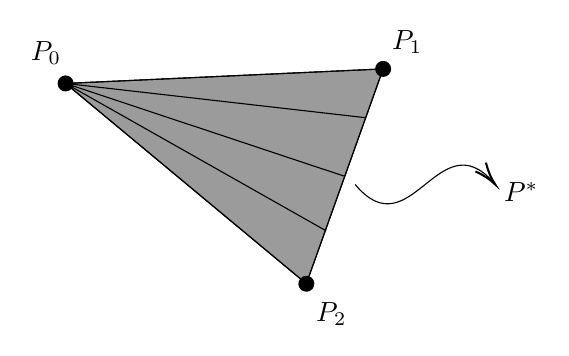
\begin{tikzpicture}[x=0.75pt,y=0.75pt,yscale=-1,xscale=1]
                %uncomment if require: \path (0,433); %set diagram left start at 0, and has height of 433

                %Shape: Polygon [id:ds6314772368856416] 
                \draw  [fill={rgb, 255:red, 155; green, 155; blue, 155 }  ,fill opacity=1 ] (299,122) -- (299,122) -- (262,225.5) -- (146,129) -- (146,129) -- cycle ;
                %Straight Lines [id:da3333010738727631] 
                \draw    (146,129) -- (262,225.5) ;
                \draw [shift={(262,225.5)}, rotate = 39.76] [color={rgb, 255:red, 0; green, 0; blue, 0 }  ][fill={rgb, 255:red, 0; green, 0; blue, 0 }  ][line width=0.75]      (0, 0) circle [x radius= 3.35, y radius= 3.35]   ;
                %Straight Lines [id:da8171687387763229] 
                \draw    (146,129) -- (299,122) ;
                \draw [shift={(299,122)}, rotate = 357.38] [color={rgb, 255:red, 0; green, 0; blue, 0 }  ][fill={rgb, 255:red, 0; green, 0; blue, 0 }  ][line width=0.75]      (0, 0) circle [x radius= 3.35, y radius= 3.35]   ;
                \draw [shift={(146,129)}, rotate = 357.38] [color={rgb, 255:red, 0; green, 0; blue, 0 }  ][fill={rgb, 255:red, 0; green, 0; blue, 0 }  ][line width=0.75]      (0, 0) circle [x radius= 3.35, y radius= 3.35]   ;
                %Straight Lines [id:da2622457736206354] 
                \draw    (299,122) -- (262,225.5) ;
                %Straight Lines [id:da8525045384135113] 
                \draw    (146,129) -- (290.5,145.5) ;
                %Straight Lines [id:da00542922010302771] 
                \draw    (146,129) -- (280.5,173.75) ;
                %Straight Lines [id:da6358953940151866] 
                \draw    (146,129) -- (271.5,200) ;
                %Shape: Boxed Bezier Curve [id:dp47251275539570226] 
                \draw    (285.5,177.67) .. controls (312.1,209.51) and (325.59,147.27) .. (351.79,176.28) ;
                \draw [shift={(353,177.67)}, rotate = 230.13] [color={rgb, 255:red, 0; green, 0; blue, 0 }  ][line width=0.75]    (10.93,-3.29) .. controls (6.95,-1.4) and (3.31,-0.3) .. (0,0) .. controls (3.31,0.3) and (6.95,1.4) .. (10.93,3.29)   ;

                % Text Node
                \draw (128,107.4) node [anchor=north west][inner sep=0.75pt]    {$P_{0}$};
                % Text Node
                \draw (302,102.4) node [anchor=north west][inner sep=0.75pt]    {$P_{1}$};
                % Text Node
                \draw (265.5,233.4) node [anchor=north west][inner sep=0.75pt]    {$P_{2}$};
                % Text Node
                \draw (356,175.4) node [anchor=north west][inner sep=0.75pt]    {$P^{*}$};


            \end{tikzpicture}

        \end{center}
    \item[k=3)] $\{P_0,P_1,P_2,P_3\}$ Un 3-simplesso è una piramide a base triangolare (tetraedro)
        \begin{center}


            \tikzset{every picture/.style={line width=0.75pt}} %set default line width to 0.75pt        

            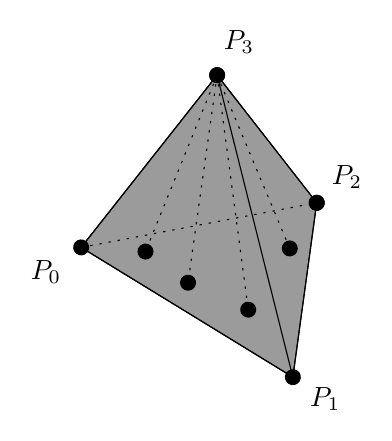
\begin{tikzpicture}[x=0.75pt,y=0.75pt,yscale=-1,xscale=1]
                %uncomment if require: \path (0,433); %set diagram left start at 0, and has height of 433

                %Shape: Polygon [id:ds22371152915300674] 
                \draw  [fill={rgb, 255:red, 155; green, 155; blue, 155 }  ,fill opacity=1 ] (173.5,36) -- (221.5,97.5) -- (210,181.5) -- (210,181.5) -- (108,119) -- cycle ;
                %Straight Lines [id:da4044842211191053] 
                \draw    (108,119) -- (210,181.5) ;
                %Straight Lines [id:da5467755816382549] 
                \draw  [dash pattern={on 0.84pt off 2.51pt}]  (108,119) -- (221.5,97.5) ;
                %Straight Lines [id:da9482113062868258] 
                \draw    (221.5,97.5) -- (210,181.5) ;
                \draw [shift={(210,181.5)}, rotate = 97.8] [color={rgb, 255:red, 0; green, 0; blue, 0 }  ][fill={rgb, 255:red, 0; green, 0; blue, 0 }  ][line width=0.75]      (0, 0) circle [x radius= 3.35, y radius= 3.35]   ;
                \draw [shift={(221.5,97.5)}, rotate = 97.8] [color={rgb, 255:red, 0; green, 0; blue, 0 }  ][fill={rgb, 255:red, 0; green, 0; blue, 0 }  ][line width=0.75]      (0, 0) circle [x radius= 3.35, y radius= 3.35]   ;
                %Straight Lines [id:da15637839317427682] 
                \draw    (108,119) -- (173.5,36) ;
                \draw [shift={(173.5,36)}, rotate = 308.28] [color={rgb, 255:red, 0; green, 0; blue, 0 }  ][fill={rgb, 255:red, 0; green, 0; blue, 0 }  ][line width=0.75]      (0, 0) circle [x radius= 3.35, y radius= 3.35]   ;
                \draw [shift={(108,119)}, rotate = 308.28] [color={rgb, 255:red, 0; green, 0; blue, 0 }  ][fill={rgb, 255:red, 0; green, 0; blue, 0 }  ][line width=0.75]      (0, 0) circle [x radius= 3.35, y radius= 3.35]   ;
                %Straight Lines [id:da34700462406010435] 
                \draw    (173.5,36) -- (221.5,97.5) ;
                \draw [shift={(221.5,97.5)}, rotate = 52.03] [color={rgb, 255:red, 0; green, 0; blue, 0 }  ][fill={rgb, 255:red, 0; green, 0; blue, 0 }  ][line width=0.75]      (0, 0) circle [x radius= 3.35, y radius= 3.35]   ;
                %Straight Lines [id:da8559731638239367] 
                \draw    (173.5,36) -- (210,181.5) ;
                %Straight Lines [id:da5585863272662528] 
                \draw  [dash pattern={on 0.84pt off 2.51pt}]  (173.5,36) -- (139,121) ;
                \draw [shift={(139,121)}, rotate = 112.09] [color={rgb, 255:red, 0; green, 0; blue, 0 }  ][fill={rgb, 255:red, 0; green, 0; blue, 0 }  ][line width=0.75]      (0, 0) circle [x radius= 3.35, y radius= 3.35]   ;
                \draw [shift={(173.5,36)}, rotate = 112.09] [color={rgb, 255:red, 0; green, 0; blue, 0 }  ][fill={rgb, 255:red, 0; green, 0; blue, 0 }  ][line width=0.75]      (0, 0) circle [x radius= 3.35, y radius= 3.35]   ;
                %Straight Lines [id:da71759991002901] 
                \draw  [dash pattern={on 0.84pt off 2.51pt}]  (173.5,36) -- (159.5,136) ;
                \draw [shift={(159.5,136)}, rotate = 97.97] [color={rgb, 255:red, 0; green, 0; blue, 0 }  ][fill={rgb, 255:red, 0; green, 0; blue, 0 }  ][line width=0.75]      (0, 0) circle [x radius= 3.35, y radius= 3.35]   ;
                %Straight Lines [id:da8455874170089126] 
                \draw  [dash pattern={on 0.84pt off 2.51pt}]  (173.5,36) -- (188.5,149) ;
                \draw [shift={(188.5,149)}, rotate = 82.44] [color={rgb, 255:red, 0; green, 0; blue, 0 }  ][fill={rgb, 255:red, 0; green, 0; blue, 0 }  ][line width=0.75]      (0, 0) circle [x radius= 3.35, y radius= 3.35]   ;
                %Straight Lines [id:da65302718613039] 
                \draw  [dash pattern={on 0.84pt off 2.51pt}]  (173.5,36) -- (208.5,119.5) ;
                \draw [shift={(208.5,119.5)}, rotate = 67.26] [color={rgb, 255:red, 0; green, 0; blue, 0 }  ][fill={rgb, 255:red, 0; green, 0; blue, 0 }  ][line width=0.75]      (0, 0) circle [x radius= 3.35, y radius= 3.35]   ;

                % Text Node
                \draw (82.5,123.9) node [anchor=north west][inner sep=0.75pt]    {$P_{0}$};
                % Text Node
                \draw (217,185.4) node [anchor=north west][inner sep=0.75pt]    {$P_{1}$};
                % Text Node
                \draw (227.5,78.4) node [anchor=north west][inner sep=0.75pt]    {$P_{2}$};
                % Text Node
                \draw (175.5,13.4) node [anchor=north west][inner sep=0.75pt]    {$P_{3}$};


            \end{tikzpicture}

        \end{center}
\end{enumerate}
\section{Proprietà generali}
\begin{definition}[Trasformazione affine]
    Una trasformazione affine in $\R^n$ è una composizione di una traslazione e di una trasformazione lineare invertibile
\end{definition}
\subsection{Proprietà 1}
Le trasformazioni affini conservano le proprietà di indipendenza geometrica, ossia dato un insieme di punti \pointset \geoind{i}, e una trasformazione affine
\[
    T:\R^n\ra\R^n
\]
allora
\[
    \{T(P_0),T(P_1),\dots,T(P_k)\}
\]
è un insieme di punti \geoind{i}
\subsection{Proprietà 2}
Per ogni insieme di punti \pointset \geoind{i}, esiste una trasformazione affine $T:\R^n\ra\R^n$ tale che
\begin{itemize}
    \item $T(P_0)=(0,\dots,0)$
    \item $\forall i=1,\dots,k$ $T(P_i-P_0)=\underline{e_i}$ (elemento i-esimo della base canonica di $\R^n$)
\end{itemize}
\paragraph{Intepretazione geometrica}
\begin{enumerate}
    \item [k=0)] Basta una traslazione del punto
          \begin{center}


              \tikzset{every picture/.style={line width=0.75pt}} %set default line width to 0.75pt        

              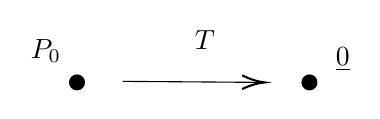
\begin{tikzpicture}[x=0.75pt,y=0.75pt,yscale=-1,xscale=1]
                  %uncomment if require: \path (0,433); %set diagram left start at 0, and has height of 433

                  %Straight Lines [id:da8368304048342596] 
                  \draw    (109.5,121) ;
                  \draw [shift={(109.5,121)}, rotate = 0] [color={rgb, 255:red, 0; green, 0; blue, 0 }  ][fill={rgb, 255:red, 0; green, 0; blue, 0 }  ][line width=0.75]      (0, 0) circle [x radius= 3.35, y radius= 3.35]   ;
                  %Straight Lines [id:da3167708141418948] 
                  \draw    (131.5,120.5) -- (198,120.99) ;
                  \draw [shift={(200,121)}, rotate = 180.42] [color={rgb, 255:red, 0; green, 0; blue, 0 }  ][line width=0.75]    (10.93,-3.29) .. controls (6.95,-1.4) and (3.31,-0.3) .. (0,0) .. controls (3.31,0.3) and (6.95,1.4) .. (10.93,3.29)   ;
                  %Shape: Boxed Line [id:dp7655619712630353] 
                  \draw    (221.5,121) ;
                  \draw [shift={(221.5,121)}, rotate = 0] [color={rgb, 255:red, 0; green, 0; blue, 0 }  ][fill={rgb, 255:red, 0; green, 0; blue, 0 }  ][line width=0.75]      (0, 0) circle [x radius= 3.35, y radius= 3.35]   ;

                  % Text Node
                  \draw (86,98.9) node [anchor=north west][inner sep=0.75pt]    {$P_{0}$};
                  % Text Node
                  \draw (233,102.9) node [anchor=north west][inner sep=0.75pt]    {$\underline{0}$};
                  % Text Node
                  \draw (165,94.9) node [anchor=north west][inner sep=0.75pt]    {$T$};


              \end{tikzpicture}

          \end{center}
          \pagebreak
    \item [k=1)] Serve una traslazione e una trasformazione lineare
          \begin{center}


              \tikzset{every picture/.style={line width=0.75pt}} %set default line width to 0.75pt        

              \begin{tikzpicture}[x=0.75pt,y=0.75pt,yscale=-1,xscale=1]
                  %uncomment if require: \path (0,433); %set diagram left start at 0, and has height of 433

                  %Straight Lines [id:da10241827211403942] 
                  \draw    (108,111) -- (179,162) ;
                  \draw [shift={(179,162)}, rotate = 35.69] [color={rgb, 255:red, 0; green, 0; blue, 0 }  ][fill={rgb, 255:red, 0; green, 0; blue, 0 }  ][line width=0.75]      (0, 0) circle [x radius= 3.35, y radius= 3.35]   ;
                  \draw [shift={(108,111)}, rotate = 35.69] [color={rgb, 255:red, 0; green, 0; blue, 0 }  ][fill={rgb, 255:red, 0; green, 0; blue, 0 }  ][line width=0.75]      (0, 0) circle [x radius= 3.35, y radius= 3.35]   ;
                  %Straight Lines [id:da8796603862462009] 
                  \draw    (210,130.5) -- (277,130.5) ;
                  \draw [shift={(279,130.5)}, rotate = 180] [color={rgb, 255:red, 0; green, 0; blue, 0 }  ][line width=0.75]    (10.93,-3.29) .. controls (6.95,-1.4) and (3.31,-0.3) .. (0,0) .. controls (3.31,0.3) and (6.95,1.4) .. (10.93,3.29)   ;
                  %Straight Lines [id:da9870700452278991] 
                  \draw    (299.5,130) -- (380,130.5) ;
                  \draw [shift={(380,130.5)}, rotate = 0.36] [color={rgb, 255:red, 0; green, 0; blue, 0 }  ][fill={rgb, 255:red, 0; green, 0; blue, 0 }  ][line width=0.75]      (0, 0) circle [x radius= 3.35, y radius= 3.35]   ;
                  \draw [shift={(299.5,130)}, rotate = 0.36] [color={rgb, 255:red, 0; green, 0; blue, 0 }  ][fill={rgb, 255:red, 0; green, 0; blue, 0 }  ][line width=0.75]      (0, 0) circle [x radius= 3.35, y radius= 3.35]   ;

                  % Text Node
                  \draw (89,87.4) node [anchor=north west][inner sep=0.75pt]    {$P_{0}$};
                  % Text Node
                  \draw (181,165.4) node [anchor=north west][inner sep=0.75pt]    {$P_{1}$};
                  % Text Node
                  \draw (240,139.4) node [anchor=north west][inner sep=0.75pt]    {$T$};
                  % Text Node
                  \draw (213.5,65.9) node [anchor=north west][inner sep=0.75pt]    {$P_{0} \longmapsto \underline{0}$};
                  % Text Node
                  \draw (178.5,91.4) node [anchor=north west][inner sep=0.75pt]    {$P_{1} \longmapsto ( 1,0,\dotsc ,0)$};


              \end{tikzpicture}

          \end{center}
    \item [k=2)] Serve una traslazione e una trasformazione lineare
          \begin{center}


              \tikzset{every picture/.style={line width=0.75pt}} %set default line width to 0.75pt        

              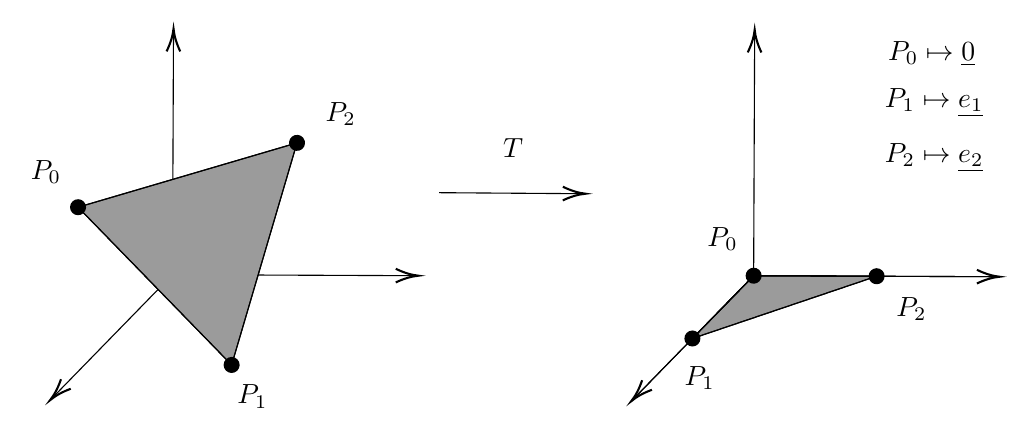
\begin{tikzpicture}[x=0.75pt,y=0.75pt,yscale=-1,xscale=1]
                  %uncomment if require: \path (0,433); %set diagram left start at 0, and has height of 433

                  %Shape: Polygon [id:ds48514589474210035] 
                  \draw  [fill={rgb, 255:red, 155; green, 155; blue, 155 }  ,fill opacity=1 ] (380.5,140) -- (439.75,140.25) -- (439.75,140.25) -- (351,170.25) -- (351,170.25) -- cycle ;
                  %Straight Lines [id:da071703597162452] 
                  \draw    (100.5,139.5) -- (42.9,198.57) ;
                  \draw [shift={(41.5,200)}, rotate = 314.28] [color={rgb, 255:red, 0; green, 0; blue, 0 }  ][line width=0.75]    (10.93,-3.29) .. controls (6.95,-1.4) and (3.31,-0.3) .. (0,0) .. controls (3.31,0.3) and (6.95,1.4) .. (10.93,3.29)   ;
                  %Shape: Boxed Line [id:dp531969180402829] 
                  \draw    (100.5,139.5) -- (217,139.99) ;
                  \draw [shift={(219,140)}, rotate = 180.24] [color={rgb, 255:red, 0; green, 0; blue, 0 }  ][line width=0.75]    (10.93,-3.29) .. controls (6.95,-1.4) and (3.31,-0.3) .. (0,0) .. controls (3.31,0.3) and (6.95,1.4) .. (10.93,3.29)   ;
                  %Straight Lines [id:da3249060433636406] 
                  \draw    (100.5,139.5) -- (100.99,23) ;
                  \draw [shift={(101,21)}, rotate = 90.24] [color={rgb, 255:red, 0; green, 0; blue, 0 }  ][line width=0.75]    (10.93,-3.29) .. controls (6.95,-1.4) and (3.31,-0.3) .. (0,0) .. controls (3.31,0.3) and (6.95,1.4) .. (10.93,3.29)   ;
                  %Shape: Polygon [id:ds054590197524766904] 
                  \draw  [fill={rgb, 255:red, 155; green, 155; blue, 155 }  ,fill opacity=1 ] (160.5,76) -- (160.5,76) -- (129,183) -- (129,183) -- (55,107) -- cycle ;
                  %Straight Lines [id:da8887250739730723] 
                  \draw    (55,107) -- (129,183) ;
                  \draw [shift={(129,183)}, rotate = 45.76] [color={rgb, 255:red, 0; green, 0; blue, 0 }  ][fill={rgb, 255:red, 0; green, 0; blue, 0 }  ][line width=0.75]      (0, 0) circle [x radius= 3.35, y radius= 3.35]   ;
                  \draw [shift={(55,107)}, rotate = 45.76] [color={rgb, 255:red, 0; green, 0; blue, 0 }  ][fill={rgb, 255:red, 0; green, 0; blue, 0 }  ][line width=0.75]      (0, 0) circle [x radius= 3.35, y radius= 3.35]   ;
                  %Straight Lines [id:da39797759845056113] 
                  \draw    (55,107) -- (160.5,76) ;
                  \draw [shift={(160.5,76)}, rotate = 343.63] [color={rgb, 255:red, 0; green, 0; blue, 0 }  ][fill={rgb, 255:red, 0; green, 0; blue, 0 }  ][line width=0.75]      (0, 0) circle [x radius= 3.35, y radius= 3.35]   ;
                  %Straight Lines [id:da4899451686599503] 
                  \draw    (160.5,76) -- (129,183) ;
                  %Straight Lines [id:da17448907454623375] 
                  \draw    (229,100) -- (297.5,100.49) ;
                  \draw [shift={(299.5,100.5)}, rotate = 180.41] [color={rgb, 255:red, 0; green, 0; blue, 0 }  ][line width=0.75]    (10.93,-3.29) .. controls (6.95,-1.4) and (3.31,-0.3) .. (0,0) .. controls (3.31,0.3) and (6.95,1.4) .. (10.93,3.29)   ;
                  %Straight Lines [id:da6453818746676654] 
                  \draw    (380.5,140) -- (322.9,199.07) ;
                  \draw [shift={(321.5,200.5)}, rotate = 314.28] [color={rgb, 255:red, 0; green, 0; blue, 0 }  ][line width=0.75]    (10.93,-3.29) .. controls (6.95,-1.4) and (3.31,-0.3) .. (0,0) .. controls (3.31,0.3) and (6.95,1.4) .. (10.93,3.29)   ;
                  %Shape: Boxed Line [id:dp7411775030014289] 
                  \draw    (380.5,140) -- (497,140.49) ;
                  \draw [shift={(499,140.5)}, rotate = 180.24] [color={rgb, 255:red, 0; green, 0; blue, 0 }  ][line width=0.75]    (10.93,-3.29) .. controls (6.95,-1.4) and (3.31,-0.3) .. (0,0) .. controls (3.31,0.3) and (6.95,1.4) .. (10.93,3.29)   ;
                  %Straight Lines [id:da7162075861471999] 
                  \draw    (380.5,140) -- (380.99,23.5) ;
                  \draw [shift={(381,21.5)}, rotate = 90.24] [color={rgb, 255:red, 0; green, 0; blue, 0 }  ][line width=0.75]    (10.93,-3.29) .. controls (6.95,-1.4) and (3.31,-0.3) .. (0,0) .. controls (3.31,0.3) and (6.95,1.4) .. (10.93,3.29)   ;
                  %Straight Lines [id:da9706295608445772] 
                  \draw    (380.5,140) -- (351,170.25) ;
                  \draw [shift={(351,170.25)}, rotate = 134.28] [color={rgb, 255:red, 0; green, 0; blue, 0 }  ][fill={rgb, 255:red, 0; green, 0; blue, 0 }  ][line width=0.75]      (0, 0) circle [x radius= 3.35, y radius= 3.35]   ;
                  \draw [shift={(380.5,140)}, rotate = 134.28] [color={rgb, 255:red, 0; green, 0; blue, 0 }  ][fill={rgb, 255:red, 0; green, 0; blue, 0 }  ][line width=0.75]      (0, 0) circle [x radius= 3.35, y radius= 3.35]   ;
                  %Straight Lines [id:da2464917220323657] 
                  \draw    (380.5,140) -- (439.75,140.25) ;
                  \draw [shift={(439.75,140.25)}, rotate = 0.24] [color={rgb, 255:red, 0; green, 0; blue, 0 }  ][fill={rgb, 255:red, 0; green, 0; blue, 0 }  ][line width=0.75]      (0, 0) circle [x radius= 3.35, y radius= 3.35]   ;
                  %Straight Lines [id:da1405812374368578] 
                  \draw    (380.5,140) -- (499,140.5) ;
                  %Straight Lines [id:da2207022877903011] 
                  \draw    (380.5,140) -- (321.5,200.5) ;
                  %Straight Lines [id:da3159859846403774] 
                  \draw    (439.75,140.25) -- (351,170.25) ;

                  % Text Node
                  \draw (31,83.4) node [anchor=north west][inner sep=0.75pt]    {$P_{0}$};
                  % Text Node
                  \draw (130.5,191.4) node [anchor=north west][inner sep=0.75pt]    {$P_{1}$};
                  % Text Node
                  \draw (173,55.4) node [anchor=north west][inner sep=0.75pt]    {$P_{2}$};
                  % Text Node
                  \draw (258.5,72.9) node [anchor=north west][inner sep=0.75pt]    {$T$};
                  % Text Node
                  \draw (357,115.4) node [anchor=north west][inner sep=0.75pt]    {$P_{0}$};
                  % Text Node
                  \draw (346,182.4) node [anchor=north west][inner sep=0.75pt]    {$P_{1}$};
                  % Text Node
                  \draw (448,149.4) node [anchor=north west][inner sep=0.75pt]    {$P_{2}$};
                  % Text Node
                  \draw (444,25.9) node [anchor=north west][inner sep=0.75pt]    {$P_{0} \mapsto \underline{0}$};
                  % Text Node
                  \draw (442.5,48.4) node [anchor=north west][inner sep=0.75pt]    {$P_{1} \mapsto \underline{e_{1}}$};
                  % Text Node
                  \draw (442.5,74.9) node [anchor=north west][inner sep=0.75pt]    {$P_{2} \mapsto \underline{e_{2}}$};


              \end{tikzpicture}

          \end{center}
\end{enumerate}
\begin{definition}[K-simplesso standard]
    In $\R^n$, il k-simplesso standard è il k-simplesso generato dai punti
    \[
        \begin{array}{ll}
            P_0=(0,\dots,0)   \\
            P_1=(1,0,\dots,0) \\
            \vdots            \\
            P_k=(0,\dots,0,\underset{\text{(pos. k)}}{1},0,\dots,0)
        \end{array}
    \]
\end{definition}
\paragraph{Proprietà 3}
Due k-simplessi $\tau,\sigma$ qualsiasi sono tra loro omeomorfi, infatti, prendiamo la trasformazione affine
\[
    T_\sigma:\R^n\ra\R^n
\]
tale che i punti \pointset che generano $\sigma$ vengono mandati nel k-simplesso standard $\omega$.\\
Le restrizioni
\[
    \left.T_\sigma\right|_{\sigma}\sigma\ra\omega
\]
\[
    \left.T_\tau\right|_{\tau}\tau\ra\omega
\]
le quali sono biunivoche.\\
Una trasformazione affine è continua per definizione, quindi le due restrizioni sono omeomorfismi. Inoltre
\[
    \begin{tikzcd}
        \sigma && \omega && \tau
        \arrow["{T_\sigma}", from=1-1, to=1-3]
        \arrow["{T_\tau^{-1}}", from=1-3, to=1-5]
        \arrow["{T_\sigma\circ T_\tau^{-1}}"', curve={height=30pt}, from=1-1, to=1-5]
    \end{tikzcd}
\]
ossia $\sigma$ e $\tau$ sono omeomorfi
\paragraph{Proprietà 4}
Le funzioni
\[
    t_i:\sigma\ra\R
\]
che corrispondono alle coordinate baricentriche del simplesso $\sigma$, sono funzioni continue (punti nel simplesso vicini tra loro hanno coordinate vicine tra loro)
\paragraph{Proprietà 5}
Il k-simplesso $\sigma$ è l'unione di tutti i segmenti che uniscono un vertice di $\sigma$ e un punto del k-1 simplesso generato dagli altri punti
\paragraph{Proprietà 6}
Per ogni k-simplesso, esiste un unico insieme di punti \geoind{i} che lo generano
\paragraph{Proprietà 7}
Un simplesso è un insieme connesso di $\R^n$
\begin{itemize}
    \item $\sigma$ è il più piccolo insieme connesso di $\R^n$ contenente i punti \pointset che generano $\sigma$
    \item $\sigma$ è l'insieme di tutti gli insiemi connessi di  $\R^n$ contenenti \pointset
    \item $\sigma$ è l'inviluppo convesso (convex hull) dei punti \pointset
\end{itemize}
\pagebreak
\section{Confronto combinatorio-topologico}
Consideriamo un k-simplesso $\sigma$ fissato generato da \pointset punti \geoind{i}
\begin{itemize}
    \item I punti \pointset si dicono vertici di $\sigma$
    \item $k$ si dice dimensione di $\sigma$
    \item Ogni simplesso generato da un sottoinsieme proprio di $h+1$ punti di \pointset si dice faccia del k-simplesso
          \subitem Le facce di dimensione 2 sono gli spigoli
          \subitem Le facce di dimensione 1 sono i vertici
          \begin{center}


              \tikzset{every picture/.style={line width=0.75pt}} %set default line width to 0.75pt        

              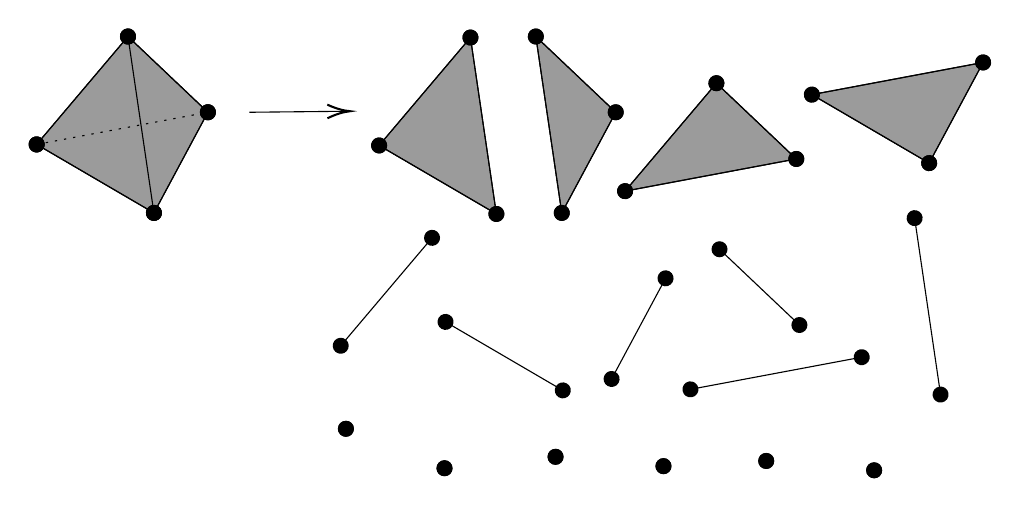
\begin{tikzpicture}[x=0.75pt,y=0.75pt,yscale=-1,xscale=1]
                  %uncomment if require: \path (0,433); %set diagram left start at 0, and has height of 433

                  %Shape: Polygon [id:ds2847770986922433] 
                  \draw  [fill={rgb, 255:red, 155; green, 155; blue, 155 }  ,fill opacity=1 ] (504,66.5) -- (478,115) -- (421.5,82) -- cycle ;
                  %Shape: Polygon [id:ds5561306825956198] 
                  \draw  [fill={rgb, 255:red, 155; green, 155; blue, 155 }  ,fill opacity=1 ] (375.5,76.5) -- (414,113) -- (331.5,128.5) -- cycle ;
                  %Shape: Polygon [id:ds4676262346176385] 
                  \draw  [fill={rgb, 255:red, 155; green, 155; blue, 155 }  ,fill opacity=1 ] (288.5,54) -- (327,90.5) -- (301,139) -- cycle ;
                  %Shape: Polygon [id:ds915223376332063] 
                  \draw  [fill={rgb, 255:red, 155; green, 155; blue, 155 }  ,fill opacity=1 ] (257,54.5) -- (269.5,139.5) -- (213,106.5) -- cycle ;
                  %Shape: Polygon [id:ds09840614435823869] 
                  \draw  [fill={rgb, 255:red, 155; green, 155; blue, 155 }  ,fill opacity=1 ] (92,54) -- (130.5,90.5) -- (104.5,139) -- (48,106) -- (48,106) -- cycle ;
                  %Straight Lines [id:da9037248559096869] 
                  \draw    (48,106) -- (104.5,139) ;
                  \draw [shift={(104.5,139)}, rotate = 30.29] [color={rgb, 255:red, 0; green, 0; blue, 0 }  ][fill={rgb, 255:red, 0; green, 0; blue, 0 }  ][line width=0.75]      (0, 0) circle [x radius= 3.35, y radius= 3.35]   ;
                  \draw [shift={(48,106)}, rotate = 30.29] [color={rgb, 255:red, 0; green, 0; blue, 0 }  ][fill={rgb, 255:red, 0; green, 0; blue, 0 }  ][line width=0.75]      (0, 0) circle [x radius= 3.35, y radius= 3.35]   ;
                  %Straight Lines [id:da32731019604578826] 
                  \draw    (104.5,139) -- (130.5,90.5) ;
                  \draw [shift={(130.5,90.5)}, rotate = 298.19] [color={rgb, 255:red, 0; green, 0; blue, 0 }  ][fill={rgb, 255:red, 0; green, 0; blue, 0 }  ][line width=0.75]      (0, 0) circle [x radius= 3.35, y radius= 3.35]   ;
                  \draw [shift={(104.5,139)}, rotate = 298.19] [color={rgb, 255:red, 0; green, 0; blue, 0 }  ][fill={rgb, 255:red, 0; green, 0; blue, 0 }  ][line width=0.75]      (0, 0) circle [x radius= 3.35, y radius= 3.35]   ;
                  %Straight Lines [id:da6976113293491542] 
                  \draw  [dash pattern={on 0.84pt off 2.51pt}]  (48,106) -- (130.5,90.5) ;
                  \draw [shift={(130.5,90.5)}, rotate = 349.36] [color={rgb, 255:red, 0; green, 0; blue, 0 }  ][fill={rgb, 255:red, 0; green, 0; blue, 0 }  ][line width=0.75]      (0, 0) circle [x radius= 3.35, y radius= 3.35]   ;
                  \draw [shift={(48,106)}, rotate = 349.36] [color={rgb, 255:red, 0; green, 0; blue, 0 }  ][fill={rgb, 255:red, 0; green, 0; blue, 0 }  ][line width=0.75]      (0, 0) circle [x radius= 3.35, y radius= 3.35]   ;
                  %Straight Lines [id:da3727911364383669] 
                  \draw    (48,106) -- (92,54) ;
                  \draw [shift={(92,54)}, rotate = 310.24] [color={rgb, 255:red, 0; green, 0; blue, 0 }  ][fill={rgb, 255:red, 0; green, 0; blue, 0 }  ][line width=0.75]      (0, 0) circle [x radius= 3.35, y radius= 3.35]   ;
                  \draw [shift={(48,106)}, rotate = 310.24] [color={rgb, 255:red, 0; green, 0; blue, 0 }  ][fill={rgb, 255:red, 0; green, 0; blue, 0 }  ][line width=0.75]      (0, 0) circle [x radius= 3.35, y radius= 3.35]   ;
                  %Straight Lines [id:da5366397319098948] 
                  \draw    (92,54) -- (104.5,139) ;
                  \draw [shift={(104.5,139)}, rotate = 81.63] [color={rgb, 255:red, 0; green, 0; blue, 0 }  ][fill={rgb, 255:red, 0; green, 0; blue, 0 }  ][line width=0.75]      (0, 0) circle [x radius= 3.35, y radius= 3.35]   ;
                  \draw [shift={(92,54)}, rotate = 81.63] [color={rgb, 255:red, 0; green, 0; blue, 0 }  ][fill={rgb, 255:red, 0; green, 0; blue, 0 }  ][line width=0.75]      (0, 0) circle [x radius= 3.35, y radius= 3.35]   ;
                  %Straight Lines [id:da15365619895868665] 
                  \draw    (92,54) -- (130.5,90.5) ;
                  \draw [shift={(130.5,90.5)}, rotate = 43.47] [color={rgb, 255:red, 0; green, 0; blue, 0 }  ][fill={rgb, 255:red, 0; green, 0; blue, 0 }  ][line width=0.75]      (0, 0) circle [x radius= 3.35, y radius= 3.35]   ;
                  \draw [shift={(92,54)}, rotate = 43.47] [color={rgb, 255:red, 0; green, 0; blue, 0 }  ][fill={rgb, 255:red, 0; green, 0; blue, 0 }  ][line width=0.75]      (0, 0) circle [x radius= 3.35, y radius= 3.35]   ;
                  %Straight Lines [id:da6208400405936805] 
                  \draw    (150.5,90.5) -- (197,90.02) ;
                  \draw [shift={(199,90)}, rotate = 179.41] [color={rgb, 255:red, 0; green, 0; blue, 0 }  ][line width=0.75]    (10.93,-3.29) .. controls (6.95,-1.4) and (3.31,-0.3) .. (0,0) .. controls (3.31,0.3) and (6.95,1.4) .. (10.93,3.29)   ;
                  %Straight Lines [id:da5331279996760019] 
                  \draw    (213,106.5) -- (269.5,139.5) ;
                  \draw [shift={(269.5,139.5)}, rotate = 30.29] [color={rgb, 255:red, 0; green, 0; blue, 0 }  ][fill={rgb, 255:red, 0; green, 0; blue, 0 }  ][line width=0.75]      (0, 0) circle [x radius= 3.35, y radius= 3.35]   ;
                  \draw [shift={(213,106.5)}, rotate = 30.29] [color={rgb, 255:red, 0; green, 0; blue, 0 }  ][fill={rgb, 255:red, 0; green, 0; blue, 0 }  ][line width=0.75]      (0, 0) circle [x radius= 3.35, y radius= 3.35]   ;
                  %Straight Lines [id:da5525675436410533] 
                  \draw    (213,106.5) -- (257,54.5) ;
                  \draw [shift={(257,54.5)}, rotate = 310.24] [color={rgb, 255:red, 0; green, 0; blue, 0 }  ][fill={rgb, 255:red, 0; green, 0; blue, 0 }  ][line width=0.75]      (0, 0) circle [x radius= 3.35, y radius= 3.35]   ;
                  \draw [shift={(213,106.5)}, rotate = 310.24] [color={rgb, 255:red, 0; green, 0; blue, 0 }  ][fill={rgb, 255:red, 0; green, 0; blue, 0 }  ][line width=0.75]      (0, 0) circle [x radius= 3.35, y radius= 3.35]   ;
                  %Straight Lines [id:da8246542020106744] 
                  \draw    (257,54.5) -- (269.5,139.5) ;
                  \draw [shift={(269.5,139.5)}, rotate = 81.63] [color={rgb, 255:red, 0; green, 0; blue, 0 }  ][fill={rgb, 255:red, 0; green, 0; blue, 0 }  ][line width=0.75]      (0, 0) circle [x radius= 3.35, y radius= 3.35]   ;
                  \draw [shift={(257,54.5)}, rotate = 81.63] [color={rgb, 255:red, 0; green, 0; blue, 0 }  ][fill={rgb, 255:red, 0; green, 0; blue, 0 }  ][line width=0.75]      (0, 0) circle [x radius= 3.35, y radius= 3.35]   ;
                  %Straight Lines [id:da9693069568578099] 
                  \draw    (301,139) -- (327,90.5) ;
                  \draw [shift={(327,90.5)}, rotate = 298.19] [color={rgb, 255:red, 0; green, 0; blue, 0 }  ][fill={rgb, 255:red, 0; green, 0; blue, 0 }  ][line width=0.75]      (0, 0) circle [x radius= 3.35, y radius= 3.35]   ;
                  \draw [shift={(301,139)}, rotate = 298.19] [color={rgb, 255:red, 0; green, 0; blue, 0 }  ][fill={rgb, 255:red, 0; green, 0; blue, 0 }  ][line width=0.75]      (0, 0) circle [x radius= 3.35, y radius= 3.35]   ;
                  %Straight Lines [id:da40691482156557424] 
                  \draw    (288.5,54) -- (301,139) ;
                  \draw [shift={(301,139)}, rotate = 81.63] [color={rgb, 255:red, 0; green, 0; blue, 0 }  ][fill={rgb, 255:red, 0; green, 0; blue, 0 }  ][line width=0.75]      (0, 0) circle [x radius= 3.35, y radius= 3.35]   ;
                  \draw [shift={(288.5,54)}, rotate = 81.63] [color={rgb, 255:red, 0; green, 0; blue, 0 }  ][fill={rgb, 255:red, 0; green, 0; blue, 0 }  ][line width=0.75]      (0, 0) circle [x radius= 3.35, y radius= 3.35]   ;
                  %Straight Lines [id:da9573081010557667] 
                  \draw    (288.5,54) -- (327,90.5) ;
                  \draw [shift={(327,90.5)}, rotate = 43.47] [color={rgb, 255:red, 0; green, 0; blue, 0 }  ][fill={rgb, 255:red, 0; green, 0; blue, 0 }  ][line width=0.75]      (0, 0) circle [x radius= 3.35, y radius= 3.35]   ;
                  \draw [shift={(288.5,54)}, rotate = 43.47] [color={rgb, 255:red, 0; green, 0; blue, 0 }  ][fill={rgb, 255:red, 0; green, 0; blue, 0 }  ][line width=0.75]      (0, 0) circle [x radius= 3.35, y radius= 3.35]   ;
                  %Straight Lines [id:da4516174297179756] 
                  \draw    (331.5,128.5) -- (414,113) ;
                  \draw [shift={(414,113)}, rotate = 349.36] [color={rgb, 255:red, 0; green, 0; blue, 0 }  ][fill={rgb, 255:red, 0; green, 0; blue, 0 }  ][line width=0.75]      (0, 0) circle [x radius= 3.35, y radius= 3.35]   ;
                  \draw [shift={(331.5,128.5)}, rotate = 349.36] [color={rgb, 255:red, 0; green, 0; blue, 0 }  ][fill={rgb, 255:red, 0; green, 0; blue, 0 }  ][line width=0.75]      (0, 0) circle [x radius= 3.35, y radius= 3.35]   ;
                  %Straight Lines [id:da9709820168322516] 
                  \draw    (331.5,128.5) -- (375.5,76.5) ;
                  \draw [shift={(375.5,76.5)}, rotate = 310.24] [color={rgb, 255:red, 0; green, 0; blue, 0 }  ][fill={rgb, 255:red, 0; green, 0; blue, 0 }  ][line width=0.75]      (0, 0) circle [x radius= 3.35, y radius= 3.35]   ;
                  \draw [shift={(331.5,128.5)}, rotate = 310.24] [color={rgb, 255:red, 0; green, 0; blue, 0 }  ][fill={rgb, 255:red, 0; green, 0; blue, 0 }  ][line width=0.75]      (0, 0) circle [x radius= 3.35, y radius= 3.35]   ;
                  %Straight Lines [id:da14333685475600633] 
                  \draw    (375.5,76.5) -- (414,113) ;
                  \draw [shift={(414,113)}, rotate = 43.47] [color={rgb, 255:red, 0; green, 0; blue, 0 }  ][fill={rgb, 255:red, 0; green, 0; blue, 0 }  ][line width=0.75]      (0, 0) circle [x radius= 3.35, y radius= 3.35]   ;
                  \draw [shift={(375.5,76.5)}, rotate = 43.47] [color={rgb, 255:red, 0; green, 0; blue, 0 }  ][fill={rgb, 255:red, 0; green, 0; blue, 0 }  ][line width=0.75]      (0, 0) circle [x radius= 3.35, y radius= 3.35]   ;
                  %Straight Lines [id:da4699676622963427] 
                  \draw    (421.5,82) -- (478,115) ;
                  \draw [shift={(478,115)}, rotate = 30.29] [color={rgb, 255:red, 0; green, 0; blue, 0 }  ][fill={rgb, 255:red, 0; green, 0; blue, 0 }  ][line width=0.75]      (0, 0) circle [x radius= 3.35, y radius= 3.35]   ;
                  \draw [shift={(421.5,82)}, rotate = 30.29] [color={rgb, 255:red, 0; green, 0; blue, 0 }  ][fill={rgb, 255:red, 0; green, 0; blue, 0 }  ][line width=0.75]      (0, 0) circle [x radius= 3.35, y radius= 3.35]   ;
                  %Straight Lines [id:da6383342915300774] 
                  \draw    (478,115) -- (504,66.5) ;
                  \draw [shift={(504,66.5)}, rotate = 298.19] [color={rgb, 255:red, 0; green, 0; blue, 0 }  ][fill={rgb, 255:red, 0; green, 0; blue, 0 }  ][line width=0.75]      (0, 0) circle [x radius= 3.35, y radius= 3.35]   ;
                  \draw [shift={(478,115)}, rotate = 298.19] [color={rgb, 255:red, 0; green, 0; blue, 0 }  ][fill={rgb, 255:red, 0; green, 0; blue, 0 }  ][line width=0.75]      (0, 0) circle [x radius= 3.35, y radius= 3.35]   ;
                  %Straight Lines [id:da3564228415939825] 
                  \draw    (421.5,82) -- (504,66.5) ;
                  \draw [shift={(504,66.5)}, rotate = 349.36] [color={rgb, 255:red, 0; green, 0; blue, 0 }  ][fill={rgb, 255:red, 0; green, 0; blue, 0 }  ][line width=0.75]      (0, 0) circle [x radius= 3.35, y radius= 3.35]   ;
                  \draw [shift={(421.5,82)}, rotate = 349.36] [color={rgb, 255:red, 0; green, 0; blue, 0 }  ][fill={rgb, 255:red, 0; green, 0; blue, 0 }  ][line width=0.75]      (0, 0) circle [x radius= 3.35, y radius= 3.35]   ;
                  %Straight Lines [id:da4992851711291826] 
                  \draw    (194.5,203) -- (238.5,151) ;
                  \draw [shift={(238.5,151)}, rotate = 310.24] [color={rgb, 255:red, 0; green, 0; blue, 0 }  ][fill={rgb, 255:red, 0; green, 0; blue, 0 }  ][line width=0.75]      (0, 0) circle [x radius= 3.35, y radius= 3.35]   ;
                  \draw [shift={(194.5,203)}, rotate = 310.24] [color={rgb, 255:red, 0; green, 0; blue, 0 }  ][fill={rgb, 255:red, 0; green, 0; blue, 0 }  ][line width=0.75]      (0, 0) circle [x radius= 3.35, y radius= 3.35]   ;
                  %Straight Lines [id:da4355068840510128] 
                  \draw    (471,141.5) -- (483.5,226.5) ;
                  \draw [shift={(483.5,226.5)}, rotate = 81.63] [color={rgb, 255:red, 0; green, 0; blue, 0 }  ][fill={rgb, 255:red, 0; green, 0; blue, 0 }  ][line width=0.75]      (0, 0) circle [x radius= 3.35, y radius= 3.35]   ;
                  \draw [shift={(471,141.5)}, rotate = 81.63] [color={rgb, 255:red, 0; green, 0; blue, 0 }  ][fill={rgb, 255:red, 0; green, 0; blue, 0 }  ][line width=0.75]      (0, 0) circle [x radius= 3.35, y radius= 3.35]   ;
                  %Straight Lines [id:da9931174438357209] 
                  \draw    (245,191.5) -- (301.5,224.5) ;
                  \draw [shift={(301.5,224.5)}, rotate = 30.29] [color={rgb, 255:red, 0; green, 0; blue, 0 }  ][fill={rgb, 255:red, 0; green, 0; blue, 0 }  ][line width=0.75]      (0, 0) circle [x radius= 3.35, y radius= 3.35]   ;
                  \draw [shift={(245,191.5)}, rotate = 30.29] [color={rgb, 255:red, 0; green, 0; blue, 0 }  ][fill={rgb, 255:red, 0; green, 0; blue, 0 }  ][line width=0.75]      (0, 0) circle [x radius= 3.35, y radius= 3.35]   ;
                  %Straight Lines [id:da22924216035050549] 
                  \draw    (377,156.5) -- (415.5,193) ;
                  \draw [shift={(415.5,193)}, rotate = 43.47] [color={rgb, 255:red, 0; green, 0; blue, 0 }  ][fill={rgb, 255:red, 0; green, 0; blue, 0 }  ][line width=0.75]      (0, 0) circle [x radius= 3.35, y radius= 3.35]   ;
                  \draw [shift={(377,156.5)}, rotate = 43.47] [color={rgb, 255:red, 0; green, 0; blue, 0 }  ][fill={rgb, 255:red, 0; green, 0; blue, 0 }  ][line width=0.75]      (0, 0) circle [x radius= 3.35, y radius= 3.35]   ;
                  %Straight Lines [id:da8162549315538588] 
                  \draw    (325,219) -- (351,170.5) ;
                  \draw [shift={(351,170.5)}, rotate = 298.19] [color={rgb, 255:red, 0; green, 0; blue, 0 }  ][fill={rgb, 255:red, 0; green, 0; blue, 0 }  ][line width=0.75]      (0, 0) circle [x radius= 3.35, y radius= 3.35]   ;
                  \draw [shift={(325,219)}, rotate = 298.19] [color={rgb, 255:red, 0; green, 0; blue, 0 }  ][fill={rgb, 255:red, 0; green, 0; blue, 0 }  ][line width=0.75]      (0, 0) circle [x radius= 3.35, y radius= 3.35]   ;
                  %Straight Lines [id:da14422932207632755] 
                  \draw    (363,224) -- (445.5,208.5) ;
                  \draw [shift={(445.5,208.5)}, rotate = 349.36] [color={rgb, 255:red, 0; green, 0; blue, 0 }  ][fill={rgb, 255:red, 0; green, 0; blue, 0 }  ][line width=0.75]      (0, 0) circle [x radius= 3.35, y radius= 3.35]   ;
                  \draw [shift={(363,224)}, rotate = 349.36] [color={rgb, 255:red, 0; green, 0; blue, 0 }  ][fill={rgb, 255:red, 0; green, 0; blue, 0 }  ][line width=0.75]      (0, 0) circle [x radius= 3.35, y radius= 3.35]   ;
                  %Shape: Boxed Line [id:dp5072062328159506] 
                  \draw    (197,243) ;
                  \draw [shift={(197,243)}, rotate = 0] [color={rgb, 255:red, 0; green, 0; blue, 0 }  ][fill={rgb, 255:red, 0; green, 0; blue, 0 }  ][line width=0.75]      (0, 0) circle [x radius= 3.35, y radius= 3.35]   ;
                  \draw [shift={(197,243)}, rotate = 0] [color={rgb, 255:red, 0; green, 0; blue, 0 }  ][fill={rgb, 255:red, 0; green, 0; blue, 0 }  ][line width=0.75]      (0, 0) circle [x radius= 3.35, y radius= 3.35]   ;
                  %Shape: Boxed Line [id:dp8306761309744515] 
                  \draw    (244.5,262) ;
                  \draw [shift={(244.5,262)}, rotate = 0] [color={rgb, 255:red, 0; green, 0; blue, 0 }  ][fill={rgb, 255:red, 0; green, 0; blue, 0 }  ][line width=0.75]      (0, 0) circle [x radius= 3.35, y radius= 3.35]   ;
                  \draw [shift={(244.5,262)}, rotate = 0] [color={rgb, 255:red, 0; green, 0; blue, 0 }  ][fill={rgb, 255:red, 0; green, 0; blue, 0 }  ][line width=0.75]      (0, 0) circle [x radius= 3.35, y radius= 3.35]   ;
                  %Shape: Boxed Line [id:dp45432684816024316] 
                  \draw    (298,256.5) ;
                  \draw [shift={(298,256.5)}, rotate = 0] [color={rgb, 255:red, 0; green, 0; blue, 0 }  ][fill={rgb, 255:red, 0; green, 0; blue, 0 }  ][line width=0.75]      (0, 0) circle [x radius= 3.35, y radius= 3.35]   ;
                  \draw [shift={(298,256.5)}, rotate = 0] [color={rgb, 255:red, 0; green, 0; blue, 0 }  ][fill={rgb, 255:red, 0; green, 0; blue, 0 }  ][line width=0.75]      (0, 0) circle [x radius= 3.35, y radius= 3.35]   ;
                  %Shape: Boxed Line [id:dp8000448490312111] 
                  \draw    (350,261) ;
                  \draw [shift={(350,261)}, rotate = 0] [color={rgb, 255:red, 0; green, 0; blue, 0 }  ][fill={rgb, 255:red, 0; green, 0; blue, 0 }  ][line width=0.75]      (0, 0) circle [x radius= 3.35, y radius= 3.35]   ;
                  \draw [shift={(350,261)}, rotate = 0] [color={rgb, 255:red, 0; green, 0; blue, 0 }  ][fill={rgb, 255:red, 0; green, 0; blue, 0 }  ][line width=0.75]      (0, 0) circle [x radius= 3.35, y radius= 3.35]   ;
                  %Shape: Boxed Line [id:dp30431705621524974] 
                  \draw    (399.5,258.5) ;
                  \draw [shift={(399.5,258.5)}, rotate = 0] [color={rgb, 255:red, 0; green, 0; blue, 0 }  ][fill={rgb, 255:red, 0; green, 0; blue, 0 }  ][line width=0.75]      (0, 0) circle [x radius= 3.35, y radius= 3.35]   ;
                  \draw [shift={(399.5,258.5)}, rotate = 0] [color={rgb, 255:red, 0; green, 0; blue, 0 }  ][fill={rgb, 255:red, 0; green, 0; blue, 0 }  ][line width=0.75]      (0, 0) circle [x radius= 3.35, y radius= 3.35]   ;
                  %Shape: Boxed Line [id:dp29424857420031514] 
                  \draw    (451.5,263) ;
                  \draw [shift={(451.5,263)}, rotate = 0] [color={rgb, 255:red, 0; green, 0; blue, 0 }  ][fill={rgb, 255:red, 0; green, 0; blue, 0 }  ][line width=0.75]      (0, 0) circle [x radius= 3.35, y radius= 3.35]   ;
                  \draw [shift={(451.5,263)}, rotate = 0] [color={rgb, 255:red, 0; green, 0; blue, 0 }  ][fill={rgb, 255:red, 0; green, 0; blue, 0 }  ][line width=0.75]      (0, 0) circle [x radius= 3.35, y radius= 3.35]   ;




              \end{tikzpicture}

          \end{center}
    \item Le facce di dimensione $k-1$ si dicono facce massimali (o facet)
    \item Dato un simplesso $\sigma$, l'unione di tutte le facce di $\sigma$ si dice bordo di $\sigma$ ($Bd(\sigma)$)
          \begin{center}


              \tikzset{every picture/.style={line width=0.75pt}} %set default line width to 0.75pt        

              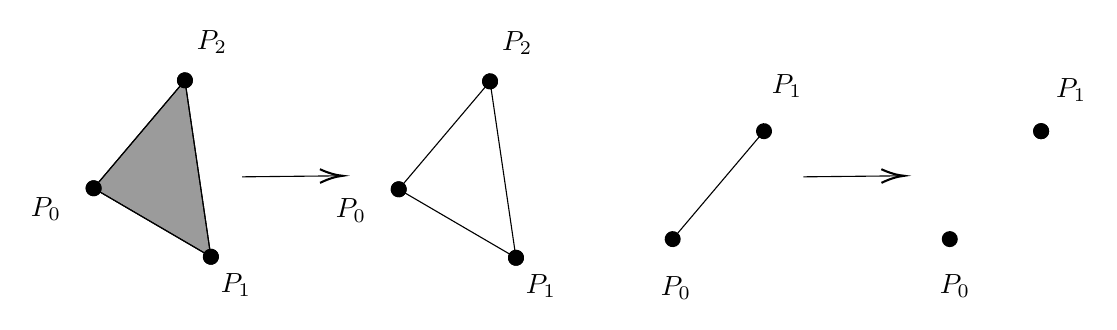
\begin{tikzpicture}[x=0.75pt,y=0.75pt,yscale=-1,xscale=1]
                  %uncomment if require: \path (0,433); %set diagram left start at 0, and has height of 433

                  %Shape: Polygon [id:ds915223376332063] 
                  \draw  [fill={rgb, 255:red, 155; green, 155; blue, 155 }  ,fill opacity=1 ] (123,44) -- (135.5,129) -- (79,96) -- cycle ;
                  %Straight Lines [id:da6208400405936805] 
                  \draw    (150.5,90.5) -- (197,90.02) ;
                  \draw [shift={(199,90)}, rotate = 179.41] [color={rgb, 255:red, 0; green, 0; blue, 0 }  ][line width=0.75]    (10.93,-3.29) .. controls (6.95,-1.4) and (3.31,-0.3) .. (0,0) .. controls (3.31,0.3) and (6.95,1.4) .. (10.93,3.29)   ;
                  %Straight Lines [id:da5331279996760019] 
                  \draw    (79,96) -- (135.5,129) ;
                  \draw [shift={(135.5,129)}, rotate = 30.29] [color={rgb, 255:red, 0; green, 0; blue, 0 }  ][fill={rgb, 255:red, 0; green, 0; blue, 0 }  ][line width=0.75]      (0, 0) circle [x radius= 3.35, y radius= 3.35]   ;
                  \draw [shift={(79,96)}, rotate = 30.29] [color={rgb, 255:red, 0; green, 0; blue, 0 }  ][fill={rgb, 255:red, 0; green, 0; blue, 0 }  ][line width=0.75]      (0, 0) circle [x radius= 3.35, y radius= 3.35]   ;
                  %Straight Lines [id:da5525675436410533] 
                  \draw    (79,96) -- (123,44) ;
                  \draw [shift={(123,44)}, rotate = 310.24] [color={rgb, 255:red, 0; green, 0; blue, 0 }  ][fill={rgb, 255:red, 0; green, 0; blue, 0 }  ][line width=0.75]      (0, 0) circle [x radius= 3.35, y radius= 3.35]   ;
                  \draw [shift={(79,96)}, rotate = 310.24] [color={rgb, 255:red, 0; green, 0; blue, 0 }  ][fill={rgb, 255:red, 0; green, 0; blue, 0 }  ][line width=0.75]      (0, 0) circle [x radius= 3.35, y radius= 3.35]   ;
                  %Straight Lines [id:da8246542020106744] 
                  \draw    (123,44) -- (135.5,129) ;
                  \draw [shift={(135.5,129)}, rotate = 81.63] [color={rgb, 255:red, 0; green, 0; blue, 0 }  ][fill={rgb, 255:red, 0; green, 0; blue, 0 }  ][line width=0.75]      (0, 0) circle [x radius= 3.35, y radius= 3.35]   ;
                  \draw [shift={(123,44)}, rotate = 81.63] [color={rgb, 255:red, 0; green, 0; blue, 0 }  ][fill={rgb, 255:red, 0; green, 0; blue, 0 }  ][line width=0.75]      (0, 0) circle [x radius= 3.35, y radius= 3.35]   ;
                  %Straight Lines [id:da4992851711291826] 
                  \draw    (358,120.5) -- (402,68.5) ;
                  \draw [shift={(402,68.5)}, rotate = 310.24] [color={rgb, 255:red, 0; green, 0; blue, 0 }  ][fill={rgb, 255:red, 0; green, 0; blue, 0 }  ][line width=0.75]      (0, 0) circle [x radius= 3.35, y radius= 3.35]   ;
                  \draw [shift={(358,120.5)}, rotate = 310.24] [color={rgb, 255:red, 0; green, 0; blue, 0 }  ][fill={rgb, 255:red, 0; green, 0; blue, 0 }  ][line width=0.75]      (0, 0) circle [x radius= 3.35, y radius= 3.35]   ;
                  %Straight Lines [id:da877655332560483] 
                  \draw    (421,90.5) -- (467.5,90.02) ;
                  \draw [shift={(469.5,90)}, rotate = 179.41] [color={rgb, 255:red, 0; green, 0; blue, 0 }  ][line width=0.75]    (10.93,-3.29) .. controls (6.95,-1.4) and (3.31,-0.3) .. (0,0) .. controls (3.31,0.3) and (6.95,1.4) .. (10.93,3.29)   ;
                  %Straight Lines [id:da5031383725475427] 
                  \draw    (226,96.5) -- (282.5,129.5) ;
                  \draw [shift={(282.5,129.5)}, rotate = 30.29] [color={rgb, 255:red, 0; green, 0; blue, 0 }  ][fill={rgb, 255:red, 0; green, 0; blue, 0 }  ][line width=0.75]      (0, 0) circle [x radius= 3.35, y radius= 3.35]   ;
                  \draw [shift={(226,96.5)}, rotate = 30.29] [color={rgb, 255:red, 0; green, 0; blue, 0 }  ][fill={rgb, 255:red, 0; green, 0; blue, 0 }  ][line width=0.75]      (0, 0) circle [x radius= 3.35, y radius= 3.35]   ;
                  %Straight Lines [id:da687799715442041] 
                  \draw    (226,96.5) -- (270,44.5) ;
                  \draw [shift={(270,44.5)}, rotate = 310.24] [color={rgb, 255:red, 0; green, 0; blue, 0 }  ][fill={rgb, 255:red, 0; green, 0; blue, 0 }  ][line width=0.75]      (0, 0) circle [x radius= 3.35, y radius= 3.35]   ;
                  \draw [shift={(226,96.5)}, rotate = 310.24] [color={rgb, 255:red, 0; green, 0; blue, 0 }  ][fill={rgb, 255:red, 0; green, 0; blue, 0 }  ][line width=0.75]      (0, 0) circle [x radius= 3.35, y radius= 3.35]   ;
                  %Straight Lines [id:da8266341552377607] 
                  \draw    (270,44.5) -- (282.5,129.5) ;
                  \draw [shift={(282.5,129.5)}, rotate = 81.63] [color={rgb, 255:red, 0; green, 0; blue, 0 }  ][fill={rgb, 255:red, 0; green, 0; blue, 0 }  ][line width=0.75]      (0, 0) circle [x radius= 3.35, y radius= 3.35]   ;
                  \draw [shift={(270,44.5)}, rotate = 81.63] [color={rgb, 255:red, 0; green, 0; blue, 0 }  ][fill={rgb, 255:red, 0; green, 0; blue, 0 }  ][line width=0.75]      (0, 0) circle [x radius= 3.35, y radius= 3.35]   ;
                  %Straight Lines [id:da47525009972494536] 
                  \draw    (535.5,68.5) ;
                  \draw [shift={(535.5,68.5)}, rotate = 0] [color={rgb, 255:red, 0; green, 0; blue, 0 }  ][fill={rgb, 255:red, 0; green, 0; blue, 0 }  ][line width=0.75]      (0, 0) circle [x radius= 3.35, y radius= 3.35]   ;
                  \draw [shift={(535.5,68.5)}, rotate = 0] [color={rgb, 255:red, 0; green, 0; blue, 0 }  ][fill={rgb, 255:red, 0; green, 0; blue, 0 }  ][line width=0.75]      (0, 0) circle [x radius= 3.35, y radius= 3.35]   ;
                  %Straight Lines [id:da06269720981097349] 
                  \draw    (491.5,120.5) ;
                  \draw [shift={(491.5,120.5)}, rotate = 0] [color={rgb, 255:red, 0; green, 0; blue, 0 }  ][fill={rgb, 255:red, 0; green, 0; blue, 0 }  ][line width=0.75]      (0, 0) circle [x radius= 3.35, y radius= 3.35]   ;

                  % Text Node
                  \draw (47.5,99.4) node [anchor=north west][inner sep=0.75pt]    {$P_{0}$};
                  % Text Node
                  \draw (139,135.9) node [anchor=north west][inner sep=0.75pt]    {$P_{1}$};
                  % Text Node
                  \draw (127.5,18.9) node [anchor=north west][inner sep=0.75pt]    {$P_{2}$};
                  % Text Node
                  \draw (194.5,99.9) node [anchor=north west][inner sep=0.75pt]    {$P_{0}$};
                  % Text Node
                  \draw (286,136.4) node [anchor=north west][inner sep=0.75pt]    {$P_{1}$};
                  % Text Node
                  \draw (274.5,19.4) node [anchor=north west][inner sep=0.75pt]    {$P_{2}$};
                  % Text Node
                  \draw (351,137.4) node [anchor=north west][inner sep=0.75pt]    {$P_{0}$};
                  % Text Node
                  \draw (404.5,39.9) node [anchor=north west][inner sep=0.75pt]    {$P_{1}$};
                  % Text Node
                  \draw (485.5,136.4) node [anchor=north west][inner sep=0.75pt]    {$P_{0}$};
                  % Text Node
                  \draw (541.5,41.9) node [anchor=north west][inner sep=0.75pt]    {$P_{1}$};


              \end{tikzpicture}

          \end{center}
          \pagebreak
    \item Dato un simplesso $\sigma$, chiamiamo parte interna o interno di $\sigma$ la differenza tra $\sigma$ e il suo bordo
          \[
              Int(\sigma):=\sigma\setminus Bd(\sigma)
          \]
          \begin{center}


              \tikzset{every picture/.style={line width=0.75pt}} %set default line width to 0.75pt        

              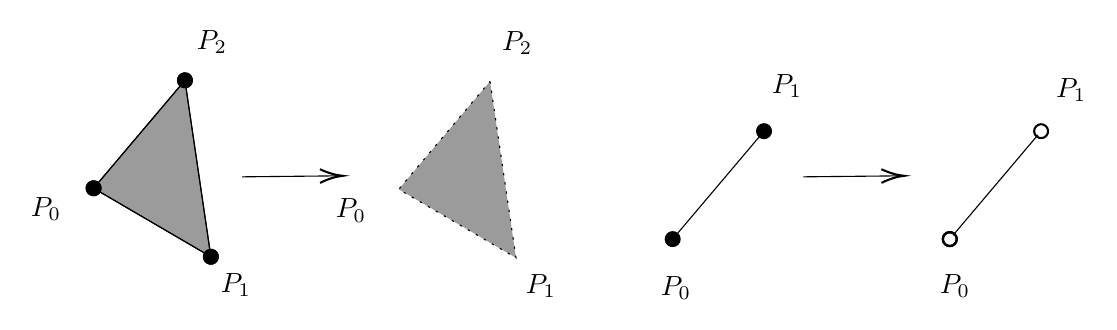
\begin{tikzpicture}[x=0.75pt,y=0.75pt,yscale=-1,xscale=1]
                  %uncomment if require: \path (0,433); %set diagram left start at 0, and has height of 433

                  %Shape: Polygon [id:ds8274177278959294] 
                  \draw  [fill={rgb, 255:red, 155; green, 155; blue, 155 }  ,fill opacity=1 ][dash pattern={on 0.84pt off 2.51pt}] (270,44.5) -- (282.5,129.5) -- (226,96.5) -- cycle ;
                  %Shape: Polygon [id:ds915223376332063] 
                  \draw  [fill={rgb, 255:red, 155; green, 155; blue, 155 }  ,fill opacity=1 ] (123,44) -- (135.5,129) -- (79,96) -- cycle ;
                  %Straight Lines [id:da6208400405936805] 
                  \draw    (150.5,90.5) -- (197,90.02) ;
                  \draw [shift={(199,90)}, rotate = 179.41] [color={rgb, 255:red, 0; green, 0; blue, 0 }  ][line width=0.75]    (10.93,-3.29) .. controls (6.95,-1.4) and (3.31,-0.3) .. (0,0) .. controls (3.31,0.3) and (6.95,1.4) .. (10.93,3.29)   ;
                  %Straight Lines [id:da5331279996760019] 
                  \draw    (79,96) -- (135.5,129) ;
                  \draw [shift={(135.5,129)}, rotate = 30.29] [color={rgb, 255:red, 0; green, 0; blue, 0 }  ][fill={rgb, 255:red, 0; green, 0; blue, 0 }  ][line width=0.75]      (0, 0) circle [x radius= 3.35, y radius= 3.35]   ;
                  \draw [shift={(79,96)}, rotate = 30.29] [color={rgb, 255:red, 0; green, 0; blue, 0 }  ][fill={rgb, 255:red, 0; green, 0; blue, 0 }  ][line width=0.75]      (0, 0) circle [x radius= 3.35, y radius= 3.35]   ;
                  %Straight Lines [id:da5525675436410533] 
                  \draw    (79,96) -- (123,44) ;
                  \draw [shift={(123,44)}, rotate = 310.24] [color={rgb, 255:red, 0; green, 0; blue, 0 }  ][fill={rgb, 255:red, 0; green, 0; blue, 0 }  ][line width=0.75]      (0, 0) circle [x radius= 3.35, y radius= 3.35]   ;
                  \draw [shift={(79,96)}, rotate = 310.24] [color={rgb, 255:red, 0; green, 0; blue, 0 }  ][fill={rgb, 255:red, 0; green, 0; blue, 0 }  ][line width=0.75]      (0, 0) circle [x radius= 3.35, y radius= 3.35]   ;
                  %Straight Lines [id:da8246542020106744] 
                  \draw    (123,44) -- (135.5,129) ;
                  \draw [shift={(135.5,129)}, rotate = 81.63] [color={rgb, 255:red, 0; green, 0; blue, 0 }  ][fill={rgb, 255:red, 0; green, 0; blue, 0 }  ][line width=0.75]      (0, 0) circle [x radius= 3.35, y radius= 3.35]   ;
                  \draw [shift={(123,44)}, rotate = 81.63] [color={rgb, 255:red, 0; green, 0; blue, 0 }  ][fill={rgb, 255:red, 0; green, 0; blue, 0 }  ][line width=0.75]      (0, 0) circle [x radius= 3.35, y radius= 3.35]   ;
                  %Straight Lines [id:da4992851711291826] 
                  \draw    (358,120.5) -- (402,68.5) ;
                  \draw [shift={(402,68.5)}, rotate = 310.24] [color={rgb, 255:red, 0; green, 0; blue, 0 }  ][fill={rgb, 255:red, 0; green, 0; blue, 0 }  ][line width=0.75]      (0, 0) circle [x radius= 3.35, y radius= 3.35]   ;
                  \draw [shift={(358,120.5)}, rotate = 310.24] [color={rgb, 255:red, 0; green, 0; blue, 0 }  ][fill={rgb, 255:red, 0; green, 0; blue, 0 }  ][line width=0.75]      (0, 0) circle [x radius= 3.35, y radius= 3.35]   ;
                  %Straight Lines [id:da877655332560483] 
                  \draw    (421,90.5) -- (467.5,90.02) ;
                  \draw [shift={(469.5,90)}, rotate = 179.41] [color={rgb, 255:red, 0; green, 0; blue, 0 }  ][line width=0.75]    (10.93,-3.29) .. controls (6.95,-1.4) and (3.31,-0.3) .. (0,0) .. controls (3.31,0.3) and (6.95,1.4) .. (10.93,3.29)   ;
                  %Straight Lines [id:da47525009972494536] 
                  \draw    (533.98,70.29) -- (493.02,118.71) ;
                  \draw [shift={(491.5,120.5)}, rotate = 130.24] [color={rgb, 255:red, 0; green, 0; blue, 0 }  ][line width=0.75]      (0, 0) circle [x radius= 3.35, y radius= 3.35]   ;
                  \draw [shift={(535.5,68.5)}, rotate = 130.24] [color={rgb, 255:red, 0; green, 0; blue, 0 }  ][line width=0.75]      (0, 0) circle [x radius= 3.35, y radius= 3.35]   ;
                  %Straight Lines [id:da06269720981097349] 
                  \draw    (491.5,120.5) ;
                  \draw [shift={(491.5,120.5)}, rotate = 0] [color={rgb, 255:red, 0; green, 0; blue, 0 }  ][line width=0.75]      (0, 0) circle [x radius= 3.35, y radius= 3.35]   ;
                  \draw [shift={(491.5,120.5)}, rotate = 0] [color={rgb, 255:red, 0; green, 0; blue, 0 }  ][line width=0.75]      (0, 0) circle [x radius= 3.35, y radius= 3.35]   ;

                  % Text Node
                  \draw (47.5,99.4) node [anchor=north west][inner sep=0.75pt]    {$P_{0}$};
                  % Text Node
                  \draw (139,135.9) node [anchor=north west][inner sep=0.75pt]    {$P_{1}$};
                  % Text Node
                  \draw (127.5,18.9) node [anchor=north west][inner sep=0.75pt]    {$P_{2}$};
                  % Text Node
                  \draw (194.5,99.9) node [anchor=north west][inner sep=0.75pt]    {$P_{0}$};
                  % Text Node
                  \draw (286,136.4) node [anchor=north west][inner sep=0.75pt]    {$P_{1}$};
                  % Text Node
                  \draw (274.5,19.4) node [anchor=north west][inner sep=0.75pt]    {$P_{2}$};
                  % Text Node
                  \draw (351,137.4) node [anchor=north west][inner sep=0.75pt]    {$P_{0}$};
                  % Text Node
                  \draw (404.5,39.9) node [anchor=north west][inner sep=0.75pt]    {$P_{1}$};
                  % Text Node
                  \draw (485.5,136.4) node [anchor=north west][inner sep=0.75pt]    {$P_{0}$};
                  % Text Node
                  \draw (541.5,41.9) node [anchor=north west][inner sep=0.75pt]    {$P_{1}$};


              \end{tikzpicture}

          \end{center}
\end{itemize}
Possiamo riscrivere le definizioni di bordo e interno come segue
\[
    \sigma:=\setst{x=\sum_{i=0}^k t_iP_i}{\sum_{i=0}^k t_i=1,\quad t_i\geq 0\quad\forall i=0,\dots,k}
\]
\[
    Int(\sigma):=\setst{x=\sum_{i=0}^k t_iP_i}{\sum_{i=0}^k t_i=1,\quad t_i> 0\quad\forall i=0,\dots,k}
\]
\[
    Bd(\sigma):=\setst{x=\sum_{i=0}^k t_iP_i}{\sum_{i=0}^k t_i=1,\quad \prod_{i=0}^k t_i=0}
\]
\paragraph{Osservazione}
Il numero di ceofficenti nulli ci informano della dimensione della faccia che stiamo considerano
\begin{itemize}
    \item 1 coefficiente nullo $\ra$ faccia massimale
    \item 2 coefficienti nulli $\ra$ faccia di dimensione $k-2$
\end{itemize}
\section{Proprietà topologiche k-simplessi}
Sia $\sigma\subseteq\R^n$ un k-simplesso
\begin{itemize}
    \item $\sigma$ è connesso, chiuso, limitato (ossia compatto)
    \item $Int(\sigma)\subseteq\R^n$ è l'unione di tutti i segmenti aperti (senza i due estremi) che collegano un vertice e i punti interni alla faccia massimale opposta.\\
          \begin{center}


              \tikzset{every picture/.style={line width=0.75pt}} %set default line width to 0.75pt        

              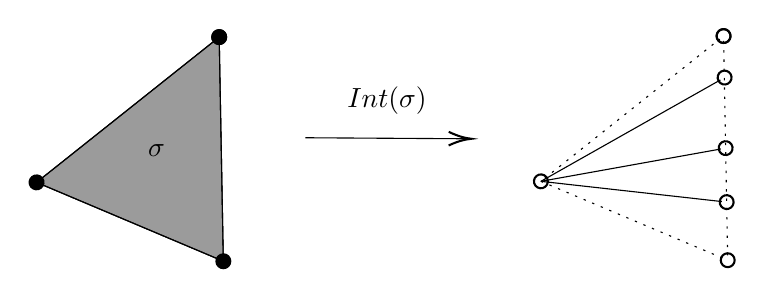
\begin{tikzpicture}[x=0.75pt,y=0.75pt,yscale=-1,xscale=1]
                  %uncomment if require: \path (0,433); %set diagram left start at 0, and has height of 433

                  %Shape: Polygon [id:ds9341310528457372] 
                  \draw  [fill={rgb, 255:red, 155; green, 155; blue, 155 }  ,fill opacity=1 ] (140,139.5) -- (50,101.5) -- (138,31.5) -- cycle ;
                  %Straight Lines [id:da9884943319383497] 
                  \draw    (50,101.5) -- (138,31.5) ;
                  \draw [shift={(138,31.5)}, rotate = 321.5] [color={rgb, 255:red, 0; green, 0; blue, 0 }  ][fill={rgb, 255:red, 0; green, 0; blue, 0 }  ][line width=0.75]      (0, 0) circle [x radius= 3.35, y radius= 3.35]   ;
                  \draw [shift={(50,101.5)}, rotate = 321.5] [color={rgb, 255:red, 0; green, 0; blue, 0 }  ][fill={rgb, 255:red, 0; green, 0; blue, 0 }  ][line width=0.75]      (0, 0) circle [x radius= 3.35, y radius= 3.35]   ;
                  %Straight Lines [id:da8473386968859349] 
                  \draw    (50,101.5) -- (140,139.5) ;
                  %Straight Lines [id:da368832108298889] 
                  \draw    (138,31.5) -- (140,139.5) ;
                  \draw [shift={(140,139.5)}, rotate = 88.94] [color={rgb, 255:red, 0; green, 0; blue, 0 }  ][fill={rgb, 255:red, 0; green, 0; blue, 0 }  ][line width=0.75]      (0, 0) circle [x radius= 3.35, y radius= 3.35]   ;
                  \draw [shift={(138,31.5)}, rotate = 88.94] [color={rgb, 255:red, 0; green, 0; blue, 0 }  ][fill={rgb, 255:red, 0; green, 0; blue, 0 }  ][line width=0.75]      (0, 0) circle [x radius= 3.35, y radius= 3.35]   ;
                  %Straight Lines [id:da9409885325805156] 
                  \draw  [dash pattern={on 0.84pt off 2.51pt}]  (294.84,99.54) -- (379.16,32.46) ;
                  \draw [shift={(381,31)}, rotate = 321.5] [color={rgb, 255:red, 0; green, 0; blue, 0 }  ][line width=0.75]      (0, 0) circle [x radius= 3.35, y radius= 3.35]   ;
                  \draw [shift={(293,101)}, rotate = 321.5] [color={rgb, 255:red, 0; green, 0; blue, 0 }  ][line width=0.75]      (0, 0) circle [x radius= 3.35, y radius= 3.35]   ;
                  %Straight Lines [id:da7518503078636023] 
                  \draw  [dash pattern={on 0.84pt off 2.51pt}]  (293,101) -- (383,139) ;
                  %Straight Lines [id:da3597474603551267] 
                  \draw  [dash pattern={on 0.84pt off 2.51pt}]  (381.04,33.35) -- (382.96,136.65) ;
                  \draw [shift={(383,139)}, rotate = 88.94] [color={rgb, 255:red, 0; green, 0; blue, 0 }  ][line width=0.75]      (0, 0) circle [x radius= 3.35, y radius= 3.35]   ;
                  \draw [shift={(381,31)}, rotate = 88.94] [color={rgb, 255:red, 0; green, 0; blue, 0 }  ][line width=0.75]      (0, 0) circle [x radius= 3.35, y radius= 3.35]   ;
                  %Straight Lines [id:da5190097278289834] 
                  \draw    (179.5,80) -- (257.5,80.49) ;
                  \draw [shift={(259.5,80.5)}, rotate = 180.36] [color={rgb, 255:red, 0; green, 0; blue, 0 }  ][line width=0.75]    (10.93,-3.29) .. controls (6.95,-1.4) and (3.31,-0.3) .. (0,0) .. controls (3.31,0.3) and (6.95,1.4) .. (10.93,3.29)   ;
                  %Straight Lines [id:da17420566916420155] 
                  \draw    (293,101) -- (379.69,85.42) ;
                  \draw [shift={(382,85)}, rotate = 349.81] [color={rgb, 255:red, 0; green, 0; blue, 0 }  ][line width=0.75]      (0, 0) circle [x radius= 3.35, y radius= 3.35]   ;
                  %Straight Lines [id:da9326780321362951] 
                  \draw    (293,101) -- (380.16,110.74) ;
                  \draw [shift={(382.5,111)}, rotate = 6.38] [color={rgb, 255:red, 0; green, 0; blue, 0 }  ][line width=0.75]      (0, 0) circle [x radius= 3.35, y radius= 3.35]   ;
                  %Straight Lines [id:da9538755048457965] 
                  \draw    (293,101) -- (379.45,52.16) ;
                  \draw [shift={(381.5,51)}, rotate = 330.53] [color={rgb, 255:red, 0; green, 0; blue, 0 }  ][line width=0.75]      (0, 0) circle [x radius= 3.35, y radius= 3.35]   ;

                  % Text Node
                  \draw (198.5,54.4) node [anchor=north west][inner sep=0.75pt]    {$Int( \sigma )$};
                  % Text Node
                  \draw (102.5,81.9) node [anchor=north west][inner sep=0.75pt]    {$\sigma $};


              \end{tikzpicture}

          \end{center}
          Non abbiamo perso la convessità, è $Int(\sigma)$ è aperto rispetto alla topologia dell'unico spazio affine di dimensione $k$ che contiene $\sigma$
          \begin{center}


              \tikzset{every picture/.style={line width=0.75pt}} %set default line width to 0.75pt        

              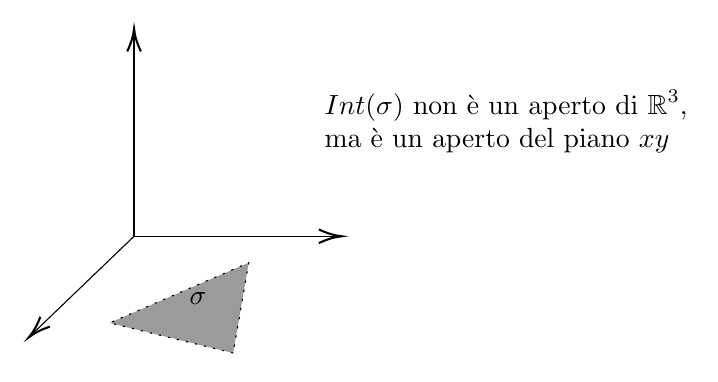
\begin{tikzpicture}[x=0.75pt,y=0.75pt,yscale=-1,xscale=1]
                  %uncomment if require: \path (0,433); %set diagram left start at 0, and has height of 433

                  %Shape: Polygon [id:ds9727174483236036] 
                  \draw  [fill={rgb, 255:red, 155; green, 155; blue, 155 }  ,fill opacity=1 ][dash pattern={on 0.84pt off 2.51pt}] (198.25,176.75) -- (138.75,162.25) -- (205.75,133.25) -- cycle ;
                  %Straight Lines [id:da48881172415233065] 
                  \draw    (150.5,120.5) -- (150.5,22.5) ;
                  \draw [shift={(150.5,20.5)}, rotate = 90] [color={rgb, 255:red, 0; green, 0; blue, 0 }  ][line width=0.75]    (10.93,-3.29) .. controls (6.95,-1.4) and (3.31,-0.3) .. (0,0) .. controls (3.31,0.3) and (6.95,1.4) .. (10.93,3.29)   ;
                  %Shape: Boxed Line [id:dp046526051813471136] 
                  \draw    (150.5,120.5) -- (248.5,120.5) ;
                  \draw [shift={(250.5,120.5)}, rotate = 180] [color={rgb, 255:red, 0; green, 0; blue, 0 }  ][line width=0.75]    (10.93,-3.29) .. controls (6.95,-1.4) and (3.31,-0.3) .. (0,0) .. controls (3.31,0.3) and (6.95,1.4) .. (10.93,3.29)   ;
                  %Straight Lines [id:da07019909443910466] 
                  \draw    (150.5,120.5) -- (101.19,167.86) ;
                  \draw [shift={(99.75,169.25)}, rotate = 316.15] [color={rgb, 255:red, 0; green, 0; blue, 0 }  ][line width=0.75]    (10.93,-3.29) .. controls (6.95,-1.4) and (3.31,-0.3) .. (0,0) .. controls (3.31,0.3) and (6.95,1.4) .. (10.93,3.29)   ;

                  % Text Node
                  \draw (176,146.4) node [anchor=north west][inner sep=0.75pt]    {$\sigma $};
                  % Text Node
                  \draw (241,49) node [anchor=north west][inner sep=0.75pt]   [align=left] {$\displaystyle Int( \sigma )$ non è un aperto di $\displaystyle \mathbb{R}^{3}$,\\ma è un aperto del piano $\displaystyle xy$};


              \end{tikzpicture}

          \end{center}
    \item $\bar{Int(\sigma)}=\sigma$ ossia $Bd(\sigma)$ è la frontiera del simplesso $\sigma$
\end{itemize}
\paragraph{Idea} Non ho una ugualianza, ma posso dire che il k-simplesso è omeomorfo a
\[
    \setst{\underline{x}\in\R^k}{||\underline{x}||\leq 1}
\]
\begin{theorem}
    Sia $U\subseteq\R^n$ un sottoinsieme aperto, connesso, limitato, e sia $P\in U$ un punto. Allora
    \begin{itemize}
        \item Ogni semiretta uscente da $P$ interseca la frontiera $Bd(U)=\bar{U}\setminus U$ esattamente in un punto
        \item C'è un omeomorfismo
              \[
                  \varphi:\bar{U}\ra B_n(1):=\setst{\underline{x}\in\R^n}{||\underline{x}||\leq 1}
              \]
              tale che
              \[
                  \left.\varphi\right|_{Bd(U)}:Bd(U)\ra S^{n-1}:=Bd(B_n(1))
              \]
              è un omeomorfismo tra i due bordi
    \end{itemize}
\end{theorem}
\begin{proof}
    \begin{enumerate}
        \item Sia $r$ una semiretta uscente da $P$ punto del sottoinsieme
              \[
                  r=\setst{\underline{x}\in P+t\underline{v}}{t\geq 0}
              \]
              $r\cap U\subseteq r$ è un sottoinseme aperto di $r$, ed è anche convesso e limitato
              \[
                  r\cap U=\setst{\underline{x}\in P+t\underline{v}}{t\in[0,a)}
              \]
              il punto $Q$ ottenuto come $Q=P+a\underline{v}$ è un punto di frontiera $Q\in Bd(U)=\bar{U}\setminus U$\\
              Devo mostrare che $\{Q\}=r\cap Bd(U)$\\
              Supponiamo che $r$ intersechi il bordo di $U$ anche in un'altro punto $R$\\56
              Il punto $Q$ è compreso tra $P$ e $R$.\\
              \begin{center}


                  \tikzset{every picture/.style={line width=0.75pt}} %set default line width to 0.75pt        

                  \begin{tikzpicture}[x=0.75pt,y=0.75pt,yscale=-1,xscale=1]
                      %uncomment if require: \path (0,433); %set diagram left start at 0, and has height of 433

                      %Shape: Regular Polygon [id:dp5554956992868283] 
                      \draw   (199.98,183.92) .. controls (215.24,173.02) and (242.9,164.82) .. (217.13,95.72) .. controls (191.36,26.61) and (205.67,150.52) .. (173.71,107.45) .. controls (141.74,64.38) and (102.88,156.96) .. (127.03,182.51) .. controls (151.19,208.06) and (184.71,194.82) .. (199.98,183.92) -- cycle ;
                      %Straight Lines [id:da581561872364778] 
                      \draw    (149.5,140.25) -- (205.5,90.75) ;
                      \draw [shift={(205.5,90.75)}, rotate = 318.53] [color={rgb, 255:red, 0; green, 0; blue, 0 }  ][fill={rgb, 255:red, 0; green, 0; blue, 0 }  ][line width=0.75]      (0, 0) circle [x radius= 3.35, y radius= 3.35]   ;
                      \draw [shift={(149.5,140.25)}, rotate = 318.53] [color={rgb, 255:red, 0; green, 0; blue, 0 }  ][fill={rgb, 255:red, 0; green, 0; blue, 0 }  ][line width=0.75]      (0, 0) circle [x radius= 3.35, y radius= 3.35]   ;

                      % Text Node
                      \draw (136,148.9) node [anchor=north west][inner sep=0.75pt]    {$P$};
                      % Text Node
                      \draw (215,68.65) node [anchor=north west][inner sep=0.75pt]    {$R$};
                      % Text Node
                      \draw (282.5,80) node [anchor=north west][inner sep=0.75pt]   [align=left] {Non è più connesso};


                  \end{tikzpicture}

              \end{center}
              In coordinate $R=P+b\underline{v}$ con $b>a$\\
              Quali sono le coordinate baricentriche di $Q$ rispetto all'1-simplesso generato da $P$ e $R$?
              \[
                  Q=t_0R+t_1P\quad\quad t_0+t_1=1
              \]
              \[
                  Q=(1-t)R+tP
              \]
              \[
                  Q=P+a\underline{v}
              \]
              \[
                  b\underline{v}=R-P
              \]
              \[
                  a\underline{v}=\frac{a}{b}b\underline{v}=\frac{a}{b}R-P
              \]
              da cui
              \[
                  Q=P+\frac{a}{b}R-\frac{a}{b}P=\left(1-\frac{a}{b}\right)P+\frac{a}{b}R
              \]
              esplicitando P
              \[
                  bQ=(b-a)P+aR\longleftrightarrow P=\frac{1}{b-a}(bQ-aR)
              \]
              $R\in Bd(U)$ sse esiste una successione di punti $\{R_N\}_{N\in\N}$ tale che
              \[
                  R_N\in U,\quad \text{ma } \lim_{n\ra+\infty}R_N=R
              \]
              Vado a sostituire i punti $R_N$ nella relazione che definisce $P$ in funzione di $Q$ e $R$
              \[
                  P_N=\frac{1}{b-a}(bQ-aR_N)
              \]
              %IMMAGINE%
              Per ipotesi, $U$ è aperto, quindi esiste un valore $N_0\in\N$ tale che
              \[
                  \forall N\geq N_0,\quad P_N\in U
              \]
              Per $N\geq N_0$, $P_N$ e $R_N\in U$.\\
              $U$ è connesso, $Q\in U$ ($Q$ unione di $R_N$ e $P_N$)\\
              Contraddizione, poichè per itpotesi $Q\in Bd(U)$\\
              \[
                  R\neq q\in Bd(U)
              \]
              non può esistere
        \item A meno di traslazioni, posso supporre che $P\in U$ $P=\underline{0}$\\
              Considero la funzione $f:\R^n\setminus\{\underline{0}\}\ra S^{n-1}$ definita da
              \[
                  \underline{x}\mapsto\frac{\underline{x}}{||\underline{x}||}
              \]
              Ogni semiretta passante per l'origine, interseca sia $S^{n-1}$ che il bordo $Bd(U)$ in un unico punto
              \[
                  \left.f\right|_{Bd(U)}:Bd(U)\ra S^{n-1}
              \]
              $f$ è biettiva, quindi $\left.f\right|_{Bd(U)}$ è un omeomorfismo tra $Bd(U)$ e $Bd(B_n(1))=S^{n-1}$\\
              Sia $g:S^{n-1}\ra Bd(u)$ la funzione inversa di $f$.\\
              Voglio estendere $g$ ad una funzione $\bar{g}:B_n(1)\ra U$\\
              L'idea è di dilatare/contrarre ogni segmento di estremi $\underline{0}$ e $\underline{y}$ nel segmento di estremi $\underline{0}$ e $g(\underline{y})$\\
              $\forall Q\in B_n(1)$ $Q=t\underline{v}$ con $\underline{v}$ versore, quindi $t\in(0,1]$\\
              Il segmento tra $\underline{0}$ e $\frac{Q}{||Q||}$ viene mandato nel segmento tra $\underline{0}$ e $g\left(\frac{Q}{||Q||}\right)$\\
              Il fattore di scala è dato da
              \[
                  \left|\left|g\left(\frac{Q}{||Q||}\right)\right|\right|
              \]
              quindi $Q=t\underline{v}$ viene mandato in
              \[t\left|\left|g\left(\frac{Q}{||Q||}\right)\right|\right|\underline{v}\]
              $\bar{g}:B_n(1)\ra U$ è definito da
              \[
                  \bar{g}(z)=\left\{
                  \begin{array}{ll}
                      (0,\dots,0)                                              & z=\underline{0}    \\
                      \left|\left|g\left(\frac{Q}{||Q||}\right)\right|\right|z & z\neq\underline{0}
                  \end{array}
                  \right.
              \]
              $\bar{g}$ è invertibile ed è continua sicuramente per $z\neq\underline{0}$.\\
              Cosa posso dire di $\underline{0}$? Osservo che
              \[
                  ||g||:S^{n-1}\ra\R
              \]
              definita da $||g||(x)=||g(x)||$ è limitata, quindi posso prendeer $M=\max_{S^{n-1}}||g||$
              \[
                  0\leq||z-\underline{0}||\leq\delta\implies||\bar{g}(z)-g(\underline{0})||<M\delta
              \]
              $\bar{g}$ è continua anche in $\underline{0}$
    \end{enumerate}
\end{proof}
\paragraph{Per riassumere} Dal punto di vista topologico, i k-simplessi di $\R^n$ ha le stesse proprietà di una palla n-dimensionale.\\
Dal punto di vista metrico invece, le proprietà sono molto diverse, ad esempio l'area contenuta è diversa
\chapter{Complessi simpliciali}
Una domanda sorge spontanea: Posso utilizzare i simplessi per approssimare una forma qualsiasi
\begin{center}


    \tikzset{every picture/.style={line width=0.75pt}} %set default line width to 0.75pt        

    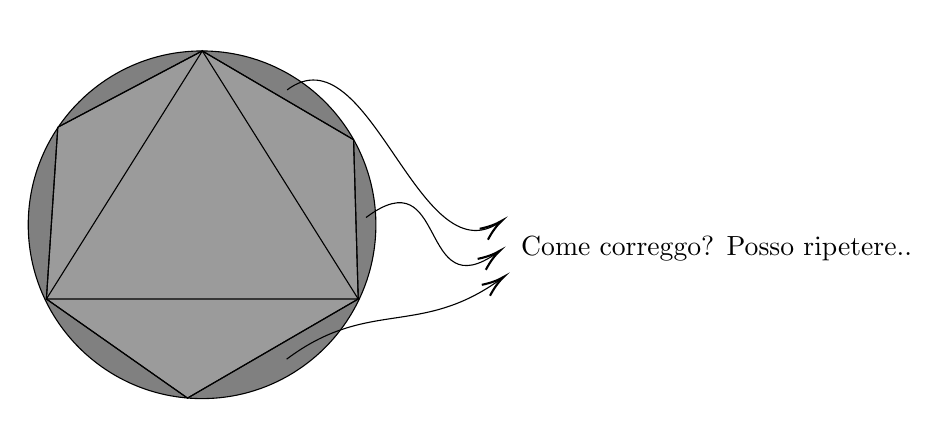
\begin{tikzpicture}[x=0.75pt,y=0.75pt,yscale=-1,xscale=1]
        %uncomment if require: \path (0,433); %set diagram left start at 0, and has height of 433

        %Shape: Circle [id:dp9315706344783725] 
        \draw  [fill={rgb, 255:red, 128; green, 128; blue, 128 }  ,fill opacity=1 ] (91,102.75) .. controls (91,56.5) and (128.5,19) .. (174.75,19) .. controls (221,19) and (258.5,56.5) .. (258.5,102.75) .. controls (258.5,149) and (221,186.5) .. (174.75,186.5) .. controls (128.5,186.5) and (91,149) .. (91,102.75) -- cycle ;
        %Shape: Polygon [id:ds441065514005603] 
        \draw  [fill={rgb, 255:red, 155; green, 155; blue, 155 }  ,fill opacity=1 ] (105.25,55.75) -- (174.88,19) -- (247.75,61.75) -- (250,138.5) -- (167.75,186.25) -- (99.75,138.5) -- cycle ;
        %Shape: Triangle [id:dp10410292750489414] 
        \draw  [fill={rgb, 255:red, 155; green, 155; blue, 155 }  ,fill opacity=1 ] (174.88,19) -- (250,138.5) -- (99.75,138.5) -- cycle ;
        %Straight Lines [id:da6589061007004249] 
        \draw    (99.75,138.5) -- (105.25,55.75) ;
        %Straight Lines [id:da5829781694864387] 
        \draw    (105.25,55.75) -- (174.75,19) ;
        %Straight Lines [id:da9920223672264377] 
        \draw    (99.75,138.5) -- (167.75,186.25) -- (250,138.5) ;
        %Straight Lines [id:da12856023583957388] 
        \draw    (250,138.5) -- (247.75,61.75) -- (174.88,19) ;
        %Curve Lines [id:da7391701293373687] 
        \draw    (215.5,167.5) .. controls (255.1,137.8) and (279.75,157.35) .. (319.05,128.64) ;
        \draw [shift={(320.25,127.75)}, rotate = 143.13] [color={rgb, 255:red, 0; green, 0; blue, 0 }  ][line width=0.75]    (10.93,-3.29) .. controls (6.95,-1.4) and (3.31,-0.3) .. (0,0) .. controls (3.31,0.3) and (6.95,1.4) .. (10.93,3.29)   ;
        %Curve Lines [id:da33478284879748066] 
        \draw    (253.75,99.25) .. controls (293.35,69.55) and (278.55,143.74) .. (317.07,116.12) ;
        \draw [shift={(318.25,115.25)}, rotate = 143.13] [color={rgb, 255:red, 0; green, 0; blue, 0 }  ][line width=0.75]    (10.93,-3.29) .. controls (6.95,-1.4) and (3.31,-0.3) .. (0,0) .. controls (3.31,0.3) and (6.95,1.4) .. (10.93,3.29)   ;
        %Curve Lines [id:da15996388909968506] 
        \draw    (215.75,37.75) .. controls (255.35,8.05) and (278.78,128.31) .. (318.05,101.6) ;
        \draw [shift={(319.25,100.75)}, rotate = 143.13] [color={rgb, 255:red, 0; green, 0; blue, 0 }  ][line width=0.75]    (10.93,-3.29) .. controls (6.95,-1.4) and (3.31,-0.3) .. (0,0) .. controls (3.31,0.3) and (6.95,1.4) .. (10.93,3.29)   ;

        % Text Node
        \draw (327.25,107) node [anchor=north west][inner sep=0.75pt]   [align=left] {Come correggo? Posso ripetere..};


    \end{tikzpicture}

\end{center}
\begin{definition}[Complesso simpliciale]
    Un complesso simpliciale (simplicial complex) $K$ di $\R^n$ è una collezione di simplessi tali che
    \begin{enumerate}
        \item Ogni faccia di un simplesso di $K$ appartiene a $K$
        \item L'intersezione di due simplessi di $K$ è una faccia di entrambi, oppure è vuota
    \end{enumerate}
\end{definition}
\paragraph{Esempio 1}
Consideriamo il simplesso $\sigma=[P_0,P_1,P_2]$ generato da $\{P_0,P_1,P_2\}$
\begin{center}


    \tikzset{every picture/.style={line width=0.75pt}} %set default line width to 0.75pt        

    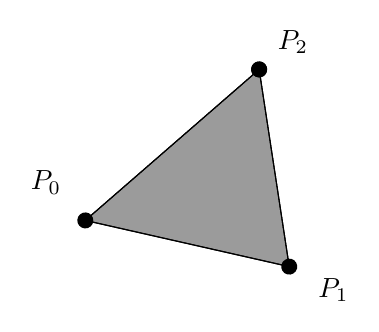
\begin{tikzpicture}[x=0.75pt,y=0.75pt,yscale=-1,xscale=1]
        %uncomment if require: \path (0,433); %set diagram left start at 0, and has height of 433

        %Shape: Polygon [id:ds41744765568909314] 
        \draw  [fill={rgb, 255:red, 155; green, 155; blue, 155 }  ,fill opacity=1 ] (198.25,143.25) -- (100,121) -- (183.75,48.25) -- cycle ;
        %Straight Lines [id:da4521438473956243] 
        \draw    (100,121) -- (183.75,48.25) ;
        \draw [shift={(183.75,48.25)}, rotate = 319.02] [color={rgb, 255:red, 0; green, 0; blue, 0 }  ][fill={rgb, 255:red, 0; green, 0; blue, 0 }  ][line width=0.75]      (0, 0) circle [x radius= 3.35, y radius= 3.35]   ;
        \draw [shift={(100,121)}, rotate = 319.02] [color={rgb, 255:red, 0; green, 0; blue, 0 }  ][fill={rgb, 255:red, 0; green, 0; blue, 0 }  ][line width=0.75]      (0, 0) circle [x radius= 3.35, y radius= 3.35]   ;
        %Straight Lines [id:da9366118076239045] 
        \draw    (198.25,143.25) -- (183.75,48.25) ;
        \draw [shift={(183.75,48.25)}, rotate = 261.32] [color={rgb, 255:red, 0; green, 0; blue, 0 }  ][fill={rgb, 255:red, 0; green, 0; blue, 0 }  ][line width=0.75]      (0, 0) circle [x radius= 3.35, y radius= 3.35]   ;
        \draw [shift={(198.25,143.25)}, rotate = 261.32] [color={rgb, 255:red, 0; green, 0; blue, 0 }  ][fill={rgb, 255:red, 0; green, 0; blue, 0 }  ][line width=0.75]      (0, 0) circle [x radius= 3.35, y radius= 3.35]   ;
        %Straight Lines [id:da2058216992161228] 
        \draw    (100,121) -- (198.25,143.25) ;

        % Text Node
        \draw (72.5,95.9) node [anchor=north west][inner sep=0.75pt]    {$P_{0}$};
        % Text Node
        \draw (211,147.9) node [anchor=north west][inner sep=0.75pt]    {$P_{1}$};
        % Text Node
        \draw (191.5,28.4) node [anchor=north west][inner sep=0.75pt]    {$P_{2}$};


    \end{tikzpicture}

\end{center}
$K=\{\sigma\}$ non è un complesso simpliciale poichè non rispetta la prima regola. Il più piccolo complesso simpliciale che contiene $\sigma$ è la collezione
\[
    K=\{\sigma,\underbrace{[P_0,P_1],[P_0,P_2],[P_1,P_2]}_{1-simplessi},\underbrace{[P_0],[P_1],[P_2]}_{0-simplessi}\}
\]
\paragraph{Esempio 2}
\begin{center}


    \tikzset{every picture/.style={line width=0.75pt}} %set default line width to 0.75pt        

    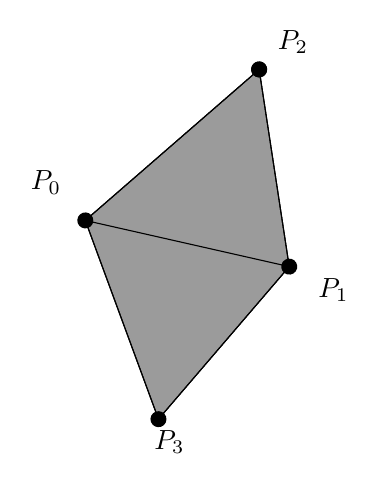
\begin{tikzpicture}[x=0.75pt,y=0.75pt,yscale=-1,xscale=1]
        %uncomment if require: \path (0,433); %set diagram left start at 0, and has height of 433

        %Shape: Polygon [id:ds41744765568909314] 
        \draw  [fill={rgb, 255:red, 155; green, 155; blue, 155 }  ,fill opacity=1 ] (135.25,216.75) -- (100,121) -- (183.75,48.25) -- (198.25,143.25) -- cycle ;
        %Straight Lines [id:da4521438473956243] 
        \draw    (100,121) -- (183.75,48.25) ;
        \draw [shift={(183.75,48.25)}, rotate = 319.02] [color={rgb, 255:red, 0; green, 0; blue, 0 }  ][fill={rgb, 255:red, 0; green, 0; blue, 0 }  ][line width=0.75]      (0, 0) circle [x radius= 3.35, y radius= 3.35]   ;
        \draw [shift={(100,121)}, rotate = 319.02] [color={rgb, 255:red, 0; green, 0; blue, 0 }  ][fill={rgb, 255:red, 0; green, 0; blue, 0 }  ][line width=0.75]      (0, 0) circle [x radius= 3.35, y radius= 3.35]   ;
        %Straight Lines [id:da9366118076239045] 
        \draw    (198.25,143.25) -- (183.75,48.25) ;
        \draw [shift={(183.75,48.25)}, rotate = 261.32] [color={rgb, 255:red, 0; green, 0; blue, 0 }  ][fill={rgb, 255:red, 0; green, 0; blue, 0 }  ][line width=0.75]      (0, 0) circle [x radius= 3.35, y radius= 3.35]   ;
        \draw [shift={(198.25,143.25)}, rotate = 261.32] [color={rgb, 255:red, 0; green, 0; blue, 0 }  ][fill={rgb, 255:red, 0; green, 0; blue, 0 }  ][line width=0.75]      (0, 0) circle [x radius= 3.35, y radius= 3.35]   ;
        %Straight Lines [id:da2058216992161228] 
        \draw    (100,121) -- (198.25,143.25) ;
        %Straight Lines [id:da3469509626744045] 
        \draw    (100,121) -- (135.25,216.75) ;
        \draw [shift={(135.25,216.75)}, rotate = 69.79] [color={rgb, 255:red, 0; green, 0; blue, 0 }  ][fill={rgb, 255:red, 0; green, 0; blue, 0 }  ][line width=0.75]      (0, 0) circle [x radius= 3.35, y radius= 3.35]   ;
        %Straight Lines [id:da09585082925168376] 
        \draw    (198.25,143.25) -- (135.25,216.75) ;

        % Text Node
        \draw (72.5,95.9) node [anchor=north west][inner sep=0.75pt]    {$P_{0}$};
        % Text Node
        \draw (211,147.9) node [anchor=north west][inner sep=0.75pt]    {$P_{1}$};
        % Text Node
        \draw (191.5,28.4) node [anchor=north west][inner sep=0.75pt]    {$P_{2}$};
        % Text Node
        \draw (132,220.9) node [anchor=north west][inner sep=0.75pt]    {$P_{3}$};


    \end{tikzpicture}

\end{center}
\[
    K=\left\{
    \begin{array}{ll}
        {[P_0,P_1,P_2],[P_0,P_1,P_3],}                       \\
        {[P_0,P_1],[P_1,P_2],[P_0,P_2],[P_0,P_3],[P_1,P_3],} \\
        {[P_0],[P_1],[P_2],[P_3]}
    \end{array}\right\}
\]
\paragraph{Esempio 3}
\begin{center}


    \tikzset{every picture/.style={line width=0.75pt}} %set default line width to 0.75pt        

    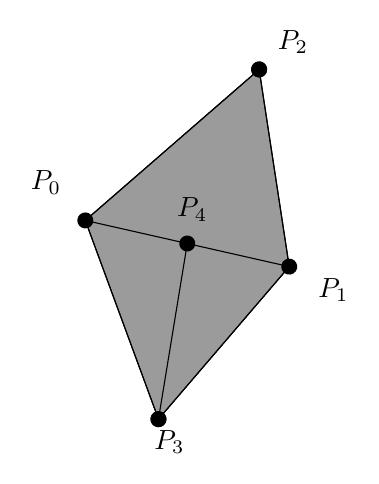
\begin{tikzpicture}[x=0.75pt,y=0.75pt,yscale=-1,xscale=1]
        %uncomment if require: \path (0,433); %set diagram left start at 0, and has height of 433

        %Shape: Polygon [id:ds41744765568909314] 
        \draw  [fill={rgb, 255:red, 155; green, 155; blue, 155 }  ,fill opacity=1 ] (135.25,216.75) -- (100,121) -- (183.75,48.25) -- (198.25,143.25) -- cycle ;
        %Straight Lines [id:da4521438473956243] 
        \draw    (100,121) -- (183.75,48.25) ;
        \draw [shift={(183.75,48.25)}, rotate = 319.02] [color={rgb, 255:red, 0; green, 0; blue, 0 }  ][fill={rgb, 255:red, 0; green, 0; blue, 0 }  ][line width=0.75]      (0, 0) circle [x radius= 3.35, y radius= 3.35]   ;
        \draw [shift={(100,121)}, rotate = 319.02] [color={rgb, 255:red, 0; green, 0; blue, 0 }  ][fill={rgb, 255:red, 0; green, 0; blue, 0 }  ][line width=0.75]      (0, 0) circle [x radius= 3.35, y radius= 3.35]   ;
        %Straight Lines [id:da9366118076239045] 
        \draw    (198.25,143.25) -- (183.75,48.25) ;
        \draw [shift={(183.75,48.25)}, rotate = 261.32] [color={rgb, 255:red, 0; green, 0; blue, 0 }  ][fill={rgb, 255:red, 0; green, 0; blue, 0 }  ][line width=0.75]      (0, 0) circle [x radius= 3.35, y radius= 3.35]   ;
        \draw [shift={(198.25,143.25)}, rotate = 261.32] [color={rgb, 255:red, 0; green, 0; blue, 0 }  ][fill={rgb, 255:red, 0; green, 0; blue, 0 }  ][line width=0.75]      (0, 0) circle [x radius= 3.35, y radius= 3.35]   ;
        %Straight Lines [id:da2058216992161228] 
        \draw    (100,121) -- (198.25,143.25) ;
        %Straight Lines [id:da3469509626744045] 
        \draw    (100,121) -- (135.25,216.75) ;
        \draw [shift={(135.25,216.75)}, rotate = 69.79] [color={rgb, 255:red, 0; green, 0; blue, 0 }  ][fill={rgb, 255:red, 0; green, 0; blue, 0 }  ][line width=0.75]      (0, 0) circle [x radius= 3.35, y radius= 3.35]   ;
        %Straight Lines [id:da09585082925168376] 
        \draw    (198.25,143.25) -- (135.25,216.75) ;
        %Straight Lines [id:da8259875281713551] 
        \draw    (149.13,132.13) -- (135.25,216.75) ;
        \draw [shift={(135.25,216.75)}, rotate = 99.31] [color={rgb, 255:red, 0; green, 0; blue, 0 }  ][fill={rgb, 255:red, 0; green, 0; blue, 0 }  ][line width=0.75]      (0, 0) circle [x radius= 3.35, y radius= 3.35]   ;
        \draw [shift={(149.13,132.13)}, rotate = 99.31] [color={rgb, 255:red, 0; green, 0; blue, 0 }  ][fill={rgb, 255:red, 0; green, 0; blue, 0 }  ][line width=0.75]      (0, 0) circle [x radius= 3.35, y radius= 3.35]   ;

        % Text Node
        \draw (72.5,95.9) node [anchor=north west][inner sep=0.75pt]    {$P_{0}$};
        % Text Node
        \draw (211,147.9) node [anchor=north west][inner sep=0.75pt]    {$P_{1}$};
        % Text Node
        \draw (191.5,28.4) node [anchor=north west][inner sep=0.75pt]    {$P_{2}$};
        % Text Node
        \draw (132,220.9) node [anchor=north west][inner sep=0.75pt]    {$P_{3}$};
        % Text Node
        \draw (143,108.9) node [anchor=north west][inner sep=0.75pt]    {$P_{4}$};


    \end{tikzpicture}

\end{center}
Non è un complesso simpliciale, infatti
\[
    [P_0,P_1,P_2]\cap[P_0,P_3,P_4]=[P_0,P_4]
\]
non è una faccia di $[P_0,P_1,P_2]$
\begin{lemma}
    Condizione equivalente per essere un complesso simpliciale:\\
    Una collezione $K$ di simplessi di $\R^n$ è un complesso simpliciale se:
    \begin{itemize}
        \item Ogni faccia di un simplesso di $K$ appartiene a $K$
        \item Due simplessi distinti hanno interno disgiunto
              \[
                  \sigma\neq\tau,\quad Int(\sigma)\cap Int(\tau)=\emptyset,\quad \forall\sigma,\tau\in K
              \]
    \end{itemize}
\end{lemma}
\paragraph{Nell'esempio}
\[
    [P_0,P_1]\neq[P_0,P_4]
\]
ma
\[
    Int([P_0,P_1])\cap Int([P_0,P_4])=Int([P_0,P_4])\neq\emptyset
\]
\begin{definition}[Sottocomplesso simpliciale]
    Sia $K$ un complesso simpliciale, una collezione $L$ di simplessi di $K$ che contiene anche le facce di tutti i suoi elementi è ancora un complesso simpliciale.\\
    Diciamo che $L$ è un sottocomplesso di $K$
\end{definition}
\begin{definition}[P-scheletro]
    Dato un complesso simpliciale $K$, definiamo p-scheletro di $K$ il sottocomplesso
    \[
        K^{(p)}:=\setst{\sigma\in K}{dim\ \sigma\leq p}
    \]˜
\end{definition}
\begin{definition}[Dimensione di un complesso]
    Dato un complesso simpliciale $K$, chiamiamo dimensione di $K$ il numero
    \[
        dim\ K=\max_{\sigma\in K}(dim\ \sigma)
    \]
\end{definition}
\paragraph{Osservazione} In particolare, lo 0-scheletro è l'insieme dei vertici e ogni scheletro
\[
    K^{(0)}\subseteq K^{(1)}\subseteq K^{(2)}\subseteq\dots\subseteq K^{(dim\ K)}=K
\]
\begin{center}


    \tikzset{every picture/.style={line width=0.75pt}} %set default line width to 0.75pt        

    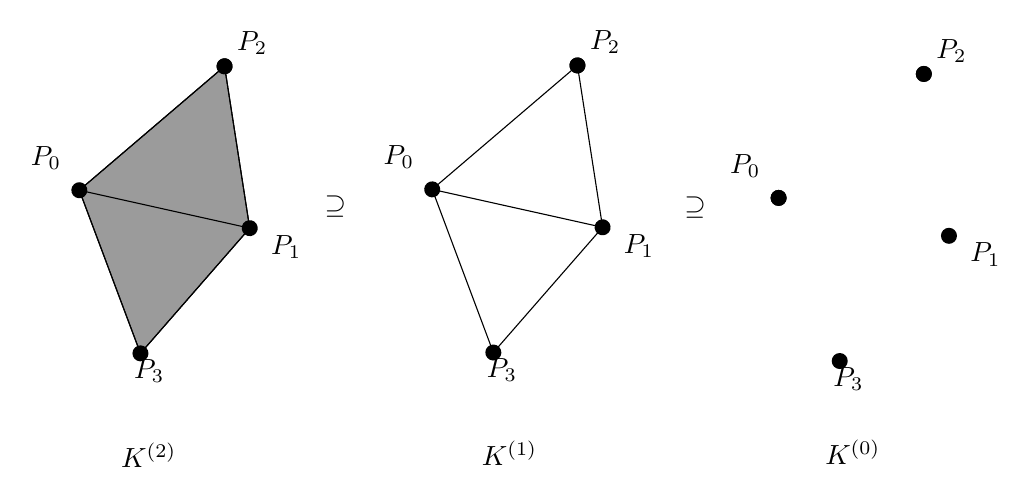
\begin{tikzpicture}[x=0.75pt,y=0.75pt,yscale=-1,xscale=1]
        %uncomment if require: \path (0,433); %set diagram left start at 0, and has height of 433

        %Shape: Polygon [id:ds41744765568909314] 
        \draw  [fill={rgb, 255:red, 155; green, 155; blue, 155 }  ,fill opacity=1 ] (65.26,167.99) -- (35.81,89.39) -- (105.78,29.67) -- (117.9,107.66) -- cycle ;
        %Straight Lines [id:da4521438473956243] 
        \draw    (35.81,89.39) -- (105.78,29.67) ;
        \draw [shift={(105.78,29.67)}, rotate = 319.52] [color={rgb, 255:red, 0; green, 0; blue, 0 }  ][fill={rgb, 255:red, 0; green, 0; blue, 0 }  ][line width=0.75]      (0, 0) circle [x radius= 3.35, y radius= 3.35]   ;
        \draw [shift={(35.81,89.39)}, rotate = 319.52] [color={rgb, 255:red, 0; green, 0; blue, 0 }  ][fill={rgb, 255:red, 0; green, 0; blue, 0 }  ][line width=0.75]      (0, 0) circle [x radius= 3.35, y radius= 3.35]   ;
        %Straight Lines [id:da9366118076239045] 
        \draw    (117.9,107.66) -- (105.78,29.67) ;
        \draw [shift={(105.78,29.67)}, rotate = 261.17] [color={rgb, 255:red, 0; green, 0; blue, 0 }  ][fill={rgb, 255:red, 0; green, 0; blue, 0 }  ][line width=0.75]      (0, 0) circle [x radius= 3.35, y radius= 3.35]   ;
        \draw [shift={(117.9,107.66)}, rotate = 261.17] [color={rgb, 255:red, 0; green, 0; blue, 0 }  ][fill={rgb, 255:red, 0; green, 0; blue, 0 }  ][line width=0.75]      (0, 0) circle [x radius= 3.35, y radius= 3.35]   ;
        %Straight Lines [id:da2058216992161228] 
        \draw    (35.81,89.39) -- (117.9,107.66) ;
        %Straight Lines [id:da3469509626744045] 
        \draw    (35.81,89.39) -- (65.26,167.99) ;
        \draw [shift={(65.26,167.99)}, rotate = 69.46] [color={rgb, 255:red, 0; green, 0; blue, 0 }  ][fill={rgb, 255:red, 0; green, 0; blue, 0 }  ][line width=0.75]      (0, 0) circle [x radius= 3.35, y radius= 3.35]   ;
        %Straight Lines [id:da09585082925168376] 
        \draw    (117.9,107.66) -- (65.26,167.99) ;
        %Straight Lines [id:da08247903260298006] 
        \draw    (205.83,88.98) -- (275.8,29.26) ;
        \draw [shift={(275.8,29.26)}, rotate = 319.52] [color={rgb, 255:red, 0; green, 0; blue, 0 }  ][fill={rgb, 255:red, 0; green, 0; blue, 0 }  ][line width=0.75]      (0, 0) circle [x radius= 3.35, y radius= 3.35]   ;
        \draw [shift={(205.83,88.98)}, rotate = 319.52] [color={rgb, 255:red, 0; green, 0; blue, 0 }  ][fill={rgb, 255:red, 0; green, 0; blue, 0 }  ][line width=0.75]      (0, 0) circle [x radius= 3.35, y radius= 3.35]   ;
        %Straight Lines [id:da14894457440526065] 
        \draw    (287.92,107.25) -- (275.8,29.26) ;
        \draw [shift={(275.8,29.26)}, rotate = 261.17] [color={rgb, 255:red, 0; green, 0; blue, 0 }  ][fill={rgb, 255:red, 0; green, 0; blue, 0 }  ][line width=0.75]      (0, 0) circle [x radius= 3.35, y radius= 3.35]   ;
        \draw [shift={(287.92,107.25)}, rotate = 261.17] [color={rgb, 255:red, 0; green, 0; blue, 0 }  ][fill={rgb, 255:red, 0; green, 0; blue, 0 }  ][line width=0.75]      (0, 0) circle [x radius= 3.35, y radius= 3.35]   ;
        %Straight Lines [id:da8315514213699629] 
        \draw    (205.83,88.98) -- (287.92,107.25) ;
        %Straight Lines [id:da9223671103273994] 
        \draw    (205.83,88.98) -- (235.28,167.58) ;
        \draw [shift={(235.28,167.58)}, rotate = 69.46] [color={rgb, 255:red, 0; green, 0; blue, 0 }  ][fill={rgb, 255:red, 0; green, 0; blue, 0 }  ][line width=0.75]      (0, 0) circle [x radius= 3.35, y radius= 3.35]   ;
        %Straight Lines [id:da9641539818005227] 
        \draw    (287.92,107.25) -- (235.28,167.58) ;
        %Straight Lines [id:da3412338985513719] 
        \draw    (372.72,93.09) ;
        \draw [shift={(372.72,93.09)}, rotate = 0] [color={rgb, 255:red, 0; green, 0; blue, 0 }  ][fill={rgb, 255:red, 0; green, 0; blue, 0 }  ][line width=0.75]      (0, 0) circle [x radius= 3.35, y radius= 3.35]   ;
        \draw [shift={(372.72,93.09)}, rotate = 0] [color={rgb, 255:red, 0; green, 0; blue, 0 }  ][fill={rgb, 255:red, 0; green, 0; blue, 0 }  ][line width=0.75]      (0, 0) circle [x radius= 3.35, y radius= 3.35]   ;
        %Straight Lines [id:da09923500544570385] 
        \draw    (442.69,33.37) ;
        \draw [shift={(442.69,33.37)}, rotate = 0] [color={rgb, 255:red, 0; green, 0; blue, 0 }  ][fill={rgb, 255:red, 0; green, 0; blue, 0 }  ][line width=0.75]      (0, 0) circle [x radius= 3.35, y radius= 3.35]   ;
        \draw [shift={(442.69,33.37)}, rotate = 0] [color={rgb, 255:red, 0; green, 0; blue, 0 }  ][fill={rgb, 255:red, 0; green, 0; blue, 0 }  ][line width=0.75]      (0, 0) circle [x radius= 3.35, y radius= 3.35]   ;
        %Straight Lines [id:da2978154430200619] 
        \draw    (454.8,111.35) ;
        \draw [shift={(454.8,111.35)}, rotate = 0] [color={rgb, 255:red, 0; green, 0; blue, 0 }  ][fill={rgb, 255:red, 0; green, 0; blue, 0 }  ][line width=0.75]      (0, 0) circle [x radius= 3.35, y radius= 3.35]   ;
        %Straight Lines [id:da7158042054580731] 
        \draw    (402.17,171.68) ;
        \draw [shift={(402.17,171.68)}, rotate = 0] [color={rgb, 255:red, 0; green, 0; blue, 0 }  ][fill={rgb, 255:red, 0; green, 0; blue, 0 }  ][line width=0.75]      (0, 0) circle [x radius= 3.35, y radius= 3.35]   ;
        %Straight Lines [id:da106514796744958] 
        \draw    (454.8,111.35) ;

        % Text Node
        \draw (11.19,67.16) node [anchor=north west][inner sep=0.75pt]    {$P_{0}$};
        % Text Node
        \draw (126.9,109.84) node [anchor=north west][inner sep=0.75pt]    {$P_{1}$};
        % Text Node
        \draw (110.61,11.75) node [anchor=north west][inner sep=0.75pt]    {$P_{2}$};
        % Text Node
        \draw (60.9,169.76) node [anchor=north west][inner sep=0.75pt]    {$P_{3}$};
        % Text Node
        \draw (181.21,66.75) node [anchor=north west][inner sep=0.75pt]    {$P_{0}$};
        % Text Node
        \draw (296.92,109.43) node [anchor=north west][inner sep=0.75pt]    {$P_{1}$};
        % Text Node
        \draw (280.63,11.34) node [anchor=north west][inner sep=0.75pt]    {$P_{2}$};
        % Text Node
        \draw (230.92,169.35) node [anchor=north west][inner sep=0.75pt]    {$P_{3}$};
        % Text Node
        \draw (348.1,70.85) node [anchor=north west][inner sep=0.75pt]    {$P_{0}$};
        % Text Node
        \draw (463.81,113.54) node [anchor=north west][inner sep=0.75pt]    {$P_{1}$};
        % Text Node
        \draw (447.52,15.44) node [anchor=north west][inner sep=0.75pt]    {$P_{2}$};
        % Text Node
        \draw (397.81,173.46) node [anchor=north west][inner sep=0.75pt]    {$P_{3}$};
        % Text Node
        \draw (152.68,90.73) node [anchor=north east][inner sep=0.75pt]  [xscale=-1]  {$\subseteq $};
        % Text Node
        \draw (326.04,91.55) node [anchor=north east][inner sep=0.75pt]  [xscale=-1]  {$\subseteq $};
        % Text Node
        \draw (54.73,209.87) node [anchor=north west][inner sep=0.75pt]    {$K^{( 2)}$};
        % Text Node
        \draw (228.51,209.05) node [anchor=north west][inner sep=0.75pt]    {$K^{( 1)}$};
        % Text Node
        \draw (393.93,208.64) node [anchor=north west][inner sep=0.75pt]    {$K^{( 0)}$};


    \end{tikzpicture}

\end{center}
\begin{definition}[Spazio soggiacente]
    Sia $K$ un complesso simpliciale di $\R^n$, indichiamo con $|K|$ il sottoinsieme $\R^n$ formato dall'unione di punti contenuti nei simplessi di $K$, e lo chiameremo spazio soggiacente di $K$ (o politopo / poliedro di $K$)
\end{definition}
\begin{definition}[Topologia del complesso]
    Dato lo spazio soggiacente, la topologia è definita dai chiusi seguenti:
    \[
        A\subset|K|\ \text{insieme chiuso di }|K|\Longleftrightarrow A\cap\sigma\ \text{insieme chiuso di }\sigma\quad\forall\sigma\in K
    \]
\end{definition}
\paragraph{Nota bene} Alcuni testi utilizzano politopo per indicare lo spazio soggiacente solo nel caso in cui $K$ sia una collezione finita
\begin{proposition}
    Se $K$ è una collezione finita, la topologia del complesso coincide con la topologia euclidea. In generale, la topologia indotta dal complesso simpliciale è più fine della topologia indotta dalla topologia euclidea di $\R^n$ (ho più chiusi / aperti)
\end{proposition}
\paragraph{Osservazione} Se $L$ è un sottocomplesso di $K$, allora lo spazio soggiacente di $|L|$ è un chiuso dello spazio soggiacente di $|K|$.\\
In particolare
\[
    \forall\sigma\in K\quad |\sigma|\ chiuso
\]
infatti
\[
    \forall\sigma\in K\quad |L|\cap\sigma=\left\{\begin{array}{ll}
        \emptyset & \sigma\notin L \\
        \sigma    & \sigma\in L
    \end{array} \right.
\]
\begin{lemma}
    Sia $K$ complesso simpliciale,
    \begin{itemize}
        \item Se $K$ è una collezione finita, allora $|K|$ è compatto
        \item Se $A\subset|K|$ compatto, allora esiste un sottocomplesso $K_0$ finito tale che
              \[
                  A=|L_0K
              \]
    \end{itemize}
\end{lemma}
\paragraph{Osservazione} Se $K$ è una collezione finita, allora la topologia è quella euclidea, e ogni elemento $\sigma$ di $K$ è compatto, quindi $K$ è unione finita di compatti, ossia $|K|$ è compatto
\begin{proposition}
    Una funzione
    \[
        f:|K|\ra X
    \]
    è continua se e solo se
    \[
        \left.f\right|_\sigma:\sigma\ra X
    \]
    è continua $\forall\sigma\in K$
\end{proposition}
\begin{proof}
    $f$ continua se e solo se
    \[
        \forall C\subset X\text{ chiuso, } f^{-1}(C)\text{ è un chiuso di }|K|
    \]
    \begin{itemize}
        \item [$\implies$)] $f:|K|\ra X$ continua. $\left.f\right|_\sigma:\sigma\ra X$ è continua poichè $\sigma$ è un chiuso di $|K|$
        \item [$\impliedby$)] $C\subset X$ chiuso, $\left.f\right|_\sigma:\sigma\ra X$ continua $\forall\sigma\in K$. Per ipotesi, $\left.f^{-1}\right|_\sigma(C)$ è un chiuso (poichè continua), e $\left.f^{-1}\right|_\sigma(C)=f^{-1}(C)\cap\sigma$, chiuso $\forall\sigma\in K$.\\
              $f^{-1}(C)\cap\sigma$ è chiuso $\forall\sigma\in K$, quindi $f^{-1}(C)$ è un chiuso di $|K|$ per definizione di chiuso, quindi $f$ è continua
    \end{itemize}
\end{proof}
\chapter{Sottospazi particolari di un poliedro}
Sia $K$ un complesso simpliciale
\begin{definition}[Star di un vertice]
    Per ogni vertice $v\in K^{(0)}$, definiamo star di $v$ l'unione della parte interna di tutti i simplessi di $K$ che hanno $v$ come vertice, ossia
    \[
        St(v)=St(v,K)=\bigsqcup_{v\in\sigma\in K}Int(\sigma)
    \]
\end{definition}
\begin{center}


    \tikzset{every picture/.style={line width=0.75pt}} %set default line width to 0.75pt        

    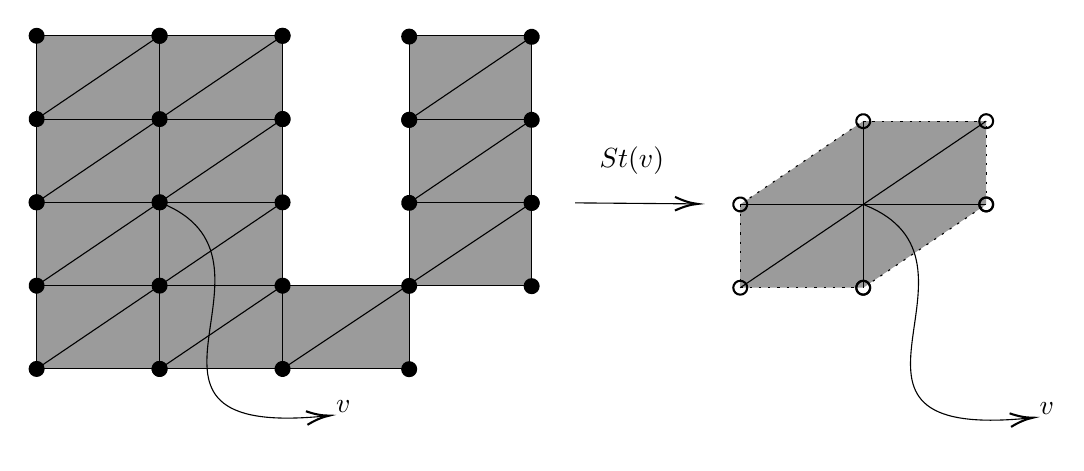
\begin{tikzpicture}[x=0.75pt,y=0.75pt,yscale=-1,xscale=1]
        %uncomment if require: \path (0,433); %set diagram left start at 0, and has height of 433

        %Shape: Rectangle [id:dp6828292052273273] 
        \draw  [fill={rgb, 255:red, 155; green, 155; blue, 155 }  ,fill opacity=1 ] (190.5,10) -- (249.5,10) -- (249.5,130.5) -- (190.5,130.5) -- cycle ;
        %Shape: Rectangle [id:dp1603709832259137] 
        \draw  [fill={rgb, 255:red, 155; green, 155; blue, 155 }  ,fill opacity=1 ] (190.5,50.25) -- (249.5,50.25) -- (249.5,90.25) -- (190.5,90.25) -- cycle ;
        %Shape: Rectangle [id:dp7801372435241032] 
        \draw  [fill={rgb, 255:red, 155; green, 155; blue, 155 }  ,fill opacity=1 ] (129.5,130.5) -- (190.5,130.5) -- (190.5,170.5) -- (129.5,170.5) -- cycle ;
        %Shape: Polygon [id:ds720216123234598] 
        \draw  [draw opacity=0][fill={rgb, 255:red, 155; green, 155; blue, 155 }  ,fill opacity=1 ] (468.5,51.13) -- (468.5,91.25) -- (409.25,131.38) -- (350,131.38) -- (350,91.25) -- (409.25,51.13) -- cycle ;
        %Shape: Rectangle [id:dp29792580873182595] 
        \draw  [fill={rgb, 255:red, 155; green, 155; blue, 155 }  ,fill opacity=1 ] (190.5,90.5) -- (249.5,90.5) -- (249.5,130.5) -- (190.5,130.5) -- cycle ;
        %Shape: Rectangle [id:dp6639087811481719] 
        \draw  [fill={rgb, 255:red, 155; green, 155; blue, 155 }  ,fill opacity=1 ] (11,10) -- (129.5,10) -- (129.5,170.5) -- (11,170.5) -- cycle ;
        %Straight Lines [id:da6575867828932402] 
        \draw    (11,10) -- (11,170.5) ;
        %Straight Lines [id:da8065281350659392] 
        \draw    (11,10) -- (129.5,10) ;
        \draw [shift={(129.5,10)}, rotate = 0] [color={rgb, 255:red, 0; green, 0; blue, 0 }  ][fill={rgb, 255:red, 0; green, 0; blue, 0 }  ][line width=0.75]      (0, 0) circle [x radius= 3.35, y radius= 3.35]   ;
        \draw [shift={(11,10)}, rotate = 0] [color={rgb, 255:red, 0; green, 0; blue, 0 }  ][fill={rgb, 255:red, 0; green, 0; blue, 0 }  ][line width=0.75]      (0, 0) circle [x radius= 3.35, y radius= 3.35]   ;
        %Straight Lines [id:da3992609650184433] 
        \draw    (129.5,10) -- (129.5,170.5) ;
        %Straight Lines [id:da13475589884345496] 
        \draw    (11,170.5) -- (129.5,170.5) ;
        %Straight Lines [id:da4416095201662438] 
        \draw    (70.25,10) -- (70.25,170.5) ;
        \draw [shift={(70.25,170.5)}, rotate = 90] [color={rgb, 255:red, 0; green, 0; blue, 0 }  ][fill={rgb, 255:red, 0; green, 0; blue, 0 }  ][line width=0.75]      (0, 0) circle [x radius= 3.35, y radius= 3.35]   ;
        \draw [shift={(70.25,10)}, rotate = 90] [color={rgb, 255:red, 0; green, 0; blue, 0 }  ][fill={rgb, 255:red, 0; green, 0; blue, 0 }  ][line width=0.75]      (0, 0) circle [x radius= 3.35, y radius= 3.35]   ;
        %Straight Lines [id:da6740170575639275] 
        \draw    (11,90.25) -- (129.5,90.25) ;
        %Straight Lines [id:da719865308555645] 
        \draw    (129.5,10) -- (129.5,90.25) ;
        \draw [shift={(129.5,90.25)}, rotate = 90] [color={rgb, 255:red, 0; green, 0; blue, 0 }  ][fill={rgb, 255:red, 0; green, 0; blue, 0 }  ][line width=0.75]      (0, 0) circle [x radius= 3.35, y radius= 3.35]   ;
        \draw [shift={(129.5,10)}, rotate = 90] [color={rgb, 255:red, 0; green, 0; blue, 0 }  ][fill={rgb, 255:red, 0; green, 0; blue, 0 }  ][line width=0.75]      (0, 0) circle [x radius= 3.35, y radius= 3.35]   ;
        %Straight Lines [id:da7675296220139092] 
        \draw    (11,10) -- (11,90.25) ;
        %Straight Lines [id:da6604115448480403] 
        \draw    (129.5,90.25) -- (129.5,170.5) ;
        %Straight Lines [id:da921763560201903] 
        \draw    (11,90.25) -- (11,170.5) ;
        \draw [shift={(11,170.5)}, rotate = 90] [color={rgb, 255:red, 0; green, 0; blue, 0 }  ][fill={rgb, 255:red, 0; green, 0; blue, 0 }  ][line width=0.75]      (0, 0) circle [x radius= 3.35, y radius= 3.35]   ;
        \draw [shift={(11,90.25)}, rotate = 90] [color={rgb, 255:red, 0; green, 0; blue, 0 }  ][fill={rgb, 255:red, 0; green, 0; blue, 0 }  ][line width=0.75]      (0, 0) circle [x radius= 3.35, y radius= 3.35]   ;
        %Straight Lines [id:da8649318988296271] 
        \draw    (11,130.38) -- (129.5,130.38) ;
        %Straight Lines [id:da16660765957405133] 
        \draw    (11,50.13) -- (129.5,50.13) ;
        \draw [shift={(129.5,50.13)}, rotate = 0] [color={rgb, 255:red, 0; green, 0; blue, 0 }  ][fill={rgb, 255:red, 0; green, 0; blue, 0 }  ][line width=0.75]      (0, 0) circle [x radius= 3.35, y radius= 3.35]   ;
        %Straight Lines [id:da21493603049157772] 
        \draw    (70.25,10) -- (11,50.13) ;
        \draw [shift={(11,50.13)}, rotate = 145.89] [color={rgb, 255:red, 0; green, 0; blue, 0 }  ][fill={rgb, 255:red, 0; green, 0; blue, 0 }  ][line width=0.75]      (0, 0) circle [x radius= 3.35, y radius= 3.35]   ;
        \draw [shift={(70.25,10)}, rotate = 145.89] [color={rgb, 255:red, 0; green, 0; blue, 0 }  ][fill={rgb, 255:red, 0; green, 0; blue, 0 }  ][line width=0.75]      (0, 0) circle [x radius= 3.35, y radius= 3.35]   ;
        %Straight Lines [id:da018520940840161426] 
        \draw    (129.5,10) -- (11,90.25) ;
        \draw [shift={(11,90.25)}, rotate = 145.89] [color={rgb, 255:red, 0; green, 0; blue, 0 }  ][fill={rgb, 255:red, 0; green, 0; blue, 0 }  ][line width=0.75]      (0, 0) circle [x radius= 3.35, y radius= 3.35]   ;
        %Straight Lines [id:da8908508321424791] 
        \draw    (129.5,50.13) -- (11,130.38) ;
        \draw [shift={(11,130.38)}, rotate = 145.89] [color={rgb, 255:red, 0; green, 0; blue, 0 }  ][fill={rgb, 255:red, 0; green, 0; blue, 0 }  ][line width=0.75]      (0, 0) circle [x radius= 3.35, y radius= 3.35]   ;
        \draw [shift={(129.5,50.13)}, rotate = 145.89] [color={rgb, 255:red, 0; green, 0; blue, 0 }  ][fill={rgb, 255:red, 0; green, 0; blue, 0 }  ][line width=0.75]      (0, 0) circle [x radius= 3.35, y radius= 3.35]   ;
        %Straight Lines [id:da10224452058981259] 
        \draw    (129.5,90.25) -- (11,170.5) ;
        %Straight Lines [id:da8535884033018606] 
        \draw    (129.5,130.38) -- (70.25,170.5) ;
        \draw [shift={(70.25,170.5)}, rotate = 145.89] [color={rgb, 255:red, 0; green, 0; blue, 0 }  ][fill={rgb, 255:red, 0; green, 0; blue, 0 }  ][line width=0.75]      (0, 0) circle [x radius= 3.35, y radius= 3.35]   ;
        \draw [shift={(129.5,130.38)}, rotate = 145.89] [color={rgb, 255:red, 0; green, 0; blue, 0 }  ][fill={rgb, 255:red, 0; green, 0; blue, 0 }  ][line width=0.75]      (0, 0) circle [x radius= 3.35, y radius= 3.35]   ;
        %Straight Lines [id:da713065441573842] 
        \draw    (249.5,90.5) -- (129.5,170.5) ;
        \draw [shift={(129.5,170.5)}, rotate = 146.31] [color={rgb, 255:red, 0; green, 0; blue, 0 }  ][fill={rgb, 255:red, 0; green, 0; blue, 0 }  ][line width=0.75]      (0, 0) circle [x radius= 3.35, y radius= 3.35]   ;
        \draw [shift={(249.5,90.5)}, rotate = 146.31] [color={rgb, 255:red, 0; green, 0; blue, 0 }  ][fill={rgb, 255:red, 0; green, 0; blue, 0 }  ][line width=0.75]      (0, 0) circle [x radius= 3.35, y radius= 3.35]   ;
        %Straight Lines [id:da4858360870120242] 
        \draw    (190.5,90.5) -- (249.5,50.5) ;
        \draw [shift={(249.5,50.5)}, rotate = 325.86] [color={rgb, 255:red, 0; green, 0; blue, 0 }  ][fill={rgb, 255:red, 0; green, 0; blue, 0 }  ][line width=0.75]      (0, 0) circle [x radius= 3.35, y radius= 3.35]   ;
        \draw [shift={(190.5,90.5)}, rotate = 325.86] [color={rgb, 255:red, 0; green, 0; blue, 0 }  ][fill={rgb, 255:red, 0; green, 0; blue, 0 }  ][line width=0.75]      (0, 0) circle [x radius= 3.35, y radius= 3.35]   ;
        %Straight Lines [id:da10590665049175874] 
        \draw    (190.5,50.5) -- (249.5,10.5) ;
        \draw [shift={(249.5,10.5)}, rotate = 325.86] [color={rgb, 255:red, 0; green, 0; blue, 0 }  ][fill={rgb, 255:red, 0; green, 0; blue, 0 }  ][line width=0.75]      (0, 0) circle [x radius= 3.35, y radius= 3.35]   ;
        \draw [shift={(190.5,50.5)}, rotate = 325.86] [color={rgb, 255:red, 0; green, 0; blue, 0 }  ][fill={rgb, 255:red, 0; green, 0; blue, 0 }  ][line width=0.75]      (0, 0) circle [x radius= 3.35, y radius= 3.35]   ;
        %Curve Lines [id:da3048204937708163] 
        \draw    (70.25,90.25) .. controls (140.15,117.36) and (36.55,204.62) .. (150.27,193.18) ;
        \draw [shift={(152,193)}, rotate = 173.88] [color={rgb, 255:red, 0; green, 0; blue, 0 }  ][line width=0.75]    (10.93,-3.29) .. controls (6.95,-1.4) and (3.31,-0.3) .. (0,0) .. controls (3.31,0.3) and (6.95,1.4) .. (10.93,3.29)   ;
        %Straight Lines [id:da47235478955329335] 
        \draw    (350,91.25) -- (468.5,91.25) ;
        %Straight Lines [id:da2835426229932716] 
        \draw    (468.5,51.13) -- (350,131.38) ;
        %Curve Lines [id:da035665221490229326] 
        \draw    (409.25,91.25) .. controls (479.15,118.36) and (375.55,205.62) .. (489.27,194.18) ;
        \draw [shift={(491,194)}, rotate = 173.88] [color={rgb, 255:red, 0; green, 0; blue, 0 }  ][line width=0.75]    (10.93,-3.29) .. controls (6.95,-1.4) and (3.31,-0.3) .. (0,0) .. controls (3.31,0.3) and (6.95,1.4) .. (10.93,3.29)   ;
        %Straight Lines [id:da7015390425861685] 
        \draw    (270.5,90.5) -- (327.5,90.98) ;
        \draw [shift={(329.5,91)}, rotate = 180.49] [color={rgb, 255:red, 0; green, 0; blue, 0 }  ][line width=0.75]    (10.93,-3.29) .. controls (6.95,-1.4) and (3.31,-0.3) .. (0,0) .. controls (3.31,0.3) and (6.95,1.4) .. (10.93,3.29)   ;
        %Straight Lines [id:da430224578320642] 
        \draw  [dash pattern={on 0.84pt off 2.51pt}]  (468.5,53.48) -- (468.5,88.9) ;
        \draw [shift={(468.5,91.25)}, rotate = 90] [color={rgb, 255:red, 0; green, 0; blue, 0 }  ][line width=0.75]      (0, 0) circle [x radius= 3.35, y radius= 3.35]   ;
        \draw [shift={(468.5,51.13)}, rotate = 90] [color={rgb, 255:red, 0; green, 0; blue, 0 }  ][line width=0.75]      (0, 0) circle [x radius= 3.35, y radius= 3.35]   ;
        %Straight Lines [id:da37030714095060646] 
        \draw  [dash pattern={on 0.84pt off 2.51pt}]  (466.55,92.57) -- (411.2,130.06) ;
        \draw [shift={(409.25,131.38)}, rotate = 145.89] [color={rgb, 255:red, 0; green, 0; blue, 0 }  ][line width=0.75]      (0, 0) circle [x radius= 3.35, y radius= 3.35]   ;
        \draw [shift={(468.5,91.25)}, rotate = 145.89] [color={rgb, 255:red, 0; green, 0; blue, 0 }  ][line width=0.75]      (0, 0) circle [x radius= 3.35, y radius= 3.35]   ;
        %Straight Lines [id:da5836144013688405] 
        \draw  [dash pattern={on 0.84pt off 2.51pt}]  (350,131.38) -- (406.9,131.38) ;
        \draw [shift={(409.25,131.38)}, rotate = 0] [color={rgb, 255:red, 0; green, 0; blue, 0 }  ][line width=0.75]      (0, 0) circle [x radius= 3.35, y radius= 3.35]   ;
        %Straight Lines [id:da40369009096787956] 
        \draw    (409.25,131.38) -- (409.25,51.13) ;
        %Straight Lines [id:da8020528470081729] 
        \draw  [dash pattern={on 0.84pt off 2.51pt}]  (407.3,52.44) -- (351.95,89.93) ;
        \draw [shift={(350,91.25)}, rotate = 145.89] [color={rgb, 255:red, 0; green, 0; blue, 0 }  ][line width=0.75]      (0, 0) circle [x radius= 3.35, y radius= 3.35]   ;
        \draw [shift={(409.25,51.13)}, rotate = 145.89] [color={rgb, 255:red, 0; green, 0; blue, 0 }  ][line width=0.75]      (0, 0) circle [x radius= 3.35, y radius= 3.35]   ;
        %Straight Lines [id:da7950005502913955] 
        \draw  [dash pattern={on 0.84pt off 2.51pt}]  (350,91.25) -- (350,129.03) ;
        \draw [shift={(350,131.38)}, rotate = 90] [color={rgb, 255:red, 0; green, 0; blue, 0 }  ][line width=0.75]      (0, 0) circle [x radius= 3.35, y radius= 3.35]   ;
        %Straight Lines [id:da9734858002385687] 
        \draw  [dash pattern={on 0.84pt off 2.51pt}]  (409.25,51.13) -- (468.5,51.13) ;
        %Straight Lines [id:da7996705859516942] 
        \draw    (70.25,90.25) -- (70.25,130.38) ;
        \draw [shift={(70.25,130.38)}, rotate = 90] [color={rgb, 255:red, 0; green, 0; blue, 0 }  ][fill={rgb, 255:red, 0; green, 0; blue, 0 }  ][line width=0.75]      (0, 0) circle [x radius= 3.35, y radius= 3.35]   ;
        \draw [shift={(70.25,90.25)}, rotate = 90] [color={rgb, 255:red, 0; green, 0; blue, 0 }  ][fill={rgb, 255:red, 0; green, 0; blue, 0 }  ][line width=0.75]      (0, 0) circle [x radius= 3.35, y radius= 3.35]   ;
        %Straight Lines [id:da3138524723474039] 
        \draw    (70.25,50.13) -- (70.25,90.25) ;
        \draw [shift={(70.25,90.25)}, rotate = 90] [color={rgb, 255:red, 0; green, 0; blue, 0 }  ][fill={rgb, 255:red, 0; green, 0; blue, 0 }  ][line width=0.75]      (0, 0) circle [x radius= 3.35, y radius= 3.35]   ;
        \draw [shift={(70.25,50.13)}, rotate = 90] [color={rgb, 255:red, 0; green, 0; blue, 0 }  ][fill={rgb, 255:red, 0; green, 0; blue, 0 }  ][line width=0.75]      (0, 0) circle [x radius= 3.35, y radius= 3.35]   ;
        %Straight Lines [id:da6901146317341891] 
        \draw    (190.5,130.5) -- (190.5,170.63) ;
        \draw [shift={(190.5,170.63)}, rotate = 90] [color={rgb, 255:red, 0; green, 0; blue, 0 }  ][fill={rgb, 255:red, 0; green, 0; blue, 0 }  ][line width=0.75]      (0, 0) circle [x radius= 3.35, y radius= 3.35]   ;
        \draw [shift={(190.5,130.5)}, rotate = 90] [color={rgb, 255:red, 0; green, 0; blue, 0 }  ][fill={rgb, 255:red, 0; green, 0; blue, 0 }  ][line width=0.75]      (0, 0) circle [x radius= 3.35, y radius= 3.35]   ;
        %Straight Lines [id:da5863145317047915] 
        \draw    (190.5,10.38) -- (190.5,50.5) ;
        \draw [shift={(190.5,50.5)}, rotate = 90] [color={rgb, 255:red, 0; green, 0; blue, 0 }  ][fill={rgb, 255:red, 0; green, 0; blue, 0 }  ][line width=0.75]      (0, 0) circle [x radius= 3.35, y radius= 3.35]   ;
        \draw [shift={(190.5,10.38)}, rotate = 90] [color={rgb, 255:red, 0; green, 0; blue, 0 }  ][fill={rgb, 255:red, 0; green, 0; blue, 0 }  ][line width=0.75]      (0, 0) circle [x radius= 3.35, y radius= 3.35]   ;
        %Straight Lines [id:da15956690296671794] 
        \draw    (249.5,90.5) -- (249.5,130.63) ;
        \draw [shift={(249.5,130.63)}, rotate = 90] [color={rgb, 255:red, 0; green, 0; blue, 0 }  ][fill={rgb, 255:red, 0; green, 0; blue, 0 }  ][line width=0.75]      (0, 0) circle [x radius= 3.35, y radius= 3.35]   ;
        \draw [shift={(249.5,90.5)}, rotate = 90] [color={rgb, 255:red, 0; green, 0; blue, 0 }  ][fill={rgb, 255:red, 0; green, 0; blue, 0 }  ][line width=0.75]      (0, 0) circle [x radius= 3.35, y radius= 3.35]   ;

        % Text Node
        \draw (154,184.4) node [anchor=north west][inner sep=0.75pt]    {$v$};
        % Text Node
        \draw (493,185.4) node [anchor=north west][inner sep=0.75pt]    {$v$};
        % Text Node
        \draw (281,62.4) node [anchor=north west][inner sep=0.75pt]    {$St( v)$};


    \end{tikzpicture}

\end{center}
\paragraph{Porprietà} $St(v)$ è un insieme aperto di $|K|$
\begin{proof}
    $|K|\setminus St(v)$ è l'unione di tutti i simplessi di $K$ che non hanno $v$ come vertice.\\
    $|K|\setminus St(v)=|L|$, con $L$ sottocomplesso di $K$, il quale è un chiuso rispetto alla topologia di $|K|$
\end{proof}
\paragraph{Morale} $St(v)$ è il più piccolo intorno aperto di $v$ deducibile dalla struttura combinatoriale di $K$
\begin{definition}[Star chiusa]
    Per ogni vertice $v\in K^{(0)}$, definiamo star chiusa di $v$ la chiusura (nel senso topologico) della star di $v$.\\
    Useremo una delle seguenti notazioni
    \[
        \overline{St}(v)\quad \overline{St(v)}\quad ClSt(v)
    \]
    o per specificare il complesso
    \[
        \overline{St}(v,K)\quad \overline{St(v,K)}\quad ClSt(v,K)
    \]
\end{definition}
\begin{center}


    \tikzset{every picture/.style={line width=0.75pt}} %set default line width to 0.75pt        

    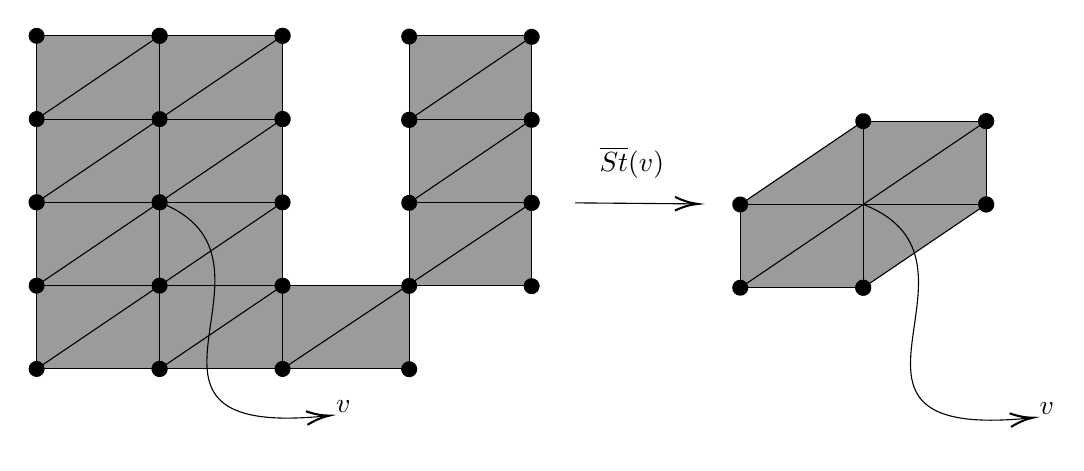
\begin{tikzpicture}[x=0.75pt,y=0.75pt,yscale=-1,xscale=1]
        %uncomment if require: \path (0,433); %set diagram left start at 0, and has height of 433

        %Shape: Rectangle [id:dp6828292052273273] 
        \draw  [fill={rgb, 255:red, 155; green, 155; blue, 155 }  ,fill opacity=1 ] (190.5,10) -- (249.5,10) -- (249.5,130.5) -- (190.5,130.5) -- cycle ;
        %Shape: Rectangle [id:dp1603709832259137] 
        \draw  [fill={rgb, 255:red, 155; green, 155; blue, 155 }  ,fill opacity=1 ] (190.5,50.25) -- (249.5,50.25) -- (249.5,90.25) -- (190.5,90.25) -- cycle ;
        %Shape: Rectangle [id:dp7801372435241032] 
        \draw  [fill={rgb, 255:red, 155; green, 155; blue, 155 }  ,fill opacity=1 ] (129.5,130.5) -- (190.5,130.5) -- (190.5,170.5) -- (129.5,170.5) -- cycle ;
        %Shape: Polygon [id:ds720216123234598] 
        \draw  [draw opacity=0][fill={rgb, 255:red, 155; green, 155; blue, 155 }  ,fill opacity=1 ] (468.5,51.13) -- (468.5,91.25) -- (409.25,131.38) -- (350,131.38) -- (350,91.25) -- (409.25,51.13) -- cycle ;
        %Shape: Rectangle [id:dp29792580873182595] 
        \draw  [fill={rgb, 255:red, 155; green, 155; blue, 155 }  ,fill opacity=1 ] (190.5,90.5) -- (249.5,90.5) -- (249.5,130.5) -- (190.5,130.5) -- cycle ;
        %Shape: Rectangle [id:dp6639087811481719] 
        \draw  [fill={rgb, 255:red, 155; green, 155; blue, 155 }  ,fill opacity=1 ] (11,10) -- (129.5,10) -- (129.5,170.5) -- (11,170.5) -- cycle ;
        %Straight Lines [id:da6575867828932402] 
        \draw    (11,10) -- (11,170.5) ;
        %Straight Lines [id:da8065281350659392] 
        \draw    (11,10) -- (129.5,10) ;
        \draw [shift={(129.5,10)}, rotate = 0] [color={rgb, 255:red, 0; green, 0; blue, 0 }  ][fill={rgb, 255:red, 0; green, 0; blue, 0 }  ][line width=0.75]      (0, 0) circle [x radius= 3.35, y radius= 3.35]   ;
        \draw [shift={(11,10)}, rotate = 0] [color={rgb, 255:red, 0; green, 0; blue, 0 }  ][fill={rgb, 255:red, 0; green, 0; blue, 0 }  ][line width=0.75]      (0, 0) circle [x radius= 3.35, y radius= 3.35]   ;
        %Straight Lines [id:da3992609650184433] 
        \draw    (129.5,10) -- (129.5,170.5) ;
        %Straight Lines [id:da13475589884345496] 
        \draw    (11,170.5) -- (129.5,170.5) ;
        %Straight Lines [id:da4416095201662438] 
        \draw    (70.25,10) -- (70.25,170.5) ;
        \draw [shift={(70.25,170.5)}, rotate = 90] [color={rgb, 255:red, 0; green, 0; blue, 0 }  ][fill={rgb, 255:red, 0; green, 0; blue, 0 }  ][line width=0.75]      (0, 0) circle [x radius= 3.35, y radius= 3.35]   ;
        \draw [shift={(70.25,10)}, rotate = 90] [color={rgb, 255:red, 0; green, 0; blue, 0 }  ][fill={rgb, 255:red, 0; green, 0; blue, 0 }  ][line width=0.75]      (0, 0) circle [x radius= 3.35, y radius= 3.35]   ;
        %Straight Lines [id:da6740170575639275] 
        \draw    (11,90.25) -- (129.5,90.25) ;
        %Straight Lines [id:da719865308555645] 
        \draw    (129.5,10) -- (129.5,90.25) ;
        \draw [shift={(129.5,90.25)}, rotate = 90] [color={rgb, 255:red, 0; green, 0; blue, 0 }  ][fill={rgb, 255:red, 0; green, 0; blue, 0 }  ][line width=0.75]      (0, 0) circle [x radius= 3.35, y radius= 3.35]   ;
        \draw [shift={(129.5,10)}, rotate = 90] [color={rgb, 255:red, 0; green, 0; blue, 0 }  ][fill={rgb, 255:red, 0; green, 0; blue, 0 }  ][line width=0.75]      (0, 0) circle [x radius= 3.35, y radius= 3.35]   ;
        %Straight Lines [id:da7675296220139092] 
        \draw    (11,10) -- (11,90.25) ;
        %Straight Lines [id:da6604115448480403] 
        \draw    (129.5,90.25) -- (129.5,170.5) ;
        %Straight Lines [id:da921763560201903] 
        \draw    (11,90.25) -- (11,170.5) ;
        \draw [shift={(11,170.5)}, rotate = 90] [color={rgb, 255:red, 0; green, 0; blue, 0 }  ][fill={rgb, 255:red, 0; green, 0; blue, 0 }  ][line width=0.75]      (0, 0) circle [x radius= 3.35, y radius= 3.35]   ;
        \draw [shift={(11,90.25)}, rotate = 90] [color={rgb, 255:red, 0; green, 0; blue, 0 }  ][fill={rgb, 255:red, 0; green, 0; blue, 0 }  ][line width=0.75]      (0, 0) circle [x radius= 3.35, y radius= 3.35]   ;
        %Straight Lines [id:da8649318988296271] 
        \draw    (11,130.38) -- (129.5,130.38) ;
        %Straight Lines [id:da16660765957405133] 
        \draw    (11,50.13) -- (129.5,50.13) ;
        \draw [shift={(129.5,50.13)}, rotate = 0] [color={rgb, 255:red, 0; green, 0; blue, 0 }  ][fill={rgb, 255:red, 0; green, 0; blue, 0 }  ][line width=0.75]      (0, 0) circle [x radius= 3.35, y radius= 3.35]   ;
        %Straight Lines [id:da21493603049157772] 
        \draw    (70.25,10) -- (11,50.13) ;
        \draw [shift={(11,50.13)}, rotate = 145.89] [color={rgb, 255:red, 0; green, 0; blue, 0 }  ][fill={rgb, 255:red, 0; green, 0; blue, 0 }  ][line width=0.75]      (0, 0) circle [x radius= 3.35, y radius= 3.35]   ;
        \draw [shift={(70.25,10)}, rotate = 145.89] [color={rgb, 255:red, 0; green, 0; blue, 0 }  ][fill={rgb, 255:red, 0; green, 0; blue, 0 }  ][line width=0.75]      (0, 0) circle [x radius= 3.35, y radius= 3.35]   ;
        %Straight Lines [id:da018520940840161426] 
        \draw    (129.5,10) -- (11,90.25) ;
        \draw [shift={(11,90.25)}, rotate = 145.89] [color={rgb, 255:red, 0; green, 0; blue, 0 }  ][fill={rgb, 255:red, 0; green, 0; blue, 0 }  ][line width=0.75]      (0, 0) circle [x radius= 3.35, y radius= 3.35]   ;
        %Straight Lines [id:da8908508321424791] 
        \draw    (129.5,50.13) -- (11,130.38) ;
        \draw [shift={(11,130.38)}, rotate = 145.89] [color={rgb, 255:red, 0; green, 0; blue, 0 }  ][fill={rgb, 255:red, 0; green, 0; blue, 0 }  ][line width=0.75]      (0, 0) circle [x radius= 3.35, y radius= 3.35]   ;
        \draw [shift={(129.5,50.13)}, rotate = 145.89] [color={rgb, 255:red, 0; green, 0; blue, 0 }  ][fill={rgb, 255:red, 0; green, 0; blue, 0 }  ][line width=0.75]      (0, 0) circle [x radius= 3.35, y radius= 3.35]   ;
        %Straight Lines [id:da10224452058981259] 
        \draw    (129.5,90.25) -- (11,170.5) ;
        %Straight Lines [id:da8535884033018606] 
        \draw    (129.5,130.38) -- (70.25,170.5) ;
        \draw [shift={(70.25,170.5)}, rotate = 145.89] [color={rgb, 255:red, 0; green, 0; blue, 0 }  ][fill={rgb, 255:red, 0; green, 0; blue, 0 }  ][line width=0.75]      (0, 0) circle [x radius= 3.35, y radius= 3.35]   ;
        \draw [shift={(129.5,130.38)}, rotate = 145.89] [color={rgb, 255:red, 0; green, 0; blue, 0 }  ][fill={rgb, 255:red, 0; green, 0; blue, 0 }  ][line width=0.75]      (0, 0) circle [x radius= 3.35, y radius= 3.35]   ;
        %Straight Lines [id:da713065441573842] 
        \draw    (249.5,90.5) -- (129.5,170.5) ;
        \draw [shift={(129.5,170.5)}, rotate = 146.31] [color={rgb, 255:red, 0; green, 0; blue, 0 }  ][fill={rgb, 255:red, 0; green, 0; blue, 0 }  ][line width=0.75]      (0, 0) circle [x radius= 3.35, y radius= 3.35]   ;
        \draw [shift={(249.5,90.5)}, rotate = 146.31] [color={rgb, 255:red, 0; green, 0; blue, 0 }  ][fill={rgb, 255:red, 0; green, 0; blue, 0 }  ][line width=0.75]      (0, 0) circle [x radius= 3.35, y radius= 3.35]   ;
        %Straight Lines [id:da4858360870120242] 
        \draw    (190.5,90.5) -- (249.5,50.5) ;
        \draw [shift={(249.5,50.5)}, rotate = 325.86] [color={rgb, 255:red, 0; green, 0; blue, 0 }  ][fill={rgb, 255:red, 0; green, 0; blue, 0 }  ][line width=0.75]      (0, 0) circle [x radius= 3.35, y radius= 3.35]   ;
        \draw [shift={(190.5,90.5)}, rotate = 325.86] [color={rgb, 255:red, 0; green, 0; blue, 0 }  ][fill={rgb, 255:red, 0; green, 0; blue, 0 }  ][line width=0.75]      (0, 0) circle [x radius= 3.35, y radius= 3.35]   ;
        %Straight Lines [id:da10590665049175874] 
        \draw    (190.5,50.5) -- (249.5,10.5) ;
        \draw [shift={(249.5,10.5)}, rotate = 325.86] [color={rgb, 255:red, 0; green, 0; blue, 0 }  ][fill={rgb, 255:red, 0; green, 0; blue, 0 }  ][line width=0.75]      (0, 0) circle [x radius= 3.35, y radius= 3.35]   ;
        \draw [shift={(190.5,50.5)}, rotate = 325.86] [color={rgb, 255:red, 0; green, 0; blue, 0 }  ][fill={rgb, 255:red, 0; green, 0; blue, 0 }  ][line width=0.75]      (0, 0) circle [x radius= 3.35, y radius= 3.35]   ;
        %Curve Lines [id:da3048204937708163] 
        \draw    (70.25,90.25) .. controls (140.15,117.36) and (36.55,204.62) .. (150.27,193.18) ;
        \draw [shift={(152,193)}, rotate = 173.88] [color={rgb, 255:red, 0; green, 0; blue, 0 }  ][line width=0.75]    (10.93,-3.29) .. controls (6.95,-1.4) and (3.31,-0.3) .. (0,0) .. controls (3.31,0.3) and (6.95,1.4) .. (10.93,3.29)   ;
        %Straight Lines [id:da47235478955329335] 
        \draw    (350,91.25) -- (468.5,91.25) ;
        %Straight Lines [id:da2835426229932716] 
        \draw    (468.5,51.13) -- (350,131.38) ;
        %Curve Lines [id:da035665221490229326] 
        \draw    (409.25,91.25) .. controls (479.15,118.36) and (375.55,205.62) .. (489.27,194.18) ;
        \draw [shift={(491,194)}, rotate = 173.88] [color={rgb, 255:red, 0; green, 0; blue, 0 }  ][line width=0.75]    (10.93,-3.29) .. controls (6.95,-1.4) and (3.31,-0.3) .. (0,0) .. controls (3.31,0.3) and (6.95,1.4) .. (10.93,3.29)   ;
        %Straight Lines [id:da7015390425861685] 
        \draw    (270.5,90.5) -- (327.5,90.98) ;
        \draw [shift={(329.5,91)}, rotate = 180.49] [color={rgb, 255:red, 0; green, 0; blue, 0 }  ][line width=0.75]    (10.93,-3.29) .. controls (6.95,-1.4) and (3.31,-0.3) .. (0,0) .. controls (3.31,0.3) and (6.95,1.4) .. (10.93,3.29)   ;
        %Straight Lines [id:da430224578320642] 
        \draw    (468.5,53.48) -- (468.5,91.25) ;
        \draw [shift={(468.5,91.25)}, rotate = 90] [color={rgb, 255:red, 0; green, 0; blue, 0 }  ][fill={rgb, 255:red, 0; green, 0; blue, 0 }  ][line width=0.75]      (0, 0) circle [x radius= 3.35, y radius= 3.35]   ;
        \draw [shift={(468.5,51.13)}, rotate = 90] [color={rgb, 255:red, 0; green, 0; blue, 0 }  ][line width=0.75]      (0, 0) circle [x radius= 3.35, y radius= 3.35]   ;
        %Straight Lines [id:da37030714095060646] 
        \draw    (466.55,92.57) -- (409.25,131.38) ;
        \draw [shift={(409.25,131.38)}, rotate = 145.89] [color={rgb, 255:red, 0; green, 0; blue, 0 }  ][fill={rgb, 255:red, 0; green, 0; blue, 0 }  ][line width=0.75]      (0, 0) circle [x radius= 3.35, y radius= 3.35]   ;
        \draw [shift={(468.5,91.25)}, rotate = 145.89] [color={rgb, 255:red, 0; green, 0; blue, 0 }  ][line width=0.75]      (0, 0) circle [x radius= 3.35, y radius= 3.35]   ;
        %Straight Lines [id:da5836144013688405] 
        \draw    (350,131.38) -- (406.9,131.38) ;
        \draw [shift={(409.25,131.38)}, rotate = 0] [color={rgb, 255:red, 0; green, 0; blue, 0 }  ][line width=0.75]      (0, 0) circle [x radius= 3.35, y radius= 3.35]   ;
        %Straight Lines [id:da40369009096787956] 
        \draw    (409.25,131.38) -- (409.25,51.13) ;
        %Straight Lines [id:da8020528470081729] 
        \draw    (409.25,51.13) -- (350,91.25) ;
        \draw [shift={(350,91.25)}, rotate = 145.89] [color={rgb, 255:red, 0; green, 0; blue, 0 }  ][fill={rgb, 255:red, 0; green, 0; blue, 0 }  ][line width=0.75]      (0, 0) circle [x radius= 3.35, y radius= 3.35]   ;
        \draw [shift={(409.25,51.13)}, rotate = 145.89] [color={rgb, 255:red, 0; green, 0; blue, 0 }  ][fill={rgb, 255:red, 0; green, 0; blue, 0 }  ][line width=0.75]      (0, 0) circle [x radius= 3.35, y radius= 3.35]   ;
        %Straight Lines [id:da7950005502913955] 
        \draw    (350,91.25) -- (350,131.38) ;
        \draw [shift={(350,131.38)}, rotate = 90] [color={rgb, 255:red, 0; green, 0; blue, 0 }  ][fill={rgb, 255:red, 0; green, 0; blue, 0 }  ][line width=0.75]      (0, 0) circle [x radius= 3.35, y radius= 3.35]   ;
        %Straight Lines [id:da9734858002385687] 
        \draw    (409.25,51.13) -- (468.5,51.13) ;
        \draw [shift={(468.5,51.13)}, rotate = 0] [color={rgb, 255:red, 0; green, 0; blue, 0 }  ][fill={rgb, 255:red, 0; green, 0; blue, 0 }  ][line width=0.75]      (0, 0) circle [x radius= 3.35, y radius= 3.35]   ;
        %Straight Lines [id:da7996705859516942] 
        \draw    (70.25,90.25) -- (70.25,130.38) ;
        \draw [shift={(70.25,130.38)}, rotate = 90] [color={rgb, 255:red, 0; green, 0; blue, 0 }  ][fill={rgb, 255:red, 0; green, 0; blue, 0 }  ][line width=0.75]      (0, 0) circle [x radius= 3.35, y radius= 3.35]   ;
        \draw [shift={(70.25,90.25)}, rotate = 90] [color={rgb, 255:red, 0; green, 0; blue, 0 }  ][fill={rgb, 255:red, 0; green, 0; blue, 0 }  ][line width=0.75]      (0, 0) circle [x radius= 3.35, y radius= 3.35]   ;
        %Straight Lines [id:da3138524723474039] 
        \draw    (70.25,50.13) -- (70.25,90.25) ;
        \draw [shift={(70.25,90.25)}, rotate = 90] [color={rgb, 255:red, 0; green, 0; blue, 0 }  ][fill={rgb, 255:red, 0; green, 0; blue, 0 }  ][line width=0.75]      (0, 0) circle [x radius= 3.35, y radius= 3.35]   ;
        \draw [shift={(70.25,50.13)}, rotate = 90] [color={rgb, 255:red, 0; green, 0; blue, 0 }  ][fill={rgb, 255:red, 0; green, 0; blue, 0 }  ][line width=0.75]      (0, 0) circle [x radius= 3.35, y radius= 3.35]   ;
        %Straight Lines [id:da6901146317341891] 
        \draw    (190.5,130.5) -- (190.5,170.63) ;
        \draw [shift={(190.5,170.63)}, rotate = 90] [color={rgb, 255:red, 0; green, 0; blue, 0 }  ][fill={rgb, 255:red, 0; green, 0; blue, 0 }  ][line width=0.75]      (0, 0) circle [x radius= 3.35, y radius= 3.35]   ;
        \draw [shift={(190.5,130.5)}, rotate = 90] [color={rgb, 255:red, 0; green, 0; blue, 0 }  ][fill={rgb, 255:red, 0; green, 0; blue, 0 }  ][line width=0.75]      (0, 0) circle [x radius= 3.35, y radius= 3.35]   ;
        %Straight Lines [id:da5863145317047915] 
        \draw    (190.5,10.38) -- (190.5,50.5) ;
        \draw [shift={(190.5,50.5)}, rotate = 90] [color={rgb, 255:red, 0; green, 0; blue, 0 }  ][fill={rgb, 255:red, 0; green, 0; blue, 0 }  ][line width=0.75]      (0, 0) circle [x radius= 3.35, y radius= 3.35]   ;
        \draw [shift={(190.5,10.38)}, rotate = 90] [color={rgb, 255:red, 0; green, 0; blue, 0 }  ][fill={rgb, 255:red, 0; green, 0; blue, 0 }  ][line width=0.75]      (0, 0) circle [x radius= 3.35, y radius= 3.35]   ;
        %Straight Lines [id:da15956690296671794] 
        \draw    (249.5,90.5) -- (249.5,130.63) ;
        \draw [shift={(249.5,130.63)}, rotate = 90] [color={rgb, 255:red, 0; green, 0; blue, 0 }  ][fill={rgb, 255:red, 0; green, 0; blue, 0 }  ][line width=0.75]      (0, 0) circle [x radius= 3.35, y radius= 3.35]   ;
        \draw [shift={(249.5,90.5)}, rotate = 90] [color={rgb, 255:red, 0; green, 0; blue, 0 }  ][fill={rgb, 255:red, 0; green, 0; blue, 0 }  ][line width=0.75]      (0, 0) circle [x radius= 3.35, y radius= 3.35]   ;

        % Text Node
        \draw (154,184.4) node [anchor=north west][inner sep=0.75pt]    {$v$};
        % Text Node
        \draw (493,185.4) node [anchor=north west][inner sep=0.75pt]    {$v$};
        % Text Node
        \draw (281,62.4) node [anchor=north west][inner sep=0.75pt]    {$\overline{St}( v)$};


    \end{tikzpicture}

\end{center}
\paragraph{Proprietà}
\begin{itemize}
    \item \cstar{v} è un insieme chiuso di $|K|$ (con la topologia di $|K$)
    \item \cstar{v} è lo spazio soggiacente del sottocomplesso $L'\subseteq K$ formato da tutti i cimplessi con $v$ come vertice
\end{itemize}
\begin{definition}[Link]
    Per ogni vertice $v\in K^{(0)}$, definiamo link di $v$ la differenza tra
    \[
        Lk:=\cstar{v}\setminus St(v)
    \]
\end{definition}
\begin{center}


    \tikzset{every picture/.style={line width=0.75pt}} %set default line width to 0.75pt        

    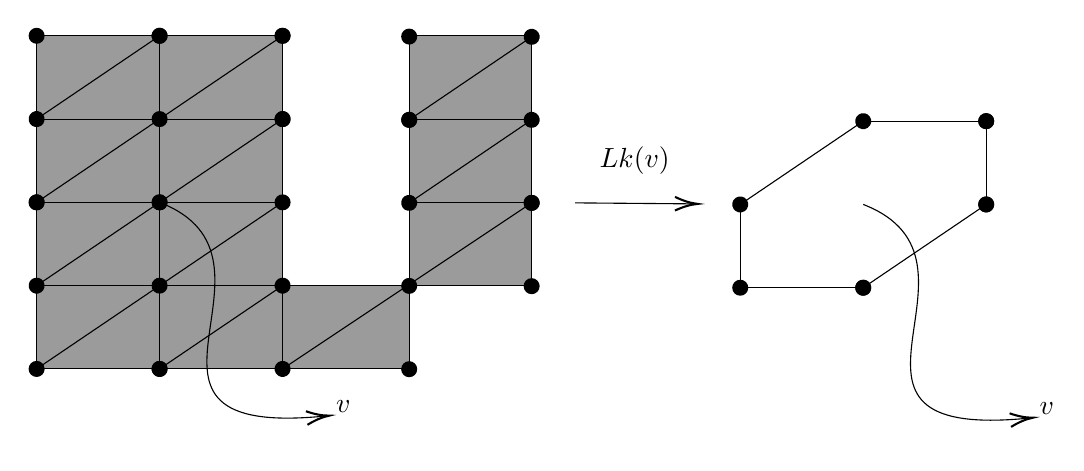
\begin{tikzpicture}[x=0.75pt,y=0.75pt,yscale=-1,xscale=1]
        %uncomment if require: \path (0,433); %set diagram left start at 0, and has height of 433

        %Shape: Rectangle [id:dp6828292052273273] 
        \draw  [fill={rgb, 255:red, 155; green, 155; blue, 155 }  ,fill opacity=1 ] (190.5,10) -- (249.5,10) -- (249.5,130.5) -- (190.5,130.5) -- cycle ;
        %Shape: Rectangle [id:dp1603709832259137] 
        \draw  [fill={rgb, 255:red, 155; green, 155; blue, 155 }  ,fill opacity=1 ] (190.5,50.25) -- (249.5,50.25) -- (249.5,90.25) -- (190.5,90.25) -- cycle ;
        %Shape: Rectangle [id:dp7801372435241032] 
        \draw  [fill={rgb, 255:red, 155; green, 155; blue, 155 }  ,fill opacity=1 ] (129.5,130.5) -- (190.5,130.5) -- (190.5,170.5) -- (129.5,170.5) -- cycle ;
        %Shape: Rectangle [id:dp29792580873182595] 
        \draw  [fill={rgb, 255:red, 155; green, 155; blue, 155 }  ,fill opacity=1 ] (190.5,90.5) -- (249.5,90.5) -- (249.5,130.5) -- (190.5,130.5) -- cycle ;
        %Shape: Rectangle [id:dp6639087811481719] 
        \draw  [fill={rgb, 255:red, 155; green, 155; blue, 155 }  ,fill opacity=1 ] (11,10) -- (129.5,10) -- (129.5,170.5) -- (11,170.5) -- cycle ;
        %Straight Lines [id:da6575867828932402] 
        \draw    (11,10) -- (11,170.5) ;
        %Straight Lines [id:da8065281350659392] 
        \draw    (11,10) -- (129.5,10) ;
        \draw [shift={(129.5,10)}, rotate = 0] [color={rgb, 255:red, 0; green, 0; blue, 0 }  ][fill={rgb, 255:red, 0; green, 0; blue, 0 }  ][line width=0.75]      (0, 0) circle [x radius= 3.35, y radius= 3.35]   ;
        \draw [shift={(11,10)}, rotate = 0] [color={rgb, 255:red, 0; green, 0; blue, 0 }  ][fill={rgb, 255:red, 0; green, 0; blue, 0 }  ][line width=0.75]      (0, 0) circle [x radius= 3.35, y radius= 3.35]   ;
        %Straight Lines [id:da3992609650184433] 
        \draw    (129.5,10) -- (129.5,170.5) ;
        %Straight Lines [id:da13475589884345496] 
        \draw    (11,170.5) -- (129.5,170.5) ;
        %Straight Lines [id:da4416095201662438] 
        \draw    (70.25,10) -- (70.25,170.5) ;
        \draw [shift={(70.25,170.5)}, rotate = 90] [color={rgb, 255:red, 0; green, 0; blue, 0 }  ][fill={rgb, 255:red, 0; green, 0; blue, 0 }  ][line width=0.75]      (0, 0) circle [x radius= 3.35, y radius= 3.35]   ;
        \draw [shift={(70.25,10)}, rotate = 90] [color={rgb, 255:red, 0; green, 0; blue, 0 }  ][fill={rgb, 255:red, 0; green, 0; blue, 0 }  ][line width=0.75]      (0, 0) circle [x radius= 3.35, y radius= 3.35]   ;
        %Straight Lines [id:da6740170575639275] 
        \draw    (11,90.25) -- (129.5,90.25) ;
        %Straight Lines [id:da719865308555645] 
        \draw    (129.5,10) -- (129.5,90.25) ;
        \draw [shift={(129.5,90.25)}, rotate = 90] [color={rgb, 255:red, 0; green, 0; blue, 0 }  ][fill={rgb, 255:red, 0; green, 0; blue, 0 }  ][line width=0.75]      (0, 0) circle [x radius= 3.35, y radius= 3.35]   ;
        \draw [shift={(129.5,10)}, rotate = 90] [color={rgb, 255:red, 0; green, 0; blue, 0 }  ][fill={rgb, 255:red, 0; green, 0; blue, 0 }  ][line width=0.75]      (0, 0) circle [x radius= 3.35, y radius= 3.35]   ;
        %Straight Lines [id:da7675296220139092] 
        \draw    (11,10) -- (11,90.25) ;
        %Straight Lines [id:da6604115448480403] 
        \draw    (129.5,90.25) -- (129.5,170.5) ;
        %Straight Lines [id:da921763560201903] 
        \draw    (11,90.25) -- (11,170.5) ;
        \draw [shift={(11,170.5)}, rotate = 90] [color={rgb, 255:red, 0; green, 0; blue, 0 }  ][fill={rgb, 255:red, 0; green, 0; blue, 0 }  ][line width=0.75]      (0, 0) circle [x radius= 3.35, y radius= 3.35]   ;
        \draw [shift={(11,90.25)}, rotate = 90] [color={rgb, 255:red, 0; green, 0; blue, 0 }  ][fill={rgb, 255:red, 0; green, 0; blue, 0 }  ][line width=0.75]      (0, 0) circle [x radius= 3.35, y radius= 3.35]   ;
        %Straight Lines [id:da8649318988296271] 
        \draw    (11,130.38) -- (129.5,130.38) ;
        %Straight Lines [id:da16660765957405133] 
        \draw    (11,50.13) -- (129.5,50.13) ;
        \draw [shift={(129.5,50.13)}, rotate = 0] [color={rgb, 255:red, 0; green, 0; blue, 0 }  ][fill={rgb, 255:red, 0; green, 0; blue, 0 }  ][line width=0.75]      (0, 0) circle [x radius= 3.35, y radius= 3.35]   ;
        %Straight Lines [id:da21493603049157772] 
        \draw    (70.25,10) -- (11,50.13) ;
        \draw [shift={(11,50.13)}, rotate = 145.89] [color={rgb, 255:red, 0; green, 0; blue, 0 }  ][fill={rgb, 255:red, 0; green, 0; blue, 0 }  ][line width=0.75]      (0, 0) circle [x radius= 3.35, y radius= 3.35]   ;
        \draw [shift={(70.25,10)}, rotate = 145.89] [color={rgb, 255:red, 0; green, 0; blue, 0 }  ][fill={rgb, 255:red, 0; green, 0; blue, 0 }  ][line width=0.75]      (0, 0) circle [x radius= 3.35, y radius= 3.35]   ;
        %Straight Lines [id:da018520940840161426] 
        \draw    (129.5,10) -- (11,90.25) ;
        \draw [shift={(11,90.25)}, rotate = 145.89] [color={rgb, 255:red, 0; green, 0; blue, 0 }  ][fill={rgb, 255:red, 0; green, 0; blue, 0 }  ][line width=0.75]      (0, 0) circle [x radius= 3.35, y radius= 3.35]   ;
        %Straight Lines [id:da8908508321424791] 
        \draw    (129.5,50.13) -- (11,130.38) ;
        \draw [shift={(11,130.38)}, rotate = 145.89] [color={rgb, 255:red, 0; green, 0; blue, 0 }  ][fill={rgb, 255:red, 0; green, 0; blue, 0 }  ][line width=0.75]      (0, 0) circle [x radius= 3.35, y radius= 3.35]   ;
        \draw [shift={(129.5,50.13)}, rotate = 145.89] [color={rgb, 255:red, 0; green, 0; blue, 0 }  ][fill={rgb, 255:red, 0; green, 0; blue, 0 }  ][line width=0.75]      (0, 0) circle [x radius= 3.35, y radius= 3.35]   ;
        %Straight Lines [id:da10224452058981259] 
        \draw    (129.5,90.25) -- (11,170.5) ;
        %Straight Lines [id:da8535884033018606] 
        \draw    (129.5,130.38) -- (70.25,170.5) ;
        \draw [shift={(70.25,170.5)}, rotate = 145.89] [color={rgb, 255:red, 0; green, 0; blue, 0 }  ][fill={rgb, 255:red, 0; green, 0; blue, 0 }  ][line width=0.75]      (0, 0) circle [x radius= 3.35, y radius= 3.35]   ;
        \draw [shift={(129.5,130.38)}, rotate = 145.89] [color={rgb, 255:red, 0; green, 0; blue, 0 }  ][fill={rgb, 255:red, 0; green, 0; blue, 0 }  ][line width=0.75]      (0, 0) circle [x radius= 3.35, y radius= 3.35]   ;
        %Straight Lines [id:da713065441573842] 
        \draw    (249.5,90.5) -- (129.5,170.5) ;
        \draw [shift={(129.5,170.5)}, rotate = 146.31] [color={rgb, 255:red, 0; green, 0; blue, 0 }  ][fill={rgb, 255:red, 0; green, 0; blue, 0 }  ][line width=0.75]      (0, 0) circle [x radius= 3.35, y radius= 3.35]   ;
        \draw [shift={(249.5,90.5)}, rotate = 146.31] [color={rgb, 255:red, 0; green, 0; blue, 0 }  ][fill={rgb, 255:red, 0; green, 0; blue, 0 }  ][line width=0.75]      (0, 0) circle [x radius= 3.35, y radius= 3.35]   ;
        %Straight Lines [id:da4858360870120242] 
        \draw    (190.5,90.5) -- (249.5,50.5) ;
        \draw [shift={(249.5,50.5)}, rotate = 325.86] [color={rgb, 255:red, 0; green, 0; blue, 0 }  ][fill={rgb, 255:red, 0; green, 0; blue, 0 }  ][line width=0.75]      (0, 0) circle [x radius= 3.35, y radius= 3.35]   ;
        \draw [shift={(190.5,90.5)}, rotate = 325.86] [color={rgb, 255:red, 0; green, 0; blue, 0 }  ][fill={rgb, 255:red, 0; green, 0; blue, 0 }  ][line width=0.75]      (0, 0) circle [x radius= 3.35, y radius= 3.35]   ;
        %Straight Lines [id:da10590665049175874] 
        \draw    (190.5,50.5) -- (249.5,10.5) ;
        \draw [shift={(249.5,10.5)}, rotate = 325.86] [color={rgb, 255:red, 0; green, 0; blue, 0 }  ][fill={rgb, 255:red, 0; green, 0; blue, 0 }  ][line width=0.75]      (0, 0) circle [x radius= 3.35, y radius= 3.35]   ;
        \draw [shift={(190.5,50.5)}, rotate = 325.86] [color={rgb, 255:red, 0; green, 0; blue, 0 }  ][fill={rgb, 255:red, 0; green, 0; blue, 0 }  ][line width=0.75]      (0, 0) circle [x radius= 3.35, y radius= 3.35]   ;
        %Curve Lines [id:da3048204937708163] 
        \draw    (70.25,90.25) .. controls (140.15,117.36) and (36.55,204.62) .. (150.27,193.18) ;
        \draw [shift={(152,193)}, rotate = 173.88] [color={rgb, 255:red, 0; green, 0; blue, 0 }  ][line width=0.75]    (10.93,-3.29) .. controls (6.95,-1.4) and (3.31,-0.3) .. (0,0) .. controls (3.31,0.3) and (6.95,1.4) .. (10.93,3.29)   ;
        %Straight Lines [id:da47235478955329335] 
        \draw    (468.5,91.25) ;
        %Straight Lines [id:da2835426229932716] 
        \draw    (468.5,51.13) ;
        %Curve Lines [id:da035665221490229326] 
        \draw    (409.25,91.25) .. controls (479.15,118.36) and (375.55,205.62) .. (489.27,194.18) ;
        \draw [shift={(491,194)}, rotate = 173.88] [color={rgb, 255:red, 0; green, 0; blue, 0 }  ][line width=0.75]    (10.93,-3.29) .. controls (6.95,-1.4) and (3.31,-0.3) .. (0,0) .. controls (3.31,0.3) and (6.95,1.4) .. (10.93,3.29)   ;
        %Straight Lines [id:da7015390425861685] 
        \draw    (270.5,90.5) -- (327.5,90.98) ;
        \draw [shift={(329.5,91)}, rotate = 180.49] [color={rgb, 255:red, 0; green, 0; blue, 0 }  ][line width=0.75]    (10.93,-3.29) .. controls (6.95,-1.4) and (3.31,-0.3) .. (0,0) .. controls (3.31,0.3) and (6.95,1.4) .. (10.93,3.29)   ;
        %Straight Lines [id:da430224578320642] 
        \draw    (468.5,53.48) -- (468.5,91.25) ;
        \draw [shift={(468.5,91.25)}, rotate = 90] [color={rgb, 255:red, 0; green, 0; blue, 0 }  ][fill={rgb, 255:red, 0; green, 0; blue, 0 }  ][line width=0.75]      (0, 0) circle [x radius= 3.35, y radius= 3.35]   ;
        \draw [shift={(468.5,51.13)}, rotate = 90] [color={rgb, 255:red, 0; green, 0; blue, 0 }  ][line width=0.75]      (0, 0) circle [x radius= 3.35, y radius= 3.35]   ;
        %Straight Lines [id:da37030714095060646] 
        \draw    (466.55,92.57) -- (409.25,131.38) ;
        \draw [shift={(409.25,131.38)}, rotate = 145.89] [color={rgb, 255:red, 0; green, 0; blue, 0 }  ][fill={rgb, 255:red, 0; green, 0; blue, 0 }  ][line width=0.75]      (0, 0) circle [x radius= 3.35, y radius= 3.35]   ;
        \draw [shift={(468.5,91.25)}, rotate = 145.89] [color={rgb, 255:red, 0; green, 0; blue, 0 }  ][line width=0.75]      (0, 0) circle [x radius= 3.35, y radius= 3.35]   ;
        %Straight Lines [id:da5836144013688405] 
        \draw    (350,131.38) -- (406.9,131.38) ;
        \draw [shift={(409.25,131.38)}, rotate = 0] [color={rgb, 255:red, 0; green, 0; blue, 0 }  ][line width=0.75]      (0, 0) circle [x radius= 3.35, y radius= 3.35]   ;
        %Straight Lines [id:da40369009096787956] 
        \draw    (409.25,131.38) ;
        %Straight Lines [id:da8020528470081729] 
        \draw    (409.25,51.13) -- (350,91.25) ;
        \draw [shift={(350,91.25)}, rotate = 145.89] [color={rgb, 255:red, 0; green, 0; blue, 0 }  ][fill={rgb, 255:red, 0; green, 0; blue, 0 }  ][line width=0.75]      (0, 0) circle [x radius= 3.35, y radius= 3.35]   ;
        \draw [shift={(409.25,51.13)}, rotate = 145.89] [color={rgb, 255:red, 0; green, 0; blue, 0 }  ][fill={rgb, 255:red, 0; green, 0; blue, 0 }  ][line width=0.75]      (0, 0) circle [x radius= 3.35, y radius= 3.35]   ;
        %Straight Lines [id:da7950005502913955] 
        \draw    (350,91.25) -- (350,131.38) ;
        \draw [shift={(350,131.38)}, rotate = 90] [color={rgb, 255:red, 0; green, 0; blue, 0 }  ][fill={rgb, 255:red, 0; green, 0; blue, 0 }  ][line width=0.75]      (0, 0) circle [x radius= 3.35, y radius= 3.35]   ;
        %Straight Lines [id:da9734858002385687] 
        \draw    (409.25,51.13) -- (468.5,51.13) ;
        \draw [shift={(468.5,51.13)}, rotate = 0] [color={rgb, 255:red, 0; green, 0; blue, 0 }  ][fill={rgb, 255:red, 0; green, 0; blue, 0 }  ][line width=0.75]      (0, 0) circle [x radius= 3.35, y radius= 3.35]   ;
        %Straight Lines [id:da7996705859516942] 
        \draw    (70.25,90.25) -- (70.25,130.38) ;
        \draw [shift={(70.25,130.38)}, rotate = 90] [color={rgb, 255:red, 0; green, 0; blue, 0 }  ][fill={rgb, 255:red, 0; green, 0; blue, 0 }  ][line width=0.75]      (0, 0) circle [x radius= 3.35, y radius= 3.35]   ;
        \draw [shift={(70.25,90.25)}, rotate = 90] [color={rgb, 255:red, 0; green, 0; blue, 0 }  ][fill={rgb, 255:red, 0; green, 0; blue, 0 }  ][line width=0.75]      (0, 0) circle [x radius= 3.35, y radius= 3.35]   ;
        %Straight Lines [id:da3138524723474039] 
        \draw    (70.25,50.13) -- (70.25,90.25) ;
        \draw [shift={(70.25,90.25)}, rotate = 90] [color={rgb, 255:red, 0; green, 0; blue, 0 }  ][fill={rgb, 255:red, 0; green, 0; blue, 0 }  ][line width=0.75]      (0, 0) circle [x radius= 3.35, y radius= 3.35]   ;
        \draw [shift={(70.25,50.13)}, rotate = 90] [color={rgb, 255:red, 0; green, 0; blue, 0 }  ][fill={rgb, 255:red, 0; green, 0; blue, 0 }  ][line width=0.75]      (0, 0) circle [x radius= 3.35, y radius= 3.35]   ;
        %Straight Lines [id:da6901146317341891] 
        \draw    (190.5,130.5) -- (190.5,170.63) ;
        \draw [shift={(190.5,170.63)}, rotate = 90] [color={rgb, 255:red, 0; green, 0; blue, 0 }  ][fill={rgb, 255:red, 0; green, 0; blue, 0 }  ][line width=0.75]      (0, 0) circle [x radius= 3.35, y radius= 3.35]   ;
        \draw [shift={(190.5,130.5)}, rotate = 90] [color={rgb, 255:red, 0; green, 0; blue, 0 }  ][fill={rgb, 255:red, 0; green, 0; blue, 0 }  ][line width=0.75]      (0, 0) circle [x radius= 3.35, y radius= 3.35]   ;
        %Straight Lines [id:da5863145317047915] 
        \draw    (190.5,10.38) -- (190.5,50.5) ;
        \draw [shift={(190.5,50.5)}, rotate = 90] [color={rgb, 255:red, 0; green, 0; blue, 0 }  ][fill={rgb, 255:red, 0; green, 0; blue, 0 }  ][line width=0.75]      (0, 0) circle [x radius= 3.35, y radius= 3.35]   ;
        \draw [shift={(190.5,10.38)}, rotate = 90] [color={rgb, 255:red, 0; green, 0; blue, 0 }  ][fill={rgb, 255:red, 0; green, 0; blue, 0 }  ][line width=0.75]      (0, 0) circle [x radius= 3.35, y radius= 3.35]   ;
        %Straight Lines [id:da15956690296671794] 
        \draw    (249.5,90.5) -- (249.5,130.63) ;
        \draw [shift={(249.5,130.63)}, rotate = 90] [color={rgb, 255:red, 0; green, 0; blue, 0 }  ][fill={rgb, 255:red, 0; green, 0; blue, 0 }  ][line width=0.75]      (0, 0) circle [x radius= 3.35, y radius= 3.35]   ;
        \draw [shift={(249.5,90.5)}, rotate = 90] [color={rgb, 255:red, 0; green, 0; blue, 0 }  ][fill={rgb, 255:red, 0; green, 0; blue, 0 }  ][line width=0.75]      (0, 0) circle [x radius= 3.35, y radius= 3.35]   ;

        % Text Node
        \draw (154,184.4) node [anchor=north west][inner sep=0.75pt]    {$v$};
        % Text Node
        \draw (493,185.4) node [anchor=north west][inner sep=0.75pt]    {$v$};
        % Text Node
        \draw (281,62.4) node [anchor=north west][inner sep=0.75pt]    {$Lk( v)$};


    \end{tikzpicture}

\end{center}
\paragraph{Proprietà} $Lk)$ è un chiuso di $|K|$, infatti
\[
    Lk:=\cstar{v}\setminus St(v)=\cstar{v}\cap\left(|K|\setminus St(v)\right)
\]
entrambi sono sottocomplessi, quindi chiusi, da cui $Lk$ chiuso
\paragraph{Osservazione} $St(v)$ e $\cstar{v}$ sono in genere insiemi connessi per archi, ciò non è invece vero per $Lk(v)$. Ad esempio
\begin{center}


    \tikzset{every picture/.style={line width=0.75pt}} %set default line width to 0.75pt        

    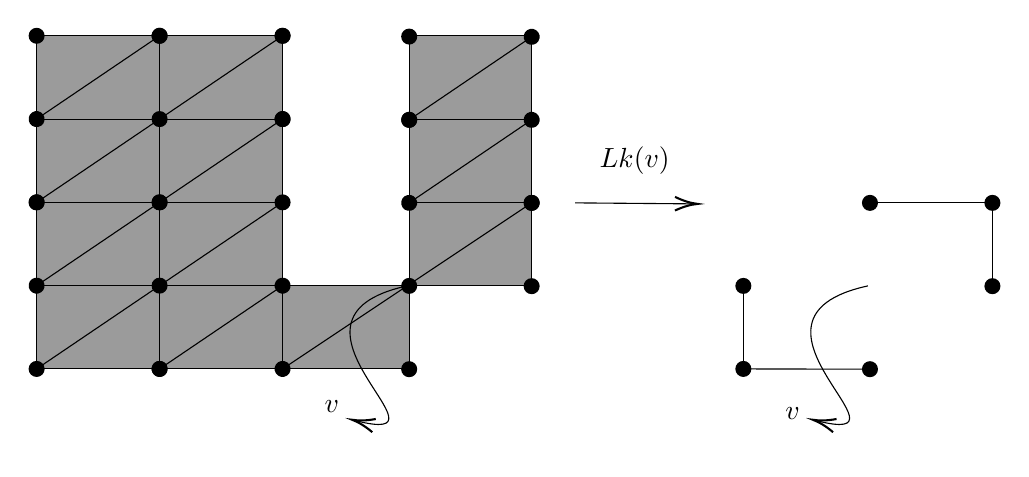
\begin{tikzpicture}[x=0.75pt,y=0.75pt,yscale=-1,xscale=1]
        %uncomment if require: \path (0,433); %set diagram left start at 0, and has height of 433

        %Shape: Rectangle [id:dp6828292052273273] 
        \draw  [fill={rgb, 255:red, 155; green, 155; blue, 155 }  ,fill opacity=1 ] (190.5,10) -- (249.5,10) -- (249.5,130.5) -- (190.5,130.5) -- cycle ;
        %Shape: Rectangle [id:dp1603709832259137] 
        \draw  [fill={rgb, 255:red, 155; green, 155; blue, 155 }  ,fill opacity=1 ] (190.5,50.25) -- (249.5,50.25) -- (249.5,90.25) -- (190.5,90.25) -- cycle ;
        %Shape: Rectangle [id:dp7801372435241032] 
        \draw  [fill={rgb, 255:red, 155; green, 155; blue, 155 }  ,fill opacity=1 ] (129.5,130.5) -- (190.5,130.5) -- (190.5,170.5) -- (129.5,170.5) -- cycle ;
        %Shape: Rectangle [id:dp29792580873182595] 
        \draw  [fill={rgb, 255:red, 155; green, 155; blue, 155 }  ,fill opacity=1 ] (190.5,90.5) -- (249.5,90.5) -- (249.5,130.5) -- (190.5,130.5) -- cycle ;
        %Shape: Rectangle [id:dp6639087811481719] 
        \draw  [fill={rgb, 255:red, 155; green, 155; blue, 155 }  ,fill opacity=1 ] (11,10) -- (129.5,10) -- (129.5,170.5) -- (11,170.5) -- cycle ;
        %Straight Lines [id:da6575867828932402] 
        \draw    (11,10) -- (11,170.5) ;
        %Straight Lines [id:da8065281350659392] 
        \draw    (11,10) -- (129.5,10) ;
        \draw [shift={(129.5,10)}, rotate = 0] [color={rgb, 255:red, 0; green, 0; blue, 0 }  ][fill={rgb, 255:red, 0; green, 0; blue, 0 }  ][line width=0.75]      (0, 0) circle [x radius= 3.35, y radius= 3.35]   ;
        \draw [shift={(11,10)}, rotate = 0] [color={rgb, 255:red, 0; green, 0; blue, 0 }  ][fill={rgb, 255:red, 0; green, 0; blue, 0 }  ][line width=0.75]      (0, 0) circle [x radius= 3.35, y radius= 3.35]   ;
        %Straight Lines [id:da3992609650184433] 
        \draw    (129.5,10) -- (129.5,170.5) ;
        %Straight Lines [id:da13475589884345496] 
        \draw    (11,170.5) -- (129.5,170.5) ;
        %Straight Lines [id:da4416095201662438] 
        \draw    (70.25,10) -- (70.25,170.5) ;
        \draw [shift={(70.25,170.5)}, rotate = 90] [color={rgb, 255:red, 0; green, 0; blue, 0 }  ][fill={rgb, 255:red, 0; green, 0; blue, 0 }  ][line width=0.75]      (0, 0) circle [x radius= 3.35, y radius= 3.35]   ;
        \draw [shift={(70.25,10)}, rotate = 90] [color={rgb, 255:red, 0; green, 0; blue, 0 }  ][fill={rgb, 255:red, 0; green, 0; blue, 0 }  ][line width=0.75]      (0, 0) circle [x radius= 3.35, y radius= 3.35]   ;
        %Straight Lines [id:da6740170575639275] 
        \draw    (11,90.25) -- (129.5,90.25) ;
        %Straight Lines [id:da719865308555645] 
        \draw    (129.5,10) -- (129.5,90.25) ;
        \draw [shift={(129.5,90.25)}, rotate = 90] [color={rgb, 255:red, 0; green, 0; blue, 0 }  ][fill={rgb, 255:red, 0; green, 0; blue, 0 }  ][line width=0.75]      (0, 0) circle [x radius= 3.35, y radius= 3.35]   ;
        \draw [shift={(129.5,10)}, rotate = 90] [color={rgb, 255:red, 0; green, 0; blue, 0 }  ][fill={rgb, 255:red, 0; green, 0; blue, 0 }  ][line width=0.75]      (0, 0) circle [x radius= 3.35, y radius= 3.35]   ;
        %Straight Lines [id:da7675296220139092] 
        \draw    (11,10) -- (11,90.25) ;
        %Straight Lines [id:da6604115448480403] 
        \draw    (129.5,90.25) -- (129.5,170.5) ;
        %Straight Lines [id:da921763560201903] 
        \draw    (11,90.25) -- (11,170.5) ;
        \draw [shift={(11,170.5)}, rotate = 90] [color={rgb, 255:red, 0; green, 0; blue, 0 }  ][fill={rgb, 255:red, 0; green, 0; blue, 0 }  ][line width=0.75]      (0, 0) circle [x radius= 3.35, y radius= 3.35]   ;
        \draw [shift={(11,90.25)}, rotate = 90] [color={rgb, 255:red, 0; green, 0; blue, 0 }  ][fill={rgb, 255:red, 0; green, 0; blue, 0 }  ][line width=0.75]      (0, 0) circle [x radius= 3.35, y radius= 3.35]   ;
        %Straight Lines [id:da8649318988296271] 
        \draw    (11,130.38) -- (129.5,130.38) ;
        %Straight Lines [id:da16660765957405133] 
        \draw    (11,50.13) -- (129.5,50.13) ;
        \draw [shift={(129.5,50.13)}, rotate = 0] [color={rgb, 255:red, 0; green, 0; blue, 0 }  ][fill={rgb, 255:red, 0; green, 0; blue, 0 }  ][line width=0.75]      (0, 0) circle [x radius= 3.35, y radius= 3.35]   ;
        %Straight Lines [id:da21493603049157772] 
        \draw    (70.25,10) -- (11,50.13) ;
        \draw [shift={(11,50.13)}, rotate = 145.89] [color={rgb, 255:red, 0; green, 0; blue, 0 }  ][fill={rgb, 255:red, 0; green, 0; blue, 0 }  ][line width=0.75]      (0, 0) circle [x radius= 3.35, y radius= 3.35]   ;
        \draw [shift={(70.25,10)}, rotate = 145.89] [color={rgb, 255:red, 0; green, 0; blue, 0 }  ][fill={rgb, 255:red, 0; green, 0; blue, 0 }  ][line width=0.75]      (0, 0) circle [x radius= 3.35, y radius= 3.35]   ;
        %Straight Lines [id:da018520940840161426] 
        \draw    (129.5,10) -- (11,90.25) ;
        \draw [shift={(11,90.25)}, rotate = 145.89] [color={rgb, 255:red, 0; green, 0; blue, 0 }  ][fill={rgb, 255:red, 0; green, 0; blue, 0 }  ][line width=0.75]      (0, 0) circle [x radius= 3.35, y radius= 3.35]   ;
        %Straight Lines [id:da8908508321424791] 
        \draw    (129.5,50.13) -- (11,130.38) ;
        \draw [shift={(11,130.38)}, rotate = 145.89] [color={rgb, 255:red, 0; green, 0; blue, 0 }  ][fill={rgb, 255:red, 0; green, 0; blue, 0 }  ][line width=0.75]      (0, 0) circle [x radius= 3.35, y radius= 3.35]   ;
        \draw [shift={(129.5,50.13)}, rotate = 145.89] [color={rgb, 255:red, 0; green, 0; blue, 0 }  ][fill={rgb, 255:red, 0; green, 0; blue, 0 }  ][line width=0.75]      (0, 0) circle [x radius= 3.35, y radius= 3.35]   ;
        %Straight Lines [id:da10224452058981259] 
        \draw    (129.5,90.25) -- (11,170.5) ;
        %Straight Lines [id:da8535884033018606] 
        \draw    (129.5,130.38) -- (70.25,170.5) ;
        \draw [shift={(70.25,170.5)}, rotate = 145.89] [color={rgb, 255:red, 0; green, 0; blue, 0 }  ][fill={rgb, 255:red, 0; green, 0; blue, 0 }  ][line width=0.75]      (0, 0) circle [x radius= 3.35, y radius= 3.35]   ;
        \draw [shift={(129.5,130.38)}, rotate = 145.89] [color={rgb, 255:red, 0; green, 0; blue, 0 }  ][fill={rgb, 255:red, 0; green, 0; blue, 0 }  ][line width=0.75]      (0, 0) circle [x radius= 3.35, y radius= 3.35]   ;
        %Straight Lines [id:da713065441573842] 
        \draw    (249.5,90.5) -- (129.5,170.5) ;
        \draw [shift={(129.5,170.5)}, rotate = 146.31] [color={rgb, 255:red, 0; green, 0; blue, 0 }  ][fill={rgb, 255:red, 0; green, 0; blue, 0 }  ][line width=0.75]      (0, 0) circle [x radius= 3.35, y radius= 3.35]   ;
        \draw [shift={(249.5,90.5)}, rotate = 146.31] [color={rgb, 255:red, 0; green, 0; blue, 0 }  ][fill={rgb, 255:red, 0; green, 0; blue, 0 }  ][line width=0.75]      (0, 0) circle [x radius= 3.35, y radius= 3.35]   ;
        %Straight Lines [id:da4858360870120242] 
        \draw    (190.5,90.5) -- (249.5,50.5) ;
        \draw [shift={(249.5,50.5)}, rotate = 325.86] [color={rgb, 255:red, 0; green, 0; blue, 0 }  ][fill={rgb, 255:red, 0; green, 0; blue, 0 }  ][line width=0.75]      (0, 0) circle [x radius= 3.35, y radius= 3.35]   ;
        \draw [shift={(190.5,90.5)}, rotate = 325.86] [color={rgb, 255:red, 0; green, 0; blue, 0 }  ][fill={rgb, 255:red, 0; green, 0; blue, 0 }  ][line width=0.75]      (0, 0) circle [x radius= 3.35, y radius= 3.35]   ;
        %Straight Lines [id:da10590665049175874] 
        \draw    (190.5,50.5) -- (249.5,10.5) ;
        \draw [shift={(249.5,10.5)}, rotate = 325.86] [color={rgb, 255:red, 0; green, 0; blue, 0 }  ][fill={rgb, 255:red, 0; green, 0; blue, 0 }  ][line width=0.75]      (0, 0) circle [x radius= 3.35, y radius= 3.35]   ;
        \draw [shift={(190.5,50.5)}, rotate = 325.86] [color={rgb, 255:red, 0; green, 0; blue, 0 }  ][fill={rgb, 255:red, 0; green, 0; blue, 0 }  ][line width=0.75]      (0, 0) circle [x radius= 3.35, y radius= 3.35]   ;
        %Curve Lines [id:da3048204937708163] 
        \draw    (189.5,130.5) .. controls (116.73,146.34) and (217.45,208.73) .. (164.65,195.43) ;
        \draw [shift={(163,195)}, rotate = 14.87] [color={rgb, 255:red, 0; green, 0; blue, 0 }  ][line width=0.75]    (10.93,-3.29) .. controls (6.95,-1.4) and (3.31,-0.3) .. (0,0) .. controls (3.31,0.3) and (6.95,1.4) .. (10.93,3.29)   ;
        %Straight Lines [id:da7015390425861685] 
        \draw    (270.5,90.5) -- (327.5,90.98) ;
        \draw [shift={(329.5,91)}, rotate = 180.49] [color={rgb, 255:red, 0; green, 0; blue, 0 }  ][line width=0.75]    (10.93,-3.29) .. controls (6.95,-1.4) and (3.31,-0.3) .. (0,0) .. controls (3.31,0.3) and (6.95,1.4) .. (10.93,3.29)   ;
        %Straight Lines [id:da7996705859516942] 
        \draw    (70.25,90.25) -- (70.25,130.38) ;
        \draw [shift={(70.25,130.38)}, rotate = 90] [color={rgb, 255:red, 0; green, 0; blue, 0 }  ][fill={rgb, 255:red, 0; green, 0; blue, 0 }  ][line width=0.75]      (0, 0) circle [x radius= 3.35, y radius= 3.35]   ;
        \draw [shift={(70.25,90.25)}, rotate = 90] [color={rgb, 255:red, 0; green, 0; blue, 0 }  ][fill={rgb, 255:red, 0; green, 0; blue, 0 }  ][line width=0.75]      (0, 0) circle [x radius= 3.35, y radius= 3.35]   ;
        %Straight Lines [id:da3138524723474039] 
        \draw    (70.25,50.13) -- (70.25,90.25) ;
        \draw [shift={(70.25,90.25)}, rotate = 90] [color={rgb, 255:red, 0; green, 0; blue, 0 }  ][fill={rgb, 255:red, 0; green, 0; blue, 0 }  ][line width=0.75]      (0, 0) circle [x radius= 3.35, y radius= 3.35]   ;
        \draw [shift={(70.25,50.13)}, rotate = 90] [color={rgb, 255:red, 0; green, 0; blue, 0 }  ][fill={rgb, 255:red, 0; green, 0; blue, 0 }  ][line width=0.75]      (0, 0) circle [x radius= 3.35, y radius= 3.35]   ;
        %Straight Lines [id:da6901146317341891] 
        \draw    (190.5,130.5) -- (190.5,170.63) ;
        \draw [shift={(190.5,170.63)}, rotate = 90] [color={rgb, 255:red, 0; green, 0; blue, 0 }  ][fill={rgb, 255:red, 0; green, 0; blue, 0 }  ][line width=0.75]      (0, 0) circle [x radius= 3.35, y radius= 3.35]   ;
        \draw [shift={(190.5,130.5)}, rotate = 90] [color={rgb, 255:red, 0; green, 0; blue, 0 }  ][fill={rgb, 255:red, 0; green, 0; blue, 0 }  ][line width=0.75]      (0, 0) circle [x radius= 3.35, y radius= 3.35]   ;
        %Straight Lines [id:da5863145317047915] 
        \draw    (190.5,10.38) -- (190.5,50.5) ;
        \draw [shift={(190.5,50.5)}, rotate = 90] [color={rgb, 255:red, 0; green, 0; blue, 0 }  ][fill={rgb, 255:red, 0; green, 0; blue, 0 }  ][line width=0.75]      (0, 0) circle [x radius= 3.35, y radius= 3.35]   ;
        \draw [shift={(190.5,10.38)}, rotate = 90] [color={rgb, 255:red, 0; green, 0; blue, 0 }  ][fill={rgb, 255:red, 0; green, 0; blue, 0 }  ][line width=0.75]      (0, 0) circle [x radius= 3.35, y radius= 3.35]   ;
        %Straight Lines [id:da15956690296671794] 
        \draw    (249.5,90.5) -- (249.5,130.63) ;
        \draw [shift={(249.5,130.63)}, rotate = 90] [color={rgb, 255:red, 0; green, 0; blue, 0 }  ][fill={rgb, 255:red, 0; green, 0; blue, 0 }  ][line width=0.75]      (0, 0) circle [x radius= 3.35, y radius= 3.35]   ;
        \draw [shift={(249.5,90.5)}, rotate = 90] [color={rgb, 255:red, 0; green, 0; blue, 0 }  ][fill={rgb, 255:red, 0; green, 0; blue, 0 }  ][line width=0.75]      (0, 0) circle [x radius= 3.35, y radius= 3.35]   ;
        %Straight Lines [id:da5644396890713788] 
        \draw    (471.5,90.5) -- (471.5,130.63) ;
        \draw [shift={(471.5,130.63)}, rotate = 90] [color={rgb, 255:red, 0; green, 0; blue, 0 }  ][fill={rgb, 255:red, 0; green, 0; blue, 0 }  ][line width=0.75]      (0, 0) circle [x radius= 3.35, y radius= 3.35]   ;
        \draw [shift={(471.5,90.5)}, rotate = 90] [color={rgb, 255:red, 0; green, 0; blue, 0 }  ][fill={rgb, 255:red, 0; green, 0; blue, 0 }  ][line width=0.75]      (0, 0) circle [x radius= 3.35, y radius= 3.35]   ;
        %Curve Lines [id:da05898074275878096] 
        \draw    (411.5,130.5) .. controls (338.73,146.34) and (439.45,208.73) .. (386.65,195.43) ;
        \draw [shift={(385,195)}, rotate = 14.87] [color={rgb, 255:red, 0; green, 0; blue, 0 }  ][line width=0.75]    (10.93,-3.29) .. controls (6.95,-1.4) and (3.31,-0.3) .. (0,0) .. controls (3.31,0.3) and (6.95,1.4) .. (10.93,3.29)   ;
        %Straight Lines [id:da8439868174235072] 
        \draw    (351.5,170.5) -- (412.5,170.63) ;
        \draw [shift={(412.5,170.63)}, rotate = 0.12] [color={rgb, 255:red, 0; green, 0; blue, 0 }  ][fill={rgb, 255:red, 0; green, 0; blue, 0 }  ][line width=0.75]      (0, 0) circle [x radius= 3.35, y radius= 3.35]   ;
        %Straight Lines [id:da8450303037567879] 
        \draw    (351.5,130.5) -- (351.5,170.5) ;
        \draw [shift={(351.5,170.5)}, rotate = 90] [color={rgb, 255:red, 0; green, 0; blue, 0 }  ][fill={rgb, 255:red, 0; green, 0; blue, 0 }  ][line width=0.75]      (0, 0) circle [x radius= 3.35, y radius= 3.35]   ;
        \draw [shift={(351.5,130.5)}, rotate = 90] [color={rgb, 255:red, 0; green, 0; blue, 0 }  ][fill={rgb, 255:red, 0; green, 0; blue, 0 }  ][line width=0.75]      (0, 0) circle [x radius= 3.35, y radius= 3.35]   ;
        %Straight Lines [id:da13676375427748955] 
        \draw    (471.5,90.5) -- (412.5,90.5) ;
        \draw [shift={(412.5,90.5)}, rotate = 180] [color={rgb, 255:red, 0; green, 0; blue, 0 }  ][fill={rgb, 255:red, 0; green, 0; blue, 0 }  ][line width=0.75]      (0, 0) circle [x radius= 3.35, y radius= 3.35]   ;

        % Text Node
        \draw (148.5,184.4) node [anchor=north west][inner sep=0.75pt]    {$v$};
        % Text Node
        \draw (281,62.4) node [anchor=north west][inner sep=0.75pt]    {$Lk( v)$};
        % Text Node
        \draw (370.5,187.9) node [anchor=north west][inner sep=0.75pt]    {$v$};


    \end{tikzpicture}

\end{center}
\begin{definition}[Mappa simpliciale]
    Siano $K$ e $L$ due complessi simpliciali e sia
    \[
        f:\pskel{K}{0}\ra\pskel{L}{0}
    \]
    una funzione tale che per ogni insieme di vertici \pointset di $K$ che generano un simplesso di $K$, i punti corrispondenti
    \[
        \{f(P_0),f(P_1),\dots,f(P_K)\}
    \]
    devono essere vertici di un simplesso di $L$.\\
    Allora la funzione $f$ si può estendere ad una funzione continua
    \[
        \tilde{f}:|K|\ra|L|
    \]
    tale che
    \[
        x\in\sigma\in K\quad x=\sum_{i=0}^k t_iP_i\quad \tilde{f}(x)=\sum_{i=0}^k t_if(P_i)
    \]
    Chiamiamo $\tilde{f}$ mappa simpliciale (lineare) indotta da $f$
\end{definition}
\paragraph{Osservazione} Per ogni $x\in|K|$, esiste un unico $\sigma\in K$ tale che $x$ sia un punto della parte interna di $\sigma$
\paragraph{Osservazione} Non stiamo chiedendo che i punti che otteniamo siano distinti
\pagebreak
\paragraph{Esempio 1}
\begin{center}


    \tikzset{every picture/.style={line width=0.75pt}} %set default line width to 0.75pt        

    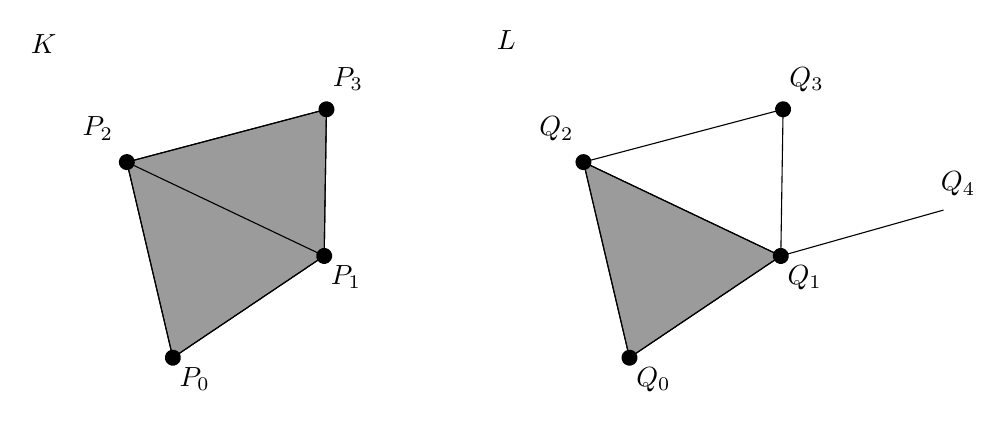
\begin{tikzpicture}[x=0.75pt,y=0.75pt,yscale=-1,xscale=1]
        %uncomment if require: \path (0,433); %set diagram left start at 0, and has height of 433

        %Shape: Polygon [id:ds6404447644709921] 
        \draw  [fill={rgb, 255:red, 155; green, 155; blue, 155 }  ,fill opacity=1 ] (159.19,44.96) -- (158.09,115.61) -- (85.19,164.63) -- (63.01,70.4) -- cycle ;
        %Straight Lines [id:da531965220828956] 
        \draw    (63.01,70.4) -- (158.09,115.61) ;
        \draw [shift={(63.01,70.4)}, rotate = 25.43] [color={rgb, 255:red, 0; green, 0; blue, 0 }  ][fill={rgb, 255:red, 0; green, 0; blue, 0 }  ][line width=0.75]      (0, 0) circle [x radius= 3.35, y radius= 3.35]   ;
        %Straight Lines [id:da7690113746306688] 
        \draw    (63.01,70.4) -- (159.19,44.96) ;
        \draw [shift={(159.19,44.96)}, rotate = 345.19] [color={rgb, 255:red, 0; green, 0; blue, 0 }  ][fill={rgb, 255:red, 0; green, 0; blue, 0 }  ][line width=0.75]      (0, 0) circle [x radius= 3.35, y radius= 3.35]   ;
        %Straight Lines [id:da7289165213757174] 
        \draw    (159.19,44.96) -- (158.09,115.61) ;
        %Straight Lines [id:da3093984357313633] 
        \draw    (158.09,115.61) -- (85.19,164.63) ;
        \draw [shift={(85.19,164.63)}, rotate = 146.08] [color={rgb, 255:red, 0; green, 0; blue, 0 }  ][fill={rgb, 255:red, 0; green, 0; blue, 0 }  ][line width=0.75]      (0, 0) circle [x radius= 3.35, y radius= 3.35]   ;
        \draw [shift={(158.09,115.61)}, rotate = 146.08] [color={rgb, 255:red, 0; green, 0; blue, 0 }  ][fill={rgb, 255:red, 0; green, 0; blue, 0 }  ][line width=0.75]      (0, 0) circle [x radius= 3.35, y radius= 3.35]   ;
        %Straight Lines [id:da9033353416862113] 
        \draw    (63.01,70.4) -- (85.19,164.63) ;

        %Shape: Polygon [id:ds7686101763709159] 
        \draw  [fill={rgb, 255:red, 155; green, 155; blue, 155 }  ,fill opacity=1 ] (378.09,115.61) -- (305.19,164.63) -- (283.01,70.4) -- cycle ;
        %Straight Lines [id:da41241768674383605] 
        \draw    (283.01,70.4) -- (378.09,115.61) ;
        \draw [shift={(283.01,70.4)}, rotate = 25.43] [color={rgb, 255:red, 0; green, 0; blue, 0 }  ][fill={rgb, 255:red, 0; green, 0; blue, 0 }  ][line width=0.75]      (0, 0) circle [x radius= 3.35, y radius= 3.35]   ;
        %Straight Lines [id:da12420673174050467] 
        \draw    (283.01,70.4) -- (379.19,44.96) ;
        \draw [shift={(379.19,44.96)}, rotate = 345.19] [color={rgb, 255:red, 0; green, 0; blue, 0 }  ][fill={rgb, 255:red, 0; green, 0; blue, 0 }  ][line width=0.75]      (0, 0) circle [x radius= 3.35, y radius= 3.35]   ;
        %Straight Lines [id:da1245706573751042] 
        \draw    (379.19,44.96) -- (378.09,115.61) ;
        %Straight Lines [id:da4772692294819698] 
        \draw    (378.09,115.61) -- (305.19,164.63) ;
        \draw [shift={(305.19,164.63)}, rotate = 146.08] [color={rgb, 255:red, 0; green, 0; blue, 0 }  ][fill={rgb, 255:red, 0; green, 0; blue, 0 }  ][line width=0.75]      (0, 0) circle [x radius= 3.35, y radius= 3.35]   ;
        \draw [shift={(378.09,115.61)}, rotate = 146.08] [color={rgb, 255:red, 0; green, 0; blue, 0 }  ][fill={rgb, 255:red, 0; green, 0; blue, 0 }  ][line width=0.75]      (0, 0) circle [x radius= 3.35, y radius= 3.35]   ;
        %Straight Lines [id:da28332688532397654] 
        \draw    (283.01,70.4) -- (305.19,164.63) ;

        %Straight Lines [id:da47886677319122084] 
        \draw    (378.09,115.61) -- (456.5,93.5) ;

        % Text Node
        \draw (87.19,168.03) node [anchor=north west][inner sep=0.75pt]    {$P_{0}$};
        % Text Node
        \draw (160.09,119.01) node [anchor=north west][inner sep=0.75pt]    {$P_{1}$};
        % Text Node
        \draw (40.5,47.4) node [anchor=north west][inner sep=0.75pt]    {$P_{2}$};
        % Text Node
        \draw (161,23.4) node [anchor=north west][inner sep=0.75pt]    {$P_{3}$};
        % Text Node
        \draw (15.5,7.9) node [anchor=north west][inner sep=0.75pt]    {$K$};
        % Text Node
        \draw (307.19,168.03) node [anchor=north west][inner sep=0.75pt]    {$Q_{0}$};
        % Text Node
        \draw (380.09,119.01) node [anchor=north west][inner sep=0.75pt]    {$Q_{1}$};
        % Text Node
        \draw (260.5,47.4) node [anchor=north west][inner sep=0.75pt]    {$Q_{2}$};
        % Text Node
        \draw (381,23.4) node [anchor=north west][inner sep=0.75pt]    {$Q_{3}$};
        % Text Node
        \draw (240,5.9) node [anchor=north west][inner sep=0.75pt]    {$L$};
        % Text Node
        \draw (454,73.9) node [anchor=north west][inner sep=0.75pt]    {$Q_{4}$};


    \end{tikzpicture}

\end{center}
Consideriamo la funzione
\[
    f:\pskel{K}{0}\ra\pskel{L}{0}
\]
definita come
\[
    P_0\longmapsto Q_0\quad P_1\longmapsto Q_1
\]
\[
    P_2\longmapsto Q_2 \text{ oppure } P_2\longmapsto Q_0 \text{ oppure }P_2\longmapsto Q_1
\]
\[
    x\in[P_0,P_1,P_2]\implies x=t_0P_0+t_1P_1+t_2P_2
\]
\begin{enumerate}
    \item[Caso 1)]
        \[
            \tilde{f}(x)=t_0f(P_0)+t_1f(P_1)+t_2f(P_2)=t_0Q_0+_1Q_1+t_2Q_2\in[Q_0,Q_1,Q_2]
        \]
    \item[Caso 2/3)]
        \[
            \tilde{f}(x)=t_0f(P_0)+t_1f(P_1)+t_2f(P_2)=(t_0+t_2)Q_0+t_1Q_1\in[Q_0,Q_1]
        \]
\end{enumerate}
\paragraph{Esempio 2} Un esempio di funzione che non si esteda a una mappa simpliciale è
\[
    P_0\longmapsto Q_1\quad P_1\longmapsto Q_1\quad P_2\longmapsto Q_2
\]
\[
    P_3\longmapsto Q_3\text{ oppure }P_3\longmapsto Q_4
\]
$\{P_1,P_2,P_3\}$ generano un 2-simplesso di $K$, ma
\[
    \{f(P_1),f(P_2),f(P_3)\}=\{Q_1,Q_2,Q_3\}
\]
non sono vertici di un simplesso di $L$
\paragraph{Utilità}
Questa possibilità permette di dimostrare che la composizione di mappe simpliciali è una mappa simpliciale
\[\begin{tikzcd}
        {K^{(0)}} && {L^{(0)}} && {M^{(0)}}
        \arrow["f", from=1-1, to=1-3]
        \arrow["g", from=1-3, to=1-5]
        \arrow["{g\circ f}"', curve={height=30pt}, from=1-1, to=1-5]
    \end{tikzcd}\]
\[
    x=\sum_{i=0}^k t_iP_i\mapsto\tilde{f}(x)=\sum_{i=0}^k t_if(P_i)\mapsto\tilde{g}(\tilde{f}(x))=\sum_{i=0}^kt_ig(f(P_i))
\]
\paragraph{Osservazione} $\tilde{f}:|K|\ra|L|$ è continua, ossia $\left.\tilde{f}\right|_\sigma:\sigma\ra|L|$ è continua $\forall\sigma\in K$
\[
    \sigma=[P_0,\dots,P_k]\overset{\tilde{f}}{\longmapsto}[f(P_0),\dots,f(P_k)]
\]
è continua poichè è una mappa di inclusione
\[
    i:[f(P_0),\dots,f(P_k)]\hookrightarrow|L|
\]
\begin{proposition}
    Siano $K$ e $L$ due complessi simpliciali e sia $f:\pskel{K}{0}\ra\pskel{L}{0}$ una funzione biettiva tale che i vertici $P_0,\dots,P_k\in\pskel{K}{0}$ generano un simplesso di $K$ se e solo se $f(P_0),\dots,f(P_k)\in\pskel{L}{0}$ generano un simplesso di $L$.\\
    Allora la mappa simpliciale indotta $\tilde{f}:|K|\ra|L|$ è un omeomorfismo
\end{proposition}
\begin{proof}
    Se $f:\pskel{K}{0}\ra\pskel{L}{0}$ è biettiva, allora $\exists g:\pskel{L}{0}\ra\pskel{K}{0}$ tale che
    \[
        g\circ f=f\circ g=id
    \]
    quindi $g=f^{-1}$. Segue che
    \[
        \tilde{f}^{-1}\left(\tilde{f}(x)\right)=\tilde{f}^{-1}\left(\sum_{i=0}^kt_if(P_i)\right)=\sum_{i=0}^k t_if^{-1}\left(f(P_i)\right)=\sum_{i=0}^k t_iP_i=x
    \]
\end{proof}
\paragraph{Corollario} Condizioni necessarie per essere omeomorfismi via mappe simpliciali
\begin{itemize}
    \item $K$ finito, $|K|$ compatto, e $|L|,|K|$ omeomoerfi (via m.s.) $\implies$ $L$ finito, $|L|$ compatto
    \item $|K|$ $|L|$ omeomorfi $\implies$ \pskel{K}{0} e \pskel{L}{0} hanno la stessa cardinalità
    \item $|K|$ $|L|$ omeomorfi $\implies$ $K$ e $L$ hanno lo stesso numero di p-simplessi $\forall p$
\end{itemize}
\begin{corollary}
    Sia $K$ un complesso simpliciale finito, allor $|K|$ è omeomorfo allo spazio soggiacente di un sottocomplesso del complesso simpliciale formato dal simplesso standard $\Delta^N$ con le sue facce, per un $N$ sufficentemente grande
\end{corollary}
\begin{proof}
    Prendiamo $P_0,\dots,P_n$ vertici di $K$, i vertici del simplesso standard $\Delta^N$ sono
    \[
        \left\{0,\underline{e_1},\underline{e_2},\dots,\underline{e_n},\right\}
    \]
    Prendiamo la funzione
    \[
        f:\pskel{K}{0}\ra\Delta^{N^{(0)}}
    \]
    che associa
    \[
        P_0\longmapsto\underline{0}
    \]
    \[
        P_i\longmapsto\underline{e_i}
    \]
    Il sottocomplesso $L\subset\Delta^N$ con spazio soggiacente omeomorfo a $|K|$ è
    \[
        L=\setst{\sigma\in\Delta^N}{\sigma=[f(P_0),\dots,f(P_k)]}
    \]
    per $[P_0,\dots,P_k]\in K$
\end{proof}
\chapter{Complessi simpliciali astratti}
Abbiamo quindi visto come l'omomorfismo topologico è controllato completamente dalle proprietà combinatoriali, e non da quelle geometriche.\\
Inoltre, le coordinate dei vertici non influiscono sugli enunciati e sui teoremi, ma quello che conta è la struttura astratta. Possiamo quindi dare una struttura algebrica più raffinata ai complessi simpliciali.
\begin{definition}[Complesso simpliciale astratto]
    Un complesso simpliciale astratto è una collezione $\mathcal{S}$ di insiemi finiti non vuoti tali che
    \[
        A\in\mathcal{S}\implies\powerset(A)\in\mathcal{S}
    \]
\end{definition}
\paragraph{Nomenclatura} Abbiamo una equivalenza tra la nomenclatura dei complessi simpliciali geometrici e dei complessi simpliciali astratti
\begin{itemize}
    \item Ogni $A\in\mathcal{S}$ si dice simplesso astratto
    \item La dimensione di $A\in\mathcal{S}$ è pari al numero di elementi meno 1
    \item Ogni sottoinsieme di $A\in\mathcal{S}$ si dice faccia di $A$
    \item La mensione di $\mathcal{S}$ è la dimensione massima di un suo sottoinsieme
    \item L'insieme dei vertici di $\mathcal{S}$ (l'insieme dei singoletti) si dice 0-scheletro di $\mathcal{S}$, l'insieme dei sottoinsiemi di 1 elemento si dice 1-scheletro di $\mathcal{S}$ ecc.
    \item Due complessi simpliciali astratti $\mathcal{S}$ e $\mathcal{T}$ si dicono isomorfi se c'è una corrispondenza biunivoca tra gli 0-scheletri tale che
          \[
              \{a_0,a_1,\dots,a_k\}\in\mathcal{S}\Longleftrightarrow \{f(a_0),f(a_1),\dots,f(a_k)\}\in\mathcal{T}
          \]
\end{itemize}
\pagebreak
\begin{definition}[Vertex scheme]
    Sia $K$ un complesso simpliciale (geometrico) e sia $V=\pskel{K}{0}$ l'insieme dei vertici di $K$.\\
    La collezione di sottoinsiemi di $V$
    \[
        \mathcal{K}:=\setst{\{v_0,v_1,\dots,v_k\}\in V}{[v_0,\dots,v_n]\in K}
    \]
    è un complesso simplicale astratto detto vertex scheme di $K$
\end{definition}
\begin{theorem}
    \begin{itemize}
        \item Ogni complesso simpliciale astratto è isomorof ad un vertex scheme di un complesso simpliciale geometrico
        \item Due complessi simpliciali (geometrici) sono isomorfi (e gli spazi soggiacenti omeomorfi) se e solo se i vertex scheme sono isomorfi
    \end{itemize}
\end{theorem}
\pagebreak
\paragraph{Esempio}
Consideriamo il complesso simpliciale astratto
\[
    S=\left\{
    \begin{array}{l}
        \{0,1,2\},\{0,1,4\},\{0,2,3\},\{0,3,4\},\{1,2,5\},\{1,4,5\}, \\
        \{2,3,5\},\{3,4,5\},\text{e tutti i sottoinsiemi}
    \end{array}
    \right\}
\]
Qual'è il complesso simpliciale geometrico che ha $S$ come vertex scheme?
\begin{center}


    \tikzset{every picture/.style={line width=0.75pt}} %set default line width to 0.75pt        

    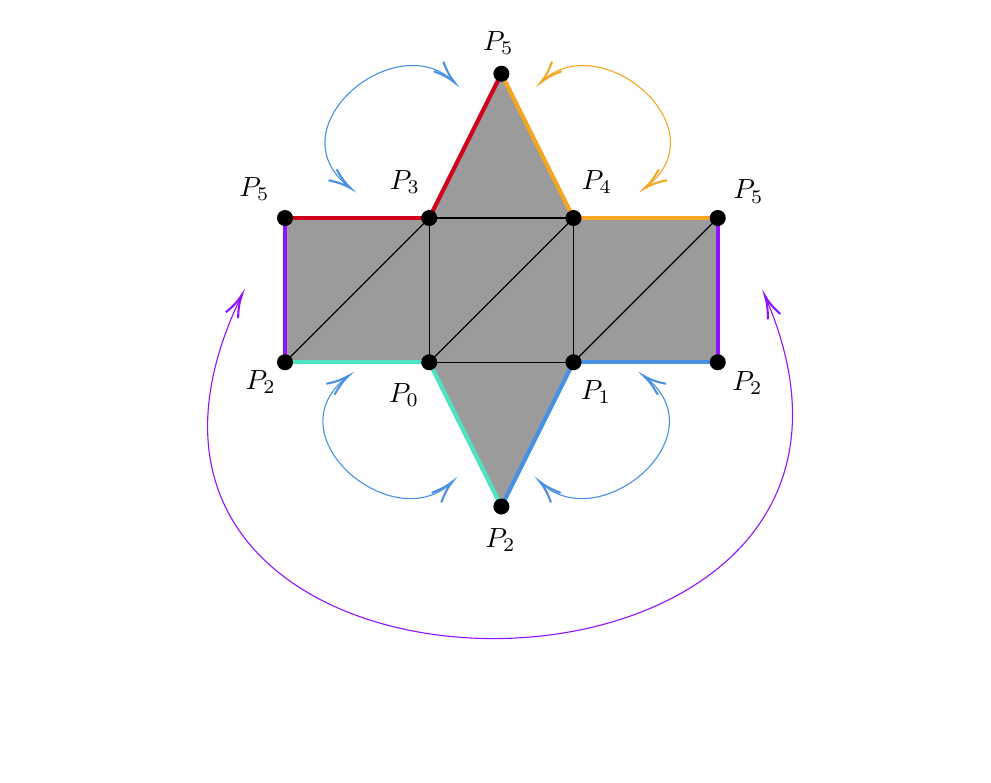
\begin{tikzpicture}[x=0.75pt,y=0.75pt,yscale=-1,xscale=1]
        %uncomment if require: \path (0,433); %set diagram left start at 0, and has height of 433

        %Shape: Polygon [id:ds8975669818370895] 
        \draw  [fill={rgb, 255:red, 155; green, 155; blue, 155 }  ,fill opacity=1 ] (313.5,172.5) -- (244,172.5) -- (244,126) -- (244,103) -- (313.5,103) -- (348.25,33.5) -- (383,103) -- (452.5,103) -- (452.5,172.5) -- (383,172.5) -- (348.25,242) -- cycle ;
        %Shape: Rectangle [id:dp8501380531139862] 
        \draw   (244,103) -- (313.5,103) -- (313.5,172.5) -- (244,172.5) -- cycle ;
        %Shape: Rectangle [id:dp9942000382671217] 
        \draw   (313.5,103) -- (383,103) -- (383,172.5) -- (313.5,172.5) -- cycle ;
        %Shape: Rectangle [id:dp5207030249538354] 
        \draw   (383,103) -- (452.5,103) -- (452.5,172.5) -- (383,172.5) -- cycle ;
        %Straight Lines [id:da17302255236904318] 
        \draw [color={rgb, 255:red, 208; green, 2; blue, 27 }  ,draw opacity=1 ][line width=1.5]    (244,103) -- (313.5,103) ;
        %Straight Lines [id:da7495218417557872] 
        \draw [color={rgb, 255:red, 144; green, 19; blue, 254 }  ,draw opacity=1 ][line width=1.5]    (452.5,103) -- (452.5,172.5) ;
        %Straight Lines [id:da5765541853301017] 
        \draw [color={rgb, 255:red, 208; green, 2; blue, 27 }  ,draw opacity=1 ][line width=1.5]    (313.5,103) -- (348.25,33.5) ;
        %Straight Lines [id:da23830409202348912] 
        \draw [color={rgb, 255:red, 74; green, 144; blue, 226 }  ,draw opacity=1 ][line width=1.5]    (383,172.5) -- (348.25,242) ;
        %Straight Lines [id:da17520600867325076] 
        \draw [color={rgb, 255:red, 80; green, 227; blue, 194 }  ,draw opacity=1 ][line width=1.5]    (313.5,172.5) -- (348.25,242) ;
        %Curve Lines [id:da0019052146436389084] 
        \draw [color={rgb, 255:red, 74; green, 144; blue, 226 }  ,draw opacity=1 ]   (418.49,180.36) .. controls (436.44,195.13) and (429.5,215.15) .. (414.79,227.34) .. controls (401.4,238.44) and (381.57,243.05) .. (368.18,231.34) ;
        \draw [shift={(366.75,230)}, rotate = 45] [color={rgb, 255:red, 74; green, 144; blue, 226 }  ,draw opacity=1 ][line width=0.75]    (10.93,-3.29) .. controls (6.95,-1.4) and (3.31,-0.3) .. (0,0) .. controls (3.31,0.3) and (6.95,1.4) .. (10.93,3.29)   ;
        \draw [shift={(416.75,179)}, rotate = 36.51] [color={rgb, 255:red, 74; green, 144; blue, 226 }  ,draw opacity=1 ][line width=0.75]    (10.93,-3.29) .. controls (6.95,-1.4) and (3.31,-0.3) .. (0,0) .. controls (3.31,0.3) and (6.95,1.4) .. (10.93,3.29)   ;
        %Straight Lines [id:da5132325967883811] 
        \draw [color={rgb, 255:red, 245; green, 166; blue, 35 }  ,draw opacity=1 ][line width=1.5]    (383,103) -- (348.25,33.5) ;
        %Straight Lines [id:da1753899770952616] 
        \draw [color={rgb, 255:red, 245; green, 166; blue, 35 }  ,draw opacity=1 ][line width=1.5]    (383,103) -- (452.5,103) ;
        %Straight Lines [id:da2593613204288545] 
        \draw [color={rgb, 255:red, 144; green, 19; blue, 254 }  ,draw opacity=1 ][line width=1.5]    (244,103) -- (244,172.5) ;
        %Straight Lines [id:da8504600910817144] 
        \draw [color={rgb, 255:red, 80; green, 227; blue, 194 }  ,draw opacity=1 ][line width=1.5]    (244,172.5) -- (313.5,172.5) ;
        %Straight Lines [id:da039973041394031794] 
        \draw [color={rgb, 255:red, 74; green, 144; blue, 226 }  ,draw opacity=1 ][line width=1.5]    (383,172.5) -- (452.5,172.5) ;
        %Straight Lines [id:da6892127503064209] 
        \draw    (244,172.5) -- (313.5,103) ;
        \draw [shift={(313.5,103)}, rotate = 315] [color={rgb, 255:red, 0; green, 0; blue, 0 }  ][fill={rgb, 255:red, 0; green, 0; blue, 0 }  ][line width=0.75]      (0, 0) circle [x radius= 3.35, y radius= 3.35]   ;
        \draw [shift={(244,172.5)}, rotate = 315] [color={rgb, 255:red, 0; green, 0; blue, 0 }  ][fill={rgb, 255:red, 0; green, 0; blue, 0 }  ][line width=0.75]      (0, 0) circle [x radius= 3.35, y radius= 3.35]   ;
        %Straight Lines [id:da5948963365159696] 
        \draw    (313.5,172.5) -- (383,103) ;
        \draw [shift={(383,103)}, rotate = 315] [color={rgb, 255:red, 0; green, 0; blue, 0 }  ][fill={rgb, 255:red, 0; green, 0; blue, 0 }  ][line width=0.75]      (0, 0) circle [x radius= 3.35, y radius= 3.35]   ;
        \draw [shift={(313.5,172.5)}, rotate = 315] [color={rgb, 255:red, 0; green, 0; blue, 0 }  ][fill={rgb, 255:red, 0; green, 0; blue, 0 }  ][line width=0.75]      (0, 0) circle [x radius= 3.35, y radius= 3.35]   ;
        %Straight Lines [id:da21980568120437005] 
        \draw    (383,172.5) -- (452.5,103) ;
        \draw [shift={(452.5,103)}, rotate = 315] [color={rgb, 255:red, 0; green, 0; blue, 0 }  ][fill={rgb, 255:red, 0; green, 0; blue, 0 }  ][line width=0.75]      (0, 0) circle [x radius= 3.35, y radius= 3.35]   ;
        \draw [shift={(383,172.5)}, rotate = 315] [color={rgb, 255:red, 0; green, 0; blue, 0 }  ][fill={rgb, 255:red, 0; green, 0; blue, 0 }  ][line width=0.75]      (0, 0) circle [x radius= 3.35, y radius= 3.35]   ;
        %Straight Lines [id:da7623743738803848] 
        \draw    (244,103) ;
        \draw [shift={(244,103)}, rotate = 0] [color={rgb, 255:red, 0; green, 0; blue, 0 }  ][fill={rgb, 255:red, 0; green, 0; blue, 0 }  ][line width=0.75]      (0, 0) circle [x radius= 3.35, y radius= 3.35]   ;
        %Straight Lines [id:da7357598169013839] 
        \draw    (348.25,242) ;
        \draw [shift={(348.25,242)}, rotate = 0] [color={rgb, 255:red, 0; green, 0; blue, 0 }  ][fill={rgb, 255:red, 0; green, 0; blue, 0 }  ][line width=0.75]      (0, 0) circle [x radius= 3.35, y radius= 3.35]   ;
        %Straight Lines [id:da8022976959499744] 
        \draw    (452.5,172.5) ;
        \draw [shift={(452.5,172.5)}, rotate = 0] [color={rgb, 255:red, 0; green, 0; blue, 0 }  ][fill={rgb, 255:red, 0; green, 0; blue, 0 }  ][line width=0.75]      (0, 0) circle [x radius= 3.35, y radius= 3.35]   ;
        %Straight Lines [id:da3049063743465379] 
        \draw    (348.25,33.5) ;
        \draw [shift={(348.25,33.5)}, rotate = 0] [color={rgb, 255:red, 0; green, 0; blue, 0 }  ][fill={rgb, 255:red, 0; green, 0; blue, 0 }  ][line width=0.75]      (0, 0) circle [x radius= 3.35, y radius= 3.35]   ;
        %Shape: Boxed Bezier Curve [id:dp9130104178425995] 
        \draw [color={rgb, 255:red, 74; green, 144; blue, 226 }  ,draw opacity=1 ]   (273.04,180.3) .. controls (238.54,208.57) and (295.37,256.13) .. (323.44,231.19) ;
        \draw [shift={(324.7,230)}, rotate = 135] [color={rgb, 255:red, 74; green, 144; blue, 226 }  ,draw opacity=1 ][line width=0.75]    (10.93,-3.29) .. controls (6.95,-1.4) and (3.31,-0.3) .. (0,0) .. controls (3.31,0.3) and (6.95,1.4) .. (10.93,3.29)   ;
        \draw [shift={(274.7,179)}, rotate = 143.49] [color={rgb, 255:red, 74; green, 144; blue, 226 }  ,draw opacity=1 ][line width=0.75]    (10.93,-3.29) .. controls (6.95,-1.4) and (3.31,-0.3) .. (0,0) .. controls (3.31,0.3) and (6.95,1.4) .. (10.93,3.29)   ;
        %Curve Lines [id:da2158833564972651] 
        \draw [color={rgb, 255:red, 245; green, 166; blue, 35 }  ,draw opacity=1 ]   (418.99,87.33) .. controls (436.94,72.56) and (430,52.54) .. (415.29,40.35) .. controls (401.9,29.25) and (382.07,24.64) .. (368.68,36.35) ;
        \draw [shift={(367.25,37.69)}, rotate = 315] [color={rgb, 255:red, 245; green, 166; blue, 35 }  ,draw opacity=1 ][line width=0.75]    (10.93,-3.29) .. controls (6.95,-1.4) and (3.31,-0.3) .. (0,0) .. controls (3.31,0.3) and (6.95,1.4) .. (10.93,3.29)   ;
        \draw [shift={(417.25,88.69)}, rotate = 323.49] [color={rgb, 255:red, 245; green, 166; blue, 35 }  ,draw opacity=1 ][line width=0.75]    (10.93,-3.29) .. controls (6.95,-1.4) and (3.31,-0.3) .. (0,0) .. controls (3.31,0.3) and (6.95,1.4) .. (10.93,3.29)   ;
        %Shape: Boxed Bezier Curve [id:dp2146720722641542] 
        \draw [color={rgb, 255:red, 74; green, 144; blue, 226 }  ,draw opacity=1 ]   (274.04,87.39) .. controls (239.54,59.12) and (296.37,11.56) .. (324.44,36.5) ;
        \draw [shift={(325.7,37.69)}, rotate = 225] [color={rgb, 255:red, 74; green, 144; blue, 226 }  ,draw opacity=1 ][line width=0.75]    (10.93,-3.29) .. controls (6.95,-1.4) and (3.31,-0.3) .. (0,0) .. controls (3.31,0.3) and (6.95,1.4) .. (10.93,3.29)   ;
        \draw [shift={(275.7,88.69)}, rotate = 216.51] [color={rgb, 255:red, 74; green, 144; blue, 226 }  ,draw opacity=1 ][line width=0.75]    (10.93,-3.29) .. controls (6.95,-1.4) and (3.31,-0.3) .. (0,0) .. controls (3.31,0.3) and (6.95,1.4) .. (10.93,3.29)   ;
        %Curve Lines [id:da9140193308226627] 
        \draw [color={rgb, 255:red, 144; green, 19; blue, 254 }  ,draw opacity=1 ]   (221.68,143.31) .. controls (120.29,361.48) and (570.27,358.9) .. (475.25,140.5) ;
        \draw [shift={(475.25,140.5)}, rotate = 66.49] [color={rgb, 255:red, 144; green, 19; blue, 254 }  ,draw opacity=1 ][line width=0.75]    (10.93,-3.29) .. controls (6.95,-1.4) and (3.31,-0.3) .. (0,0) .. controls (3.31,0.3) and (6.95,1.4) .. (10.93,3.29)   ;
        \draw [shift={(223.25,140)}, rotate = 115.89] [color={rgb, 255:red, 144; green, 19; blue, 254 }  ,draw opacity=1 ][line width=0.75]    (10.93,-3.29) .. controls (6.95,-1.4) and (3.31,-0.3) .. (0,0) .. controls (3.31,0.3) and (6.95,1.4) .. (10.93,3.29)   ;

        % Text Node
        \draw (292.75,181.65) node [anchor=north west][inner sep=0.75pt]    {$P_{0}$};
        % Text Node
        \draw (385.25,180.15) node [anchor=north west][inner sep=0.75pt]    {$P_{1}$};
        % Text Node
        \draw (223.75,175.15) node [anchor=north west][inner sep=0.75pt]    {$P_{2}$};
        % Text Node
        \draw (458.25,175.65) node [anchor=north west][inner sep=0.75pt]    {$P_{2}$};
        % Text Node
        \draw (293.25,78.9) node [anchor=north west][inner sep=0.75pt]    {$P_{3}$};
        % Text Node
        \draw (385.75,78.9) node [anchor=north west][inner sep=0.75pt]    {$P_{4}$};
        % Text Node
        \draw (338.25,11.9) node [anchor=north west][inner sep=0.75pt]    {$P_{5}$};
        % Text Node
        \draw (458.75,83.4) node [anchor=north west][inner sep=0.75pt]    {$P_{5}$};
        % Text Node
        \draw (220.75,82.4) node [anchor=north west][inner sep=0.75pt]    {$P_{5}$};
        % Text Node
        \draw (339.25,251.15) node [anchor=north west][inner sep=0.75pt]    {$P_{2}$};


    \end{tikzpicture}

\end{center}
Ho disegnato i 2-simplessi in $\R^2$, ma con ripetizione di lati. Per realizzare $S$ devo "incollare" assieme i lati
\begin{center}


    \tikzset{every picture/.style={line width=0.75pt}} %set default line width to 0.75pt        

    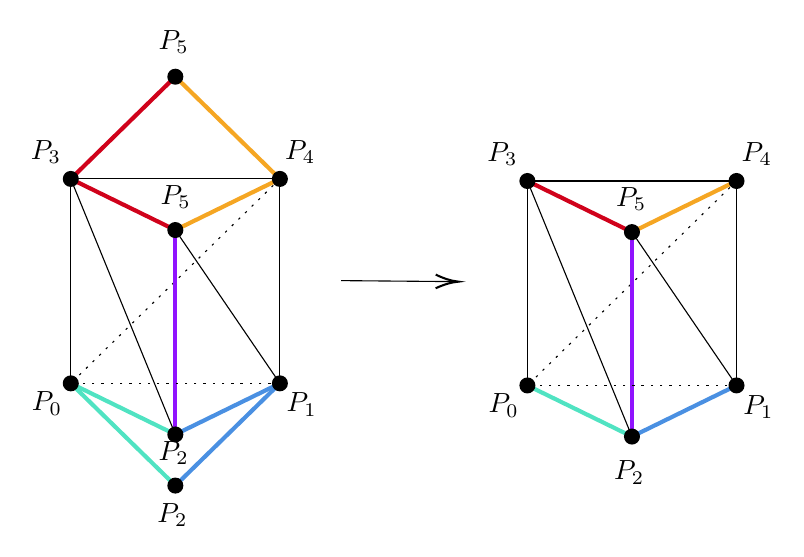
\begin{tikzpicture}[x=0.75pt,y=0.75pt,yscale=-1,xscale=1]
        %uncomment if require: \path (0,735); %set diagram left start at 0, and has height of 735

        %Straight Lines [id:da014002172140736846] 
        \draw  [dash pattern={on 0.84pt off 2.51pt}]  (159,90.5) -- (58.25,189) ;
        %Straight Lines [id:da36724333651798924] 
        \draw [color={rgb, 255:red, 208; green, 2; blue, 27 }  ,draw opacity=1 ][line width=1.5]    (58.25,90.5) -- (108.63,115.13) ;
        %Straight Lines [id:da6165387060737599] 
        \draw [color={rgb, 255:red, 245; green, 166; blue, 35 }  ,draw opacity=1 ][line width=1.5]    (108.63,115.13) -- (159,90.5) ;
        %Straight Lines [id:da9543420654226447] 
        \draw [color={rgb, 255:red, 144; green, 19; blue, 254 }  ,draw opacity=1 ][line width=1.5]    (108.63,115.13) -- (108.63,213.63) ;
        %Straight Lines [id:da6612348464423401] 
        \draw [color={rgb, 255:red, 80; green, 227; blue, 194 }  ,draw opacity=1 ][line width=1.5]    (58.25,189) -- (108.63,213.63) ;
        %Straight Lines [id:da6074920149015968] 
        \draw [color={rgb, 255:red, 74; green, 144; blue, 226 }  ,draw opacity=1 ][line width=1.5]    (108.63,213.63) -- (159,189) ;
        %Straight Lines [id:da660277789052643] 
        \draw    (58.25,90.5) -- (58.25,189) ;
        %Straight Lines [id:da7353537111209147] 
        \draw    (159,90.5) -- (159,189) ;
        %Straight Lines [id:da26795450144902255] 
        \draw  [dash pattern={on 0.84pt off 2.51pt}]  (159,189) -- (58.25,189) ;
        %Straight Lines [id:da7524844156160424] 
        \draw    (58.25,90.5) -- (108.63,213.63) ;
        %Straight Lines [id:da5937417946091332] 
        \draw    (108.63,115.13) -- (159,189) ;
        %Straight Lines [id:da19564047836219722] 
        \draw    (58.25,90.5) -- (159,90.5) ;
        %Straight Lines [id:da4613039622053816] 
        \draw [color={rgb, 255:red, 208; green, 2; blue, 27 }  ,draw opacity=1 ][line width=1.5]    (108.63,41.25) -- (58.25,90.5) ;
        %Straight Lines [id:da45611083442346856] 
        \draw [color={rgb, 255:red, 245; green, 166; blue, 35 }  ,draw opacity=1 ][line width=1.5]    (108.63,41.25) -- (159,90.5) ;
        %Straight Lines [id:da1161502977992599] 
        \draw [color={rgb, 255:red, 74; green, 144; blue, 226 }  ,draw opacity=1 ][line width=1.5]    (159,189) -- (108.63,238.25) ;
        %Straight Lines [id:da322811512194098] 
        \draw [color={rgb, 255:red, 80; green, 227; blue, 194 }  ,draw opacity=1 ][line width=1.5]    (58.25,189) -- (108.63,238.25) ;
        %Straight Lines [id:da7011452735974706] 
        \draw  [dash pattern={on 0.84pt off 2.51pt}]  (379,91.5) -- (278.25,190) ;
        %Straight Lines [id:da8171812351333771] 
        \draw [color={rgb, 255:red, 208; green, 2; blue, 27 }  ,draw opacity=1 ][line width=1.5]    (278.25,91.5) -- (328.63,116.13) ;
        %Straight Lines [id:da8791505710045846] 
        \draw [color={rgb, 255:red, 245; green, 166; blue, 35 }  ,draw opacity=1 ][line width=1.5]    (328.63,116.13) -- (379,91.5) ;
        %Straight Lines [id:da3168510651448171] 
        \draw [color={rgb, 255:red, 144; green, 19; blue, 254 }  ,draw opacity=1 ][line width=1.5]    (328.63,116.13) -- (328.63,214.63) ;
        %Straight Lines [id:da8344709154091496] 
        \draw [color={rgb, 255:red, 80; green, 227; blue, 194 }  ,draw opacity=1 ][line width=1.5]    (278.25,190) -- (328.63,214.63) ;
        %Straight Lines [id:da29229435991382413] 
        \draw [color={rgb, 255:red, 74; green, 144; blue, 226 }  ,draw opacity=1 ][line width=1.5]    (328.63,214.63) -- (379,190) ;
        %Straight Lines [id:da16018613721386665] 
        \draw    (278.25,91.5) -- (278.25,190) ;
        %Straight Lines [id:da8913334049218811] 
        \draw    (379,91.5) -- (379,190) ;
        %Straight Lines [id:da0018149378466838506] 
        \draw  [dash pattern={on 0.84pt off 2.51pt}]  (379,190) -- (278.25,190) ;
        %Straight Lines [id:da12776884666092192] 
        \draw    (278.25,91.5) -- (328.63,214.63) ;
        %Straight Lines [id:da15330791845306946] 
        \draw    (328.63,116.13) -- (379,190) ;
        %Straight Lines [id:da847752436318927] 
        \draw    (278.25,91.5) -- (379,91.5) ;
        %Straight Lines [id:da3273682931351978] 
        \draw    (188.5,139.5) -- (243,139.98) ;
        \draw [shift={(245,140)}, rotate = 180.51] [color={rgb, 255:red, 0; green, 0; blue, 0 }  ][line width=0.75]    (10.93,-3.29) .. controls (6.95,-1.4) and (3.31,-0.3) .. (0,0) .. controls (3.31,0.3) and (6.95,1.4) .. (10.93,3.29)   ;
        %Shape: Boxed Line [id:dp004492795298760566] 
        \draw    (159,90.5) ;
        \draw [shift={(159,90.5)}, rotate = 0] [color={rgb, 255:red, 0; green, 0; blue, 0 }  ][fill={rgb, 255:red, 0; green, 0; blue, 0 }  ][line width=0.75]      (0, 0) circle [x radius= 3.35, y radius= 3.35]   ;
        %Shape: Boxed Line [id:dp7326689861959503] 
        \draw    (278.25,190) ;
        \draw [shift={(278.25,190)}, rotate = 0] [color={rgb, 255:red, 0; green, 0; blue, 0 }  ][fill={rgb, 255:red, 0; green, 0; blue, 0 }  ][line width=0.75]      (0, 0) circle [x radius= 3.35, y radius= 3.35]   ;
        %Shape: Boxed Line [id:dp979902841378441] 
        \draw    (159,189) ;
        \draw [shift={(159,189)}, rotate = 0] [color={rgb, 255:red, 0; green, 0; blue, 0 }  ][fill={rgb, 255:red, 0; green, 0; blue, 0 }  ][line width=0.75]      (0, 0) circle [x radius= 3.35, y radius= 3.35]   ;
        %Shape: Boxed Line [id:dp13247643053070557] 
        \draw    (58.25,189) ;
        \draw [shift={(58.25,189)}, rotate = 0] [color={rgb, 255:red, 0; green, 0; blue, 0 }  ][fill={rgb, 255:red, 0; green, 0; blue, 0 }  ][line width=0.75]      (0, 0) circle [x radius= 3.35, y radius= 3.35]   ;
        %Shape: Boxed Line [id:dp6114259232645403] 
        \draw    (108.63,213.63) ;
        \draw [shift={(108.63,213.63)}, rotate = 0] [color={rgb, 255:red, 0; green, 0; blue, 0 }  ][fill={rgb, 255:red, 0; green, 0; blue, 0 }  ][line width=0.75]      (0, 0) circle [x radius= 3.35, y radius= 3.35]   ;
        %Shape: Boxed Line [id:dp11660761051574187] 
        \draw    (108.63,238.25) ;
        \draw [shift={(108.63,238.25)}, rotate = 0] [color={rgb, 255:red, 0; green, 0; blue, 0 }  ][fill={rgb, 255:red, 0; green, 0; blue, 0 }  ][line width=0.75]      (0, 0) circle [x radius= 3.35, y radius= 3.35]   ;
        %Shape: Boxed Line [id:dp3519212061308352] 
        \draw    (58.25,90.5) ;
        \draw [shift={(58.25,90.5)}, rotate = 0] [color={rgb, 255:red, 0; green, 0; blue, 0 }  ][fill={rgb, 255:red, 0; green, 0; blue, 0 }  ][line width=0.75]      (0, 0) circle [x radius= 3.35, y radius= 3.35]   ;
        %Shape: Boxed Line [id:dp956196782482418] 
        \draw    (108.63,115.13) ;
        \draw [shift={(108.63,115.13)}, rotate = 0] [color={rgb, 255:red, 0; green, 0; blue, 0 }  ][fill={rgb, 255:red, 0; green, 0; blue, 0 }  ][line width=0.75]      (0, 0) circle [x radius= 3.35, y radius= 3.35]   ;
        %Shape: Boxed Line [id:dp853558078166464] 
        \draw    (108.63,41.25) ;
        \draw [shift={(108.63,41.25)}, rotate = 0] [color={rgb, 255:red, 0; green, 0; blue, 0 }  ][fill={rgb, 255:red, 0; green, 0; blue, 0 }  ][line width=0.75]      (0, 0) circle [x radius= 3.35, y radius= 3.35]   ;
        %Shape: Boxed Line [id:dp5847784440436201] 
        \draw    (328.63,214.63) ;
        \draw [shift={(328.63,214.63)}, rotate = 0] [color={rgb, 255:red, 0; green, 0; blue, 0 }  ][fill={rgb, 255:red, 0; green, 0; blue, 0 }  ][line width=0.75]      (0, 0) circle [x radius= 3.35, y radius= 3.35]   ;
        %Shape: Boxed Line [id:dp47989309079086895] 
        \draw    (379,190) ;
        \draw [shift={(379,190)}, rotate = 0] [color={rgb, 255:red, 0; green, 0; blue, 0 }  ][fill={rgb, 255:red, 0; green, 0; blue, 0 }  ][line width=0.75]      (0, 0) circle [x radius= 3.35, y radius= 3.35]   ;
        %Shape: Boxed Line [id:dp3850330107391422] 
        \draw    (328.63,116.13) ;
        \draw [shift={(328.63,116.13)}, rotate = 0] [color={rgb, 255:red, 0; green, 0; blue, 0 }  ][fill={rgb, 255:red, 0; green, 0; blue, 0 }  ][line width=0.75]      (0, 0) circle [x radius= 3.35, y radius= 3.35]   ;
        %Shape: Boxed Line [id:dp02702522685468267] 
        \draw    (278.25,91.5) ;
        \draw [shift={(278.25,91.5)}, rotate = 0] [color={rgb, 255:red, 0; green, 0; blue, 0 }  ][fill={rgb, 255:red, 0; green, 0; blue, 0 }  ][line width=0.75]      (0, 0) circle [x radius= 3.35, y radius= 3.35]   ;
        %Shape: Boxed Line [id:dp3872013277202486] 
        \draw    (379,91.5) ;
        \draw [shift={(379,91.5)}, rotate = 0] [color={rgb, 255:red, 0; green, 0; blue, 0 }  ][fill={rgb, 255:red, 0; green, 0; blue, 0 }  ][line width=0.75]      (0, 0) circle [x radius= 3.35, y radius= 3.35]   ;

        % Text Node
        \draw (37.75,70.9) node [anchor=north west][inner sep=0.75pt]    {$P_{3}$};
        % Text Node
        \draw (38.25,191.9) node [anchor=north west][inner sep=0.75pt]    {$P_{0}$};
        % Text Node
        \draw (161,192.4) node [anchor=north west][inner sep=0.75pt]    {$P_{1}$};
        % Text Node
        \draw (160.25,70.9) node [anchor=north west][inner sep=0.75pt]    {$P_{4}$};
        % Text Node
        \draw (98.75,245.65) node [anchor=north west][inner sep=0.75pt]    {$P_{2}$};
        % Text Node
        \draw (99.25,17.9) node [anchor=north west][inner sep=0.75pt]    {$P_{5}$};
        % Text Node
        \draw (257.75,71.9) node [anchor=north west][inner sep=0.75pt]    {$P_{3}$};
        % Text Node
        \draw (258.25,192.9) node [anchor=north west][inner sep=0.75pt]    {$P_{0}$};
        % Text Node
        \draw (381,193.4) node [anchor=north west][inner sep=0.75pt]    {$P_{1}$};
        % Text Node
        \draw (380.25,71.9) node [anchor=north west][inner sep=0.75pt]    {$P_{4}$};
        % Text Node
        \draw (318.75,225.15) node [anchor=north west][inner sep=0.75pt]    {$P_{2}$};
        % Text Node
        \draw (319.75,93.4) node [anchor=north west][inner sep=0.75pt]    {$P_{5}$};
        % Text Node
        \draw (100.25,92.4) node [anchor=north west][inner sep=0.75pt]    {$P_{5}$};
        % Text Node
        \draw (99.25,215.65) node [anchor=north west][inner sep=0.75pt]    {$P_{2}$};


    \end{tikzpicture}

\end{center}
$S$ è isomorfo al vertex scheme di un complesso simpliciale in $\R^3$
\part{Omologia simpliciale}
\chapter{Omologia simpliciale}
\section{Gruppi di omologia simpliciale}
\begin{definition}[Gruppo delle p-catene]
    Sia $K$ un complesso simpliciale (geometrico o astratto), chiamiamo gruppo delle p-catene di $K$ il gruppo libero generato dai p-simplessi di $K$, ossia l'insieme
    \[
        C_p(K):=\setst{c:\{\text{p-simplessi di }K\}\ra\Z}{c^{-1}(\Z\setminus\{0\})\text{ ha cardinalità finita}}
    \]
    con l'operazione somma
    \[
        +:C_p(K)\times C_p(K)\ra C_p(K)
    \]
    \[
        (C+C')(\sigma)=C(\sigma)+ C'(\sigma)\quad \forall\sigma\text{ p-simplesso}
    \]
\end{definition}
\paragraph{N.B.} Per convenzione si ha
\[
    C_p(K)=\{0\}
\]
per $p>dim K$ oppure $p<0$
\paragraph{Osservazioni}
\begin{itemize}
    \item Posso consierare la stessa costruzione anche rispetto ad altri gruppi, ossia
          \[
              C_p(K):=\setst{c:\{\text{p-simplessi di }K\}\ra G}{c^{-1}(G\setminus\{0_G\})\text{ ha cardinalità finita}}
          \]
          casi interessanti sono $C_p(K,\Z_n)$
    \item Una base di $C_p(K)$ è formato dalle funzioni caratteristiche dei simplessi
          \[
              \forall\sigma\text{ p-simplesso},\quad C_\sigma(\tau)=\left\{\begin{array}{ll}
                  1 & \tau=\sigma    \\
                  0 & \tau\neq\sigma
              \end{array}\right.
          \]
          D'ora in poi, $\sigma$ indicherè il simplesso o la funzione caratteristica associata $C_\sigma$
\end{itemize}
\paragraph{Domanda} Che significato ha l'elemento opposto nel gruppo delle p-catene? Partiamo dall'elemento opposto degli elementi della base
\pagebreak
\paragraph{p=1}
\begin{center}
    \tikzset{every picture/.style={line width=0.75pt}}
    \begin{tikzpicture}[x=0.75pt,y=0.75pt,yscale=-1,xscale=1]
        \draw    (235,122) -- (307,50) ;
        \draw [shift={(307,50)}, rotate = 315] [color={rgb, 255:red, 0; green, 0; blue, 0 }  ][fill={rgb, 255:red, 0; green, 0; blue, 0 }  ][line width=0.75]      (0, 0) circle [x radius= 3.35, y radius= 3.35]   ;
        \draw [shift={(235,122)}, rotate = 315] [color={rgb, 255:red, 0; green, 0; blue, 0 }  ][fill={rgb, 255:red, 0; green, 0; blue, 0 }  ][line width=0.75]      (0, 0) circle [x radius= 3.35, y radius= 3.35]   ;
        \draw    (307,50) -- (383,99) ;
        \draw [shift={(383,99)}, rotate = 32.81] [color={rgb, 255:red, 0; green, 0; blue, 0 }  ][fill={rgb, 255:red, 0; green, 0; blue, 0 }  ][line width=0.75]      (0, 0) circle [x radius= 3.35, y radius= 3.35]   ;
        \draw (214,127.4) node [anchor=north west][inner sep=0.75pt]    {$P_{0}$};
        \draw (307,24.4) node [anchor=north west][inner sep=0.75pt]    {$P_{1}$};
        \draw (385,102.4) node [anchor=north west][inner sep=0.75pt]    {$P_{2}$};
    \end{tikzpicture}
\end{center}
Consideriamo il simplesso $\sigma=[P_0,P_1]$, otteniamo
\[
    \sigma_{[P_0,P_1]}([P_0,P_1])=1
\]
\[
    \sigma_{[P_1,P_2]}([P_0,P_1])=0
\]
cosa vuol dire $-\sigma_{[P_0,P_1]}$? Idea intuitiva: cambiamo il verso di percorrenza!\\
\paragraph{p=2}
\begin{center}


    \tikzset{every picture/.style={line width=0.75pt}} %set default line width to 0.75pt        

    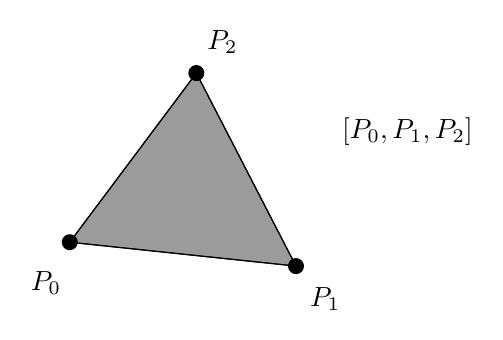
\begin{tikzpicture}[x=0.75pt,y=0.75pt,yscale=-1,xscale=1]
        %uncomment if require: \path (0,433); %set diagram left start at 0, and has height of 433

        %Shape: Polygon [id:ds36999198055717075] 
        \draw  [fill={rgb, 255:red, 155; green, 155; blue, 155 }  ,fill opacity=1 ] (161,27.5) -- (209,120.5) -- (209,120.5) -- (100,109) -- (100,109) -- cycle ;
        %Straight Lines [id:da1075961216776884] 
        \draw    (100,109) -- (161,27.5) ;
        \draw [shift={(161,27.5)}, rotate = 306.81] [color={rgb, 255:red, 0; green, 0; blue, 0 }  ][fill={rgb, 255:red, 0; green, 0; blue, 0 }  ][line width=0.75]      (0, 0) circle [x radius= 3.35, y radius= 3.35]   ;
        \draw [shift={(100,109)}, rotate = 306.81] [color={rgb, 255:red, 0; green, 0; blue, 0 }  ][fill={rgb, 255:red, 0; green, 0; blue, 0 }  ][line width=0.75]      (0, 0) circle [x radius= 3.35, y radius= 3.35]   ;
        %Straight Lines [id:da9479310379677153] 
        \draw    (100,109) -- (209,120.5) ;
        %Straight Lines [id:da47216061579231305] 
        \draw    (161,27.5) -- (209,120.5) ;
        \draw [shift={(209,120.5)}, rotate = 62.7] [color={rgb, 255:red, 0; green, 0; blue, 0 }  ][fill={rgb, 255:red, 0; green, 0; blue, 0 }  ][line width=0.75]      (0, 0) circle [x radius= 3.35, y radius= 3.35]   ;

        % Text Node
        \draw (80,121.9) node [anchor=north west][inner sep=0.75pt]    {$P_{0}$};
        % Text Node
        \draw (214.5,129.4) node [anchor=north west][inner sep=0.75pt]    {$P_{1}$};
        % Text Node
        \draw (165,5.9) node [anchor=north west][inner sep=0.75pt]    {$P_{2}$};
        % Text Node
        \draw (230,47.9) node [anchor=north west][inner sep=0.75pt]    {$[ P_{0} ,P_{1} ,P_{2}]$};


    \end{tikzpicture}

\end{center}
Cosa significa $-\sigma_{[P_0,P_1,P_2]}$? Nel nostro esempio, $[P_0,P_1,P_2]$ corrisponde all'esplorare i vertici in senso antiorario, quindi $-[P_0,P_1,P_2]$ potrebbe significare esplorare i vertici in senso orario
\begin{center}


    \tikzset{every picture/.style={line width=0.75pt}} %set default line width to 0.75pt        

    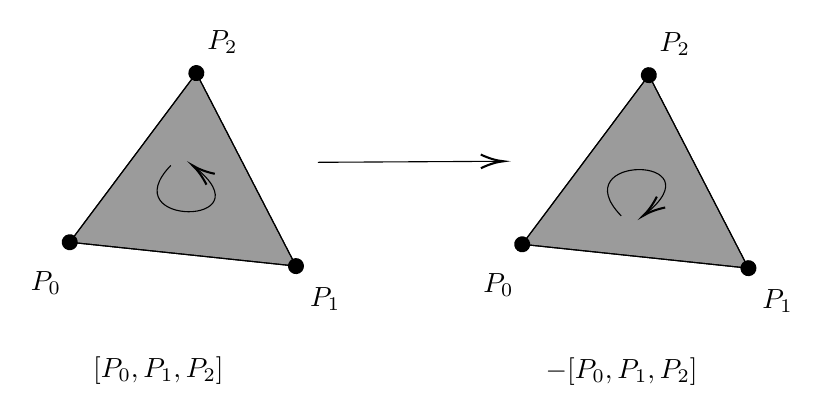
\begin{tikzpicture}[x=0.75pt,y=0.75pt,yscale=-1,xscale=1]
        %uncomment if require: \path (0,433); %set diagram left start at 0, and has height of 433

        %Shape: Polygon [id:ds36999198055717075] 
        \draw  [fill={rgb, 255:red, 155; green, 155; blue, 155 }  ,fill opacity=1 ] (161,27.5) -- (209,120.5) -- (209,120.5) -- (100,109) -- (100,109) -- cycle ;
        %Straight Lines [id:da1075961216776884] 
        \draw    (100,109) -- (161,27.5) ;
        \draw [shift={(161,27.5)}, rotate = 306.81] [color={rgb, 255:red, 0; green, 0; blue, 0 }  ][fill={rgb, 255:red, 0; green, 0; blue, 0 }  ][line width=0.75]      (0, 0) circle [x radius= 3.35, y radius= 3.35]   ;
        \draw [shift={(100,109)}, rotate = 306.81] [color={rgb, 255:red, 0; green, 0; blue, 0 }  ][fill={rgb, 255:red, 0; green, 0; blue, 0 }  ][line width=0.75]      (0, 0) circle [x radius= 3.35, y radius= 3.35]   ;
        %Straight Lines [id:da9479310379677153] 
        \draw    (100,109) -- (209,120.5) ;
        %Straight Lines [id:da47216061579231305] 
        \draw    (161,27.5) -- (209,120.5) ;
        \draw [shift={(209,120.5)}, rotate = 62.7] [color={rgb, 255:red, 0; green, 0; blue, 0 }  ][fill={rgb, 255:red, 0; green, 0; blue, 0 }  ][line width=0.75]      (0, 0) circle [x radius= 3.35, y radius= 3.35]   ;
        %Shape: Polygon [id:ds7233091919690151] 
        \draw  [fill={rgb, 255:red, 155; green, 155; blue, 155 }  ,fill opacity=1 ] (379,28.5) -- (427,121.5) -- (427,121.5) -- (318,110) -- (318,110) -- cycle ;
        %Straight Lines [id:da467473520709776] 
        \draw    (318,110) -- (379,28.5) ;
        \draw [shift={(379,28.5)}, rotate = 306.81] [color={rgb, 255:red, 0; green, 0; blue, 0 }  ][fill={rgb, 255:red, 0; green, 0; blue, 0 }  ][line width=0.75]      (0, 0) circle [x radius= 3.35, y radius= 3.35]   ;
        \draw [shift={(318,110)}, rotate = 306.81] [color={rgb, 255:red, 0; green, 0; blue, 0 }  ][fill={rgb, 255:red, 0; green, 0; blue, 0 }  ][line width=0.75]      (0, 0) circle [x radius= 3.35, y radius= 3.35]   ;
        %Straight Lines [id:da8439250097390936] 
        \draw    (318,110) -- (427,121.5) ;
        %Straight Lines [id:da38059697243757573] 
        \draw    (379,28.5) -- (427,121.5) ;
        \draw [shift={(427,121.5)}, rotate = 62.7] [color={rgb, 255:red, 0; green, 0; blue, 0 }  ][fill={rgb, 255:red, 0; green, 0; blue, 0 }  ][line width=0.75]      (0, 0) circle [x radius= 3.35, y radius= 3.35]   ;
        %Shape: Boxed Bezier Curve [id:dp21432790645980138] 
        \draw    (365.7,96.31) .. controls (336.99,66.61) and (413.16,66.81) .. (377.33,95.44) ;
        \draw [shift={(376.2,96.31)}, rotate = 322.54] [color={rgb, 255:red, 0; green, 0; blue, 0 }  ][line width=0.75]    (10.93,-3.29) .. controls (6.95,-1.4) and (3.31,-0.3) .. (0,0) .. controls (3.31,0.3) and (6.95,1.4) .. (10.93,3.29)   ;
        %Shape: Boxed Bezier Curve [id:dp47408798381826833] 
        \draw    (148.7,72) .. controls (119.99,101.7) and (196.16,101.51) .. (160.33,72.88) ;
        \draw [shift={(159.2,72)}, rotate = 37.46] [color={rgb, 255:red, 0; green, 0; blue, 0 }  ][line width=0.75]    (10.93,-3.29) .. controls (6.95,-1.4) and (3.31,-0.3) .. (0,0) .. controls (3.31,0.3) and (6.95,1.4) .. (10.93,3.29)   ;
        %Straight Lines [id:da09276962834026659] 
        \draw    (219.5,70.5) -- (307,70.01) ;
        \draw [shift={(309,70)}, rotate = 179.68] [color={rgb, 255:red, 0; green, 0; blue, 0 }  ][line width=0.75]    (10.93,-3.29) .. controls (6.95,-1.4) and (3.31,-0.3) .. (0,0) .. controls (3.31,0.3) and (6.95,1.4) .. (10.93,3.29)   ;

        % Text Node
        \draw (80,121.9) node [anchor=north west][inner sep=0.75pt]    {$P_{0}$};
        % Text Node
        \draw (214.5,129.4) node [anchor=north west][inner sep=0.75pt]    {$P_{1}$};
        % Text Node
        \draw (165,5.9) node [anchor=north west][inner sep=0.75pt]    {$P_{2}$};
        % Text Node
        \draw (110,162.9) node [anchor=north west][inner sep=0.75pt]    {$[ P_{0} ,P_{1} ,P_{2}]$};
        % Text Node
        \draw (298,122.9) node [anchor=north west][inner sep=0.75pt]    {$P_{0}$};
        % Text Node
        \draw (432.5,130.4) node [anchor=north west][inner sep=0.75pt]    {$P_{1}$};
        % Text Node
        \draw (383,6.9) node [anchor=north west][inner sep=0.75pt]    {$P_{2}$};
        % Text Node
        \draw (328,163.4) node [anchor=north west][inner sep=0.75pt]    {$-[ P_{0} ,P_{1} ,P_{2}]$};


    \end{tikzpicture}

\end{center}
Ossia intendiamo
\[
    -[P_0,P_1,P_2]=[P_0,P_2,P_1]
\]
\paragraph{In generale}
In generale è difficile estendere intuitivamente il concetto a p-simplessi di dimensione superiore (e nemmeno a 0-simplessi)
\begin{definition}[Ordinamenti equivalenti]
    Sia $\sigma$ un p-simplesso. Diciamo che due ordinamenti dei vertici di $\sigma$ sono equivalenti se differiscono per un numero pari di scambi (cioè per una permutazione pari).\\
    Le due classi di equivalenza si dicono ordinamenti di $\sigma$
\end{definition}
\begin{definition}[Simplesso orientato]
    Un simplesso orientato è un simplesso con una delle sue orientazioni fissata
\end{definition}
\paragraph{Esempi}
\paragraph{p=0} $\{0\}$ ho una sola orientazione
\paragraph{p=1} $[P_0,P_1]$. Ho due orientamenti possibili, che differiscono per uno scambio
\begin{center}


    \tikzset{every picture/.style={line width=0.75pt}} %set default line width to 0.75pt        

    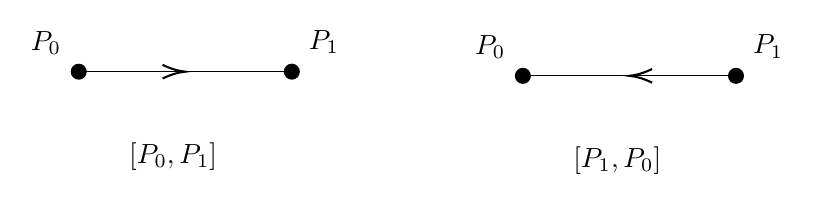
\begin{tikzpicture}[x=0.75pt,y=0.75pt,yscale=-1,xscale=1]
        %uncomment if require: \path (0,300); %set diagram left start at 0, and has height of 300

        %Straight Lines [id:da8093053903679137] 
        \draw    (99,109.33) -- (201.67,109.33) ;
        \draw [shift={(201.67,109.33)}, rotate = 0] [color={rgb, 255:red, 0; green, 0; blue, 0 }  ][fill={rgb, 255:red, 0; green, 0; blue, 0 }  ][line width=0.75]      (0, 0) circle [x radius= 3.35, y radius= 3.35]   ;
        \draw [shift={(99,109.33)}, rotate = 0] [color={rgb, 255:red, 0; green, 0; blue, 0 }  ][fill={rgb, 255:red, 0; green, 0; blue, 0 }  ][line width=0.75]      (0, 0) circle [x radius= 3.35, y radius= 3.35]   ;
        %Straight Lines [id:da5741629828716988] 
        \draw    (99,109.33) -- (148.33,109.33) ;
        \draw [shift={(150.33,109.33)}, rotate = 180] [color={rgb, 255:red, 0; green, 0; blue, 0 }  ][line width=0.75]    (10.93,-3.29) .. controls (6.95,-1.4) and (3.31,-0.3) .. (0,0) .. controls (3.31,0.3) and (6.95,1.4) .. (10.93,3.29)   ;
        %Straight Lines [id:da8184939293192373] 
        \draw    (313,111.33) -- (415.67,111.33) ;
        \draw [shift={(415.67,111.33)}, rotate = 0] [color={rgb, 255:red, 0; green, 0; blue, 0 }  ][fill={rgb, 255:red, 0; green, 0; blue, 0 }  ][line width=0.75]      (0, 0) circle [x radius= 3.35, y radius= 3.35]   ;
        \draw [shift={(313,111.33)}, rotate = 0] [color={rgb, 255:red, 0; green, 0; blue, 0 }  ][fill={rgb, 255:red, 0; green, 0; blue, 0 }  ][line width=0.75]      (0, 0) circle [x radius= 3.35, y radius= 3.35]   ;
        %Straight Lines [id:da28007999881288304] 
        \draw    (415.67,111.33) -- (366.33,111.33) ;
        \draw [shift={(364.33,111.33)}, rotate = 360] [color={rgb, 255:red, 0; green, 0; blue, 0 }  ][line width=0.75]    (10.93,-3.29) .. controls (6.95,-1.4) and (3.31,-0.3) .. (0,0) .. controls (3.31,0.3) and (6.95,1.4) .. (10.93,3.29)   ;

        % Text Node
        \draw (74.67,88.73) node [anchor=north west][inner sep=0.75pt]    {$P_{0}$};
        % Text Node
        \draw (208.67,88.4) node [anchor=north west][inner sep=0.75pt]    {$P_{1}$};
        % Text Node
        \draw (122,142.4) node [anchor=north west][inner sep=0.75pt]    {$[ P_{0} ,P_{1}]$};
        % Text Node
        \draw (288.67,90.73) node [anchor=north west][inner sep=0.75pt]    {$P_{0}$};
        % Text Node
        \draw (422.67,90.4) node [anchor=north west][inner sep=0.75pt]    {$P_{1}$};
        % Text Node
        \draw (336,144.4) node [anchor=north west][inner sep=0.75pt]    {$[ P_{1} ,P_{0}]$};


    \end{tikzpicture}

\end{center}
\paragraph{p=2} Possiamo dividere gli ordinamenti in due classi di equivalenza, corrispondenti ad una visita dei vertici in senso orario o antiorario
\begin{center}


    \tikzset{every picture/.style={line width=0.75pt}} %set default line width to 0.75pt        

    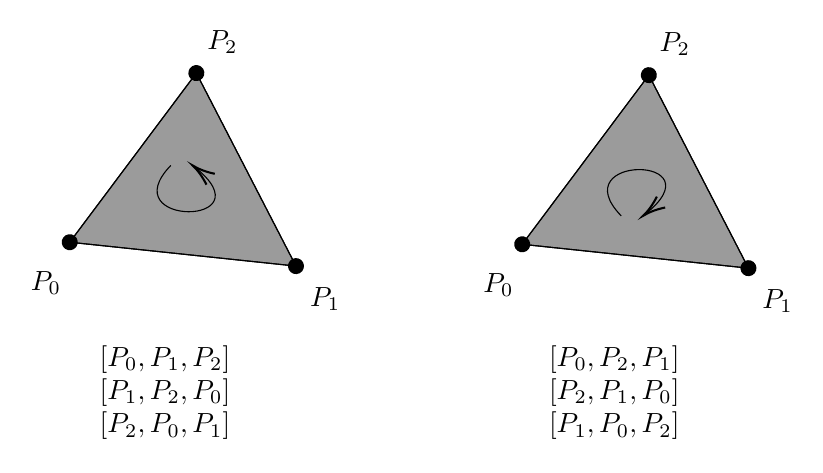
\begin{tikzpicture}[x=0.75pt,y=0.75pt,yscale=-1,xscale=1]
        %uncomment if require: \path (0,433); %set diagram left start at 0, and has height of 433

        %Shape: Polygon [id:ds36999198055717075] 
        \draw  [fill={rgb, 255:red, 155; green, 155; blue, 155 }  ,fill opacity=1 ] (161,27.5) -- (209,120.5) -- (209,120.5) -- (100,109) -- (100,109) -- cycle ;
        %Straight Lines [id:da1075961216776884] 
        \draw    (100,109) -- (161,27.5) ;
        \draw [shift={(161,27.5)}, rotate = 306.81] [color={rgb, 255:red, 0; green, 0; blue, 0 }  ][fill={rgb, 255:red, 0; green, 0; blue, 0 }  ][line width=0.75]      (0, 0) circle [x radius= 3.35, y radius= 3.35]   ;
        \draw [shift={(100,109)}, rotate = 306.81] [color={rgb, 255:red, 0; green, 0; blue, 0 }  ][fill={rgb, 255:red, 0; green, 0; blue, 0 }  ][line width=0.75]      (0, 0) circle [x radius= 3.35, y radius= 3.35]   ;
        %Straight Lines [id:da9479310379677153] 
        \draw    (100,109) -- (209,120.5) ;
        %Straight Lines [id:da47216061579231305] 
        \draw    (161,27.5) -- (209,120.5) ;
        \draw [shift={(209,120.5)}, rotate = 62.7] [color={rgb, 255:red, 0; green, 0; blue, 0 }  ][fill={rgb, 255:red, 0; green, 0; blue, 0 }  ][line width=0.75]      (0, 0) circle [x radius= 3.35, y radius= 3.35]   ;
        %Shape: Polygon [id:ds7233091919690151] 
        \draw  [fill={rgb, 255:red, 155; green, 155; blue, 155 }  ,fill opacity=1 ] (379,28.5) -- (427,121.5) -- (427,121.5) -- (318,110) -- (318,110) -- cycle ;
        %Straight Lines [id:da467473520709776] 
        \draw    (318,110) -- (379,28.5) ;
        \draw [shift={(379,28.5)}, rotate = 306.81] [color={rgb, 255:red, 0; green, 0; blue, 0 }  ][fill={rgb, 255:red, 0; green, 0; blue, 0 }  ][line width=0.75]      (0, 0) circle [x radius= 3.35, y radius= 3.35]   ;
        \draw [shift={(318,110)}, rotate = 306.81] [color={rgb, 255:red, 0; green, 0; blue, 0 }  ][fill={rgb, 255:red, 0; green, 0; blue, 0 }  ][line width=0.75]      (0, 0) circle [x radius= 3.35, y radius= 3.35]   ;
        %Straight Lines [id:da8439250097390936] 
        \draw    (318,110) -- (427,121.5) ;
        %Straight Lines [id:da38059697243757573] 
        \draw    (379,28.5) -- (427,121.5) ;
        \draw [shift={(427,121.5)}, rotate = 62.7] [color={rgb, 255:red, 0; green, 0; blue, 0 }  ][fill={rgb, 255:red, 0; green, 0; blue, 0 }  ][line width=0.75]      (0, 0) circle [x radius= 3.35, y radius= 3.35]   ;
        %Shape: Boxed Bezier Curve [id:dp21432790645980138] 
        \draw    (365.7,96.31) .. controls (336.99,66.61) and (413.16,66.81) .. (377.33,95.44) ;
        \draw [shift={(376.2,96.31)}, rotate = 322.54] [color={rgb, 255:red, 0; green, 0; blue, 0 }  ][line width=0.75]    (10.93,-3.29) .. controls (6.95,-1.4) and (3.31,-0.3) .. (0,0) .. controls (3.31,0.3) and (6.95,1.4) .. (10.93,3.29)   ;
        %Shape: Boxed Bezier Curve [id:dp47408798381826833] 
        \draw    (148.7,72) .. controls (119.99,101.7) and (196.16,101.51) .. (160.33,72.88) ;
        \draw [shift={(159.2,72)}, rotate = 37.46] [color={rgb, 255:red, 0; green, 0; blue, 0 }  ][line width=0.75]    (10.93,-3.29) .. controls (6.95,-1.4) and (3.31,-0.3) .. (0,0) .. controls (3.31,0.3) and (6.95,1.4) .. (10.93,3.29)   ;

        % Text Node
        \draw (80,121.9) node [anchor=north west][inner sep=0.75pt]    {$P_{0}$};
        % Text Node
        \draw (214.5,129.4) node [anchor=north west][inner sep=0.75pt]    {$P_{1}$};
        % Text Node
        \draw (165,5.9) node [anchor=north west][inner sep=0.75pt]    {$P_{2}$};
        % Text Node
        \draw (298,122.9) node [anchor=north west][inner sep=0.75pt]    {$P_{0}$};
        % Text Node
        \draw (432.5,130.4) node [anchor=north west][inner sep=0.75pt]    {$P_{1}$};
        % Text Node
        \draw (383,6.9) node [anchor=north west][inner sep=0.75pt]    {$P_{2}$};
        % Text Node
        \draw (106.5,156.4) node [anchor=north west][inner sep=0.75pt]    {$\begin{array}{ c }
                    {[} P_{0} ,P_{1} ,P_{2}{]} \\
                    {[} P_{1} ,P_{2} ,P_{0}{]} \\
                    {[} P_{2} ,P_{0} ,P_{1}{]}
                \end{array}$};
        % Text Node
        \draw (323,156.4) node [anchor=north west][inner sep=0.75pt]    {$\begin{array}{ c }
                    {[} P_{0} ,P_{2} ,P_{1}{]} \\
                    {[} P_{2} ,P_{1} ,P_{0}{]} \\
                    {[} P_{1} ,P_{0} ,P_{2}{]}
                \end{array}$};


    \end{tikzpicture}

\end{center}
Possiamo ora migliorare la nostra definizione di gruppo delle p-catene di un complesso simpliciale
\begin{definition}[Gruppo delle p-catene v2]
    Sia $K$ un complesso simpliciale (geometrico o astratto), con una orientazione fissata per ogni silesso, chiamiamo gruppo delle p-catene di $K$ il gruppo libero generato dai p-simplessi di $K$, ossia l'insieme
    \[
        C_p(K):=\setst{c:\{\text{p-simplessi di }K\}\ra\Z}{c^{-1}(\Z\setminus\{0\})\text{ ha cardinalità finita}}
    \]
    con l'operazione somma
    \[
        +:C_p(K)\times C_p(K)\ra C_p(K)
    \]
    \[
        (C+C')(\sigma)=C(\sigma)+ C'(\sigma)\quad \forall\sigma\text{ p-simplesso}
    \]
\end{definition}
\begin{definition}[P-esimo operatore di bordo]
    Sia $K$ un complesso simpliciale, definiamo p-esimo operatore di bordo l'omomorfismo di gruppi
    \[
        \partial_p:C_p(K)\ra C_{p-1}(K)
    \]
    definito come
    \[
        \sigma=[P_0,P_1,\dots,P_p]\longmapsto\sum_{i=0}^p(-1)^i[P_0,\dots,P_{i-1},\hat{P_i},P_{i+1},\dots,P_p]
    \]
    dove con $\hat{P_i}$ intendiamo che l'elemento $P_i$ viene rimosso dalla collezione di punti che generano il simplesso
\end{definition}
\paragraph{Osservazione}
\[
    C_p(K)=\{0\}\quad p<0\implies \partial_p=0\quad p\leq 0
\]
\paragraph{Esempio}
\paragraph{p=1}
Consideriamo il complesso simpliciale
\begin{center}


    \tikzset{every picture/.style={line width=0.75pt}} %set default line width to 0.75pt        

    \begin{tikzpicture}[x=0.75pt,y=0.75pt,yscale=-1,xscale=1]
        %uncomment if require: \path (0,300); %set diagram left start at 0, and has height of 300

        %Straight Lines [id:da48607700170924506] 
        \draw    (100,118) -- (175,54) ;
        \draw [shift={(175,54)}, rotate = 319.52] [color={rgb, 255:red, 0; green, 0; blue, 0 }  ][fill={rgb, 255:red, 0; green, 0; blue, 0 }  ][line width=0.75]      (0, 0) circle [x radius= 3.35, y radius= 3.35]   ;
        \draw [shift={(100,118)}, rotate = 319.52] [color={rgb, 255:red, 0; green, 0; blue, 0 }  ][fill={rgb, 255:red, 0; green, 0; blue, 0 }  ][line width=0.75]      (0, 0) circle [x radius= 3.35, y radius= 3.35]   ;
        %Straight Lines [id:da2654155053672578] 
        \draw    (175,54) -- (214.33,159.33) ;
        \draw [shift={(214.33,159.33)}, rotate = 69.52] [color={rgb, 255:red, 0; green, 0; blue, 0 }  ][fill={rgb, 255:red, 0; green, 0; blue, 0 }  ][line width=0.75]      (0, 0) circle [x radius= 3.35, y radius= 3.35]   ;
        %Straight Lines [id:da6708083702244267] 
        \draw    (100,118) -- (135.98,87.3) ;
        \draw [shift={(137.5,86)}, rotate = 139.52] [color={rgb, 255:red, 0; green, 0; blue, 0 }  ][line width=0.75]    (10.93,-3.29) .. controls (6.95,-1.4) and (3.31,-0.3) .. (0,0) .. controls (3.31,0.3) and (6.95,1.4) .. (10.93,3.29)   ;
        %Straight Lines [id:da4078219573961033] 
        \draw    (175,54) -- (193.97,104.79) ;
        \draw [shift={(194.67,106.67)}, rotate = 249.52] [color={rgb, 255:red, 0; green, 0; blue, 0 }  ][line width=0.75]    (10.93,-3.29) .. controls (6.95,-1.4) and (3.31,-0.3) .. (0,0) .. controls (3.31,0.3) and (6.95,1.4) .. (10.93,3.29)   ;

        % Text Node
        \draw (78,126.73) node [anchor=north west][inner sep=0.75pt]    {$P_{0}$};
        % Text Node
        \draw (174.67,31.07) node [anchor=north west][inner sep=0.75pt]    {$P_{1}$};
        % Text Node
        \draw (216.33,162.73) node [anchor=north west][inner sep=0.75pt]    {$P_{2}$};


    \end{tikzpicture}

\end{center}
\[
    \partial_1[P_0,P_1]=(-1)^0[P_1]+(-1)^1[P_0]=[P_1]-[P_0]
\]
\[
    \partial_1[P_1,P_2]=(-1)^0[P_2]+(-1)^1[P_1]=[P_2]-[P_1]
\]
\[
    \partial_1([P_1,P_2]+[P_1,P_2])=\partial_1[P_0,P_1]+\partial_1[P_1,P_2]=P_1-P_0+P_2-P_1=P_2-P_0
\]
\pagebreak
\paragraph{Osservazione} Posso rappresentare gli operatori di bordo come matrici.\\
Consideriamo il complesso simpliciale $K$
\[
    K=\{[P_0,P_1,P_2],[P_0,P_1],[P_1,P_2],[P_0,P_2],[P_1,P_3],[P_0],[P_1],[P_2],[P_3]\}
\]
\begin{center}


    \tikzset{every picture/.style={line width=0.75pt}} %set default line width to 0.75pt        

    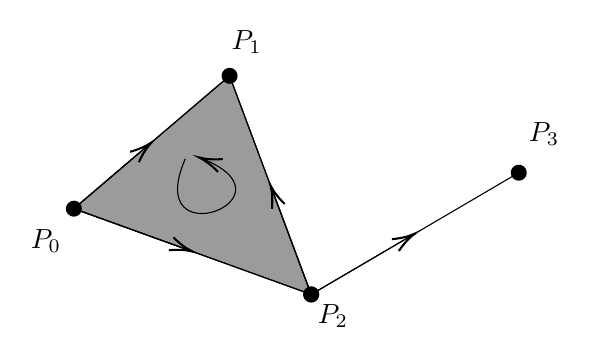
\begin{tikzpicture}[x=0.75pt,y=0.75pt,yscale=-1,xscale=1]
        %uncomment if require: \path (0,300); %set diagram left start at 0, and has height of 300

        %Shape: Polygon [id:ds28297359739544503] 
        \draw  [fill={rgb, 255:red, 155; green, 155; blue, 155 }  ,fill opacity=1 ] (175,54) -- (214.33,159.33) -- (100,118) -- (100,118) -- (175,54) -- cycle ;
        %Straight Lines [id:da48607700170924506] 
        \draw    (100,118) -- (175,54) ;
        \draw [shift={(175,54)}, rotate = 319.52] [color={rgb, 255:red, 0; green, 0; blue, 0 }  ][fill={rgb, 255:red, 0; green, 0; blue, 0 }  ][line width=0.75]      (0, 0) circle [x radius= 3.35, y radius= 3.35]   ;
        \draw [shift={(100,118)}, rotate = 319.52] [color={rgb, 255:red, 0; green, 0; blue, 0 }  ][fill={rgb, 255:red, 0; green, 0; blue, 0 }  ][line width=0.75]      (0, 0) circle [x radius= 3.35, y radius= 3.35]   ;
        %Straight Lines [id:da2654155053672578] 
        \draw    (175,54) -- (214.33,159.33) ;
        \draw [shift={(214.33,159.33)}, rotate = 69.52] [color={rgb, 255:red, 0; green, 0; blue, 0 }  ][fill={rgb, 255:red, 0; green, 0; blue, 0 }  ][line width=0.75]      (0, 0) circle [x radius= 3.35, y radius= 3.35]   ;
        %Straight Lines [id:da6708083702244267] 
        \draw    (100,118) -- (135.98,87.3) ;
        \draw [shift={(137.5,86)}, rotate = 139.52] [color={rgb, 255:red, 0; green, 0; blue, 0 }  ][line width=0.75]    (10.93,-3.29) .. controls (6.95,-1.4) and (3.31,-0.3) .. (0,0) .. controls (3.31,0.3) and (6.95,1.4) .. (10.93,3.29)   ;
        %Straight Lines [id:da4078219573961033] 
        \draw    (214.33,159.33) -- (195.37,108.54) ;
        \draw [shift={(194.67,106.67)}, rotate = 69.52] [color={rgb, 255:red, 0; green, 0; blue, 0 }  ][line width=0.75]    (10.93,-3.29) .. controls (6.95,-1.4) and (3.31,-0.3) .. (0,0) .. controls (3.31,0.3) and (6.95,1.4) .. (10.93,3.29)   ;
        %Straight Lines [id:da39756132351234275] 
        \draw    (100,118) -- (214.33,159.33) ;
        %Straight Lines [id:da7285879029160456] 
        \draw    (100,118) -- (155.29,137.99) ;
        \draw [shift={(157.17,138.67)}, rotate = 199.88] [color={rgb, 255:red, 0; green, 0; blue, 0 }  ][line width=0.75]    (10.93,-3.29) .. controls (6.95,-1.4) and (3.31,-0.3) .. (0,0) .. controls (3.31,0.3) and (6.95,1.4) .. (10.93,3.29)   ;
        %Straight Lines [id:da7484971508339138] 
        \draw    (314.33,100.67) -- (214.33,159.33) ;
        \draw [shift={(214.33,159.33)}, rotate = 149.6] [color={rgb, 255:red, 0; green, 0; blue, 0 }  ][fill={rgb, 255:red, 0; green, 0; blue, 0 }  ][line width=0.75]      (0, 0) circle [x radius= 3.35, y radius= 3.35]   ;
        \draw [shift={(314.33,100.67)}, rotate = 149.6] [color={rgb, 255:red, 0; green, 0; blue, 0 }  ][fill={rgb, 255:red, 0; green, 0; blue, 0 }  ][line width=0.75]      (0, 0) circle [x radius= 3.35, y radius= 3.35]   ;
        %Straight Lines [id:da5994508750727658] 
        \draw    (214.33,159.33) -- (262.61,131.01) ;
        \draw [shift={(264.33,130)}, rotate = 149.6] [color={rgb, 255:red, 0; green, 0; blue, 0 }  ][line width=0.75]    (10.93,-3.29) .. controls (6.95,-1.4) and (3.31,-0.3) .. (0,0) .. controls (3.31,0.3) and (6.95,1.4) .. (10.93,3.29)   ;
        %Curve Lines [id:da24647150418394692] 
        \draw    (153.67,94) .. controls (132.55,142.18) and (210.09,113.26) .. (161.83,93.92) ;
        \draw [shift={(160.33,93.33)}, rotate = 20.64] [color={rgb, 255:red, 0; green, 0; blue, 0 }  ][line width=0.75]    (10.93,-3.29) .. controls (6.95,-1.4) and (3.31,-0.3) .. (0,0) .. controls (3.31,0.3) and (6.95,1.4) .. (10.93,3.29)   ;

        % Text Node
        \draw (78,126.73) node [anchor=north west][inner sep=0.75pt]    {$P_{0}$};
        % Text Node
        \draw (174.67,31.07) node [anchor=north west][inner sep=0.75pt]    {$P_{1}$};
        % Text Node
        \draw (216.33,162.73) node [anchor=north west][inner sep=0.75pt]    {$P_{2}$};
        % Text Node
        \draw (318,75.07) node [anchor=north west][inner sep=0.75pt]    {$P_{3}$};


    \end{tikzpicture}

\end{center}
I gruppi delle p-catene risultano essere
\[
    C_p(K)=\{0\}\quad p<0\lor p>2
\]
\[
    C_0(K)=\gen{\{P_0,P_1,P_2,P_3\}}\simeq\Z^4
\]
\[
    C_1(K)=\gen{\{[P_0,P_1],[P_1,P_2],[P_0,P_2],[P_1,P_3]\}}\simeq\Z^4
\]
\[
    C_2(K)=\gen{[P_0,P_1,P_2]}\simeq\Z
\]
Gli operatori bordo risultano essere
\[
    \partial_p=0\quad p\leq 0\lor p>2
\]
\[
    \partial_2:C_2(K)\ra C_1(K)
\]
\[
    \partial_2[P_0,P_1,P_2]=(-1)^0[P_1,P_2]+(-1)^1[P_0,P_2]+(-1)^2[P_0,P_1]=
\]
\[
    =[P_0,P_1]+[P_1,P_2]-[P_0,P_2]
\]
posso rappresentrare l'opearatore tramite una matrice
\[
    \mathcal{M}_{3\times 1}(\Z)\ni\partial_2=\overset{[P_0,P_1,P_2]}{\left[
            \begin{array}{ll}
                1  \\
                1  \\
                -1 \\
                0
            \end{array}
            \right]}
    \begin{array}{ll}
        {[}P_0,P_1{]} \\
        {[}P_1,P_2{]} \\
        {[}P_0,P_2{]} \\
        {[}P_1,P_3{]}
    \end{array}
\]
\begin{center}


    \tikzset{every picture/.style={line width=0.75pt}} %set default line width to 0.75pt        

    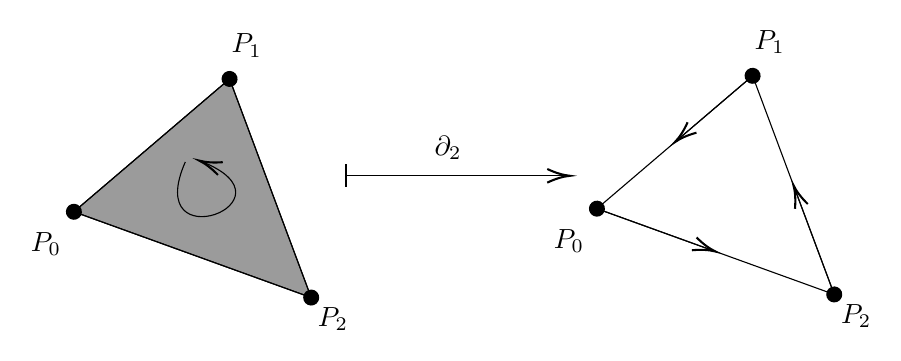
\begin{tikzpicture}[x=0.75pt,y=0.75pt,yscale=-1,xscale=1]
        %uncomment if require: \path (0,300); %set diagram left start at 0, and has height of 300

        %Shape: Polygon [id:ds28297359739544503] 
        \draw  [fill={rgb, 255:red, 155; green, 155; blue, 155 }  ,fill opacity=1 ] (175,54) -- (214.33,159.33) -- (100,118) -- (100,118) -- (175,54) -- cycle ;
        %Straight Lines [id:da48607700170924506] 
        \draw    (100,118) -- (175,54) ;
        \draw [shift={(175,54)}, rotate = 319.52] [color={rgb, 255:red, 0; green, 0; blue, 0 }  ][fill={rgb, 255:red, 0; green, 0; blue, 0 }  ][line width=0.75]      (0, 0) circle [x radius= 3.35, y radius= 3.35]   ;
        \draw [shift={(100,118)}, rotate = 319.52] [color={rgb, 255:red, 0; green, 0; blue, 0 }  ][fill={rgb, 255:red, 0; green, 0; blue, 0 }  ][line width=0.75]      (0, 0) circle [x radius= 3.35, y radius= 3.35]   ;
        %Straight Lines [id:da2654155053672578] 
        \draw    (175,54) -- (214.33,159.33) ;
        \draw [shift={(214.33,159.33)}, rotate = 69.52] [color={rgb, 255:red, 0; green, 0; blue, 0 }  ][fill={rgb, 255:red, 0; green, 0; blue, 0 }  ][line width=0.75]      (0, 0) circle [x radius= 3.35, y radius= 3.35]   ;
        %Straight Lines [id:da39756132351234275] 
        \draw    (100,118) -- (214.33,159.33) ;
        %Curve Lines [id:da24647150418394692] 
        \draw    (153.67,94) .. controls (132.55,142.18) and (210.09,113.26) .. (161.83,93.92) ;
        \draw [shift={(160.33,93.33)}, rotate = 20.64] [color={rgb, 255:red, 0; green, 0; blue, 0 }  ][line width=0.75]    (10.93,-3.29) .. controls (6.95,-1.4) and (3.31,-0.3) .. (0,0) .. controls (3.31,0.3) and (6.95,1.4) .. (10.93,3.29)   ;
        %Straight Lines [id:da12372196953986614] 
        \draw    (231,100.67) -- (337,100.67) ;
        \draw [shift={(339,100.67)}, rotate = 180] [color={rgb, 255:red, 0; green, 0; blue, 0 }  ][line width=0.75]    (10.93,-3.29) .. controls (6.95,-1.4) and (3.31,-0.3) .. (0,0) .. controls (3.31,0.3) and (6.95,1.4) .. (10.93,3.29)   ;
        \draw [shift={(231,100.67)}, rotate = 180] [color={rgb, 255:red, 0; green, 0; blue, 0 }  ][line width=0.75]    (0,5.59) -- (0,-5.59)   ;
        %Straight Lines [id:da6259440280694046] 
        \draw    (352,116.5) -- (427,52.5) ;
        \draw [shift={(427,52.5)}, rotate = 319.52] [color={rgb, 255:red, 0; green, 0; blue, 0 }  ][fill={rgb, 255:red, 0; green, 0; blue, 0 }  ][line width=0.75]      (0, 0) circle [x radius= 3.35, y radius= 3.35]   ;
        \draw [shift={(352,116.5)}, rotate = 319.52] [color={rgb, 255:red, 0; green, 0; blue, 0 }  ][fill={rgb, 255:red, 0; green, 0; blue, 0 }  ][line width=0.75]      (0, 0) circle [x radius= 3.35, y radius= 3.35]   ;
        %Straight Lines [id:da3645024073944958] 
        \draw    (427,52.5) -- (466.33,157.83) ;
        \draw [shift={(466.33,157.83)}, rotate = 69.52] [color={rgb, 255:red, 0; green, 0; blue, 0 }  ][fill={rgb, 255:red, 0; green, 0; blue, 0 }  ][line width=0.75]      (0, 0) circle [x radius= 3.35, y radius= 3.35]   ;
        %Straight Lines [id:da38002832054222435] 
        \draw    (352,116.5) -- (466.33,157.83) ;
        %Straight Lines [id:da9869925568787643] 
        \draw    (352,116.5) -- (407.29,136.49) ;
        \draw [shift={(409.17,137.17)}, rotate = 199.88] [color={rgb, 255:red, 0; green, 0; blue, 0 }  ][line width=0.75]    (10.93,-3.29) .. controls (6.95,-1.4) and (3.31,-0.3) .. (0,0) .. controls (3.31,0.3) and (6.95,1.4) .. (10.93,3.29)   ;
        %Straight Lines [id:da9882001477673557] 
        \draw    (466.33,157.83) -- (447.37,107.04) ;
        \draw [shift={(446.67,105.17)}, rotate = 69.52] [color={rgb, 255:red, 0; green, 0; blue, 0 }  ][line width=0.75]    (10.93,-3.29) .. controls (6.95,-1.4) and (3.31,-0.3) .. (0,0) .. controls (3.31,0.3) and (6.95,1.4) .. (10.93,3.29)   ;
        %Straight Lines [id:da7383003930762004] 
        \draw    (427,52.5) -- (391.02,83.2) ;
        \draw [shift={(389.5,84.5)}, rotate = 319.52] [color={rgb, 255:red, 0; green, 0; blue, 0 }  ][line width=0.75]    (10.93,-3.29) .. controls (6.95,-1.4) and (3.31,-0.3) .. (0,0) .. controls (3.31,0.3) and (6.95,1.4) .. (10.93,3.29)   ;

        % Text Node
        \draw (78,126.73) node [anchor=north west][inner sep=0.75pt]    {$P_{0}$};
        % Text Node
        \draw (174.67,31.07) node [anchor=north west][inner sep=0.75pt]    {$P_{1}$};
        % Text Node
        \draw (216.33,162.73) node [anchor=north west][inner sep=0.75pt]    {$P_{2}$};
        % Text Node
        \draw (272.5,80.4) node [anchor=north west][inner sep=0.75pt]    {$\partial _{2}$};
        % Text Node
        \draw (330,125.23) node [anchor=north west][inner sep=0.75pt]    {$P_{0}$};
        % Text Node
        \draw (426.67,29.57) node [anchor=north west][inner sep=0.75pt]    {$P_{1}$};
        % Text Node
        \draw (468.33,161.23) node [anchor=north west][inner sep=0.75pt]    {$P_{2}$};


    \end{tikzpicture}

\end{center}
\[
    \partial_1:C_1(K)\ra C_0(K)
\]
\[
    \begin{array}{ll}
        \partial_1{[}P_0,P_1{]}=P_1-P_0 & \partial_1{[}P_1,P_2{]}=P_2-P_1 \\
        \partial_1{[}P_1,P_2{]}=P_2-P_1 & \partial_1{[}P_1,P_3{]}=P_3-P_1
    \end{array}
\]
oppure, sotto forma di matrice
\[
    \mathcal{M}_{4\times 4}(\Z)\ni\partial_1=\left[\begin{array}{rrrr}
            -1 & 0  & -1 & 0  \\
            1  & -1 & 0  & -1 \\
            0  & 1  & 1  & 0  \\
            0  & 0  & 0  & 1
        \end{array}\right]
\]
\paragraph{Esempio di operatore di bordo $\partial_3$}
Consideriamo il complesso simpliciale generato da $[P_0,P_1,P_2,P_3]$
\begin{center}


    \tikzset{every picture/.style={line width=0.75pt}} %set default line width to 0.75pt        

    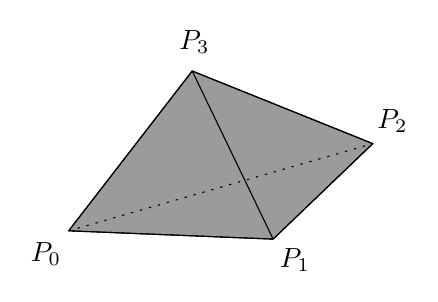
\begin{tikzpicture}[x=0.75pt,y=0.75pt,yscale=-1,xscale=1]
        %uncomment if require: \path (0,300); %set diagram left start at 0, and has height of 300

        %Shape: Polygon [id:ds9842074597762291] 
        \draw  [fill={rgb, 255:red, 155; green, 155; blue, 155 }  ,fill opacity=1 ] (246.5,83) -- (198.5,129) -- (100,125) -- (100,125) -- (159.5,48) -- cycle ;
        %Straight Lines [id:da9729295143022885] 
        \draw    (100,125) -- (198.5,129) ;
        %Straight Lines [id:da27501445764909294] 
        \draw    (100,125) -- (159.5,48) ;
        %Straight Lines [id:da5871038657961762] 
        \draw    (159.5,48) -- (198.5,129) ;
        %Straight Lines [id:da5622383145320506] 
        \draw    (198.5,129) -- (246.5,83) ;
        %Straight Lines [id:da6765618397957549] 
        \draw    (159.5,48) -- (246.5,83) ;
        %Straight Lines [id:da13091152666855876] 
        \draw  [dash pattern={on 0.84pt off 2.51pt}]  (100,125) -- (246.5,83) ;

        % Text Node
        \draw (80.5,129.4) node [anchor=north west][inner sep=0.75pt]    {$P_{0}$};
        % Text Node
        \draw (200.5,132.4) node [anchor=north west][inner sep=0.75pt]    {$P_{1}$};
        % Text Node
        \draw (247.5,65.4) node [anchor=north west][inner sep=0.75pt]    {$P_{2}$};
        % Text Node
        \draw (152,27.4) node [anchor=north west][inner sep=0.75pt]    {$P_{3}$};


    \end{tikzpicture}

\end{center}
\[
    \partial_3[P_0,P_1,P_2,P_3]=-[P_0,P_1,P_2]+[P_0,P_1,P_3]-[P_0,P_2,P_3]+[P_1,P_2,P_3]
\]
consideriamo i singoli termini
\begin{center}


    \tikzset{every picture/.style={line width=0.75pt}} %set default line width to 0.75pt        

    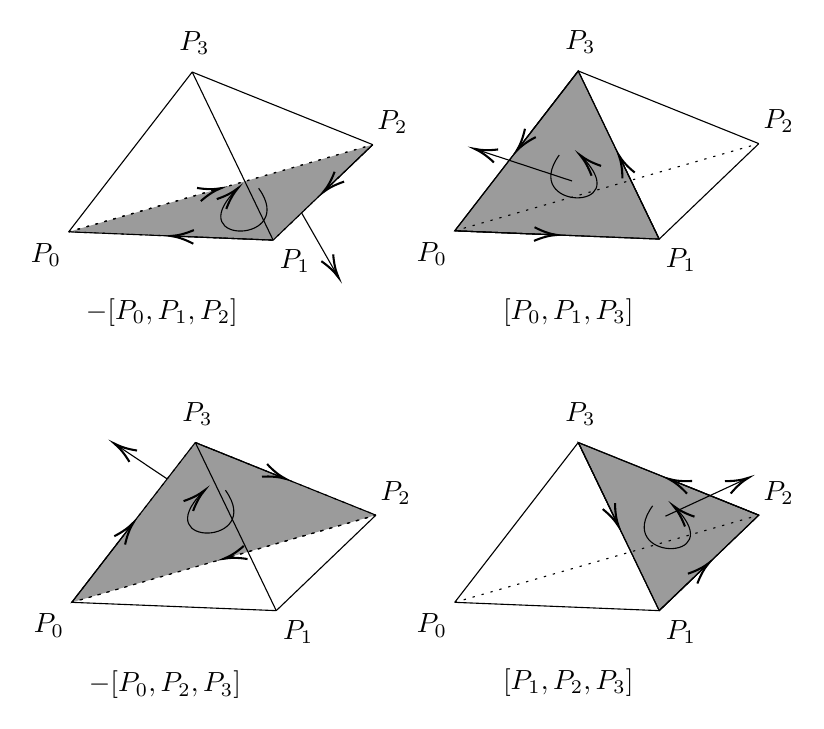
\begin{tikzpicture}[x=0.75pt,y=0.75pt,yscale=-1,xscale=1]
        %uncomment if require: \path (0,433); %set diagram left start at 0, and has height of 433

        %Straight Lines [id:da31119488772584236] 
        \draw    (110.5,236) -- (66.66,206.61) ;
        \draw [shift={(65,205.5)}, rotate = 33.84] [color={rgb, 255:red, 0; green, 0; blue, 0 }  ][line width=0.75]    (10.93,-3.29) .. controls (6.95,-1.4) and (3.31,-0.3) .. (0,0) .. controls (3.31,0.3) and (6.95,1.4) .. (10.93,3.29)   ;
        %Straight Lines [id:da0053318631895049595] 
        \draw    (149,83.5) -- (172.01,123.76) ;
        \draw [shift={(173,125.5)}, rotate = 240.26] [color={rgb, 255:red, 0; green, 0; blue, 0 }  ][line width=0.75]    (10.93,-3.29) .. controls (6.95,-1.4) and (3.31,-0.3) .. (0,0) .. controls (3.31,0.3) and (6.95,1.4) .. (10.93,3.29)   ;
        %Shape: Polygon [id:ds9842074597762291] 
        \draw  [fill={rgb, 255:red, 155; green, 155; blue, 155 }  ,fill opacity=1 ][dash pattern={on 0.84pt off 2.51pt}] (189.5,61.5) -- (141.5,107.5) -- (43,103.5) -- (43,103.5) -- (189.5,61.5) -- cycle ;
        %Straight Lines [id:da9729295143022885] 
        \draw    (43,103.5) -- (141.5,107.5) ;
        %Straight Lines [id:da27501445764909294] 
        \draw    (43,103.5) -- (102.5,26.5) ;
        %Straight Lines [id:da5871038657961762] 
        \draw    (102.5,26.5) -- (141.5,107.5) ;
        %Straight Lines [id:da5622383145320506] 
        \draw    (141.5,107.5) -- (189.5,61.5) ;
        %Straight Lines [id:da6765618397957549] 
        \draw    (102.5,26.5) -- (189.5,61.5) ;
        %Straight Lines [id:da13091152666855876] 
        \draw  [dash pattern={on 0.84pt off 2.51pt}]  (43,103.5) -- (189.5,61.5) ;
        %Shape: Polygon [id:ds7730849387300622] 
        \draw  [fill={rgb, 255:red, 155; green, 155; blue, 155 }  ,fill opacity=1 ] (288.5,26) -- (327.5,107) -- (229,103) -- (229,103) -- (288.5,26) -- cycle ;
        %Straight Lines [id:da7010360742157096] 
        \draw    (229,103) -- (327.5,107) ;
        %Straight Lines [id:da1247827305597089] 
        \draw    (229,103) -- (288.5,26) ;
        %Straight Lines [id:da9783698725241237] 
        \draw    (288.5,26) -- (327.5,107) ;
        %Straight Lines [id:da5121893168417577] 
        \draw    (327.5,107) -- (375.5,61) ;
        %Straight Lines [id:da05041247120115666] 
        \draw    (288.5,26) -- (375.5,61) ;
        %Straight Lines [id:da20111951070035605] 
        \draw  [dash pattern={on 0.84pt off 2.51pt}]  (229,103) -- (375.5,61) ;
        %Shape: Polygon [id:ds921910283108937] 
        \draw  [fill={rgb, 255:red, 155; green, 155; blue, 155 }  ,fill opacity=1 ][dash pattern={on 0.84pt off 2.51pt}] (191,240) -- (191,240) -- (44.5,282) -- (44.5,282) -- (104,205) -- cycle ;
        %Straight Lines [id:da4510645980675554] 
        \draw    (44.5,282) -- (143,286) ;
        %Straight Lines [id:da43780206861484117] 
        \draw    (44.5,282) -- (104,205) ;
        %Straight Lines [id:da1766600824533533] 
        \draw    (104,205) -- (143,286) ;
        %Straight Lines [id:da022271197569222467] 
        \draw    (143,286) -- (191,240) ;
        %Straight Lines [id:da5703279648644173] 
        \draw    (104,205) -- (191,240) ;
        %Straight Lines [id:da7416269976704115] 
        \draw  [dash pattern={on 0.84pt off 2.51pt}]  (44.5,282) -- (191,240) ;
        %Shape: Polygon [id:ds4253276718453256] 
        \draw  [fill={rgb, 255:red, 155; green, 155; blue, 155 }  ,fill opacity=1 ] (375.5,240) -- (327.5,286) -- (327.5,286) -- (327.5,286) -- (288.5,205) -- cycle ;
        %Straight Lines [id:da0889234805112924] 
        \draw    (229,282) -- (327.5,286) ;
        %Straight Lines [id:da9896200334014105] 
        \draw    (229,282) -- (288.5,205) ;
        %Straight Lines [id:da5641235690529702] 
        \draw    (288.5,205) -- (327.5,286) ;
        %Straight Lines [id:da7952476323856958] 
        \draw    (327.5,286) -- (375.5,240) ;
        %Straight Lines [id:da21029370192784325] 
        \draw    (288.5,205) -- (375.5,240) ;
        %Straight Lines [id:da6236013629909285] 
        \draw  [dash pattern={on 0.84pt off 2.51pt}]  (229,282) -- (375.5,240) ;
        %Straight Lines [id:da8871240250906955] 
        \draw  [dash pattern={on 0.84pt off 2.51pt}]  (43,103.5) -- (114.33,83.05) ;
        \draw [shift={(116.25,82.5)}, rotate = 164] [color={rgb, 255:red, 0; green, 0; blue, 0 }  ][line width=0.75]    (10.93,-3.29) .. controls (6.95,-1.4) and (3.31,-0.3) .. (0,0) .. controls (3.31,0.3) and (6.95,1.4) .. (10.93,3.29)   ;
        %Straight Lines [id:da2762721170088336] 
        \draw    (189.5,61.5) -- (166.94,83.12) ;
        \draw [shift={(165.5,84.5)}, rotate = 316.22] [color={rgb, 255:red, 0; green, 0; blue, 0 }  ][line width=0.75]    (10.93,-3.29) .. controls (6.95,-1.4) and (3.31,-0.3) .. (0,0) .. controls (3.31,0.3) and (6.95,1.4) .. (10.93,3.29)   ;
        %Straight Lines [id:da1643264021198394] 
        \draw    (141.5,107.5) -- (94.25,105.58) ;
        \draw [shift={(92.25,105.5)}, rotate = 2.33] [color={rgb, 255:red, 0; green, 0; blue, 0 }  ][line width=0.75]    (10.93,-3.29) .. controls (6.95,-1.4) and (3.31,-0.3) .. (0,0) .. controls (3.31,0.3) and (6.95,1.4) .. (10.93,3.29)   ;
        %Straight Lines [id:da2804942378736206] 
        \draw    (288.5,26) -- (259.97,62.92) ;
        \draw [shift={(258.75,64.5)}, rotate = 307.69] [color={rgb, 255:red, 0; green, 0; blue, 0 }  ][line width=0.75]    (10.93,-3.29) .. controls (6.95,-1.4) and (3.31,-0.3) .. (0,0) .. controls (3.31,0.3) and (6.95,1.4) .. (10.93,3.29)   ;
        %Straight Lines [id:da7410796519703213] 
        \draw    (229,103) -- (276.25,104.92) ;
        \draw [shift={(278.25,105)}, rotate = 182.33] [color={rgb, 255:red, 0; green, 0; blue, 0 }  ][line width=0.75]    (10.93,-3.29) .. controls (6.95,-1.4) and (3.31,-0.3) .. (0,0) .. controls (3.31,0.3) and (6.95,1.4) .. (10.93,3.29)   ;
        %Straight Lines [id:da2995632170944471] 
        \draw    (327.5,107) -- (308.87,68.3) ;
        \draw [shift={(308,66.5)}, rotate = 64.29] [color={rgb, 255:red, 0; green, 0; blue, 0 }  ][line width=0.75]    (10.93,-3.29) .. controls (6.95,-1.4) and (3.31,-0.3) .. (0,0) .. controls (3.31,0.3) and (6.95,1.4) .. (10.93,3.29)   ;
        %Straight Lines [id:da806982694486216] 
        \draw  [dash pattern={on 0.84pt off 2.51pt}]  (191,240) -- (119.67,260.45) ;
        \draw [shift={(117.75,261)}, rotate = 344] [color={rgb, 255:red, 0; green, 0; blue, 0 }  ][line width=0.75]    (10.93,-3.29) .. controls (6.95,-1.4) and (3.31,-0.3) .. (0,0) .. controls (3.31,0.3) and (6.95,1.4) .. (10.93,3.29)   ;
        %Straight Lines [id:da37720849745808827] 
        \draw    (104,205) -- (145.64,221.75) ;
        \draw [shift={(147.5,222.5)}, rotate = 201.91] [color={rgb, 255:red, 0; green, 0; blue, 0 }  ][line width=0.75]    (10.93,-3.29) .. controls (6.95,-1.4) and (3.31,-0.3) .. (0,0) .. controls (3.31,0.3) and (6.95,1.4) .. (10.93,3.29)   ;
        %Straight Lines [id:da4049776429406269] 
        \draw    (44.5,282) -- (73.03,245.08) ;
        \draw [shift={(74.25,243.5)}, rotate = 127.69] [color={rgb, 255:red, 0; green, 0; blue, 0 }  ][line width=0.75]    (10.93,-3.29) .. controls (6.95,-1.4) and (3.31,-0.3) .. (0,0) .. controls (3.31,0.3) and (6.95,1.4) .. (10.93,3.29)   ;
        %Straight Lines [id:da5023281466268048] 
        \draw    (288.5,205) -- (307.13,243.7) ;
        \draw [shift={(308,245.5)}, rotate = 244.29] [color={rgb, 255:red, 0; green, 0; blue, 0 }  ][line width=0.75]    (10.93,-3.29) .. controls (6.95,-1.4) and (3.31,-0.3) .. (0,0) .. controls (3.31,0.3) and (6.95,1.4) .. (10.93,3.29)   ;
        %Straight Lines [id:da18898800798826576] 
        \draw    (327.5,286) -- (350.06,264.38) ;
        \draw [shift={(351.5,263)}, rotate = 136.22] [color={rgb, 255:red, 0; green, 0; blue, 0 }  ][line width=0.75]    (10.93,-3.29) .. controls (6.95,-1.4) and (3.31,-0.3) .. (0,0) .. controls (3.31,0.3) and (6.95,1.4) .. (10.93,3.29)   ;
        %Straight Lines [id:da6783592735518349] 
        \draw    (375.5,240) -- (333.86,223.25) ;
        \draw [shift={(332,222.5)}, rotate = 21.91] [color={rgb, 255:red, 0; green, 0; blue, 0 }  ][line width=0.75]    (10.93,-3.29) .. controls (6.95,-1.4) and (3.31,-0.3) .. (0,0) .. controls (3.31,0.3) and (6.95,1.4) .. (10.93,3.29)   ;
        %Shape: Boxed Bezier Curve [id:dp8334283236635056] 
        \draw    (279.34,66.5) .. controls (260.13,93.1) and (316.6,94.46) .. (290.59,67.74) ;
        \draw [shift={(289.34,66.5)}, rotate = 43.99] [color={rgb, 255:red, 0; green, 0; blue, 0 }  ][line width=0.75]    (10.93,-3.29) .. controls (6.95,-1.4) and (3.31,-0.3) .. (0,0) .. controls (3.31,0.3) and (6.95,1.4) .. (10.93,3.29)   ;
        %Curve Lines [id:da12332707576636937] 
        \draw    (134.5,82.5) .. controls (153.71,109.1) and (97.24,110.46) .. (123.25,83.74) ;
        \draw [shift={(124.5,82.5)}, rotate = 136.01] [color={rgb, 255:red, 0; green, 0; blue, 0 }  ][line width=0.75]    (10.93,-3.29) .. controls (6.95,-1.4) and (3.31,-0.3) .. (0,0) .. controls (3.31,0.3) and (6.95,1.4) .. (10.93,3.29)   ;
        %Curve Lines [id:da4656956479773615] 
        \draw    (118.5,228) .. controls (137.71,254.6) and (81.24,255.96) .. (107.25,229.24) ;
        \draw [shift={(108.5,228)}, rotate = 136.01] [color={rgb, 255:red, 0; green, 0; blue, 0 }  ][line width=0.75]    (10.93,-3.29) .. controls (6.95,-1.4) and (3.31,-0.3) .. (0,0) .. controls (3.31,0.3) and (6.95,1.4) .. (10.93,3.29)   ;
        %Shape: Boxed Bezier Curve [id:dp8286852342613502] 
        \draw    (324.34,235.5) .. controls (305.13,262.1) and (361.6,263.46) .. (335.59,236.74) ;
        \draw [shift={(334.34,235.5)}, rotate = 43.99] [color={rgb, 255:red, 0; green, 0; blue, 0 }  ][line width=0.75]    (10.93,-3.29) .. controls (6.95,-1.4) and (3.31,-0.3) .. (0,0) .. controls (3.31,0.3) and (6.95,1.4) .. (10.93,3.29)   ;
        %Straight Lines [id:da996112223083482] 
        \draw    (285.5,79) -- (240.4,64.13) ;
        \draw [shift={(238.5,63.5)}, rotate = 18.25] [color={rgb, 255:red, 0; green, 0; blue, 0 }  ][line width=0.75]    (10.93,-3.29) .. controls (6.95,-1.4) and (3.31,-0.3) .. (0,0) .. controls (3.31,0.3) and (6.95,1.4) .. (10.93,3.29)   ;
        %Straight Lines [id:da24337164617945461] 
        \draw    (330.5,240.5) -- (368.68,222.84) ;
        \draw [shift={(370.5,222)}, rotate = 155.18] [color={rgb, 255:red, 0; green, 0; blue, 0 }  ][line width=0.75]    (10.93,-3.29) .. controls (6.95,-1.4) and (3.31,-0.3) .. (0,0) .. controls (3.31,0.3) and (6.95,1.4) .. (10.93,3.29)   ;

        % Text Node
        \draw (23.5,107.9) node [anchor=north west][inner sep=0.75pt]    {$P_{0}$};
        % Text Node
        \draw (143.5,110.9) node [anchor=north west][inner sep=0.75pt]    {$P_{1}$};
        % Text Node
        \draw (190.5,43.9) node [anchor=north west][inner sep=0.75pt]    {$P_{2}$};
        % Text Node
        \draw (95,5.9) node [anchor=north west][inner sep=0.75pt]    {$P_{3}$};
        % Text Node
        \draw (209.5,107.4) node [anchor=north west][inner sep=0.75pt]    {$P_{0}$};
        % Text Node
        \draw (329.5,110.4) node [anchor=north west][inner sep=0.75pt]    {$P_{1}$};
        % Text Node
        \draw (376.5,43.4) node [anchor=north west][inner sep=0.75pt]    {$P_{2}$};
        % Text Node
        \draw (281,5.4) node [anchor=north west][inner sep=0.75pt]    {$P_{3}$};
        % Text Node
        \draw (25,286.4) node [anchor=north west][inner sep=0.75pt]    {$P_{0}$};
        % Text Node
        \draw (145,289.4) node [anchor=north west][inner sep=0.75pt]    {$P_{1}$};
        % Text Node
        \draw (192,222.4) node [anchor=north west][inner sep=0.75pt]    {$P_{2}$};
        % Text Node
        \draw (96.5,184.4) node [anchor=north west][inner sep=0.75pt]    {$P_{3}$};
        % Text Node
        \draw (209.5,286.4) node [anchor=north west][inner sep=0.75pt]    {$P_{0}$};
        % Text Node
        \draw (329.5,289.4) node [anchor=north west][inner sep=0.75pt]    {$P_{1}$};
        % Text Node
        \draw (376.5,222.4) node [anchor=north west][inner sep=0.75pt]    {$P_{2}$};
        % Text Node
        \draw (281,184.4) node [anchor=north west][inner sep=0.75pt]    {$P_{3}$};
        % Text Node
        \draw (50,134.4) node [anchor=north west][inner sep=0.75pt]    {$-[ P_{0} ,P_{1} ,P_{2}]$};
        % Text Node
        \draw (251,134.4) node [anchor=north west][inner sep=0.75pt]    {$[ P_{0} ,P_{1} ,P_{3}]$};
        % Text Node
        \draw (51.5,313.9) node [anchor=north west][inner sep=0.75pt]    {$-[ P_{0} ,P_{2} ,P_{3}]$};
        % Text Node
        \draw (251,312.9) node [anchor=north west][inner sep=0.75pt]    {$[ P_{1} ,P_{2} ,P_{3}]$};


    \end{tikzpicture}

\end{center}
L'operatore di bordo rappresenta un flusso uscente dal solido
\paragraph{Osservazione} Ogni lato del 3-bordo di $[P_0,P_1,P_2,P_3]$ è percorso due volte, in versi opposti
\begin{theorem}
    Sia $K$ un complessso simpliciale, la composizione di due operatori bordo consecutivi è uguale all'omomorfismo nullo
    \[
        \partial_{p_1}\circ\partial_p=0\quad\forall p
    \]
\end{theorem}
\begin{proof}
    Osservo che se $p>dim\ K$ oppure $p-1\leq 0\implies p\leq 1$, allora uno dei due omomorfismi $\partial$ oppure $\partial_{p-1}$ è l'omomorfismo nullo, la composizione è quindi banalmente l'omomorfismo nullo\\
    Nel caso $1<p\leq dim\ K$, studio gli effetti la composizione degli operatori bordo sulla base del gruppo $C_p(K)$
    \[
        \partial_{p-1}\left(\partial_p[P_0,\dots,P_p]\right)=\partial_{p-1}\left(\sum_{i=0}^p(-1)^i[P_0,\dots,P_{i-1},\hat{P_i},P_{i+1},\dots,P_p]\right)=
    \]
    \[
        =\sum_{i=0}^p(-1)^i\partial_{p-1}[P_0,\dots,P_{i-1},\hat{P_i},P_{i+1},\dots,P_p]
    \]
    possiamo spezzare la somma nei due casi possibili dell'applicazione del secondo operatore bordo (rimuovo un punto prima di $P_i$, oppure dopo $P_i$)
    \[
        =\sum_{j<i}(-1)^i(-1)^j[P_0,\dots,\hat{P_j},\dots,\hat{P_i},\dots,P_p]+
    \]
    \[
        +\sum_{j>i}(-1)^i(-1)^{j-1}[P_0,\dots,\hat{P_i},\dots,\hat{P_j},\dots,P_p]
    \]
    (poichè rimuovo un elemento prima di $P_j$, l'indice risulta spostato)\\
    Ottengo quindi
    \[
        =\sum_{j<i}(-1)^{i+j}[P_0,\dots,\hat{P_j},\dots,\hat{P_i},\dots,P_p]
    \]
    \[
        -\sum_{j>i}(-1)^{i+j}[P_0,\dots,\hat{P_i},\dots,\hat{P_j},\dots,P_p]
    \]
    \[
        =0
    \]
\end{proof}
Segue quindi un corollario, facilmente rappresentabile con un diagramma
\pagebreak
\begin{corollary}
    Sia $K$ un complesso simpliciale, il seguente diagramma commuta
    \begin{center}
        \adjustbox{scale=0.7,center}{%
            \begin{tikzcd}
                \dots && {C_{p+1}(K)} && {C_p(K)} && \dots && {C_3(K)} && {C_2(K)} && {C_1(K)} && {C_0(K)} && 0
                \arrow["{\partial_{p+2}}", from=1-1, to=1-3]
                \arrow["{\partial_{p+1}}", from=1-3, to=1-5]
                \arrow["{\partial_p}", from=1-5, to=1-7]
                \arrow["{\partial_4}", from=1-7, to=1-9]
                \arrow["{\partial_3}", from=1-9, to=1-11]
                \arrow["{\partial_2}", from=1-11, to=1-13]
                \arrow["{\partial_1}", from=1-13, to=1-15]
                \arrow["{\partial_0}", from=1-15, to=1-17]
                \arrow["0"', curve={height=30pt}, from=1-1, to=1-5]
                \arrow["0", curve={height=-30pt}, from=1-3, to=1-7]
                \arrow["0"', curve={height=30pt}, from=1-9, to=1-13]
                \arrow["0", curve={height=-30pt}, from=1-11, to=1-15]
                \arrow["0"', curve={height=30pt}, from=1-13, to=1-17]
            \end{tikzcd}
        }
    \end{center}
    Inoltre
    \[
        \partial_{p-1}\circ\partial_p=0\implies Im(\partial)\subseteq Ker(\partial_{p-1})
    \]
\end{corollary}
\paragraph{Domanda} "Misurare" la differenza tra $Im(\partial_p)$ e $Ker(\partial_{p-1})$ ci dà delle informazioni sulla topologia del complesso?
\begin{definition}[Gruppo dei p-cicli]
    Il nucleo dell'operatore bordo $\partial_p:C_p(K)\ra C_{p-1}(K)$ su un complesso simpliciale $K$ si dice gruppo dei p-cicli di $K$ e viene denotato con
    \[
        Z_p(K)
    \]
\end{definition}
\begin{definition}[Gruppo dei p-bordi]
    L'immagine dell'operatore bordo $\partial_{p+1}:C_{p+1}(K)\ra C_{p}(K)$ su un complesso simpliciale $K$ si dice gruppo dei p-bordi di $K$ e viene denotato con
    \[
        B_p(K)
    \]
\end{definition}
\paragraph{Osservazione}
Per il corollario, abbiamo
\[
    B_p(K)\subseteq Z_p(K)\subseteq C_p(K)
\]
il che spiega la scelta degli indici diversi per i p-cicli e i p-bordi
\begin{definition}[Gruppi di omologia]
    Dato un complesso simpliciale $K$, chiamiamo p-esimo gruppo di omologia (simpliciale) di $K$ il gruppo
    \[
        H_p(K):=\faktor{Z_p(K)}{B_p(K)}
    \]
\end{definition}
\pagebreak
\section{Esempio completo}
Calcolare i gruppi di omologia simpliciale del complesso simpliciale
\[
    K=\{[P_0,P_1],[P_1,P_2],[P_2,P_3],[P_0,P_3],P_0,P_1,P_2,P_3\}
\]
\begin{center}


    \tikzset{every picture/.style={line width=0.75pt}} %set default line width to 0.75pt        

    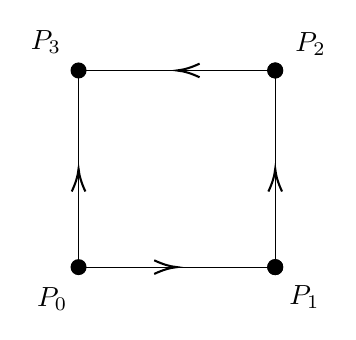
\begin{tikzpicture}[x=0.75pt,y=0.75pt,yscale=-1,xscale=1]
        %uncomment if require: \path (0,433); %set diagram left start at 0, and has height of 433

        %Shape: Square [id:dp311972140197708] 
        \draw   (76.25,40.75) -- (171,40.75) -- (171,135.5) -- (76.25,135.5) -- cycle ;
        %Straight Lines [id:da3375767366574549] 
        \draw    (76.25,40.75) -- (171,40.75) ;
        \draw [shift={(171,40.75)}, rotate = 0] [color={rgb, 255:red, 0; green, 0; blue, 0 }  ][fill={rgb, 255:red, 0; green, 0; blue, 0 }  ][line width=0.75]      (0, 0) circle [x radius= 3.35, y radius= 3.35]   ;
        \draw [shift={(76.25,40.75)}, rotate = 0] [color={rgb, 255:red, 0; green, 0; blue, 0 }  ][fill={rgb, 255:red, 0; green, 0; blue, 0 }  ][line width=0.75]      (0, 0) circle [x radius= 3.35, y radius= 3.35]   ;
        %Straight Lines [id:da9195953727513981] 
        \draw    (76.25,135.5) -- (171,135.5) ;
        \draw [shift={(171,135.5)}, rotate = 0] [color={rgb, 255:red, 0; green, 0; blue, 0 }  ][fill={rgb, 255:red, 0; green, 0; blue, 0 }  ][line width=0.75]      (0, 0) circle [x radius= 3.35, y radius= 3.35]   ;
        \draw [shift={(76.25,135.5)}, rotate = 0] [color={rgb, 255:red, 0; green, 0; blue, 0 }  ][fill={rgb, 255:red, 0; green, 0; blue, 0 }  ][line width=0.75]      (0, 0) circle [x radius= 3.35, y radius= 3.35]   ;
        %Straight Lines [id:da8059513303813619] 
        \draw    (76.25,135.5) -- (121.63,135.5) ;
        \draw [shift={(123.63,135.5)}, rotate = 180] [color={rgb, 255:red, 0; green, 0; blue, 0 }  ][line width=0.75]    (10.93,-3.29) .. controls (6.95,-1.4) and (3.31,-0.3) .. (0,0) .. controls (3.31,0.3) and (6.95,1.4) .. (10.93,3.29)   ;
        %Straight Lines [id:da2285831064146353] 
        \draw    (76.25,135.5) -- (76.25,40.75) ;
        %Straight Lines [id:da6732465533433227] 
        \draw    (76.25,135.5) -- (76.25,90.13) ;
        \draw [shift={(76.25,88.13)}, rotate = 90] [color={rgb, 255:red, 0; green, 0; blue, 0 }  ][line width=0.75]    (10.93,-3.29) .. controls (6.95,-1.4) and (3.31,-0.3) .. (0,0) .. controls (3.31,0.3) and (6.95,1.4) .. (10.93,3.29)   ;
        %Straight Lines [id:da06827916766160635] 
        \draw    (171,40.75) -- (125.63,40.75) ;
        \draw [shift={(123.63,40.75)}, rotate = 360] [color={rgb, 255:red, 0; green, 0; blue, 0 }  ][line width=0.75]    (10.93,-3.29) .. controls (6.95,-1.4) and (3.31,-0.3) .. (0,0) .. controls (3.31,0.3) and (6.95,1.4) .. (10.93,3.29)   ;
        %Straight Lines [id:da8480868265281654] 
        \draw    (171,40.75) -- (171,135.5) ;
        \draw [shift={(171,135.5)}, rotate = 90] [color={rgb, 255:red, 0; green, 0; blue, 0 }  ][fill={rgb, 255:red, 0; green, 0; blue, 0 }  ][line width=0.75]      (0, 0) circle [x radius= 3.35, y radius= 3.35]   ;
        \draw [shift={(171,40.75)}, rotate = 90] [color={rgb, 255:red, 0; green, 0; blue, 0 }  ][fill={rgb, 255:red, 0; green, 0; blue, 0 }  ][line width=0.75]      (0, 0) circle [x radius= 3.35, y radius= 3.35]   ;
        %Straight Lines [id:da8783982634233514] 
        \draw    (171,135.5) -- (171,90.13) ;
        \draw [shift={(171,88.13)}, rotate = 90] [color={rgb, 255:red, 0; green, 0; blue, 0 }  ][line width=0.75]    (10.93,-3.29) .. controls (6.95,-1.4) and (3.31,-0.3) .. (0,0) .. controls (3.31,0.3) and (6.95,1.4) .. (10.93,3.29)   ;

        % Text Node
        \draw (55,143.9) node [anchor=north west][inner sep=0.75pt]    {$P_{0}$};
        % Text Node
        \draw (176.5,142.9) node [anchor=north west][inner sep=0.75pt]    {$P_{1}$};
        % Text Node
        \draw (179.5,21.4) node [anchor=north west][inner sep=0.75pt]    {$P_{2}$};
        % Text Node
        \draw (52,20.4) node [anchor=north west][inner sep=0.75pt]    {$P_{3}$};


    \end{tikzpicture}

\end{center}
\subsection{Step 1: Calcolo p-catene}
\begin{itemize}
    \item $C_0(K)=\gen{P_0,P_1,P_2,P_3}\simeq\Z^4$
    \item $C_1(K)=\gen{[P_0,P_1],[P_1,P_2],[P_2,P_3],[P_0,P_3]}\simeq\Z^4$
    \item $C_p(K)=\{0\}$ $\forall p\neq0,1$
\end{itemize}
Avrò quindi 2 gruppi di omologia
\subsection{Step 2: Operatori bordo}
\begin{itemize}
    \item $\partial_p=0$ $\forall p\neq 1$
    \item $\partial_1:C_1(K)\ra C_0(K)$
          \[
              \partial_1=\left[\begin{array}{rrrr}
                      -1 & 0  & 0  & -1 \\
                      1  & -1 & 0  & 0  \\
                      0  & 1  & -1 & 0  \\
                      0  & 0  & 1  & 1
                  \end{array}\right]
          \]
\end{itemize}
\subsection{Step 3: Determinare p-cicli e p-bordi}
\paragraph{p=0}
\[
    H_0(K)=\faktor{Z_0(K)}{B_0(K)}=\faktor{Ker\ \partial_0}{Im\ \partial_1}
\]
\[
    \partial_0:C_0(K)\ra\{0\}\implies\partial_0=0\implies Z_0(K)=C_0(K)
\]
Per quanto riguarda $B_0(K)$, esso è generato dalle immagini della base di $C_1(K)$ tramite $\partial_1$
\[
    \partial_1[P_0,P_1]=P_1-P_0
\]
\[
    \partial_1[P_1,P_2]=P_2-P_1
\]
\[
    \partial_1[P_2,P_3]=P_3-P_2
\]
\[
    \partial_1[P_0,P_3]=P_3-P_1
\]
\pagebreak
Questi generatori sono minimali? Dobbiamo risolvere
\[
    m_1(P_1-P_0)+m_2(P_2-P_1)+m_3(P_3-P_2)+m_4(P_0-P_3)=0
\]
e troviamo che il quarto generatore è rindondante.\\
Abbiamo quindi
\[
    B_0(K)=\gen{P_1-P_0,P_2-P_1,P_3-P_2}\simeq\Z^3
\]
\subparagraph{Osservazione}
Dal disegno si intuiva che $[P_0,P_3]$ era ridondante, infatti
\begin{center}


    \tikzset{every picture/.style={line width=0.75pt}} %set default line width to 0.75pt        

    \begin{tikzpicture}[x=0.75pt,y=0.75pt,yscale=-1,xscale=1]
        %uncomment if require: \path (0,433); %set diagram left start at 0, and has height of 433

        %Shape: Square [id:dp311972140197708] 
        \draw   (162.75,39.75) -- (257.5,39.75) -- (257.5,134.5) -- (162.75,134.5) -- cycle ;
        %Straight Lines [id:da3375767366574549] 
        \draw    (162.75,39.75) -- (257.5,39.75) ;
        \draw [shift={(257.5,39.75)}, rotate = 0] [color={rgb, 255:red, 0; green, 0; blue, 0 }  ][fill={rgb, 255:red, 0; green, 0; blue, 0 }  ][line width=0.75]      (0, 0) circle [x radius= 3.35, y radius= 3.35]   ;
        \draw [shift={(162.75,39.75)}, rotate = 0] [color={rgb, 255:red, 0; green, 0; blue, 0 }  ][fill={rgb, 255:red, 0; green, 0; blue, 0 }  ][line width=0.75]      (0, 0) circle [x radius= 3.35, y radius= 3.35]   ;
        %Straight Lines [id:da9195953727513981] 
        \draw    (162.75,134.5) -- (257.5,134.5) ;
        \draw [shift={(257.5,134.5)}, rotate = 0] [color={rgb, 255:red, 0; green, 0; blue, 0 }  ][fill={rgb, 255:red, 0; green, 0; blue, 0 }  ][line width=0.75]      (0, 0) circle [x radius= 3.35, y radius= 3.35]   ;
        \draw [shift={(162.75,134.5)}, rotate = 0] [color={rgb, 255:red, 0; green, 0; blue, 0 }  ][fill={rgb, 255:red, 0; green, 0; blue, 0 }  ][line width=0.75]      (0, 0) circle [x radius= 3.35, y radius= 3.35]   ;
        %Straight Lines [id:da8059513303813619] 
        \draw    (162.75,134.5) -- (208.13,134.5) ;
        \draw [shift={(210.13,134.5)}, rotate = 180] [color={rgb, 255:red, 0; green, 0; blue, 0 }  ][line width=0.75]    (10.93,-3.29) .. controls (6.95,-1.4) and (3.31,-0.3) .. (0,0) .. controls (3.31,0.3) and (6.95,1.4) .. (10.93,3.29)   ;
        %Straight Lines [id:da2285831064146353] 
        \draw    (162.75,134.5) -- (162.75,39.75) ;
        %Straight Lines [id:da6732465533433227] 
        \draw    (162.75,134.5) -- (162.75,89.13) ;
        \draw [shift={(162.75,87.13)}, rotate = 90] [color={rgb, 255:red, 0; green, 0; blue, 0 }  ][line width=0.75]    (10.93,-3.29) .. controls (6.95,-1.4) and (3.31,-0.3) .. (0,0) .. controls (3.31,0.3) and (6.95,1.4) .. (10.93,3.29)   ;
        %Straight Lines [id:da06827916766160635] 
        \draw    (257.5,39.75) -- (212.13,39.75) ;
        \draw [shift={(210.13,39.75)}, rotate = 360] [color={rgb, 255:red, 0; green, 0; blue, 0 }  ][line width=0.75]    (10.93,-3.29) .. controls (6.95,-1.4) and (3.31,-0.3) .. (0,0) .. controls (3.31,0.3) and (6.95,1.4) .. (10.93,3.29)   ;
        %Straight Lines [id:da8480868265281654] 
        \draw    (257.5,39.75) -- (257.5,134.5) ;
        \draw [shift={(257.5,134.5)}, rotate = 90] [color={rgb, 255:red, 0; green, 0; blue, 0 }  ][fill={rgb, 255:red, 0; green, 0; blue, 0 }  ][line width=0.75]      (0, 0) circle [x radius= 3.35, y radius= 3.35]   ;
        \draw [shift={(257.5,39.75)}, rotate = 90] [color={rgb, 255:red, 0; green, 0; blue, 0 }  ][fill={rgb, 255:red, 0; green, 0; blue, 0 }  ][line width=0.75]      (0, 0) circle [x radius= 3.35, y radius= 3.35]   ;
        %Straight Lines [id:da8783982634233514] 
        \draw    (257.5,134.5) -- (257.5,89.13) ;
        \draw [shift={(257.5,87.13)}, rotate = 90] [color={rgb, 255:red, 0; green, 0; blue, 0 }  ][line width=0.75]    (10.93,-3.29) .. controls (6.95,-1.4) and (3.31,-0.3) .. (0,0) .. controls (3.31,0.3) and (6.95,1.4) .. (10.93,3.29)   ;
        %Straight Lines [id:da6676738876618311] 
        \draw  [dash pattern={on 0.84pt off 2.51pt}]  (396.25,39.25) -- (491,39.25) ;
        \draw [shift={(491,39.25)}, rotate = 0] [color={rgb, 255:red, 0; green, 0; blue, 0 }  ][fill={rgb, 255:red, 0; green, 0; blue, 0 }  ][line width=0.75]      (0, 0) circle [x radius= 3.35, y radius= 3.35]   ;
        \draw [shift={(396.25,39.25)}, rotate = 0] [color={rgb, 255:red, 0; green, 0; blue, 0 }  ][fill={rgb, 255:red, 0; green, 0; blue, 0 }  ][line width=0.75]      (0, 0) circle [x radius= 3.35, y radius= 3.35]   ;
        %Straight Lines [id:da4179317562637974] 
        \draw  [dash pattern={on 0.84pt off 2.51pt}]  (396.25,134) -- (491,134) ;
        \draw [shift={(491,134)}, rotate = 0] [color={rgb, 255:red, 0; green, 0; blue, 0 }  ][fill={rgb, 255:red, 0; green, 0; blue, 0 }  ][line width=0.75]      (0, 0) circle [x radius= 3.35, y radius= 3.35]   ;
        \draw [shift={(396.25,134)}, rotate = 0] [color={rgb, 255:red, 0; green, 0; blue, 0 }  ][fill={rgb, 255:red, 0; green, 0; blue, 0 }  ][line width=0.75]      (0, 0) circle [x radius= 3.35, y radius= 3.35]   ;
        %Straight Lines [id:da8083095145150079] 
        \draw  [dash pattern={on 0.84pt off 2.51pt}]  (491,39.25) -- (491,134) ;
        \draw [shift={(491,134)}, rotate = 90] [color={rgb, 255:red, 0; green, 0; blue, 0 }  ][fill={rgb, 255:red, 0; green, 0; blue, 0 }  ][line width=0.75]      (0, 0) circle [x radius= 3.35, y radius= 3.35]   ;
        \draw [shift={(491,39.25)}, rotate = 90] [color={rgb, 255:red, 0; green, 0; blue, 0 }  ][fill={rgb, 255:red, 0; green, 0; blue, 0 }  ][line width=0.75]      (0, 0) circle [x radius= 3.35, y radius= 3.35]   ;
        %Curve Lines [id:da705460979795109] 
        \draw    (396.25,134) .. controls (358.14,97.62) and (359.22,77.65) .. (395.15,40.38) ;
        \draw [shift={(396.25,39.25)}, rotate = 134.24] [color={rgb, 255:red, 0; green, 0; blue, 0 }  ][line width=0.75]    (10.93,-3.29) .. controls (6.95,-1.4) and (3.31,-0.3) .. (0,0) .. controls (3.31,0.3) and (6.95,1.4) .. (10.93,3.29)   ;
        %Curve Lines [id:da3225657442653589] 
        \draw    (396.25,134) .. controls (526.75,199.25) and (601.25,-5.25) .. (396.25,39.25) ;
        \draw [shift={(396.25,39.25)}, rotate = 347.75] [color={rgb, 255:red, 0; green, 0; blue, 0 }  ][line width=0.75]    (10.93,-3.29) .. controls (6.95,-1.4) and (3.31,-0.3) .. (0,0) .. controls (3.31,0.3) and (6.95,1.4) .. (10.93,3.29)   ;
        %Straight Lines [id:da11834010558175811] 
        \draw  [dash pattern={on 0.84pt off 2.51pt}]  (396.25,134) -- (396.25,39.25) ;
        %Straight Lines [id:da3416029770593103] 
        \draw    (287.25,89.75) -- (353.75,89.75) ;
        \draw [shift={(355.75,89.75)}, rotate = 180] [color={rgb, 255:red, 0; green, 0; blue, 0 }  ][line width=0.75]    (10.93,-3.29) .. controls (6.95,-1.4) and (3.31,-0.3) .. (0,0) .. controls (3.31,0.3) and (6.95,1.4) .. (10.93,3.29)   ;

        % Text Node
        \draw (141.5,142.9) node [anchor=north west][inner sep=0.75pt]    {$P_{0}$};
        % Text Node
        \draw (263,141.9) node [anchor=north west][inner sep=0.75pt]    {$P_{1}$};
        % Text Node
        \draw (266,20.4) node [anchor=north west][inner sep=0.75pt]    {$P_{2}$};
        % Text Node
        \draw (138.5,19.4) node [anchor=north west][inner sep=0.75pt]    {$P_{3}$};
        % Text Node
        \draw (375,142.4) node [anchor=north west][inner sep=0.75pt]    {$P_{0}$};
        % Text Node
        \draw (496.5,141.4) node [anchor=north west][inner sep=0.75pt]    {$P_{1}$};
        % Text Node
        \draw (499.5,19.9) node [anchor=north west][inner sep=0.75pt]    {$P_{2}$};
        % Text Node
        \draw (372,18.9) node [anchor=north west][inner sep=0.75pt]    {$P_{3}$};


    \end{tikzpicture}

\end{center}
$[P_0,P_3]$ non è l'unico modo per passare da $P_0$ a $P_3$\\
Come calcolo il quoziente?
\[
    \faktor{C_0(K)}{B_0(K)}=\faktor{\gen{P_0,P_1,P_2,P_3}}{\gen{P_1-P_0,P_2-P_1,P_3-P_2}}\simeq\faktor{\Z^4}{\Z^3}
\]
Ricordo che gli elementi di $\faktor{C_0(K)}{B_0(K)}$ sono le classi di equivalenza della relazione
\[
    a_0P_0+a_1P_1+a_2P_2+a_3P_3\sim b_0P_0+b_1P_1+b_2P_2+b_3P_3
\]
\[
    \Updownarrow
\]
\[
    (a_0-b_0)P_0+(a_1-b_1)P_1+(a_2-b_2)P_2+(a_3-b_3)P_3\in B_0(K)
\]
per descrivere le classi di equivalenza è utile determinare un rappresentante canonico ("speciale")
\[
    [a_0P_0+a_1P_1+a_2P_2+a_3P_3]\in H_0(K)
\]
\[
    \Updownarrow
\]
\[
    [a_0P_0+a_1P_1+a_2P_2+a_3P_3+\underbrace{(P_3-P_2)(-a_3)}_{\in B_0(K)}]\in H_0(K)
\]
\[
    \Updownarrow
\]
\[
    [a_0P_0+a_1P_1+(a_2+a_3)P_2\underbrace{-(a_2+a_3)(P_2-P_1)}_{\in B_0(K)}]\in H_0(K)
\]
\[
    \Updownarrow
\]
\[
    [a_0P_0+(a_1+a_2+a_3)P_1\underbrace{-(a_1+a_2+a_3)(P_1-P_0)}_{\in B_0(K)}]\in H_0(K)
\]
\[
    \Updownarrow
\]
\[
    [(a_0+a_1+a_2+a_3)P_0]\in H_0(K)
\]
ho (non rigorosamente) dimostrato che il quoziente ha un solo generatore, ossia $H_0(K)\simeq\Z$.\\
Per una dimostrazione algebrica, utilizzo il teorema fondamentale di isomorfismo. Considero il morfismo
\[
    f:C_0(K)\ra\Z
\]
\[
    a_0P_0+a_1P_1+a_2P_2+a_3P_3\longmapsto a_0+a_1+a_2+a_3
\]
la suriettività è banale. Segue inoltre che
\[
    Im\ f=\Z\quad Ker\ f=\gen{P_3-P_0,P_2-P_1,P_3-P_2}
\]
da cui
\[
    H_0(K)=\faktor{C_0(K)}{B_0(K)}=\faktor{C_0(K)}{Ker\ f}\simeq\Z
\]
\paragraph{p=1}
\[
    H_1(K)=\faktor{Z_1(K)}{B_1(K)}=\faktor{Ker\ \partial_1}{Im\ \partial_2}
\]
\[
    \partial_2:C_2(K)\ra C_1(K)
\]
poichè $C_2(K)=\{0\}$, è immediato $Im\ \partial_2=\{0\}$, da cui
\[
    H_1(K)=\faktor{Z_1(K)}{\{0\}}=Z_1(K)
\]
Calcoliamo il gruppo degli 1-cicli
\[
    Z_1(K)=Ker\ \partial_1=
\]
\[
    =\setst{c:m_{01}[P_0,P_1]+m_{12}[P_1,P_2]+m_{23}[P_2,P_3]+m_{03}[P_0,P_3]\in C_1(K)}{\partial_1 c=0}
\]
\[
    \partial_1 c=(-m_{01}-m_{03})P_0+(m_{01}-m_{12})P_1+(m_{12}-m_{23})P_2+(m_{23}+m_{03})P_3=0
\]
\[
    \left[\begin{array}{rrrr}
            -1 & 0  & 0  & -1 \\
            1  & -1 & 0  & 0  \\
            0  & 1  & -1 & 0  \\
            0  & 0  & 1  & 1
        \end{array}\right]
    \left[\begin{array}{r}
            m_{01} \\
            m_{12} \\
            m_{23} \\
            m_{03}
        \end{array}\right]=\underline{0}\implies\begin{cases}
        m_{01}=1  \\
        m_{12}=-1 \\
        m_{23}=-1 \\
        m_{03}=-1
    \end{cases}
\]
ho quindi
\[
    Z_1(K)=Ker\ \partial_1=\gen{[P_0,P_1]+[P_1,P_2]+[P_2,P_3]-[P_0,P_3]}\simeq\Z
\]
Cosa rappresenta $Z_1(K)$?
\begin{center}


    \tikzset{every picture/.style={line width=0.75pt}} %set default line width to 0.75pt        

    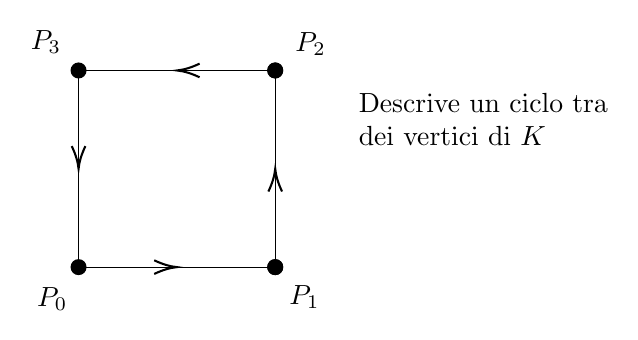
\begin{tikzpicture}[x=0.75pt,y=0.75pt,yscale=-1,xscale=1]
        %uncomment if require: \path (0,433); %set diagram left start at 0, and has height of 433

        %Shape: Square [id:dp311972140197708] 
        \draw   (162.75,39.75) -- (257.5,39.75) -- (257.5,134.5) -- (162.75,134.5) -- cycle ;
        %Straight Lines [id:da3375767366574549] 
        \draw    (162.75,39.75) -- (257.5,39.75) ;
        \draw [shift={(257.5,39.75)}, rotate = 0] [color={rgb, 255:red, 0; green, 0; blue, 0 }  ][fill={rgb, 255:red, 0; green, 0; blue, 0 }  ][line width=0.75]      (0, 0) circle [x radius= 3.35, y radius= 3.35]   ;
        \draw [shift={(162.75,39.75)}, rotate = 0] [color={rgb, 255:red, 0; green, 0; blue, 0 }  ][fill={rgb, 255:red, 0; green, 0; blue, 0 }  ][line width=0.75]      (0, 0) circle [x radius= 3.35, y radius= 3.35]   ;
        %Straight Lines [id:da9195953727513981] 
        \draw    (162.75,134.5) -- (257.5,134.5) ;
        \draw [shift={(257.5,134.5)}, rotate = 0] [color={rgb, 255:red, 0; green, 0; blue, 0 }  ][fill={rgb, 255:red, 0; green, 0; blue, 0 }  ][line width=0.75]      (0, 0) circle [x radius= 3.35, y radius= 3.35]   ;
        \draw [shift={(162.75,134.5)}, rotate = 0] [color={rgb, 255:red, 0; green, 0; blue, 0 }  ][fill={rgb, 255:red, 0; green, 0; blue, 0 }  ][line width=0.75]      (0, 0) circle [x radius= 3.35, y radius= 3.35]   ;
        %Straight Lines [id:da8059513303813619] 
        \draw    (162.75,134.5) -- (208.13,134.5) ;
        \draw [shift={(210.13,134.5)}, rotate = 180] [color={rgb, 255:red, 0; green, 0; blue, 0 }  ][line width=0.75]    (10.93,-3.29) .. controls (6.95,-1.4) and (3.31,-0.3) .. (0,0) .. controls (3.31,0.3) and (6.95,1.4) .. (10.93,3.29)   ;
        %Straight Lines [id:da2285831064146353] 
        \draw    (162.75,134.5) -- (162.75,39.75) ;
        %Straight Lines [id:da6732465533433227] 
        \draw    (162.75,39.75) -- (162.75,85.13) ;
        \draw [shift={(162.75,87.13)}, rotate = 270] [color={rgb, 255:red, 0; green, 0; blue, 0 }  ][line width=0.75]    (10.93,-3.29) .. controls (6.95,-1.4) and (3.31,-0.3) .. (0,0) .. controls (3.31,0.3) and (6.95,1.4) .. (10.93,3.29)   ;
        %Straight Lines [id:da06827916766160635] 
        \draw    (257.5,39.75) -- (212.13,39.75) ;
        \draw [shift={(210.13,39.75)}, rotate = 360] [color={rgb, 255:red, 0; green, 0; blue, 0 }  ][line width=0.75]    (10.93,-3.29) .. controls (6.95,-1.4) and (3.31,-0.3) .. (0,0) .. controls (3.31,0.3) and (6.95,1.4) .. (10.93,3.29)   ;
        %Straight Lines [id:da8480868265281654] 
        \draw    (257.5,39.75) -- (257.5,134.5) ;
        \draw [shift={(257.5,134.5)}, rotate = 90] [color={rgb, 255:red, 0; green, 0; blue, 0 }  ][fill={rgb, 255:red, 0; green, 0; blue, 0 }  ][line width=0.75]      (0, 0) circle [x radius= 3.35, y radius= 3.35]   ;
        \draw [shift={(257.5,39.75)}, rotate = 90] [color={rgb, 255:red, 0; green, 0; blue, 0 }  ][fill={rgb, 255:red, 0; green, 0; blue, 0 }  ][line width=0.75]      (0, 0) circle [x radius= 3.35, y radius= 3.35]   ;
        %Straight Lines [id:da8783982634233514] 
        \draw    (257.5,134.5) -- (257.5,89.13) ;
        \draw [shift={(257.5,87.13)}, rotate = 90] [color={rgb, 255:red, 0; green, 0; blue, 0 }  ][line width=0.75]    (10.93,-3.29) .. controls (6.95,-1.4) and (3.31,-0.3) .. (0,0) .. controls (3.31,0.3) and (6.95,1.4) .. (10.93,3.29)   ;

        % Text Node
        \draw (141.5,142.9) node [anchor=north west][inner sep=0.75pt]    {$P_{0}$};
        % Text Node
        \draw (263,141.9) node [anchor=north west][inner sep=0.75pt]    {$P_{1}$};
        % Text Node
        \draw (266,20.4) node [anchor=north west][inner sep=0.75pt]    {$P_{2}$};
        % Text Node
        \draw (138.5,19.4) node [anchor=north west][inner sep=0.75pt]    {$P_{3}$};
        % Text Node
        \draw (296.5,49.5) node [anchor=north west][inner sep=0.75pt]   [align=left] {Descrive un ciclo tra\\dei vertici di $\displaystyle K$};


    \end{tikzpicture}

\end{center}
\subsection{Conclusione}
Abbiamo quindi
\[
    H_p(K)=\left\{
    \begin{array}{ll}
        \Z    & p=0,1     \\
        \{0\} & p\neq 0,1
    \end{array}
    \right.
\]
\section{Esempio completo 2}
Calcolare i gruppi doi omologia simpliciale di
\begin{center}


    \tikzset{every picture/.style={line width=0.75pt}} %set default line width to 0.75pt        

    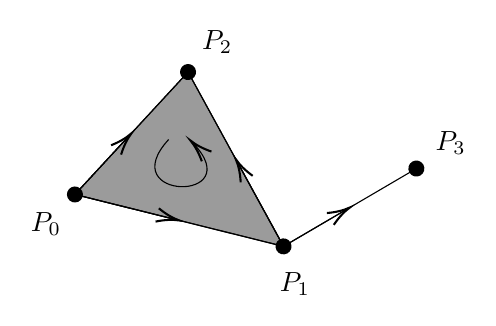
\begin{tikzpicture}[x=0.75pt,y=0.75pt,yscale=-1,xscale=1]
        %uncomment if require: \path (0,433); %set diagram left start at 0, and has height of 433

        %Shape: Polygon [id:ds934146185035563] 
        \draw  [fill={rgb, 255:red, 155; green, 155; blue, 155 }  ,fill opacity=1 ] (148.5,27.5) -- (194.5,111.5) -- (94,86.5) -- (94,86.5) -- (94,86.5) -- cycle ;
        %Straight Lines [id:da12202989709972001] 
        \draw    (148.5,27.5) -- (194.5,111.5) ;
        \draw [shift={(194.5,111.5)}, rotate = 61.29] [color={rgb, 255:red, 0; green, 0; blue, 0 }  ][fill={rgb, 255:red, 0; green, 0; blue, 0 }  ][line width=0.75]      (0, 0) circle [x radius= 3.35, y radius= 3.35]   ;
        \draw [shift={(148.5,27.5)}, rotate = 61.29] [color={rgb, 255:red, 0; green, 0; blue, 0 }  ][fill={rgb, 255:red, 0; green, 0; blue, 0 }  ][line width=0.75]      (0, 0) circle [x radius= 3.35, y radius= 3.35]   ;
        %Straight Lines [id:da8090863506577006] 
        \draw    (194.5,111.5) -- (258.5,74) ;
        \draw [shift={(258.5,74)}, rotate = 329.63] [color={rgb, 255:red, 0; green, 0; blue, 0 }  ][fill={rgb, 255:red, 0; green, 0; blue, 0 }  ][line width=0.75]      (0, 0) circle [x radius= 3.35, y radius= 3.35]   ;
        %Straight Lines [id:da30985777948192217] 
        \draw    (94,86.5) -- (148.5,27.5) ;
        \draw [shift={(94,86.5)}, rotate = 312.73] [color={rgb, 255:red, 0; green, 0; blue, 0 }  ][fill={rgb, 255:red, 0; green, 0; blue, 0 }  ][line width=0.75]      (0, 0) circle [x radius= 3.35, y radius= 3.35]   ;
        %Straight Lines [id:da2361933770040765] 
        \draw    (94,86.5) -- (194.5,111.5) ;
        %Shape: Boxed Bezier Curve [id:dp24035206760234518] 
        \draw    (139.16,60) .. controls (112.07,89.55) and (178.13,90.48) .. (150.97,61.83) ;
        \draw [shift={(149.66,60.5)}, rotate = 44.53] [color={rgb, 255:red, 0; green, 0; blue, 0 }  ][line width=0.75]    (10.93,-3.29) .. controls (6.95,-1.4) and (3.31,-0.3) .. (0,0) .. controls (3.31,0.3) and (6.95,1.4) .. (10.93,3.29)   ;
        %Straight Lines [id:da2682069712809334] 
        \draw    (94,86.5) -- (142.31,98.52) ;
        \draw [shift={(144.25,99)}, rotate = 193.97] [color={rgb, 255:red, 0; green, 0; blue, 0 }  ][line width=0.75]    (10.93,-3.29) .. controls (6.95,-1.4) and (3.31,-0.3) .. (0,0) .. controls (3.31,0.3) and (6.95,1.4) .. (10.93,3.29)   ;
        %Straight Lines [id:da1792608347016602] 
        \draw    (94,86.5) -- (119.89,58.47) ;
        \draw [shift={(121.25,57)}, rotate = 132.73] [color={rgb, 255:red, 0; green, 0; blue, 0 }  ][line width=0.75]    (10.93,-3.29) .. controls (6.95,-1.4) and (3.31,-0.3) .. (0,0) .. controls (3.31,0.3) and (6.95,1.4) .. (10.93,3.29)   ;
        %Straight Lines [id:da8870416584805199] 
        \draw    (194.5,111.5) -- (224.77,93.76) ;
        \draw [shift={(226.5,92.75)}, rotate = 149.63] [color={rgb, 255:red, 0; green, 0; blue, 0 }  ][line width=0.75]    (10.93,-3.29) .. controls (6.95,-1.4) and (3.31,-0.3) .. (0,0) .. controls (3.31,0.3) and (6.95,1.4) .. (10.93,3.29)   ;
        %Straight Lines [id:da6774740222674873] 
        \draw    (194.5,111.5) -- (172.46,71.25) ;
        \draw [shift={(171.5,69.5)}, rotate = 61.29] [color={rgb, 255:red, 0; green, 0; blue, 0 }  ][line width=0.75]    (10.93,-3.29) .. controls (6.95,-1.4) and (3.31,-0.3) .. (0,0) .. controls (3.31,0.3) and (6.95,1.4) .. (10.93,3.29)   ;

        % Text Node
        \draw (71.5,93.9) node [anchor=north west][inner sep=0.75pt]    {$P_{0}$};
        % Text Node
        \draw (191.5,122.9) node [anchor=north west][inner sep=0.75pt]    {$P_{1}$};
        % Text Node
        \draw (154,6.4) node [anchor=north west][inner sep=0.75pt]    {$P_{2}$};
        % Text Node
        \draw (266.5,54.9) node [anchor=north west][inner sep=0.75pt]    {$P_{3}$};


    \end{tikzpicture}

\end{center}
\[
    H_0(K)=\faktor{Z_0(K)}{B_0(K)}=\faktor{C_0(K)}{B_0(K)}
\]
\[
    H_1(K)=\faktor{Z_1(K)}{B_1(K)}=\faktor{Ker\ \partial_1}{Im\ \partial_2}
\]
\[
    H_2(K)=\faktor{Z_2(K)}{B_2(K)}=\faktor{Ker\ \partial_2}{Im\ \partial_3}=Ker\ \partial_2
\]
\subsection{$H_0(K)$}
$Im\ \partial_2$ è generato dalle immagini degli elementi della base di $C_2(K)$, ossia
\[
    P_1-P_0\quad P_2-P_1\quad P_2-P_0\quad P_3-P_1
\]
E' immediato verificare che
\[
    1(P_1-P_0)+1(P_2-P_3)-1(P_2-P_0)+0(P_3-P_1)=0
\]
ossia
\[
    B_0(K)=\gen{P_1-P_0,P_2-P_3,P_3-P_1}\simeq\Z^3
\]
\[
    H_0(K)=\faktor{C_0(K)}{B_0(K)}\simeq\Z
\]
\subsection{$H_2(K)$}
\[
    \partial_2=\begin{bmatrix}
        1 \\1\\-1\\0
    \end{bmatrix}
\]
ossia
\[
    a[P_0,P_1,P_2]\overset{\partial_2}{\longmapsto}a([P_0,P_1]+[P_1,P_2]-[P_0,P_2])
\]
\[
    a[P_0,P_1,P_2]\in Ker\ \partial_2\Longleftrightarrow a=0\implies Ker\ \partial_2=\{0\}
\]
da cui
\[
    H_2(K)=\{0\}
\]
\subsection{$H_1(K)$}
\[
    H_1(K)=\faktor{Ker\ \partial_1}{Im\ \partial_2}
\]
è facile verificare che
\[
    Ker\ \partial_1=\gen{[P_0,P_1]+[P_1,P_2]-[P_0,P_2]}\simeq\Z
\]
Inoltre, $Im\ \partial_2$ è generato dall'immagine della base di $C_2(K)$
\[
    \partial_2[P_0,P_1,P_2]=[P_0,P_1]+[P_1,P_2]-[P_0,P_2]
\]
\[
    Im\ \partial_2=\gen{[P_0,P_1]+[P_1,P_2]-[P_0,P_3]}\simeq Z\simeq Ker\ \partial_1
\]
da cui
\[
    H_1(K)=\{0\}
\]
\subsection{Conclusione}
Abbiamo quindi
\[
    H_p(K)=\left\{
    \begin{array}{ll}
        \Z    & p=0     \\
        \{0\} & p\neq 0
    \end{array}
    \right.
\]
\subsection{Interpretazione topologica}
\paragraph{Osservazione} Il gruppo di omologia $H_0(K)$ ha una interpretazione molto utile, riassumibile nel seguente teorema
\begin{theorem}
    Sia $K$ un complesso simpliciale, allora
    \begin{enumerate}
        \item Il gruppo $H_0(K)$ è un gruppo libero
        \item Sia $\{P_\alpha\}$ una collezione di vertici di $K$ ($\subseteq\pskel{K}{0}$) tali che he no uno per ogni componente connessa di $|K|$. Allora le classi di omologia delle funzioni caratteristiche dei punti selezionati formano una base dello 0-esimo gruppo di omologia
    \end{enumerate}
\end{theorem}
\paragraph{In poche parole} Il rango di $H_0(K)$ ci dice il numero di componenti connesse di $|K|$
\begin{proof}
    \begin{enumerate}
        \item[2.] Definisco la seguente relazioen di equivalenza tra i vertici di $K$:\\
            $P\sim Q$ se e solo se esiste una sequenza di vertici $P_0,P_1,\dots,P_n$ tali che $P_0=P$, $P_n=Q$ e $\{P_{i-1},P_i\}$ sia un 1-simplesso di $K$ per ogni $i$ (scriviamo $\{P_{i-1},P_i\}$ invece di $[P_{i-1},P_i]$ per indicare l'1-simplesso privo di orientazione)\\
            Per ogni vertice $P\in\pskel{K}{0}$, definisco
            \[
                C_P=\bigcup_{Q\sim P}St(Q)\subseteq |K|
            \]
            Voglio far vedere che gli insiemi $C_P$ (al variare della classe di equivalenza) descrivono le componenti connesse di $|K|$\\
            \textbf{Osservazioni}
            \begin{enumerate}
                \item $C_P$ è un sottoinsieme aperto di $|K|$, poichè unione di aperti
                \item $P\sim Q\implies C_P=C_Q$
                \item $C_P$ è un insieme connesso (per archi), infatti, se prendo $P\sim Q$ e $x\in St(Q)$, per definizione della relazione di equivalenza, esiste una successione
                      \[
                          P=P_0,P_1,\dots,P_n=Q\quad {P_{i-1},P_i}\in K\ \text{1-simplessi}
                      \]
                      La spezzata di vertici $P_0,P_1,\dots,P_n,x$ appartiene a $C_P$, infatti
                      \[
                          P_i\sim P\implies St(P_i)\subset C_P
                      \]
                      in particolare
                      \[
                          \{P_i,P_{i+1}\}\subseteq\overline{St(P_i)}\subseteq C_P
                      \]
                      Inoltre
                      \[
                          \{P_n,x\}\subseteq\overline{St(P_n)}\subseteq C_P
                      \]
                      Mettendo tutto insieme ho mostrato che un qualsiasi punto $x\in St(Q)$ con $Q\sim P$ è collegato a $P$ tramite una spezzata contenuta in $C_P$
                \item Voglio far vedere che $P\nsim Q$ implica che $C_P\cap C_Q=\emptyset$\\
                      Supponiamo che ci sia un $x\in C_P\cap C_Q$
                      \[
                          x\in C_P\cap C_Q\implies\begin{cases}
                              x\in C_P\implies x\in St(P')\ \text{con }P'\sim P \\
                              x\in C_Q\implies x\in St(Q')\ \text{con }Q'\sim Q \\
                          \end{cases}
                      \]
                      $x$ deve quindi appartenere ad un simplesso $\sigma$ che ha $P'$ e $Q'$ tra i suoi vertici, ossia $\{P',Q'\}$ è una faccia del simplesso $\sigma$. Quindi $P'\sim Q'$, ma allora
                      \[
                          P\sim P'\sim Q'\sim Q\implies P\sim Q\implies C_P=C_Q
                      \]
                      Quindi $\{C_P\}$ sono insiemi aperti, connessi, e a due a due disgiunti, ossia $\{C_P\}$ sono le componenti connesse di $|K|$
            \end{enumerate}
        \item[1.] Sia $\{P_\alpha\}$ una collezione di vertici, presi uno per ogni componente connessa di $|K|$. Inizio mostrando che le classi di omologia di $\{P_\alpha\}$ formano un insieme di generatori di $H_0(K)$.\\
            Per ogni $Q\in\pskel{K}{0}$, esiste un unico $P_\alpha$ tale che $Q\sim P_\alpha$, cioè $Q\in C_{P_\alpha}$, quindi esiste una successione di vertici di $K$ tali che
            \[
                P_\alpha=P_0,P_1,\dots,P_n=Q\quad \{P_{i+1},P_i\}\in K
            \]
            Considero la 1-catena che descrive il cammino da $P_\alpha$ a $Q$
            \[
                \sigma=[P_\alpha,P_1]+[P_1,P_2]+\dots+[P_{n-1},Q]
            \]
            \[
                \partial_1\sigma=Q-P_\alpha
            \]
            da cui segue
            \[
                H_0(K)=\faktor{Z_0(K)}{B_0(K)}=\faktor{C_0(K)}{Im\ \partial_1}
            \]
            \[
                Q-P_\alpha\in B_0(K)\implies [Q-P_\alpha]=0\text{ in }H_0(K)
            \]
            quindi
            \[
                [Q]=[P_\alpha]\implies \{[P_\alpha]\}\text{ generatore di }H_0(K)
            \]
            Rimane da far vedere che non ci sono relazioni tra le classi $\{[P_\alpha]\}$\\
            Sia
            \[
                c=\sum n_\alpha P_\alpha\in C_0(K)
            \]
            e supponiamo che $c=\partial_1\sigma$ per qualche $\sigma\in C_1(K)$, ossia
            \[
                c\in Im\ \partial_1\implies c\in B_0(K)\implies [c]=0_{H_0(K)}
            \]
            Ogni 1-simplessso può appartenere a una sola componente connessa, quindi decompongo $\sigma$ secondo le componenti connesse di $|K|$
            \[
                \sigma=\sum\sigma_\alpha
            \]
            dove $\sigma_\alpha$ coinvolge 1-simplessi nella componente connessa corrispondente $C_{P_\alpha}$
            \[
                \partial_1\sigma=\sum\partial_1\sigma_\alpha
            \]
            ossia $\partial_1\sigma_\alpha$ è una 0-catena che coinvilge 0-simplessi (vertici) appartenenti a $C_{P_\alpha}$
            \[
                c=\partial_1 d\Longleftrightarrow\partial_1\sigma_\alpha=n_\alpha P_\alpha\quad \forall\alpha
            \]
            ossia
            \[
                c\in B_0(K)
            \]
            quindi l'unica possibilità è $n\alpha=0$\\
            "L'unico modo che ho per costruire un bordo a partire dai vertici $\{P_\alpha\}$ delle componenti connesse di $|K|$ è considerare la 0-catena con tutti i coefficenti nulli"
    \end{enumerate}
\end{proof}
\section{Gruppo di omologia ridotta}
\begin{definition}[Augmentation map]
    Sia $K$ un complesso simpliciale, definisco l'omomorfismo
    \[
        \varepsilon:C_0(K)\ra\Z
    \]
    come l'omomorfismo
    \[
        P\longmapsto 1\quad \forall P\in C_0(K)
    \]
    e lo chiamerò augmentation map di $C_0(K)$, e per ogni
    \[
        \sum n_jP_j\in C_0(K)
    \]
    abbiamo
    \[
        \varepsilon\left(\sum n_jP_j\right)=\sum n_j\varepsilon(P_j)=\sum n_j
    \]
\end{definition}
Lo scopo dell'augmentation map è quella di allungare la successione di gruppi e omomorfismi di omologia simpliciale, infatti da
\[\begin{tikzcd}
        \dots && {C_1(K)} && {C_0(K)} && {\{0\}}
        \arrow["{\partial_2}", from=1-1, to=1-3]
        \arrow["{\partial_1}", from=1-3, to=1-5]
        \arrow["{\partial_0}", from=1-5, to=1-7]
    \end{tikzcd}\]
passiamo a
\[\begin{tikzcd}
        \dots && {C_1(K)} && {C_0(K)} && \Z && {\{0\}}
        \arrow["{\partial_2}", from=1-1, to=1-3]
        \arrow["{\partial_1}", from=1-3, to=1-5]
        \arrow["\varepsilon", from=1-5, to=1-7]
        \arrow[from=1-7, to=1-9]
    \end{tikzcd}\]
\begin{proposition}
    \[
        \forall\sigma\in C_1(K)\quad \varepsilon(\partial_1\sigma)=0
    \]
\end{proposition}
\begin{proof}
    Verifico che $\varepsilon(\partial_1\sigma)=0$ per $\sigma$ elemento della base di $C_1(K)$
    \[
        \sigma=[P,Q]
    \]
    \[
        \partial_1[P,Q]=Q-P
    \]
    \[
        \varepsilon(\partial_1\sigma)=\varepsilon(Q-P)=\varepsilon(Q)-\varepsilon(P)=1-1=0
    \]
\end{proof}
\paragraph{Osservazione} Otteniamo quindi che
\[
    \varepsilon\circ\partial_1=0\implies Im\ \partial_1\subseteq Ker\ \varepsilon
\]
Possiamo quindi definire un nuovo gruppo
\begin{definition}[Gruppo di omologia simpliciale ridotta]
    Dato un complesso simpliciale $K$, definiamo gruppo di omologia ridotta di $K$ di dimensione 0 il gruppo quoziente
    \[
        \tilde{H_0}(K):=\faktor{Ker\ \varepsilon}{Im\ \partial_1}
    \]
\end{definition}
\paragraph{Osservazione} Dalla definizione, risulta che
\[
    \forall p>0\quad \tilde{H_p}(K)=H_p(K)
\]
\chapter{Metodo di calcolo dei gruppi di omologia simpliciale}
Siamo ora interessati a trovare un metodo algebrico efficace per il calcolo dei gruppi di omologia simpliciale
\begin{theorem}[Forma normale di Smith]
    Sia $f:\Z^n\ra\Z^m$ un omomorfismo di gruppi liberi. Esistono due basi $\mathcal{B}$ di $\Z^n$ e $\mathcal{C}$ di $\Z^m$ tali che la matrice rappresentativa di $f$ rispetto a $\mathcal{B}$ e $\mathcal{C}$ è della forma
    \[
        A=\left[\begin{array}{@{}c|c@{}}
                \begin{matrix}
                    a_{11} & 0      & \dots  & 0      \\
                    0      & a_{22} & \dots  & 0      \\
                    \vdots & \vdots & \ddots & \vdots \\
                    0      & 0      & \dots  & a_{nn}
                \end{matrix}
                  & 0 \\
                \hline
                0 & 0
            \end{array}\right]
    \]
    dove
    \[
        a_{11}|a_{22}|\dots|a_{nn}\quad\quad a_{ii}\in\Z_{>0}
    \]
\end{theorem}
\paragraph{Calcolo della forma di Smith} Per il calcolo della forma di Smith, si procede in modo simile al metodo di eliminazione di Gauss.\\
Le operazioni consentite sono:
\begin{itemize}
    \item Scambi di righe o colonne
          \[
              C_i\longleftrightarrow C_j\quad\quad R_i\longleftrightarrow R_j
          \]
    \item Cambio di segno di righe o colonne
          \[
              -C_i\longrightarrow C_i\quad\quad -R_i\longrightarrow R_i
          \]
    \item Somma di una righa o una colonna con il multiplo di un'altra
          \[
              C_i+qC_j\longrightarrow C_i\quad\quad R_i+qR_j\longrightarrow R_i
          \]
          con $q\in\Z$
\end{itemize}
\section{Esempio}
\begin{center}


    \tikzset{every picture/.style={line width=0.75pt}} %set default line width to 0.75pt        

    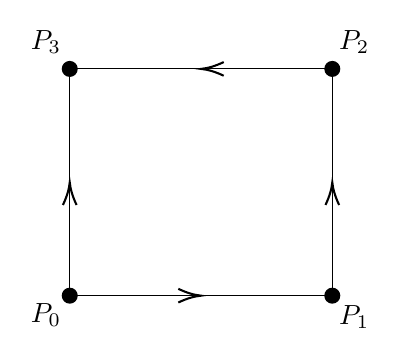
\begin{tikzpicture}[x=0.75pt,y=0.75pt,yscale=-1,xscale=1]
        %uncomment if require: \path (0,735); %set diagram left start at 0, and has height of 735

        %Straight Lines [id:da24826936228573415] 
        \draw    (112,61.5) -- (238.5,61.5) ;
        \draw [shift={(238.5,61.5)}, rotate = 0] [color={rgb, 255:red, 0; green, 0; blue, 0 }  ][fill={rgb, 255:red, 0; green, 0; blue, 0 }  ][line width=0.75]      (0, 0) circle [x radius= 3.35, y radius= 3.35]   ;
        \draw [shift={(112,61.5)}, rotate = 0] [color={rgb, 255:red, 0; green, 0; blue, 0 }  ][fill={rgb, 255:red, 0; green, 0; blue, 0 }  ][line width=0.75]      (0, 0) circle [x radius= 3.35, y radius= 3.35]   ;
        %Straight Lines [id:da8776917918483467] 
        \draw    (238.5,61.5) -- (238.5,170.75) ;
        %Straight Lines [id:da6285692892561223] 
        \draw    (112,170.75) -- (238.5,170.75) ;
        \draw [shift={(238.5,170.75)}, rotate = 0] [color={rgb, 255:red, 0; green, 0; blue, 0 }  ][fill={rgb, 255:red, 0; green, 0; blue, 0 }  ][line width=0.75]      (0, 0) circle [x radius= 3.35, y radius= 3.35]   ;
        \draw [shift={(112,170.75)}, rotate = 0] [color={rgb, 255:red, 0; green, 0; blue, 0 }  ][fill={rgb, 255:red, 0; green, 0; blue, 0 }  ][line width=0.75]      (0, 0) circle [x radius= 3.35, y radius= 3.35]   ;
        %Straight Lines [id:da9801759631021449] 
        \draw    (112,61.5) -- (112,170.75) ;
        %Straight Lines [id:da8936345955185903] 
        \draw    (238.5,61.5) -- (177.25,61.5) ;
        \draw [shift={(175.25,61.5)}, rotate = 360] [color={rgb, 255:red, 0; green, 0; blue, 0 }  ][line width=0.75]    (10.93,-3.29) .. controls (6.95,-1.4) and (3.31,-0.3) .. (0,0) .. controls (3.31,0.3) and (6.95,1.4) .. (10.93,3.29)   ;
        %Straight Lines [id:da5484737152200554] 
        \draw    (112,170.75) -- (112,118.13) ;
        \draw [shift={(112,116.13)}, rotate = 90] [color={rgb, 255:red, 0; green, 0; blue, 0 }  ][line width=0.75]    (10.93,-3.29) .. controls (6.95,-1.4) and (3.31,-0.3) .. (0,0) .. controls (3.31,0.3) and (6.95,1.4) .. (10.93,3.29)   ;
        %Straight Lines [id:da13143294691324892] 
        \draw    (238.5,170.75) -- (238.5,118.13) ;
        \draw [shift={(238.5,116.13)}, rotate = 90] [color={rgb, 255:red, 0; green, 0; blue, 0 }  ][line width=0.75]    (10.93,-3.29) .. controls (6.95,-1.4) and (3.31,-0.3) .. (0,0) .. controls (3.31,0.3) and (6.95,1.4) .. (10.93,3.29)   ;
        %Straight Lines [id:da9546977398566023] 
        \draw    (112,170.75) -- (173.25,170.75) ;
        \draw [shift={(175.25,170.75)}, rotate = 180] [color={rgb, 255:red, 0; green, 0; blue, 0 }  ][line width=0.75]    (10.93,-3.29) .. controls (6.95,-1.4) and (3.31,-0.3) .. (0,0) .. controls (3.31,0.3) and (6.95,1.4) .. (10.93,3.29)   ;

        % Text Node
        \draw (92,173.4) node [anchor=north west][inner sep=0.75pt]    {$P_{0}$};
        % Text Node
        \draw (240.5,174.15) node [anchor=north west][inner sep=0.75pt]    {$P_{1}$};
        % Text Node
        \draw (240.5,41.9) node [anchor=north west][inner sep=0.75pt]    {$P_{2}$};
        % Text Node
        \draw (92,41.9) node [anchor=north west][inner sep=0.75pt]    {$P_{3}$};


    \end{tikzpicture}

\end{center}
\[
    \partial_1=\begin{blockarray}{rrrrl}
        [P_0,P_1] & [P_1,P_2] & [P_2,P_3] & [P_0,P_3] & \\
        \begin{block}{[cccc]l}
            -1 & 0 & 0 & -1\topstrut & P_0 \\
            1 & -1 & 0 & 0 & P_1 \\
            0 & 1 & -1 & 0 & P_2 \\
            0 & 0 & 1 & 1\botstrut & P_3 \\
        \end{block}
    \end{blockarray}
\]
$R_1\longleftrightarrow R_2$
\[
    \partial_1=\begin{blockarray}{rrrrl}
        [P_0,P_1] & [P_1,P_2] & [P_2,P_3] & [P_0,P_3] & \\
        \begin{block}{[cccc]l}
            1 & -1 & 0 & 0\topstrut & P_1 \\
            -1 & 0 & 0 & -1 & P_0 \\
            0 & 1 & -1 & 0 & P_2 \\
            0 & 0 & 1 & 1\botstrut & P_3 \\
        \end{block}
    \end{blockarray}
\]
$R_2+R_1\longrightarrow R_2$
\[
    \partial_1=\begin{blockarray}{rrrrl}
        [P_0,P_1] & [P_1,P_2] & [P_2,P_3] & [P_0,P_3] & \\
        \begin{block}{[cccc]l}
            1 & -1 & 0 & 0\topstrut & P_1 \\
            0 & -1 & 0 & -1 & P_0+P_1 \\
            0 & 1 & -1 & 0 & P_2 \\
            0 & 0 & 1 & 1\botstrut & P_3 \\
        \end{block}
    \end{blockarray}
\]
$R_2\longleftrightarrow R_3$
\[
    \partial_1=\begin{blockarray}{rrrrl}
        [P_0,P_1] & [P_1,P_2] & [P_2,P_3] & [P_0,P_3] & \\
        \begin{block}{[cccc]l}
            1 & -1 & 0 & 0\topstrut & P_1 \\
            0 & 1 & -1 & 0 & P_2 \\
            0 & -1 & 0 & -1 & P_0+P_1 \\
            0 & 0 & 1 & 1\botstrut & P_3 \\
        \end{block}
    \end{blockarray}
\]
$R_3+R_2\longrightarrow R_3$
\[
    \partial_1=\begin{blockarray}{rrrrl}
        [P_0,P_1] & [P_1,P_2] & [P_2,P_3] & [P_0,P_3] & \\
        \begin{block}{[cccc]l}
            1 & -1 & 0 & 0\topstrut & P_1 \\
            0 & 1 & -1 & 0 & P_2 \\
            0 & 0 & -1 & -1 & P_0+P_1+P_2 \\
            0 & 0 & 1 & 1\botstrut & P_3 \\
        \end{block}
    \end{blockarray}
\]
$R_3\longleftrightarrow R_4$
\[
    \partial_1=\begin{blockarray}{rrrrl}
        [P_0,P_1] & [P_1,P_2] & [P_2,P_3] & [P_0,P_3] & \\
        \begin{block}{[cccc]l}
            1 & -1 & 0 & 0\topstrut & P_1 \\
            0 & 1 & -1 & 0 & P_2 \\
            0 & 0 & 1 & 1 & P_3 \\
            0 & 0 & -1 & -1\botstrut & P_0+P_1+P_2 \\
        \end{block}
    \end{blockarray}
\]
$R_4+R_3\longrightarrow R_4$
\[
    \partial_1=\begin{blockarray}{rrrrl}
        [P_0,P_1] & [P_1,P_2] & [P_2,P_3] & [P_0,P_3] & \\
        \begin{block}{[cccc]l}
            1 & -1 & 0 & 0\topstrut & P_1 \\
            0 & 1 & -1 & 0 & P_2 \\
            0 & 0 & 1 & 1 & P_3 \\
            0 & 0 & 0 & 0\botstrut & P_0+P_1+P_2+P_3 \\
        \end{block}
    \end{blockarray}
\]
$C_2+C_1\longrightarrow C_2$
\[
    \partial_1=\begin{blockarray}{rrrrl}
        [P_0,P_1] & [P_1,P_2] & [P_2,P_3] & [P_0,P_3] & \\
        & +[P_0,P_1] & & &\\
        \begin{block}{[cccc]l}
            1 & 0 & 0 & 0\topstrut & P_1 \\
            0 & 1 & -1 & 0 & P_2 \\
            0 & 0 & 1 & 1 & P_3 \\
            0 & 0 & 0 & 0\botstrut & P_0+P_1+P_2+P_3 \\
        \end{block}
    \end{blockarray}
\]
$C_3+C_2\longrightarrow C_3$
\[
    \partial_1=\begin{blockarray}{rrrrl}
        [P_0,P_1] & [P_0,P_1] & [P_0,P_1] & [P_0,P_3] & \\
        & +[P_1,P_2] & +[P_1,P_2] & &\\
        & & +[P_2,P_3] & &\\
        \begin{block}{[cccc]l}
            1 & 0 & 0 & 0\topstrut & P_1 \\
            0 & 1 & 0 & 0 & P_2 \\
            0 & 0 & 1 & 1 & P_3 \\
            0 & 0 & 0 & 0\botstrut & P_0+P_1+P_2+P_3 \\
        \end{block}
    \end{blockarray}
\]
$C_4-C_3\longrightarrow C_4$
\[
    \partial_1=\begin{blockarray}{rrrrl}
        [P_0,P_1] & [P_0,P_1] & [P_0,P_1] & [P_0,P_3] & \\
        & +[P_1,P_2] & +[P_1,P_2] & -[P_0,P_1]&\\
        & & +[P_2,P_3] & -[P_1,P_2]&\\
        & & & -[P_2,P_3] & \\
        \begin{block}{[cccc]l}
            1 & 0 & 0 & 0\topstrut & P_1 \\
            0 & 1 & 0 & 0 & P_2 \\
            0 & 0 & 1 & 0 & P_3 \\
            0 & 0 & 0 & 0\botstrut & P_0+P_1+P_2+P_3 \\
        \end{block}
    \end{blockarray}
\]
\[
    \partial_1:C_1(K)\ra C_0(K)
\]
ossia, dalla matrice
\[
    \gen{[P_0,P_1],\dots,[P_0,P_3]-[P_0,P_1]-[P_1,P_2]-[P_2,P_3]}\ra\gen{P_1,P_2,P_3,P_0+P_1+P_2+P_3}
\]
\[
    H_1(K)=Z_1(K)=Ker\ \partial_1=\gen{[P_0,P_3]-[P_0,P_1]-[P_1,P_2]-[P_2,P_3]}\simeq \Z
\]
(guardo le colonne con entrate tutte nulle)
\[
    H_0(K)=\faktor{C_0(K)}{Im\ \partial_1}=\faktor{\gen{\cancel{P_1},\cancel{P_2},\cancel{P_3},P_0+P_1+P_2+P_3}}{\gen{\cancel{P_1},\cancel{P_2},\cancel{P_3}}}\simeq
\]
\[
    \simeq\gen{P_0+P_1+P_2+P_3}
\]
notiamo come $P_1+P_2+P_3$ è l'elemento che genera il gruppo per cui quozientiamo, da cui segue
\[
    [P_0+P_1+P_2+P_3]_{\gen{P_1,P_2,P_3}}=[P_0]_{\gen{P_1,P_2,P_3}}\implies\gen{P_0+P_1+P_2+P_3}\simeq\gen{P_0}\simeq\Z
\]
\pagebreak
\section{Esempio particolare - Nastro di Möbius}
Prendo una striscia di carta ed eseguo la seguente costruzione
\begin{center}


    \tikzset{every picture/.style={line width=0.75pt}} %set default line width to 0.75pt        

    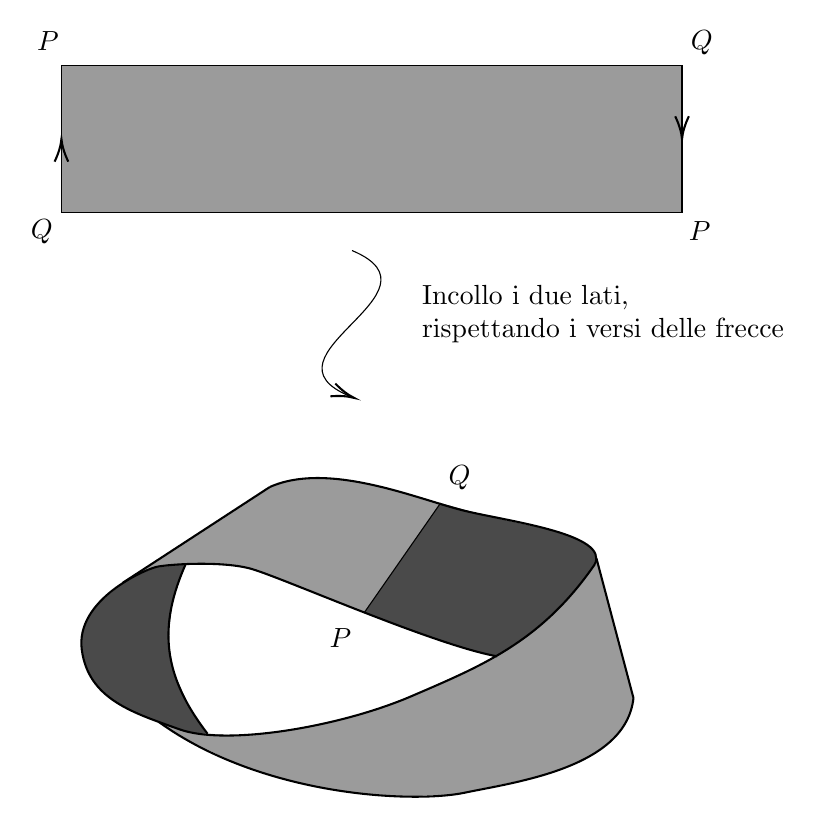
\begin{tikzpicture}[x=0.75pt,y=0.75pt,yscale=-1,xscale=1]
        %uncomment if require: \path (0,735); %set diagram left start at 0, and has height of 735

        %Shape: Polygon [id:ds23564581044041844] 
        \draw  [draw opacity=0][fill={rgb, 255:red, 155; green, 155; blue, 155 }  ,fill opacity=1 ] (307.8,297.4) -- (325.6,364.6) -- (322.83,375.5) -- (314.83,385.5) -- (301.83,394.17) -- (281.5,402.17) -- (238.17,411.17) -- (215.33,412) -- (188,410) -- (158,404) -- (134,396) -- (109,384) -- (97,376.2) -- (120.4,381.8) -- (137.33,382.67) -- (158.33,380.5) -- (193.33,372.83) -- (221.67,362.5) -- (260,344.53) -- cycle ;
        %Shape: Polygon [id:ds8630216728697748] 
        \draw  [draw opacity=0][fill={rgb, 255:red, 74; green, 74; blue, 74 }  ,fill opacity=1 ] (96.2,301.33) -- (110,299.8) -- (103.67,317.17) -- (101.33,335.83) -- (104,351.83) -- (111.67,369.17) -- (120.4,381.8) -- (112.17,381.17) -- (97,376.2) -- (83.17,370.67) -- (73.5,364.67) -- (65.83,357.5) -- (60.83,347.33) -- (59.5,337.67) -- (61.17,328.83) -- (67.17,319.5) -- (79.67,309) -- (87,305.17) -- cycle ;
        %Shape: Polygon [id:ds4077467238818855] 
        \draw  [draw opacity=0][fill={rgb, 255:red, 74; green, 74; blue, 74 }  ,fill opacity=1 ] (232.67,270.67) -- (196,323.33) -- (227,335) -- (248.33,341.67) -- (260,344.53) -- (272.33,336.33) -- (284.33,326.5) -- (296,314.17) -- (306,301.5) -- (307.8,297.4) -- (305.67,292.5) -- (298.33,288) -- (284.33,283.33) -- (256.67,277.33) -- cycle ;
        %Straight Lines [id:da14555538680601154] 
        \draw [draw opacity=0][fill={rgb, 255:red, 155; green, 155; blue, 155 }  ,fill opacity=1 ]   (163.83,311) -- (143.67,303.17) -- (133,300.83) -- (110,299.8) -- (92.67,302.17) -- (79.67,309) -- (150.4,262.93) -- (156.5,260.33) -- (170.17,258.67) -- (185.17,259.33) -- (204.33,262.67) -- (232.67,270.67) -- (196,323.33) ;
        %Shape: Rectangle [id:dp5300142836308106] 
        \draw  [fill={rgb, 255:red, 155; green, 155; blue, 155 }  ,fill opacity=1 ] (50,60) -- (349,60) -- (349,130.5) -- (50,130.5) -- cycle ;
        %Straight Lines [id:da6922579025607085] 
        \draw    (50,130.5) -- (50,60) ;
        %Straight Lines [id:da7283454077475491] 
        \draw    (349,130.5) -- (349,60) ;
        %Straight Lines [id:da7315695543071055] 
        \draw    (50,130.5) -- (50,97.25) ;
        \draw [shift={(50,95.25)}, rotate = 90] [color={rgb, 255:red, 0; green, 0; blue, 0 }  ][line width=0.75]    (10.93,-3.29) .. controls (6.95,-1.4) and (3.31,-0.3) .. (0,0) .. controls (3.31,0.3) and (6.95,1.4) .. (10.93,3.29)   ;
        %Straight Lines [id:da48061354232886555] 
        \draw    (349,60) -- (349,93.25) ;
        \draw [shift={(349,95.25)}, rotate = 270] [color={rgb, 255:red, 0; green, 0; blue, 0 }  ][line width=0.75]    (10.93,-3.29) .. controls (6.95,-1.4) and (3.31,-0.3) .. (0,0) .. controls (3.31,0.3) and (6.95,1.4) .. (10.93,3.29)   ;
        %Curve Lines [id:da6556345996581576] 
        \draw    (190,149) .. controls (238.51,169.3) and (140.99,199.88) .. (189.49,219.41) ;
        \draw [shift={(191,220)}, rotate = 200.56] [color={rgb, 255:red, 0; green, 0; blue, 0 }  ][line width=0.75]    (10.93,-3.29) .. controls (6.95,-1.4) and (3.31,-0.3) .. (0,0) .. controls (3.31,0.3) and (6.95,1.4) .. (10.93,3.29)   ;
        %Curve Lines [id:da6475253012208209] 
        \draw [color={rgb, 255:red, 0; green, 0; blue, 0 }  ,draw opacity=1 ][line width=0.75]    (307,300.13) .. controls (281.4,337.33) and (253,348.93) .. (218.6,363.73) .. controls (184.2,378.53) and (129.4,387.73) .. (107,379.73) .. controls (84.6,371.73) and (63,365.33) .. (59.8,341.33) .. controls (56.6,317.33) and (90.2,302.53) .. (96.2,301.33) .. controls (102.2,300.13) and (126.6,298.53) .. (140.6,302.13) .. controls (154.6,305.73) and (228.8,338.93) .. (260,344.53) ;
        %Straight Lines [id:da9891827109518274] 
        \draw [color={rgb, 255:red, 0; green, 0; blue, 0 }  ,draw opacity=1 ][line width=0.75]    (307.8,297.4) -- (325.6,364.6) ;
        %Straight Lines [id:da429480577377944] 
        \draw [color={rgb, 255:red, 0; green, 0; blue, 0 }  ,draw opacity=1 ][line width=0.75]    (79.67,309) -- (150.4,262.93) ;
        %Curve Lines [id:da7399803612615179] 
        \draw [color={rgb, 255:red, 0; green, 0; blue, 0 }  ,draw opacity=1 ][line width=0.75]    (110,299.8) .. controls (96.4,330.2) and (98.8,353.8) .. (120.4,381.8) ;
        %Curve Lines [id:da5893013804474581] 
        \draw [color={rgb, 255:red, 0; green, 0; blue, 0 }  ,draw opacity=1 ][line width=0.75]    (150.4,262.93) .. controls (179.2,250.13) and (222.8,269.33) .. (244.8,274.53) .. controls (266.8,279.73) and (314,285.73) .. (307,300.13) ;
        %Curve Lines [id:da7652358898581395] 
        \draw [color={rgb, 255:red, 0; green, 0; blue, 0 }  ,draw opacity=1 ][line width=0.75]    (97,376.2) .. controls (147,412.2) and (219.6,415.4) .. (244.4,410.2) .. controls (269.2,405) and (322,398.2) .. (325.6,364.6) ;
        %Straight Lines [id:da4816913820868767] 
        \draw    (196,323.33) -- (232.67,270.67) ;

        % Text Node
        \draw (37,42.4) node [anchor=north west][inner sep=0.75pt]    {$P$};
        % Text Node
        \draw (351,133.9) node [anchor=north west][inner sep=0.75pt]    {$P$};
        % Text Node
        \draw (34,132.9) node [anchor=north west][inner sep=0.75pt]    {$Q$};
        % Text Node
        \draw (352,41.9) node [anchor=north west][inner sep=0.75pt]    {$Q$};
        % Text Node
        \draw (222.5,164.5) node [anchor=north west][inner sep=0.75pt]   [align=left] {Incollo i due lati,\\rispettando i versi delle frecce};
        % Text Node
        \draw (178,329.73) node [anchor=north west][inner sep=0.75pt]    {$P$};
        % Text Node
        \draw (235.33,251.4) node [anchor=north west][inner sep=0.75pt]    {$Q$};


    \end{tikzpicture}

\end{center}
Ripeto lo stesso processo ma a partire da un complesso simpliciale orientato
\begin{center}


    \tikzset{every picture/.style={line width=0.75pt}} %set default line width to 0.75pt        

    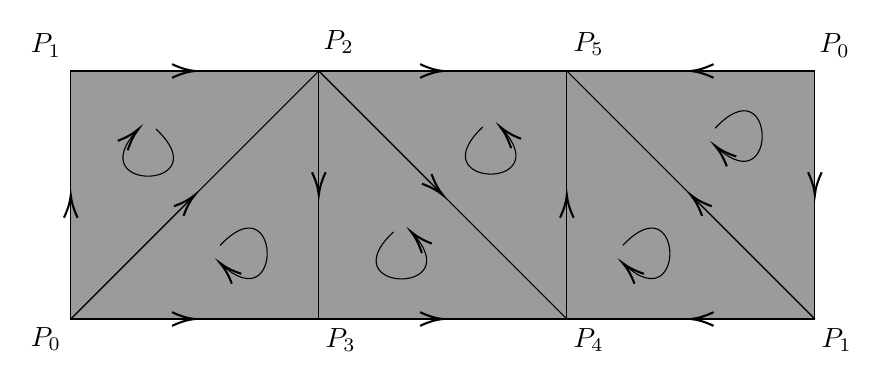
\begin{tikzpicture}[x=0.75pt,y=0.75pt,yscale=-1,xscale=1]
        %uncomment if require: \path (0,735); %set diagram left start at 0, and has height of 735

        %Shape: Polygon [id:ds012901580416037284] 
        \draw  [fill={rgb, 255:red, 155; green, 155; blue, 155 }  ,fill opacity=1 ] (440,55.5) -- (440,175) -- (81.5,175) -- (81.5,55.5) -- cycle ;
        %Straight Lines [id:da7117464125713011] 
        \draw    (81.5,55.5) -- (201,55.5) ;
        %Straight Lines [id:da8593345105117205] 
        \draw    (201,55.5) -- (320.5,55.5) ;
        %Straight Lines [id:da3706532081604941] 
        \draw    (320.5,55.5) -- (440,55.5) ;
        %Straight Lines [id:da5527262236568335] 
        \draw    (81.5,175) -- (201,175) ;
        %Straight Lines [id:da6652833889288519] 
        \draw    (201,175) -- (320.5,175) ;
        %Straight Lines [id:da2635536835037924] 
        \draw    (320.5,175) -- (440,175) ;
        %Straight Lines [id:da7627774994062366] 
        \draw    (81.5,55.5) -- (81.5,175) ;
        %Straight Lines [id:da5611032436091536] 
        \draw    (201,55.5) -- (201,175) ;
        %Straight Lines [id:da5168532258652223] 
        \draw    (320.5,55.5) -- (320.5,175) ;
        %Straight Lines [id:da6975191425087921] 
        \draw    (440,55.5) -- (440,175) ;
        %Straight Lines [id:da7664706882169221] 
        \draw    (201,55.5) -- (81.5,175) ;
        %Straight Lines [id:da7670217078686072] 
        \draw    (320.5,175) -- (201,55.5) ;
        %Straight Lines [id:da32965091603665986] 
        \draw    (440,175) -- (320.5,55.5) ;
        %Straight Lines [id:da14826879708125862] 
        \draw    (81.5,55.5) -- (139.25,55.5) ;
        \draw [shift={(141.25,55.5)}, rotate = 180] [color={rgb, 255:red, 0; green, 0; blue, 0 }  ][line width=0.75]    (10.93,-3.29) .. controls (6.95,-1.4) and (3.31,-0.3) .. (0,0) .. controls (3.31,0.3) and (6.95,1.4) .. (10.93,3.29)   ;
        %Straight Lines [id:da15072070377450997] 
        \draw    (201,55.5) -- (258.75,55.5) ;
        \draw [shift={(260.75,55.5)}, rotate = 180] [color={rgb, 255:red, 0; green, 0; blue, 0 }  ][line width=0.75]    (10.93,-3.29) .. controls (6.95,-1.4) and (3.31,-0.3) .. (0,0) .. controls (3.31,0.3) and (6.95,1.4) .. (10.93,3.29)   ;
        %Straight Lines [id:da2637515595976361] 
        \draw    (81.5,175) -- (139.25,175) ;
        \draw [shift={(141.25,175)}, rotate = 180] [color={rgb, 255:red, 0; green, 0; blue, 0 }  ][line width=0.75]    (10.93,-3.29) .. controls (6.95,-1.4) and (3.31,-0.3) .. (0,0) .. controls (3.31,0.3) and (6.95,1.4) .. (10.93,3.29)   ;
        %Straight Lines [id:da480909502322179] 
        \draw    (201,175) -- (258.75,175) ;
        \draw [shift={(260.75,175)}, rotate = 180] [color={rgb, 255:red, 0; green, 0; blue, 0 }  ][line width=0.75]    (10.93,-3.29) .. controls (6.95,-1.4) and (3.31,-0.3) .. (0,0) .. controls (3.31,0.3) and (6.95,1.4) .. (10.93,3.29)   ;
        %Straight Lines [id:da045805197883367565] 
        \draw    (81.5,175) -- (81.5,117.25) ;
        \draw [shift={(81.5,115.25)}, rotate = 90] [color={rgb, 255:red, 0; green, 0; blue, 0 }  ][line width=0.75]    (10.93,-3.29) .. controls (6.95,-1.4) and (3.31,-0.3) .. (0,0) .. controls (3.31,0.3) and (6.95,1.4) .. (10.93,3.29)   ;
        %Straight Lines [id:da3614729018304863] 
        \draw    (320.5,175) -- (320.5,117.25) ;
        \draw [shift={(320.5,115.25)}, rotate = 90] [color={rgb, 255:red, 0; green, 0; blue, 0 }  ][line width=0.75]    (10.93,-3.29) .. controls (6.95,-1.4) and (3.31,-0.3) .. (0,0) .. controls (3.31,0.3) and (6.95,1.4) .. (10.93,3.29)   ;
        %Straight Lines [id:da886918456601069] 
        \draw    (201,55.5) -- (201,113.25) ;
        \draw [shift={(201,115.25)}, rotate = 270] [color={rgb, 255:red, 0; green, 0; blue, 0 }  ][line width=0.75]    (10.93,-3.29) .. controls (6.95,-1.4) and (3.31,-0.3) .. (0,0) .. controls (3.31,0.3) and (6.95,1.4) .. (10.93,3.29)   ;
        %Straight Lines [id:da7214198150676829] 
        \draw    (440,55.5) -- (440,113.25) ;
        \draw [shift={(440,115.25)}, rotate = 270] [color={rgb, 255:red, 0; green, 0; blue, 0 }  ][line width=0.75]    (10.93,-3.29) .. controls (6.95,-1.4) and (3.31,-0.3) .. (0,0) .. controls (3.31,0.3) and (6.95,1.4) .. (10.93,3.29)   ;
        %Straight Lines [id:da08924791803738064] 
        \draw    (440,55.5) -- (382.25,55.5) ;
        \draw [shift={(380.25,55.5)}, rotate = 360] [color={rgb, 255:red, 0; green, 0; blue, 0 }  ][line width=0.75]    (10.93,-3.29) .. controls (6.95,-1.4) and (3.31,-0.3) .. (0,0) .. controls (3.31,0.3) and (6.95,1.4) .. (10.93,3.29)   ;
        %Straight Lines [id:da7243907591249072] 
        \draw    (440,175) -- (382.25,175) ;
        \draw [shift={(380.25,175)}, rotate = 360] [color={rgb, 255:red, 0; green, 0; blue, 0 }  ][line width=0.75]    (10.93,-3.29) .. controls (6.95,-1.4) and (3.31,-0.3) .. (0,0) .. controls (3.31,0.3) and (6.95,1.4) .. (10.93,3.29)   ;
        %Straight Lines [id:da08854589580856342] 
        \draw    (440,175) -- (381.66,116.66) ;
        \draw [shift={(380.25,115.25)}, rotate = 45] [color={rgb, 255:red, 0; green, 0; blue, 0 }  ][line width=0.75]    (10.93,-3.29) .. controls (6.95,-1.4) and (3.31,-0.3) .. (0,0) .. controls (3.31,0.3) and (6.95,1.4) .. (10.93,3.29)   ;
        %Straight Lines [id:da08689365102480684] 
        \draw    (201,55.5) -- (259.34,113.84) ;
        \draw [shift={(260.75,115.25)}, rotate = 225] [color={rgb, 255:red, 0; green, 0; blue, 0 }  ][line width=0.75]    (10.93,-3.29) .. controls (6.95,-1.4) and (3.31,-0.3) .. (0,0) .. controls (3.31,0.3) and (6.95,1.4) .. (10.93,3.29)   ;
        %Straight Lines [id:da2589861639102189] 
        \draw    (81.5,175) -- (139.84,116.66) ;
        \draw [shift={(141.25,115.25)}, rotate = 135] [color={rgb, 255:red, 0; green, 0; blue, 0 }  ][line width=0.75]    (10.93,-3.29) .. controls (6.95,-1.4) and (3.31,-0.3) .. (0,0) .. controls (3.31,0.3) and (6.95,1.4) .. (10.93,3.29)   ;
        %Shape: Boxed Bezier Curve [id:dp8422472837475492] 
        \draw    (122.59,83.5) .. controls (153.61,112.56) and (86.65,114.45) .. (112.82,84.87) ;
        \draw [shift={(114.09,83.5)}, rotate = 133.58] [color={rgb, 255:red, 0; green, 0; blue, 0 }  ][line width=0.75]    (10.93,-3.29) .. controls (6.95,-1.4) and (3.31,-0.3) .. (0,0) .. controls (3.31,0.3) and (6.95,1.4) .. (10.93,3.29)   ;
        %Curve Lines [id:da40098449242503587] 
        \draw    (280,82.5) .. controls (248.97,111.56) and (315.94,113.45) .. (289.76,83.87) ;
        \draw [shift={(288.5,82.5)}, rotate = 46.42] [color={rgb, 255:red, 0; green, 0; blue, 0 }  ][line width=0.75]    (10.93,-3.29) .. controls (6.95,-1.4) and (3.31,-0.3) .. (0,0) .. controls (3.31,0.3) and (6.95,1.4) .. (10.93,3.29)   ;
        %Curve Lines [id:da15715628474253296] 
        \draw    (237,133) .. controls (205.97,162.06) and (272.94,163.95) .. (246.76,134.37) ;
        \draw [shift={(245.5,133)}, rotate = 46.42] [color={rgb, 255:red, 0; green, 0; blue, 0 }  ][line width=0.75]    (10.93,-3.29) .. controls (6.95,-1.4) and (3.31,-0.3) .. (0,0) .. controls (3.31,0.3) and (6.95,1.4) .. (10.93,3.29)   ;
        %Shape: Boxed Bezier Curve [id:dp813150427829481] 
        \draw    (153.45,139.55) .. controls (182.5,108.53) and (184.4,175.49) .. (154.82,149.31) ;
        \draw [shift={(153.45,148.05)}, rotate = 43.58] [color={rgb, 255:red, 0; green, 0; blue, 0 }  ][line width=0.75]    (10.93,-3.29) .. controls (6.95,-1.4) and (3.31,-0.3) .. (0,0) .. controls (3.31,0.3) and (6.95,1.4) .. (10.93,3.29)   ;
        %Shape: Boxed Bezier Curve [id:dp931511034223832] 
        \draw    (347.45,139.55) .. controls (376.5,108.53) and (378.4,175.49) .. (348.82,149.31) ;
        \draw [shift={(347.45,148.05)}, rotate = 43.58] [color={rgb, 255:red, 0; green, 0; blue, 0 }  ][line width=0.75]    (10.93,-3.29) .. controls (6.95,-1.4) and (3.31,-0.3) .. (0,0) .. controls (3.31,0.3) and (6.95,1.4) .. (10.93,3.29)   ;
        %Shape: Boxed Bezier Curve [id:dp07096352170433295] 
        \draw    (391.95,83.05) .. controls (421,52.03) and (422.9,118.99) .. (393.32,92.81) ;
        \draw [shift={(391.95,91.55)}, rotate = 43.58] [color={rgb, 255:red, 0; green, 0; blue, 0 }  ][line width=0.75]    (10.93,-3.29) .. controls (6.95,-1.4) and (3.31,-0.3) .. (0,0) .. controls (3.31,0.3) and (6.95,1.4) .. (10.93,3.29)   ;

        % Text Node
        \draw (61,177.9) node [anchor=north west][inner sep=0.75pt]    {$P_{0}$};
        % Text Node
        \draw (441,36.4) node [anchor=north west][inner sep=0.75pt]    {$P_{0}$};
        % Text Node
        \draw (61,36.4) node [anchor=north west][inner sep=0.75pt]    {$P_{1}$};
        % Text Node
        \draw (442,178.4) node [anchor=north west][inner sep=0.75pt]    {$P_{1}$};
        % Text Node
        \draw (203,178.4) node [anchor=north west][inner sep=0.75pt]    {$P_{3}$};
        % Text Node
        \draw (202,34.9) node [anchor=north west][inner sep=0.75pt]    {$P_{2}$};
        % Text Node
        \draw (322.5,178.4) node [anchor=north west][inner sep=0.75pt]    {$P_{4}$};
        % Text Node
        \draw (322.5,35.9) node [anchor=north west][inner sep=0.75pt]    {$P_{5}$};


    \end{tikzpicture}

\end{center}
\pagebreak
\paragraph{Catene}
\[
    C_2(M)=\left<[P_0,P_1,P_2],[P_0,P_1,P_5],[P_0,P_2,P_3],\right.
\]
\[x
    \left.[P_1,P_4,P_5],[P_2,P_3,P_4],[P_2,P_4,P_5]\right>\simeq\Z^6
\]
\\
\[
    C_1(M)=\left<[P_0,P_1],[P_0,P_2],[P_0,P_3],[P_0,P_5],[P_1,P_2],[P_1,P_4],\right.
\]
\[
    \left.[P_1,P_5],[P_2,P_3],[P_2,P_4],[P_2,P_5],[P_3,P_4],[P_4,P_5]\right>\simeq\Z^{12}
\]\\
\[
    C_0(M)=\gen{P_0,P_1,P_2,P_3,P_4,P_5}\simeq\Z^6
\]
\paragraph{Operatori bordo}
\[
    \partial_2:C_2(M)\ra C_1(M)
\]\\
\[
    \partial_2=\begin{blockarray}{rrrrrrl}
        [P_0,P_1,P_2] & [P_0,P_1,P_5] & [P_0,P_2,P_3] & [P_1,P_4,P_5] & [P_2,P_3,P_4] & [P_2,P_4,P_5]\\
        \begin{block}{[cccccc]l}
            1       & 1     & \cdot & \cdot & \cdot & \cdot\topstrut & [P_0,P_1]\\
            -1      & \cdot & 1     & \cdot & \cdot & \cdot & [P_0,P_2]\\
            \cdot   & \cdot & -1    & \cdot & \cdot & \cdot & [P_0,P_3]\\
            \cdot   & -1    & \cdot & \cdot & \cdot & \cdot & [P_0,P_5]\\
            1       & \cdot & \cdot & \cdot & \cdot & \cdot & [P_1,P_2]\\
            \cdot   & \cdot & \cdot & 1     & \cdot & \cdot & [P_1,P_4]\\
            \cdot   & 1     & \cdot & -1    & \cdot & \cdot & [P_1,P_5]\\
            \cdot   & \cdot & 1     & \cdot & 1     & \cdot & [P_2,P_3]\\
            \cdot   & \cdot & \cdot & \cdot & -1    & 1 & [P_2,P_4]\\
            \cdot   & \cdot & \cdot & \cdot & \cdot & -1 & [P_2,P_5]\\
            \cdot   & \cdot & \cdot & \cdot & 1     & \cdot & [P_3,P_4]\\
            \cdot   & \cdot & \cdot & 1     & \cdot & 1\botstrut & [P_4,P_5]\\
        \end{block}
    \end{blockarray}
\]\\
\[
    \partial_1:C_1(M)\ra C_0(M)
\]\\
\[
    \partial_1=\scalemath{0.75}{
        \begin{blockarray}{rrrrrrrrrrrrl}
            [P_0,P_0] & [P_0,P_0] & [P_0,P_0] & [P_0,P_0] & [P_0,P_0] & [P_0,P_0] & [P_0,P_0] & [P_0,P_0] & [P_0,P_0] & [P_0,P_0] & [P_0,P_0] & [P_0,P_0]\\
            \begin{block}{[cccccccccccc]l}
                -1      & -1    & -1    & -1    & \cdot & \cdot & \cdot & \cdot & \cdot & \cdot & \cdot & \cdot\topstrut & P_0\\
                1       & \cdot & \cdot & \cdot & -1    & -1    & -1    & \cdot & \cdot & \cdot & \cdot & \cdot & P_0\\
                \cdot   & 1     & \cdot & \cdot & 1     & \cdot & \cdot & -1    & -1    & -1    & \cdot & \cdot & P_0\\
                \cdot   & \cdot & 1     & \cdot & \cdot & \cdot & \cdot & 1     & \cdot & \cdot & -1    & \cdot & P_0\\
                \cdot   & \cdot & \cdot & \cdot & \cdot & 1     & \cdot & \cdot & 1     & \cdot & 1     & -1    & P_0\\
                \cdot   & \cdot & \cdot & 1     & \cdot & \cdot & 1     & \cdot & \cdot & 1     & \cdot & 1\botstrut & P_0\\
            \end{block}
        \end{blockarray}
    }
\]
\pagebreak
\paragraph{Calcolo i gruppi di omologia}
\[
    H_0(M)=\faktor{Z_0(M)}{B_0(M)}=\faktor{C_0(M)}{B_0(M)}=\faktor{C_0(M)}{Im\ \partial_1}\ (\simeq\Z\text{ per connessione di $|M|$})
\]
\[
    H_1(M)=\faktor{Z_1(M)}{B_1(M)}=\faktor{Ker\ \partial_1}{Im\ \partial_2}
\]
\[
    H_2(M)=\faktor{Z_2(M)}{B_2(M)}=\faktor{Z_2(M)}{\{0\}}=Ker\ \partial_2
\]
$\mathbf{\partial_2})$ Riducendo la matrice di $\partial_2$ in forma di Smith ottengo:
\[
    \partial_2=\scalemath{0.75}{\begin{blockarray}{rrrrrrl}
            [P_0,P_1,P_2] & [P_0,P_1,P_5] & [P_0,P_2,P_3] & [P_1,P_4,P_5] & [P_2,P_3,P_4] & [P_2,P_4,P_5] &\\
            \begin{block}{[cccccc]l}
                1       &\cdot  &\cdot  & \cdot  & \cdot  & \cdot\topstrut & [P_0,P_1]+[P_0,P_5]\\
                \cdot   &1      &\cdot  & \cdot  & \cdot  & \cdot & -[P_0,P_5]\\
                \cdot   &\cdot  &1      & \cdot  & \cdot  & \cdot & -[P_0,P_3]\\
                \cdot   &\cdot  &\cdot  & \cdot  & \cdot  & \cdot & [P_0,P_2]+[P_0,P_1]+[P_0,P_5]+[P_0,P_3]\\
                \cdot   &\cdot  &\cdot  & \cdot  & \cdot  & \cdot & [P_1,P_2]-[P_0,P_1]-[P_0,P_5]\\
                \cdot   &\cdot  &\cdot  & 1      & \cdot  & \cdot & [P_1,P_4]\\
                \cdot   &\cdot  &\cdot  & \cdot  & \cdot  & \cdot & [P_1,P_5]+[P_0,P_5]+[P_1,P_4]\\
                \cdot   &\cdot  &\cdot  & \cdot  & 1      & \cdot & [P_2,P_3]+[P_0,P_3]\\
                \cdot   &\cdot  &\cdot  & \cdot  & \cdot  & 1     & [P_2,P_4]+[P_2,P_3]+[P_0,P_3]\\
                \cdot   &\cdot  &\cdot  & \cdot  & \cdot  & \cdot & [P_2,P_5]+[P_2,P_4]+[P_2,P_3]+[P_0,P_3]\\
                \cdot   &\cdot  &\cdot  & \cdot  & \cdot  & \cdot & [P_3,P_4]-[P_2,P_3]-[P_0,P_3]\\
                \cdot   &\cdot  &\cdot  & \cdot  & \cdot  & \cdot\botstrut & [P_4,P_5]-[P_1,P_4]-[P_2,P_4]-[P_2,P_3]-[P_0,P_3]\\
            \end{block}
        \end{blockarray}
    }
\]
Ottengo quindi
\[
    H_2(M)=Ker\ \partial_2=\{0\}
\]
\[
    Im\ \partial_2=\left<[P_0,P_1]+[P_0,P_5],-[P_0,P_5],-[P_0,P_3],[P_1,P_4],\right.
\]
\[
    \left.[P_2,P_3]+[P_0,P_3],[P_2,P_4]+[P_2,P_3]+[P_0,P_3]\right>
\]
\paragraph{Attenzione} $Im\ \partial_2=B_1(M)$, ma la forma normale di Smith nasconde la natura geometrica del bordo
\begin{center}


    \tikzset{every picture/.style={line width=0.75pt}} %set default line width to 0.75pt        

    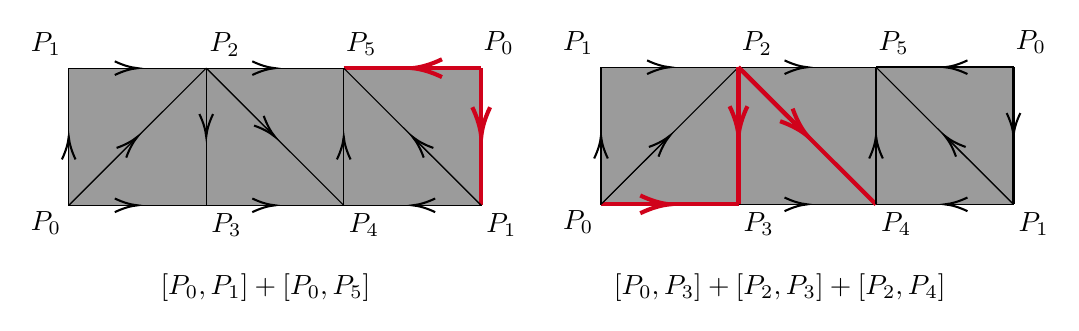
\begin{tikzpicture}[x=0.75pt,y=0.75pt,yscale=-1,xscale=1]
        %uncomment if require: \path (0,735); %set diagram left start at 0, and has height of 735

        %Shape: Polygon [id:ds012901580416037284] 
        \draw  [fill={rgb, 255:red, 155; green, 155; blue, 155 }  ,fill opacity=1 ] (272.57,39.59) -- (272.57,105.67) -- (73.83,105.67) -- (73.83,39.59) -- cycle ;
        %Straight Lines [id:da7117464125713011] 
        \draw    (73.83,39.59) -- (140.08,39.59) ;
        %Straight Lines [id:da8593345105117205] 
        \draw    (140.08,39.59) -- (206.33,39.59) ;
        %Straight Lines [id:da3706532081604941] 
        \draw [color={rgb, 255:red, 208; green, 2; blue, 27 }  ,draw opacity=1 ][line width=1.5]    (206.33,39.59) -- (272.57,39.59) ;
        %Straight Lines [id:da5527262236568335] 
        \draw    (73.83,105.67) -- (140.08,105.67) ;
        %Straight Lines [id:da6652833889288519] 
        \draw    (140.08,105.67) -- (206.33,105.67) ;
        %Straight Lines [id:da2635536835037924] 
        \draw    (206.33,105.67) -- (272.57,105.67) ;
        %Straight Lines [id:da7627774994062366] 
        \draw    (73.83,39.59) -- (73.83,105.67) ;
        %Straight Lines [id:da5611032436091536] 
        \draw    (140.08,39.59) -- (140.08,105.67) ;
        %Straight Lines [id:da5168532258652223] 
        \draw    (206.33,39.59) -- (206.33,105.67) ;
        %Straight Lines [id:da6975191425087921] 
        \draw [color={rgb, 255:red, 208; green, 2; blue, 27 }  ,draw opacity=1 ][line width=1.5]    (272.57,39.59) -- (272.57,105.67) ;
        %Straight Lines [id:da7664706882169221] 
        \draw    (140.08,39.59) -- (73.83,105.67) ;
        %Straight Lines [id:da7670217078686072] 
        \draw    (206.33,105.67) -- (140.08,39.59) ;
        %Straight Lines [id:da32965091603665986] 
        \draw    (272.57,105.67) -- (206.33,39.59) ;
        %Straight Lines [id:da14826879708125862] 
        \draw    (73.83,39.59) -- (104.96,39.59) ;
        \draw [shift={(106.96,39.59)}, rotate = 180] [color={rgb, 255:red, 0; green, 0; blue, 0 }  ][line width=0.75]    (10.93,-3.29) .. controls (6.95,-1.4) and (3.31,-0.3) .. (0,0) .. controls (3.31,0.3) and (6.95,1.4) .. (10.93,3.29)   ;
        %Straight Lines [id:da15072070377450997] 
        \draw    (140.08,39.59) -- (171.2,39.59) ;
        \draw [shift={(173.2,39.59)}, rotate = 180] [color={rgb, 255:red, 0; green, 0; blue, 0 }  ][line width=0.75]    (10.93,-3.29) .. controls (6.95,-1.4) and (3.31,-0.3) .. (0,0) .. controls (3.31,0.3) and (6.95,1.4) .. (10.93,3.29)   ;
        %Straight Lines [id:da2637515595976361] 
        \draw    (73.83,105.67) -- (104.96,105.67) ;
        \draw [shift={(106.96,105.67)}, rotate = 180] [color={rgb, 255:red, 0; green, 0; blue, 0 }  ][line width=0.75]    (10.93,-3.29) .. controls (6.95,-1.4) and (3.31,-0.3) .. (0,0) .. controls (3.31,0.3) and (6.95,1.4) .. (10.93,3.29)   ;
        %Straight Lines [id:da480909502322179] 
        \draw    (140.08,105.67) -- (171.2,105.67) ;
        \draw [shift={(173.2,105.67)}, rotate = 180] [color={rgb, 255:red, 0; green, 0; blue, 0 }  ][line width=0.75]    (10.93,-3.29) .. controls (6.95,-1.4) and (3.31,-0.3) .. (0,0) .. controls (3.31,0.3) and (6.95,1.4) .. (10.93,3.29)   ;
        %Straight Lines [id:da045805197883367565] 
        \draw    (73.83,105.67) -- (73.83,74.63) ;
        \draw [shift={(73.83,72.63)}, rotate = 90] [color={rgb, 255:red, 0; green, 0; blue, 0 }  ][line width=0.75]    (10.93,-3.29) .. controls (6.95,-1.4) and (3.31,-0.3) .. (0,0) .. controls (3.31,0.3) and (6.95,1.4) .. (10.93,3.29)   ;
        %Straight Lines [id:da3614729018304863] 
        \draw    (206.33,105.67) -- (206.33,74.63) ;
        \draw [shift={(206.33,72.63)}, rotate = 90] [color={rgb, 255:red, 0; green, 0; blue, 0 }  ][line width=0.75]    (10.93,-3.29) .. controls (6.95,-1.4) and (3.31,-0.3) .. (0,0) .. controls (3.31,0.3) and (6.95,1.4) .. (10.93,3.29)   ;
        %Straight Lines [id:da886918456601069] 
        \draw    (140.08,39.59) -- (140.08,70.63) ;
        \draw [shift={(140.08,72.63)}, rotate = 270] [color={rgb, 255:red, 0; green, 0; blue, 0 }  ][line width=0.75]    (10.93,-3.29) .. controls (6.95,-1.4) and (3.31,-0.3) .. (0,0) .. controls (3.31,0.3) and (6.95,1.4) .. (10.93,3.29)   ;
        %Straight Lines [id:da7214198150676829] 
        \draw [color={rgb, 255:red, 208; green, 2; blue, 27 }  ,draw opacity=1 ][line width=1.5]    (272.57,39.59) -- (272.57,69.63) ;
        \draw [shift={(272.57,72.63)}, rotate = 270] [color={rgb, 255:red, 208; green, 2; blue, 27 }  ,draw opacity=1 ][line width=1.5]    (14.21,-4.28) .. controls (9.04,-1.82) and (4.3,-0.39) .. (0,0) .. controls (4.3,0.39) and (9.04,1.82) .. (14.21,4.28)   ;
        %Straight Lines [id:da08924791803738064] 
        \draw [color={rgb, 255:red, 208; green, 2; blue, 27 }  ,draw opacity=1 ][line width=1.5]    (272.57,39.59) -- (242.45,39.59) ;
        \draw [shift={(239.45,39.59)}, rotate = 360] [color={rgb, 255:red, 208; green, 2; blue, 27 }  ,draw opacity=1 ][line width=1.5]    (14.21,-4.28) .. controls (9.04,-1.82) and (4.3,-0.39) .. (0,0) .. controls (4.3,0.39) and (9.04,1.82) .. (14.21,4.28)   ;
        %Straight Lines [id:da7243907591249072] 
        \draw    (272.57,105.67) -- (241.45,105.67) ;
        \draw [shift={(239.45,105.67)}, rotate = 360] [color={rgb, 255:red, 0; green, 0; blue, 0 }  ][line width=0.75]    (10.93,-3.29) .. controls (6.95,-1.4) and (3.31,-0.3) .. (0,0) .. controls (3.31,0.3) and (6.95,1.4) .. (10.93,3.29)   ;
        %Straight Lines [id:da08854589580856342] 
        \draw    (272.57,105.67) -- (240.86,74.04) ;
        \draw [shift={(239.45,72.63)}, rotate = 44.93] [color={rgb, 255:red, 0; green, 0; blue, 0 }  ][line width=0.75]    (10.93,-3.29) .. controls (6.95,-1.4) and (3.31,-0.3) .. (0,0) .. controls (3.31,0.3) and (6.95,1.4) .. (10.93,3.29)   ;
        %Straight Lines [id:da08689365102480684] 
        \draw    (140.08,39.59) -- (171.79,71.22) ;
        \draw [shift={(173.2,72.63)}, rotate = 224.93] [color={rgb, 255:red, 0; green, 0; blue, 0 }  ][line width=0.75]    (10.93,-3.29) .. controls (6.95,-1.4) and (3.31,-0.3) .. (0,0) .. controls (3.31,0.3) and (6.95,1.4) .. (10.93,3.29)   ;
        %Straight Lines [id:da2589861639102189] 
        \draw    (73.83,105.67) -- (105.54,74.04) ;
        \draw [shift={(106.96,72.63)}, rotate = 135.07] [color={rgb, 255:red, 0; green, 0; blue, 0 }  ][line width=0.75]    (10.93,-3.29) .. controls (6.95,-1.4) and (3.31,-0.3) .. (0,0) .. controls (3.31,0.3) and (6.95,1.4) .. (10.93,3.29)   ;
        %Shape: Polygon [id:ds4756108121461471] 
        \draw  [fill={rgb, 255:red, 155; green, 155; blue, 155 }  ,fill opacity=1 ] (529.02,39.13) -- (529.02,105.2) -- (330.28,105.2) -- (330.28,39.13) -- cycle ;
        %Straight Lines [id:da022548966734984743] 
        \draw    (330.28,39.13) -- (396.53,39.13) ;
        %Straight Lines [id:da3744297194625399] 
        \draw    (396.53,39.13) -- (462.78,39.13) ;
        %Straight Lines [id:da11282256571343785] 
        \draw [color={rgb, 255:red, 0; green, 0; blue, 0 }  ,draw opacity=1 ][line width=0.75]    (462.78,39.13) -- (529.02,39.13) ;
        %Straight Lines [id:da597932440304084] 
        \draw [color={rgb, 255:red, 208; green, 2; blue, 27 }  ,draw opacity=1 ][line width=1.5]    (330.28,105.2) -- (396.53,105.2) ;
        %Straight Lines [id:da7515335407063859] 
        \draw    (396.53,105.2) -- (462.78,105.2) ;
        %Straight Lines [id:da7849928818250089] 
        \draw    (462.78,105.2) -- (529.02,105.2) ;
        %Straight Lines [id:da9401555025247612] 
        \draw    (330.28,39.13) -- (330.28,105.2) ;
        %Straight Lines [id:da13883723123858926] 
        \draw [color={rgb, 255:red, 208; green, 2; blue, 27 }  ,draw opacity=1 ][line width=1.5]    (396.53,39.13) -- (396.53,105.2) ;
        %Straight Lines [id:da3487164426510623] 
        \draw    (462.78,39.13) -- (462.78,105.2) ;
        %Straight Lines [id:da3895939707071987] 
        \draw [color={rgb, 255:red, 0; green, 0; blue, 0 }  ,draw opacity=1 ][line width=0.75]    (529.02,39.13) -- (529.02,105.2) ;
        %Straight Lines [id:da14757014775773647] 
        \draw    (396.53,39.13) -- (330.28,105.2) ;
        %Straight Lines [id:da3622293596862749] 
        \draw [color={rgb, 255:red, 208; green, 2; blue, 27 }  ,draw opacity=1 ][line width=1.5]    (462.78,105.2) -- (396.53,39.13) ;
        %Straight Lines [id:da7880608666498556] 
        \draw    (529.02,105.2) -- (462.78,39.13) ;
        %Straight Lines [id:da16907653133529688] 
        \draw    (330.28,39.13) -- (361.41,39.13) ;
        \draw [shift={(363.41,39.13)}, rotate = 180] [color={rgb, 255:red, 0; green, 0; blue, 0 }  ][line width=0.75]    (10.93,-3.29) .. controls (6.95,-1.4) and (3.31,-0.3) .. (0,0) .. controls (3.31,0.3) and (6.95,1.4) .. (10.93,3.29)   ;
        %Straight Lines [id:da9859120988149876] 
        \draw    (396.53,39.13) -- (427.65,39.13) ;
        \draw [shift={(429.65,39.13)}, rotate = 180] [color={rgb, 255:red, 0; green, 0; blue, 0 }  ][line width=0.75]    (10.93,-3.29) .. controls (6.95,-1.4) and (3.31,-0.3) .. (0,0) .. controls (3.31,0.3) and (6.95,1.4) .. (10.93,3.29)   ;
        %Straight Lines [id:da5798371151840513] 
        \draw [color={rgb, 255:red, 208; green, 2; blue, 27 }  ,draw opacity=1 ][line width=1.5]    (330.28,105.2) -- (360.41,105.2) ;
        \draw [shift={(363.41,105.2)}, rotate = 180] [color={rgb, 255:red, 208; green, 2; blue, 27 }  ,draw opacity=1 ][line width=1.5]    (14.21,-4.28) .. controls (9.04,-1.82) and (4.3,-0.39) .. (0,0) .. controls (4.3,0.39) and (9.04,1.82) .. (14.21,4.28)   ;
        %Straight Lines [id:da4297052650173796] 
        \draw    (396.53,105.2) -- (427.65,105.2) ;
        \draw [shift={(429.65,105.2)}, rotate = 180] [color={rgb, 255:red, 0; green, 0; blue, 0 }  ][line width=0.75]    (10.93,-3.29) .. controls (6.95,-1.4) and (3.31,-0.3) .. (0,0) .. controls (3.31,0.3) and (6.95,1.4) .. (10.93,3.29)   ;
        %Straight Lines [id:da7550659455544337] 
        \draw    (330.28,105.2) -- (330.28,74.16) ;
        \draw [shift={(330.28,72.16)}, rotate = 90] [color={rgb, 255:red, 0; green, 0; blue, 0 }  ][line width=0.75]    (10.93,-3.29) .. controls (6.95,-1.4) and (3.31,-0.3) .. (0,0) .. controls (3.31,0.3) and (6.95,1.4) .. (10.93,3.29)   ;
        %Straight Lines [id:da4155571186794189] 
        \draw    (462.78,105.2) -- (462.78,74.16) ;
        \draw [shift={(462.78,72.16)}, rotate = 90] [color={rgb, 255:red, 0; green, 0; blue, 0 }  ][line width=0.75]    (10.93,-3.29) .. controls (6.95,-1.4) and (3.31,-0.3) .. (0,0) .. controls (3.31,0.3) and (6.95,1.4) .. (10.93,3.29)   ;
        %Straight Lines [id:da4773164769227365] 
        \draw [color={rgb, 255:red, 208; green, 2; blue, 27 }  ,draw opacity=1 ][line width=1.5]    (396.53,39.13) -- (396.53,69.16) ;
        \draw [shift={(396.53,72.16)}, rotate = 270] [color={rgb, 255:red, 208; green, 2; blue, 27 }  ,draw opacity=1 ][line width=1.5]    (14.21,-4.28) .. controls (9.04,-1.82) and (4.3,-0.39) .. (0,0) .. controls (4.3,0.39) and (9.04,1.82) .. (14.21,4.28)   ;
        %Straight Lines [id:da5459171065916391] 
        \draw [color={rgb, 255:red, 0; green, 0; blue, 0 }  ,draw opacity=1 ][line width=0.75]    (529.02,39.13) -- (529.02,70.16) ;
        \draw [shift={(529.02,72.16)}, rotate = 270] [color={rgb, 255:red, 0; green, 0; blue, 0 }  ,draw opacity=1 ][line width=0.75]    (10.93,-3.29) .. controls (6.95,-1.4) and (3.31,-0.3) .. (0,0) .. controls (3.31,0.3) and (6.95,1.4) .. (10.93,3.29)   ;
        %Straight Lines [id:da7783618228032774] 
        \draw [color={rgb, 255:red, 0; green, 0; blue, 0 }  ,draw opacity=1 ][line width=0.75]    (529.02,39.13) -- (497.9,39.13) ;
        \draw [shift={(495.9,39.13)}, rotate = 360] [color={rgb, 255:red, 0; green, 0; blue, 0 }  ,draw opacity=1 ][line width=0.75]    (10.93,-3.29) .. controls (6.95,-1.4) and (3.31,-0.3) .. (0,0) .. controls (3.31,0.3) and (6.95,1.4) .. (10.93,3.29)   ;
        %Straight Lines [id:da5715371215845164] 
        \draw    (529.02,105.2) -- (497.9,105.2) ;
        \draw [shift={(495.9,105.2)}, rotate = 360] [color={rgb, 255:red, 0; green, 0; blue, 0 }  ][line width=0.75]    (10.93,-3.29) .. controls (6.95,-1.4) and (3.31,-0.3) .. (0,0) .. controls (3.31,0.3) and (6.95,1.4) .. (10.93,3.29)   ;
        %Straight Lines [id:da05084149170057928] 
        \draw    (529.02,105.2) -- (497.31,73.58) ;
        \draw [shift={(495.9,72.16)}, rotate = 44.93] [color={rgb, 255:red, 0; green, 0; blue, 0 }  ][line width=0.75]    (10.93,-3.29) .. controls (6.95,-1.4) and (3.31,-0.3) .. (0,0) .. controls (3.31,0.3) and (6.95,1.4) .. (10.93,3.29)   ;
        %Straight Lines [id:da6790721651710836] 
        \draw [color={rgb, 255:red, 208; green, 2; blue, 27 }  ,draw opacity=1 ][line width=1.5]    (396.53,39.13) -- (427.53,70.05) ;
        \draw [shift={(429.65,72.16)}, rotate = 224.93] [color={rgb, 255:red, 208; green, 2; blue, 27 }  ,draw opacity=1 ][line width=1.5]    (14.21,-4.28) .. controls (9.04,-1.82) and (4.3,-0.39) .. (0,0) .. controls (4.3,0.39) and (9.04,1.82) .. (14.21,4.28)   ;
        %Straight Lines [id:da12584966462533176] 
        \draw    (330.28,105.2) -- (361.99,73.58) ;
        \draw [shift={(363.41,72.16)}, rotate = 135.07] [color={rgb, 255:red, 0; green, 0; blue, 0 }  ][line width=0.75]    (10.93,-3.29) .. controls (6.95,-1.4) and (3.31,-0.3) .. (0,0) .. controls (3.31,0.3) and (6.95,1.4) .. (10.93,3.29)   ;

        % Text Node
        \draw (54.32,107.41) node [anchor=north west][inner sep=0.75pt]    {$P_{0}$};
        % Text Node
        \draw (272.43,20.82) node [anchor=north west][inner sep=0.75pt]    {$P_{0}$};
        % Text Node
        \draw (54.32,21.28) node [anchor=north west][inner sep=0.75pt]    {$P_{1}$};
        % Text Node
        \draw (273.78,108.21) node [anchor=north west][inner sep=0.75pt]    {$P_{1}$};
        % Text Node
        \draw (141.28,108.21) node [anchor=north west][inner sep=0.75pt]    {$P_{3}$};
        % Text Node
        \draw (140.4,21.38) node [anchor=north west][inner sep=0.75pt]    {$P_{2}$};
        % Text Node
        \draw (207.53,108.21) node [anchor=north west][inner sep=0.75pt]    {$P_{4}$};
        % Text Node
        \draw (206.27,21.01) node [anchor=north west][inner sep=0.75pt]    {$P_{5}$};
        % Text Node
        \draw (310.78,106.95) node [anchor=north west][inner sep=0.75pt]    {$P_{0}$};
        % Text Node
        \draw (528.88,20.35) node [anchor=north west][inner sep=0.75pt]    {$P_{0}$};
        % Text Node
        \draw (310.78,20.82) node [anchor=north west][inner sep=0.75pt]    {$P_{1}$};
        % Text Node
        \draw (530.23,107.74) node [anchor=north west][inner sep=0.75pt]    {$P_{1}$};
        % Text Node
        \draw (397.74,107.74) node [anchor=north west][inner sep=0.75pt]    {$P_{3}$};
        % Text Node
        \draw (396.85,20.92) node [anchor=north west][inner sep=0.75pt]    {$P_{2}$};
        % Text Node
        \draw (463.98,107.74) node [anchor=north west][inner sep=0.75pt]    {$P_{4}$};
        % Text Node
        \draw (462.72,20.54) node [anchor=north west][inner sep=0.75pt]    {$P_{5}$};
        % Text Node
        \draw (116.79,137.19) node [anchor=north west][inner sep=0.75pt]    {$[ P_{0} ,P_{1}] +[ P_{0} ,P_{5}]$};
        % Text Node
        \draw (335.21,137.22) node [anchor=north west][inner sep=0.75pt]    {$[ P_{0} ,P_{3}] +[ P_{2} ,P_{3}] +[ P_{2} ,P_{4}]$};


    \end{tikzpicture}

\end{center}
Non è facile trovare il giusto equilibrio tra efficienza algebrica e interpretazione geometrica\newpage
$\mathbf{\partial_1})$ Riducendo la matrice di $\partial_1$ in forma di Smith (senza cancellare le colonne che non contengono pivot) ottengo:
\[
    \partial_1=\scalemath{0.75}{\begin{blockarray}{rrrrrrrrrrrr}
            [P_0,P_1] & [P_0,P_2] & [P_0,P_3] & [P_0,P_5] & [P_1,P_2] & [P_1,P_4] & [P_1,P_5] & [P_2,P_3] & [P_2,P_4] & [P_2,P_5] & [P_3,P_4] & [P_4,P_5] &\\
            \begin{block}{[cccccccccccc]}
                -1      & \cdot & \cdot & \cdot & 1     & \cdot & 1     & \cdot & -1    & \cdot & -1    & 1\topstrut\\
                \cdot   & -1    & \cdot & \cdot & -1    & \cdot & \cdot & 1     & 1     & 1     & \cdot & \cdot\\
                \cdot   & \cdot & -1    & \cdot & \cdot & \cdot & \cdot & -1    & \cdot & \cdot & 1     & \cdot\\
                \cdot   & \cdot & \cdot & -1    & \cdot & \cdot & -1    & \cdot & \cdot & -1    & \cdot & -1\\
                \cdot   & \cdot & \cdot & \cdot & \cdot & 1     & \cdot & \cdot & 1     & \cdot & 1     & -1\botstrut\\
            \end{block}
        \end{blockarray}
    }
\]
Ottengo quindi
\[
    Ker\ \partial_1=\left<[P_1,P_2]+[P_0,P_1]-[P_0,P_2],[P_1,P_5]+[P_0,P_1]-[P_0,P_5],\right.
\]
\[
    [P_2,P_3]+[P_0,P_2]-[P_0,P_3],[P_2,P_4]-[P_0,P_1]+[P_0,P_2]-[P_1,P_4],
\]
\[
    [P_2,P_5]+[P_0,P_2]-[P_0,P_5],[P_3,P_4]-[P_0,P_1]+[P_0,P_3]-[P_1,P_4],
\]
\[
    \left.[P_4,P_5]+[P_0,P_1]-[P_0,P_5]+[P_1,P_4]\right>\simeq\Z^7
\]
\begin{center}


    \tikzset{every picture/.style={line width=0.75pt}} %set default line width to 0.75pt        

    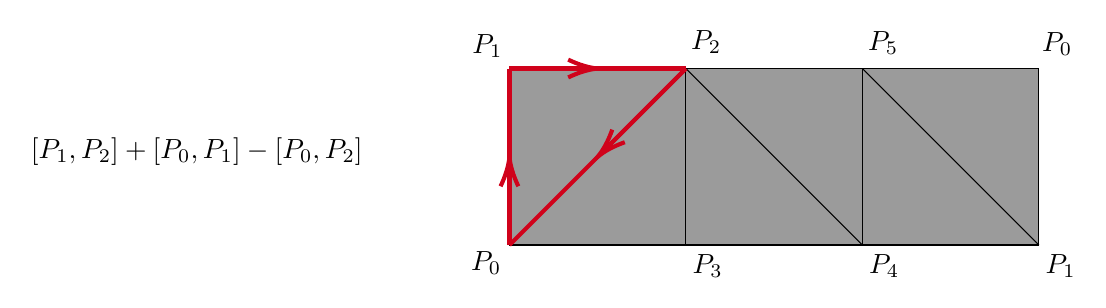
\begin{tikzpicture}[x=0.75pt,y=0.75pt,yscale=-1,xscale=1]
        %uncomment if require: \path (0,735); %set diagram left start at 0, and has height of 735

        %Shape: Polygon [id:ds012901580416037284] 
        \draw  [fill={rgb, 255:red, 155; green, 155; blue, 155 }  ,fill opacity=1 ] (510.43,41.9) -- (510.43,126.93) -- (255.35,126.93) -- (255.35,41.9) -- cycle ;
        %Straight Lines [id:da7117464125713011] 
        \draw [color={rgb, 255:red, 208; green, 2; blue, 27 }  ,draw opacity=1 ][line width=1.5]    (255.35,41.9) -- (340.37,41.9) ;
        %Straight Lines [id:da8593345105117205] 
        \draw    (340.37,41.9) -- (425.4,41.9) ;
        %Straight Lines [id:da3706532081604941] 
        \draw    (425.4,41.9) -- (510.43,41.9) ;
        %Straight Lines [id:da5527262236568335] 
        \draw    (255.35,126.93) -- (340.37,126.93) ;
        %Straight Lines [id:da6652833889288519] 
        \draw    (340.37,126.93) -- (425.4,126.93) ;
        %Straight Lines [id:da2635536835037924] 
        \draw    (425.4,126.93) -- (510.43,126.93) ;
        %Straight Lines [id:da7627774994062366] 
        \draw [color={rgb, 255:red, 208; green, 2; blue, 27 }  ,draw opacity=1 ][line width=1.5]    (255.35,41.9) -- (255.35,126.93) ;
        %Straight Lines [id:da5611032436091536] 
        \draw    (340.37,41.9) -- (340.37,126.93) ;
        %Straight Lines [id:da5168532258652223] 
        \draw    (425.4,41.9) -- (425.4,126.93) ;
        %Straight Lines [id:da6975191425087921] 
        \draw    (510.43,41.9) -- (510.43,126.93) ;
        %Straight Lines [id:da7664706882169221] 
        \draw [color={rgb, 255:red, 208; green, 2; blue, 27 }  ,draw opacity=1 ][line width=1.5]    (340.37,41.9) -- (255.35,126.93) ;
        %Straight Lines [id:da7670217078686072] 
        \draw    (425.4,126.93) -- (340.37,41.9) ;
        %Straight Lines [id:da32965091603665986] 
        \draw    (510.43,126.93) -- (425.4,41.9) ;
        %Straight Lines [id:da14826879708125862] 
        \draw [color={rgb, 255:red, 208; green, 2; blue, 27 }  ,draw opacity=1 ][line width=1.5]    (255.35,41.9) -- (294.86,41.9) ;
        \draw [shift={(297.86,41.9)}, rotate = 180] [color={rgb, 255:red, 208; green, 2; blue, 27 }  ,draw opacity=1 ][line width=1.5]    (14.21,-4.28) .. controls (9.04,-1.82) and (4.3,-0.39) .. (0,0) .. controls (4.3,0.39) and (9.04,1.82) .. (14.21,4.28)   ;
        %Straight Lines [id:da045805197883367565] 
        \draw [color={rgb, 255:red, 208; green, 2; blue, 27 }  ,draw opacity=1 ][line width=1.5]    (255.35,126.93) -- (255.35,87.42) ;
        \draw [shift={(255.35,84.42)}, rotate = 90] [color={rgb, 255:red, 208; green, 2; blue, 27 }  ,draw opacity=1 ][line width=1.5]    (14.21,-4.28) .. controls (9.04,-1.82) and (4.3,-0.39) .. (0,0) .. controls (4.3,0.39) and (9.04,1.82) .. (14.21,4.28)   ;
        %Straight Lines [id:da2589861639102189] 
        \draw [color={rgb, 255:red, 208; green, 2; blue, 27 }  ,draw opacity=1 ][line width=1.5]    (340.37,41.9) -- (299.98,82.29) ;
        \draw [shift={(297.86,84.42)}, rotate = 315] [color={rgb, 255:red, 208; green, 2; blue, 27 }  ,draw opacity=1 ][line width=1.5]    (14.21,-4.28) .. controls (9.04,-1.82) and (4.3,-0.39) .. (0,0) .. controls (4.3,0.39) and (9.04,1.82) .. (14.21,4.28)   ;

        % Text Node
        \draw (235.63,128.85) node [anchor=north west][inner sep=0.75pt]    {$P_{0}$};
        % Text Node
        \draw (510.73,23.11) node [anchor=north west][inner sep=0.75pt]    {$P_{0}$};
        % Text Node
        \draw (236.24,24.05) node [anchor=north west][inner sep=0.75pt]    {$P_{1}$};
        % Text Node
        \draw (512.43,130.33) node [anchor=north west][inner sep=0.75pt]    {$P_{1}$};
        % Text Node
        \draw (342.37,130.33) node [anchor=north west][inner sep=0.75pt]    {$P_{3}$};
        % Text Node
        \draw (341.62,22.48) node [anchor=north west][inner sep=0.75pt]    {$P_{2}$};
        % Text Node
        \draw (427.4,130.33) node [anchor=north west][inner sep=0.75pt]    {$P_{4}$};
        % Text Node
        \draw (426.86,22.7) node [anchor=north west][inner sep=0.75pt]    {$P_{5}$};
        % Text Node
        \draw (23.5,73.9) node [anchor=north west][inner sep=0.75pt]    {$[ P_{1} ,P_{2}] +[ P_{0} ,P_{1}] -[ P_{0} ,P_{2}]$};


    \end{tikzpicture}

\end{center}
\begin{center}


    \tikzset{every picture/.style={line width=0.75pt}} %set default line width to 0.75pt        

    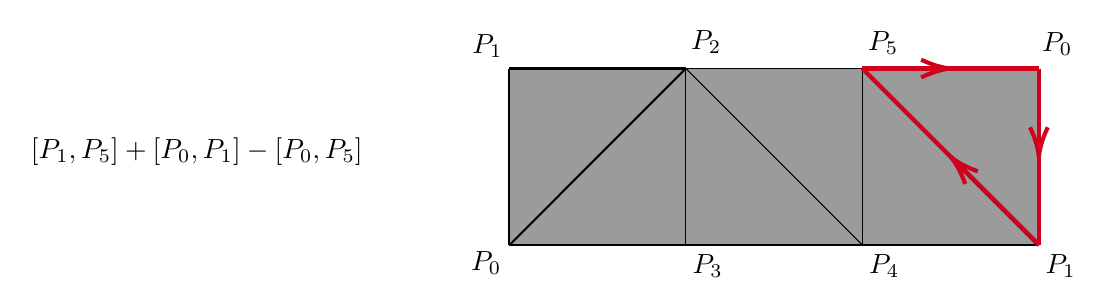
\begin{tikzpicture}[x=0.75pt,y=0.75pt,yscale=-1,xscale=1]
        %uncomment if require: \path (0,735); %set diagram left start at 0, and has height of 735

        %Shape: Polygon [id:ds012901580416037284] 
        \draw  [fill={rgb, 255:red, 155; green, 155; blue, 155 }  ,fill opacity=1 ] (510.43,41.9) -- (510.43,126.93) -- (255.35,126.93) -- (255.35,41.9) -- cycle ;
        %Straight Lines [id:da7117464125713011] 
        \draw [color={rgb, 255:red, 0; green, 0; blue, 0 }  ,draw opacity=1 ][line width=0.75]    (255.35,41.9) -- (340.37,41.9) ;
        %Straight Lines [id:da8593345105117205] 
        \draw    (340.37,41.9) -- (425.4,41.9) ;
        %Straight Lines [id:da3706532081604941] 
        \draw [color={rgb, 255:red, 208; green, 2; blue, 27 }  ,draw opacity=1 ][line width=1.5]    (425.4,41.9) -- (510.43,41.9) ;
        %Straight Lines [id:da5527262236568335] 
        \draw    (255.35,126.93) -- (340.37,126.93) ;
        %Straight Lines [id:da6652833889288519] 
        \draw    (340.37,126.93) -- (425.4,126.93) ;
        %Straight Lines [id:da2635536835037924] 
        \draw    (425.4,126.93) -- (510.43,126.93) ;
        %Straight Lines [id:da7627774994062366] 
        \draw [color={rgb, 255:red, 0; green, 0; blue, 0 }  ,draw opacity=1 ][line width=0.75]    (255.35,41.9) -- (255.35,126.93) ;
        %Straight Lines [id:da5611032436091536] 
        \draw    (340.37,41.9) -- (340.37,126.93) ;
        %Straight Lines [id:da5168532258652223] 
        \draw    (425.4,41.9) -- (425.4,126.93) ;
        %Straight Lines [id:da6975191425087921] 
        \draw [color={rgb, 255:red, 208; green, 2; blue, 27 }  ,draw opacity=1 ][line width=1.5]    (510.43,41.9) -- (510.43,126.93) ;
        %Straight Lines [id:da7664706882169221] 
        \draw [color={rgb, 255:red, 0; green, 0; blue, 0 }  ,draw opacity=1 ][line width=0.75]    (340.37,41.9) -- (255.35,126.93) ;
        %Straight Lines [id:da7670217078686072] 
        \draw    (425.4,126.93) -- (340.37,41.9) ;
        %Straight Lines [id:da32965091603665986] 
        \draw [color={rgb, 255:red, 208; green, 2; blue, 27 }  ,draw opacity=1 ][line width=1.5]    (510.43,126.93) -- (425.4,41.9) ;
        %Straight Lines [id:da14826879708125862] 
        \draw [color={rgb, 255:red, 208; green, 2; blue, 27 }  ,draw opacity=1 ][line width=1.5]    (510.43,41.9) -- (510.43,81.42) ;
        \draw [shift={(510.43,84.42)}, rotate = 270] [color={rgb, 255:red, 208; green, 2; blue, 27 }  ,draw opacity=1 ][line width=1.5]    (14.21,-4.28) .. controls (9.04,-1.82) and (4.3,-0.39) .. (0,0) .. controls (4.3,0.39) and (9.04,1.82) .. (14.21,4.28)   ;
        %Straight Lines [id:da045805197883367565] 
        \draw [color={rgb, 255:red, 208; green, 2; blue, 27 }  ,draw opacity=1 ][line width=1.5]    (510.43,126.93) -- (470.03,86.54) ;
        \draw [shift={(467.91,84.42)}, rotate = 45] [color={rgb, 255:red, 208; green, 2; blue, 27 }  ,draw opacity=1 ][line width=1.5]    (14.21,-4.28) .. controls (9.04,-1.82) and (4.3,-0.39) .. (0,0) .. controls (4.3,0.39) and (9.04,1.82) .. (14.21,4.28)   ;
        %Straight Lines [id:da2589861639102189] 
        \draw [color={rgb, 255:red, 208; green, 2; blue, 27 }  ,draw opacity=1 ][line width=1.5]    (425.4,41.9) -- (464.91,41.9) ;
        \draw [shift={(467.91,41.9)}, rotate = 180] [color={rgb, 255:red, 208; green, 2; blue, 27 }  ,draw opacity=1 ][line width=1.5]    (14.21,-4.28) .. controls (9.04,-1.82) and (4.3,-0.39) .. (0,0) .. controls (4.3,0.39) and (9.04,1.82) .. (14.21,4.28)   ;

        % Text Node
        \draw (235.63,128.85) node [anchor=north west][inner sep=0.75pt]    {$P_{0}$};
        % Text Node
        \draw (510.73,23.11) node [anchor=north west][inner sep=0.75pt]    {$P_{0}$};
        % Text Node
        \draw (236.24,24.05) node [anchor=north west][inner sep=0.75pt]    {$P_{1}$};
        % Text Node
        \draw (512.43,130.33) node [anchor=north west][inner sep=0.75pt]    {$P_{1}$};
        % Text Node
        \draw (342.37,130.33) node [anchor=north west][inner sep=0.75pt]    {$P_{3}$};
        % Text Node
        \draw (341.62,22.48) node [anchor=north west][inner sep=0.75pt]    {$P_{2}$};
        % Text Node
        \draw (427.4,130.33) node [anchor=north west][inner sep=0.75pt]    {$P_{4}$};
        % Text Node
        \draw (426.86,22.7) node [anchor=north west][inner sep=0.75pt]    {$P_{5}$};
        % Text Node
        \draw (23.5,73.9) node [anchor=north west][inner sep=0.75pt]    {$[ P_{1} ,P_{5}] +[ P_{0} ,P_{1}] -[ P_{0} ,P_{5}]$};


    \end{tikzpicture}
\end{center}
\begin{center}


    \tikzset{every picture/.style={line width=0.75pt}} %set default line width to 0.75pt        

    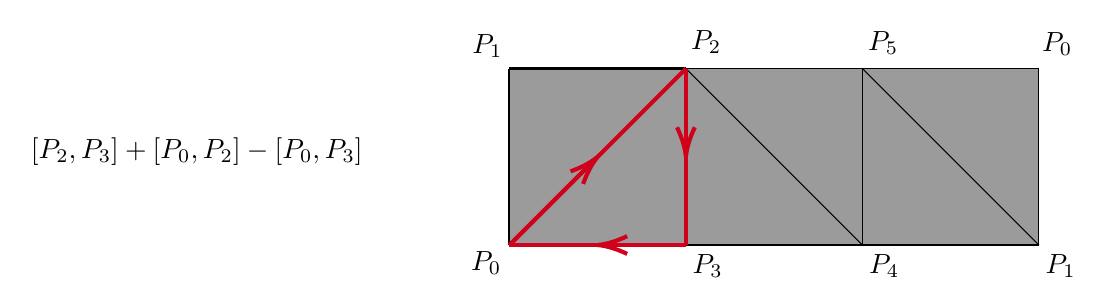
\begin{tikzpicture}[x=0.75pt,y=0.75pt,yscale=-1,xscale=1]
        %uncomment if require: \path (0,735); %set diagram left start at 0, and has height of 735

        %Shape: Polygon [id:ds012901580416037284] 
        \draw  [fill={rgb, 255:red, 155; green, 155; blue, 155 }  ,fill opacity=1 ] (510.43,41.9) -- (510.43,126.93) -- (255.35,126.93) -- (255.35,41.9) -- cycle ;
        %Straight Lines [id:da7117464125713011] 
        \draw [color={rgb, 255:red, 0; green, 0; blue, 0 }  ,draw opacity=1 ][line width=0.75]    (255.35,41.9) -- (340.37,41.9) ;
        %Straight Lines [id:da8593345105117205] 
        \draw    (340.37,41.9) -- (425.4,41.9) ;
        %Straight Lines [id:da3706532081604941] 
        \draw    (425.4,41.9) -- (510.43,41.9) ;
        %Straight Lines [id:da5527262236568335] 
        \draw [color={rgb, 255:red, 208; green, 2; blue, 27 }  ,draw opacity=1 ][line width=1.5]    (255.35,126.93) -- (340.37,126.93) ;
        %Straight Lines [id:da6652833889288519] 
        \draw    (340.37,126.93) -- (425.4,126.93) ;
        %Straight Lines [id:da2635536835037924] 
        \draw    (425.4,126.93) -- (510.43,126.93) ;
        %Straight Lines [id:da7627774994062366] 
        \draw [color={rgb, 255:red, 0; green, 0; blue, 0 }  ,draw opacity=1 ][line width=0.75]    (255.35,41.9) -- (255.35,126.93) ;
        %Straight Lines [id:da5611032436091536] 
        \draw [color={rgb, 255:red, 208; green, 2; blue, 27 }  ,draw opacity=1 ][line width=1.5]    (340.37,41.9) -- (340.37,126.93) ;
        %Straight Lines [id:da5168532258652223] 
        \draw    (425.4,41.9) -- (425.4,126.93) ;
        %Straight Lines [id:da6975191425087921] 
        \draw    (510.43,41.9) -- (510.43,126.93) ;
        %Straight Lines [id:da7664706882169221] 
        \draw [color={rgb, 255:red, 208; green, 2; blue, 27 }  ,draw opacity=1 ][line width=1.5]    (340.37,41.9) -- (255.35,126.93) ;
        %Straight Lines [id:da7670217078686072] 
        \draw    (425.4,126.93) -- (340.37,41.9) ;
        %Straight Lines [id:da32965091603665986] 
        \draw    (510.43,126.93) -- (425.4,41.9) ;
        %Straight Lines [id:da14826879708125862] 
        \draw [color={rgb, 255:red, 208; green, 2; blue, 27 }  ,draw opacity=1 ][line width=1.5]    (340.37,41.9) -- (340.37,76.5) -- (340.37,81.42) ;
        \draw [shift={(340.37,84.42)}, rotate = 270] [color={rgb, 255:red, 208; green, 2; blue, 27 }  ,draw opacity=1 ][line width=1.5]    (14.21,-4.28) .. controls (9.04,-1.82) and (4.3,-0.39) .. (0,0) .. controls (4.3,0.39) and (9.04,1.82) .. (14.21,4.28)   ;
        %Straight Lines [id:da045805197883367565] 
        \draw [color={rgb, 255:red, 208; green, 2; blue, 27 }  ,draw opacity=1 ][line width=1.5]    (255.35,126.93) -- (295.74,86.54) ;
        \draw [shift={(297.86,84.42)}, rotate = 135] [color={rgb, 255:red, 208; green, 2; blue, 27 }  ,draw opacity=1 ][line width=1.5]    (14.21,-4.28) .. controls (9.04,-1.82) and (4.3,-0.39) .. (0,0) .. controls (4.3,0.39) and (9.04,1.82) .. (14.21,4.28)   ;
        %Straight Lines [id:da2589861639102189] 
        \draw [color={rgb, 255:red, 208; green, 2; blue, 27 }  ,draw opacity=1 ][line width=1.5]    (340.37,126.93) -- (300.86,126.93) ;
        \draw [shift={(297.86,126.93)}, rotate = 360] [color={rgb, 255:red, 208; green, 2; blue, 27 }  ,draw opacity=1 ][line width=1.5]    (14.21,-4.28) .. controls (9.04,-1.82) and (4.3,-0.39) .. (0,0) .. controls (4.3,0.39) and (9.04,1.82) .. (14.21,4.28)   ;

        % Text Node
        \draw (235.63,128.85) node [anchor=north west][inner sep=0.75pt]    {$P_{0}$};
        % Text Node
        \draw (510.73,23.11) node [anchor=north west][inner sep=0.75pt]    {$P_{0}$};
        % Text Node
        \draw (236.24,24.05) node [anchor=north west][inner sep=0.75pt]    {$P_{1}$};
        % Text Node
        \draw (512.43,130.33) node [anchor=north west][inner sep=0.75pt]    {$P_{1}$};
        % Text Node
        \draw (342.37,130.33) node [anchor=north west][inner sep=0.75pt]    {$P_{3}$};
        % Text Node
        \draw (341.62,22.48) node [anchor=north west][inner sep=0.75pt]    {$P_{2}$};
        % Text Node
        \draw (427.4,130.33) node [anchor=north west][inner sep=0.75pt]    {$P_{4}$};
        % Text Node
        \draw (426.86,22.7) node [anchor=north west][inner sep=0.75pt]    {$P_{5}$};
        % Text Node
        \draw (23.5,73.9) node [anchor=north west][inner sep=0.75pt]    {$[ P_{2} ,P_{3}] +[ P_{0} ,P_{2}] -[ P_{0} ,P_{3}]$};


    \end{tikzpicture}

\end{center}
\begin{center}


    \tikzset{every picture/.style={line width=0.75pt}} %set default line width to 0.75pt        

    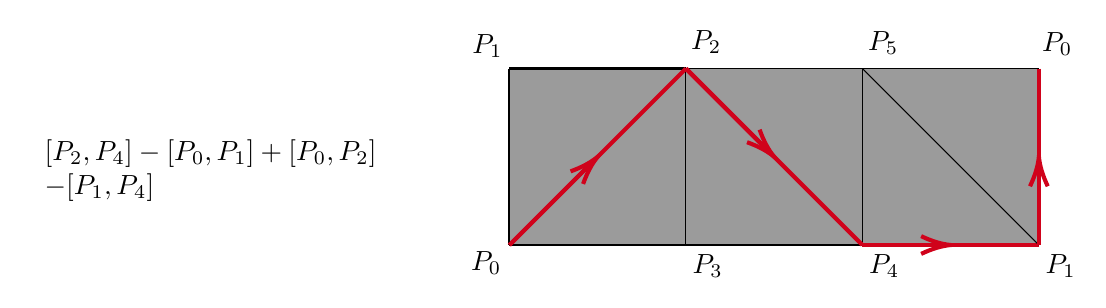
\begin{tikzpicture}[x=0.75pt,y=0.75pt,yscale=-1,xscale=1]
        %uncomment if require: \path (0,735); %set diagram left start at 0, and has height of 735

        %Shape: Polygon [id:ds012901580416037284] 
        \draw  [fill={rgb, 255:red, 155; green, 155; blue, 155 }  ,fill opacity=1 ] (510.43,41.9) -- (510.43,126.93) -- (255.35,126.93) -- (255.35,41.9) -- cycle ;
        %Straight Lines [id:da7117464125713011] 
        \draw [color={rgb, 255:red, 0; green, 0; blue, 0 }  ,draw opacity=1 ][line width=0.75]    (255.35,41.9) -- (340.37,41.9) ;
        %Straight Lines [id:da8593345105117205] 
        \draw    (340.37,41.9) -- (425.4,41.9) ;
        %Straight Lines [id:da3706532081604941] 
        \draw    (425.4,41.9) -- (510.43,41.9) ;
        %Straight Lines [id:da5527262236568335] 
        \draw    (255.35,126.93) -- (340.37,126.93) ;
        %Straight Lines [id:da6652833889288519] 
        \draw    (340.37,126.93) -- (425.4,126.93) ;
        %Straight Lines [id:da2635536835037924] 
        \draw [color={rgb, 255:red, 208; green, 2; blue, 27 }  ,draw opacity=1 ][line width=1.5]    (425.4,126.93) -- (510.43,126.93) ;
        %Straight Lines [id:da7627774994062366] 
        \draw [color={rgb, 255:red, 0; green, 0; blue, 0 }  ,draw opacity=1 ][line width=0.75]    (255.35,41.9) -- (255.35,126.93) ;
        %Straight Lines [id:da5611032436091536] 
        \draw    (340.37,41.9) -- (340.37,126.93) ;
        %Straight Lines [id:da5168532258652223] 
        \draw    (425.4,41.9) -- (425.4,126.93) ;
        %Straight Lines [id:da6975191425087921] 
        \draw [color={rgb, 255:red, 208; green, 2; blue, 27 }  ,draw opacity=1 ][line width=1.5]    (510.43,41.9) -- (510.43,126.93) ;
        %Straight Lines [id:da7664706882169221] 
        \draw [color={rgb, 255:red, 208; green, 2; blue, 27 }  ,draw opacity=1 ][line width=1.5]    (340.37,41.9) -- (255.35,126.93) ;
        %Straight Lines [id:da7670217078686072] 
        \draw [color={rgb, 255:red, 208; green, 2; blue, 27 }  ,draw opacity=1 ][line width=1.5]    (425.4,126.93) -- (340.37,41.9) ;
        %Straight Lines [id:da32965091603665986] 
        \draw    (510.43,126.93) -- (425.4,41.9) ;
        %Straight Lines [id:da14826879708125862] 
        \draw [color={rgb, 255:red, 208; green, 2; blue, 27 }  ,draw opacity=1 ][line width=1.5]    (340.37,41.9) -- (380.76,82.29) ;
        \draw [shift={(382.89,84.42)}, rotate = 225] [color={rgb, 255:red, 208; green, 2; blue, 27 }  ,draw opacity=1 ][line width=1.5]    (14.21,-4.28) .. controls (9.04,-1.82) and (4.3,-0.39) .. (0,0) .. controls (4.3,0.39) and (9.04,1.82) .. (14.21,4.28)   ;
        %Straight Lines [id:da045805197883367565] 
        \draw [color={rgb, 255:red, 208; green, 2; blue, 27 }  ,draw opacity=1 ][line width=1.5]    (255.35,126.93) -- (295.74,86.54) ;
        \draw [shift={(297.86,84.42)}, rotate = 135] [color={rgb, 255:red, 208; green, 2; blue, 27 }  ,draw opacity=1 ][line width=1.5]    (14.21,-4.28) .. controls (9.04,-1.82) and (4.3,-0.39) .. (0,0) .. controls (4.3,0.39) and (9.04,1.82) .. (14.21,4.28)   ;
        %Straight Lines [id:da2589861639102189] 
        \draw [color={rgb, 255:red, 208; green, 2; blue, 27 }  ,draw opacity=1 ][line width=1.5]    (425.4,126.93) -- (464.91,126.93) ;
        \draw [shift={(467.91,126.93)}, rotate = 180] [color={rgb, 255:red, 208; green, 2; blue, 27 }  ,draw opacity=1 ][line width=1.5]    (14.21,-4.28) .. controls (9.04,-1.82) and (4.3,-0.39) .. (0,0) .. controls (4.3,0.39) and (9.04,1.82) .. (14.21,4.28)   ;
        %Straight Lines [id:da8424442933971612] 
        \draw [color={rgb, 255:red, 208; green, 2; blue, 27 }  ,draw opacity=1 ][line width=1.5]    (510.43,126.93) -- (510.43,87.42) ;
        \draw [shift={(510.43,84.42)}, rotate = 90] [color={rgb, 255:red, 208; green, 2; blue, 27 }  ,draw opacity=1 ][line width=1.5]    (14.21,-4.28) .. controls (9.04,-1.82) and (4.3,-0.39) .. (0,0) .. controls (4.3,0.39) and (9.04,1.82) .. (14.21,4.28)   ;

        % Text Node
        \draw (235.63,128.85) node [anchor=north west][inner sep=0.75pt]    {$P_{0}$};
        % Text Node
        \draw (510.73,23.11) node [anchor=north west][inner sep=0.75pt]    {$P_{0}$};
        % Text Node
        \draw (236.24,24.05) node [anchor=north west][inner sep=0.75pt]    {$P_{1}$};
        % Text Node
        \draw (512.43,130.33) node [anchor=north west][inner sep=0.75pt]    {$P_{1}$};
        % Text Node
        \draw (342.37,130.33) node [anchor=north west][inner sep=0.75pt]    {$P_{3}$};
        % Text Node
        \draw (341.62,22.48) node [anchor=north west][inner sep=0.75pt]    {$P_{2}$};
        % Text Node
        \draw (427.4,130.33) node [anchor=north west][inner sep=0.75pt]    {$P_{4}$};
        % Text Node
        \draw (426.86,22.7) node [anchor=north west][inner sep=0.75pt]    {$P_{5}$};
        % Text Node
        \draw (23.5,73.9) node [anchor=north west][inner sep=0.75pt]    {$ \begin{array}{l}
                    [ P_{2} ,P_{4}] -[ P_{0} ,P_{1}] +[ P_{0} ,P_{2}] \\
                    -[ P_{1} ,P_{4}]
                \end{array}$};


    \end{tikzpicture}

\end{center}
\begin{center}


    \tikzset{every picture/.style={line width=0.75pt}} %set default line width to 0.75pt        

    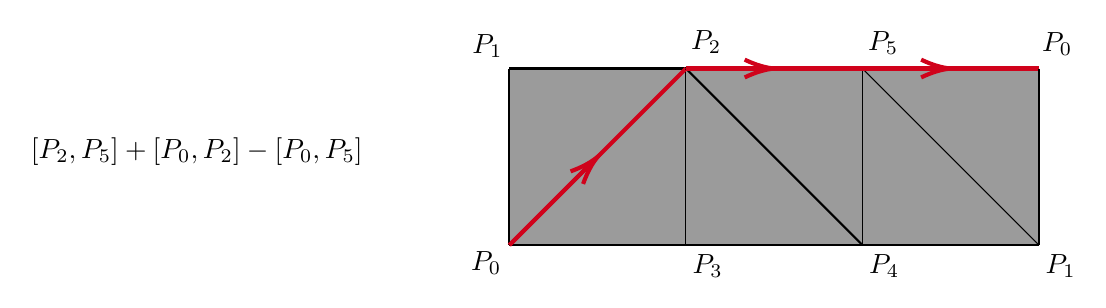
\begin{tikzpicture}[x=0.75pt,y=0.75pt,yscale=-1,xscale=1]
        %uncomment if require: \path (0,735); %set diagram left start at 0, and has height of 735

        %Shape: Polygon [id:ds012901580416037284] 
        \draw  [fill={rgb, 255:red, 155; green, 155; blue, 155 }  ,fill opacity=1 ] (510.43,41.9) -- (510.43,126.93) -- (255.35,126.93) -- (255.35,41.9) -- cycle ;
        %Straight Lines [id:da7117464125713011] 
        \draw [color={rgb, 255:red, 0; green, 0; blue, 0 }  ,draw opacity=1 ][line width=0.75]    (255.35,41.9) -- (340.37,41.9) ;
        %Straight Lines [id:da8593345105117205] 
        \draw [color={rgb, 255:red, 208; green, 2; blue, 27 }  ,draw opacity=1 ][line width=1.5]    (340.37,41.9) -- (425.4,41.9) ;
        %Straight Lines [id:da3706532081604941] 
        \draw [color={rgb, 255:red, 208; green, 2; blue, 27 }  ,draw opacity=1 ][line width=1.5]    (425.4,41.9) -- (510.43,41.9) ;
        %Straight Lines [id:da5527262236568335] 
        \draw    (255.35,126.93) -- (340.37,126.93) ;
        %Straight Lines [id:da6652833889288519] 
        \draw    (340.37,126.93) -- (425.4,126.93) ;
        %Straight Lines [id:da2635536835037924] 
        \draw [color={rgb, 255:red, 0; green, 0; blue, 0 }  ,draw opacity=1 ][line width=0.75]    (425.4,126.93) -- (510.43,126.93) ;
        %Straight Lines [id:da7627774994062366] 
        \draw [color={rgb, 255:red, 0; green, 0; blue, 0 }  ,draw opacity=1 ][line width=0.75]    (255.35,41.9) -- (255.35,126.93) ;
        %Straight Lines [id:da5611032436091536] 
        \draw    (340.37,41.9) -- (340.37,126.93) ;
        %Straight Lines [id:da5168532258652223] 
        \draw    (425.4,41.9) -- (425.4,126.93) ;
        %Straight Lines [id:da6975191425087921] 
        \draw [color={rgb, 255:red, 0; green, 0; blue, 0 }  ,draw opacity=1 ][line width=0.75]    (510.43,41.9) -- (510.43,126.93) ;
        %Straight Lines [id:da7664706882169221] 
        \draw [color={rgb, 255:red, 208; green, 2; blue, 27 }  ,draw opacity=1 ][line width=1.5]    (340.37,41.9) -- (255.35,126.93) ;
        %Straight Lines [id:da7670217078686072] 
        \draw [color={rgb, 255:red, 0; green, 0; blue, 0 }  ,draw opacity=1 ][line width=0.75]    (425.4,126.93) -- (340.37,41.9) ;
        %Straight Lines [id:da32965091603665986] 
        \draw    (510.43,126.93) -- (425.4,41.9) ;
        %Straight Lines [id:da14826879708125862] 
        \draw [color={rgb, 255:red, 208; green, 2; blue, 27 }  ,draw opacity=1 ][line width=1.5]    (340.37,41.9) -- (379.89,41.9) ;
        \draw [shift={(382.89,41.9)}, rotate = 180] [color={rgb, 255:red, 208; green, 2; blue, 27 }  ,draw opacity=1 ][line width=1.5]    (14.21,-4.28) .. controls (9.04,-1.82) and (4.3,-0.39) .. (0,0) .. controls (4.3,0.39) and (9.04,1.82) .. (14.21,4.28)   ;
        %Straight Lines [id:da045805197883367565] 
        \draw [color={rgb, 255:red, 208; green, 2; blue, 27 }  ,draw opacity=1 ][line width=1.5]    (255.35,126.93) -- (295.74,86.54) ;
        \draw [shift={(297.86,84.42)}, rotate = 135] [color={rgb, 255:red, 208; green, 2; blue, 27 }  ,draw opacity=1 ][line width=1.5]    (14.21,-4.28) .. controls (9.04,-1.82) and (4.3,-0.39) .. (0,0) .. controls (4.3,0.39) and (9.04,1.82) .. (14.21,4.28)   ;
        %Straight Lines [id:da2589861639102189] 
        \draw [color={rgb, 255:red, 208; green, 2; blue, 27 }  ,draw opacity=1 ][line width=1.5]    (425.4,41.9) -- (464.91,41.9) ;
        \draw [shift={(467.91,41.9)}, rotate = 180] [color={rgb, 255:red, 208; green, 2; blue, 27 }  ,draw opacity=1 ][line width=1.5]    (14.21,-4.28) .. controls (9.04,-1.82) and (4.3,-0.39) .. (0,0) .. controls (4.3,0.39) and (9.04,1.82) .. (14.21,4.28)   ;

        % Text Node
        \draw (235.63,128.85) node [anchor=north west][inner sep=0.75pt]    {$P_{0}$};
        % Text Node
        \draw (510.73,23.11) node [anchor=north west][inner sep=0.75pt]    {$P_{0}$};
        % Text Node
        \draw (236.24,24.05) node [anchor=north west][inner sep=0.75pt]    {$P_{1}$};
        % Text Node
        \draw (512.43,130.33) node [anchor=north west][inner sep=0.75pt]    {$P_{1}$};
        % Text Node
        \draw (342.37,130.33) node [anchor=north west][inner sep=0.75pt]    {$P_{3}$};
        % Text Node
        \draw (341.62,22.48) node [anchor=north west][inner sep=0.75pt]    {$P_{2}$};
        % Text Node
        \draw (427.4,130.33) node [anchor=north west][inner sep=0.75pt]    {$P_{4}$};
        % Text Node
        \draw (426.86,22.7) node [anchor=north west][inner sep=0.75pt]    {$P_{5}$};
        % Text Node
        \draw (23.5,73.9) node [anchor=north west][inner sep=0.75pt]    {$[ P_{2} ,P_{5}] +[ P_{0} ,P_{2}] -[ P_{0} ,P_{5}]$};


    \end{tikzpicture}

\end{center}
\begin{center}


    \tikzset{every picture/.style={line width=0.75pt}} %set default line width to 0.75pt        

    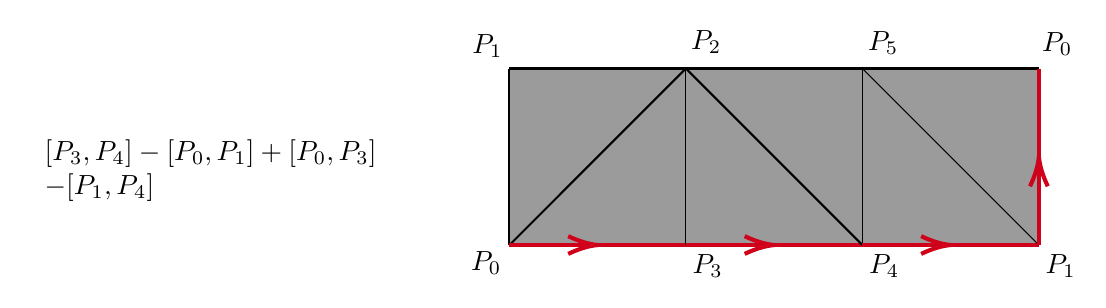
\begin{tikzpicture}[x=0.75pt,y=0.75pt,yscale=-1,xscale=1]
        %uncomment if require: \path (0,735); %set diagram left start at 0, and has height of 735

        %Shape: Polygon [id:ds012901580416037284] 
        \draw  [fill={rgb, 255:red, 155; green, 155; blue, 155 }  ,fill opacity=1 ] (510.43,41.9) -- (510.43,126.93) -- (255.35,126.93) -- (255.35,41.9) -- cycle ;
        %Straight Lines [id:da7117464125713011] 
        \draw [color={rgb, 255:red, 0; green, 0; blue, 0 }  ,draw opacity=1 ][line width=0.75]    (255.35,41.9) -- (340.37,41.9) ;
        %Straight Lines [id:da8593345105117205] 
        \draw [color={rgb, 255:red, 0; green, 0; blue, 0 }  ,draw opacity=1 ][line width=0.75]    (340.37,41.9) -- (425.4,41.9) ;
        %Straight Lines [id:da3706532081604941] 
        \draw [color={rgb, 255:red, 0; green, 0; blue, 0 }  ,draw opacity=1 ][line width=0.75]    (425.4,41.9) -- (510.43,41.9) ;
        %Straight Lines [id:da5527262236568335] 
        \draw [color={rgb, 255:red, 208; green, 2; blue, 27 }  ,draw opacity=1 ][line width=1.5]    (255.35,126.93) -- (340.37,126.93) ;
        %Straight Lines [id:da6652833889288519] 
        \draw [color={rgb, 255:red, 208; green, 2; blue, 27 }  ,draw opacity=1 ][line width=1.5]    (340.37,126.93) -- (425.4,126.93) ;
        %Straight Lines [id:da2635536835037924] 
        \draw [color={rgb, 255:red, 208; green, 2; blue, 27 }  ,draw opacity=1 ][line width=1.5]    (425.4,126.93) -- (510.43,126.93) ;
        %Straight Lines [id:da7627774994062366] 
        \draw [color={rgb, 255:red, 0; green, 0; blue, 0 }  ,draw opacity=1 ][line width=0.75]    (255.35,41.9) -- (255.35,126.93) ;
        %Straight Lines [id:da5611032436091536] 
        \draw    (340.37,41.9) -- (340.37,126.93) ;
        %Straight Lines [id:da5168532258652223] 
        \draw    (425.4,41.9) -- (425.4,126.93) ;
        %Straight Lines [id:da6975191425087921] 
        \draw [color={rgb, 255:red, 208; green, 2; blue, 27 }  ,draw opacity=1 ][line width=1.5]    (510.43,41.9) -- (510.43,126.93) ;
        %Straight Lines [id:da7664706882169221] 
        \draw [color={rgb, 255:red, 0; green, 0; blue, 0 }  ,draw opacity=1 ][line width=0.75]    (340.37,41.9) -- (255.35,126.93) ;
        %Straight Lines [id:da7670217078686072] 
        \draw [color={rgb, 255:red, 0; green, 0; blue, 0 }  ,draw opacity=1 ][line width=0.75]    (425.4,126.93) -- (340.37,41.9) ;
        %Straight Lines [id:da32965091603665986] 
        \draw    (510.43,126.93) -- (425.4,41.9) ;
        %Straight Lines [id:da14826879708125862] 
        \draw [color={rgb, 255:red, 208; green, 2; blue, 27 }  ,draw opacity=1 ][line width=1.5]    (340.37,126.93) -- (379.89,126.93) ;
        \draw [shift={(382.89,126.93)}, rotate = 180] [color={rgb, 255:red, 208; green, 2; blue, 27 }  ,draw opacity=1 ][line width=1.5]    (14.21,-4.28) .. controls (9.04,-1.82) and (4.3,-0.39) .. (0,0) .. controls (4.3,0.39) and (9.04,1.82) .. (14.21,4.28)   ;
        %Straight Lines [id:da045805197883367565] 
        \draw [color={rgb, 255:red, 208; green, 2; blue, 27 }  ,draw opacity=1 ][line width=1.5]    (510.43,126.93) -- (510.43,87.42) ;
        \draw [shift={(510.43,84.42)}, rotate = 90] [color={rgb, 255:red, 208; green, 2; blue, 27 }  ,draw opacity=1 ][line width=1.5]    (14.21,-4.28) .. controls (9.04,-1.82) and (4.3,-0.39) .. (0,0) .. controls (4.3,0.39) and (9.04,1.82) .. (14.21,4.28)   ;
        %Straight Lines [id:da2589861639102189] 
        \draw [color={rgb, 255:red, 208; green, 2; blue, 27 }  ,draw opacity=1 ][line width=1.5]    (425.4,126.93) -- (464.91,126.93) ;
        \draw [shift={(467.91,126.93)}, rotate = 180] [color={rgb, 255:red, 208; green, 2; blue, 27 }  ,draw opacity=1 ][line width=1.5]    (14.21,-4.28) .. controls (9.04,-1.82) and (4.3,-0.39) .. (0,0) .. controls (4.3,0.39) and (9.04,1.82) .. (14.21,4.28)   ;
        %Straight Lines [id:da5086511388616413] 
        \draw [color={rgb, 255:red, 208; green, 2; blue, 27 }  ,draw opacity=1 ][line width=1.5]    (255.35,126.93) -- (294.86,126.93) ;
        \draw [shift={(297.86,126.93)}, rotate = 180] [color={rgb, 255:red, 208; green, 2; blue, 27 }  ,draw opacity=1 ][line width=1.5]    (14.21,-4.28) .. controls (9.04,-1.82) and (4.3,-0.39) .. (0,0) .. controls (4.3,0.39) and (9.04,1.82) .. (14.21,4.28)   ;

        % Text Node
        \draw (235.63,128.85) node [anchor=north west][inner sep=0.75pt]    {$P_{0}$};
        % Text Node
        \draw (510.73,23.11) node [anchor=north west][inner sep=0.75pt]    {$P_{0}$};
        % Text Node
        \draw (236.24,24.05) node [anchor=north west][inner sep=0.75pt]    {$P_{1}$};
        % Text Node
        \draw (512.43,130.33) node [anchor=north west][inner sep=0.75pt]    {$P_{1}$};
        % Text Node
        \draw (342.37,130.33) node [anchor=north west][inner sep=0.75pt]    {$P_{3}$};
        % Text Node
        \draw (341.62,22.48) node [anchor=north west][inner sep=0.75pt]    {$P_{2}$};
        % Text Node
        \draw (427.4,130.33) node [anchor=north west][inner sep=0.75pt]    {$P_{4}$};
        % Text Node
        \draw (426.86,22.7) node [anchor=north west][inner sep=0.75pt]    {$P_{5}$};
        % Text Node
        \draw (23.5,73.9) node [anchor=north west][inner sep=0.75pt]    {$ \begin{array}{l}
                    [ P_{3} ,P_{4}] -[ P_{0} ,P_{1}] +[ P_{0} ,P_{3}] \\
                    -[ P_{1} ,P_{4}]
                \end{array}$};


    \end{tikzpicture}

\end{center}
\begin{center}


    \tikzset{every picture/.style={line width=0.75pt}} %set default line width to 0.75pt        

    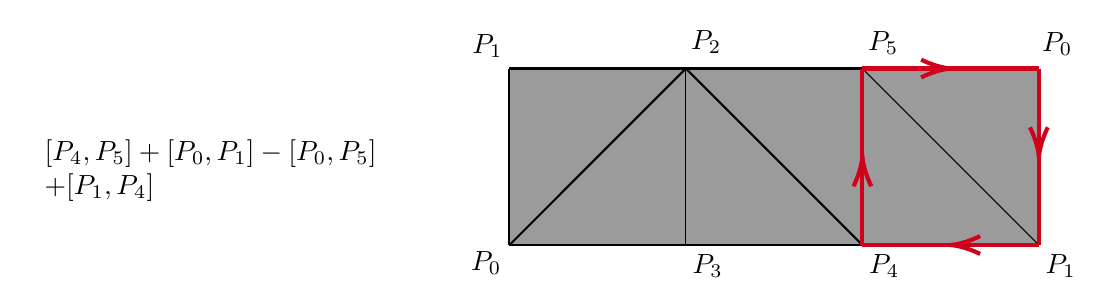
\begin{tikzpicture}[x=0.75pt,y=0.75pt,yscale=-1,xscale=1]
        %uncomment if require: \path (0,735); %set diagram left start at 0, and has height of 735

        %Shape: Polygon [id:ds012901580416037284] 
        \draw  [fill={rgb, 255:red, 155; green, 155; blue, 155 }  ,fill opacity=1 ] (510.43,41.9) -- (510.43,126.93) -- (255.35,126.93) -- (255.35,41.9) -- cycle ;
        %Straight Lines [id:da7117464125713011] 
        \draw [color={rgb, 255:red, 0; green, 0; blue, 0 }  ,draw opacity=1 ][line width=0.75]    (255.35,41.9) -- (340.37,41.9) ;
        %Straight Lines [id:da8593345105117205] 
        \draw [color={rgb, 255:red, 0; green, 0; blue, 0 }  ,draw opacity=1 ][line width=0.75]    (340.37,41.9) -- (425.4,41.9) ;
        %Straight Lines [id:da3706532081604941] 
        \draw [color={rgb, 255:red, 208; green, 2; blue, 27 }  ,draw opacity=1 ][line width=1.5]    (425.4,41.9) -- (510.43,41.9) ;
        %Straight Lines [id:da5527262236568335] 
        \draw [color={rgb, 255:red, 0; green, 0; blue, 0 }  ,draw opacity=1 ][line width=0.75]    (255.35,126.93) -- (340.37,126.93) ;
        %Straight Lines [id:da6652833889288519] 
        \draw [color={rgb, 255:red, 0; green, 0; blue, 0 }  ,draw opacity=1 ][line width=0.75]    (340.37,126.93) -- (425.4,126.93) ;
        %Straight Lines [id:da2635536835037924] 
        \draw [color={rgb, 255:red, 208; green, 2; blue, 27 }  ,draw opacity=1 ][line width=1.5]    (425.4,126.93) -- (510.43,126.93) ;
        %Straight Lines [id:da7627774994062366] 
        \draw [color={rgb, 255:red, 0; green, 0; blue, 0 }  ,draw opacity=1 ][line width=0.75]    (255.35,41.9) -- (255.35,126.93) ;
        %Straight Lines [id:da5611032436091536] 
        \draw    (340.37,41.9) -- (340.37,126.93) ;
        %Straight Lines [id:da5168532258652223] 
        \draw [color={rgb, 255:red, 208; green, 2; blue, 27 }  ,draw opacity=1 ][line width=1.5]    (425.4,41.9) -- (425.4,126.93) ;
        %Straight Lines [id:da6975191425087921] 
        \draw [color={rgb, 255:red, 208; green, 2; blue, 27 }  ,draw opacity=1 ][line width=1.5]    (510.43,41.9) -- (510.43,126.93) ;
        %Straight Lines [id:da7664706882169221] 
        \draw [color={rgb, 255:red, 0; green, 0; blue, 0 }  ,draw opacity=1 ][line width=0.75]    (340.37,41.9) -- (255.35,126.93) ;
        %Straight Lines [id:da7670217078686072] 
        \draw [color={rgb, 255:red, 0; green, 0; blue, 0 }  ,draw opacity=1 ][line width=0.75]    (425.4,126.93) -- (340.37,41.9) ;
        %Straight Lines [id:da32965091603665986] 
        \draw    (510.43,126.93) -- (425.4,41.9) ;
        %Straight Lines [id:da14826879708125862] 
        \draw [color={rgb, 255:red, 208; green, 2; blue, 27 }  ,draw opacity=1 ][line width=1.5]    (425.4,41.9) -- (464.91,41.9) ;
        \draw [shift={(467.91,41.9)}, rotate = 180] [color={rgb, 255:red, 208; green, 2; blue, 27 }  ,draw opacity=1 ][line width=1.5]    (14.21,-4.28) .. controls (9.04,-1.82) and (4.3,-0.39) .. (0,0) .. controls (4.3,0.39) and (9.04,1.82) .. (14.21,4.28)   ;
        %Straight Lines [id:da045805197883367565] 
        \draw [color={rgb, 255:red, 208; green, 2; blue, 27 }  ,draw opacity=1 ][line width=1.5]    (510.43,41.9) -- (510.43,81.42) ;
        \draw [shift={(510.43,84.42)}, rotate = 270] [color={rgb, 255:red, 208; green, 2; blue, 27 }  ,draw opacity=1 ][line width=1.5]    (14.21,-4.28) .. controls (9.04,-1.82) and (4.3,-0.39) .. (0,0) .. controls (4.3,0.39) and (9.04,1.82) .. (14.21,4.28)   ;
        %Straight Lines [id:da2589861639102189] 
        \draw [color={rgb, 255:red, 208; green, 2; blue, 27 }  ,draw opacity=1 ][line width=1.5]    (510.43,126.93) -- (470.91,126.93) ;
        \draw [shift={(467.91,126.93)}, rotate = 360] [color={rgb, 255:red, 208; green, 2; blue, 27 }  ,draw opacity=1 ][line width=1.5]    (14.21,-4.28) .. controls (9.04,-1.82) and (4.3,-0.39) .. (0,0) .. controls (4.3,0.39) and (9.04,1.82) .. (14.21,4.28)   ;
        %Straight Lines [id:da5429429554252891] 
        \draw [color={rgb, 255:red, 208; green, 2; blue, 27 }  ,draw opacity=1 ][line width=1.5]    (425.4,126.93) -- (425.4,87.42) ;
        \draw [shift={(425.4,84.42)}, rotate = 90] [color={rgb, 255:red, 208; green, 2; blue, 27 }  ,draw opacity=1 ][line width=1.5]    (14.21,-4.28) .. controls (9.04,-1.82) and (4.3,-0.39) .. (0,0) .. controls (4.3,0.39) and (9.04,1.82) .. (14.21,4.28)   ;

        % Text Node
        \draw (235.63,128.85) node [anchor=north west][inner sep=0.75pt]    {$P_{0}$};
        % Text Node
        \draw (510.73,23.11) node [anchor=north west][inner sep=0.75pt]    {$P_{0}$};
        % Text Node
        \draw (236.24,24.05) node [anchor=north west][inner sep=0.75pt]    {$P_{1}$};
        % Text Node
        \draw (512.43,130.33) node [anchor=north west][inner sep=0.75pt]    {$P_{1}$};
        % Text Node
        \draw (342.37,130.33) node [anchor=north west][inner sep=0.75pt]    {$P_{3}$};
        % Text Node
        \draw (341.62,22.48) node [anchor=north west][inner sep=0.75pt]    {$P_{2}$};
        % Text Node
        \draw (427.4,130.33) node [anchor=north west][inner sep=0.75pt]    {$P_{4}$};
        % Text Node
        \draw (426.86,22.7) node [anchor=north west][inner sep=0.75pt]    {$P_{5}$};
        % Text Node
        \draw (23.5,73.9) node [anchor=north west][inner sep=0.75pt]    {$ \begin{array}{l}
                    [ P_{4} ,P_{5}] +[ P_{0} ,P_{1}] -[ P_{0} ,P_{5}] \\
                    +[ P_{1} ,P_{4}]
                \end{array}$};


    \end{tikzpicture}

\end{center}
Riepilogo:
\[
    H_2(M)=Ker\ \partial_2=\{0\}
\]
\[
    H_1(M)=\gen{P_0}\simeq\Z\quad\text{(prevedibile, dato che $|M|$ è connesso)}
\]
\[
    H_0(M)=\faktor{Ker\ \partial_1}{Im\ \partial_2}=\faktor{Z_1(M)}{B_1(M)}\simeq\faktor{\Z^7}{\Z^6}
\]
\paragraph{Osservazione} Ho 6 bordi provenienti dai 2-simplessi di $M$, tuttavia
\[
    Z_1(M)\simeq\Z^7
\]
ho quindi un 1-ciclo che non proviene da una 2-catena mediante $\partial_2$\\
I tre cammini chiusi da $P_0$ a $P_0$
\[
    [P_2,P_4]-[P_0,P_1]+[P_0,P_2]-[P_1,P_4]
\]
\[
    [P_2,P_5]+[P_0,P_2]-[P_0,P_5]
\]
\[
    [P_3,P_4]-[P_0,P_1]+[P_0,P_3]-[P_1,P_4]
\]
differiscono per un elemento nel sottogruppo degli 1-bordi, non sono quindi indipendenti nel gruppo $H_1(M)$
\[
    ([P_2,P_4]-[P_0,P_1]+[P_0,P_2]-[P_1,P_4])-([P_2,P_5]+[P_0,P_2]-[P_0,P_5])=
\]
\[
    =-[P_0,P_1]+[P_0,P_5]-[P_1,P_4]+[P_2,P_4]-[P_2,P_5]\in B_1(M)
\]
\begin{center}


    \tikzset{every picture/.style={line width=0.75pt}} %set default line width to 0.75pt        

    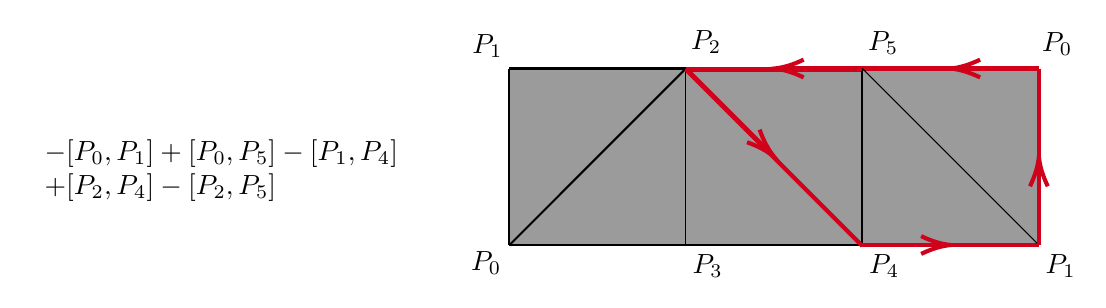
\begin{tikzpicture}[x=0.75pt,y=0.75pt,yscale=-1,xscale=1]
        %uncomment if require: \path (0,735); %set diagram left start at 0, and has height of 735

        %Shape: Polygon [id:ds012901580416037284] 
        \draw  [fill={rgb, 255:red, 155; green, 155; blue, 155 }  ,fill opacity=1 ] (510.43,41.9) -- (510.43,126.93) -- (255.35,126.93) -- (255.35,41.9) -- cycle ;
        %Straight Lines [id:da7117464125713011] 
        \draw [color={rgb, 255:red, 0; green, 0; blue, 0 }  ,draw opacity=1 ][line width=0.75]    (255.35,41.9) -- (340.37,41.9) ;
        %Straight Lines [id:da8593345105117205] 
        \draw [color={rgb, 255:red, 208; green, 2; blue, 27 }  ,draw opacity=1 ][line width=1.5]    (340.37,42.4) -- (425.4,42.4) ;
        %Straight Lines [id:da3706532081604941] 
        \draw [color={rgb, 255:red, 208; green, 2; blue, 27 }  ,draw opacity=1 ][line width=1.5]    (425.4,41.9) -- (510.43,41.9) ;
        %Straight Lines [id:da5527262236568335] 
        \draw [color={rgb, 255:red, 0; green, 0; blue, 0 }  ,draw opacity=1 ][line width=0.75]    (255.35,126.93) -- (340.37,126.93) ;
        %Straight Lines [id:da6652833889288519] 
        \draw [color={rgb, 255:red, 0; green, 0; blue, 0 }  ,draw opacity=1 ][line width=0.75]    (340.37,126.93) -- (425.4,126.93) ;
        %Straight Lines [id:da2635536835037924] 
        \draw [color={rgb, 255:red, 208; green, 2; blue, 27 }  ,draw opacity=1 ][line width=1.5]    (425.4,126.93) -- (510.43,126.93) ;
        %Straight Lines [id:da7627774994062366] 
        \draw [color={rgb, 255:red, 0; green, 0; blue, 0 }  ,draw opacity=1 ][line width=0.75]    (255.35,41.9) -- (255.35,126.93) ;
        %Straight Lines [id:da5611032436091536] 
        \draw    (340.37,41.9) -- (340.37,126.93) ;
        %Straight Lines [id:da5168532258652223] 
        \draw [color={rgb, 255:red, 0; green, 0; blue, 0 }  ,draw opacity=1 ][line width=0.75]    (425.4,41.9) -- (425.4,126.93) ;
        %Straight Lines [id:da6975191425087921] 
        \draw [color={rgb, 255:red, 208; green, 2; blue, 27 }  ,draw opacity=1 ][line width=1.5]    (510.43,41.9) -- (510.43,126.93) ;
        %Straight Lines [id:da7664706882169221] 
        \draw [color={rgb, 255:red, 0; green, 0; blue, 0 }  ,draw opacity=1 ][line width=0.75]    (340.37,41.9) -- (255.35,126.93) ;
        %Straight Lines [id:da7670217078686072] 
        \draw [color={rgb, 255:red, 208; green, 2; blue, 27 }  ,draw opacity=1 ][line width=1.5]    (425.4,127.43) -- (340.37,42.4) ;
        %Straight Lines [id:da32965091603665986] 
        \draw    (510.43,126.93) -- (425.4,41.9) ;
        %Straight Lines [id:da14826879708125862] 
        \draw [color={rgb, 255:red, 208; green, 2; blue, 27 }  ,draw opacity=1 ][line width=1.5]    (510.43,41.9) -- (470.91,41.9) ;
        \draw [shift={(467.91,41.9)}, rotate = 360] [color={rgb, 255:red, 208; green, 2; blue, 27 }  ,draw opacity=1 ][line width=1.5]    (14.21,-4.28) .. controls (9.04,-1.82) and (4.3,-0.39) .. (0,0) .. controls (4.3,0.39) and (9.04,1.82) .. (14.21,4.28)   ;
        %Straight Lines [id:da045805197883367565] 
        \draw [color={rgb, 255:red, 208; green, 2; blue, 27 }  ,draw opacity=1 ][line width=1.5]    (510.43,126.93) -- (510.43,87.42) ;
        \draw [shift={(510.43,84.42)}, rotate = 90] [color={rgb, 255:red, 208; green, 2; blue, 27 }  ,draw opacity=1 ][line width=1.5]    (14.21,-4.28) .. controls (9.04,-1.82) and (4.3,-0.39) .. (0,0) .. controls (4.3,0.39) and (9.04,1.82) .. (14.21,4.28)   ;
        %Straight Lines [id:da2589861639102189] 
        \draw [color={rgb, 255:red, 208; green, 2; blue, 27 }  ,draw opacity=1 ][line width=1.5]    (425.4,126.93) -- (464.91,126.93) ;
        \draw [shift={(467.91,126.93)}, rotate = 180] [color={rgb, 255:red, 208; green, 2; blue, 27 }  ,draw opacity=1 ][line width=1.5]    (14.21,-4.28) .. controls (9.04,-1.82) and (4.3,-0.39) .. (0,0) .. controls (4.3,0.39) and (9.04,1.82) .. (14.21,4.28)   ;
        %Straight Lines [id:da5429429554252891] 
        \draw [color={rgb, 255:red, 208; green, 2; blue, 27 }  ,draw opacity=1 ][line width=1.5]    (340.37,41.9) -- (380.76,82.29) ;
        \draw [shift={(382.89,84.42)}, rotate = 225] [color={rgb, 255:red, 208; green, 2; blue, 27 }  ,draw opacity=1 ][line width=1.5]    (14.21,-4.28) .. controls (9.04,-1.82) and (4.3,-0.39) .. (0,0) .. controls (4.3,0.39) and (9.04,1.82) .. (14.21,4.28)   ;
        %Straight Lines [id:da29481019269701325] 
        \draw [color={rgb, 255:red, 208; green, 2; blue, 27 }  ,draw opacity=1 ][line width=1.5]    (425.4,41.9) -- (385.89,41.9) ;
        \draw [shift={(382.89,41.9)}, rotate = 360] [color={rgb, 255:red, 208; green, 2; blue, 27 }  ,draw opacity=1 ][line width=1.5]    (14.21,-4.28) .. controls (9.04,-1.82) and (4.3,-0.39) .. (0,0) .. controls (4.3,0.39) and (9.04,1.82) .. (14.21,4.28)   ;

        % Text Node
        \draw (235.63,128.85) node [anchor=north west][inner sep=0.75pt]    {$P_{0}$};
        % Text Node
        \draw (510.73,23.11) node [anchor=north west][inner sep=0.75pt]    {$P_{0}$};
        % Text Node
        \draw (236.24,24.05) node [anchor=north west][inner sep=0.75pt]    {$P_{1}$};
        % Text Node
        \draw (512.43,130.33) node [anchor=north west][inner sep=0.75pt]    {$P_{1}$};
        % Text Node
        \draw (342.37,130.33) node [anchor=north west][inner sep=0.75pt]    {$P_{3}$};
        % Text Node
        \draw (341.62,22.48) node [anchor=north west][inner sep=0.75pt]    {$P_{2}$};
        % Text Node
        \draw (427.4,130.33) node [anchor=north west][inner sep=0.75pt]    {$P_{4}$};
        % Text Node
        \draw (426.86,22.7) node [anchor=north west][inner sep=0.75pt]    {$P_{5}$};
        % Text Node
        \draw (23.5,73.9) node [anchor=north west][inner sep=0.75pt]    {$ \begin{array}{l}
                    -[ P_{0} ,P_{1}] +[ P_{0} ,P_{5}] -[ P_{1} ,P_{4}] \\
                    +[ P_{2} ,P_{4}] -[ P_{2} ,P_{5}]
                \end{array}$};


    \end{tikzpicture}

\end{center}
\[
    ([P_2,P_5]+[P_0,P_2]-[P_0,P_5])-([P_3,P_4]-[P_0,P_1]+[P_0,P_3]-[P_1,P_4])=
\]
\[
    [P_2,P_5]+[P_0,P_2]-[P_0,P_5]-[P_3,P_4]+[P_0,P_1]-[P_0,P_3]+[P_1,P_4]\in B_1(M)
\]
\begin{center}


    \tikzset{every picture/.style={line width=0.75pt}} %set default line width to 0.75pt        

    \begin{tikzpicture}[x=0.75pt,y=0.75pt,yscale=-1,xscale=1]
        %uncomment if require: \path (0,735); %set diagram left start at 0, and has height of 735

        %Shape: Polygon [id:ds012901580416037284] 
        \draw  [fill={rgb, 255:red, 155; green, 155; blue, 155 }  ,fill opacity=1 ] (510.43,41.9) -- (510.43,126.93) -- (255.35,126.93) -- (255.35,41.9) -- cycle ;
        %Straight Lines [id:da7117464125713011] 
        \draw [color={rgb, 255:red, 0; green, 0; blue, 0 }  ,draw opacity=1 ][line width=0.75]    (255.35,41.9) -- (340.37,41.9) ;
        %Straight Lines [id:da8593345105117205] 
        \draw [color={rgb, 255:red, 208; green, 2; blue, 27 }  ,draw opacity=1 ][line width=1.5]    (340.37,42.4) -- (425.4,42.4) ;
        %Straight Lines [id:da3706532081604941] 
        \draw [color={rgb, 255:red, 208; green, 2; blue, 27 }  ,draw opacity=1 ][line width=1.5]    (425.4,41.9) -- (510.43,41.9) ;
        %Straight Lines [id:da5527262236568335] 
        \draw [color={rgb, 255:red, 208; green, 2; blue, 27 }  ,draw opacity=1 ][line width=1.5]    (255.35,126.93) -- (340.37,126.93) ;
        %Straight Lines [id:da6652833889288519] 
        \draw [color={rgb, 255:red, 208; green, 2; blue, 27 }  ,draw opacity=1 ][line width=1.5]    (340.37,126.93) -- (425.4,126.93) ;
        %Straight Lines [id:da2635536835037924] 
        \draw [color={rgb, 255:red, 208; green, 2; blue, 27 }  ,draw opacity=1 ][line width=1.5]    (425.4,126.93) -- (510.43,126.93) ;
        %Straight Lines [id:da7627774994062366] 
        \draw [color={rgb, 255:red, 0; green, 0; blue, 0 }  ,draw opacity=1 ][line width=0.75]    (255.35,41.9) -- (255.35,126.93) ;
        %Straight Lines [id:da5611032436091536] 
        \draw    (340.37,41.9) -- (340.37,126.93) ;
        %Straight Lines [id:da5168532258652223] 
        \draw [color={rgb, 255:red, 0; green, 0; blue, 0 }  ,draw opacity=1 ][line width=0.75]    (425.4,41.9) -- (425.4,126.93) ;
        %Straight Lines [id:da6975191425087921] 
        \draw [color={rgb, 255:red, 208; green, 2; blue, 27 }  ,draw opacity=1 ][line width=1.5]    (510.43,41.9) -- (510.43,126.93) ;
        %Straight Lines [id:da7664706882169221] 
        \draw [color={rgb, 255:red, 208; green, 2; blue, 27 }  ,draw opacity=1 ][line width=1.5]    (340.37,41.9) -- (255.35,126.93) ;
        %Straight Lines [id:da7670217078686072] 
        \draw [color={rgb, 255:red, 0; green, 0; blue, 0 }  ,draw opacity=1 ][line width=0.75]    (425.4,127.43) -- (340.37,42.4) ;
        %Straight Lines [id:da32965091603665986] 
        \draw    (510.43,126.93) -- (425.4,41.9) ;
        %Straight Lines [id:da14826879708125862] 
        \draw [color={rgb, 255:red, 208; green, 2; blue, 27 }  ,draw opacity=1 ][line width=1.5]    (425.4,41.9) -- (464.91,41.9) ;
        \draw [shift={(467.91,41.9)}, rotate = 180] [color={rgb, 255:red, 208; green, 2; blue, 27 }  ,draw opacity=1 ][line width=1.5]    (14.21,-4.28) .. controls (9.04,-1.82) and (4.3,-0.39) .. (0,0) .. controls (4.3,0.39) and (9.04,1.82) .. (14.21,4.28)   ;
        %Straight Lines [id:da045805197883367565] 
        \draw [color={rgb, 255:red, 208; green, 2; blue, 27 }  ,draw opacity=1 ][line width=1.5]    (255.35,126.93) -- (295.74,86.54) ;
        \draw [shift={(297.86,84.42)}, rotate = 135] [color={rgb, 255:red, 208; green, 2; blue, 27 }  ,draw opacity=1 ][line width=1.5]    (14.21,-4.28) .. controls (9.04,-1.82) and (4.3,-0.39) .. (0,0) .. controls (4.3,0.39) and (9.04,1.82) .. (14.21,4.28)   ;
        %Straight Lines [id:da2589861639102189] 
        \draw [color={rgb, 255:red, 208; green, 2; blue, 27 }  ,draw opacity=1 ][line width=1.5]    (425.4,126.93) -- (385.89,126.93) ;
        \draw [shift={(382.89,126.93)}, rotate = 360] [color={rgb, 255:red, 208; green, 2; blue, 27 }  ,draw opacity=1 ][line width=1.5]    (14.21,-4.28) .. controls (9.04,-1.82) and (4.3,-0.39) .. (0,0) .. controls (4.3,0.39) and (9.04,1.82) .. (14.21,4.28)   ;
        %Straight Lines [id:da5429429554252891] 
        \draw [color={rgb, 255:red, 208; green, 2; blue, 27 }  ,draw opacity=1 ][line width=1.5]    (510.43,41.9) -- (510.43,81.42) ;
        \draw [shift={(510.43,84.42)}, rotate = 270] [color={rgb, 255:red, 208; green, 2; blue, 27 }  ,draw opacity=1 ][line width=1.5]    (14.21,-4.28) .. controls (9.04,-1.82) and (4.3,-0.39) .. (0,0) .. controls (4.3,0.39) and (9.04,1.82) .. (14.21,4.28)   ;
        %Straight Lines [id:da29481019269701325] 
        \draw [color={rgb, 255:red, 208; green, 2; blue, 27 }  ,draw opacity=1 ][line width=1.5]    (340.37,42.4) -- (379.89,41.94) ;
        \draw [shift={(382.89,41.9)}, rotate = 179.33] [color={rgb, 255:red, 208; green, 2; blue, 27 }  ,draw opacity=1 ][line width=1.5]    (14.21,-4.28) .. controls (9.04,-1.82) and (4.3,-0.39) .. (0,0) .. controls (4.3,0.39) and (9.04,1.82) .. (14.21,4.28)   ;
        %Straight Lines [id:da9783024792884432] 
        \draw [color={rgb, 255:red, 208; green, 2; blue, 27 }  ,draw opacity=1 ][line width=1.5]    (340.37,126.93) -- (300.86,126.93) ;
        \draw [shift={(297.86,126.93)}, rotate = 360] [color={rgb, 255:red, 208; green, 2; blue, 27 }  ,draw opacity=1 ][line width=1.5]    (14.21,-4.28) .. controls (9.04,-1.82) and (4.3,-0.39) .. (0,0) .. controls (4.3,0.39) and (9.04,1.82) .. (14.21,4.28)   ;
        %Straight Lines [id:da5118876258057148] 
        \draw [color={rgb, 255:red, 208; green, 2; blue, 27 }  ,draw opacity=1 ][line width=1.5]    (510.43,126.93) -- (470.91,126.93) ;
        \draw [shift={(467.91,126.93)}, rotate = 360] [color={rgb, 255:red, 208; green, 2; blue, 27 }  ,draw opacity=1 ][line width=1.5]    (14.21,-4.28) .. controls (9.04,-1.82) and (4.3,-0.39) .. (0,0) .. controls (4.3,0.39) and (9.04,1.82) .. (14.21,4.28)   ;

        % Text Node
        \draw (235.63,128.85) node [anchor=north west][inner sep=0.75pt]    {$P_{0}$};
        % Text Node
        \draw (510.73,23.11) node [anchor=north west][inner sep=0.75pt]    {$P_{0}$};
        % Text Node
        \draw (236.24,24.05) node [anchor=north west][inner sep=0.75pt]    {$P_{1}$};
        % Text Node
        \draw (512.43,130.33) node [anchor=north west][inner sep=0.75pt]    {$P_{1}$};
        % Text Node
        \draw (342.37,130.33) node [anchor=north west][inner sep=0.75pt]    {$P_{3}$};
        % Text Node
        \draw (341.62,22.48) node [anchor=north west][inner sep=0.75pt]    {$P_{2}$};
        % Text Node
        \draw (427.4,130.33) node [anchor=north west][inner sep=0.75pt]    {$P_{4}$};
        % Text Node
        \draw (426.86,22.7) node [anchor=north west][inner sep=0.75pt]    {$P_{5}$};
        % Text Node
        \draw (24,55.9) node [anchor=north west][inner sep=0.75pt]    {$ \begin{array}{l}
                    [ P_{2} ,P_{5}] +[ P_{0} ,P_{2}] -[ P_{0} ,P_{5}]  \\
                    -[ P_{3} ,P_{4}] +[ P_{0} ,P_{1}] -[ P_{0} ,P_{3}] \\
                    +[ P_{1} ,P_{4}]
                \end{array}$};


    \end{tikzpicture}

\end{center}
\[
    H_1(M)=\gen{[P_2,P_5]+[P_0,P_2]-[P_0,P_5]}\simeq\Z
\]
\chapter{Piano proiettivo}
\section{Piano proiettivo}
Prima di definire il piano proiettivo, partiamo dall'analogo di dimensione 1: la retta proiettiva
\begin{definition}[Retta proiettiva]
    Abbiamo due definizioni equivalenti per la retta proiettiva:
    \begin{itemize}
        \item La retta proiettiva reale è l'insieme delle rette passanti per l'origine di $\R^2$
        \item La retta proiettiva reale è l'insieme dei sottospazi vettoriali di dimensione 1 di $\R^2$
    \end{itemize}
    Dal punto di vista della notazione, indicheremo la retta proiettiva come
    \[
        \R\mathbb{P}^1\quad\quad\text{oppure}\quad\quad\mathbb{P}_\R^1
    \]
\end{definition}
\paragraph{Obiettivo} Vogliamo rappresentare efficacemente questo insieme (possibilmente introducendo una topologia)
\begin{center}


    \tikzset{every picture/.style={line width=0.75pt}} %set default line width to 0.75pt        

    \begin{tikzpicture}[x=0.75pt,y=0.75pt,yscale=-1,xscale=1]
        %uncomment if require: \path (0,735); %set diagram left start at 0, and has height of 735

        %Straight Lines [id:da6676169085540051] 
        \draw    (210.88,259.81) -- (210.01,62.25) ;
        \draw [shift={(210,60.25)}, rotate = 89.75] [color={rgb, 255:red, 0; green, 0; blue, 0 }  ][line width=0.75]    (10.93,-3.29) .. controls (6.95,-1.4) and (3.31,-0.3) .. (0,0) .. controls (3.31,0.3) and (6.95,1.4) .. (10.93,3.29)   ;
        %Straight Lines [id:da5921099723086767] 
        \draw    (111.25,160.38) -- (308.5,160) ;
        \draw [shift={(310.5,160)}, rotate = 179.89] [color={rgb, 255:red, 0; green, 0; blue, 0 }  ][line width=0.75]    (10.93,-3.29) .. controls (6.95,-1.4) and (3.31,-0.3) .. (0,0) .. controls (3.31,0.3) and (6.95,1.4) .. (10.93,3.29)   ;
        %Straight Lines [id:da02424141946696734] 
        \draw    (283.25,82.75) -- (129.75,246.25) ;

        % Text Node
        \draw (272.5,94.9) node [anchor=north west][inner sep=0.75pt]    {$r$};


    \end{tikzpicture}

\end{center}
\begin{enumerate}
    \item Per ogni retta, scelgo un vettore che definisce la direzione
    \item Per semplicità, scelgo un versore per ogni retta
\end{enumerate}
\begin{center}


    \tikzset{every picture/.style={line width=0.75pt}} %set default line width to 0.75pt        

    \begin{tikzpicture}[x=0.75pt,y=0.75pt,yscale=-1,xscale=1]
        %uncomment if require: \path (0,735); %set diagram left start at 0, and has height of 735

        %Straight Lines [id:da6676169085540051] 
        \draw    (210.88,259.81) -- (210.01,62.25) ;
        \draw [shift={(210,60.25)}, rotate = 89.75] [color={rgb, 255:red, 0; green, 0; blue, 0 }  ][line width=0.75]    (10.93,-3.29) .. controls (6.95,-1.4) and (3.31,-0.3) .. (0,0) .. controls (3.31,0.3) and (6.95,1.4) .. (10.93,3.29)   ;
        %Straight Lines [id:da5921099723086767] 
        \draw    (111.25,160.38) -- (308.5,160) ;
        \draw [shift={(310.5,160)}, rotate = 179.89] [color={rgb, 255:red, 0; green, 0; blue, 0 }  ][line width=0.75]    (10.93,-3.29) .. controls (6.95,-1.4) and (3.31,-0.3) .. (0,0) .. controls (3.31,0.3) and (6.95,1.4) .. (10.93,3.29)   ;
        %Straight Lines [id:da4940914449477056] 
        \draw    (283.25,82.75) -- (129.75,246.25) ;
        %Straight Lines [id:da7254321552548839] 
        \draw    (132.75,41.5) -- (296.25,290.5) ;
        %Shape: Circle [id:dp8581670618570674] 
        \draw   (152.38,160.19) .. controls (152.38,127.88) and (178.57,101.69) .. (210.88,101.69) .. controls (243.18,101.69) and (269.38,127.88) .. (269.38,160.19) .. controls (269.38,192.5) and (243.18,218.69) .. (210.88,218.69) .. controls (178.57,218.69) and (152.38,192.5) .. (152.38,160.19) -- cycle ;
        %Straight Lines [id:da36089831466115574] 
        \draw    (178.75,111.5) ;
        \draw [shift={(178.75,111.5)}, rotate = 0] [color={rgb, 255:red, 0; green, 0; blue, 0 }  ][fill={rgb, 255:red, 0; green, 0; blue, 0 }  ][line width=0.75]      (0, 0) circle [x radius= 3.35, y radius= 3.35]   ;
        %Straight Lines [id:da10339863515843128] 
        \draw    (250.75,117.5) ;
        \draw [shift={(250.75,117.5)}, rotate = 0] [color={rgb, 255:red, 0; green, 0; blue, 0 }  ][fill={rgb, 255:red, 0; green, 0; blue, 0 }  ][line width=0.75]      (0, 0) circle [x radius= 3.35, y radius= 3.35]   ;
        %Straight Lines [id:da22833147775465368] 
        \draw    (170.75,202.5) ;
        \draw [shift={(170.75,202.5)}, rotate = 0] [color={rgb, 255:red, 0; green, 0; blue, 0 }  ][fill={rgb, 255:red, 0; green, 0; blue, 0 }  ][line width=0.75]      (0, 0) circle [x radius= 3.35, y radius= 3.35]   ;
        %Straight Lines [id:da16387999363884465] 
        \draw    (242.75,209) ;
        \draw [shift={(242.75,209)}, rotate = 0] [color={rgb, 255:red, 0; green, 0; blue, 0 }  ][fill={rgb, 255:red, 0; green, 0; blue, 0 }  ][line width=0.75]      (0, 0) circle [x radius= 3.35, y radius= 3.35]   ;

        % Text Node
        \draw (272.5,94.9) node [anchor=north west][inner sep=0.75pt]    {$r$};


    \end{tikzpicture}

\end{center}
\begin{enumerate}
    \item [3.] Per ogni retta non orizzontale, scelgo il versore che giace nel semipiano superiore $y>0$
\end{enumerate}
\begin{center}


    \tikzset{every picture/.style={line width=0.75pt}} %set default line width to 0.75pt        

    \begin{tikzpicture}[x=0.75pt,y=0.75pt,yscale=-1,xscale=1]
        %uncomment if require: \path (0,735); %set diagram left start at 0, and has height of 735

        %Straight Lines [id:da6676169085540051] 
        \draw    (210.88,259.81) -- (210.01,62.25) ;
        \draw [shift={(210,60.25)}, rotate = 89.75] [color={rgb, 255:red, 0; green, 0; blue, 0 }  ][line width=0.75]    (10.93,-3.29) .. controls (6.95,-1.4) and (3.31,-0.3) .. (0,0) .. controls (3.31,0.3) and (6.95,1.4) .. (10.93,3.29)   ;
        %Straight Lines [id:da5921099723086767] 
        \draw    (111.25,160.38) -- (308.5,160) ;
        \draw [shift={(310.5,160)}, rotate = 179.89] [color={rgb, 255:red, 0; green, 0; blue, 0 }  ][line width=0.75]    (10.93,-3.29) .. controls (6.95,-1.4) and (3.31,-0.3) .. (0,0) .. controls (3.31,0.3) and (6.95,1.4) .. (10.93,3.29)   ;
        %Straight Lines [id:da4940914449477056] 
        \draw    (283.25,82.75) -- (129.75,246.25) ;
        %Straight Lines [id:da7254321552548839] 
        \draw    (132.75,41.5) -- (296.25,290.5) ;
        %Shape: Arc [id:dp2297885250072529] 
        \draw  [draw opacity=0] (152.38,160.19) .. controls (152.38,160.19) and (152.38,160.19) .. (152.38,160.19) .. controls (152.38,127.88) and (178.57,101.69) .. (210.88,101.69) .. controls (243.18,101.69) and (269.38,127.88) .. (269.38,160.19) .. controls (269.38,160.19) and (269.38,160.19) .. (269.38,160.19) -- (210.88,160.19) -- cycle ; \draw   (152.38,160.19) .. controls (152.38,160.19) and (152.38,160.19) .. (152.38,160.19) .. controls (152.38,127.88) and (178.57,101.69) .. (210.88,101.69) .. controls (243.18,101.69) and (269.38,127.88) .. (269.38,160.19) .. controls (269.38,160.19) and (269.38,160.19) .. (269.38,160.19) ;
        %Straight Lines [id:da36089831466115574] 
        \draw    (178.75,111.5) ;
        \draw [shift={(178.75,111.5)}, rotate = 0] [color={rgb, 255:red, 0; green, 0; blue, 0 }  ][fill={rgb, 255:red, 0; green, 0; blue, 0 }  ][line width=0.75]      (0, 0) circle [x radius= 3.35, y radius= 3.35]   ;
        %Straight Lines [id:da10339863515843128] 
        \draw    (250.75,117.5) ;
        \draw [shift={(250.75,117.5)}, rotate = 0] [color={rgb, 255:red, 0; green, 0; blue, 0 }  ][fill={rgb, 255:red, 0; green, 0; blue, 0 }  ][line width=0.75]      (0, 0) circle [x radius= 3.35, y radius= 3.35]   ;

        % Text Node
        \draw (272.5,94.9) node [anchor=north west][inner sep=0.75pt]    {$r$};


    \end{tikzpicture}

\end{center}
Ho il problema della retta orizontale, tuttavia, i due punti possono essere "incollati"
\begin{center}


    \tikzset{every picture/.style={line width=0.75pt}} %set default line width to 0.75pt        

    \begin{tikzpicture}[x=0.75pt,y=0.75pt,yscale=-1,xscale=1]
        %uncomment if require: \path (0,735); %set diagram left start at 0, and has height of 735

        %Shape: Arc [id:dp2297885250072529] 
        \draw  [draw opacity=0] (152.38,160.19) .. controls (152.38,160.19) and (152.38,160.19) .. (152.38,160.19) .. controls (152.38,127.88) and (178.57,101.69) .. (210.88,101.69) .. controls (243.18,101.69) and (269.38,127.88) .. (269.38,160.19) .. controls (269.38,160.19) and (269.38,160.19) .. (269.38,160.19) -- (210.88,160.19) -- cycle ; \draw   (152.38,160.19) .. controls (152.38,160.19) and (152.38,160.19) .. (152.38,160.19) .. controls (152.38,127.88) and (178.57,101.69) .. (210.88,101.69) .. controls (243.18,101.69) and (269.38,127.88) .. (269.38,160.19) .. controls (269.38,160.19) and (269.38,160.19) .. (269.38,160.19) ;
        %Straight Lines [id:da36089831466115574] 
        \draw    (152.38,160.19) ;
        \draw [shift={(152.38,160.19)}, rotate = 0] [color={rgb, 255:red, 0; green, 0; blue, 0 }  ][fill={rgb, 255:red, 0; green, 0; blue, 0 }  ][line width=0.75]      (0, 0) circle [x radius= 3.35, y radius= 3.35]   ;
        %Straight Lines [id:da10339863515843128] 
        \draw    (269.38,160.19) ;
        \draw [shift={(269.38,160.19)}, rotate = 0] [color={rgb, 255:red, 0; green, 0; blue, 0 }  ][fill={rgb, 255:red, 0; green, 0; blue, 0 }  ][line width=0.75]      (0, 0) circle [x radius= 3.35, y radius= 3.35]   ;
        %Straight Lines [id:da7494966212063463] 
        \draw    (289.5,130.5) -- (357.5,130.5) ;
        \draw [shift={(359.5,130.5)}, rotate = 180] [color={rgb, 255:red, 0; green, 0; blue, 0 }  ][line width=0.75]    (10.93,-3.29) .. controls (6.95,-1.4) and (3.31,-0.3) .. (0,0) .. controls (3.31,0.3) and (6.95,1.4) .. (10.93,3.29)   ;
        %Shape: Circle [id:dp5077579961451097] 
        \draw   (403.5,130.25) .. controls (403.5,104.71) and (424.21,84) .. (449.75,84) .. controls (475.29,84) and (496,104.71) .. (496,130.25) .. controls (496,155.79) and (475.29,176.5) .. (449.75,176.5) .. controls (424.21,176.5) and (403.5,155.79) .. (403.5,130.25) -- cycle ;
        %Straight Lines [id:da8516794882947543] 
        \draw    (449.38,177.19) ;
        \draw [shift={(449.38,177.19)}, rotate = 0] [color={rgb, 255:red, 0; green, 0; blue, 0 }  ][fill={rgb, 255:red, 0; green, 0; blue, 0 }  ][line width=0.75]      (0, 0) circle [x radius= 3.35, y radius= 3.35]   ;

        % Text Node
        \draw (138,163.9) node [anchor=north west][inner sep=0.75pt]    {$P$};
        % Text Node
        \draw (271.38,163.59) node [anchor=north west][inner sep=0.75pt]    {$P$};
        % Text Node
        \draw (116,90.4) node [anchor=north west][inner sep=0.75pt]    {$\mathbb{RP}^{1}$};
        % Text Node
        \draw (281.5,102.5) node [anchor=north west][inner sep=0.75pt]   [align=left] {Omeomorfo};
        % Text Node
        \draw (435,180.9) node [anchor=north west][inner sep=0.75pt]    {$P$};


    \end{tikzpicture}

\end{center}
Dal punto di vista topologico
\[
    \RP{1}\simeq S^1
\]
Possiamo fare un ragionamento analogo con il piano proiettivo
\begin{definition}[Piano proiettivo]
    Abbiamo due definizioni equivalenti per il piano proiettivo:
    \begin{itemize}
        \item Il piano proiettivo reale è l'insieme delle rette passanti per l'origine di $\R^3$
        \item Il piano proiettivo reale è l'insieme dei sottospazi vettoriali di dimensione 1 di $\R^3$
    \end{itemize}
    Dal punto di vista della notazione, indicheremo il piano proiettivo come
    \[
        \R\mathbb{P}^2\quad\quad\text{oppure}\quad\quad\mathbb{P}_\R^2
    \]
\end{definition}
\paragraph{Obiettivo} Rappresentare $\RP{2}$ come spazio topologico. Facciamo una costruzione analoga a quella per la retta proiettiva
\begin{center}


    \tikzset{every picture/.style={line width=0.75pt}} %set default line width to 0.75pt        

    \begin{tikzpicture}[x=0.75pt,y=0.75pt,yscale=-1,xscale=1]
        %uncomment if require: \path (0,735); %set diagram left start at 0, and has height of 735

        %Straight Lines [id:da8228051401219016] 
        \draw    (130,120.5) -- (130,23) ;
        \draw [shift={(130,21)}, rotate = 90] [color={rgb, 255:red, 0; green, 0; blue, 0 }  ][line width=0.75]    (10.93,-3.29) .. controls (6.95,-1.4) and (3.31,-0.3) .. (0,0) .. controls (3.31,0.3) and (6.95,1.4) .. (10.93,3.29)   ;
        %Straight Lines [id:da0312622720240463] 
        \draw    (130,120.5) -- (228,120.25) ;
        \draw [shift={(230,120.25)}, rotate = 179.86] [color={rgb, 255:red, 0; green, 0; blue, 0 }  ][line width=0.75]    (10.93,-3.29) .. controls (6.95,-1.4) and (3.31,-0.3) .. (0,0) .. controls (3.31,0.3) and (6.95,1.4) .. (10.93,3.29)   ;
        %Straight Lines [id:da026976809616424013] 
        \draw    (130,120.5) -- (81.42,168.35) ;
        \draw [shift={(80,169.75)}, rotate = 315.43] [color={rgb, 255:red, 0; green, 0; blue, 0 }  ][line width=0.75]    (10.93,-3.29) .. controls (6.95,-1.4) and (3.31,-0.3) .. (0,0) .. controls (3.31,0.3) and (6.95,1.4) .. (10.93,3.29)   ;
        %Shape: Arc [id:dp12582294293352914] 
        \draw  [draw opacity=0] (170.25,120.5) .. controls (170.25,120.5) and (170.25,120.5) .. (170.25,120.5) .. controls (170.25,120.5) and (170.25,120.5) .. (170.25,120.5) .. controls (170.25,131.55) and (152.29,140.5) .. (130.13,140.5) .. controls (107.96,140.5) and (90,131.55) .. (90,120.5) -- (130.13,120.5) -- cycle ; \draw   (170.25,120.5) .. controls (170.25,120.5) and (170.25,120.5) .. (170.25,120.5) .. controls (170.25,120.5) and (170.25,120.5) .. (170.25,120.5) .. controls (170.25,131.55) and (152.29,140.5) .. (130.13,140.5) .. controls (107.96,140.5) and (90,131.55) .. (90,120.5) ;
        %Shape: Circle [id:dp5224830445976074] 
        \draw   (89.75,120.5) .. controls (89.75,98.27) and (107.77,80.25) .. (130,80.25) .. controls (152.23,80.25) and (170.25,98.27) .. (170.25,120.5) .. controls (170.25,142.73) and (152.23,160.75) .. (130,160.75) .. controls (107.77,160.75) and (89.75,142.73) .. (89.75,120.5) -- cycle ;
        %Shape: Arc [id:dp562520432344727] 
        \draw  [draw opacity=0][dash pattern={on 0.84pt off 2.51pt}] (90.13,119.38) .. controls (90.13,119.38) and (90.13,119.38) .. (90.13,119.38) .. controls (90.13,108.33) and (108.09,99.38) .. (130.25,99.38) .. controls (152.41,99.38) and (170.38,108.33) .. (170.38,119.38) -- (130.25,119.38) -- cycle ; \draw  [dash pattern={on 0.84pt off 2.51pt}] (90.13,119.38) .. controls (90.13,119.38) and (90.13,119.38) .. (90.13,119.38) .. controls (90.13,108.33) and (108.09,99.38) .. (130.25,99.38) .. controls (152.41,99.38) and (170.38,108.33) .. (170.38,119.38) ;
        %Straight Lines [id:da27985822664599924] 
        \draw [color={rgb, 255:red, 80; green, 227; blue, 194 }  ,draw opacity=1 ] [dash pattern={on 0.84pt off 2.51pt}]  (142.75,96.25) -- (116.75,145.25) ;
        %Straight Lines [id:da04356736649555959] 
        \draw [color={rgb, 255:red, 80; green, 227; blue, 194 }  ,draw opacity=1 ]   (142.75,96.25) -- (165.25,54) ;
        \draw [shift={(142.75,96.25)}, rotate = 298.04] [color={rgb, 255:red, 80; green, 227; blue, 194 }  ,draw opacity=1 ][fill={rgb, 255:red, 80; green, 227; blue, 194 }  ,fill opacity=1 ][line width=0.75]      (0, 0) circle [x radius= 3.35, y radius= 3.35]   ;
        %Straight Lines [id:da6069042777088971] 
        \draw [color={rgb, 255:red, 80; green, 227; blue, 194 }  ,draw opacity=1 ]   (94.25,187.5) -- (116.75,145.25) ;
        \draw [shift={(116.75,145.25)}, rotate = 298.04] [color={rgb, 255:red, 80; green, 227; blue, 194 }  ,draw opacity=1 ][fill={rgb, 255:red, 80; green, 227; blue, 194 }  ,fill opacity=1 ][line width=0.75]      (0, 0) circle [x radius= 3.35, y radius= 3.35]   ;
        %Straight Lines [id:da2255843500782213] 
        \draw [color={rgb, 255:red, 208; green, 2; blue, 27 }  ,draw opacity=1 ] [dash pattern={on 0.84pt off 2.51pt}]  (110.75,96.75) -- (150.75,147.25) ;
        %Straight Lines [id:da37449861845221566] 
        \draw [color={rgb, 255:red, 208; green, 2; blue, 27 }  ,draw opacity=1 ]   (78.75,55.5) -- (110.75,96.75) ;
        \draw [shift={(110.75,96.75)}, rotate = 52.2] [color={rgb, 255:red, 208; green, 2; blue, 27 }  ,draw opacity=1 ][fill={rgb, 255:red, 208; green, 2; blue, 27 }  ,fill opacity=1 ][line width=0.75]      (0, 0) circle [x radius= 3.35, y radius= 3.35]   ;
        %Straight Lines [id:da20239370395747103] 
        \draw [color={rgb, 255:red, 208; green, 2; blue, 27 }  ,draw opacity=1 ]   (150.75,147.25) -- (182.75,188.5) ;
        \draw [shift={(150.75,147.25)}, rotate = 52.2] [color={rgb, 255:red, 208; green, 2; blue, 27 }  ,draw opacity=1 ][fill={rgb, 255:red, 208; green, 2; blue, 27 }  ,fill opacity=1 ][line width=0.75]      (0, 0) circle [x radius= 3.35, y radius= 3.35]   ;
        %Straight Lines [id:da5374060831671219] 
        \draw    (369.75,61.75) -- (370.22,98.25) ;
        \draw [shift={(370.25,100.25)}, rotate = 269.26] [color={rgb, 255:red, 0; green, 0; blue, 0 }  ][line width=0.75]    (10.93,-3.29) .. controls (6.95,-1.4) and (3.31,-0.3) .. (0,0) .. controls (3.31,0.3) and (6.95,1.4) .. (10.93,3.29)   ;

        % Text Node
        \draw (249.5,36) node [anchor=north west][inner sep=0.75pt]   [align=left] {Ogni retta è individuata da 2 versori};
        % Text Node
        \draw (249.5,115.5) node [anchor=north west][inner sep=0.75pt]   [align=left] {Ogni retta, salvo quelle contenute\\nel piano $\displaystyle xy$, è individuata da un\\versore nel semispazio $\displaystyle z >0$};


    \end{tikzpicture}

\end{center}
Considero ora una retta che giace nel piano $xy$, è facile da intire l'omomorfismo descritto da
\begin{center}


    \tikzset{every picture/.style={line width=0.75pt}} %set default line width to 0.75pt        

    \begin{tikzpicture}[x=0.75pt,y=0.75pt,yscale=-1,xscale=1]
        %uncomment if require: \path (0,735); %set diagram left start at 0, and has height of 735

        %Straight Lines [id:da8228051401219016] 
        \draw    (130,120.5) -- (130,23) ;
        \draw [shift={(130,21)}, rotate = 90] [color={rgb, 255:red, 0; green, 0; blue, 0 }  ][line width=0.75]    (10.93,-3.29) .. controls (6.95,-1.4) and (3.31,-0.3) .. (0,0) .. controls (3.31,0.3) and (6.95,1.4) .. (10.93,3.29)   ;
        %Straight Lines [id:da0312622720240463] 
        \draw    (130,120.5) -- (228,120.25) ;
        \draw [shift={(230,120.25)}, rotate = 179.86] [color={rgb, 255:red, 0; green, 0; blue, 0 }  ][line width=0.75]    (10.93,-3.29) .. controls (6.95,-1.4) and (3.31,-0.3) .. (0,0) .. controls (3.31,0.3) and (6.95,1.4) .. (10.93,3.29)   ;
        %Straight Lines [id:da026976809616424013] 
        \draw    (130,120.5) -- (81.42,168.35) ;
        \draw [shift={(80,169.75)}, rotate = 315.43] [color={rgb, 255:red, 0; green, 0; blue, 0 }  ][line width=0.75]    (10.93,-3.29) .. controls (6.95,-1.4) and (3.31,-0.3) .. (0,0) .. controls (3.31,0.3) and (6.95,1.4) .. (10.93,3.29)   ;
        %Shape: Arc [id:dp12582294293352914] 
        \draw  [draw opacity=0] (170.25,120.5) .. controls (170.25,120.5) and (170.25,120.5) .. (170.25,120.5) .. controls (170.25,120.5) and (170.25,120.5) .. (170.25,120.5) .. controls (170.25,131.55) and (152.29,140.5) .. (130.13,140.5) .. controls (107.96,140.5) and (90,131.55) .. (90,120.5) -- (130.13,120.5) -- cycle ; \draw   (170.25,120.5) .. controls (170.25,120.5) and (170.25,120.5) .. (170.25,120.5) .. controls (170.25,120.5) and (170.25,120.5) .. (170.25,120.5) .. controls (170.25,131.55) and (152.29,140.5) .. (130.13,140.5) .. controls (107.96,140.5) and (90,131.55) .. (90,120.5) ;
        %Shape: Arc [id:dp11081062522172869] 
        \draw  [draw opacity=0] (89.75,120.5) .. controls (89.75,120.5) and (89.75,120.5) .. (89.75,120.5) .. controls (89.75,98.27) and (107.77,80.25) .. (130,80.25) .. controls (152.23,80.25) and (170.25,98.27) .. (170.25,120.5) -- (130,120.5) -- cycle ; \draw   (89.75,120.5) .. controls (89.75,120.5) and (89.75,120.5) .. (89.75,120.5) .. controls (89.75,98.27) and (107.77,80.25) .. (130,80.25) .. controls (152.23,80.25) and (170.25,98.27) .. (170.25,120.5) ;
        %Shape: Arc [id:dp562520432344727] 
        \draw  [draw opacity=0][dash pattern={on 0.84pt off 2.51pt}] (90.13,119.38) .. controls (90.13,119.38) and (90.13,119.38) .. (90.13,119.38) .. controls (90.13,108.33) and (108.09,99.38) .. (130.25,99.38) .. controls (152.41,99.38) and (170.38,108.33) .. (170.38,119.38) -- (130.25,119.38) -- cycle ; \draw  [dash pattern={on 0.84pt off 2.51pt}] (90.13,119.38) .. controls (90.13,119.38) and (90.13,119.38) .. (90.13,119.38) .. controls (90.13,108.33) and (108.09,99.38) .. (130.25,99.38) .. controls (152.41,99.38) and (170.38,108.33) .. (170.38,119.38) ;
        %Shape: Boxed Line [id:dp4238690259501965] 
        \draw [color={rgb, 255:red, 80; green, 227; blue, 194 }  ,draw opacity=1 ] [dash pattern={on 0.84pt off 2.51pt}]  (154.5,102.75) -- (105.38,136.5) ;
        %Shape: Boxed Line [id:dp27718618700886566] 
        \draw [color={rgb, 255:red, 208; green, 2; blue, 27 }  ,draw opacity=1 ] [dash pattern={on 0.84pt off 2.51pt}]  (110,102.25) -- (149.5,137.75) ;
        %Straight Lines [id:da3255247274402613] 
        \draw [color={rgb, 255:red, 208; green, 2; blue, 27 }  ,draw opacity=1 ]   (84.35,79.25) -- (100.5,93.75) ;
        %Straight Lines [id:da4975878984283324] 
        \draw [color={rgb, 255:red, 208; green, 2; blue, 27 }  ,draw opacity=1 ]   (149.5,137.75) -- (168.43,154.75) ;
        \draw [shift={(149.5,137.75)}, rotate = 41.92] [color={rgb, 255:red, 208; green, 2; blue, 27 }  ,draw opacity=1 ][fill={rgb, 255:red, 208; green, 2; blue, 27 }  ,fill opacity=1 ][line width=0.75]      (0, 0) circle [x radius= 3.35, y radius= 3.35]   ;
        %Straight Lines [id:da13486897163403522] 
        \draw [color={rgb, 255:red, 80; green, 227; blue, 194 }  ,draw opacity=1 ]   (178.51,86.25) -- (162.5,97.25) ;
        %Straight Lines [id:da06512753229458523] 
        \draw [color={rgb, 255:red, 80; green, 227; blue, 194 }  ,draw opacity=1 ]   (105.38,136.5) -- (76,156.68) ;
        \draw [shift={(105.38,136.5)}, rotate = 145.51] [color={rgb, 255:red, 80; green, 227; blue, 194 }  ,draw opacity=1 ][fill={rgb, 255:red, 80; green, 227; blue, 194 }  ,fill opacity=1 ][line width=0.75]      (0, 0) circle [x radius= 3.35, y radius= 3.35]   ;
        %Straight Lines [id:da44720882421378283] 
        \draw [color={rgb, 255:red, 208; green, 2; blue, 27 }  ,draw opacity=1 ] [dash pattern={on 0.84pt off 2.51pt}]  (100.5,93.75) -- (110,102.25) ;
        \draw [shift={(110,102.25)}, rotate = 41.82] [color={rgb, 255:red, 208; green, 2; blue, 27 }  ,draw opacity=1 ][fill={rgb, 255:red, 208; green, 2; blue, 27 }  ,fill opacity=1 ][line width=0.75]      (0, 0) circle [x radius= 3.35, y radius= 3.35]   ;
        %Straight Lines [id:da4089112317473491] 
        \draw [color={rgb, 255:red, 80; green, 227; blue, 194 }  ,draw opacity=1 ] [dash pattern={on 0.84pt off 2.51pt}]  (154.5,102.75) -- (162.5,97.25) ;
        \draw [shift={(154.5,102.75)}, rotate = 325.51] [color={rgb, 255:red, 80; green, 227; blue, 194 }  ,draw opacity=1 ][fill={rgb, 255:red, 80; green, 227; blue, 194 }  ,fill opacity=1 ][line width=0.75]      (0, 0) circle [x radius= 3.35, y radius= 3.35]   ;
        %Shape: Circle [id:dp5503007840161493] 
        \draw   (338.5,111) .. controls (338.5,82.28) and (361.78,59) .. (390.5,59) .. controls (419.22,59) and (442.5,82.28) .. (442.5,111) .. controls (442.5,139.72) and (419.22,163) .. (390.5,163) .. controls (361.78,163) and (338.5,139.72) .. (338.5,111) -- cycle ;
        %Straight Lines [id:da5807843691541332] 
        \draw [draw opacity=0][fill={rgb, 255:red, 245; green, 166; blue, 35 }  ,fill opacity=1 ] [dash pattern={on 4.5pt off 4.5pt}]  (369.5,63.44) -- (411.5,158.56) ;
        \draw [shift={(411.5,158.56)}, rotate = 66.18] [draw opacity=0][line width=0.75]      (0, 0) circle [x radius= 3.35, y radius= 3.35]   ;
        \draw [shift={(369.5,63.44)}, rotate = 66.18] [draw opacity=0][line width=0.75]      (0, 0) circle [x radius= 3.35, y radius= 3.35]   ;
        %Straight Lines [id:da4091624483436642] 
        \draw [draw opacity=0][fill={rgb, 255:red, 80; green, 227; blue, 194 }  ,fill opacity=1 ]   (345,137) -- (434.25,82) ;
        %Straight Lines [id:da332517101457638] 
        \draw [color={rgb, 255:red, 80; green, 227; blue, 194 }  ,draw opacity=1 ]   (345,137) ;
        \draw [shift={(345,137)}, rotate = 0] [color={rgb, 255:red, 80; green, 227; blue, 194 }  ,draw opacity=1 ][fill={rgb, 255:red, 80; green, 227; blue, 194 }  ,fill opacity=1 ][line width=0.75]      (0, 0) circle [x radius= 3.35, y radius= 3.35]   ;
        %Straight Lines [id:da22509280373799068] 
        \draw [color={rgb, 255:red, 80; green, 227; blue, 194 }  ,draw opacity=1 ]   (434.25,82) ;
        \draw [shift={(434.25,82)}, rotate = 0] [color={rgb, 255:red, 80; green, 227; blue, 194 }  ,draw opacity=1 ][fill={rgb, 255:red, 80; green, 227; blue, 194 }  ,fill opacity=1 ][line width=0.75]      (0, 0) circle [x radius= 3.35, y radius= 3.35]   ;
        %Straight Lines [id:da5108736963646558] 
        \draw [color={rgb, 255:red, 208; green, 2; blue, 27 }  ,draw opacity=1 ]   (411.5,158.56) ;
        \draw [shift={(411.5,158.56)}, rotate = 0] [color={rgb, 255:red, 208; green, 2; blue, 27 }  ,draw opacity=1 ][fill={rgb, 255:red, 208; green, 2; blue, 27 }  ,fill opacity=1 ][line width=0.75]      (0, 0) circle [x radius= 3.35, y radius= 3.35]   ;
        %Straight Lines [id:da8639610788810146] 
        \draw [color={rgb, 255:red, 208; green, 2; blue, 27 }  ,draw opacity=1 ]   (369.5,63.44) ;
        \draw [shift={(369.5,63.44)}, rotate = 0] [color={rgb, 255:red, 208; green, 2; blue, 27 }  ,draw opacity=1 ][fill={rgb, 255:red, 208; green, 2; blue, 27 }  ,fill opacity=1 ][line width=0.75]      (0, 0) circle [x radius= 3.35, y radius= 3.35]   ;

        % Text Node
        \draw (263.5,96.4) node [anchor=north west][inner sep=0.75pt]    {$\simeq $};


    \end{tikzpicture}

\end{center}
Indicando con $D$ il disco, e con $\sim$ la relazione di equivalenza che lega due punti se antipodali, risulta semplice descrivere il piano proiettivo come
\[
    \RP{2}\simeq\faktor{D}{\sim}
\]
Sui libri di testo, questa costruzione viene rappresentata indicando i versi di percorrenza sul disco
\begin{center}


    \tikzset{every picture/.style={line width=0.75pt}} %set default line width to 0.75pt        

    \begin{tikzpicture}[x=0.75pt,y=0.75pt,yscale=-1,xscale=1]
        %uncomment if require: \path (0,735); %set diagram left start at 0, and has height of 735

        %Shape: Circle [id:dp5503007840161493] 
        \draw   (145.5,110) .. controls (145.5,81.28) and (168.78,58) .. (197.5,58) .. controls (226.22,58) and (249.5,81.28) .. (249.5,110) .. controls (249.5,138.72) and (226.22,162) .. (197.5,162) .. controls (168.78,162) and (145.5,138.72) .. (145.5,110) -- cycle ;
        %Straight Lines [id:da332517101457638] 
        \draw [color={rgb, 255:red, 0; green, 0; blue, 0 }  ,draw opacity=1 ]   (152,136) ;
        \draw [shift={(152,136)}, rotate = 0] [color={rgb, 255:red, 0; green, 0; blue, 0 }  ,draw opacity=1 ][fill={rgb, 255:red, 0; green, 0; blue, 0 }  ,fill opacity=1 ][line width=0.75]      (0, 0) circle [x radius= 3.35, y radius= 3.35]   ;
        %Straight Lines [id:da22509280373799068] 
        \draw [color={rgb, 255:red, 0; green, 0; blue, 0 }  ,draw opacity=1 ]   (241.25,81) ;
        \draw [shift={(241.25,81)}, rotate = 0] [color={rgb, 255:red, 0; green, 0; blue, 0 }  ,draw opacity=1 ][fill={rgb, 255:red, 0; green, 0; blue, 0 }  ,fill opacity=1 ][line width=0.75]      (0, 0) circle [x radius= 3.35, y radius= 3.35]   ;
        %Shape: Arc [id:dp6916432936819932] 
        \draw  [draw opacity=0] (224.56,154.41) .. controls (216.68,159.23) and (207.41,162) .. (197.5,162) .. controls (178.33,162) and (161.58,151.62) .. (152.56,136.18) -- (197.5,110) -- cycle ; \draw [color={rgb, 255:red, 0; green, 0; blue, 0 }  ,draw opacity=1 ]   (222.76,155.46) .. controls (215.28,159.63) and (206.67,162) .. (197.5,162) .. controls (178.33,162) and (161.58,151.62) .. (152.56,136.18) ;  \draw [shift={(224.56,154.41)}, rotate = 155.35] [color={rgb, 255:red, 0; green, 0; blue, 0 }  ,draw opacity=1 ][line width=0.75]    (10.93,-3.29) .. controls (6.95,-1.4) and (3.31,-0.3) .. (0,0) .. controls (3.31,0.3) and (6.95,1.4) .. (10.93,3.29)   ;
        %Shape: Arc [id:dp10092422788878164] 
        \draw  [draw opacity=0] (170.44,65.59) .. controls (178.32,60.77) and (187.59,58) .. (197.5,58) .. controls (216.67,58) and (233.42,68.38) .. (242.44,83.82) -- (197.5,110) -- cycle ; \draw [color={rgb, 255:red, 0; green, 0; blue, 0 }  ,draw opacity=1 ]   (172.24,64.54) .. controls (179.72,60.37) and (188.33,58) .. (197.5,58) .. controls (216.67,58) and (233.42,68.38) .. (242.44,83.82) ;  \draw [shift={(170.44,65.59)}, rotate = 335.35] [color={rgb, 255:red, 0; green, 0; blue, 0 }  ,draw opacity=1 ][line width=0.75]    (10.93,-3.29) .. controls (6.95,-1.4) and (3.31,-0.3) .. (0,0) .. controls (3.31,0.3) and (6.95,1.4) .. (10.93,3.29)   ;

        % Text Node
        \draw (138.5,138.9) node [anchor=north west][inner sep=0.75pt]    {$P$};
        % Text Node
        \draw (243.5,63.4) node [anchor=north west][inner sep=0.75pt]    {$P$};


    \end{tikzpicture}

\end{center}
\paragraph{Domanda} In quale spazio vive $\RP{2}$? Si può dimostrare che non si riesce a costruire un oggetto in $\R^3$\\
Posso cercare di indagare le proprietà topologiche di $\RP{2}$ mediante l'omologia simpliciale.\\
Devo quindi "approssimare" il disco con un complesso simpliciale, e imporre le stesse condizioni di orientamento e incollatura.\\
\subsection{Prima idea}
\begin{center}


    \tikzset{every picture/.style={line width=0.75pt}} %set default line width to 0.75pt        

    \begin{tikzpicture}[x=0.75pt,y=0.75pt,yscale=-1,xscale=1]
        %uncomment if require: \path (0,735); %set diagram left start at 0, and has height of 735

        %Shape: Rectangle [id:dp5408586243206] 
        \draw  [draw opacity=0][fill={rgb, 255:red, 155; green, 155; blue, 155 }  ,fill opacity=1 ] (122.5,48.5) -- (232.5,48.5) -- (232.5,158.5) -- (122.5,158.5) -- cycle ;
        %Straight Lines [id:da7065941704250454] 
        \draw    (232.5,48.5) -- (122.5,158.5) ;
        %Straight Lines [id:da2786946505161205] 
        \draw    (122.5,48.5) -- (232.5,48.5) ;
        \draw [shift={(232.5,48.5)}, rotate = 0] [color={rgb, 255:red, 0; green, 0; blue, 0 }  ][fill={rgb, 255:red, 0; green, 0; blue, 0 }  ][line width=0.75]      (0, 0) circle [x radius= 3.35, y radius= 3.35]   ;
        \draw [shift={(122.5,48.5)}, rotate = 0] [color={rgb, 255:red, 0; green, 0; blue, 0 }  ][fill={rgb, 255:red, 0; green, 0; blue, 0 }  ][line width=0.75]      (0, 0) circle [x radius= 3.35, y radius= 3.35]   ;
        %Straight Lines [id:da45206818774420165] 
        \draw    (122.5,158.5) -- (232.5,158.5) ;
        \draw [shift={(232.5,158.5)}, rotate = 0] [color={rgb, 255:red, 0; green, 0; blue, 0 }  ][fill={rgb, 255:red, 0; green, 0; blue, 0 }  ][line width=0.75]      (0, 0) circle [x radius= 3.35, y radius= 3.35]   ;
        \draw [shift={(122.5,158.5)}, rotate = 0] [color={rgb, 255:red, 0; green, 0; blue, 0 }  ][fill={rgb, 255:red, 0; green, 0; blue, 0 }  ][line width=0.75]      (0, 0) circle [x radius= 3.35, y radius= 3.35]   ;
        %Straight Lines [id:da3230997427062876] 
        \draw    (122.5,48.5) -- (122.5,158.5) ;
        %Straight Lines [id:da10666405735390105] 
        \draw    (232.5,48.5) -- (232.5,158.5) ;
        %Straight Lines [id:da233923343462072] 
        \draw    (232.5,48.5) -- (179.5,48.5) ;
        \draw [shift={(177.5,48.5)}, rotate = 360] [color={rgb, 255:red, 0; green, 0; blue, 0 }  ][line width=0.75]    (10.93,-3.29) .. controls (6.95,-1.4) and (3.31,-0.3) .. (0,0) .. controls (3.31,0.3) and (6.95,1.4) .. (10.93,3.29)   ;
        %Straight Lines [id:da30627116134954724] 
        \draw    (122.5,48.5) -- (122.5,101.5) ;
        \draw [shift={(122.5,103.5)}, rotate = 270] [color={rgb, 255:red, 0; green, 0; blue, 0 }  ][line width=0.75]    (10.93,-3.29) .. controls (6.95,-1.4) and (3.31,-0.3) .. (0,0) .. controls (3.31,0.3) and (6.95,1.4) .. (10.93,3.29)   ;
        %Straight Lines [id:da7256365167887588] 
        \draw    (232.5,158.5) -- (232.5,105.5) ;
        \draw [shift={(232.5,103.5)}, rotate = 90] [color={rgb, 255:red, 0; green, 0; blue, 0 }  ][line width=0.75]    (10.93,-3.29) .. controls (6.95,-1.4) and (3.31,-0.3) .. (0,0) .. controls (3.31,0.3) and (6.95,1.4) .. (10.93,3.29)   ;
        %Straight Lines [id:da10144829636124286] 
        \draw    (122.5,158.5) -- (175.5,158.5) ;
        \draw [shift={(177.5,158.5)}, rotate = 180] [color={rgb, 255:red, 0; green, 0; blue, 0 }  ][line width=0.75]    (10.93,-3.29) .. controls (6.95,-1.4) and (3.31,-0.3) .. (0,0) .. controls (3.31,0.3) and (6.95,1.4) .. (10.93,3.29)   ;

        % Text Node
        \draw (109.5,159.9) node [anchor=north west][inner sep=0.75pt]    {$P$};
        % Text Node
        \draw (234,32.4) node [anchor=north west][inner sep=0.75pt]    {$P$};
        % Text Node
        \draw (106,30.4) node [anchor=north west][inner sep=0.75pt]    {$Q$};
        % Text Node
        \draw (234.5,161.9) node [anchor=north west][inner sep=0.75pt]    {$Q$};


    \end{tikzpicture}

\end{center}
Funziona? Pensiamo al vertex scheme: $P$ e $Q$ sono ripetuti, quindi non esiste un complesso simpliciale astratto associato (i tre vertici del 2-simplesso devono essere un posizione generale)
\subsection{Seconda idea}
\begin{center}


    \tikzset{every picture/.style={line width=0.75pt}} %set default line width to 0.75pt        

    \begin{tikzpicture}[x=0.75pt,y=0.75pt,yscale=-1,xscale=1]
        %uncomment if require: \path (0,735); %set diagram left start at 0, and has height of 735

        %Shape: Regular Polygon [id:dp014101599288281363] 
        \draw  [fill={rgb, 255:red, 155; green, 155; blue, 155 }  ,fill opacity=1 ] (257,96.75) -- (217.63,164.95) -- (138.88,164.95) -- (99.5,96.75) -- (138.87,28.55) -- (217.63,28.55) -- cycle ;
        %Straight Lines [id:da8982254096393065] 
        \draw    (99.5,96.75) -- (151.38,96.75) ;
        %Straight Lines [id:da06383130032757389] 
        \draw    (217.63,164.95) -- (138.88,164.95) ;
        %Straight Lines [id:da89405027126055] 
        \draw    (178.25,123.63) -- (178.25,69.88) ;
        %Straight Lines [id:da05089775806508112] 
        \draw    (217.62,28.55) -- (138.87,28.55) ;
        %Shape: Diamond [id:dp21686872658355605] 
        \draw   (178.25,69.88) -- (205.13,96.75) -- (178.25,123.63) -- (151.38,96.75) -- cycle ;
        %Straight Lines [id:da7818881141666472] 
        \draw    (205.13,96.75) -- (257,96.75) ;
        %Straight Lines [id:da023796869092157724] 
        \draw    (138.87,28.55) -- (151.38,96.75) ;
        %Straight Lines [id:da4794559530633633] 
        \draw    (205.12,96.75) -- (217.63,164.95) ;
        %Straight Lines [id:da9936000013574087] 
        \draw    (217.63,28.55) -- (205.13,96.75) ;
        %Straight Lines [id:da008276380396963212] 
        \draw    (151.38,96.75) -- (138.88,164.95) ;
        %Straight Lines [id:da7212189376033011] 
        \draw    (178.25,123.63) -- (138.88,164.95) ;
        %Straight Lines [id:da6285946156463151] 
        \draw    (178.25,123.63) -- (217.63,164.95) ;
        %Straight Lines [id:da35873062808189426] 
        \draw    (138.88,28.55) -- (178.25,69.88) ;
        %Straight Lines [id:da5631575042252459] 
        \draw    (217.63,28.55) -- (178.25,69.88) ;
        %Straight Lines [id:da3523238086979059] 
        \draw    (99.5,96.75) -- (138.88,28.55) ;
        %Straight Lines [id:da9228938648381564] 
        \draw    (217.63,164.95) -- (257,96.75) ;
        %Straight Lines [id:da17035794233682422] 
        \draw    (99.5,96.75) -- (138.88,164.95) ;
        %Straight Lines [id:da3504268625914331] 
        \draw    (217.62,28.55) -- (257,96.75) ;
        %Straight Lines [id:da6033642602417424] 
        \draw    (99.5,96.75) -- (118.19,64.38) ;
        \draw [shift={(119.19,62.65)}, rotate = 120] [color={rgb, 255:red, 0; green, 0; blue, 0 }  ][line width=0.75]    (10.93,-3.29) .. controls (6.95,-1.4) and (3.31,-0.3) .. (0,0) .. controls (3.31,0.3) and (6.95,1.4) .. (10.93,3.29)   ;
        %Straight Lines [id:da8970194969757948] 
        \draw    (99.5,96.75) -- (123.44,96.75) ;
        \draw [shift={(125.44,96.75)}, rotate = 180] [color={rgb, 255:red, 0; green, 0; blue, 0 }  ][line width=0.75]    (10.93,-3.29) .. controls (6.95,-1.4) and (3.31,-0.3) .. (0,0) .. controls (3.31,0.3) and (6.95,1.4) .. (10.93,3.29)   ;
        %Straight Lines [id:da5629976635884724] 
        \draw    (99.5,96.75) -- (118.19,129.12) ;
        \draw [shift={(119.19,130.85)}, rotate = 240] [color={rgb, 255:red, 0; green, 0; blue, 0 }  ][line width=0.75]    (10.93,-3.29) .. controls (6.95,-1.4) and (3.31,-0.3) .. (0,0) .. controls (3.31,0.3) and (6.95,1.4) .. (10.93,3.29)   ;
        %Straight Lines [id:da4811758875255785] 
        \draw    (217.63,164.95) -- (180.25,164.95) ;
        \draw [shift={(178.25,164.95)}, rotate = 360] [color={rgb, 255:red, 0; green, 0; blue, 0 }  ][line width=0.75]    (10.93,-3.29) .. controls (6.95,-1.4) and (3.31,-0.3) .. (0,0) .. controls (3.31,0.3) and (6.95,1.4) .. (10.93,3.29)   ;
        %Straight Lines [id:da751013410024697] 
        \draw    (257,96.75) -- (238.31,129.12) ;
        \draw [shift={(237.31,130.85)}, rotate = 300] [color={rgb, 255:red, 0; green, 0; blue, 0 }  ][line width=0.75]    (10.93,-3.29) .. controls (6.95,-1.4) and (3.31,-0.3) .. (0,0) .. controls (3.31,0.3) and (6.95,1.4) .. (10.93,3.29)   ;
        %Straight Lines [id:da05754248781804927] 
        \draw    (257,96.75) -- (238.31,64.38) ;
        \draw [shift={(237.31,62.65)}, rotate = 60] [color={rgb, 255:red, 0; green, 0; blue, 0 }  ][line width=0.75]    (10.93,-3.29) .. controls (6.95,-1.4) and (3.31,-0.3) .. (0,0) .. controls (3.31,0.3) and (6.95,1.4) .. (10.93,3.29)   ;
        %Straight Lines [id:da9840618771722573] 
        \draw    (138.88,28.55) -- (176.25,28.55) ;
        \draw [shift={(178.25,28.55)}, rotate = 180] [color={rgb, 255:red, 0; green, 0; blue, 0 }  ][line width=0.75]    (10.93,-3.29) .. controls (6.95,-1.4) and (3.31,-0.3) .. (0,0) .. controls (3.31,0.3) and (6.95,1.4) .. (10.93,3.29)   ;
        %Straight Lines [id:da026072133936339004] 
        \draw    (257,96.75) -- (233.06,96.75) ;
        \draw [shift={(231.06,96.75)}, rotate = 360] [color={rgb, 255:red, 0; green, 0; blue, 0 }  ][line width=0.75]    (10.93,-3.29) .. controls (6.95,-1.4) and (3.31,-0.3) .. (0,0) .. controls (3.31,0.3) and (6.95,1.4) .. (10.93,3.29)   ;
        %Straight Lines [id:da7650467384986737] 
        \draw    (138.88,28.55) -- (144.76,60.68) ;
        \draw [shift={(145.13,62.65)}, rotate = 259.61] [color={rgb, 255:red, 0; green, 0; blue, 0 }  ][line width=0.75]    (10.93,-3.29) .. controls (6.95,-1.4) and (3.31,-0.3) .. (0,0) .. controls (3.31,0.3) and (6.95,1.4) .. (10.93,3.29)   ;
        %Straight Lines [id:da0350958476249883] 
        \draw    (178.25,69.88) -- (178.25,94.75) ;
        \draw [shift={(178.25,96.75)}, rotate = 270] [color={rgb, 255:red, 0; green, 0; blue, 0 }  ][line width=0.75]    (10.93,-3.29) .. controls (6.95,-1.4) and (3.31,-0.3) .. (0,0) .. controls (3.31,0.3) and (6.95,1.4) .. (10.93,3.29)   ;
        %Straight Lines [id:da5105692769540198] 
        \draw    (138.88,164.95) -- (157.18,145.74) ;
        \draw [shift={(158.56,144.29)}, rotate = 133.62] [color={rgb, 255:red, 0; green, 0; blue, 0 }  ][line width=0.75]    (10.93,-3.29) .. controls (6.95,-1.4) and (3.31,-0.3) .. (0,0) .. controls (3.31,0.3) and (6.95,1.4) .. (10.93,3.29)   ;
        %Straight Lines [id:da9339386240938536] 
        \draw    (138.88,164.95) -- (144.76,132.82) ;
        \draw [shift={(145.13,130.85)}, rotate = 100.39] [color={rgb, 255:red, 0; green, 0; blue, 0 }  ][line width=0.75]    (10.93,-3.29) .. controls (6.95,-1.4) and (3.31,-0.3) .. (0,0) .. controls (3.31,0.3) and (6.95,1.4) .. (10.93,3.29)   ;
        %Straight Lines [id:da20084022941553137] 
        \draw    (217.63,164.95) -- (211.74,132.82) ;
        \draw [shift={(211.38,130.85)}, rotate = 79.61] [color={rgb, 255:red, 0; green, 0; blue, 0 }  ][line width=0.75]    (10.93,-3.29) .. controls (6.95,-1.4) and (3.31,-0.3) .. (0,0) .. controls (3.31,0.3) and (6.95,1.4) .. (10.93,3.29)   ;
        %Straight Lines [id:da3438069886487194] 
        \draw    (217.63,164.95) -- (199.32,145.74) ;
        \draw [shift={(197.94,144.29)}, rotate = 46.38] [color={rgb, 255:red, 0; green, 0; blue, 0 }  ][line width=0.75]    (10.93,-3.29) .. controls (6.95,-1.4) and (3.31,-0.3) .. (0,0) .. controls (3.31,0.3) and (6.95,1.4) .. (10.93,3.29)   ;
        %Straight Lines [id:da5882703586851714] 
        \draw    (217.63,28.55) -- (199.32,47.76) ;
        \draw [shift={(197.94,49.21)}, rotate = 313.62] [color={rgb, 255:red, 0; green, 0; blue, 0 }  ][line width=0.75]    (10.93,-3.29) .. controls (6.95,-1.4) and (3.31,-0.3) .. (0,0) .. controls (3.31,0.3) and (6.95,1.4) .. (10.93,3.29)   ;
        %Straight Lines [id:da9928019283144311] 
        \draw    (138.87,28.55) -- (157.18,47.76) ;
        \draw [shift={(158.56,49.21)}, rotate = 226.38] [color={rgb, 255:red, 0; green, 0; blue, 0 }  ][line width=0.75]    (10.93,-3.29) .. controls (6.95,-1.4) and (3.31,-0.3) .. (0,0) .. controls (3.31,0.3) and (6.95,1.4) .. (10.93,3.29)   ;
        %Straight Lines [id:da36121917195371656] 
        \draw    (217.62,28.55) -- (211.74,60.68) ;
        \draw [shift={(211.38,62.65)}, rotate = 280.39] [color={rgb, 255:red, 0; green, 0; blue, 0 }  ][line width=0.75]    (10.93,-3.29) .. controls (6.95,-1.4) and (3.31,-0.3) .. (0,0) .. controls (3.31,0.3) and (6.95,1.4) .. (10.93,3.29)   ;
        %Straight Lines [id:da6862079471734095] 
        \draw    (151.38,96.75) -- (178.25,69.88) ;
        %Straight Lines [id:da2326766738883228] 
        \draw    (178.25,123.63) -- (205.12,96.75) ;
        %Straight Lines [id:da35844540087563725] 
        \draw    (178.25,69.88) -- (205.13,96.75) ;
        %Straight Lines [id:da7170629397527128] 
        \draw    (151.38,96.75) -- (178.25,123.63) ;
        %Straight Lines [id:da2804740150502196] 
        \draw    (151.38,96.75) -- (163.4,84.73) ;
        \draw [shift={(164.81,83.31)}, rotate = 135] [color={rgb, 255:red, 0; green, 0; blue, 0 }  ][line width=0.75]    (10.93,-3.29) .. controls (6.95,-1.4) and (3.31,-0.3) .. (0,0) .. controls (3.31,0.3) and (6.95,1.4) .. (10.93,3.29)   ;
        %Straight Lines [id:da9950569796952304] 
        \draw    (178.25,69.88) -- (190.27,81.9) ;
        \draw [shift={(191.69,83.31)}, rotate = 225] [color={rgb, 255:red, 0; green, 0; blue, 0 }  ][line width=0.75]    (10.93,-3.29) .. controls (6.95,-1.4) and (3.31,-0.3) .. (0,0) .. controls (3.31,0.3) and (6.95,1.4) .. (10.93,3.29)   ;
        %Straight Lines [id:da04143229415685057] 
        \draw    (205.12,96.75) -- (193.1,108.77) ;
        \draw [shift={(191.69,110.19)}, rotate = 315] [color={rgb, 255:red, 0; green, 0; blue, 0 }  ][line width=0.75]    (10.93,-3.29) .. controls (6.95,-1.4) and (3.31,-0.3) .. (0,0) .. controls (3.31,0.3) and (6.95,1.4) .. (10.93,3.29)   ;
        %Straight Lines [id:da19353267487172632] 
        \draw    (151.38,96.75) -- (163.4,108.77) ;
        \draw [shift={(164.81,110.19)}, rotate = 225] [color={rgb, 255:red, 0; green, 0; blue, 0 }  ][line width=0.75]    (10.93,-3.29) .. controls (6.95,-1.4) and (3.31,-0.3) .. (0,0) .. controls (3.31,0.3) and (6.95,1.4) .. (10.93,3.29)   ;

        % Text Node
        \draw (78.5,87.4) node [anchor=north west][inner sep=0.75pt]    {$P_{0}$};
        % Text Node
        \draw (259,87.4) node [anchor=north west][inner sep=0.75pt]    {$P_{0}$};
        % Text Node
        \draw (118.5,8.9) node [anchor=north west][inner sep=0.75pt]    {$P_{1}$};
        % Text Node
        \draw (219.63,168.35) node [anchor=north west][inner sep=0.75pt]    {$P_{1}$};
        % Text Node
        \draw (118,166.9) node [anchor=north west][inner sep=0.75pt]    {$P_{2}$};
        % Text Node
        \draw (219,8.9) node [anchor=north west][inner sep=0.75pt]    {$P_{2}$};
        % Text Node
        \draw (127.44,100.15) node [anchor=north west][inner sep=0.75pt]    {$P_{3}$};
        % Text Node
        \draw (169,45.4) node [anchor=north west][inner sep=0.75pt]    {$P_{4}$};
        % Text Node
        \draw (209.13,78.15) node [anchor=north west][inner sep=0.75pt]    {$P_{5}$};
        % Text Node
        \draw (169.5,131.9) node [anchor=north west][inner sep=0.75pt]    {$P_{6}$};


    \end{tikzpicture}

\end{center}
Ho costruito un complesso simpliciale in $\R^2$ omeomorfo al disco, tale che nessuna coppia di 2-simplessi è identificato dalla stessa relazione antipodale (la scelta dei versi di percorrenza è arbitraria, l'importante è rispettare le relazioni antipodali)
\paragraph{Catene}
\[
    C_2(\KRP{2})\simeq\Z^{12}
\]
\[
    C_1(\KRP{2})\simeq\Z^{18}
\]
\[
    C_0(\KRP{2})\simeq\Z^{7}
\]\\
\[
    \begin{tikzcd}[scale cd=0.8]
        {\{0\}} && {C_2(K_{\mathbb{RP}^2})} && {C_1(K_{\mathbb{RP}^2})} && {C_0(K_{\mathbb{RP}^2})} && {\{0\}}
        \arrow["{\partial_2}", from=1-3, to=1-5]
        \arrow["{\partial_1}", from=1-5, to=1-7]
        \arrow["{\partial_0}", from=1-7, to=1-9]
        \arrow[from=1-1, to=1-3]
    \end{tikzcd}
\]
\paragraph{Operatori bordo}
\[
    \partial_2=\scalemath{0.5}{
        \begin{blockarray}{rrrrrrrrrrrrl}
            [P_0,P_1,P_3] & [P_0,P_1,P_5] & [P_0,P_2,P_3] & [P_0,P_2,P_5] & [P_1,P_2,P_4] & [P_1,P_2,P_6] & [P_1,P_3,P_4] & [P_1,P_5,P_6] & [P_2,P_3,P_6] & [P_2,P_4,P_5] & [P_3,P_4,P_6] & [P_4,P_5,P_6] & &\\
            \begin{block}{[cccccccccccc]l}
                1       & 1     & \cdot & \cdot & \cdot & \cdot & \cdot & \cdot & \cdot & \cdot & \cdot & \cdot\topstrut & [P_0,P_1]\\
                \cdot   & \cdot & 1     & 1     & \cdot & \cdot & \cdot & \cdot & \cdot & \cdot & \cdot & \cdot & [P_0,P_2]\\
                -1      & \cdot & -1    & \cdot & \cdot & \cdot & \cdot & \cdot & \cdot & \cdot & \cdot & \cdot & [P_0,P_3]\\
                \cdot   & -1    & \cdot & -1    & \cdot & \cdot & \cdot & \cdot & \cdot & \cdot & \cdot & \cdot & [P_0,P_5]\\
                \cdot   & \cdot & \cdot & \cdot & 1     & 1     & \cdot & \cdot & \cdot & \cdot & \cdot & \cdot & [P_1,P_2]\\
                1       & \cdot & \cdot & \cdot & \cdot & \cdot & 1     & \cdot & \cdot & \cdot & \cdot & \cdot & [P_1,P_3]\\
                \cdot   & \cdot & \cdot & \cdot & -1    & \cdot & -1    & \cdot & \cdot & \cdot & \cdot & \cdot & [P_1,P_4]\\
                \cdot   & 1     & \cdot & \cdot & \cdot & \cdot & \cdot & 1     & \cdot & \cdot & \cdot & \cdot & [P_1,P_5]\\
                \cdot   & \cdot & \cdot & \cdot & \cdot & -1    & \cdot & -1    & \cdot & \cdot & \cdot & \cdot & [P_1,P_6]\\
                \cdot   & \cdot & 1     & \cdot & \cdot & \cdot & \cdot & \cdot & 1     & \cdot & \cdot & \cdot & [P_2,P_3]\\
                \cdot   & \cdot & \cdot & \cdot & 1     & \cdot & \cdot & \cdot & \cdot & 1     & \cdot & \cdot & [P_2,P_4]\\
                \cdot   & \cdot & \cdot & 1     & \cdot & \cdot & \cdot & \cdot & \cdot & -1    & \cdot & \cdot & [P_2,P_5]\\
                \cdot   & \cdot & \cdot & \cdot & \cdot & 1     & \cdot & \cdot & -1    & \cdot & \cdot & \cdot & [P_2,P_6]\\
                \cdot   & \cdot & \cdot & \cdot & \cdot & \cdot & 1     & \cdot & \cdot & \cdot & 1     & \cdot & [P_3,P_4]\\
                \cdot   & \cdot & \cdot & \cdot & \cdot & \cdot & \cdot & \cdot & 1     & \cdot & -1    & \cdot & [P_3,P_6]\\
                \cdot   & \cdot & \cdot & \cdot & \cdot & \cdot & \cdot & \cdot & \cdot & 1     & \cdot & 1     & [P_4,P_5]\\
                \cdot   & \cdot & \cdot & \cdot & \cdot & \cdot & \cdot & \cdot & \cdot & \cdot & 1     & -1    & [P_4,P_6]\\
                \cdot   & \cdot & \cdot & \cdot & \cdot & \cdot & \cdot & 1     & \cdot & \cdot & \cdot & 1     \botstrut & [P_5,P_6]\\
            \end{block}
        \end{blockarray}
    }
\]
\[
    \partial_1=\scalemath{0.45}{
        \begin{blockarray}{rrrrrrrrrrrrrrrrrrl}
            [P_0,P_1] & [P_0,P_2] & [P_0,P_3] & [P_0,P_5] & [P_1,P_2] & [P_1,P_3] & [P_1,P_4] & [P_1,P_5] & [P_1,P_6] & [P_2,P_3] & [P_2,P_4] & [P_2,P_5] & [P_2,P_6] & [P_3,P_4] & [P_3,P_6] & [P_4,P_5] & [P_4,P_6] & [P_5,P_6]& &\\
            \begin{block}{[cccccccccccccccccc]l}
                -1      & -1    & -1    & -1    & \cdot & \cdot & \cdot & \cdot & \cdot & \cdot & \cdot & \cdot & \cdot & \cdot & \cdot & \cdot & \cdot & \cdot\topstrut & P_0\\
                1       & \cdot & \cdot & \cdot & -1    & -1    & -1    & -1    & -1    & \cdot & \cdot & \cdot & \cdot & \cdot & \cdot & \cdot & \cdot & \cdot & P_1\\
                \cdot   & 1     & \cdot & \cdot & 1     & \cdot & \cdot & \cdot & \cdot & -1    & -1    & -1    & -1    & \cdot & \cdot & \cdot & \cdot & \cdot & P_2\\
                \cdot   & \cdot & 1     & \cdot & \cdot & 1     & \cdot & \cdot & \cdot & 1     & \cdot & \cdot & \cdot & -1    & -1    & \cdot & \cdot & \cdot & P_3\\
                \cdot   & \cdot & \cdot & \cdot & \cdot & \cdot & 1     & \cdot & \cdot & \cdot & 1     & \cdot & \cdot & 1     & \cdot & -1    & -1    & \cdot & P_4\\
                \cdot   & \cdot & \cdot & 1     & \cdot & \cdot & \cdot & 1     & \cdot & \cdot & \cdot & 1     & \cdot & \cdot & \cdot & 1     & \cdot & -1    & P_5\\
                \cdot   & \cdot & \cdot & \cdot & \cdot & \cdot & \cdot & \cdot & 1     & \cdot & \cdot & \cdot & 1     & \cdot & 1     & \cdot & 1     & 1\botstrut & P_6\\
            \end{block}
        \end{blockarray}
    }
\]
\paragraph{Calcolo i gruppi di omologia}
\[
    H_0(\KRP{2})=\faktor{C_0(\KRP{2})}{B_0(\KRP{2})}=\gen{P_0}\simeq\Z
\]
\[
    H_1(\KRP{2})=\faktor{Z_1(\KRP{2})}{B_1(\KRP{2})}=\faktor{Ker\ \partial_1}{Im\ \partial_2}
\]
\[
    H_2(\KRP{2})=\faktor{Z_2(\KRP{2})}{B_2(\KRP{2})}=\faktor{Z_2(\KRP{2})}{\{0\}}=Ker\ \partial_2
\]
\paragraph{Riduco la matrice di $\partial_2$}
\[
    \partial_2=\scalemath{0.5}{
        \begin{blockarray}{rrrrrrrrrrrrl}
            [P_0,P_1,P_3] & [P_0,P_2,P_3] & [P_0,P_1,P_5] & [P_1,P_2,P_4] & [P_1,P_3,P_4] & [P_1,P_2,P_6] & [P_1,P_5,P_6] & [P_2,P_3,P_6] & [P_2,P_4,P_5] & [P_3,P_4,P_6] & [P_4,P_5,P_6] & [P_0,P_2,P_5] &\\
            &               & -[P_0,P_1,P_3]&               &               & -[P_1,P_2,P_4]&               &               &               &               &               & -2[P_0,P_1,P_5] &\\
            & & & & & & & & & & & +[P_0,P_1,P_3]&\\
            & & & & & & & & & & & -[P_1,P_3,P_4]&\\
            & & & & & & & & & & & -[P_1,P_2,P_5]&\\
            & & & & & & & & & & & +[P_1,P_2,P_4]&\\
            & & & & & & & & & & & +[P_1,P_3,P_6]&\\
            & & & & & & & & & & & -[P_2,P_4,P_5]&\\
            & & & & & & & & & & & +[P_2,P_3,P_6]&\\
            & & & & & & & & & & & +[P_3,P_4,P_6]&\\
            & & & & & & & & & & & +[P_4,P_5,P_6]&\\
            \begin{block}{[cccccccccccc]l}
                1       & \cdot & \cdot & \cdot & \cdot & \cdot & \cdot & \cdot & \cdot & \cdot & \cdot & \cdot\topstrut & [P_0,P_1]\\
                \cdot   & 1     & \cdot & \cdot & \cdot & \cdot & \cdot & \cdot & \cdot & \cdot & \cdot & \cdot & [P_0,P_2]\\
                -1      & -1    & 1     & \cdot & \cdot & \cdot & \cdot & \cdot & \cdot & \cdot & \cdot & \cdot & [P_0,P_3]\\
                \cdot   & \cdot & -1    & \cdot & \cdot & \cdot & \cdot & \cdot & \cdot & \cdot & \cdot & \cdot & [P_0,P_5]\\
                \cdot   & \cdot & \cdot & 1     & \cdot & \cdot & \cdot & \cdot & \cdot & \cdot & \cdot & \cdot & [P_1,P_2]\\
                1       & \cdot & -1    & \cdot & 1     & \cdot & \cdot & \cdot & \cdot & \cdot & \cdot & \cdot & [P_1,P_3]\\
                \cdot   & \cdot & \cdot & -1    & -1    & 1     & \cdot & \cdot & \cdot & \cdot & \cdot & \cdot & [P_1,P_4]\\
                \cdot   & \cdot & \cdot & \cdot & \cdot & \cdot & 1     & \cdot & \cdot & \cdot & \cdot & \cdot & [P_1,P_5]\\
                \cdot   & \cdot & \cdot & \cdot & \cdot & -1    & -1    & \cdot & \cdot & \cdot & \cdot & \cdot & [P_1,P_6]\\
                \cdot   & 1     & 1     & \cdot & \cdot & \cdot & \cdot & 1     & \cdot & \cdot & \cdot & \cdot & [P_2,P_3]\\
                \cdot   & \cdot & \cdot & 1     & \cdot & -1    & \cdot & \cdot & 1     & \cdot & \cdot & \cdot & [P_2,P_4]\\
                \cdot   & \cdot & \cdot & \cdot & \cdot & \cdot & \cdot & \cdot & -1    & \cdot & \cdot & 2     & [P_2,P_5]\\
                \cdot   & \cdot & \cdot & \cdot & \cdot & 1     & \cdot & -1    & \cdot & \cdot & \cdot & -2    & [P_2,P_6]\\
                \cdot   & \cdot & \cdot & \cdot & 1     & \cdot & \cdot & \cdot & \cdot & 1     & \cdot & \cdot & [P_3,P_4]\\
                \cdot   & \cdot & \cdot & \cdot & \cdot & \cdot & \cdot & 1     & \cdot & -1    & \cdot & \cdot & [P_3,P_6]\\
                \cdot   & \cdot & \cdot & \cdot & \cdot & \cdot & \cdot & \cdot & 1     & \cdot & 1     & \cdot & [P_4,P_5]\\
                \cdot   & \cdot & \cdot & \cdot & \cdot & \cdot & \cdot & \cdot & \cdot & 1     & -1    & \cdot & [P_4,P_6]\\
                \cdot   & \cdot & \cdot & \cdot & \cdot & \cdot & 1     & \cdot & \cdot & \cdot & 1     & 2 \botstrut & [P_5,P_6]\\
            \end{block}
        \end{blockarray}
    }
\]
\pagebreak
\paragraph{$\mathbf{Im\ \partial_2=B_1(\KRP{2})}$}
\begin{center}


    \tikzset{every picture/.style={line width=0.75pt}} %set default line width to 0.75pt        

    \begin{tikzpicture}[x=0.75pt,y=0.75pt,yscale=-1,xscale=1]
        %uncomment if require: \path (0,735); %set diagram left start at 0, and has height of 735

        %Shape: Polygon [id:dp7661378961580869] 
        \draw  [fill={rgb, 255:red, 155; green, 155; blue, 155 }  ,fill opacity=1 ] (115.54,52.66) -- (88.59,99.56) -- (34.68,99.56) -- (7.73,52.66) -- (34.68,5.76) -- (88.59,5.76) -- cycle ;
        %Shape: Polygon [id:ds16165923853705588] 
        \draw  [draw opacity=0][fill={rgb, 255:red, 74; green, 74; blue, 74 }  ,fill opacity=1 ] (43.24,52.66) -- (7.73,52.66) -- (34.68,5.76) -- cycle ;
        %Straight Lines [id:da30444835483387545] 
        \draw    (88.59,99.56) -- (34.68,99.56) ;
        %Straight Lines [id:da26186618713861054] 
        \draw    (61.63,71.14) -- (61.63,34.18) ;
        %Shape: Diamond [id:dp3222718669450553] 
        \draw   (61.63,34.18) -- (80.03,52.66) -- (61.63,71.14) -- (43.24,52.66) -- cycle ;
        %Straight Lines [id:da18682172817765874] 
        \draw    (80.03,52.66) -- (115.54,52.66) ;
        %Straight Lines [id:da272298958572208] 
        \draw    (80.03,52.66) -- (88.59,99.56) ;
        %Straight Lines [id:da9958496785672679] 
        \draw    (88.59,5.76) -- (80.03,52.66) ;
        %Straight Lines [id:da8974777625619492] 
        \draw    (43.24,52.66) -- (34.68,99.56) ;
        %Straight Lines [id:da04172235421511039] 
        \draw    (61.63,71.14) -- (34.68,99.56) ;
        %Straight Lines [id:da5796059943062626] 
        \draw    (61.63,71.14) -- (88.59,99.56) ;
        %Straight Lines [id:da1128966222347163] 
        \draw    (88.59,99.56) -- (115.54,52.66) ;
        %Straight Lines [id:da9345415121526732] 
        \draw    (7.73,52.66) -- (34.68,99.56) ;
        %Straight Lines [id:da23268017558487153] 
        \draw    (88.59,5.76) -- (115.54,52.66) ;
        %Straight Lines [id:da23908387571648015] 
        \draw    (43.24,52.66) -- (61.63,34.18) ;
        %Straight Lines [id:da3830587140770789] 
        \draw    (61.63,71.14) -- (80.03,52.66) ;
        %Straight Lines [id:da6592543087326097] 
        \draw    (61.63,34.18) -- (80.03,52.66) ;
        %Straight Lines [id:da29029101157385195] 
        \draw    (43.24,52.66) -- (61.63,71.14) ;
        %Straight Lines [id:da06300103719732397] 
        \draw    (34.68,5.76) -- (61.63,34.18) ;
        %Straight Lines [id:da09131993850893605] 
        \draw    (88.59,5.76) -- (61.63,34.18) ;
        %Straight Lines [id:da4372495200726809] 
        \draw    (34.68,5.76) -- (88.59,5.76) ;
        %Shape: Polygon [id:dp9216500700392771] 
        \draw  [fill={rgb, 255:red, 155; green, 155; blue, 155 }  ,fill opacity=1 ] (265.14,52.26) -- (238.19,99.16) -- (184.28,99.16) -- (157.33,52.26) -- (184.28,5.36) -- (238.19,5.36) -- cycle ;
        %Straight Lines [id:da3465747315055443] 
        \draw    (238.19,99.16) -- (184.28,99.16) ;
        %Straight Lines [id:da873095086213965] 
        \draw    (211.23,70.74) -- (211.23,33.78) ;
        %Shape: Diamond [id:dp3593703344336483] 
        \draw   (211.23,33.78) -- (229.63,52.26) -- (211.23,70.74) -- (192.84,52.26) -- cycle ;
        %Straight Lines [id:da8612074069766178] 
        \draw    (229.63,52.26) -- (265.14,52.26) ;
        %Straight Lines [id:da21255978286664567] 
        \draw    (229.63,52.26) -- (238.19,99.16) ;
        %Straight Lines [id:da30760891953337643] 
        \draw    (238.19,5.36) -- (229.63,52.26) ;
        %Straight Lines [id:da4544463508739389] 
        \draw    (211.23,70.74) -- (184.28,99.16) ;
        %Straight Lines [id:da23237886962195398] 
        \draw    (211.23,70.74) -- (238.19,99.16) ;
        %Straight Lines [id:da1331242831656685] 
        \draw    (238.19,99.16) -- (265.14,52.26) ;
        %Straight Lines [id:da9898174505340989] 
        \draw    (238.19,5.36) -- (265.14,52.26) ;
        %Straight Lines [id:da8720528374764218] 
        \draw    (192.84,52.26) -- (211.23,33.78) ;
        %Straight Lines [id:da1464823517703231] 
        \draw    (211.23,70.74) -- (229.63,52.26) ;
        %Straight Lines [id:da11347912592019482] 
        \draw    (211.23,33.78) -- (229.63,52.26) ;
        %Straight Lines [id:da07005514651990308] 
        \draw    (192.84,52.26) -- (211.23,70.74) ;
        %Straight Lines [id:da0674488682553247] 
        \draw [color={rgb, 255:red, 0; green, 0; blue, 0 }  ,draw opacity=1 ][line width=0.75]    (184.28,5.36) -- (192.84,52.26) ;
        %Straight Lines [id:da3254987392439588] 
        \draw [color={rgb, 255:red, 0; green, 0; blue, 0 }  ,draw opacity=1 ][line width=0.75]    (157.33,52.26) -- (184.28,5.36) ;
        %Straight Lines [id:da09510543202118904] 
        \draw    (184.28,5.36) -- (211.23,33.78) ;
        %Straight Lines [id:da40224063661847054] 
        \draw    (238.19,5.36) -- (211.23,33.78) ;
        %Straight Lines [id:da8430864407952643] 
        \draw    (184.28,5.36) -- (238.19,5.36) ;
        %Shape: Polygon [id:dp19701144164988293] 
        \draw  [fill={rgb, 255:red, 155; green, 155; blue, 155 }  ,fill opacity=1 ] (415.01,53.86) -- (388.06,100.76) -- (334.15,100.76) -- (307.2,53.86) -- (334.15,6.96) -- (388.06,6.96) -- cycle ;
        %Straight Lines [id:da8212045932611289] 
        \draw    (388.06,100.76) -- (334.15,100.76) ;
        %Straight Lines [id:da23850451286842356] 
        \draw    (361.1,72.34) -- (361.1,35.38) ;
        %Shape: Diamond [id:dp9171969918421392] 
        \draw   (361.1,35.38) -- (379.5,53.86) -- (361.1,72.34) -- (342.71,53.86) -- cycle ;
        %Straight Lines [id:da40585597611342217] 
        \draw    (379.5,53.86) -- (415.01,53.86) ;
        %Straight Lines [id:da6728017484269602] 
        \draw    (379.5,53.86) -- (388.06,100.76) ;
        %Straight Lines [id:da656592057924386] 
        \draw    (388.06,6.96) -- (379.5,53.86) ;
        %Straight Lines [id:da4267093432536513] 
        \draw    (342.71,53.86) -- (334.15,100.76) ;
        %Straight Lines [id:da9475783369246424] 
        \draw    (361.1,72.34) -- (334.15,100.76) ;
        %Straight Lines [id:da17645426956909338] 
        \draw    (361.1,72.34) -- (388.06,100.76) ;
        %Straight Lines [id:da7582532305476155] 
        \draw    (388.06,100.76) -- (415.01,53.86) ;
        %Straight Lines [id:da04968260392969048] 
        \draw    (307.2,53.86) -- (334.15,100.76) ;
        %Straight Lines [id:da838832270395504] 
        \draw    (388.06,6.96) -- (415.01,53.86) ;
        %Straight Lines [id:da9871081294135886] 
        \draw    (342.71,53.86) -- (361.1,35.38) ;
        %Straight Lines [id:da7576519157660511] 
        \draw    (361.1,72.34) -- (379.5,53.86) ;
        %Straight Lines [id:da06355156610257007] 
        \draw    (361.1,35.38) -- (379.5,53.86) ;
        %Straight Lines [id:da12433848455360974] 
        \draw    (342.71,53.86) -- (361.1,72.34) ;
        %Straight Lines [id:da7424251668269009] 
        \draw [color={rgb, 255:red, 0; green, 0; blue, 0 }  ,draw opacity=1 ][line width=0.75]    (334.15,6.96) -- (342.71,53.86) ;
        %Straight Lines [id:da8840121345528524] 
        \draw [color={rgb, 255:red, 0; green, 0; blue, 0 }  ,draw opacity=1 ][line width=0.75]    (307.2,53.86) -- (334.15,6.96) ;
        %Straight Lines [id:da1273944959353841] 
        \draw [color={rgb, 255:red, 0; green, 0; blue, 0 }  ,draw opacity=1 ][line width=0.75]    (307.2,53.86) -- (342.71,53.86) ;
        %Straight Lines [id:da667671132946323] 
        \draw    (334.15,6.96) -- (361.1,35.38) ;
        %Straight Lines [id:da9890740473113326] 
        \draw    (388.06,6.96) -- (361.1,35.38) ;
        %Straight Lines [id:da18749492993819028] 
        \draw    (334.15,6.96) -- (388.06,6.96) ;
        %Straight Lines [id:da11632299890070841] 
        \draw [color={rgb, 255:red, 208; green, 2; blue, 27 }  ,draw opacity=1 ][line width=1.5]    (34.68,5.76) -- (43.24,52.66) ;
        %Straight Lines [id:da4009719402702008] 
        \draw [color={rgb, 255:red, 208; green, 2; blue, 27 }  ,draw opacity=1 ][line width=1.5]    (7.73,52.66) -- (34.68,5.76) ;
        %Straight Lines [id:da34024550601891135] 
        \draw [color={rgb, 255:red, 208; green, 2; blue, 27 }  ,draw opacity=1 ][line width=1.5]    (7.73,52.66) -- (43.24,52.66) ;
        %Straight Lines [id:da6126060571534979] 
        \draw [color={rgb, 255:red, 208; green, 2; blue, 27 }  ,draw opacity=1 ][line width=1.5]    (7.73,52.66) -- (19.71,31.81) ;
        \draw [shift={(21.21,29.21)}, rotate = 119.88] [color={rgb, 255:red, 208; green, 2; blue, 27 }  ,draw opacity=1 ][line width=1.5]    (14.21,-4.28) .. controls (9.04,-1.82) and (4.3,-0.39) .. (0,0) .. controls (4.3,0.39) and (9.04,1.82) .. (14.21,4.28)   ;
        %Straight Lines [id:da9936048698892967] 
        \draw [color={rgb, 255:red, 208; green, 2; blue, 27 }  ,draw opacity=1 ][line width=1.5]    (43.24,52.66) -- (28.48,52.66) ;
        \draw [shift={(25.48,52.66)}, rotate = 360] [color={rgb, 255:red, 208; green, 2; blue, 27 }  ,draw opacity=1 ][line width=1.5]    (14.21,-4.28) .. controls (9.04,-1.82) and (4.3,-0.39) .. (0,0) .. controls (4.3,0.39) and (9.04,1.82) .. (14.21,4.28)   ;
        %Straight Lines [id:da3930517076786577] 
        \draw [color={rgb, 255:red, 208; green, 2; blue, 27 }  ,draw opacity=1 ][line width=1.5]    (34.68,5.76) -- (38.42,26.26) ;
        \draw [shift={(38.96,29.21)}, rotate = 259.66] [color={rgb, 255:red, 208; green, 2; blue, 27 }  ,draw opacity=1 ][line width=1.5]    (14.21,-4.28) .. controls (9.04,-1.82) and (4.3,-0.39) .. (0,0) .. controls (4.3,0.39) and (9.04,1.82) .. (14.21,4.28)   ;
        %Shape: Polygon [id:ds840576709081819] 
        \draw  [draw opacity=0][fill={rgb, 255:red, 74; green, 74; blue, 74 }  ,fill opacity=1 ] (192.84,52.26) -- (157.33,52.26) -- (184.28,99.16) -- cycle ;
        %Shape: Polygon [id:ds25081087246189027] 
        \draw  [draw opacity=0][fill={rgb, 255:red, 74; green, 74; blue, 74 }  ,fill opacity=1 ] (342.71,53.86) -- (307.2,53.86) -- (334.15,6.96) -- cycle ;
        %Shape: Polygon [id:ds8799953596446257] 
        \draw  [draw opacity=0][fill={rgb, 255:red, 74; green, 74; blue, 74 }  ,fill opacity=1 ] (415.01,53.86) -- (379.5,53.86) -- (388.06,100.76) -- cycle ;
        %Straight Lines [id:da4435548825891278] 
        \draw [color={rgb, 255:red, 208; green, 2; blue, 27 }  ,draw opacity=1 ][line width=1.5]    (192.84,52.26) -- (184.28,99.16) ;
        %Straight Lines [id:da2928178699791084] 
        \draw [color={rgb, 255:red, 208; green, 2; blue, 27 }  ,draw opacity=1 ][line width=1.5]    (157.33,52.26) -- (184.28,99.16) ;
        %Straight Lines [id:da4807563093587528] 
        \draw [color={rgb, 255:red, 208; green, 2; blue, 27 }  ,draw opacity=1 ][line width=1.5]    (157.33,52.26) -- (192.84,52.26) ;
        %Straight Lines [id:da9311613773877436] 
        \draw [color={rgb, 255:red, 208; green, 2; blue, 27 }  ,draw opacity=1 ][line width=1.5]    (157.33,52.26) -- (172.08,52.26) ;
        \draw [shift={(175.08,52.26)}, rotate = 180] [color={rgb, 255:red, 208; green, 2; blue, 27 }  ,draw opacity=1 ][line width=1.5]    (14.21,-4.28) .. controls (9.04,-1.82) and (4.3,-0.39) .. (0,0) .. controls (4.3,0.39) and (9.04,1.82) .. (14.21,4.28)   ;
        %Straight Lines [id:da3792823408262702] 
        \draw [color={rgb, 255:red, 208; green, 2; blue, 27 }  ,draw opacity=1 ][line width=1.5]    (184.28,99.16) -- (172.3,78.31) ;
        \draw [shift={(170.81,75.71)}, rotate = 60.12] [color={rgb, 255:red, 208; green, 2; blue, 27 }  ,draw opacity=1 ][line width=1.5]    (14.21,-4.28) .. controls (9.04,-1.82) and (4.3,-0.39) .. (0,0) .. controls (4.3,0.39) and (9.04,1.82) .. (14.21,4.28)   ;
        %Straight Lines [id:da11704683341464994] 
        \draw [color={rgb, 255:red, 208; green, 2; blue, 27 }  ,draw opacity=1 ][line width=1.5]    (192.84,52.26) -- (189.1,72.76) ;
        \draw [shift={(188.56,75.71)}, rotate = 280.34] [color={rgb, 255:red, 208; green, 2; blue, 27 }  ,draw opacity=1 ][line width=1.5]    (14.21,-4.28) .. controls (9.04,-1.82) and (4.3,-0.39) .. (0,0) .. controls (4.3,0.39) and (9.04,1.82) .. (14.21,4.28)   ;
        %Straight Lines [id:da3957788747440767] 
        \draw [color={rgb, 255:red, 208; green, 2; blue, 27 }  ,draw opacity=1 ][line width=1.5]    (307.2,53.86) -- (342.71,53.86) ;
        %Straight Lines [id:da5056506612358382] 
        \draw [color={rgb, 255:red, 208; green, 2; blue, 27 }  ,draw opacity=1 ][line width=1.5]    (334.15,6.96) -- (342.71,53.86) ;
        %Straight Lines [id:da5743396946964912] 
        \draw [color={rgb, 255:red, 208; green, 2; blue, 27 }  ,draw opacity=1 ][line width=1.5]    (379.5,53.86) -- (415.01,53.86) ;
        %Straight Lines [id:da9875717258640202] 
        \draw [color={rgb, 255:red, 208; green, 2; blue, 27 }  ,draw opacity=1 ][line width=1.5]    (379.5,53.86) -- (388.06,100.76) ;
        %Straight Lines [id:da7297529811465271] 
        \draw [color={rgb, 255:red, 208; green, 2; blue, 27 }  ,draw opacity=1 ][line width=1.5]    (307.2,53.86) -- (321.95,53.86) ;
        \draw [shift={(324.95,53.86)}, rotate = 180] [color={rgb, 255:red, 208; green, 2; blue, 27 }  ,draw opacity=1 ][line width=1.5]    (14.21,-4.28) .. controls (9.04,-1.82) and (4.3,-0.39) .. (0,0) .. controls (4.3,0.39) and (9.04,1.82) .. (14.21,4.28)   ;
        %Straight Lines [id:da559448346539493] 
        \draw [color={rgb, 255:red, 208; green, 2; blue, 27 }  ,draw opacity=1 ][line width=1.5]    (379.5,53.86) -- (394.26,53.86) ;
        \draw [shift={(397.26,53.86)}, rotate = 180] [color={rgb, 255:red, 208; green, 2; blue, 27 }  ,draw opacity=1 ][line width=1.5]    (14.21,-4.28) .. controls (9.04,-1.82) and (4.3,-0.39) .. (0,0) .. controls (4.3,0.39) and (9.04,1.82) .. (14.21,4.28)   ;
        %Straight Lines [id:da81293557584007] 
        \draw [color={rgb, 255:red, 208; green, 2; blue, 27 }  ,draw opacity=1 ][line width=1.5]    (342.71,53.86) -- (338.97,33.36) ;
        \draw [shift={(338.43,30.41)}, rotate = 79.66] [color={rgb, 255:red, 208; green, 2; blue, 27 }  ,draw opacity=1 ][line width=1.5]    (14.21,-4.28) .. controls (9.04,-1.82) and (4.3,-0.39) .. (0,0) .. controls (4.3,0.39) and (9.04,1.82) .. (14.21,4.28)   ;
        %Straight Lines [id:da0703316745710314] 
        \draw [color={rgb, 255:red, 208; green, 2; blue, 27 }  ,draw opacity=1 ][line width=1.5]    (388.06,100.76) -- (384.32,80.26) ;
        \draw [shift={(383.78,77.31)}, rotate = 79.66] [color={rgb, 255:red, 208; green, 2; blue, 27 }  ,draw opacity=1 ][line width=1.5]    (14.21,-4.28) .. controls (9.04,-1.82) and (4.3,-0.39) .. (0,0) .. controls (4.3,0.39) and (9.04,1.82) .. (14.21,4.28)   ;

        % Text Node
        \draw (22.4,109.8) node [anchor=north west][inner sep=0.75pt]    {$ \begin{array}{l}
                    +{[} P_{0} ,P_{1}{]} \\
                    +{[} P_{1} ,P_{3}{]} \\
                    -{[} P_{0} ,P_{3}{]}
                \end{array}$};
        % Text Node
        \draw (204.99,139.36) node    {$ \begin{array}{l}
                    +{[} P_{0} ,P_{2}{]} \\
                    +{[} P_{2} ,P_{3}{]} \\
                    -{[} P_{0} ,P_{3}{]}
                \end{array}$};
        % Text Node
        \draw (323.4,109.6) node [anchor=north west][inner sep=0.75pt]    {$ \begin{array}{l}
                    +{[} P_{0} ,P_{3}{]} \\
                    -{[} P_{0} ,P_{5}{]} \\
                    -{[} P_{1} ,P_{3}{]} \\
                    +{[} P_{1} ,P_{5}{]}
                \end{array}$};


    \end{tikzpicture}
\end{center}
\begin{center}


    \tikzset{every picture/.style={line width=0.75pt}} %set default line width to 0.75pt        

    \begin{tikzpicture}[x=0.75pt,y=0.75pt,yscale=-1,xscale=1]
        %uncomment if require: \path (0,735); %set diagram left start at 0, and has height of 735

        %Shape: Polygon [id:dp7661378961580869] 
        \draw  [fill={rgb, 255:red, 155; green, 155; blue, 155 }  ,fill opacity=1 ] (115.54,52.66) -- (88.59,99.56) -- (34.68,99.56) -- (7.73,52.66) -- (34.68,5.76) -- (88.59,5.76) -- cycle ;
        %Shape: Polygon [id:ds16165923853705588] 
        \draw  [draw opacity=0][fill={rgb, 255:red, 74; green, 74; blue, 74 }  ,fill opacity=1 ] (61.63,34.18) -- (88.59,5.76) -- (34.68,5.76) -- cycle ;
        %Straight Lines [id:da30444835483387545] 
        \draw    (88.59,99.56) -- (34.68,99.56) ;
        %Straight Lines [id:da26186618713861054] 
        \draw    (61.63,71.14) -- (61.63,34.18) ;
        %Shape: Diamond [id:dp3222718669450553] 
        \draw   (61.63,34.18) -- (80.03,52.66) -- (61.63,71.14) -- (43.24,52.66) -- cycle ;
        %Straight Lines [id:da18682172817765874] 
        \draw    (80.03,52.66) -- (115.54,52.66) ;
        %Straight Lines [id:da272298958572208] 
        \draw    (80.03,52.66) -- (88.59,99.56) ;
        %Straight Lines [id:da9958496785672679] 
        \draw    (88.59,5.76) -- (80.03,52.66) ;
        %Straight Lines [id:da8974777625619492] 
        \draw    (43.24,52.66) -- (34.68,99.56) ;
        %Straight Lines [id:da04172235421511039] 
        \draw    (61.63,71.14) -- (34.68,99.56) ;
        %Straight Lines [id:da5796059943062626] 
        \draw    (61.63,71.14) -- (88.59,99.56) ;
        %Straight Lines [id:da1128966222347163] 
        \draw    (88.59,99.56) -- (115.54,52.66) ;
        %Straight Lines [id:da9345415121526732] 
        \draw    (7.73,52.66) -- (34.68,99.56) ;
        %Straight Lines [id:da23268017558487153] 
        \draw    (88.59,5.76) -- (115.54,52.66) ;
        %Straight Lines [id:da23908387571648015] 
        \draw    (43.24,52.66) -- (61.63,34.18) ;
        %Straight Lines [id:da3830587140770789] 
        \draw    (61.63,71.14) -- (80.03,52.66) ;
        %Straight Lines [id:da6592543087326097] 
        \draw    (61.63,34.18) -- (80.03,52.66) ;
        %Straight Lines [id:da29029101157385195] 
        \draw    (43.24,52.66) -- (61.63,71.14) ;
        %Straight Lines [id:da06300103719732397] 
        \draw    (34.68,5.76) -- (61.63,34.18) ;
        %Straight Lines [id:da09131993850893605] 
        \draw    (88.59,5.76) -- (61.63,34.18) ;
        %Straight Lines [id:da4372495200726809] 
        \draw    (34.68,5.76) -- (88.59,5.76) ;
        %Shape: Polygon [id:dp9216500700392771] 
        \draw  [fill={rgb, 255:red, 155; green, 155; blue, 155 }  ,fill opacity=1 ] (265.14,52.26) -- (238.19,99.16) -- (184.28,99.16) -- (157.33,52.26) -- (184.28,5.36) -- (238.19,5.36) -- cycle ;
        %Straight Lines [id:da3465747315055443] 
        \draw    (238.19,99.16) -- (184.28,99.16) ;
        %Straight Lines [id:da873095086213965] 
        \draw    (211.23,70.74) -- (211.23,33.78) ;
        %Shape: Diamond [id:dp3593703344336483] 
        \draw   (211.23,33.78) -- (229.63,52.26) -- (211.23,70.74) -- (192.84,52.26) -- cycle ;
        %Straight Lines [id:da8612074069766178] 
        \draw    (229.63,52.26) -- (265.14,52.26) ;
        %Straight Lines [id:da21255978286664567] 
        \draw    (229.63,52.26) -- (238.19,99.16) ;
        %Straight Lines [id:da30760891953337643] 
        \draw    (238.19,5.36) -- (229.63,52.26) ;
        %Straight Lines [id:da4544463508739389] 
        \draw    (211.23,70.74) -- (184.28,99.16) ;
        %Straight Lines [id:da23237886962195398] 
        \draw    (211.23,70.74) -- (238.19,99.16) ;
        %Straight Lines [id:da1331242831656685] 
        \draw    (238.19,99.16) -- (265.14,52.26) ;
        %Straight Lines [id:da9898174505340989] 
        \draw    (238.19,5.36) -- (265.14,52.26) ;
        %Straight Lines [id:da8720528374764218] 
        \draw    (192.84,52.26) -- (211.23,33.78) ;
        %Straight Lines [id:da1464823517703231] 
        \draw    (211.23,70.74) -- (229.63,52.26) ;
        %Straight Lines [id:da11347912592019482] 
        \draw    (211.23,33.78) -- (229.63,52.26) ;
        %Straight Lines [id:da07005514651990308] 
        \draw    (192.84,52.26) -- (211.23,70.74) ;
        %Straight Lines [id:da0674488682553247] 
        \draw [color={rgb, 255:red, 0; green, 0; blue, 0 }  ,draw opacity=1 ][line width=0.75]    (184.28,5.36) -- (192.84,52.26) ;
        %Straight Lines [id:da3254987392439588] 
        \draw [color={rgb, 255:red, 0; green, 0; blue, 0 }  ,draw opacity=1 ][line width=0.75]    (157.33,52.26) -- (184.28,5.36) ;
        %Straight Lines [id:da09510543202118904] 
        \draw    (184.28,5.36) -- (211.23,33.78) ;
        %Straight Lines [id:da40224063661847054] 
        \draw    (238.19,5.36) -- (211.23,33.78) ;
        %Straight Lines [id:da8430864407952643] 
        \draw    (184.28,5.36) -- (238.19,5.36) ;
        %Shape: Polygon [id:dp19701144164988293] 
        \draw  [fill={rgb, 255:red, 155; green, 155; blue, 155 }  ,fill opacity=1 ] (415.01,53.86) -- (388.06,100.76) -- (334.15,100.76) -- (307.2,53.86) -- (334.15,6.96) -- (388.06,6.96) -- cycle ;
        %Straight Lines [id:da8212045932611289] 
        \draw    (388.06,100.76) -- (334.15,100.76) ;
        %Straight Lines [id:da23850451286842356] 
        \draw    (361.1,72.34) -- (361.1,35.38) ;
        %Shape: Diamond [id:dp9171969918421392] 
        \draw   (361.1,35.38) -- (379.5,53.86) -- (361.1,72.34) -- (342.71,53.86) -- cycle ;
        %Straight Lines [id:da40585597611342217] 
        \draw    (379.5,53.86) -- (415.01,53.86) ;
        %Straight Lines [id:da6728017484269602] 
        \draw    (379.5,53.86) -- (388.06,100.76) ;
        %Straight Lines [id:da656592057924386] 
        \draw    (388.06,6.96) -- (379.5,53.86) ;
        %Straight Lines [id:da4267093432536513] 
        \draw    (342.71,53.86) -- (334.15,100.76) ;
        %Straight Lines [id:da9475783369246424] 
        \draw    (361.1,72.34) -- (334.15,100.76) ;
        %Straight Lines [id:da17645426956909338] 
        \draw    (361.1,72.34) -- (388.06,100.76) ;
        %Straight Lines [id:da7582532305476155] 
        \draw    (388.06,100.76) -- (415.01,53.86) ;
        %Straight Lines [id:da04968260392969048] 
        \draw    (307.2,53.86) -- (334.15,100.76) ;
        %Straight Lines [id:da838832270395504] 
        \draw    (388.06,6.96) -- (415.01,53.86) ;
        %Straight Lines [id:da9871081294135886] 
        \draw    (342.71,53.86) -- (361.1,35.38) ;
        %Straight Lines [id:da7576519157660511] 
        \draw    (361.1,72.34) -- (379.5,53.86) ;
        %Straight Lines [id:da06355156610257007] 
        \draw    (361.1,35.38) -- (379.5,53.86) ;
        %Straight Lines [id:da12433848455360974] 
        \draw    (342.71,53.86) -- (361.1,72.34) ;
        %Straight Lines [id:da7424251668269009] 
        \draw [color={rgb, 255:red, 0; green, 0; blue, 0 }  ,draw opacity=1 ][line width=0.75]    (334.15,6.96) -- (342.71,53.86) ;
        %Straight Lines [id:da8840121345528524] 
        \draw [color={rgb, 255:red, 0; green, 0; blue, 0 }  ,draw opacity=1 ][line width=0.75]    (307.2,53.86) -- (334.15,6.96) ;
        %Straight Lines [id:da1273944959353841] 
        \draw [color={rgb, 255:red, 0; green, 0; blue, 0 }  ,draw opacity=1 ][line width=0.75]    (307.2,53.86) -- (342.71,53.86) ;
        %Straight Lines [id:da667671132946323] 
        \draw    (334.15,6.96) -- (361.1,35.38) ;
        %Straight Lines [id:da9890740473113326] 
        \draw    (388.06,6.96) -- (361.1,35.38) ;
        %Straight Lines [id:da18749492993819028] 
        \draw    (334.15,6.96) -- (388.06,6.96) ;
        %Straight Lines [id:da11632299890070841] 
        \draw [color={rgb, 255:red, 208; green, 2; blue, 27 }  ,draw opacity=1 ][line width=1.5]    (34.68,5.76) -- (88.59,5.76) ;
        %Straight Lines [id:da4009719402702008] 
        \draw [color={rgb, 255:red, 208; green, 2; blue, 27 }  ,draw opacity=1 ][line width=1.5]    (61.63,34.18) -- (34.68,5.76) ;
        %Straight Lines [id:da34024550601891135] 
        \draw [color={rgb, 255:red, 208; green, 2; blue, 27 }  ,draw opacity=1 ][line width=1.5]    (61.63,34.18) -- (88.59,5.76) ;
        %Straight Lines [id:da6126060571534979] 
        \draw [color={rgb, 255:red, 208; green, 2; blue, 27 }  ,draw opacity=1 ][line width=1.5]    (61.63,34.18) -- (50.22,22.14) ;
        \draw [shift={(48.16,19.97)}, rotate = 46.52] [color={rgb, 255:red, 208; green, 2; blue, 27 }  ,draw opacity=1 ][line width=1.5]    (14.21,-4.28) .. controls (9.04,-1.82) and (4.3,-0.39) .. (0,0) .. controls (4.3,0.39) and (9.04,1.82) .. (14.21,4.28)   ;
        %Straight Lines [id:da9936048698892967] 
        \draw [color={rgb, 255:red, 208; green, 2; blue, 27 }  ,draw opacity=1 ][line width=1.5]    (88.59,5.76) -- (77.17,17.79) ;
        \draw [shift={(75.11,19.97)}, rotate = 313.48] [color={rgb, 255:red, 208; green, 2; blue, 27 }  ,draw opacity=1 ][line width=1.5]    (14.21,-4.28) .. controls (9.04,-1.82) and (4.3,-0.39) .. (0,0) .. controls (4.3,0.39) and (9.04,1.82) .. (14.21,4.28)   ;
        %Straight Lines [id:da3930517076786577] 
        \draw [color={rgb, 255:red, 208; green, 2; blue, 27 }  ,draw opacity=1 ][line width=1.5]    (34.68,5.76) -- (58.63,5.76) ;
        \draw [shift={(61.63,5.76)}, rotate = 180] [color={rgb, 255:red, 208; green, 2; blue, 27 }  ,draw opacity=1 ][line width=1.5]    (14.21,-4.28) .. controls (9.04,-1.82) and (4.3,-0.39) .. (0,0) .. controls (4.3,0.39) and (9.04,1.82) .. (14.21,4.28)   ;
        %Shape: Polygon [id:ds840576709081819] 
        \draw  [draw opacity=0][fill={rgb, 255:red, 74; green, 74; blue, 74 }  ,fill opacity=1 ] (211.23,33.78) -- (184.28,5.36) -- (192.84,52.26) -- cycle ;
        %Shape: Polygon [id:ds25081087246189027] 
        \draw  [draw opacity=0][fill={rgb, 255:red, 74; green, 74; blue, 74 }  ,fill opacity=1 ] (388.06,6.96) -- (334.15,6.96) -- (361.1,35.38) -- cycle ;
        %Shape: Polygon [id:ds8799953596446257] 
        \draw  [draw opacity=0][fill={rgb, 255:red, 74; green, 74; blue, 74 }  ,fill opacity=1 ] (361.1,72.34) -- (388.06,100.76) -- (333.51,100.76) -- cycle ;
        %Straight Lines [id:da4435548825891278] 
        \draw [color={rgb, 255:red, 208; green, 2; blue, 27 }  ,draw opacity=1 ][line width=1.5]    (184.28,5.36) -- (211.23,33.78) ;
        %Straight Lines [id:da2928178699791084] 
        \draw [color={rgb, 255:red, 208; green, 2; blue, 27 }  ,draw opacity=1 ][line width=1.5]    (192.84,52.26) -- (211.23,33.78) ;
        %Straight Lines [id:da4807563093587528] 
        \draw [color={rgb, 255:red, 208; green, 2; blue, 27 }  ,draw opacity=1 ][line width=1.5]    (184.28,5.36) -- (192.84,52.26) ;
        %Straight Lines [id:da9311613773877436] 
        \draw [color={rgb, 255:red, 208; green, 2; blue, 27 }  ,draw opacity=1 ][line width=1.5]    (184.28,5.36) -- (188.02,25.86) ;
        \draw [shift={(188.56,28.81)}, rotate = 259.66] [color={rgb, 255:red, 208; green, 2; blue, 27 }  ,draw opacity=1 ][line width=1.5]    (14.21,-4.28) .. controls (9.04,-1.82) and (4.3,-0.39) .. (0,0) .. controls (4.3,0.39) and (9.04,1.82) .. (14.21,4.28)   ;
        %Straight Lines [id:da3792823408262702] 
        \draw [color={rgb, 255:red, 208; green, 2; blue, 27 }  ,draw opacity=1 ][line width=1.5]    (211.23,33.78) -- (199.82,21.74) ;
        \draw [shift={(197.76,19.57)}, rotate = 46.52] [color={rgb, 255:red, 208; green, 2; blue, 27 }  ,draw opacity=1 ][line width=1.5]    (14.21,-4.28) .. controls (9.04,-1.82) and (4.3,-0.39) .. (0,0) .. controls (4.3,0.39) and (9.04,1.82) .. (14.21,4.28)   ;
        %Straight Lines [id:da11704683341464994] 
        \draw [color={rgb, 255:red, 208; green, 2; blue, 27 }  ,draw opacity=1 ][line width=1.5]    (192.84,52.26) -- (199.92,45.14) ;
        \draw [shift={(202.04,43.02)}, rotate = 134.87] [color={rgb, 255:red, 208; green, 2; blue, 27 }  ,draw opacity=1 ][line width=1.5]    (14.21,-4.28) .. controls (9.04,-1.82) and (4.3,-0.39) .. (0,0) .. controls (4.3,0.39) and (9.04,1.82) .. (14.21,4.28)   ;
        %Straight Lines [id:da3957788747440767] 
        \draw [color={rgb, 255:red, 208; green, 2; blue, 27 }  ,draw opacity=1 ][line width=1.5]    (361.1,35.38) -- (388.06,6.96) ;
        %Straight Lines [id:da5056506612358382] 
        \draw [color={rgb, 255:red, 208; green, 2; blue, 27 }  ,draw opacity=1 ][line width=1.5]    (334.15,6.96) -- (361.1,35.38) ;
        %Straight Lines [id:da5743396946964912] 
        \draw [color={rgb, 255:red, 208; green, 2; blue, 27 }  ,draw opacity=1 ][line width=1.5]    (333.51,100.76) -- (361.1,72.34) ;
        %Straight Lines [id:da9875717258640202] 
        \draw [color={rgb, 255:red, 208; green, 2; blue, 27 }  ,draw opacity=1 ][line width=1.5]    (361.1,72.34) -- (388.06,100.76) ;
        %Straight Lines [id:da7297529811465271] 
        \draw [color={rgb, 255:red, 208; green, 2; blue, 27 }  ,draw opacity=1 ][line width=1.5]    (361.1,35.38) -- (372.52,23.34) ;
        \draw [shift={(374.58,21.17)}, rotate = 133.48] [color={rgb, 255:red, 208; green, 2; blue, 27 }  ,draw opacity=1 ][line width=1.5]    (14.21,-4.28) .. controls (9.04,-1.82) and (4.3,-0.39) .. (0,0) .. controls (4.3,0.39) and (9.04,1.82) .. (14.21,4.28)   ;
        %Straight Lines [id:da559448346539493] 
        \draw [color={rgb, 255:red, 208; green, 2; blue, 27 }  ,draw opacity=1 ][line width=1.5]    (334.15,100.76) -- (345.56,88.73) ;
        \draw [shift={(347.63,86.55)}, rotate = 133.48] [color={rgb, 255:red, 208; green, 2; blue, 27 }  ,draw opacity=1 ][line width=1.5]    (14.21,-4.28) .. controls (9.04,-1.82) and (4.3,-0.39) .. (0,0) .. controls (4.3,0.39) and (9.04,1.82) .. (14.21,4.28)   ;
        %Straight Lines [id:da81293557584007] 
        \draw [color={rgb, 255:red, 208; green, 2; blue, 27 }  ,draw opacity=1 ][line width=1.5]    (334.15,6.96) -- (345.56,18.99) ;
        \draw [shift={(347.63,21.17)}, rotate = 226.52] [color={rgb, 255:red, 208; green, 2; blue, 27 }  ,draw opacity=1 ][line width=1.5]    (14.21,-4.28) .. controls (9.04,-1.82) and (4.3,-0.39) .. (0,0) .. controls (4.3,0.39) and (9.04,1.82) .. (14.21,4.28)   ;
        %Straight Lines [id:da0703316745710314] 
        \draw [color={rgb, 255:red, 208; green, 2; blue, 27 }  ,draw opacity=1 ][line width=1.5]    (361.1,72.34) -- (372.52,84.38) ;
        \draw [shift={(374.58,86.55)}, rotate = 226.52] [color={rgb, 255:red, 208; green, 2; blue, 27 }  ,draw opacity=1 ][line width=1.5]    (14.21,-4.28) .. controls (9.04,-1.82) and (4.3,-0.39) .. (0,0) .. controls (4.3,0.39) and (9.04,1.82) .. (14.21,4.28)   ;
        %Straight Lines [id:da19673428195649278] 
        \draw    (34.68,5.76) -- (43.24,52.66) ;
        %Straight Lines [id:da4638881807785127] 
        \draw    (7.73,52.66) -- (34.68,5.76) ;
        %Straight Lines [id:da12359959200438508] 
        \draw    (7.73,52.66) -- (43.24,52.66) ;
        %Straight Lines [id:da11389698463558773] 
        \draw    (157.33,52.26) -- (192.84,52.26) ;
        %Straight Lines [id:da07266323213374726] 
        \draw    (192.84,52.26) -- (184.28,99.16) ;

        % Text Node
        \draw (22.4,109.8) node [anchor=north west][inner sep=0.75pt]    {$ \begin{array}{l}
                    +{[} P_{1} ,P_{2}{]} \\
                    +{[} P_{2} ,P_{4}{]} \\
                    -{[} P_{1} ,P_{4}{]}
                \end{array}$};
        % Text Node
        \draw (204.99,139.36) node    {$ \begin{array}{l}
                    +{[} P_{1} ,P_{3}{]} \\
                    +{[} P_{3} ,P_{4}{]} \\
                    -{[} P_{1} ,P_{4}{]}
                \end{array}$};
        % Text Node
        \draw (323.4,109.6) node [anchor=north west][inner sep=0.75pt]    {$ \begin{array}{l}
                    +{[} P_{1} ,P_{4}{]} \\
                    -{[} P_{2} ,P_{4}{]} \\
                    +{[} P_{2} ,P_{6}{]} \\
                    -{[} P_{1} ,P_{6}{]}
                \end{array}$};


    \end{tikzpicture}

\end{center}
\begin{center}


    \tikzset{every picture/.style={line width=0.75pt}} %set default line width to 0.75pt        

    \begin{tikzpicture}[x=0.75pt,y=0.75pt,yscale=-1,xscale=1]
        %uncomment if require: \path (0,735); %set diagram left start at 0, and has height of 735

        %Shape: Polygon [id:dp7661378961580869] 
        \draw  [fill={rgb, 255:red, 155; green, 155; blue, 155 }  ,fill opacity=1 ] (115.54,52.66) -- (88.59,99.56) -- (34.68,99.56) -- (7.73,52.66) -- (34.68,5.76) -- (88.59,5.76) -- cycle ;
        %Shape: Polygon [id:ds16165923853705588] 
        \draw  [draw opacity=0][fill={rgb, 255:red, 74; green, 74; blue, 74 }  ,fill opacity=1 ] (61.63,71.14) -- (88.59,99.56) -- (80.03,52.66) -- cycle ;
        %Straight Lines [id:da30444835483387545] 
        \draw    (88.59,99.56) -- (34.68,99.56) ;
        %Straight Lines [id:da26186618713861054] 
        \draw    (61.63,71.14) -- (61.63,34.18) ;
        %Shape: Diamond [id:dp3222718669450553] 
        \draw   (61.63,34.18) -- (80.03,52.66) -- (61.63,71.14) -- (43.24,52.66) -- cycle ;
        %Straight Lines [id:da18682172817765874] 
        \draw    (80.03,52.66) -- (115.54,52.66) ;
        %Straight Lines [id:da272298958572208] 
        \draw    (80.03,52.66) -- (88.59,99.56) ;
        %Straight Lines [id:da9958496785672679] 
        \draw    (88.59,5.76) -- (80.03,52.66) ;
        %Straight Lines [id:da8974777625619492] 
        \draw    (43.24,52.66) -- (34.68,99.56) ;
        %Straight Lines [id:da04172235421511039] 
        \draw    (61.63,71.14) -- (34.68,99.56) ;
        %Straight Lines [id:da5796059943062626] 
        \draw    (61.63,71.14) -- (88.59,99.56) ;
        %Straight Lines [id:da1128966222347163] 
        \draw    (88.59,99.56) -- (115.54,52.66) ;
        %Straight Lines [id:da9345415121526732] 
        \draw    (7.73,52.66) -- (34.68,99.56) ;
        %Straight Lines [id:da23268017558487153] 
        \draw    (88.59,5.76) -- (115.54,52.66) ;
        %Straight Lines [id:da23908387571648015] 
        \draw    (43.24,52.66) -- (61.63,34.18) ;
        %Straight Lines [id:da3830587140770789] 
        \draw    (61.63,71.14) -- (80.03,52.66) ;
        %Straight Lines [id:da6592543087326097] 
        \draw    (61.63,34.18) -- (80.03,52.66) ;
        %Straight Lines [id:da29029101157385195] 
        \draw    (43.24,52.66) -- (61.63,71.14) ;
        %Straight Lines [id:da06300103719732397] 
        \draw    (34.68,5.76) -- (61.63,34.18) ;
        %Straight Lines [id:da09131993850893605] 
        \draw    (88.59,5.76) -- (61.63,34.18) ;
        %Straight Lines [id:da4372495200726809] 
        \draw    (34.68,5.76) -- (88.59,5.76) ;
        %Shape: Polygon [id:dp9216500700392771] 
        \draw  [fill={rgb, 255:red, 155; green, 155; blue, 155 }  ,fill opacity=1 ] (265.14,52.26) -- (238.19,99.16) -- (184.28,99.16) -- (157.33,52.26) -- (184.28,5.36) -- (238.19,5.36) -- cycle ;
        %Straight Lines [id:da3465747315055443] 
        \draw    (238.19,99.16) -- (184.28,99.16) ;
        %Straight Lines [id:da873095086213965] 
        \draw    (211.23,70.74) -- (211.23,33.78) ;
        %Shape: Diamond [id:dp3593703344336483] 
        \draw   (211.23,33.78) -- (229.63,52.26) -- (211.23,70.74) -- (192.84,52.26) -- cycle ;
        %Straight Lines [id:da8612074069766178] 
        \draw    (229.63,52.26) -- (265.14,52.26) ;
        %Straight Lines [id:da21255978286664567] 
        \draw    (229.63,52.26) -- (238.19,99.16) ;
        %Straight Lines [id:da30760891953337643] 
        \draw    (238.19,5.36) -- (229.63,52.26) ;
        %Straight Lines [id:da4544463508739389] 
        \draw    (211.23,70.74) -- (184.28,99.16) ;
        %Straight Lines [id:da23237886962195398] 
        \draw    (211.23,70.74) -- (238.19,99.16) ;
        %Straight Lines [id:da1331242831656685] 
        \draw    (238.19,99.16) -- (265.14,52.26) ;
        %Straight Lines [id:da9898174505340989] 
        \draw    (238.19,5.36) -- (265.14,52.26) ;
        %Straight Lines [id:da8720528374764218] 
        \draw    (192.84,52.26) -- (211.23,33.78) ;
        %Straight Lines [id:da1464823517703231] 
        \draw    (211.23,70.74) -- (229.63,52.26) ;
        %Straight Lines [id:da11347912592019482] 
        \draw    (211.23,33.78) -- (229.63,52.26) ;
        %Straight Lines [id:da07005514651990308] 
        \draw    (192.84,52.26) -- (211.23,70.74) ;
        %Straight Lines [id:da0674488682553247] 
        \draw [color={rgb, 255:red, 0; green, 0; blue, 0 }  ,draw opacity=1 ][line width=0.75]    (184.28,5.36) -- (192.84,52.26) ;
        %Straight Lines [id:da3254987392439588] 
        \draw [color={rgb, 255:red, 0; green, 0; blue, 0 }  ,draw opacity=1 ][line width=0.75]    (157.33,52.26) -- (184.28,5.36) ;
        %Straight Lines [id:da09510543202118904] 
        \draw    (184.28,5.36) -- (211.23,33.78) ;
        %Straight Lines [id:da40224063661847054] 
        \draw    (238.19,5.36) -- (211.23,33.78) ;
        %Straight Lines [id:da8430864407952643] 
        \draw    (184.28,5.36) -- (238.19,5.36) ;
        %Shape: Polygon [id:dp19701144164988293] 
        \draw  [fill={rgb, 255:red, 155; green, 155; blue, 155 }  ,fill opacity=1 ] (415.01,53.86) -- (388.06,100.76) -- (334.15,100.76) -- (307.2,53.86) -- (334.15,6.96) -- (388.06,6.96) -- cycle ;
        %Straight Lines [id:da8212045932611289] 
        \draw    (388.06,100.76) -- (334.15,100.76) ;
        %Straight Lines [id:da23850451286842356] 
        \draw    (361.1,72.34) -- (361.1,35.38) ;
        %Shape: Diamond [id:dp9171969918421392] 
        \draw   (361.1,35.38) -- (379.5,53.86) -- (361.1,72.34) -- (342.71,53.86) -- cycle ;
        %Straight Lines [id:da40585597611342217] 
        \draw    (379.5,53.86) -- (415.01,53.86) ;
        %Straight Lines [id:da6728017484269602] 
        \draw    (379.5,53.86) -- (388.06,100.76) ;
        %Straight Lines [id:da656592057924386] 
        \draw    (388.06,6.96) -- (379.5,53.86) ;
        %Straight Lines [id:da4267093432536513] 
        \draw    (342.71,53.86) -- (334.15,100.76) ;
        %Straight Lines [id:da9475783369246424] 
        \draw    (361.1,72.34) -- (334.15,100.76) ;
        %Straight Lines [id:da17645426956909338] 
        \draw    (361.1,72.34) -- (388.06,100.76) ;
        %Straight Lines [id:da7582532305476155] 
        \draw    (388.06,100.76) -- (415.01,53.86) ;
        %Straight Lines [id:da04968260392969048] 
        \draw    (307.2,53.86) -- (334.15,100.76) ;
        %Straight Lines [id:da838832270395504] 
        \draw    (388.06,6.96) -- (415.01,53.86) ;
        %Straight Lines [id:da9871081294135886] 
        \draw    (342.71,53.86) -- (361.1,35.38) ;
        %Straight Lines [id:da7576519157660511] 
        \draw    (361.1,72.34) -- (379.5,53.86) ;
        %Straight Lines [id:da06355156610257007] 
        \draw    (361.1,35.38) -- (379.5,53.86) ;
        %Straight Lines [id:da12433848455360974] 
        \draw    (342.71,53.86) -- (361.1,72.34) ;
        %Straight Lines [id:da7424251668269009] 
        \draw [color={rgb, 255:red, 0; green, 0; blue, 0 }  ,draw opacity=1 ][line width=0.75]    (334.15,6.96) -- (342.71,53.86) ;
        %Straight Lines [id:da8840121345528524] 
        \draw [color={rgb, 255:red, 0; green, 0; blue, 0 }  ,draw opacity=1 ][line width=0.75]    (307.2,53.86) -- (334.15,6.96) ;
        %Straight Lines [id:da1273944959353841] 
        \draw [color={rgb, 255:red, 0; green, 0; blue, 0 }  ,draw opacity=1 ][line width=0.75]    (307.2,53.86) -- (342.71,53.86) ;
        %Straight Lines [id:da667671132946323] 
        \draw    (334.15,6.96) -- (361.1,35.38) ;
        %Straight Lines [id:da9890740473113326] 
        \draw    (388.06,6.96) -- (361.1,35.38) ;
        %Straight Lines [id:da18749492993819028] 
        \draw    (334.15,6.96) -- (388.06,6.96) ;
        %Straight Lines [id:da11632299890070841] 
        \draw [color={rgb, 255:red, 208; green, 2; blue, 27 }  ,draw opacity=1 ][line width=1.5]    (88.59,99.56) -- (80.03,52.66) ;
        %Straight Lines [id:da4009719402702008] 
        \draw [color={rgb, 255:red, 208; green, 2; blue, 27 }  ,draw opacity=1 ][line width=1.5]    (88.59,99.56) -- (61.63,71.14) ;
        %Straight Lines [id:da34024550601891135] 
        \draw [color={rgb, 255:red, 208; green, 2; blue, 27 }  ,draw opacity=1 ][line width=1.5]    (61.63,71.14) -- (66.11,67.34) -- (80.03,52.66) ;
        %Straight Lines [id:da6126060571534979] 
        \draw [color={rgb, 255:red, 208; green, 2; blue, 27 }  ,draw opacity=1 ][line width=1.5]    (88.59,99.56) -- (84.85,79.06) ;
        \draw [shift={(84.31,76.11)}, rotate = 79.66] [color={rgb, 255:red, 208; green, 2; blue, 27 }  ,draw opacity=1 ][line width=1.5]    (14.21,-4.28) .. controls (9.04,-1.82) and (4.3,-0.39) .. (0,0) .. controls (4.3,0.39) and (9.04,1.82) .. (14.21,4.28)   ;
        %Straight Lines [id:da9936048698892967] 
        \draw [color={rgb, 255:red, 208; green, 2; blue, 27 }  ,draw opacity=1 ][line width=1.5]    (80.03,52.66) -- (68.62,64.69) ;
        \draw [shift={(66.55,66.87)}, rotate = 313.48] [color={rgb, 255:red, 208; green, 2; blue, 27 }  ,draw opacity=1 ][line width=1.5]    (14.21,-4.28) .. controls (9.04,-1.82) and (4.3,-0.39) .. (0,0) .. controls (4.3,0.39) and (9.04,1.82) .. (14.21,4.28)   ;
        %Straight Lines [id:da3930517076786577] 
        \draw [color={rgb, 255:red, 208; green, 2; blue, 27 }  ,draw opacity=1 ][line width=1.5]    (61.63,71.14) -- (73.05,83.18) ;
        \draw [shift={(75.11,85.35)}, rotate = 226.52] [color={rgb, 255:red, 208; green, 2; blue, 27 }  ,draw opacity=1 ][line width=1.5]    (14.21,-4.28) .. controls (9.04,-1.82) and (4.3,-0.39) .. (0,0) .. controls (4.3,0.39) and (9.04,1.82) .. (14.21,4.28)   ;
        %Shape: Polygon [id:ds840576709081819] 
        \draw  [draw opacity=0][fill={rgb, 255:red, 74; green, 74; blue, 74 }  ,fill opacity=1 ] (211.23,70.74) -- (184.28,99.16) -- (192.84,52.26) -- cycle ;
        %Shape: Polygon [id:ds25081087246189027] 
        \draw  [draw opacity=0][fill={rgb, 255:red, 74; green, 74; blue, 74 }  ,fill opacity=1 ] (388.06,6.96) -- (379.5,53.86) -- (361.1,35.38) -- cycle ;
        %Straight Lines [id:da4435548825891278] 
        \draw [color={rgb, 255:red, 208; green, 2; blue, 27 }  ,draw opacity=1 ][line width=1.5]    (184.28,99.16) -- (211.23,70.74) ;
        %Straight Lines [id:da2928178699791084] 
        \draw [color={rgb, 255:red, 208; green, 2; blue, 27 }  ,draw opacity=1 ][line width=1.5]    (192.84,52.26) -- (211.23,70.74) ;
        %Straight Lines [id:da9311613773877436] 
        \draw [color={rgb, 255:red, 208; green, 2; blue, 27 }  ,draw opacity=1 ][line width=1.5]    (211.23,70.74) -- (199.82,82.78) ;
        \draw [shift={(197.76,84.95)}, rotate = 313.48] [color={rgb, 255:red, 208; green, 2; blue, 27 }  ,draw opacity=1 ][line width=1.5]    (14.21,-4.28) .. controls (9.04,-1.82) and (4.3,-0.39) .. (0,0) .. controls (4.3,0.39) and (9.04,1.82) .. (14.21,4.28)   ;
        %Straight Lines [id:da3792823408262702] 
        \draw [color={rgb, 255:red, 208; green, 2; blue, 27 }  ,draw opacity=1 ][line width=1.5]    (192.84,52.26) -- (199.92,59.37) ;
        \draw [shift={(202.04,61.5)}, rotate = 225.13] [color={rgb, 255:red, 208; green, 2; blue, 27 }  ,draw opacity=1 ][line width=1.5]    (14.21,-4.28) .. controls (9.04,-1.82) and (4.3,-0.39) .. (0,0) .. controls (4.3,0.39) and (9.04,1.82) .. (14.21,4.28)   ;
        %Straight Lines [id:da3957788747440767] 
        \draw [color={rgb, 255:red, 208; green, 2; blue, 27 }  ,draw opacity=1 ][line width=1.5]    (361.1,35.38) -- (388.06,6.96) ;
        %Straight Lines [id:da5056506612358382] 
        \draw [color={rgb, 255:red, 208; green, 2; blue, 27 }  ,draw opacity=1 ][line width=1.5]    (388.06,6.96) -- (379.5,53.86) ;
        %Straight Lines [id:da9875717258640202] 
        \draw [color={rgb, 255:red, 208; green, 2; blue, 27 }  ,draw opacity=1 ][line width=1.5]    (361.1,35.38) -- (379.5,53.86) ;
        %Straight Lines [id:da7297529811465271] 
        \draw [color={rgb, 255:red, 208; green, 2; blue, 27 }  ,draw opacity=1 ][line width=1.5]    (388.06,6.96) -- (376.65,18.99) ;
        \draw [shift={(374.58,21.17)}, rotate = 313.48] [color={rgb, 255:red, 208; green, 2; blue, 27 }  ,draw opacity=1 ][line width=1.5]    (14.21,-4.28) .. controls (9.04,-1.82) and (4.3,-0.39) .. (0,0) .. controls (4.3,0.39) and (9.04,1.82) .. (14.21,4.28)   ;
        %Straight Lines [id:da81293557584007] 
        \draw [color={rgb, 255:red, 208; green, 2; blue, 27 }  ,draw opacity=1 ][line width=1.5]    (379.5,53.86) -- (383.24,33.36) ;
        \draw [shift={(383.78,30.41)}, rotate = 100.34] [color={rgb, 255:red, 208; green, 2; blue, 27 }  ,draw opacity=1 ][line width=1.5]    (14.21,-4.28) .. controls (9.04,-1.82) and (4.3,-0.39) .. (0,0) .. controls (4.3,0.39) and (9.04,1.82) .. (14.21,4.28)   ;
        %Straight Lines [id:da0703316745710314] 
        \draw [color={rgb, 255:red, 208; green, 2; blue, 27 }  ,draw opacity=1 ][line width=1.5]    (361.1,35.38) -- (368.19,42.49) ;
        \draw [shift={(370.3,44.62)}, rotate = 225.13] [color={rgb, 255:red, 208; green, 2; blue, 27 }  ,draw opacity=1 ][line width=1.5]    (14.21,-4.28) .. controls (9.04,-1.82) and (4.3,-0.39) .. (0,0) .. controls (4.3,0.39) and (9.04,1.82) .. (14.21,4.28)   ;
        %Straight Lines [id:da19673428195649278] 
        \draw    (34.68,5.76) -- (43.24,52.66) ;
        %Straight Lines [id:da4638881807785127] 
        \draw    (7.73,52.66) -- (34.68,5.76) ;
        %Straight Lines [id:da12359959200438508] 
        \draw    (7.73,52.66) -- (43.24,52.66) ;
        %Straight Lines [id:da11389698463558773] 
        \draw    (157.33,52.26) -- (192.84,52.26) ;
        %Straight Lines [id:da4807563093587528] 
        \draw [color={rgb, 255:red, 208; green, 2; blue, 27 }  ,draw opacity=1 ][line width=1.5]    (192.84,52.26) -- (184.28,99.16) ;
        %Straight Lines [id:da11704683341464994] 
        \draw [color={rgb, 255:red, 208; green, 2; blue, 27 }  ,draw opacity=1 ][line width=1.5]    (184.28,99.16) -- (188.02,78.66) ;
        \draw [shift={(188.56,75.71)}, rotate = 100.34] [color={rgb, 255:red, 208; green, 2; blue, 27 }  ,draw opacity=1 ][line width=1.5]    (14.21,-4.28) .. controls (9.04,-1.82) and (4.3,-0.39) .. (0,0) .. controls (4.3,0.39) and (9.04,1.82) .. (14.21,4.28)   ;

        % Text Node
        \draw (22.4,109.8) node [anchor=north west][inner sep=0.75pt]    {$ \begin{array}{l}
                    +{[} P_{1} ,P_{5}{]} \\
                    +{[} P_{5} ,P_{6}{]} \\
                    -{[} P_{1} ,P_{6}{]}
                \end{array}$};
        % Text Node
        \draw (204.99,139.36) node    {$ \begin{array}{l}
                    +{[} P_{2} ,P_{3}{]} \\
                    +{[} P_{3} ,P_{6}{]} \\
                    -{[} P_{2} ,P_{6}{]}
                \end{array}$};
        % Text Node
        \draw (323.8,109.6) node [anchor=north west][inner sep=0.75pt]    {$ \begin{array}{l}
                    +{[} P_{2} ,P_{4}{]} \\
                    +{[} P_{4} ,P_{5}{]} \\
                    -{[} P_{2} ,P_{5}{]}
                \end{array}$};


    \end{tikzpicture}

\end{center}
\begin{center}


    \tikzset{every picture/.style={line width=0.75pt}} %set default line width to 0.75pt        

    \begin{tikzpicture}[x=0.75pt,y=0.75pt,yscale=-1,xscale=1]
        %uncomment if require: \path (0,735); %set diagram left start at 0, and has height of 735

        %Shape: Polygon [id:dp7661378961580869] 
        \draw  [fill={rgb, 255:red, 155; green, 155; blue, 155 }  ,fill opacity=1 ] (115.54,52.66) -- (88.59,99.56) -- (34.68,99.56) -- (7.73,52.66) -- (34.68,5.76) -- (88.59,5.76) -- cycle ;
        %Shape: Polygon [id:ds16165923853705588] 
        \draw  [draw opacity=0][fill={rgb, 255:red, 74; green, 74; blue, 74 }  ,fill opacity=1 ] (43.24,52.66) -- (61.63,71.14) -- (61.63,34.18) -- cycle ;
        %Straight Lines [id:da30444835483387545] 
        \draw    (88.59,99.56) -- (34.68,99.56) ;
        %Straight Lines [id:da26186618713861054] 
        \draw    (61.63,71.14) -- (61.63,34.18) ;
        %Shape: Diamond [id:dp3222718669450553] 
        \draw   (61.63,34.18) -- (80.03,52.66) -- (61.63,71.14) -- (43.24,52.66) -- cycle ;
        %Straight Lines [id:da18682172817765874] 
        \draw    (80.03,52.66) -- (115.54,52.66) ;
        %Straight Lines [id:da272298958572208] 
        \draw    (80.03,52.66) -- (88.59,99.56) ;
        %Straight Lines [id:da9958496785672679] 
        \draw    (88.59,5.76) -- (80.03,52.66) ;
        %Straight Lines [id:da8974777625619492] 
        \draw    (43.24,52.66) -- (34.68,99.56) ;
        %Straight Lines [id:da04172235421511039] 
        \draw    (61.63,71.14) -- (34.68,99.56) ;
        %Straight Lines [id:da5796059943062626] 
        \draw    (61.63,71.14) -- (88.59,99.56) ;
        %Straight Lines [id:da1128966222347163] 
        \draw    (88.59,99.56) -- (115.54,52.66) ;
        %Straight Lines [id:da9345415121526732] 
        \draw    (7.73,52.66) -- (34.68,99.56) ;
        %Straight Lines [id:da23268017558487153] 
        \draw    (88.59,5.76) -- (115.54,52.66) ;
        %Straight Lines [id:da23908387571648015] 
        \draw    (43.24,52.66) -- (61.63,34.18) ;
        %Straight Lines [id:da3830587140770789] 
        \draw    (61.63,71.14) -- (80.03,52.66) ;
        %Straight Lines [id:da6592543087326097] 
        \draw    (61.63,34.18) -- (80.03,52.66) ;
        %Straight Lines [id:da29029101157385195] 
        \draw    (43.24,52.66) -- (61.63,71.14) ;
        %Straight Lines [id:da06300103719732397] 
        \draw    (34.68,5.76) -- (61.63,34.18) ;
        %Straight Lines [id:da09131993850893605] 
        \draw    (88.59,5.76) -- (61.63,34.18) ;
        %Straight Lines [id:da4372495200726809] 
        \draw    (34.68,5.76) -- (88.59,5.76) ;
        %Shape: Polygon [id:dp9216500700392771] 
        \draw  [fill={rgb, 255:red, 155; green, 155; blue, 155 }  ,fill opacity=1 ] (265.14,52.26) -- (238.19,99.16) -- (184.28,99.16) -- (157.33,52.26) -- (184.28,5.36) -- (238.19,5.36) -- cycle ;
        %Straight Lines [id:da3465747315055443] 
        \draw    (238.19,99.16) -- (184.28,99.16) ;
        %Straight Lines [id:da873095086213965] 
        \draw    (211.23,70.74) -- (211.23,33.78) ;
        %Shape: Diamond [id:dp3593703344336483] 
        \draw   (211.23,33.78) -- (229.63,52.26) -- (211.23,70.74) -- (192.84,52.26) -- cycle ;
        %Straight Lines [id:da8612074069766178] 
        \draw    (229.63,52.26) -- (265.14,52.26) ;
        %Straight Lines [id:da21255978286664567] 
        \draw    (229.63,52.26) -- (238.19,99.16) ;
        %Straight Lines [id:da30760891953337643] 
        \draw    (238.19,5.36) -- (229.63,52.26) ;
        %Straight Lines [id:da4544463508739389] 
        \draw    (211.23,70.74) -- (184.28,99.16) ;
        %Straight Lines [id:da23237886962195398] 
        \draw    (211.23,70.74) -- (238.19,99.16) ;
        %Straight Lines [id:da1331242831656685] 
        \draw    (238.19,99.16) -- (265.14,52.26) ;
        %Straight Lines [id:da9898174505340989] 
        \draw    (238.19,5.36) -- (265.14,52.26) ;
        %Straight Lines [id:da8720528374764218] 
        \draw    (192.84,52.26) -- (211.23,33.78) ;
        %Straight Lines [id:da1464823517703231] 
        \draw    (211.23,70.74) -- (229.63,52.26) ;
        %Straight Lines [id:da11347912592019482] 
        \draw    (211.23,33.78) -- (229.63,52.26) ;
        %Straight Lines [id:da07005514651990308] 
        \draw    (192.84,52.26) -- (211.23,70.74) ;
        %Straight Lines [id:da0674488682553247] 
        \draw [color={rgb, 255:red, 0; green, 0; blue, 0 }  ,draw opacity=1 ][line width=0.75]    (184.28,5.36) -- (192.84,52.26) ;
        %Straight Lines [id:da3254987392439588] 
        \draw [color={rgb, 255:red, 0; green, 0; blue, 0 }  ,draw opacity=1 ][line width=0.75]    (157.33,52.26) -- (184.28,5.36) ;
        %Straight Lines [id:da09510543202118904] 
        \draw    (184.28,5.36) -- (211.23,33.78) ;
        %Straight Lines [id:da40224063661847054] 
        \draw    (238.19,5.36) -- (211.23,33.78) ;
        %Straight Lines [id:da8430864407952643] 
        \draw    (184.28,5.36) -- (238.19,5.36) ;
        %Shape: Polygon [id:dp19701144164988293] 
        \draw  [fill={rgb, 255:red, 155; green, 155; blue, 155 }  ,fill opacity=1 ] (415.01,53.86) -- (388.06,100.76) -- (334.15,100.76) -- (307.2,53.86) -- (334.15,6.96) -- (388.06,6.96) -- cycle ;
        %Straight Lines [id:da8212045932611289] 
        \draw    (388.06,100.76) -- (334.15,100.76) ;
        %Straight Lines [id:da23850451286842356] 
        \draw    (361.1,72.34) -- (361.1,35.38) ;
        %Shape: Diamond [id:dp9171969918421392] 
        \draw   (361.1,35.38) -- (379.5,53.86) -- (361.1,72.34) -- (342.71,53.86) -- cycle ;
        %Straight Lines [id:da40585597611342217] 
        \draw    (379.5,53.86) -- (415.01,53.86) ;
        %Straight Lines [id:da6728017484269602] 
        \draw    (379.5,53.86) -- (388.06,100.76) ;
        %Straight Lines [id:da656592057924386] 
        \draw    (388.06,6.96) -- (379.5,53.86) ;
        %Straight Lines [id:da4267093432536513] 
        \draw    (342.71,53.86) -- (334.15,100.76) ;
        %Straight Lines [id:da9475783369246424] 
        \draw    (361.1,72.34) -- (334.15,100.76) ;
        %Straight Lines [id:da17645426956909338] 
        \draw    (361.1,72.34) -- (388.06,100.76) ;
        %Straight Lines [id:da7582532305476155] 
        \draw    (388.06,100.76) -- (415.01,53.86) ;
        %Straight Lines [id:da04968260392969048] 
        \draw    (307.2,53.86) -- (334.15,100.76) ;
        %Straight Lines [id:da838832270395504] 
        \draw    (388.06,6.96) -- (415.01,53.86) ;
        %Straight Lines [id:da9871081294135886] 
        \draw    (342.71,53.86) -- (361.1,35.38) ;
        %Straight Lines [id:da7576519157660511] 
        \draw    (361.1,72.34) -- (379.5,53.86) ;
        %Straight Lines [id:da06355156610257007] 
        \draw    (361.1,35.38) -- (379.5,53.86) ;
        %Straight Lines [id:da12433848455360974] 
        \draw    (342.71,53.86) -- (361.1,72.34) ;
        %Straight Lines [id:da7424251668269009] 
        \draw [color={rgb, 255:red, 0; green, 0; blue, 0 }  ,draw opacity=1 ][line width=0.75]    (334.15,6.96) -- (342.71,53.86) ;
        %Straight Lines [id:da8840121345528524] 
        \draw [color={rgb, 255:red, 0; green, 0; blue, 0 }  ,draw opacity=1 ][line width=0.75]    (307.2,53.86) -- (334.15,6.96) ;
        %Straight Lines [id:da1273944959353841] 
        \draw [color={rgb, 255:red, 0; green, 0; blue, 0 }  ,draw opacity=1 ][line width=0.75]    (307.2,53.86) -- (342.71,53.86) ;
        %Straight Lines [id:da667671132946323] 
        \draw    (334.15,6.96) -- (361.1,35.38) ;
        %Straight Lines [id:da9890740473113326] 
        \draw    (388.06,6.96) -- (361.1,35.38) ;
        %Straight Lines [id:da18749492993819028] 
        \draw    (334.15,6.96) -- (388.06,6.96) ;
        %Straight Lines [id:da11632299890070841] 
        \draw [color={rgb, 255:red, 208; green, 2; blue, 27 }  ,draw opacity=1 ][line width=1.5]    (61.63,34.18) -- (43.24,52.66) ;
        %Straight Lines [id:da4009719402702008] 
        \draw [color={rgb, 255:red, 208; green, 2; blue, 27 }  ,draw opacity=1 ][line width=1.5]    (43.24,52.66) -- (61.63,71.14) ;
        %Straight Lines [id:da34024550601891135] 
        \draw [color={rgb, 255:red, 208; green, 2; blue, 27 }  ,draw opacity=1 ][line width=1.5]    (61.63,71.14) -- (61.63,34.18) ;
        %Straight Lines [id:da9936048698892967] 
        \draw [color={rgb, 255:red, 208; green, 2; blue, 27 }  ,draw opacity=1 ][line width=1.5]    (61.63,34.18) -- (61.63,68.14) ;
        \draw [shift={(61.63,71.14)}, rotate = 270] [color={rgb, 255:red, 208; green, 2; blue, 27 }  ,draw opacity=1 ][line width=1.5]    (14.21,-4.28) .. controls (9.04,-1.82) and (4.3,-0.39) .. (0,0) .. controls (4.3,0.39) and (9.04,1.82) .. (14.21,4.28)   ;
        %Straight Lines [id:da3930517076786577] 
        \draw [color={rgb, 255:red, 208; green, 2; blue, 27 }  ,draw opacity=1 ][line width=1.5]    (61.63,71.14) -- (45.35,54.79) ;
        \draw [shift={(43.24,52.66)}, rotate = 45.13] [color={rgb, 255:red, 208; green, 2; blue, 27 }  ,draw opacity=1 ][line width=1.5]    (14.21,-4.28) .. controls (9.04,-1.82) and (4.3,-0.39) .. (0,0) .. controls (4.3,0.39) and (9.04,1.82) .. (14.21,4.28)   ;
        %Shape: Polygon [id:ds840576709081819] 
        \draw  [draw opacity=0][fill={rgb, 255:red, 74; green, 74; blue, 74 }  ,fill opacity=1 ] (229.63,52.26) -- (211.23,70.74) -- (211.23,33.78) -- cycle ;
        %Straight Lines [id:da4435548825891278] 
        \draw [color={rgb, 255:red, 208; green, 2; blue, 27 }  ,draw opacity=1 ][line width=1.5]    (211.23,70.74) -- (229.63,52.26) ;
        %Straight Lines [id:da2928178699791084] 
        \draw [color={rgb, 255:red, 208; green, 2; blue, 27 }  ,draw opacity=1 ][line width=1.5]    (211.23,33.78) -- (211.23,70.74) ;
        %Straight Lines [id:da9311613773877436] 
        \draw [color={rgb, 255:red, 208; green, 2; blue, 27 }  ,draw opacity=1 ][line width=1.5]    (229.63,52.26) -- (213.35,68.62) ;
        \draw [shift={(211.23,70.74)}, rotate = 314.87] [color={rgb, 255:red, 208; green, 2; blue, 27 }  ,draw opacity=1 ][line width=1.5]    (14.21,-4.28) .. controls (9.04,-1.82) and (4.3,-0.39) .. (0,0) .. controls (4.3,0.39) and (9.04,1.82) .. (14.21,4.28)   ;
        %Straight Lines [id:da3792823408262702] 
        \draw [color={rgb, 255:red, 208; green, 2; blue, 27 }  ,draw opacity=1 ][line width=1.5]    (211.23,70.74) -- (211.23,36.78) ;
        \draw [shift={(211.23,33.78)}, rotate = 90] [color={rgb, 255:red, 208; green, 2; blue, 27 }  ,draw opacity=1 ][line width=1.5]    (14.21,-4.28) .. controls (9.04,-1.82) and (4.3,-0.39) .. (0,0) .. controls (4.3,0.39) and (9.04,1.82) .. (14.21,4.28)   ;
        %Straight Lines [id:da3957788747440767] 
        \draw [color={rgb, 255:red, 208; green, 2; blue, 27 }  ,draw opacity=1 ][line width=1.5]    (361.1,72.34) -- (379.5,53.86) ;
        %Straight Lines [id:da5056506612358382] 
        \draw [color={rgb, 255:red, 208; green, 2; blue, 27 }  ,draw opacity=1 ][line width=1.5]    (388.06,6.96) -- (379.5,53.86) ;
        %Straight Lines [id:da9875717258640202] 
        \draw [color={rgb, 255:red, 208; green, 2; blue, 27 }  ,draw opacity=1 ][line width=1.5]    (334.15,100.76) -- (361.1,72.34) ;
        %Straight Lines [id:da7297529811465271] 
        \draw [color={rgb, 255:red, 208; green, 2; blue, 27 }  ,draw opacity=1 ][line width=1.5]    (361.1,72.34) -- (349.69,84.38) ;
        \draw [shift={(347.63,86.55)}, rotate = 313.48] [color={rgb, 255:red, 208; green, 2; blue, 27 }  ,draw opacity=1 ][line width=1.5]    (14.21,-4.28) .. controls (9.04,-1.82) and (4.3,-0.39) .. (0,0) .. controls (4.3,0.39) and (9.04,1.82) .. (14.21,4.28)   ;
        %Straight Lines [id:da81293557584007] 
        \draw [color={rgb, 255:red, 208; green, 2; blue, 27 }  ,draw opacity=1 ][line width=1.5]    (388.06,6.96) -- (384.32,27.46) ;
        \draw [shift={(383.78,30.41)}, rotate = 280.34] [color={rgb, 255:red, 208; green, 2; blue, 27 }  ,draw opacity=1 ][line width=1.5]    (14.21,-4.28) .. controls (9.04,-1.82) and (4.3,-0.39) .. (0,0) .. controls (4.3,0.39) and (9.04,1.82) .. (14.21,4.28)   ;
        %Straight Lines [id:da0703316745710314] 
        \draw [color={rgb, 255:red, 208; green, 2; blue, 27 }  ,draw opacity=1 ][line width=1.5]    (379.5,53.86) -- (363.22,70.22) ;
        \draw [shift={(361.1,72.34)}, rotate = 314.87] [color={rgb, 255:red, 208; green, 2; blue, 27 }  ,draw opacity=1 ][line width=1.5]    (14.21,-4.28) .. controls (9.04,-1.82) and (4.3,-0.39) .. (0,0) .. controls (4.3,0.39) and (9.04,1.82) .. (14.21,4.28)   ;
        %Straight Lines [id:da19673428195649278] 
        \draw    (34.68,5.76) -- (43.24,52.66) ;
        %Straight Lines [id:da4638881807785127] 
        \draw    (7.73,52.66) -- (34.68,5.76) ;
        %Straight Lines [id:da12359959200438508] 
        \draw    (7.73,52.66) -- (43.24,52.66) ;
        %Straight Lines [id:da11389698463558773] 
        \draw    (157.33,52.26) -- (192.84,52.26) ;
        %Straight Lines [id:da4807563093587528] 
        \draw [color={rgb, 255:red, 208; green, 2; blue, 27 }  ,draw opacity=1 ][line width=1.5]    (211.23,33.78) -- (229.63,52.26) ;
        %Straight Lines [id:da11704683341464994] 
        \draw [color={rgb, 255:red, 208; green, 2; blue, 27 }  ,draw opacity=1 ][line width=1.5]    (211.23,33.78) -- (227.51,50.13) ;
        \draw [shift={(229.63,52.26)}, rotate = 225.13] [color={rgb, 255:red, 208; green, 2; blue, 27 }  ,draw opacity=1 ][line width=1.5]    (14.21,-4.28) .. controls (9.04,-1.82) and (4.3,-0.39) .. (0,0) .. controls (4.3,0.39) and (9.04,1.82) .. (14.21,4.28)   ;
        %Straight Lines [id:da6126060571534979] 
        \draw [color={rgb, 255:red, 208; green, 2; blue, 27 }  ,draw opacity=1 ][line width=1.5]    (43.24,52.66) -- (59.52,36.3) ;
        \draw [shift={(61.63,34.18)}, rotate = 134.87] [color={rgb, 255:red, 208; green, 2; blue, 27 }  ,draw opacity=1 ][line width=1.5]    (14.21,-4.28) .. controls (9.04,-1.82) and (4.3,-0.39) .. (0,0) .. controls (4.3,0.39) and (9.04,1.82) .. (14.21,4.28)   ;
        %Straight Lines [id:da04291249750035164] 
        \draw    (192.84,52.26) -- (184.28,99.16) ;

        % Text Node
        \draw (22.4,109.8) node [anchor=north west][inner sep=0.75pt]    {$ \begin{array}{l}
                    +[ P_{3} ,P_{4}] \\
                    +[ P_{4} ,P_{6}] \\
                    -[ P_{3} ,P_{6}]
                \end{array}$};
        % Text Node
        \draw (204.99,139.36) node    {$ \begin{array}{l}
                    +[ P_{4} ,P_{5}] \\
                    +[ P_{5} ,P_{6}] \\
                    -[ P_{4} ,P_{6}]
                \end{array}$};
        % Text Node
        \draw (323.8,110) node [anchor=north west][inner sep=0.75pt]    {$ \begin{array}{l}
                    +2[ P_{2} ,P_{5}] \\
                    +2[ P_{5} ,P_{6}] \\
                    -2[ P_{2} ,P_{6}]
                \end{array}$};
        % Text Node
        \draw (386.4,27.8) node [anchor=north west][inner sep=0.75pt]  [color={rgb, 255:red, 208; green, 2; blue, 27 }  ,opacity=1 ]  {$2$};
        % Text Node
        \draw (368.8,63.8) node [anchor=north west][inner sep=0.75pt]  [color={rgb, 255:red, 208; green, 2; blue, 27 }  ,opacity=1 ]  {$2$};
        % Text Node
        \draw (350.4,84.2) node [anchor=north west][inner sep=0.75pt]  [color={rgb, 255:red, 208; green, 2; blue, 27 }  ,opacity=1 ]  {$2$};


    \end{tikzpicture}

\end{center}
\pagebreak
L'ultimo caso è quello che risulta dall'ultima colonna della matrice dell'opertore bordo, ed è anche quello interessante
\[
    Im\ \partial_2\simeq\Z^{12}
\]
\[
    Ker\ \partial_2=\{0\}\implies H_2(\KRP{2})=\{0\}
\]
\paragraph{Riduco la matrice di $\partial_1$}
\[
    \partial_1=\scalemath{0.45}{
        \begin{blockarray}{rrrrrrrrrrrrrrrrrrl}
            [P_0,P_1] & [P_0,P_2] & [P_0,P_3] & [P_0,P_5] & [P_1,P_2] & [P_1,P_3] & [P_1,P_4] & [P_1,P_5] & [P_1,P_6] & [P_2,P_3] & [P_2,P_4] & [P_2,P_5] & [P_2,P_6] & [P_3,P_4] & [P_3,P_6] & [P_4,P_5] & [P_4,P_6] & [P_5,P_6]& &\\
            \begin{block}{[cccccccccccccccccc]l}
                1       & \cdot & \cdot & \cdot & -1    & -1    & \cdot & -1    & \cdot & \cdot & 1     & \cdot & 1     & 1     & 1     & -1    & \cdot & 1 \topstrut & P_0\\
                \cdot   & 1     & \cdot & \cdot & 1     & \cdot & \cdot & \cdot & \cdot & -1    & -1    & -1    & -1    & \cdot & \cdot & \cdot & \cdot & \cdot & P_1\\
                \cdot   & \cdot & 1     & \cdot & \cdot & 1     & \cdot & \cdot & \cdot & 1     & \cdot & 1     & \cdot & -1    & -1    & \cdot & \cdot & \cdot & P_2\\
                \cdot   & \cdot & \cdot & 1     & \cdot & \cdot & \cdot & 1     & \cdot & \cdot & \cdot & \cdot & \cdot & \cdot & \cdot & 1     & \cdot & -1    & P_3\\
                \cdot   & \cdot & \cdot & \cdot & \cdot & \cdot & 1     & \cdot & \cdot & \cdot & 1     & \cdot & \cdot & 1     & \cdot & -1    & -1    & \cdot & P_4\\
                \cdot   & \cdot & \cdot & \cdot & \cdot & \cdot & \cdot & \cdot & 1     & \cdot & \cdot & \cdot & 1     & \cdot & 1     & \cdot & 1     & 1 & P_5\\
                \cdot   & \cdot & \cdot & \cdot & \cdot & \cdot & \cdot & \cdot & \cdot & \cdot & \cdot & \cdot & \cdot & \cdot & \cdot & \cdot & \cdot & \cdot \botstrut & P_6\\
            \end{block}
        \end{blockarray}
    }
\]
Ho 6 pivot, quindi ho 12 generatori in $Ker\ \partial_1$
\begin{center}


    \tikzset{every picture/.style={line width=0.75pt}} %set default line width to 0.75pt        

    \begin{tikzpicture}[x=0.75pt,y=0.75pt,yscale=-1,xscale=1]
        %uncomment if require: \path (0,735); %set diagram left start at 0, and has height of 735

        %Shape: Polygon [id:dp7661378961580869] 
        \draw  [fill={rgb, 255:red, 155; green, 155; blue, 155 }  ,fill opacity=1 ] (159.87,60.33) -- (132.92,107.23) -- (79.02,107.23) -- (52.06,60.33) -- (79.02,13.42) -- (132.92,13.42) -- cycle ;
        %Straight Lines [id:da30444835483387545] 
        \draw    (132.92,107.23) -- (79.02,107.23) ;
        %Straight Lines [id:da26186618713861054] 
        \draw    (105.97,78.81) -- (105.97,41.84) ;
        %Shape: Diamond [id:dp3222718669450553] 
        \draw   (105.97,41.84) -- (124.36,60.33) -- (105.97,78.81) -- (87.57,60.33) -- cycle ;
        %Straight Lines [id:da18682172817765874] 
        \draw    (124.36,60.33) -- (159.87,60.33) ;
        %Straight Lines [id:da272298958572208] 
        \draw    (124.36,60.33) -- (132.92,107.23) ;
        %Straight Lines [id:da9958496785672679] 
        \draw    (132.92,13.42) -- (124.36,60.33) ;
        %Straight Lines [id:da8974777625619492] 
        \draw    (87.57,60.33) -- (79.02,107.23) ;
        %Straight Lines [id:da04172235421511039] 
        \draw    (105.97,78.81) -- (79.02,107.23) ;
        %Straight Lines [id:da5796059943062626] 
        \draw    (105.97,78.81) -- (132.92,107.23) ;
        %Straight Lines [id:da1128966222347163] 
        \draw    (132.92,107.23) -- (159.87,60.33) ;
        %Straight Lines [id:da9345415121526732] 
        \draw    (52.06,60.33) -- (79.02,107.23) ;
        %Straight Lines [id:da23268017558487153] 
        \draw    (132.92,13.42) -- (159.87,60.33) ;
        %Straight Lines [id:da23908387571648015] 
        \draw    (87.57,60.33) -- (105.97,41.84) ;
        %Straight Lines [id:da3830587140770789] 
        \draw    (105.97,78.81) -- (124.36,60.33) ;
        %Straight Lines [id:da6592543087326097] 
        \draw    (105.97,41.84) -- (124.36,60.33) ;
        %Straight Lines [id:da29029101157385195] 
        \draw    (87.57,60.33) -- (105.97,78.81) ;
        %Straight Lines [id:da06300103719732397] 
        \draw    (79.02,13.42) -- (105.97,41.84) ;
        %Straight Lines [id:da09131993850893605] 
        \draw    (132.92,13.42) -- (105.97,41.84) ;
        %Straight Lines [id:da4372495200726809] 
        \draw    (79.02,13.42) -- (132.92,13.42) ;
        %Straight Lines [id:da19673428195649278] 
        \draw    (79.02,13.42) -- (87.57,60.33) ;
        %Straight Lines [id:da4638881807785127] 
        \draw    (52.06,60.33) -- (79.02,13.42) ;
        %Straight Lines [id:da12359959200438508] 
        \draw    (52.06,60.33) -- (87.57,60.33) ;
        %Shape: Polygon [id:dp6814056773459607] 
        \draw  [fill={rgb, 255:red, 155; green, 155; blue, 155 }  ,fill opacity=1 ] (378.21,60.33) -- (351.25,107.23) -- (297.35,107.23) -- (270.4,60.33) -- (297.35,13.42) -- (351.25,13.42) -- cycle ;
        %Straight Lines [id:da027194293511569656] 
        \draw    (351.25,107.23) -- (297.35,107.23) ;
        %Straight Lines [id:da6624748711784529] 
        \draw    (324.3,78.81) -- (324.3,41.84) ;
        %Shape: Diamond [id:dp820982752969001] 
        \draw   (324.3,41.84) -- (342.7,60.33) -- (324.3,78.81) -- (305.9,60.33) -- cycle ;
        %Straight Lines [id:da9547906591634219] 
        \draw    (342.7,60.33) -- (378.21,60.33) ;
        %Straight Lines [id:da319034274629161] 
        \draw    (342.7,60.33) -- (351.25,107.23) ;
        %Straight Lines [id:da07184454409643881] 
        \draw    (351.25,13.42) -- (342.7,60.33) ;
        %Straight Lines [id:da24032038371273212] 
        \draw    (305.9,60.33) -- (297.35,107.23) ;
        %Straight Lines [id:da7758144035362287] 
        \draw    (324.3,78.81) -- (297.35,107.23) ;
        %Straight Lines [id:da40553755909665523] 
        \draw    (324.3,78.81) -- (351.25,107.23) ;
        %Straight Lines [id:da5495436405258121] 
        \draw    (351.25,107.23) -- (378.21,60.33) ;
        %Straight Lines [id:da8182500871026301] 
        \draw    (270.4,60.33) -- (297.35,107.23) ;
        %Straight Lines [id:da07534865225182164] 
        \draw    (351.25,13.42) -- (378.21,60.33) ;
        %Straight Lines [id:da08223913202371835] 
        \draw    (305.9,60.33) -- (324.3,41.84) ;
        %Straight Lines [id:da329388775901426] 
        \draw    (324.3,78.81) -- (342.7,60.33) ;
        %Straight Lines [id:da8442838906731858] 
        \draw    (324.3,41.84) -- (342.7,60.33) ;
        %Straight Lines [id:da5914117223995536] 
        \draw    (305.9,60.33) -- (324.3,78.81) ;
        %Straight Lines [id:da8581749894460959] 
        \draw    (297.35,13.42) -- (324.3,41.84) ;
        %Straight Lines [id:da014208592220852578] 
        \draw    (351.25,13.42) -- (324.3,41.84) ;
        %Straight Lines [id:da16069423462859578] 
        \draw    (297.35,13.42) -- (351.25,13.42) ;
        %Straight Lines [id:da18942762678156555] 
        \draw    (297.35,13.42) -- (305.9,60.33) ;
        %Straight Lines [id:da4335933288728142] 
        \draw    (270.4,60.33) -- (297.35,13.42) ;
        %Straight Lines [id:da8936625394391267] 
        \draw    (270.4,60.33) -- (305.9,60.33) ;
        %Straight Lines [id:da3972233385163977] 
        \draw    (180,60) -- (248.33,60) ;
        \draw [shift={(250.33,60)}, rotate = 180] [color={rgb, 255:red, 0; green, 0; blue, 0 }  ][line width=0.75]    (10.93,-3.29) .. controls (6.95,-1.4) and (3.31,-0.3) .. (0,0) .. controls (3.31,0.3) and (6.95,1.4) .. (10.93,3.29)   ;
        %Straight Lines [id:da7469041721029339] 
        \draw [color={rgb, 255:red, 208; green, 2; blue, 27 }  ,draw opacity=1 ][line width=1.5]    (52.06,60.33) -- (79.02,13.42) ;
        %Straight Lines [id:da2554070300478588] 
        \draw [color={rgb, 255:red, 208; green, 2; blue, 27 }  ,draw opacity=1 ][line width=1.5]    (79.02,13.42) -- (132.92,13.42) ;
        %Straight Lines [id:da6400443649964365] 
        \draw [color={rgb, 255:red, 208; green, 2; blue, 27 }  ,draw opacity=1 ][line width=1.5]    (159.87,60.33) -- (132.92,13.42) ;
        %Straight Lines [id:da745959356224821] 
        \draw [color={rgb, 255:red, 208; green, 2; blue, 27 }  ,draw opacity=1 ][line width=1.5]    (270.4,60.33) -- (305.9,60.33) ;
        %Straight Lines [id:da42136116110961686] 
        \draw [color={rgb, 255:red, 208; green, 2; blue, 27 }  ,draw opacity=1 ][line width=1.5]    (305.9,60.33) -- (297.35,13.42) ;
        %Straight Lines [id:da2782306537631343] 
        \draw [color={rgb, 255:red, 208; green, 2; blue, 27 }  ,draw opacity=1 ][line width=1.5]    (297.35,13.42) -- (351.25,13.42) ;
        %Straight Lines [id:da5038150672689945] 
        \draw [color={rgb, 255:red, 208; green, 2; blue, 27 }  ,draw opacity=1 ][line width=1.5]    (378.21,60.33) -- (351.25,13.42) ;
        %Straight Lines [id:da546090421293465] 
        \draw [color={rgb, 255:red, 208; green, 2; blue, 27 }  ,draw opacity=1 ][line width=1.5]    (52.06,60.33) -- (64.04,39.48) ;
        \draw [shift={(65.54,36.87)}, rotate = 119.88] [color={rgb, 255:red, 208; green, 2; blue, 27 }  ,draw opacity=1 ][line width=1.5]    (14.21,-4.28) .. controls (9.04,-1.82) and (4.3,-0.39) .. (0,0) .. controls (4.3,0.39) and (9.04,1.82) .. (14.21,4.28)   ;
        %Straight Lines [id:da033801828616674356] 
        \draw [color={rgb, 255:red, 208; green, 2; blue, 27 }  ,draw opacity=1 ][line width=1.5]    (79.02,13.42) -- (102.97,13.42) ;
        \draw [shift={(105.97,13.42)}, rotate = 180] [color={rgb, 255:red, 208; green, 2; blue, 27 }  ,draw opacity=1 ][line width=1.5]    (14.21,-4.28) .. controls (9.04,-1.82) and (4.3,-0.39) .. (0,0) .. controls (4.3,0.39) and (9.04,1.82) .. (14.21,4.28)   ;
        %Straight Lines [id:da9309748545398095] 
        \draw [color={rgb, 255:red, 208; green, 2; blue, 27 }  ,draw opacity=1 ][line width=1.5]    (132.92,13.42) -- (144.9,34.27) ;
        \draw [shift={(146.4,36.87)}, rotate = 240.12] [color={rgb, 255:red, 208; green, 2; blue, 27 }  ,draw opacity=1 ][line width=1.5]    (14.21,-4.28) .. controls (9.04,-1.82) and (4.3,-0.39) .. (0,0) .. controls (4.3,0.39) and (9.04,1.82) .. (14.21,4.28)   ;
        %Straight Lines [id:da35273169968534357] 
        \draw [color={rgb, 255:red, 208; green, 2; blue, 27 }  ,draw opacity=1 ][line width=1.5]    (270.4,60.33) -- (285.15,60.33) ;
        \draw [shift={(288.15,60.33)}, rotate = 180] [color={rgb, 255:red, 208; green, 2; blue, 27 }  ,draw opacity=1 ][line width=1.5]    (14.21,-4.28) .. controls (9.04,-1.82) and (4.3,-0.39) .. (0,0) .. controls (4.3,0.39) and (9.04,1.82) .. (14.21,4.28)   ;
        %Straight Lines [id:da5274236775751051] 
        \draw [color={rgb, 255:red, 208; green, 2; blue, 27 }  ,draw opacity=1 ][line width=1.5]    (305.9,60.33) -- (302.17,39.83) ;
        \draw [shift={(301.63,36.87)}, rotate = 79.66] [color={rgb, 255:red, 208; green, 2; blue, 27 }  ,draw opacity=1 ][line width=1.5]    (14.21,-4.28) .. controls (9.04,-1.82) and (4.3,-0.39) .. (0,0) .. controls (4.3,0.39) and (9.04,1.82) .. (14.21,4.28)   ;
        %Straight Lines [id:da4698891681319284] 
        \draw [color={rgb, 255:red, 208; green, 2; blue, 27 }  ,draw opacity=1 ][line width=1.5]    (297.35,13.42) -- (321.3,13.42) ;
        \draw [shift={(324.3,13.42)}, rotate = 180] [color={rgb, 255:red, 208; green, 2; blue, 27 }  ,draw opacity=1 ][line width=1.5]    (14.21,-4.28) .. controls (9.04,-1.82) and (4.3,-0.39) .. (0,0) .. controls (4.3,0.39) and (9.04,1.82) .. (14.21,4.28)   ;
        %Straight Lines [id:da3984221462787316] 
        \draw [color={rgb, 255:red, 208; green, 2; blue, 27 }  ,draw opacity=1 ][line width=1.5]    (351.25,13.42) -- (363.23,34.27) ;
        \draw [shift={(364.73,36.87)}, rotate = 240.12] [color={rgb, 255:red, 208; green, 2; blue, 27 }  ,draw opacity=1 ][line width=1.5]    (14.21,-4.28) .. controls (9.04,-1.82) and (4.3,-0.39) .. (0,0) .. controls (4.3,0.39) and (9.04,1.82) .. (14.21,4.28)   ;

        % Text Node
        \draw (180,32.07) node [anchor=north west][inner sep=0.75pt]    {$H_{1}( K_{\mathbb{RP}^{2}})$};
        % Text Node
        \draw (66.67,119.4) node [anchor=north west][inner sep=0.75pt]    {$ \begin{array}{l}
                    +[ P_{0} ,P_{1}] \\
                    +[ P_{1} ,P_{2}] \\
                    -[ P_{0} ,P_{2}]
                \end{array}$};
        % Text Node
        \draw (196.67,141.4) node [anchor=north west][inner sep=0.75pt]    {$\longmapsto $};
        % Text Node
        \draw (286,117.73) node [anchor=north west][inner sep=0.75pt]    {$ \begin{array}{l}
                    +[ P_{0} ,P_{3}] \\
                    -[ P_{1} ,P_{3}] \\
                    +[ P_{1} ,P_{2}] \\
                    -[ P_{0} ,P_{2}]
                \end{array}$};


    \end{tikzpicture}

\end{center}
Tutti gli altri 1-cicli sono combinazione di 1-bordi, quindi in $H_1(\KRP{2})$ sono nella classe di equivalenza dell'elemento nullo
\begin{center}


    \tikzset{every picture/.style={line width=0.75pt}} %set default line width to 0.75pt        

    \begin{tikzpicture}[x=0.75pt,y=0.75pt,yscale=-1,xscale=1]
        %uncomment if require: \path (0,735); %set diagram left start at 0, and has height of 735

        %Shape: Polygon [id:dp7661378961580869] 
        \draw  [fill={rgb, 255:red, 155; green, 155; blue, 155 }  ,fill opacity=1 ] (159.87,60.33) -- (132.92,107.23) -- (79.02,107.23) -- (52.06,60.33) -- (79.02,13.42) -- (132.92,13.42) -- cycle ;
        %Straight Lines [id:da30444835483387545] 
        \draw    (132.92,107.23) -- (79.02,107.23) ;
        %Straight Lines [id:da26186618713861054] 
        \draw    (105.97,78.81) -- (105.97,41.84) ;
        %Shape: Diamond [id:dp3222718669450553] 
        \draw   (105.97,41.84) -- (124.36,60.33) -- (105.97,78.81) -- (87.57,60.33) -- cycle ;
        %Straight Lines [id:da18682172817765874] 
        \draw    (124.36,60.33) -- (159.87,60.33) ;
        %Straight Lines [id:da272298958572208] 
        \draw    (124.36,60.33) -- (132.92,107.23) ;
        %Straight Lines [id:da9958496785672679] 
        \draw    (132.92,13.42) -- (124.36,60.33) ;
        %Straight Lines [id:da8974777625619492] 
        \draw    (87.57,60.33) -- (79.02,107.23) ;
        %Straight Lines [id:da04172235421511039] 
        \draw    (105.97,78.81) -- (79.02,107.23) ;
        %Straight Lines [id:da5796059943062626] 
        \draw    (105.97,78.81) -- (132.92,107.23) ;
        %Straight Lines [id:da1128966222347163] 
        \draw    (132.92,107.23) -- (159.87,60.33) ;
        %Straight Lines [id:da9345415121526732] 
        \draw    (52.06,60.33) -- (79.02,107.23) ;
        %Straight Lines [id:da23268017558487153] 
        \draw    (132.92,13.42) -- (159.87,60.33) ;
        %Straight Lines [id:da23908387571648015] 
        \draw    (87.57,60.33) -- (105.97,41.84) ;
        %Straight Lines [id:da3830587140770789] 
        \draw    (105.97,78.81) -- (124.36,60.33) ;
        %Straight Lines [id:da6592543087326097] 
        \draw    (105.97,41.84) -- (124.36,60.33) ;
        %Straight Lines [id:da29029101157385195] 
        \draw    (87.57,60.33) -- (105.97,78.81) ;
        %Straight Lines [id:da06300103719732397] 
        \draw    (79.02,13.42) -- (105.97,41.84) ;
        %Straight Lines [id:da09131993850893605] 
        \draw    (132.92,13.42) -- (105.97,41.84) ;
        %Straight Lines [id:da4372495200726809] 
        \draw    (79.02,13.42) -- (132.92,13.42) ;
        %Straight Lines [id:da19673428195649278] 
        \draw    (79.02,13.42) -- (87.57,60.33) ;
        %Straight Lines [id:da4638881807785127] 
        \draw    (52.06,60.33) -- (79.02,13.42) ;
        %Straight Lines [id:da12359959200438508] 
        \draw    (52.06,60.33) -- (87.57,60.33) ;
        %Shape: Polygon [id:dp6814056773459607] 
        \draw  [fill={rgb, 255:red, 155; green, 155; blue, 155 }  ,fill opacity=1 ] (378.21,60.33) -- (351.25,107.23) -- (297.35,107.23) -- (270.4,60.33) -- (297.35,13.42) -- (351.25,13.42) -- cycle ;
        %Straight Lines [id:da027194293511569656] 
        \draw    (351.25,107.23) -- (297.35,107.23) ;
        %Straight Lines [id:da6624748711784529] 
        \draw    (324.3,78.81) -- (324.3,41.84) ;
        %Shape: Diamond [id:dp820982752969001] 
        \draw   (324.3,41.84) -- (342.7,60.33) -- (324.3,78.81) -- (305.9,60.33) -- cycle ;
        %Straight Lines [id:da9547906591634219] 
        \draw    (342.7,60.33) -- (378.21,60.33) ;
        %Straight Lines [id:da319034274629161] 
        \draw    (342.7,60.33) -- (351.25,107.23) ;
        %Straight Lines [id:da07184454409643881] 
        \draw    (351.25,13.42) -- (342.7,60.33) ;
        %Straight Lines [id:da24032038371273212] 
        \draw    (305.9,60.33) -- (297.35,107.23) ;
        %Straight Lines [id:da7758144035362287] 
        \draw    (324.3,78.81) -- (297.35,107.23) ;
        %Straight Lines [id:da40553755909665523] 
        \draw    (324.3,78.81) -- (351.25,107.23) ;
        %Straight Lines [id:da5495436405258121] 
        \draw    (351.25,107.23) -- (378.21,60.33) ;
        %Straight Lines [id:da8182500871026301] 
        \draw    (270.4,60.33) -- (297.35,107.23) ;
        %Straight Lines [id:da07534865225182164] 
        \draw    (351.25,13.42) -- (378.21,60.33) ;
        %Straight Lines [id:da08223913202371835] 
        \draw    (305.9,60.33) -- (324.3,41.84) ;
        %Straight Lines [id:da329388775901426] 
        \draw    (324.3,78.81) -- (342.7,60.33) ;
        %Straight Lines [id:da8442838906731858] 
        \draw    (324.3,41.84) -- (342.7,60.33) ;
        %Straight Lines [id:da5914117223995536] 
        \draw    (305.9,60.33) -- (324.3,78.81) ;
        %Straight Lines [id:da8581749894460959] 
        \draw    (297.35,13.42) -- (324.3,41.84) ;
        %Straight Lines [id:da014208592220852578] 
        \draw    (351.25,13.42) -- (324.3,41.84) ;
        %Straight Lines [id:da16069423462859578] 
        \draw    (297.35,13.42) -- (351.25,13.42) ;
        %Straight Lines [id:da18942762678156555] 
        \draw    (297.35,13.42) -- (305.9,60.33) ;
        %Straight Lines [id:da4335933288728142] 
        \draw    (270.4,60.33) -- (297.35,13.42) ;
        %Straight Lines [id:da8936625394391267] 
        \draw    (270.4,60.33) -- (305.9,60.33) ;
        %Straight Lines [id:da3972233385163977] 
        \draw    (180,60) -- (248.33,60) ;
        \draw [shift={(250.33,60)}, rotate = 180] [color={rgb, 255:red, 0; green, 0; blue, 0 }  ][line width=0.75]    (10.93,-3.29) .. controls (6.95,-1.4) and (3.31,-0.3) .. (0,0) .. controls (3.31,0.3) and (6.95,1.4) .. (10.93,3.29)   ;
        %Straight Lines [id:da7469041721029339] 
        \draw [color={rgb, 255:red, 208; green, 2; blue, 27 }  ,draw opacity=1 ][line width=1.5]    (52.06,60.33) -- (87.57,60.33) ;
        %Straight Lines [id:da2554070300478588] 
        \draw [color={rgb, 255:red, 208; green, 2; blue, 27 }  ,draw opacity=1 ][line width=1.5]    (79.02,13.42) -- (52.06,60.33) ;
        %Straight Lines [id:da6400443649964365] 
        \draw [color={rgb, 255:red, 208; green, 2; blue, 27 }  ,draw opacity=1 ][line width=1.5]    (79.02,13.42) -- (87.57,60.33) ;
        %Straight Lines [id:da546090421293465] 
        \draw [color={rgb, 255:red, 208; green, 2; blue, 27 }  ,draw opacity=1 ][line width=1.5]    (79.02,13.42) -- (82.76,33.92) ;
        \draw [shift={(83.29,36.87)}, rotate = 259.66] [color={rgb, 255:red, 208; green, 2; blue, 27 }  ,draw opacity=1 ][line width=1.5]    (14.21,-4.28) .. controls (9.04,-1.82) and (4.3,-0.39) .. (0,0) .. controls (4.3,0.39) and (9.04,1.82) .. (14.21,4.28)   ;
        %Straight Lines [id:da033801828616674356] 
        \draw [color={rgb, 255:red, 208; green, 2; blue, 27 }  ,draw opacity=1 ][line width=1.5]    (52.06,60.33) -- (64.04,39.48) ;
        \draw [shift={(65.54,36.87)}, rotate = 119.88] [color={rgb, 255:red, 208; green, 2; blue, 27 }  ,draw opacity=1 ][line width=1.5]    (14.21,-4.28) .. controls (9.04,-1.82) and (4.3,-0.39) .. (0,0) .. controls (4.3,0.39) and (9.04,1.82) .. (14.21,4.28)   ;
        %Straight Lines [id:da9309748545398095] 
        \draw [color={rgb, 255:red, 208; green, 2; blue, 27 }  ,draw opacity=1 ][line width=1.5]    (87.57,60.33) -- (72.82,60.33) ;
        \draw [shift={(69.82,60.33)}, rotate = 360] [color={rgb, 255:red, 208; green, 2; blue, 27 }  ,draw opacity=1 ][line width=1.5]    (14.21,-4.28) .. controls (9.04,-1.82) and (4.3,-0.39) .. (0,0) .. controls (4.3,0.39) and (9.04,1.82) .. (14.21,4.28)   ;

        % Text Node
        \draw (180,32.07) node [anchor=north west][inner sep=0.75pt]    {$H_{1}( K_{\mathbb{RP}^{2}})$};


    \end{tikzpicture}

\end{center}
\begin{center}


    \tikzset{every picture/.style={line width=0.75pt}} %set default line width to 0.75pt        

    \begin{tikzpicture}[x=0.75pt,y=0.75pt,yscale=-1,xscale=1]
        %uncomment if require: \path (0,735); %set diagram left start at 0, and has height of 735

        %Shape: Polygon [id:dp7661378961580869] 
        \draw  [fill={rgb, 255:red, 155; green, 155; blue, 155 }  ,fill opacity=1 ] (159.87,60.33) -- (132.92,107.23) -- (79.02,107.23) -- (52.06,60.33) -- (79.02,13.42) -- (132.92,13.42) -- cycle ;
        %Straight Lines [id:da30444835483387545] 
        \draw    (132.92,107.23) -- (79.02,107.23) ;
        %Straight Lines [id:da26186618713861054] 
        \draw    (105.97,78.81) -- (105.97,41.84) ;
        %Shape: Diamond [id:dp3222718669450553] 
        \draw   (105.97,41.84) -- (124.36,60.33) -- (105.97,78.81) -- (87.57,60.33) -- cycle ;
        %Straight Lines [id:da18682172817765874] 
        \draw    (124.36,60.33) -- (159.87,60.33) ;
        %Straight Lines [id:da272298958572208] 
        \draw    (124.36,60.33) -- (132.92,107.23) ;
        %Straight Lines [id:da9958496785672679] 
        \draw    (132.92,13.42) -- (124.36,60.33) ;
        %Straight Lines [id:da8974777625619492] 
        \draw    (87.57,60.33) -- (79.02,107.23) ;
        %Straight Lines [id:da04172235421511039] 
        \draw    (105.97,78.81) -- (79.02,107.23) ;
        %Straight Lines [id:da5796059943062626] 
        \draw    (105.97,78.81) -- (132.92,107.23) ;
        %Straight Lines [id:da1128966222347163] 
        \draw    (132.92,107.23) -- (159.87,60.33) ;
        %Straight Lines [id:da9345415121526732] 
        \draw    (52.06,60.33) -- (79.02,107.23) ;
        %Straight Lines [id:da23268017558487153] 
        \draw    (132.92,13.42) -- (159.87,60.33) ;
        %Straight Lines [id:da23908387571648015] 
        \draw    (87.57,60.33) -- (105.97,41.84) ;
        %Straight Lines [id:da3830587140770789] 
        \draw    (105.97,78.81) -- (124.36,60.33) ;
        %Straight Lines [id:da6592543087326097] 
        \draw    (105.97,41.84) -- (124.36,60.33) ;
        %Straight Lines [id:da29029101157385195] 
        \draw    (87.57,60.33) -- (105.97,78.81) ;
        %Straight Lines [id:da06300103719732397] 
        \draw    (79.02,13.42) -- (105.97,41.84) ;
        %Straight Lines [id:da09131993850893605] 
        \draw    (132.92,13.42) -- (105.97,41.84) ;
        %Straight Lines [id:da4372495200726809] 
        \draw    (79.02,13.42) -- (132.92,13.42) ;
        %Straight Lines [id:da19673428195649278] 
        \draw    (79.02,13.42) -- (87.57,60.33) ;
        %Straight Lines [id:da4638881807785127] 
        \draw    (52.06,60.33) -- (79.02,13.42) ;
        %Straight Lines [id:da12359959200438508] 
        \draw    (52.06,60.33) -- (87.57,60.33) ;
        %Shape: Polygon [id:dp6814056773459607] 
        \draw  [fill={rgb, 255:red, 155; green, 155; blue, 155 }  ,fill opacity=1 ] (378.21,60.33) -- (351.25,107.23) -- (297.35,107.23) -- (270.4,60.33) -- (297.35,13.42) -- (351.25,13.42) -- cycle ;
        %Straight Lines [id:da027194293511569656] 
        \draw    (351.25,107.23) -- (297.35,107.23) ;
        %Straight Lines [id:da6624748711784529] 
        \draw    (324.3,78.81) -- (324.3,41.84) ;
        %Shape: Diamond [id:dp820982752969001] 
        \draw   (324.3,41.84) -- (342.7,60.33) -- (324.3,78.81) -- (305.9,60.33) -- cycle ;
        %Straight Lines [id:da9547906591634219] 
        \draw    (342.7,60.33) -- (378.21,60.33) ;
        %Straight Lines [id:da319034274629161] 
        \draw    (342.7,60.33) -- (351.25,107.23) ;
        %Straight Lines [id:da07184454409643881] 
        \draw    (351.25,13.42) -- (342.7,60.33) ;
        %Straight Lines [id:da24032038371273212] 
        \draw    (305.9,60.33) -- (297.35,107.23) ;
        %Straight Lines [id:da7758144035362287] 
        \draw    (324.3,78.81) -- (297.35,107.23) ;
        %Straight Lines [id:da40553755909665523] 
        \draw    (324.3,78.81) -- (351.25,107.23) ;
        %Straight Lines [id:da5495436405258121] 
        \draw    (351.25,107.23) -- (378.21,60.33) ;
        %Straight Lines [id:da8182500871026301] 
        \draw    (270.4,60.33) -- (297.35,107.23) ;
        %Straight Lines [id:da07534865225182164] 
        \draw    (351.25,13.42) -- (378.21,60.33) ;
        %Straight Lines [id:da08223913202371835] 
        \draw    (305.9,60.33) -- (324.3,41.84) ;
        %Straight Lines [id:da329388775901426] 
        \draw    (324.3,78.81) -- (342.7,60.33) ;
        %Straight Lines [id:da8442838906731858] 
        \draw    (324.3,41.84) -- (342.7,60.33) ;
        %Straight Lines [id:da5914117223995536] 
        \draw    (305.9,60.33) -- (324.3,78.81) ;
        %Straight Lines [id:da8581749894460959] 
        \draw    (297.35,13.42) -- (324.3,41.84) ;
        %Straight Lines [id:da014208592220852578] 
        \draw    (351.25,13.42) -- (324.3,41.84) ;
        %Straight Lines [id:da16069423462859578] 
        \draw    (297.35,13.42) -- (351.25,13.42) ;
        %Straight Lines [id:da18942762678156555] 
        \draw    (297.35,13.42) -- (305.9,60.33) ;
        %Straight Lines [id:da4335933288728142] 
        \draw    (270.4,60.33) -- (297.35,13.42) ;
        %Straight Lines [id:da8936625394391267] 
        \draw    (270.4,60.33) -- (305.9,60.33) ;
        %Straight Lines [id:da3972233385163977] 
        \draw    (180,60) -- (248.33,60) ;
        \draw [shift={(250.33,60)}, rotate = 180] [color={rgb, 255:red, 0; green, 0; blue, 0 }  ][line width=0.75]    (10.93,-3.29) .. controls (6.95,-1.4) and (3.31,-0.3) .. (0,0) .. controls (3.31,0.3) and (6.95,1.4) .. (10.93,3.29)   ;
        %Straight Lines [id:da7469041721029339] 
        \draw [color={rgb, 255:red, 208; green, 2; blue, 27 }  ,draw opacity=1 ][line width=1.5]    (124.36,60.33) -- (159.87,60.33) ;
        %Straight Lines [id:da2554070300478588] 
        \draw [color={rgb, 255:red, 208; green, 2; blue, 27 }  ,draw opacity=1 ][line width=1.5]    (159.87,60.33) -- (132.92,107.23) ;
        %Straight Lines [id:da6400443649964365] 
        \draw [color={rgb, 255:red, 208; green, 2; blue, 27 }  ,draw opacity=1 ][line width=1.5]    (124.36,60.33) -- (129.84,90.33) -- (132.92,107.23) ;
        %Straight Lines [id:da546090421293465] 
        \draw [color={rgb, 255:red, 208; green, 2; blue, 27 }  ,draw opacity=1 ][line width=1.5]    (132.92,107.23) -- (129.18,86.73) ;
        \draw [shift={(128.64,83.78)}, rotate = 79.66] [color={rgb, 255:red, 208; green, 2; blue, 27 }  ,draw opacity=1 ][line width=1.5]    (14.21,-4.28) .. controls (9.04,-1.82) and (4.3,-0.39) .. (0,0) .. controls (4.3,0.39) and (9.04,1.82) .. (14.21,4.28)   ;
        %Straight Lines [id:da033801828616674356] 
        \draw [color={rgb, 255:red, 208; green, 2; blue, 27 }  ,draw opacity=1 ][line width=1.5]    (159.87,60.33) -- (147.89,81.18) ;
        \draw [shift={(146.4,83.78)}, rotate = 299.88] [color={rgb, 255:red, 208; green, 2; blue, 27 }  ,draw opacity=1 ][line width=1.5]    (14.21,-4.28) .. controls (9.04,-1.82) and (4.3,-0.39) .. (0,0) .. controls (4.3,0.39) and (9.04,1.82) .. (14.21,4.28)   ;
        %Straight Lines [id:da9309748545398095] 
        \draw [color={rgb, 255:red, 208; green, 2; blue, 27 }  ,draw opacity=1 ][line width=1.5]    (123.72,60.33) -- (139.12,60.33) ;
        \draw [shift={(142.12,60.33)}, rotate = 180] [color={rgb, 255:red, 208; green, 2; blue, 27 }  ,draw opacity=1 ][line width=1.5]    (14.21,-4.28) .. controls (9.04,-1.82) and (4.3,-0.39) .. (0,0) .. controls (4.3,0.39) and (9.04,1.82) .. (14.21,4.28)   ;

        % Text Node
        \draw (180,32.07) node [anchor=north west][inner sep=0.75pt]    {$H_{1}( K_{\mathbb{RP}^{2}})$};


    \end{tikzpicture}

\end{center}
\begin{center}


    \tikzset{every picture/.style={line width=0.75pt}} %set default line width to 0.75pt        

    \begin{tikzpicture}[x=0.75pt,y=0.75pt,yscale=-1,xscale=1]
        %uncomment if require: \path (0,735); %set diagram left start at 0, and has height of 735

        %Shape: Polygon [id:dp7661378961580869] 
        \draw  [fill={rgb, 255:red, 155; green, 155; blue, 155 }  ,fill opacity=1 ] (159.87,60.33) -- (132.92,107.23) -- (79.02,107.23) -- (52.06,60.33) -- (79.02,13.42) -- (132.92,13.42) -- cycle ;
        %Straight Lines [id:da30444835483387545] 
        \draw    (132.92,107.23) -- (79.02,107.23) ;
        %Straight Lines [id:da26186618713861054] 
        \draw    (105.97,78.81) -- (105.97,41.84) ;
        %Shape: Diamond [id:dp3222718669450553] 
        \draw   (105.97,41.84) -- (124.36,60.33) -- (105.97,78.81) -- (87.57,60.33) -- cycle ;
        %Straight Lines [id:da18682172817765874] 
        \draw    (124.36,60.33) -- (159.87,60.33) ;
        %Straight Lines [id:da272298958572208] 
        \draw    (124.36,60.33) -- (132.92,107.23) ;
        %Straight Lines [id:da9958496785672679] 
        \draw    (132.92,13.42) -- (124.36,60.33) ;
        %Straight Lines [id:da8974777625619492] 
        \draw    (87.57,60.33) -- (79.02,107.23) ;
        %Straight Lines [id:da04172235421511039] 
        \draw    (105.97,78.81) -- (79.02,107.23) ;
        %Straight Lines [id:da5796059943062626] 
        \draw    (105.97,78.81) -- (132.92,107.23) ;
        %Straight Lines [id:da1128966222347163] 
        \draw    (132.92,107.23) -- (159.87,60.33) ;
        %Straight Lines [id:da9345415121526732] 
        \draw    (52.06,60.33) -- (79.02,107.23) ;
        %Straight Lines [id:da23268017558487153] 
        \draw    (132.92,13.42) -- (159.87,60.33) ;
        %Straight Lines [id:da23908387571648015] 
        \draw    (87.57,60.33) -- (105.97,41.84) ;
        %Straight Lines [id:da3830587140770789] 
        \draw    (105.97,78.81) -- (124.36,60.33) ;
        %Straight Lines [id:da6592543087326097] 
        \draw    (105.97,41.84) -- (124.36,60.33) ;
        %Straight Lines [id:da29029101157385195] 
        \draw    (87.57,60.33) -- (105.97,78.81) ;
        %Straight Lines [id:da06300103719732397] 
        \draw    (79.02,13.42) -- (105.97,41.84) ;
        %Straight Lines [id:da09131993850893605] 
        \draw    (132.92,13.42) -- (105.97,41.84) ;
        %Straight Lines [id:da4372495200726809] 
        \draw    (79.02,13.42) -- (132.92,13.42) ;
        %Straight Lines [id:da19673428195649278] 
        \draw    (79.02,13.42) -- (87.57,60.33) ;
        %Straight Lines [id:da4638881807785127] 
        \draw    (52.06,60.33) -- (79.02,13.42) ;
        %Straight Lines [id:da12359959200438508] 
        \draw    (52.06,60.33) -- (87.57,60.33) ;
        %Shape: Polygon [id:dp6814056773459607] 
        \draw  [fill={rgb, 255:red, 155; green, 155; blue, 155 }  ,fill opacity=1 ] (378.21,60.33) -- (351.25,107.23) -- (297.35,107.23) -- (270.4,60.33) -- (297.35,13.42) -- (351.25,13.42) -- cycle ;
        %Straight Lines [id:da027194293511569656] 
        \draw    (351.25,107.23) -- (297.35,107.23) ;
        %Straight Lines [id:da6624748711784529] 
        \draw    (324.3,78.81) -- (324.3,41.84) ;
        %Shape: Diamond [id:dp820982752969001] 
        \draw   (324.3,41.84) -- (342.7,60.33) -- (324.3,78.81) -- (305.9,60.33) -- cycle ;
        %Straight Lines [id:da9547906591634219] 
        \draw    (342.7,60.33) -- (378.21,60.33) ;
        %Straight Lines [id:da319034274629161] 
        \draw    (342.7,60.33) -- (351.25,107.23) ;
        %Straight Lines [id:da07184454409643881] 
        \draw    (351.25,13.42) -- (342.7,60.33) ;
        %Straight Lines [id:da24032038371273212] 
        \draw    (305.9,60.33) -- (297.35,107.23) ;
        %Straight Lines [id:da7758144035362287] 
        \draw    (324.3,78.81) -- (297.35,107.23) ;
        %Straight Lines [id:da40553755909665523] 
        \draw    (324.3,78.81) -- (351.25,107.23) ;
        %Straight Lines [id:da5495436405258121] 
        \draw    (351.25,107.23) -- (378.21,60.33) ;
        %Straight Lines [id:da8182500871026301] 
        \draw    (270.4,60.33) -- (297.35,107.23) ;
        %Straight Lines [id:da07534865225182164] 
        \draw    (351.25,13.42) -- (378.21,60.33) ;
        %Straight Lines [id:da08223913202371835] 
        \draw    (305.9,60.33) -- (324.3,41.84) ;
        %Straight Lines [id:da329388775901426] 
        \draw    (324.3,78.81) -- (342.7,60.33) ;
        %Straight Lines [id:da8442838906731858] 
        \draw    (324.3,41.84) -- (342.7,60.33) ;
        %Straight Lines [id:da5914117223995536] 
        \draw    (305.9,60.33) -- (324.3,78.81) ;
        %Straight Lines [id:da8581749894460959] 
        \draw    (297.35,13.42) -- (324.3,41.84) ;
        %Straight Lines [id:da014208592220852578] 
        \draw    (351.25,13.42) -- (324.3,41.84) ;
        %Straight Lines [id:da16069423462859578] 
        \draw    (297.35,13.42) -- (351.25,13.42) ;
        %Straight Lines [id:da18942762678156555] 
        \draw    (297.35,13.42) -- (305.9,60.33) ;
        %Straight Lines [id:da4335933288728142] 
        \draw    (270.4,60.33) -- (297.35,13.42) ;
        %Straight Lines [id:da8936625394391267] 
        \draw    (270.4,60.33) -- (305.9,60.33) ;
        %Straight Lines [id:da3972233385163977] 
        \draw    (180,60) -- (248.33,60) ;
        \draw [shift={(250.33,60)}, rotate = 180] [color={rgb, 255:red, 0; green, 0; blue, 0 }  ][line width=0.75]    (10.93,-3.29) .. controls (6.95,-1.4) and (3.31,-0.3) .. (0,0) .. controls (3.31,0.3) and (6.95,1.4) .. (10.93,3.29)   ;
        %Straight Lines [id:da7469041721029339] 
        \draw [color={rgb, 255:red, 208; green, 2; blue, 27 }  ,draw opacity=1 ][line width=1.5]    (52.06,60.33) -- (87.57,60.33) ;
        %Straight Lines [id:da2554070300478588] 
        \draw [color={rgb, 255:red, 208; green, 2; blue, 27 }  ,draw opacity=1 ][line width=1.5]    (87.57,60.33) -- (79.02,107.23) ;
        %Straight Lines [id:da6400443649964365] 
        \draw [color={rgb, 255:red, 208; green, 2; blue, 27 }  ,draw opacity=1 ][line width=1.5]    (52.06,60.33) -- (79.02,107.23) ;
        %Straight Lines [id:da546090421293465] 
        \draw [color={rgb, 255:red, 208; green, 2; blue, 27 }  ,draw opacity=1 ][line width=1.5]    (52.06,60.33) -- (64.04,81.18) ;
        \draw [shift={(65.54,83.78)}, rotate = 240.12] [color={rgb, 255:red, 208; green, 2; blue, 27 }  ,draw opacity=1 ][line width=1.5]    (14.21,-4.28) .. controls (9.04,-1.82) and (4.3,-0.39) .. (0,0) .. controls (4.3,0.39) and (9.04,1.82) .. (14.21,4.28)   ;
        %Straight Lines [id:da033801828616674356] 
        \draw [color={rgb, 255:red, 208; green, 2; blue, 27 }  ,draw opacity=1 ][line width=1.5]    (79.02,107.23) -- (82.76,86.73) ;
        \draw [shift={(83.29,83.78)}, rotate = 100.34] [color={rgb, 255:red, 208; green, 2; blue, 27 }  ,draw opacity=1 ][line width=1.5]    (14.21,-4.28) .. controls (9.04,-1.82) and (4.3,-0.39) .. (0,0) .. controls (4.3,0.39) and (9.04,1.82) .. (14.21,4.28)   ;
        %Straight Lines [id:da9309748545398095] 
        \draw [color={rgb, 255:red, 208; green, 2; blue, 27 }  ,draw opacity=1 ][line width=1.5]    (87.57,60.33) -- (72.82,60.33) ;
        \draw [shift={(69.82,60.33)}, rotate = 360] [color={rgb, 255:red, 208; green, 2; blue, 27 }  ,draw opacity=1 ][line width=1.5]    (14.21,-4.28) .. controls (9.04,-1.82) and (4.3,-0.39) .. (0,0) .. controls (4.3,0.39) and (9.04,1.82) .. (14.21,4.28)   ;

        % Text Node
        \draw (180,32.07) node [anchor=north west][inner sep=0.75pt]    {$H_{1}( K_{\mathbb{RP}^{2}})$};


    \end{tikzpicture}

\end{center}
\begin{center}


    \tikzset{every picture/.style={line width=0.75pt}} %set default line width to 0.75pt        

    \begin{tikzpicture}[x=0.75pt,y=0.75pt,yscale=-1,xscale=1]
        %uncomment if require: \path (0,735); %set diagram left start at 0, and has height of 735

        %Shape: Polygon [id:dp7661378961580869] 
        \draw  [fill={rgb, 255:red, 155; green, 155; blue, 155 }  ,fill opacity=1 ] (159.87,60.33) -- (132.92,107.23) -- (79.02,107.23) -- (52.06,60.33) -- (79.02,13.42) -- (132.92,13.42) -- cycle ;
        %Straight Lines [id:da30444835483387545] 
        \draw    (132.92,107.23) -- (79.02,107.23) ;
        %Straight Lines [id:da26186618713861054] 
        \draw    (105.97,78.81) -- (105.97,41.84) ;
        %Shape: Diamond [id:dp3222718669450553] 
        \draw   (105.97,41.84) -- (124.36,60.33) -- (105.97,78.81) -- (87.57,60.33) -- cycle ;
        %Straight Lines [id:da18682172817765874] 
        \draw    (124.36,60.33) -- (159.87,60.33) ;
        %Straight Lines [id:da272298958572208] 
        \draw    (124.36,60.33) -- (132.92,107.23) ;
        %Straight Lines [id:da9958496785672679] 
        \draw    (132.92,13.42) -- (124.36,60.33) ;
        %Straight Lines [id:da8974777625619492] 
        \draw    (87.57,60.33) -- (79.02,107.23) ;
        %Straight Lines [id:da04172235421511039] 
        \draw    (105.97,78.81) -- (79.02,107.23) ;
        %Straight Lines [id:da5796059943062626] 
        \draw    (105.97,78.81) -- (132.92,107.23) ;
        %Straight Lines [id:da1128966222347163] 
        \draw    (132.92,107.23) -- (159.87,60.33) ;
        %Straight Lines [id:da9345415121526732] 
        \draw    (52.06,60.33) -- (79.02,107.23) ;
        %Straight Lines [id:da23268017558487153] 
        \draw    (132.92,13.42) -- (159.87,60.33) ;
        %Straight Lines [id:da23908387571648015] 
        \draw    (87.57,60.33) -- (105.97,41.84) ;
        %Straight Lines [id:da3830587140770789] 
        \draw    (105.97,78.81) -- (124.36,60.33) ;
        %Straight Lines [id:da6592543087326097] 
        \draw    (105.97,41.84) -- (124.36,60.33) ;
        %Straight Lines [id:da29029101157385195] 
        \draw    (87.57,60.33) -- (105.97,78.81) ;
        %Straight Lines [id:da06300103719732397] 
        \draw    (79.02,13.42) -- (105.97,41.84) ;
        %Straight Lines [id:da09131993850893605] 
        \draw    (132.92,13.42) -- (105.97,41.84) ;
        %Straight Lines [id:da4372495200726809] 
        \draw    (79.02,13.42) -- (132.92,13.42) ;
        %Straight Lines [id:da19673428195649278] 
        \draw    (79.02,13.42) -- (87.57,60.33) ;
        %Straight Lines [id:da4638881807785127] 
        \draw    (52.06,60.33) -- (79.02,13.42) ;
        %Straight Lines [id:da12359959200438508] 
        \draw    (52.06,60.33) -- (87.57,60.33) ;
        %Shape: Polygon [id:dp6814056773459607] 
        \draw  [fill={rgb, 255:red, 155; green, 155; blue, 155 }  ,fill opacity=1 ] (378.21,60.33) -- (351.25,107.23) -- (297.35,107.23) -- (270.4,60.33) -- (297.35,13.42) -- (351.25,13.42) -- cycle ;
        %Straight Lines [id:da027194293511569656] 
        \draw    (351.25,107.23) -- (297.35,107.23) ;
        %Straight Lines [id:da6624748711784529] 
        \draw    (324.3,78.81) -- (324.3,41.84) ;
        %Shape: Diamond [id:dp820982752969001] 
        \draw   (324.3,41.84) -- (342.7,60.33) -- (324.3,78.81) -- (305.9,60.33) -- cycle ;
        %Straight Lines [id:da9547906591634219] 
        \draw    (342.7,60.33) -- (378.21,60.33) ;
        %Straight Lines [id:da319034274629161] 
        \draw    (342.7,60.33) -- (351.25,107.23) ;
        %Straight Lines [id:da07184454409643881] 
        \draw    (351.25,13.42) -- (342.7,60.33) ;
        %Straight Lines [id:da24032038371273212] 
        \draw    (305.9,60.33) -- (297.35,107.23) ;
        %Straight Lines [id:da7758144035362287] 
        \draw    (324.3,78.81) -- (297.35,107.23) ;
        %Straight Lines [id:da40553755909665523] 
        \draw    (324.3,78.81) -- (351.25,107.23) ;
        %Straight Lines [id:da5495436405258121] 
        \draw    (351.25,107.23) -- (378.21,60.33) ;
        %Straight Lines [id:da8182500871026301] 
        \draw    (270.4,60.33) -- (297.35,107.23) ;
        %Straight Lines [id:da07534865225182164] 
        \draw    (351.25,13.42) -- (378.21,60.33) ;
        %Straight Lines [id:da08223913202371835] 
        \draw    (305.9,60.33) -- (324.3,41.84) ;
        %Straight Lines [id:da329388775901426] 
        \draw    (324.3,78.81) -- (342.7,60.33) ;
        %Straight Lines [id:da8442838906731858] 
        \draw    (324.3,41.84) -- (342.7,60.33) ;
        %Straight Lines [id:da5914117223995536] 
        \draw    (305.9,60.33) -- (324.3,78.81) ;
        %Straight Lines [id:da8581749894460959] 
        \draw    (297.35,13.42) -- (324.3,41.84) ;
        %Straight Lines [id:da014208592220852578] 
        \draw    (351.25,13.42) -- (324.3,41.84) ;
        %Straight Lines [id:da16069423462859578] 
        \draw    (297.35,13.42) -- (351.25,13.42) ;
        %Straight Lines [id:da18942762678156555] 
        \draw    (297.35,13.42) -- (305.9,60.33) ;
        %Straight Lines [id:da4335933288728142] 
        \draw    (270.4,60.33) -- (297.35,13.42) ;
        %Straight Lines [id:da8936625394391267] 
        \draw    (270.4,60.33) -- (305.9,60.33) ;
        %Straight Lines [id:da3972233385163977] 
        \draw    (180,60) -- (248.33,60) ;
        \draw [shift={(250.33,60)}, rotate = 180] [color={rgb, 255:red, 0; green, 0; blue, 0 }  ][line width=0.75]    (10.93,-3.29) .. controls (6.95,-1.4) and (3.31,-0.3) .. (0,0) .. controls (3.31,0.3) and (6.95,1.4) .. (10.93,3.29)   ;
        %Straight Lines [id:da7469041721029339] 
        \draw [color={rgb, 255:red, 208; green, 2; blue, 27 }  ,draw opacity=1 ][line width=1.5]    (105.97,41.84) -- (132.92,13.42) ;
        %Straight Lines [id:da2554070300478588] 
        \draw [color={rgb, 255:red, 208; green, 2; blue, 27 }  ,draw opacity=1 ][line width=1.5]    (78.37,13.42) -- (52.06,60.33) ;
        %Straight Lines [id:da6400443649964365] 
        \draw [color={rgb, 255:red, 208; green, 2; blue, 27 }  ,draw opacity=1 ][line width=1.5]    (132.92,13.42) -- (159.87,60.33) ;
        %Straight Lines [id:da546090421293465] 
        \draw [color={rgb, 255:red, 208; green, 2; blue, 27 }  ,draw opacity=1 ][line width=1.5]    (105.97,41.84) -- (94.56,29.81) ;
        \draw [shift={(92.49,27.63)}, rotate = 46.52] [color={rgb, 255:red, 208; green, 2; blue, 27 }  ,draw opacity=1 ][line width=1.5]    (14.21,-4.28) .. controls (9.04,-1.82) and (4.3,-0.39) .. (0,0) .. controls (4.3,0.39) and (9.04,1.82) .. (14.21,4.28)   ;
        %Straight Lines [id:da033801828616674356] 
        \draw [color={rgb, 255:red, 208; green, 2; blue, 27 }  ,draw opacity=1 ][line width=1.5]    (159.87,60.33) -- (147.89,39.48) ;
        \draw [shift={(146.4,36.87)}, rotate = 60.12] [color={rgb, 255:red, 208; green, 2; blue, 27 }  ,draw opacity=1 ][line width=1.5]    (14.21,-4.28) .. controls (9.04,-1.82) and (4.3,-0.39) .. (0,0) .. controls (4.3,0.39) and (9.04,1.82) .. (14.21,4.28)   ;
        %Straight Lines [id:da9309748545398095] 
        \draw [color={rgb, 255:red, 208; green, 2; blue, 27 }  ,draw opacity=1 ][line width=1.5]    (132.92,13.42) -- (121.51,25.46) ;
        \draw [shift={(119.44,27.63)}, rotate = 313.48] [color={rgb, 255:red, 208; green, 2; blue, 27 }  ,draw opacity=1 ][line width=1.5]    (14.21,-4.28) .. controls (9.04,-1.82) and (4.3,-0.39) .. (0,0) .. controls (4.3,0.39) and (9.04,1.82) .. (14.21,4.28)   ;
        %Straight Lines [id:da90022495677893] 
        \draw [color={rgb, 255:red, 208; green, 2; blue, 27 }  ,draw opacity=1 ][line width=1.5]    (78.37,13.42) -- (65.11,37.7) ;
        \draw [shift={(63.67,40.33)}, rotate = 298.66] [color={rgb, 255:red, 208; green, 2; blue, 27 }  ,draw opacity=1 ][line width=1.5]    (14.21,-4.28) .. controls (9.04,-1.82) and (4.3,-0.39) .. (0,0) .. controls (4.3,0.39) and (9.04,1.82) .. (14.21,4.28)   ;
        %Straight Lines [id:da20215188622731928] 
        \draw [color={rgb, 255:red, 208; green, 2; blue, 27 }  ,draw opacity=1 ][line width=1.5]    (79.02,13.42) -- (105.97,41.84) ;

        % Text Node
        \draw (180,32.07) node [anchor=north west][inner sep=0.75pt]    {$H_{1}( K_{\mathbb{RP}^{2}})$};


    \end{tikzpicture}

\end{center}
\begin{center}


    \tikzset{every picture/.style={line width=0.75pt}} %set default line width to 0.75pt        

    \begin{tikzpicture}[x=0.75pt,y=0.75pt,yscale=-1,xscale=1]
        %uncomment if require: \path (0,735); %set diagram left start at 0, and has height of 735

        %Shape: Polygon [id:dp7661378961580869] 
        \draw  [fill={rgb, 255:red, 155; green, 155; blue, 155 }  ,fill opacity=1 ] (159.87,60.33) -- (132.92,107.23) -- (79.02,107.23) -- (52.06,60.33) -- (79.02,13.42) -- (132.92,13.42) -- cycle ;
        %Straight Lines [id:da30444835483387545] 
        \draw    (132.92,107.23) -- (79.02,107.23) ;
        %Straight Lines [id:da26186618713861054] 
        \draw    (105.97,78.81) -- (105.97,41.84) ;
        %Shape: Diamond [id:dp3222718669450553] 
        \draw   (105.97,41.84) -- (124.36,60.33) -- (105.97,78.81) -- (87.57,60.33) -- cycle ;
        %Straight Lines [id:da18682172817765874] 
        \draw    (124.36,60.33) -- (159.87,60.33) ;
        %Straight Lines [id:da272298958572208] 
        \draw    (124.36,60.33) -- (132.92,107.23) ;
        %Straight Lines [id:da9958496785672679] 
        \draw    (132.92,13.42) -- (124.36,60.33) ;
        %Straight Lines [id:da8974777625619492] 
        \draw    (87.57,60.33) -- (79.02,107.23) ;
        %Straight Lines [id:da04172235421511039] 
        \draw    (105.97,78.81) -- (79.02,107.23) ;
        %Straight Lines [id:da5796059943062626] 
        \draw    (105.97,78.81) -- (132.92,107.23) ;
        %Straight Lines [id:da1128966222347163] 
        \draw    (132.92,107.23) -- (159.87,60.33) ;
        %Straight Lines [id:da9345415121526732] 
        \draw    (52.06,60.33) -- (79.02,107.23) ;
        %Straight Lines [id:da23268017558487153] 
        \draw    (132.92,13.42) -- (159.87,60.33) ;
        %Straight Lines [id:da23908387571648015] 
        \draw    (87.57,60.33) -- (105.97,41.84) ;
        %Straight Lines [id:da3830587140770789] 
        \draw    (105.97,78.81) -- (124.36,60.33) ;
        %Straight Lines [id:da6592543087326097] 
        \draw    (105.97,41.84) -- (124.36,60.33) ;
        %Straight Lines [id:da29029101157385195] 
        \draw    (87.57,60.33) -- (105.97,78.81) ;
        %Straight Lines [id:da06300103719732397] 
        \draw    (79.02,13.42) -- (105.97,41.84) ;
        %Straight Lines [id:da09131993850893605] 
        \draw    (132.92,13.42) -- (105.97,41.84) ;
        %Straight Lines [id:da4372495200726809] 
        \draw    (79.02,13.42) -- (132.92,13.42) ;
        %Straight Lines [id:da19673428195649278] 
        \draw    (79.02,13.42) -- (87.57,60.33) ;
        %Straight Lines [id:da4638881807785127] 
        \draw    (52.06,60.33) -- (79.02,13.42) ;
        %Straight Lines [id:da12359959200438508] 
        \draw    (52.06,60.33) -- (87.57,60.33) ;
        %Shape: Polygon [id:dp6814056773459607] 
        \draw  [fill={rgb, 255:red, 155; green, 155; blue, 155 }  ,fill opacity=1 ] (378.21,60.33) -- (351.25,107.23) -- (297.35,107.23) -- (270.4,60.33) -- (297.35,13.42) -- (351.25,13.42) -- cycle ;
        %Straight Lines [id:da027194293511569656] 
        \draw    (351.25,107.23) -- (297.35,107.23) ;
        %Straight Lines [id:da6624748711784529] 
        \draw    (324.3,78.81) -- (324.3,41.84) ;
        %Shape: Diamond [id:dp820982752969001] 
        \draw   (324.3,41.84) -- (342.7,60.33) -- (324.3,78.81) -- (305.9,60.33) -- cycle ;
        %Straight Lines [id:da9547906591634219] 
        \draw    (342.7,60.33) -- (378.21,60.33) ;
        %Straight Lines [id:da319034274629161] 
        \draw    (342.7,60.33) -- (351.25,107.23) ;
        %Straight Lines [id:da07184454409643881] 
        \draw    (351.25,13.42) -- (342.7,60.33) ;
        %Straight Lines [id:da24032038371273212] 
        \draw    (305.9,60.33) -- (297.35,107.23) ;
        %Straight Lines [id:da7758144035362287] 
        \draw    (324.3,78.81) -- (297.35,107.23) ;
        %Straight Lines [id:da40553755909665523] 
        \draw    (324.3,78.81) -- (351.25,107.23) ;
        %Straight Lines [id:da5495436405258121] 
        \draw    (351.25,107.23) -- (378.21,60.33) ;
        %Straight Lines [id:da8182500871026301] 
        \draw    (270.4,60.33) -- (297.35,107.23) ;
        %Straight Lines [id:da07534865225182164] 
        \draw    (351.25,13.42) -- (378.21,60.33) ;
        %Straight Lines [id:da08223913202371835] 
        \draw    (305.9,60.33) -- (324.3,41.84) ;
        %Straight Lines [id:da329388775901426] 
        \draw    (324.3,78.81) -- (342.7,60.33) ;
        %Straight Lines [id:da8442838906731858] 
        \draw    (324.3,41.84) -- (342.7,60.33) ;
        %Straight Lines [id:da5914117223995536] 
        \draw    (305.9,60.33) -- (324.3,78.81) ;
        %Straight Lines [id:da8581749894460959] 
        \draw    (297.35,13.42) -- (324.3,41.84) ;
        %Straight Lines [id:da014208592220852578] 
        \draw    (351.25,13.42) -- (324.3,41.84) ;
        %Straight Lines [id:da16069423462859578] 
        \draw    (297.35,13.42) -- (351.25,13.42) ;
        %Straight Lines [id:da18942762678156555] 
        \draw    (297.35,13.42) -- (305.9,60.33) ;
        %Straight Lines [id:da4335933288728142] 
        \draw    (270.4,60.33) -- (297.35,13.42) ;
        %Straight Lines [id:da8936625394391267] 
        \draw    (270.4,60.33) -- (305.9,60.33) ;
        %Straight Lines [id:da3972233385163977] 
        \draw    (180,60) -- (248.33,60) ;
        \draw [shift={(250.33,60)}, rotate = 180] [color={rgb, 255:red, 0; green, 0; blue, 0 }  ][line width=0.75]    (10.93,-3.29) .. controls (6.95,-1.4) and (3.31,-0.3) .. (0,0) .. controls (3.31,0.3) and (6.95,1.4) .. (10.93,3.29)   ;
        %Straight Lines [id:da7469041721029339] 
        \draw [color={rgb, 255:red, 208; green, 2; blue, 27 }  ,draw opacity=1 ][line width=1.5]    (124.36,60.33) -- (132.92,13.42) ;
        %Straight Lines [id:da6400443649964365] 
        \draw [color={rgb, 255:red, 208; green, 2; blue, 27 }  ,draw opacity=1 ][line width=1.5]    (132.92,13.42) -- (159.87,60.33) ;
        %Straight Lines [id:da546090421293465] 
        \draw [color={rgb, 255:red, 208; green, 2; blue, 27 }  ,draw opacity=1 ][line width=1.5]    (124.36,60.33) -- (139.12,60.33) ;
        \draw [shift={(142.12,60.33)}, rotate = 180] [color={rgb, 255:red, 208; green, 2; blue, 27 }  ,draw opacity=1 ][line width=1.5]    (14.21,-4.28) .. controls (9.04,-1.82) and (4.3,-0.39) .. (0,0) .. controls (4.3,0.39) and (9.04,1.82) .. (14.21,4.28)   ;
        %Straight Lines [id:da033801828616674356] 
        \draw [color={rgb, 255:red, 208; green, 2; blue, 27 }  ,draw opacity=1 ][line width=1.5]    (159.87,60.33) -- (147.89,39.48) ;
        \draw [shift={(146.4,36.87)}, rotate = 60.12] [color={rgb, 255:red, 208; green, 2; blue, 27 }  ,draw opacity=1 ][line width=1.5]    (14.21,-4.28) .. controls (9.04,-1.82) and (4.3,-0.39) .. (0,0) .. controls (4.3,0.39) and (9.04,1.82) .. (14.21,4.28)   ;
        %Straight Lines [id:da9309748545398095] 
        \draw [color={rgb, 255:red, 208; green, 2; blue, 27 }  ,draw opacity=1 ][line width=1.5]    (132.92,13.42) -- (129.18,33.92) ;
        \draw [shift={(128.64,36.87)}, rotate = 280.34] [color={rgb, 255:red, 208; green, 2; blue, 27 }  ,draw opacity=1 ][line width=1.5]    (14.21,-4.28) .. controls (9.04,-1.82) and (4.3,-0.39) .. (0,0) .. controls (4.3,0.39) and (9.04,1.82) .. (14.21,4.28)   ;
        %Straight Lines [id:da20215188622731928] 
        \draw [color={rgb, 255:red, 208; green, 2; blue, 27 }  ,draw opacity=1 ][line width=1.5]    (124.36,60.33) -- (159.87,60.33) ;

        % Text Node
        \draw (180,32.07) node [anchor=north west][inner sep=0.75pt]    {$H_{1}( K_{\mathbb{RP}^{2}})$};


    \end{tikzpicture}

\end{center}
\begin{center}


    \tikzset{every picture/.style={line width=0.75pt}} %set default line width to 0.75pt        

    \begin{tikzpicture}[x=0.75pt,y=0.75pt,yscale=-1,xscale=1]
        %uncomment if require: \path (0,735); %set diagram left start at 0, and has height of 735

        %Shape: Polygon [id:dp7661378961580869] 
        \draw  [fill={rgb, 255:red, 155; green, 155; blue, 155 }  ,fill opacity=1 ] (159.87,60.33) -- (132.92,107.23) -- (79.02,107.23) -- (52.06,60.33) -- (79.02,13.42) -- (132.92,13.42) -- cycle ;
        %Straight Lines [id:da30444835483387545] 
        \draw    (132.92,107.23) -- (79.02,107.23) ;
        %Straight Lines [id:da26186618713861054] 
        \draw    (105.97,78.81) -- (105.97,41.84) ;
        %Shape: Diamond [id:dp3222718669450553] 
        \draw   (105.97,41.84) -- (124.36,60.33) -- (105.97,78.81) -- (87.57,60.33) -- cycle ;
        %Straight Lines [id:da18682172817765874] 
        \draw    (124.36,60.33) -- (159.87,60.33) ;
        %Straight Lines [id:da272298958572208] 
        \draw    (124.36,60.33) -- (132.92,107.23) ;
        %Straight Lines [id:da9958496785672679] 
        \draw    (132.92,13.42) -- (124.36,60.33) ;
        %Straight Lines [id:da8974777625619492] 
        \draw    (87.57,60.33) -- (79.02,107.23) ;
        %Straight Lines [id:da04172235421511039] 
        \draw    (105.97,78.81) -- (79.02,107.23) ;
        %Straight Lines [id:da5796059943062626] 
        \draw    (105.97,78.81) -- (132.92,107.23) ;
        %Straight Lines [id:da1128966222347163] 
        \draw    (132.92,107.23) -- (159.87,60.33) ;
        %Straight Lines [id:da9345415121526732] 
        \draw    (52.06,60.33) -- (79.02,107.23) ;
        %Straight Lines [id:da23268017558487153] 
        \draw    (132.92,13.42) -- (159.87,60.33) ;
        %Straight Lines [id:da23908387571648015] 
        \draw    (87.57,60.33) -- (105.97,41.84) ;
        %Straight Lines [id:da3830587140770789] 
        \draw    (105.97,78.81) -- (124.36,60.33) ;
        %Straight Lines [id:da6592543087326097] 
        \draw    (105.97,41.84) -- (124.36,60.33) ;
        %Straight Lines [id:da29029101157385195] 
        \draw    (87.57,60.33) -- (105.97,78.81) ;
        %Straight Lines [id:da06300103719732397] 
        \draw    (79.02,13.42) -- (105.97,41.84) ;
        %Straight Lines [id:da09131993850893605] 
        \draw    (132.92,13.42) -- (105.97,41.84) ;
        %Straight Lines [id:da4372495200726809] 
        \draw    (79.02,13.42) -- (132.92,13.42) ;
        %Straight Lines [id:da19673428195649278] 
        \draw    (79.02,13.42) -- (87.57,60.33) ;
        %Straight Lines [id:da4638881807785127] 
        \draw    (52.06,60.33) -- (79.02,13.42) ;
        %Straight Lines [id:da12359959200438508] 
        \draw    (52.06,60.33) -- (87.57,60.33) ;
        %Shape: Polygon [id:dp6814056773459607] 
        \draw  [fill={rgb, 255:red, 155; green, 155; blue, 155 }  ,fill opacity=1 ] (378.21,60.33) -- (351.25,107.23) -- (297.35,107.23) -- (270.4,60.33) -- (297.35,13.42) -- (351.25,13.42) -- cycle ;
        %Straight Lines [id:da027194293511569656] 
        \draw    (351.25,107.23) -- (297.35,107.23) ;
        %Straight Lines [id:da6624748711784529] 
        \draw    (324.3,78.81) -- (324.3,41.84) ;
        %Shape: Diamond [id:dp820982752969001] 
        \draw   (324.3,41.84) -- (342.7,60.33) -- (324.3,78.81) -- (305.9,60.33) -- cycle ;
        %Straight Lines [id:da9547906591634219] 
        \draw    (342.7,60.33) -- (378.21,60.33) ;
        %Straight Lines [id:da319034274629161] 
        \draw    (342.7,60.33) -- (351.25,107.23) ;
        %Straight Lines [id:da07184454409643881] 
        \draw    (351.25,13.42) -- (342.7,60.33) ;
        %Straight Lines [id:da24032038371273212] 
        \draw    (305.9,60.33) -- (297.35,107.23) ;
        %Straight Lines [id:da7758144035362287] 
        \draw    (324.3,78.81) -- (297.35,107.23) ;
        %Straight Lines [id:da40553755909665523] 
        \draw    (324.3,78.81) -- (351.25,107.23) ;
        %Straight Lines [id:da5495436405258121] 
        \draw    (351.25,107.23) -- (378.21,60.33) ;
        %Straight Lines [id:da8182500871026301] 
        \draw    (270.4,60.33) -- (297.35,107.23) ;
        %Straight Lines [id:da07534865225182164] 
        \draw    (351.25,13.42) -- (378.21,60.33) ;
        %Straight Lines [id:da08223913202371835] 
        \draw    (305.9,60.33) -- (324.3,41.84) ;
        %Straight Lines [id:da329388775901426] 
        \draw    (324.3,78.81) -- (342.7,60.33) ;
        %Straight Lines [id:da8442838906731858] 
        \draw    (324.3,41.84) -- (342.7,60.33) ;
        %Straight Lines [id:da5914117223995536] 
        \draw    (305.9,60.33) -- (324.3,78.81) ;
        %Straight Lines [id:da8581749894460959] 
        \draw    (297.35,13.42) -- (324.3,41.84) ;
        %Straight Lines [id:da014208592220852578] 
        \draw    (351.25,13.42) -- (324.3,41.84) ;
        %Straight Lines [id:da16069423462859578] 
        \draw    (297.35,13.42) -- (351.25,13.42) ;
        %Straight Lines [id:da18942762678156555] 
        \draw    (297.35,13.42) -- (305.9,60.33) ;
        %Straight Lines [id:da4335933288728142] 
        \draw    (270.4,60.33) -- (297.35,13.42) ;
        %Straight Lines [id:da8936625394391267] 
        \draw    (270.4,60.33) -- (305.9,60.33) ;
        %Straight Lines [id:da3972233385163977] 
        \draw    (180,60) -- (248.33,60) ;
        \draw [shift={(250.33,60)}, rotate = 180] [color={rgb, 255:red, 0; green, 0; blue, 0 }  ][line width=0.75]    (10.93,-3.29) .. controls (6.95,-1.4) and (3.31,-0.3) .. (0,0) .. controls (3.31,0.3) and (6.95,1.4) .. (10.93,3.29)   ;
        %Straight Lines [id:da7469041721029339] 
        \draw [color={rgb, 255:red, 208; green, 2; blue, 27 }  ,draw opacity=1 ][line width=1.5]    (132.92,107.23) -- (159.87,60.33) ;
        %Straight Lines [id:da6400443649964365] 
        \draw [color={rgb, 255:red, 208; green, 2; blue, 27 }  ,draw opacity=1 ][line width=1.5]    (52.06,60.33) -- (79.02,107.23) ;
        %Straight Lines [id:da546090421293465] 
        \draw [color={rgb, 255:red, 208; green, 2; blue, 27 }  ,draw opacity=1 ][line width=1.5]    (105.97,78.81) -- (117.38,90.84) ;
        \draw [shift={(119.44,93.02)}, rotate = 226.52] [color={rgb, 255:red, 208; green, 2; blue, 27 }  ,draw opacity=1 ][line width=1.5]    (14.21,-4.28) .. controls (9.04,-1.82) and (4.3,-0.39) .. (0,0) .. controls (4.3,0.39) and (9.04,1.82) .. (14.21,4.28)   ;
        %Straight Lines [id:da033801828616674356] 
        \draw [color={rgb, 255:red, 208; green, 2; blue, 27 }  ,draw opacity=1 ][line width=1.5]    (52.06,60.33) -- (64.04,81.18) ;
        \draw [shift={(65.54,83.78)}, rotate = 240.12] [color={rgb, 255:red, 208; green, 2; blue, 27 }  ,draw opacity=1 ][line width=1.5]    (14.21,-4.28) .. controls (9.04,-1.82) and (4.3,-0.39) .. (0,0) .. controls (4.3,0.39) and (9.04,1.82) .. (14.21,4.28)   ;
        %Straight Lines [id:da9309748545398095] 
        \draw [color={rgb, 255:red, 208; green, 2; blue, 27 }  ,draw opacity=1 ][line width=1.5]    (132.92,107.23) -- (144.9,86.38) ;
        \draw [shift={(146.4,83.78)}, rotate = 119.88] [color={rgb, 255:red, 208; green, 2; blue, 27 }  ,draw opacity=1 ][line width=1.5]    (14.21,-4.28) .. controls (9.04,-1.82) and (4.3,-0.39) .. (0,0) .. controls (4.3,0.39) and (9.04,1.82) .. (14.21,4.28)   ;
        %Straight Lines [id:da20215188622731928] 
        \draw [color={rgb, 255:red, 208; green, 2; blue, 27 }  ,draw opacity=1 ][line width=1.5]    (105.97,78.81) -- (132.92,107.23) ;
        %Straight Lines [id:da07472705510463551] 
        \draw [color={rgb, 255:red, 208; green, 2; blue, 27 }  ,draw opacity=1 ][line width=1.5]    (79.02,107.23) -- (105.97,78.81) ;
        %Straight Lines [id:da736400834489747] 
        \draw [color={rgb, 255:red, 208; green, 2; blue, 27 }  ,draw opacity=1 ][line width=1.5]    (79.02,107.23) -- (90.43,95.2) ;
        \draw [shift={(92.49,93.02)}, rotate = 133.48] [color={rgb, 255:red, 208; green, 2; blue, 27 }  ,draw opacity=1 ][line width=1.5]    (14.21,-4.28) .. controls (9.04,-1.82) and (4.3,-0.39) .. (0,0) .. controls (4.3,0.39) and (9.04,1.82) .. (14.21,4.28)   ;

        % Text Node
        \draw (180,32.07) node [anchor=north west][inner sep=0.75pt]    {$H_{1}( K_{\mathbb{RP}^{2}})$};


    \end{tikzpicture}

\end{center}
\begin{center}


    \tikzset{every picture/.style={line width=0.75pt}} %set default line width to 0.75pt        

    \begin{tikzpicture}[x=0.75pt,y=0.75pt,yscale=-1,xscale=1]
        %uncomment if require: \path (0,735); %set diagram left start at 0, and has height of 735

        %Shape: Polygon [id:dp7661378961580869] 
        \draw  [fill={rgb, 255:red, 155; green, 155; blue, 155 }  ,fill opacity=1 ] (159.87,60.33) -- (132.92,107.23) -- (79.02,107.23) -- (52.06,60.33) -- (79.02,13.42) -- (132.92,13.42) -- cycle ;
        %Straight Lines [id:da30444835483387545] 
        \draw    (132.92,107.23) -- (79.02,107.23) ;
        %Straight Lines [id:da26186618713861054] 
        \draw    (105.97,78.81) -- (105.97,41.84) ;
        %Shape: Diamond [id:dp3222718669450553] 
        \draw   (105.97,41.84) -- (124.36,60.33) -- (105.97,78.81) -- (87.57,60.33) -- cycle ;
        %Straight Lines [id:da18682172817765874] 
        \draw    (124.36,60.33) -- (159.87,60.33) ;
        %Straight Lines [id:da272298958572208] 
        \draw    (124.36,60.33) -- (132.92,107.23) ;
        %Straight Lines [id:da9958496785672679] 
        \draw    (132.92,13.42) -- (124.36,60.33) ;
        %Straight Lines [id:da8974777625619492] 
        \draw    (87.57,60.33) -- (79.02,107.23) ;
        %Straight Lines [id:da04172235421511039] 
        \draw    (105.97,78.81) -- (79.02,107.23) ;
        %Straight Lines [id:da5796059943062626] 
        \draw    (105.97,78.81) -- (132.92,107.23) ;
        %Straight Lines [id:da1128966222347163] 
        \draw    (132.92,107.23) -- (159.87,60.33) ;
        %Straight Lines [id:da9345415121526732] 
        \draw    (52.06,60.33) -- (79.02,107.23) ;
        %Straight Lines [id:da23268017558487153] 
        \draw    (132.92,13.42) -- (159.87,60.33) ;
        %Straight Lines [id:da23908387571648015] 
        \draw    (87.57,60.33) -- (105.97,41.84) ;
        %Straight Lines [id:da3830587140770789] 
        \draw    (105.97,78.81) -- (124.36,60.33) ;
        %Straight Lines [id:da6592543087326097] 
        \draw    (105.97,41.84) -- (124.36,60.33) ;
        %Straight Lines [id:da29029101157385195] 
        \draw    (87.57,60.33) -- (105.97,78.81) ;
        %Straight Lines [id:da06300103719732397] 
        \draw    (79.02,13.42) -- (105.97,41.84) ;
        %Straight Lines [id:da09131993850893605] 
        \draw    (132.92,13.42) -- (105.97,41.84) ;
        %Straight Lines [id:da4372495200726809] 
        \draw    (79.02,13.42) -- (132.92,13.42) ;
        %Straight Lines [id:da19673428195649278] 
        \draw    (79.02,13.42) -- (87.57,60.33) ;
        %Straight Lines [id:da4638881807785127] 
        \draw    (52.06,60.33) -- (79.02,13.42) ;
        %Straight Lines [id:da12359959200438508] 
        \draw    (52.06,60.33) -- (87.57,60.33) ;
        %Shape: Polygon [id:dp6814056773459607] 
        \draw  [fill={rgb, 255:red, 155; green, 155; blue, 155 }  ,fill opacity=1 ] (378.21,60.33) -- (351.25,107.23) -- (297.35,107.23) -- (270.4,60.33) -- (297.35,13.42) -- (351.25,13.42) -- cycle ;
        %Straight Lines [id:da027194293511569656] 
        \draw    (351.25,107.23) -- (297.35,107.23) ;
        %Straight Lines [id:da6624748711784529] 
        \draw    (324.3,78.81) -- (324.3,41.84) ;
        %Shape: Diamond [id:dp820982752969001] 
        \draw   (324.3,41.84) -- (342.7,60.33) -- (324.3,78.81) -- (305.9,60.33) -- cycle ;
        %Straight Lines [id:da9547906591634219] 
        \draw    (342.7,60.33) -- (378.21,60.33) ;
        %Straight Lines [id:da319034274629161] 
        \draw    (342.7,60.33) -- (351.25,107.23) ;
        %Straight Lines [id:da07184454409643881] 
        \draw    (351.25,13.42) -- (342.7,60.33) ;
        %Straight Lines [id:da24032038371273212] 
        \draw    (305.9,60.33) -- (297.35,107.23) ;
        %Straight Lines [id:da7758144035362287] 
        \draw    (324.3,78.81) -- (297.35,107.23) ;
        %Straight Lines [id:da40553755909665523] 
        \draw    (324.3,78.81) -- (351.25,107.23) ;
        %Straight Lines [id:da5495436405258121] 
        \draw    (351.25,107.23) -- (378.21,60.33) ;
        %Straight Lines [id:da8182500871026301] 
        \draw    (270.4,60.33) -- (297.35,107.23) ;
        %Straight Lines [id:da07534865225182164] 
        \draw    (351.25,13.42) -- (378.21,60.33) ;
        %Straight Lines [id:da08223913202371835] 
        \draw    (305.9,60.33) -- (324.3,41.84) ;
        %Straight Lines [id:da329388775901426] 
        \draw    (324.3,78.81) -- (342.7,60.33) ;
        %Straight Lines [id:da8442838906731858] 
        \draw    (324.3,41.84) -- (342.7,60.33) ;
        %Straight Lines [id:da5914117223995536] 
        \draw    (305.9,60.33) -- (324.3,78.81) ;
        %Straight Lines [id:da8581749894460959] 
        \draw    (297.35,13.42) -- (324.3,41.84) ;
        %Straight Lines [id:da014208592220852578] 
        \draw    (351.25,13.42) -- (324.3,41.84) ;
        %Straight Lines [id:da16069423462859578] 
        \draw    (297.35,13.42) -- (351.25,13.42) ;
        %Straight Lines [id:da18942762678156555] 
        \draw    (297.35,13.42) -- (305.9,60.33) ;
        %Straight Lines [id:da4335933288728142] 
        \draw    (270.4,60.33) -- (297.35,13.42) ;
        %Straight Lines [id:da8936625394391267] 
        \draw    (270.4,60.33) -- (305.9,60.33) ;
        %Straight Lines [id:da3972233385163977] 
        \draw    (180,60) -- (248.33,60) ;
        \draw [shift={(250.33,60)}, rotate = 180] [color={rgb, 255:red, 0; green, 0; blue, 0 }  ][line width=0.75]    (10.93,-3.29) .. controls (6.95,-1.4) and (3.31,-0.3) .. (0,0) .. controls (3.31,0.3) and (6.95,1.4) .. (10.93,3.29)   ;
        %Straight Lines [id:da7469041721029339] 
        \draw [color={rgb, 255:red, 208; green, 2; blue, 27 }  ,draw opacity=1 ][line width=1.5]    (52.06,60.33) -- (79.02,13.42) ;
        %Straight Lines [id:da6400443649964365] 
        \draw [color={rgb, 255:red, 208; green, 2; blue, 27 }  ,draw opacity=1 ][line width=1.5]    (52.06,60.33) -- (87.57,60.33) ;
        %Straight Lines [id:da546090421293465] 
        \draw [color={rgb, 255:red, 208; green, 2; blue, 27 }  ,draw opacity=1 ][line width=1.5]    (105.97,41.84) -- (81.08,15.6) ;
        \draw [shift={(79.02,13.42)}, rotate = 46.52] [color={rgb, 255:red, 208; green, 2; blue, 27 }  ,draw opacity=1 ][line width=1.5]    (14.21,-4.28) .. controls (9.04,-1.82) and (4.3,-0.39) .. (0,0) .. controls (4.3,0.39) and (9.04,1.82) .. (14.21,4.28)   ;
        %Straight Lines [id:da033801828616674356] 
        \draw [color={rgb, 255:red, 208; green, 2; blue, 27 }  ,draw opacity=1 ][line width=1.5]    (79.02,13.42) -- (53.56,57.72) ;
        \draw [shift={(52.06,60.33)}, rotate = 299.88] [color={rgb, 255:red, 208; green, 2; blue, 27 }  ,draw opacity=1 ][line width=1.5]    (14.21,-4.28) .. controls (9.04,-1.82) and (4.3,-0.39) .. (0,0) .. controls (4.3,0.39) and (9.04,1.82) .. (14.21,4.28)   ;
        %Straight Lines [id:da9309748545398095] 
        \draw [color={rgb, 255:red, 208; green, 2; blue, 27 }  ,draw opacity=1 ][line width=1.5]    (87.57,60.33) -- (103.85,43.97) ;
        \draw [shift={(105.97,41.84)}, rotate = 134.87] [color={rgb, 255:red, 208; green, 2; blue, 27 }  ,draw opacity=1 ][line width=1.5]    (14.21,-4.28) .. controls (9.04,-1.82) and (4.3,-0.39) .. (0,0) .. controls (4.3,0.39) and (9.04,1.82) .. (14.21,4.28)   ;
        %Straight Lines [id:da20215188622731928] 
        \draw [color={rgb, 255:red, 208; green, 2; blue, 27 }  ,draw opacity=1 ][line width=1.5]    (79.02,13.42) -- (105.97,41.84) ;
        %Straight Lines [id:da07472705510463551] 
        \draw [color={rgb, 255:red, 208; green, 2; blue, 27 }  ,draw opacity=1 ][line width=1.5]    (87.57,60.33) -- (105.97,41.84) ;
        %Straight Lines [id:da736400834489747] 
        \draw [color={rgb, 255:red, 208; green, 2; blue, 27 }  ,draw opacity=1 ][line width=1.5]    (52.06,60.33) -- (84.57,60.33) ;
        \draw [shift={(87.57,60.33)}, rotate = 180] [color={rgb, 255:red, 208; green, 2; blue, 27 }  ,draw opacity=1 ][line width=1.5]    (14.21,-4.28) .. controls (9.04,-1.82) and (4.3,-0.39) .. (0,0) .. controls (4.3,0.39) and (9.04,1.82) .. (14.21,4.28)   ;

        % Text Node
        \draw (180,32.07) node [anchor=north west][inner sep=0.75pt]    {$H_{1}( K_{\mathbb{RP}^{2}})$};


    \end{tikzpicture}

\end{center}
\begin{center}


    \tikzset{every picture/.style={line width=0.75pt}} %set default line width to 0.75pt        

    \begin{tikzpicture}[x=0.75pt,y=0.75pt,yscale=-1,xscale=1]
        %uncomment if require: \path (0,735); %set diagram left start at 0, and has height of 735

        %Shape: Polygon [id:dp7661378961580869] 
        \draw  [fill={rgb, 255:red, 155; green, 155; blue, 155 }  ,fill opacity=1 ] (159.87,60.33) -- (132.92,107.23) -- (79.02,107.23) -- (52.06,60.33) -- (79.02,13.42) -- (132.92,13.42) -- cycle ;
        %Straight Lines [id:da30444835483387545] 
        \draw    (132.92,107.23) -- (79.02,107.23) ;
        %Straight Lines [id:da26186618713861054] 
        \draw    (105.97,78.81) -- (105.97,41.84) ;
        %Shape: Diamond [id:dp3222718669450553] 
        \draw   (105.97,41.84) -- (124.36,60.33) -- (105.97,78.81) -- (87.57,60.33) -- cycle ;
        %Straight Lines [id:da18682172817765874] 
        \draw    (124.36,60.33) -- (159.87,60.33) ;
        %Straight Lines [id:da272298958572208] 
        \draw    (124.36,60.33) -- (132.92,107.23) ;
        %Straight Lines [id:da9958496785672679] 
        \draw    (132.92,13.42) -- (124.36,60.33) ;
        %Straight Lines [id:da8974777625619492] 
        \draw    (87.57,60.33) -- (79.02,107.23) ;
        %Straight Lines [id:da04172235421511039] 
        \draw    (105.97,78.81) -- (79.02,107.23) ;
        %Straight Lines [id:da5796059943062626] 
        \draw    (105.97,78.81) -- (132.92,107.23) ;
        %Straight Lines [id:da1128966222347163] 
        \draw    (132.92,107.23) -- (159.87,60.33) ;
        %Straight Lines [id:da9345415121526732] 
        \draw    (52.06,60.33) -- (79.02,107.23) ;
        %Straight Lines [id:da23268017558487153] 
        \draw    (132.92,13.42) -- (159.87,60.33) ;
        %Straight Lines [id:da23908387571648015] 
        \draw    (87.57,60.33) -- (105.97,41.84) ;
        %Straight Lines [id:da3830587140770789] 
        \draw    (105.97,78.81) -- (124.36,60.33) ;
        %Straight Lines [id:da6592543087326097] 
        \draw    (105.97,41.84) -- (124.36,60.33) ;
        %Straight Lines [id:da29029101157385195] 
        \draw    (87.57,60.33) -- (105.97,78.81) ;
        %Straight Lines [id:da06300103719732397] 
        \draw    (79.02,13.42) -- (105.97,41.84) ;
        %Straight Lines [id:da09131993850893605] 
        \draw    (132.92,13.42) -- (105.97,41.84) ;
        %Straight Lines [id:da4372495200726809] 
        \draw    (79.02,13.42) -- (132.92,13.42) ;
        %Straight Lines [id:da19673428195649278] 
        \draw    (79.02,13.42) -- (87.57,60.33) ;
        %Straight Lines [id:da4638881807785127] 
        \draw    (52.06,60.33) -- (79.02,13.42) ;
        %Straight Lines [id:da12359959200438508] 
        \draw    (52.06,60.33) -- (87.57,60.33) ;
        %Shape: Polygon [id:dp6814056773459607] 
        \draw  [fill={rgb, 255:red, 155; green, 155; blue, 155 }  ,fill opacity=1 ] (378.21,60.33) -- (351.25,107.23) -- (297.35,107.23) -- (270.4,60.33) -- (297.35,13.42) -- (351.25,13.42) -- cycle ;
        %Straight Lines [id:da027194293511569656] 
        \draw    (351.25,107.23) -- (297.35,107.23) ;
        %Straight Lines [id:da6624748711784529] 
        \draw    (324.3,78.81) -- (324.3,41.84) ;
        %Shape: Diamond [id:dp820982752969001] 
        \draw   (324.3,41.84) -- (342.7,60.33) -- (324.3,78.81) -- (305.9,60.33) -- cycle ;
        %Straight Lines [id:da9547906591634219] 
        \draw    (342.7,60.33) -- (378.21,60.33) ;
        %Straight Lines [id:da319034274629161] 
        \draw    (342.7,60.33) -- (351.25,107.23) ;
        %Straight Lines [id:da07184454409643881] 
        \draw    (351.25,13.42) -- (342.7,60.33) ;
        %Straight Lines [id:da24032038371273212] 
        \draw    (305.9,60.33) -- (297.35,107.23) ;
        %Straight Lines [id:da7758144035362287] 
        \draw    (324.3,78.81) -- (297.35,107.23) ;
        %Straight Lines [id:da40553755909665523] 
        \draw    (324.3,78.81) -- (351.25,107.23) ;
        %Straight Lines [id:da5495436405258121] 
        \draw    (351.25,107.23) -- (378.21,60.33) ;
        %Straight Lines [id:da8182500871026301] 
        \draw    (270.4,60.33) -- (297.35,107.23) ;
        %Straight Lines [id:da07534865225182164] 
        \draw    (351.25,13.42) -- (378.21,60.33) ;
        %Straight Lines [id:da08223913202371835] 
        \draw    (305.9,60.33) -- (324.3,41.84) ;
        %Straight Lines [id:da329388775901426] 
        \draw    (324.3,78.81) -- (342.7,60.33) ;
        %Straight Lines [id:da8442838906731858] 
        \draw    (324.3,41.84) -- (342.7,60.33) ;
        %Straight Lines [id:da5914117223995536] 
        \draw    (305.9,60.33) -- (324.3,78.81) ;
        %Straight Lines [id:da8581749894460959] 
        \draw    (297.35,13.42) -- (324.3,41.84) ;
        %Straight Lines [id:da014208592220852578] 
        \draw    (351.25,13.42) -- (324.3,41.84) ;
        %Straight Lines [id:da16069423462859578] 
        \draw    (297.35,13.42) -- (351.25,13.42) ;
        %Straight Lines [id:da18942762678156555] 
        \draw    (297.35,13.42) -- (305.9,60.33) ;
        %Straight Lines [id:da4335933288728142] 
        \draw    (270.4,60.33) -- (297.35,13.42) ;
        %Straight Lines [id:da8936625394391267] 
        \draw    (270.4,60.33) -- (305.9,60.33) ;
        %Straight Lines [id:da3972233385163977] 
        \draw    (180,60) -- (248.33,60) ;
        \draw [shift={(250.33,60)}, rotate = 180] [color={rgb, 255:red, 0; green, 0; blue, 0 }  ][line width=0.75]    (10.93,-3.29) .. controls (6.95,-1.4) and (3.31,-0.3) .. (0,0) .. controls (3.31,0.3) and (6.95,1.4) .. (10.93,3.29)   ;
        %Straight Lines [id:da7469041721029339] 
        \draw [color={rgb, 255:red, 208; green, 2; blue, 27 }  ,draw opacity=1 ][line width=1.5]    (132.92,107.23) -- (159.87,60.33) ;
        %Straight Lines [id:da6400443649964365] 
        \draw [color={rgb, 255:red, 208; green, 2; blue, 27 }  ,draw opacity=1 ][line width=1.5]    (52.06,60.33) -- (87.57,60.33) ;
        %Straight Lines [id:da546090421293465] 
        \draw [color={rgb, 255:red, 208; green, 2; blue, 27 }  ,draw opacity=1 ][line width=1.5]    (105.97,78.81) -- (130.86,105.05) ;
        \draw [shift={(132.92,107.23)}, rotate = 226.52] [color={rgb, 255:red, 208; green, 2; blue, 27 }  ,draw opacity=1 ][line width=1.5]    (14.21,-4.28) .. controls (9.04,-1.82) and (4.3,-0.39) .. (0,0) .. controls (4.3,0.39) and (9.04,1.82) .. (14.21,4.28)   ;
        %Straight Lines [id:da033801828616674356] 
        \draw [color={rgb, 255:red, 208; green, 2; blue, 27 }  ,draw opacity=1 ][line width=1.5]    (132.92,107.23) -- (144.9,86.38) ;
        \draw [shift={(146.4,83.78)}, rotate = 119.88] [color={rgb, 255:red, 208; green, 2; blue, 27 }  ,draw opacity=1 ][line width=1.5]    (14.21,-4.28) .. controls (9.04,-1.82) and (4.3,-0.39) .. (0,0) .. controls (4.3,0.39) and (9.04,1.82) .. (14.21,4.28)   ;
        %Straight Lines [id:da9309748545398095] 
        \draw [color={rgb, 255:red, 208; green, 2; blue, 27 }  ,draw opacity=1 ][line width=1.5]    (87.57,60.33) -- (103.85,76.68) ;
        \draw [shift={(105.97,78.81)}, rotate = 225.13] [color={rgb, 255:red, 208; green, 2; blue, 27 }  ,draw opacity=1 ][line width=1.5]    (14.21,-4.28) .. controls (9.04,-1.82) and (4.3,-0.39) .. (0,0) .. controls (4.3,0.39) and (9.04,1.82) .. (14.21,4.28)   ;
        %Straight Lines [id:da20215188622731928] 
        \draw [color={rgb, 255:red, 208; green, 2; blue, 27 }  ,draw opacity=1 ][line width=1.5]    (105.97,78.81) -- (132.92,107.23) ;
        %Straight Lines [id:da07472705510463551] 
        \draw [color={rgb, 255:red, 208; green, 2; blue, 27 }  ,draw opacity=1 ][line width=1.5]    (87.57,60.33) -- (105.97,78.81) ;
        %Straight Lines [id:da736400834489747] 
        \draw [color={rgb, 255:red, 208; green, 2; blue, 27 }  ,draw opacity=1 ][line width=1.5]    (52.06,60.33) -- (84.57,60.33) ;
        \draw [shift={(87.57,60.33)}, rotate = 180] [color={rgb, 255:red, 208; green, 2; blue, 27 }  ,draw opacity=1 ][line width=1.5]    (14.21,-4.28) .. controls (9.04,-1.82) and (4.3,-0.39) .. (0,0) .. controls (4.3,0.39) and (9.04,1.82) .. (14.21,4.28)   ;

        % Text Node
        \draw (180,32.07) node [anchor=north west][inner sep=0.75pt]    {$H_{1}( K_{\mathbb{RP}^{2}})$};


    \end{tikzpicture}

\end{center}
\begin{center}


    \tikzset{every picture/.style={line width=0.75pt}} %set default line width to 0.75pt        

    \begin{tikzpicture}[x=0.75pt,y=0.75pt,yscale=-1,xscale=1]
        %uncomment if require: \path (0,735); %set diagram left start at 0, and has height of 735

        %Shape: Polygon [id:dp7661378961580869] 
        \draw  [fill={rgb, 255:red, 155; green, 155; blue, 155 }  ,fill opacity=1 ] (159.87,60.33) -- (132.92,107.23) -- (79.02,107.23) -- (52.06,60.33) -- (79.02,13.42) -- (132.92,13.42) -- cycle ;
        %Straight Lines [id:da30444835483387545] 
        \draw    (132.92,107.23) -- (79.02,107.23) ;
        %Straight Lines [id:da26186618713861054] 
        \draw    (105.97,78.81) -- (105.97,41.84) ;
        %Shape: Diamond [id:dp3222718669450553] 
        \draw   (105.97,41.84) -- (124.36,60.33) -- (105.97,78.81) -- (87.57,60.33) -- cycle ;
        %Straight Lines [id:da18682172817765874] 
        \draw    (124.36,60.33) -- (159.87,60.33) ;
        %Straight Lines [id:da272298958572208] 
        \draw    (124.36,60.33) -- (132.92,107.23) ;
        %Straight Lines [id:da9958496785672679] 
        \draw    (132.92,13.42) -- (124.36,60.33) ;
        %Straight Lines [id:da8974777625619492] 
        \draw    (87.57,60.33) -- (79.02,107.23) ;
        %Straight Lines [id:da04172235421511039] 
        \draw    (105.97,78.81) -- (79.02,107.23) ;
        %Straight Lines [id:da5796059943062626] 
        \draw    (105.97,78.81) -- (132.92,107.23) ;
        %Straight Lines [id:da1128966222347163] 
        \draw    (132.92,107.23) -- (159.87,60.33) ;
        %Straight Lines [id:da9345415121526732] 
        \draw    (52.06,60.33) -- (79.02,107.23) ;
        %Straight Lines [id:da23268017558487153] 
        \draw    (132.92,13.42) -- (159.87,60.33) ;
        %Straight Lines [id:da23908387571648015] 
        \draw    (87.57,60.33) -- (105.97,41.84) ;
        %Straight Lines [id:da3830587140770789] 
        \draw    (105.97,78.81) -- (124.36,60.33) ;
        %Straight Lines [id:da6592543087326097] 
        \draw    (105.97,41.84) -- (124.36,60.33) ;
        %Straight Lines [id:da29029101157385195] 
        \draw    (87.57,60.33) -- (105.97,78.81) ;
        %Straight Lines [id:da06300103719732397] 
        \draw    (79.02,13.42) -- (105.97,41.84) ;
        %Straight Lines [id:da09131993850893605] 
        \draw    (132.92,13.42) -- (105.97,41.84) ;
        %Straight Lines [id:da4372495200726809] 
        \draw    (79.02,13.42) -- (132.92,13.42) ;
        %Straight Lines [id:da19673428195649278] 
        \draw    (79.02,13.42) -- (87.57,60.33) ;
        %Straight Lines [id:da4638881807785127] 
        \draw    (52.06,60.33) -- (79.02,13.42) ;
        %Straight Lines [id:da12359959200438508] 
        \draw    (52.06,60.33) -- (87.57,60.33) ;
        %Shape: Polygon [id:dp6814056773459607] 
        \draw  [fill={rgb, 255:red, 155; green, 155; blue, 155 }  ,fill opacity=1 ] (378.21,60.33) -- (351.25,107.23) -- (297.35,107.23) -- (270.4,60.33) -- (297.35,13.42) -- (351.25,13.42) -- cycle ;
        %Straight Lines [id:da027194293511569656] 
        \draw    (351.25,107.23) -- (297.35,107.23) ;
        %Straight Lines [id:da6624748711784529] 
        \draw    (324.3,78.81) -- (324.3,41.84) ;
        %Shape: Diamond [id:dp820982752969001] 
        \draw   (324.3,41.84) -- (342.7,60.33) -- (324.3,78.81) -- (305.9,60.33) -- cycle ;
        %Straight Lines [id:da9547906591634219] 
        \draw    (342.7,60.33) -- (378.21,60.33) ;
        %Straight Lines [id:da319034274629161] 
        \draw    (342.7,60.33) -- (351.25,107.23) ;
        %Straight Lines [id:da07184454409643881] 
        \draw    (351.25,13.42) -- (342.7,60.33) ;
        %Straight Lines [id:da24032038371273212] 
        \draw    (305.9,60.33) -- (297.35,107.23) ;
        %Straight Lines [id:da7758144035362287] 
        \draw    (324.3,78.81) -- (297.35,107.23) ;
        %Straight Lines [id:da40553755909665523] 
        \draw    (324.3,78.81) -- (351.25,107.23) ;
        %Straight Lines [id:da5495436405258121] 
        \draw    (351.25,107.23) -- (378.21,60.33) ;
        %Straight Lines [id:da8182500871026301] 
        \draw    (270.4,60.33) -- (297.35,107.23) ;
        %Straight Lines [id:da07534865225182164] 
        \draw    (351.25,13.42) -- (378.21,60.33) ;
        %Straight Lines [id:da08223913202371835] 
        \draw    (305.9,60.33) -- (324.3,41.84) ;
        %Straight Lines [id:da329388775901426] 
        \draw    (324.3,78.81) -- (342.7,60.33) ;
        %Straight Lines [id:da8442838906731858] 
        \draw    (324.3,41.84) -- (342.7,60.33) ;
        %Straight Lines [id:da5914117223995536] 
        \draw    (305.9,60.33) -- (324.3,78.81) ;
        %Straight Lines [id:da8581749894460959] 
        \draw    (297.35,13.42) -- (324.3,41.84) ;
        %Straight Lines [id:da014208592220852578] 
        \draw    (351.25,13.42) -- (324.3,41.84) ;
        %Straight Lines [id:da16069423462859578] 
        \draw    (297.35,13.42) -- (351.25,13.42) ;
        %Straight Lines [id:da18942762678156555] 
        \draw    (297.35,13.42) -- (305.9,60.33) ;
        %Straight Lines [id:da4335933288728142] 
        \draw    (270.4,60.33) -- (297.35,13.42) ;
        %Straight Lines [id:da8936625394391267] 
        \draw    (270.4,60.33) -- (305.9,60.33) ;
        %Straight Lines [id:da3972233385163977] 
        \draw    (180,60) -- (248.33,60) ;
        \draw [shift={(250.33,60)}, rotate = 180] [color={rgb, 255:red, 0; green, 0; blue, 0 }  ][line width=0.75]    (10.93,-3.29) .. controls (6.95,-1.4) and (3.31,-0.3) .. (0,0) .. controls (3.31,0.3) and (6.95,1.4) .. (10.93,3.29)   ;
        %Straight Lines [id:da7469041721029339] 
        \draw [color={rgb, 255:red, 208; green, 2; blue, 27 }  ,draw opacity=1 ][line width=1.5]    (124.36,60.33) -- (159.87,60.33) ;
        %Straight Lines [id:da6400443649964365] 
        \draw [color={rgb, 255:red, 208; green, 2; blue, 27 }  ,draw opacity=1 ][line width=1.5]    (52.06,60.33) -- (79.02,13.42) ;
        %Straight Lines [id:da546090421293465] 
        \draw [color={rgb, 255:red, 208; green, 2; blue, 27 }  ,draw opacity=1 ][line width=1.5]    (79.02,13.42) -- (103.9,39.67) ;
        \draw [shift={(105.97,41.84)}, rotate = 226.52] [color={rgb, 255:red, 208; green, 2; blue, 27 }  ,draw opacity=1 ][line width=1.5]    (14.21,-4.28) .. controls (9.04,-1.82) and (4.3,-0.39) .. (0,0) .. controls (4.3,0.39) and (9.04,1.82) .. (14.21,4.28)   ;
        %Straight Lines [id:da033801828616674356] 
        \draw [color={rgb, 255:red, 208; green, 2; blue, 27 }  ,draw opacity=1 ][line width=1.5]    (124.36,60.33) -- (156.87,60.33) ;
        \draw [shift={(159.87,60.33)}, rotate = 180] [color={rgb, 255:red, 208; green, 2; blue, 27 }  ,draw opacity=1 ][line width=1.5]    (14.21,-4.28) .. controls (9.04,-1.82) and (4.3,-0.39) .. (0,0) .. controls (4.3,0.39) and (9.04,1.82) .. (14.21,4.28)   ;
        %Straight Lines [id:da9309748545398095] 
        \draw [color={rgb, 255:red, 208; green, 2; blue, 27 }  ,draw opacity=1 ][line width=1.5]    (105.97,41.84) -- (122.25,58.2) ;
        \draw [shift={(124.36,60.33)}, rotate = 225.13] [color={rgb, 255:red, 208; green, 2; blue, 27 }  ,draw opacity=1 ][line width=1.5]    (14.21,-4.28) .. controls (9.04,-1.82) and (4.3,-0.39) .. (0,0) .. controls (4.3,0.39) and (9.04,1.82) .. (14.21,4.28)   ;
        %Straight Lines [id:da20215188622731928] 
        \draw [color={rgb, 255:red, 208; green, 2; blue, 27 }  ,draw opacity=1 ][line width=1.5]    (79.02,13.42) -- (105.97,41.84) ;
        %Straight Lines [id:da07472705510463551] 
        \draw [color={rgb, 255:red, 208; green, 2; blue, 27 }  ,draw opacity=1 ][line width=1.5]    (105.97,41.84) -- (124.36,60.33) ;
        %Straight Lines [id:da736400834489747] 
        \draw [color={rgb, 255:red, 208; green, 2; blue, 27 }  ,draw opacity=1 ][line width=1.5]    (52.06,60.33) -- (64.04,39.48) ;
        \draw [shift={(65.54,36.87)}, rotate = 119.88] [color={rgb, 255:red, 208; green, 2; blue, 27 }  ,draw opacity=1 ][line width=1.5]    (14.21,-4.28) .. controls (9.04,-1.82) and (4.3,-0.39) .. (0,0) .. controls (4.3,0.39) and (9.04,1.82) .. (14.21,4.28)   ;

        % Text Node
        \draw (180,32.07) node [anchor=north west][inner sep=0.75pt]    {$H_{1}( K_{\mathbb{RP}^{2}})$};


    \end{tikzpicture}

\end{center}
\begin{center}


    \tikzset{every picture/.style={line width=0.75pt}} %set default line width to 0.75pt        

    \begin{tikzpicture}[x=0.75pt,y=0.75pt,yscale=-1,xscale=1]
        %uncomment if require: \path (0,735); %set diagram left start at 0, and has height of 735

        %Shape: Polygon [id:dp7661378961580869] 
        \draw  [fill={rgb, 255:red, 155; green, 155; blue, 155 }  ,fill opacity=1 ] (159.87,60.33) -- (132.92,107.23) -- (79.02,107.23) -- (52.06,60.33) -- (79.02,13.42) -- (132.92,13.42) -- cycle ;
        %Straight Lines [id:da30444835483387545] 
        \draw    (132.92,107.23) -- (79.02,107.23) ;
        %Straight Lines [id:da26186618713861054] 
        \draw    (105.97,78.81) -- (105.97,41.84) ;
        %Shape: Diamond [id:dp3222718669450553] 
        \draw   (105.97,41.84) -- (124.36,60.33) -- (105.97,78.81) -- (87.57,60.33) -- cycle ;
        %Straight Lines [id:da18682172817765874] 
        \draw    (124.36,60.33) -- (159.87,60.33) ;
        %Straight Lines [id:da272298958572208] 
        \draw    (124.36,60.33) -- (132.92,107.23) ;
        %Straight Lines [id:da9958496785672679] 
        \draw    (132.92,13.42) -- (124.36,60.33) ;
        %Straight Lines [id:da8974777625619492] 
        \draw    (87.57,60.33) -- (79.02,107.23) ;
        %Straight Lines [id:da04172235421511039] 
        \draw    (105.97,78.81) -- (79.02,107.23) ;
        %Straight Lines [id:da5796059943062626] 
        \draw    (105.97,78.81) -- (132.92,107.23) ;
        %Straight Lines [id:da1128966222347163] 
        \draw    (132.92,107.23) -- (159.87,60.33) ;
        %Straight Lines [id:da9345415121526732] 
        \draw    (52.06,60.33) -- (79.02,107.23) ;
        %Straight Lines [id:da23268017558487153] 
        \draw    (132.92,13.42) -- (159.87,60.33) ;
        %Straight Lines [id:da23908387571648015] 
        \draw    (87.57,60.33) -- (105.97,41.84) ;
        %Straight Lines [id:da3830587140770789] 
        \draw    (105.97,78.81) -- (124.36,60.33) ;
        %Straight Lines [id:da6592543087326097] 
        \draw    (105.97,41.84) -- (124.36,60.33) ;
        %Straight Lines [id:da29029101157385195] 
        \draw    (87.57,60.33) -- (105.97,78.81) ;
        %Straight Lines [id:da06300103719732397] 
        \draw    (79.02,13.42) -- (105.97,41.84) ;
        %Straight Lines [id:da09131993850893605] 
        \draw    (132.92,13.42) -- (105.97,41.84) ;
        %Straight Lines [id:da4372495200726809] 
        \draw    (79.02,13.42) -- (132.92,13.42) ;
        %Straight Lines [id:da19673428195649278] 
        \draw    (79.02,13.42) -- (87.57,60.33) ;
        %Straight Lines [id:da4638881807785127] 
        \draw    (52.06,60.33) -- (79.02,13.42) ;
        %Straight Lines [id:da12359959200438508] 
        \draw    (52.06,60.33) -- (87.57,60.33) ;
        %Shape: Polygon [id:dp6814056773459607] 
        \draw  [fill={rgb, 255:red, 155; green, 155; blue, 155 }  ,fill opacity=1 ] (378.21,60.33) -- (351.25,107.23) -- (297.35,107.23) -- (270.4,60.33) -- (297.35,13.42) -- (351.25,13.42) -- cycle ;
        %Straight Lines [id:da027194293511569656] 
        \draw    (351.25,107.23) -- (297.35,107.23) ;
        %Straight Lines [id:da6624748711784529] 
        \draw    (324.3,78.81) -- (324.3,41.84) ;
        %Shape: Diamond [id:dp820982752969001] 
        \draw   (324.3,41.84) -- (342.7,60.33) -- (324.3,78.81) -- (305.9,60.33) -- cycle ;
        %Straight Lines [id:da9547906591634219] 
        \draw    (342.7,60.33) -- (378.21,60.33) ;
        %Straight Lines [id:da319034274629161] 
        \draw    (342.7,60.33) -- (351.25,107.23) ;
        %Straight Lines [id:da07184454409643881] 
        \draw    (351.25,13.42) -- (342.7,60.33) ;
        %Straight Lines [id:da24032038371273212] 
        \draw    (305.9,60.33) -- (297.35,107.23) ;
        %Straight Lines [id:da7758144035362287] 
        \draw    (324.3,78.81) -- (297.35,107.23) ;
        %Straight Lines [id:da40553755909665523] 
        \draw    (324.3,78.81) -- (351.25,107.23) ;
        %Straight Lines [id:da5495436405258121] 
        \draw    (351.25,107.23) -- (378.21,60.33) ;
        %Straight Lines [id:da8182500871026301] 
        \draw    (270.4,60.33) -- (297.35,107.23) ;
        %Straight Lines [id:da07534865225182164] 
        \draw    (351.25,13.42) -- (378.21,60.33) ;
        %Straight Lines [id:da08223913202371835] 
        \draw    (305.9,60.33) -- (324.3,41.84) ;
        %Straight Lines [id:da329388775901426] 
        \draw    (324.3,78.81) -- (342.7,60.33) ;
        %Straight Lines [id:da8442838906731858] 
        \draw    (324.3,41.84) -- (342.7,60.33) ;
        %Straight Lines [id:da5914117223995536] 
        \draw    (305.9,60.33) -- (324.3,78.81) ;
        %Straight Lines [id:da8581749894460959] 
        \draw    (297.35,13.42) -- (324.3,41.84) ;
        %Straight Lines [id:da014208592220852578] 
        \draw    (351.25,13.42) -- (324.3,41.84) ;
        %Straight Lines [id:da16069423462859578] 
        \draw    (297.35,13.42) -- (351.25,13.42) ;
        %Straight Lines [id:da18942762678156555] 
        \draw    (297.35,13.42) -- (305.9,60.33) ;
        %Straight Lines [id:da4335933288728142] 
        \draw    (270.4,60.33) -- (297.35,13.42) ;
        %Straight Lines [id:da8936625394391267] 
        \draw    (270.4,60.33) -- (305.9,60.33) ;
        %Straight Lines [id:da3972233385163977] 
        \draw    (180,60) -- (248.33,60) ;
        \draw [shift={(250.33,60)}, rotate = 180] [color={rgb, 255:red, 0; green, 0; blue, 0 }  ][line width=0.75]    (10.93,-3.29) .. controls (6.95,-1.4) and (3.31,-0.3) .. (0,0) .. controls (3.31,0.3) and (6.95,1.4) .. (10.93,3.29)   ;
        %Straight Lines [id:da7469041721029339] 
        \draw [color={rgb, 255:red, 208; green, 2; blue, 27 }  ,draw opacity=1 ][line width=1.5]    (105.97,78.81) -- (132.92,107.23) ;
        %Straight Lines [id:da546090421293465] 
        \draw [color={rgb, 255:red, 208; green, 2; blue, 27 }  ,draw opacity=1 ][line width=1.5]    (79.02,13.42) -- (103.9,39.67) ;
        \draw [shift={(105.97,41.84)}, rotate = 226.52] [color={rgb, 255:red, 208; green, 2; blue, 27 }  ,draw opacity=1 ][line width=1.5]    (14.21,-4.28) .. controls (9.04,-1.82) and (4.3,-0.39) .. (0,0) .. controls (4.3,0.39) and (9.04,1.82) .. (14.21,4.28)   ;
        %Straight Lines [id:da033801828616674356] 
        \draw [color={rgb, 255:red, 208; green, 2; blue, 27 }  ,draw opacity=1 ][line width=1.5]    (105.97,78.81) -- (117.38,90.84) ;
        \draw [shift={(119.44,93.02)}, rotate = 226.52] [color={rgb, 255:red, 208; green, 2; blue, 27 }  ,draw opacity=1 ][line width=1.5]    (14.21,-4.28) .. controls (9.04,-1.82) and (4.3,-0.39) .. (0,0) .. controls (4.3,0.39) and (9.04,1.82) .. (14.21,4.28)   ;
        %Straight Lines [id:da9309748545398095] 
        \draw [color={rgb, 255:red, 208; green, 2; blue, 27 }  ,draw opacity=1 ][line width=1.5]    (105.97,41.84) -- (105.97,57.33) ;
        \draw [shift={(105.97,60.33)}, rotate = 270] [color={rgb, 255:red, 208; green, 2; blue, 27 }  ,draw opacity=1 ][line width=1.5]    (14.21,-4.28) .. controls (9.04,-1.82) and (4.3,-0.39) .. (0,0) .. controls (4.3,0.39) and (9.04,1.82) .. (14.21,4.28)   ;
        %Straight Lines [id:da20215188622731928] 
        \draw [color={rgb, 255:red, 208; green, 2; blue, 27 }  ,draw opacity=1 ][line width=1.5]    (79.02,13.42) -- (105.97,41.84) ;
        %Straight Lines [id:da07472705510463551] 
        \draw [color={rgb, 255:red, 208; green, 2; blue, 27 }  ,draw opacity=1 ][line width=1.5]    (105.97,41.84) -- (105.97,78.81) ;

        % Text Node
        \draw (180,32.07) node [anchor=north west][inner sep=0.75pt]    {$H_{1}( K_{\mathbb{RP}^{2}})$};


    \end{tikzpicture}

\end{center}
\begin{center}


    \tikzset{every picture/.style={line width=0.75pt}} %set default line width to 0.75pt        

    \begin{tikzpicture}[x=0.75pt,y=0.75pt,yscale=-1,xscale=1]
        %uncomment if require: \path (0,735); %set diagram left start at 0, and has height of 735

        %Shape: Polygon [id:dp7661378961580869] 
        \draw  [fill={rgb, 255:red, 155; green, 155; blue, 155 }  ,fill opacity=1 ] (159.87,60.33) -- (132.92,107.23) -- (79.02,107.23) -- (52.06,60.33) -- (79.02,13.42) -- (132.92,13.42) -- cycle ;
        %Straight Lines [id:da30444835483387545] 
        \draw    (132.92,107.23) -- (79.02,107.23) ;
        %Straight Lines [id:da26186618713861054] 
        \draw    (105.97,78.81) -- (105.97,41.84) ;
        %Shape: Diamond [id:dp3222718669450553] 
        \draw   (105.97,41.84) -- (124.36,60.33) -- (105.97,78.81) -- (87.57,60.33) -- cycle ;
        %Straight Lines [id:da18682172817765874] 
        \draw    (124.36,60.33) -- (159.87,60.33) ;
        %Straight Lines [id:da272298958572208] 
        \draw    (124.36,60.33) -- (132.92,107.23) ;
        %Straight Lines [id:da9958496785672679] 
        \draw    (132.92,13.42) -- (124.36,60.33) ;
        %Straight Lines [id:da8974777625619492] 
        \draw    (87.57,60.33) -- (79.02,107.23) ;
        %Straight Lines [id:da04172235421511039] 
        \draw    (105.97,78.81) -- (79.02,107.23) ;
        %Straight Lines [id:da5796059943062626] 
        \draw    (105.97,78.81) -- (132.92,107.23) ;
        %Straight Lines [id:da1128966222347163] 
        \draw    (132.92,107.23) -- (159.87,60.33) ;
        %Straight Lines [id:da9345415121526732] 
        \draw    (52.06,60.33) -- (79.02,107.23) ;
        %Straight Lines [id:da23268017558487153] 
        \draw    (132.92,13.42) -- (159.87,60.33) ;
        %Straight Lines [id:da23908387571648015] 
        \draw    (87.57,60.33) -- (105.97,41.84) ;
        %Straight Lines [id:da3830587140770789] 
        \draw    (105.97,78.81) -- (124.36,60.33) ;
        %Straight Lines [id:da6592543087326097] 
        \draw    (105.97,41.84) -- (124.36,60.33) ;
        %Straight Lines [id:da29029101157385195] 
        \draw    (87.57,60.33) -- (105.97,78.81) ;
        %Straight Lines [id:da06300103719732397] 
        \draw    (79.02,13.42) -- (105.97,41.84) ;
        %Straight Lines [id:da09131993850893605] 
        \draw    (132.92,13.42) -- (105.97,41.84) ;
        %Straight Lines [id:da4372495200726809] 
        \draw    (79.02,13.42) -- (132.92,13.42) ;
        %Straight Lines [id:da19673428195649278] 
        \draw    (79.02,13.42) -- (87.57,60.33) ;
        %Straight Lines [id:da4638881807785127] 
        \draw    (52.06,60.33) -- (79.02,13.42) ;
        %Straight Lines [id:da12359959200438508] 
        \draw    (52.06,60.33) -- (87.57,60.33) ;
        %Shape: Polygon [id:dp6814056773459607] 
        \draw  [fill={rgb, 255:red, 155; green, 155; blue, 155 }  ,fill opacity=1 ] (378.21,60.33) -- (351.25,107.23) -- (297.35,107.23) -- (270.4,60.33) -- (297.35,13.42) -- (351.25,13.42) -- cycle ;
        %Straight Lines [id:da027194293511569656] 
        \draw    (351.25,107.23) -- (297.35,107.23) ;
        %Straight Lines [id:da6624748711784529] 
        \draw    (324.3,78.81) -- (324.3,41.84) ;
        %Shape: Diamond [id:dp820982752969001] 
        \draw   (324.3,41.84) -- (342.7,60.33) -- (324.3,78.81) -- (305.9,60.33) -- cycle ;
        %Straight Lines [id:da9547906591634219] 
        \draw    (342.7,60.33) -- (378.21,60.33) ;
        %Straight Lines [id:da319034274629161] 
        \draw    (342.7,60.33) -- (351.25,107.23) ;
        %Straight Lines [id:da07184454409643881] 
        \draw    (351.25,13.42) -- (342.7,60.33) ;
        %Straight Lines [id:da24032038371273212] 
        \draw    (305.9,60.33) -- (297.35,107.23) ;
        %Straight Lines [id:da7758144035362287] 
        \draw    (324.3,78.81) -- (297.35,107.23) ;
        %Straight Lines [id:da40553755909665523] 
        \draw    (324.3,78.81) -- (351.25,107.23) ;
        %Straight Lines [id:da5495436405258121] 
        \draw    (351.25,107.23) -- (378.21,60.33) ;
        %Straight Lines [id:da8182500871026301] 
        \draw    (270.4,60.33) -- (297.35,107.23) ;
        %Straight Lines [id:da07534865225182164] 
        \draw    (351.25,13.42) -- (378.21,60.33) ;
        %Straight Lines [id:da08223913202371835] 
        \draw    (305.9,60.33) -- (324.3,41.84) ;
        %Straight Lines [id:da329388775901426] 
        \draw    (324.3,78.81) -- (342.7,60.33) ;
        %Straight Lines [id:da8442838906731858] 
        \draw    (324.3,41.84) -- (342.7,60.33) ;
        %Straight Lines [id:da5914117223995536] 
        \draw    (305.9,60.33) -- (324.3,78.81) ;
        %Straight Lines [id:da8581749894460959] 
        \draw    (297.35,13.42) -- (324.3,41.84) ;
        %Straight Lines [id:da014208592220852578] 
        \draw    (351.25,13.42) -- (324.3,41.84) ;
        %Straight Lines [id:da16069423462859578] 
        \draw    (297.35,13.42) -- (351.25,13.42) ;
        %Straight Lines [id:da18942762678156555] 
        \draw    (297.35,13.42) -- (305.9,60.33) ;
        %Straight Lines [id:da4335933288728142] 
        \draw    (270.4,60.33) -- (297.35,13.42) ;
        %Straight Lines [id:da8936625394391267] 
        \draw    (270.4,60.33) -- (305.9,60.33) ;
        %Straight Lines [id:da3972233385163977] 
        \draw    (180,60) -- (248.33,60) ;
        \draw [shift={(250.33,60)}, rotate = 180] [color={rgb, 255:red, 0; green, 0; blue, 0 }  ][line width=0.75]    (10.93,-3.29) .. controls (6.95,-1.4) and (3.31,-0.3) .. (0,0) .. controls (3.31,0.3) and (6.95,1.4) .. (10.93,3.29)   ;
        %Straight Lines [id:da7469041721029339] 
        \draw [color={rgb, 255:red, 208; green, 2; blue, 27 }  ,draw opacity=1 ][line width=1.5]    (105.97,78.81) -- (132.92,107.23) ;
        %Straight Lines [id:da546090421293465] 
        \draw [color={rgb, 255:red, 208; green, 2; blue, 27 }  ,draw opacity=1 ][line width=1.5]    (132.92,107.23) -- (144.9,86.38) ;
        \draw [shift={(146.4,83.78)}, rotate = 119.88] [color={rgb, 255:red, 208; green, 2; blue, 27 }  ,draw opacity=1 ][line width=1.5]    (14.21,-4.28) .. controls (9.04,-1.82) and (4.3,-0.39) .. (0,0) .. controls (4.3,0.39) and (9.04,1.82) .. (14.21,4.28)   ;
        %Straight Lines [id:da033801828616674356] 
        \draw [color={rgb, 255:red, 208; green, 2; blue, 27 }  ,draw opacity=1 ][line width=1.5]    (105.97,78.81) -- (130.86,105.05) ;
        \draw [shift={(132.92,107.23)}, rotate = 226.52] [color={rgb, 255:red, 208; green, 2; blue, 27 }  ,draw opacity=1 ][line width=1.5]    (14.21,-4.28) .. controls (9.04,-1.82) and (4.3,-0.39) .. (0,0) .. controls (4.3,0.39) and (9.04,1.82) .. (14.21,4.28)   ;
        %Straight Lines [id:da9309748545398095] 
        \draw [color={rgb, 255:red, 208; green, 2; blue, 27 }  ,draw opacity=1 ][line width=1.5]    (159.87,60.33) -- (127.36,60.33) ;
        \draw [shift={(124.36,60.33)}, rotate = 360] [color={rgb, 255:red, 208; green, 2; blue, 27 }  ,draw opacity=1 ][line width=1.5]    (14.21,-4.28) .. controls (9.04,-1.82) and (4.3,-0.39) .. (0,0) .. controls (4.3,0.39) and (9.04,1.82) .. (14.21,4.28)   ;
        %Straight Lines [id:da20215188622731928] 
        \draw [color={rgb, 255:red, 208; green, 2; blue, 27 }  ,draw opacity=1 ][line width=1.5]    (124.36,60.33) -- (159.87,60.33) ;
        %Straight Lines [id:da07472705510463551] 
        \draw [color={rgb, 255:red, 208; green, 2; blue, 27 }  ,draw opacity=1 ][line width=1.5]    (159.87,60.33) -- (132.92,107.23) ;
        %Straight Lines [id:da7396874928863741] 
        \draw [color={rgb, 255:red, 208; green, 2; blue, 27 }  ,draw opacity=1 ][line width=1.5]    (105.97,78.81) -- (124.36,60.33) ;
        %Straight Lines [id:da40318423455318486] 
        \draw [color={rgb, 255:red, 208; green, 2; blue, 27 }  ,draw opacity=1 ][line width=1.5]    (124.36,60.33) -- (108.08,76.68) ;
        \draw [shift={(105.97,78.81)}, rotate = 314.87] [color={rgb, 255:red, 208; green, 2; blue, 27 }  ,draw opacity=1 ][line width=1.5]    (14.21,-4.28) .. controls (9.04,-1.82) and (4.3,-0.39) .. (0,0) .. controls (4.3,0.39) and (9.04,1.82) .. (14.21,4.28)   ;

        % Text Node
        \draw (180,32.07) node [anchor=north west][inner sep=0.75pt]    {$H_{1}( K_{\mathbb{RP}^{2}})$};


    \end{tikzpicture}

\end{center}
Eliminando i generatori di $C_1(\KRP{2})$ con le relazioni di $B_1(\KRP{2})$ si scopre che
\[
    Z_1(\KRP{2})=\left(Z_1(\KRP{2})\cap B_1(\KRP{2})\right)\oplus\gen{[P_2,P_5]-[P_2,P_6]+[P_5,P_6]}\simeq\Z^{12}
\]
quindi 11 generatori sono anche 1-bordi.\\\\
Analogamente
\[
    B_1(\KRP{2})=\left(Z_1(\KRP{2})\cap B_1(\KRP{2})\right)\oplus\gen{2[P_2,P_5]-2[P_2,P_6]+2[P_5,P_6]}\simeq\Z^{12}
\]
Ottengo quindi
\[
    H_1(\KRP{2})=\faktor{Z_1(\KRP{2})}{B_1(\KRP{2})}=
\]
\[
    =\frac{\left(Z_1(\KRP{2})\cap B_1(\KRP{2})\right)\oplus\gen{[P_2,P_5]-[P_2,P_6]+[P_5,P_6]}}{\left(Z_1(\KRP{2})\cap B_1(\KRP{2})\right)\oplus\gen{2[P_2,P_5]-2[P_2,P_6]+2[P_5,P_6]}}=
\]
\[
    =\frac{\left(Z_1(\KRP{2})\cap B_1(\KRP{2})\right)\oplus\gen{[P_2,P_5]-[P_2,P_6]+[P_5,P_6]}}{\left(Z_1(\KRP{2})\cap B_1(\KRP{2})\right)\oplus 2\gen{[P_2,P_5]-[P_2,P_6]+[P_5,P_6]}}=
\]
\[
    =\faktor{Z^{11}\oplus\Z}{\Z^{11}\oplus 2\Z}\simeq\faktor{\Z^{11}}{\Z^{11}}\oplus\faktor{\Z}{2\Z}=\{0\}\oplus\Z_2\simeq\Z_2
\]
Riepilogando
\[
    \begin{cases}
        H_0(\KRP{2})\simeq\Z & \text{(per connessione)} \\
        H_1(\KRP{2})\simeq\Z_2                          \\
        H_2(\KRP{2})\simeq\{0\}
    \end{cases}
\]
Una rappresentazione del piano proiettivo è data dalla bottiglia di Klein, oggetto che non può essere costruito in $\R^3$, ma la cui proiezione in $\R^3$ (proiettata a sua volta in $\R^2$) è la seguente
\begin{center}


    \tikzset{every picture/.style={line width=0.75pt}} %set default line width to 0.75pt        

    \begin{tikzpicture}[x=0.75pt,y=0.75pt,yscale=-1,xscale=1]
        %uncomment if require: \path (0,735); %set diagram left start at 0, and has height of 735

        %Shape: Polygon [id:ds37288108158497635] 
        \draw  [draw opacity=0][fill={rgb, 255:red, 155; green, 155; blue, 155 }  ,fill opacity=1 ] (237.2,73.6) -- (254,78) -- (266.4,116.8) -- (247.6,106.8) -- (226,100) -- (214,100) -- (202.4,106) -- (181.8,84.6) -- (192.2,78.4) -- (199.6,75.8) -- (216,73) -- cycle ;
        %Shape: Polygon [id:ds6249743859811112] 
        \draw  [draw opacity=0][fill={rgb, 255:red, 155; green, 155; blue, 155 }  ,fill opacity=1 ] (296.4,95.8) -- (313,84.6) -- (330.2,76.8) -- (349,73.4) -- (363.4,75.2) -- (378.2,80.6) -- (389,89.8) -- (397.8,103) -- (404.2,121.4) -- (405.4,140.8) -- (402.4,157.6) -- (394.8,172.8) -- (382.8,184.8) -- (365.4,193) -- (335.8,199.2) -- (296.6,200.8) -- (253.4,196.8) -- (216.8,188) -- (193,177.2) -- (179.6,167.2) -- (169.6,153.2) -- (164.4,136.4) -- (164.2,120) -- (170.2,99.4) -- (181.8,84.6) -- (207.6,103) -- (201,113.6) -- (201.4,123.4) -- (207,129.8) -- (218.6,133.4) -- (230.6,132.8) -- (249,127.2) -- (266.4,116.8) -- (251.8,77) -- (276.6,85.4) -- cycle ;
        %Curve Lines [id:da6601511683557746] 
        \draw [color={rgb, 255:red, 0; green, 0; blue, 0 }  ,draw opacity=1 ][line width=0.75]    (296.4,95.8) .. controls (334.2,65.6) and (372.6,67.6) .. (392.2,94) .. controls (411.8,120.4) and (413,171.6) .. (373.8,189.6) .. controls (334.6,207.6) and (238.2,203.6) .. (193,177.2) .. controls (147.8,150.8) and (161.4,91.6) .. (192.2,78.4) .. controls (223,65.2) and (264.6,76.8) .. (296.4,95.8) -- cycle ;
        %Curve Lines [id:da6718726091101792] 
        \draw [color={rgb, 255:red, 0; green, 0; blue, 0 }  ,draw opacity=1 ][line width=0.75]    (296.8,134) .. controls (220.8,86) and (206.8,97.2) .. (201.2,114.4) .. controls (195.6,131.6) and (226.8,145.6) .. (266.4,116.8) ;
        %Straight Lines [id:da3870461563062735] 
        \draw [color={rgb, 255:red, 0; green, 0; blue, 0 }  ,draw opacity=1 ][line width=0.75]    (296.4,95.8) -- (321,108.4) ;
        %Curve Lines [id:da3563680256178583] 
        \draw [color={rgb, 255:red, 0; green, 0; blue, 0 }  ,draw opacity=1 ][line width=0.75]    (377,93.4) .. controls (348,72.4) and (376.8,188.6) .. (390.8,156) ;
        %Curve Lines [id:da18796970568044236] 
        \draw [color={rgb, 255:red, 0; green, 0; blue, 0 }  ,draw opacity=1 ][line width=0.75]    (321,108.4) .. controls (348.6,116) and (305.8,138.8) .. (296.8,134) ;
        %Curve Lines [id:da21858907682717876] 
        \draw [color={rgb, 255:red, 0; green, 0; blue, 0 }  ,draw opacity=1 ][line width=0.75]  [dash pattern={on 0.84pt off 2.51pt}]  (321,108.4) .. controls (336.6,111.4) and (350.2,111) .. (367.4,92.2) ;
        %Curve Lines [id:da5936506757719706] 
        \draw [color={rgb, 255:red, 0; green, 0; blue, 0 }  ,draw opacity=1 ][line width=0.75]  [dash pattern={on 0.84pt off 2.51pt}]  (296.8,134) .. controls (281.4,125) and (304.2,106.6) .. (321,108.4) ;
        %Curve Lines [id:da2956604803012821] 
        \draw [color={rgb, 255:red, 0; green, 0; blue, 0 }  ,draw opacity=1 ][line width=0.75]  [dash pattern={on 0.84pt off 2.51pt}]  (296.8,134) .. controls (330,149) and (355.2,164.2) .. (384.2,162.2) ;




    \end{tikzpicture}

\end{center}
(L'autointersezione non è presente in $\R^4$ o superiori)
\chapter{Gruppi di omologia a coefficienti arbitrari}
\begin{definition}[Gruppo delle p-catene a coefficienti arbitrari]
    Sia $K$ un complesso simpliciale e $G$ un gruppo, definiamo gruppo delle p-catene su $G$ l'insieme
    \[
        C_p(K,G):=\setst{c:\{\text{p-simplessi di }K\}\ra G}{c^{-1}(G\setminus\{0_G\})\text{ ha cardinalità finita}}
    \]
\end{definition}
$C_p(K,G)$ non è in genere un gruppo libero, ma
\[
    C_p(K,G)\simeq \underbrace{G\oplus G\oplus\dots\oplus G}_{\text{numero di p-simplessi}}
\]
\\
Cosa succede all'operatore bordo?
\[
    \partial_p=\sum_{i=0}^p\left(-1_G\right)^i[P_0,\dots,\hat{P_i},\dots,P_p]
\]
L'operazione $(-1_G)^i$ non ha senso nel gruppo $G$, poichè non abbiamo definito l'operazione prodotto. Posso tuttavia assegnare $\pm$ guardando solo la posizione del vertice che sto rimuovendo.

\section{Casi $G=\Z_n$}
I casi più interessanti sono quelli con $G=\Z_n$ poichè
\begin{itemize}
    \item $\Z_n$ è un anello, quindi ho il prodotto e posso scrivere $(-1)^i$
    \item $\Z_n$ è un anello quoziente rispetto a $\Z$, posso quindi reinterpretare tutto nelle classi di resto
\end{itemize}
\[
    \partial_p[P_0,\dots,P_p]=\sum_{i=0}^p(-1)^i[P_0,\dots,\hat{P_i},\dots,P_p]\quad\text{in }\Z
\]
\[
    \downarrow
\]
\[
    \partial_p[P_0,\dots,P_p]=\sum_{i=0}^p[-1]^i_n[P_0,\dots,\hat{P_i},\dots,P_p]\quad\text{in }\Z_n
\]
equivalentemente
\[
    \sigma=m_1\sigma_1+m_2\sigma_2+\dots m_k\sigma_k\quad\text{in }C_p(K,\Z)
\]
\[
    \sigma=[m_1]_n\sigma_1+[m_2]_n\sigma_2+\dots [m_k]_n\sigma_k\quad\text{in }C_p(K,\Z_n)
\]
\subsection{Caso speciale $n=2$}
In $\Z_2$ $[1]=[-1]$, quindi $[-1]^i=[1]\quad\forall i$, da cui
\[
    \partial_p[P_0,\dots,P_p]=\sum_{i=0}^p[-1]_2^i[P_0,\dots,\hat{P_i},\dots,P_p]=\sum_{i=0}^p[P_0,\dots,\hat{P_i},\dots,P_p]
\]
Una possibile interpretazione geometrica è la seguente: Calcolando i gruppi di omologia in $\Z_2$, non distinguo le orientazioni
\paragraph{Convenzione} Nel caso $C_p(K,\Z_2)$, utilizziamo la seguente convenzione
\[
    [P_0,\dots,P_p]\longrightarrow\{P_0,\dots,P_p\}
\]
\subsection{Piano proiettivo in $\Z_2$}
\[
    [\partial_2]_2=\scalemath{0.75}{
        \begin{bmatrix*}[r]
            [1]_2   & \cdot & \cdot & \cdot & \cdot & \cdot & \cdot & \cdot & \cdot & \cdot & \cdot & \cdot \\
            \cdot   & [1]_2 & \cdot & \cdot & \cdot & \cdot & \cdot & \cdot & \cdot & \cdot & \cdot & \cdot \\
            [-1]_2  & [-1]_2& [1]_2 & \cdot & \cdot & \cdot & \cdot & \cdot & \cdot & \cdot & \cdot & \cdot \\
            \cdot   & \cdot & [-1]_2& \cdot & \cdot & \cdot & \cdot & \cdot & \cdot & \cdot & \cdot & \cdot \\
            \cdot   & \cdot & \cdot & [1]_2 & \cdot & \cdot & \cdot & \cdot & \cdot & \cdot & \cdot & \cdot \\
            [1]_2   & \cdot & [-1]_2& \cdot & [1]_2 & \cdot & \cdot & \cdot & \cdot & \cdot & \cdot & \cdot \\
            \cdot   & \cdot & \cdot & [-1]_2& [-1]_2& [1]_2 & \cdot & \cdot & \cdot & \cdot & \cdot & \cdot \\
            \cdot   & \cdot & \cdot & \cdot & \cdot & \cdot & [1]_2     & \cdot & \cdot & \cdot & \cdot & \cdot \\
            \cdot   & \cdot & \cdot & \cdot & \cdot & [-1]_2    & [-1]_2    & \cdot & \cdot & \cdot & \cdot & \cdot \\
            \cdot   & [1]_2 & [1]_2 & \cdot & \cdot & \cdot & \cdot & [1]_2     & \cdot & \cdot & \cdot & \cdot \\
            \cdot   & \cdot & \cdot & [1]_2 & \cdot & [-1]_2    & \cdot & \cdot & [1]_2     & \cdot & \cdot & \cdot \\
            \cdot   & \cdot & \cdot & \cdot & \cdot & \cdot & \cdot & \cdot & [-1]_2    & \cdot & \cdot & [2]_2     \\
            \cdot   & \cdot & \cdot & \cdot & \cdot & [1]_2     & \cdot & [-1]_2    & \cdot & \cdot & \cdot & [-2]_2    \\
            \cdot   & \cdot & \cdot & \cdot & [1]_2     & \cdot & \cdot & \cdot & \cdot & [1]_2     & \cdot & \cdot \\
            \cdot   & \cdot & \cdot & \cdot & \cdot & \cdot & \cdot & [1]_2     & \cdot & [-1]_2    & \cdot & \cdot \\
            \cdot   & \cdot & \cdot & \cdot & \cdot & \cdot & \cdot & \cdot & [1]_2     & \cdot & [1]_2     & \cdot \\
            \cdot   & \cdot & \cdot & \cdot & \cdot & \cdot & \cdot & \cdot & \cdot & [1]_2     & [-1]_2    & \cdot \\
            \cdot   & \cdot & \cdot & \cdot & \cdot & \cdot & [1]_2     & \cdot & \cdot & \cdot & [1]_2     & [2]_2     \\
        \end{bmatrix*}
    }=
\]
\[
    =\begin{bmatrix*}[r]
        [1]_2   & \cdot & \cdot & \cdot & \cdot & \cdot & \cdot & \cdot & \cdot & \cdot & \cdot & \cdot \\
        \cdot   & [1]_2 & \cdot & \cdot & \cdot & \cdot & \cdot & \cdot & \cdot & \cdot & \cdot & \cdot \\
        [1]_2  & [1]_2& [1]_2 & \cdot & \cdot & \cdot & \cdot & \cdot & \cdot & \cdot & \cdot & \cdot \\
        \cdot   & \cdot & [1]_2& \cdot & \cdot & \cdot & \cdot & \cdot & \cdot & \cdot & \cdot & \cdot \\
        \cdot   & \cdot & \cdot & [1]_2 & \cdot & \cdot & \cdot & \cdot & \cdot & \cdot & \cdot & \cdot \\
        [1]_2   & \cdot & [1]_2& \cdot & [1]_2 & \cdot & \cdot & \cdot & \cdot & \cdot & \cdot & \cdot \\
        \cdot   & \cdot & \cdot & [1]_2& [1]_2& [1]_2 & \cdot & \cdot & \cdot & \cdot & \cdot & \cdot \\
        \cdot   & \cdot & \cdot & \cdot & \cdot & \cdot & [1]_2     & \cdot & \cdot & \cdot & \cdot & \cdot \\
        \cdot   & \cdot & \cdot & \cdot & \cdot & [1]_2    & [1]_2    & \cdot & \cdot & \cdot & \cdot & \cdot \\
        \cdot   & [1]_2 & [1]_2 & \cdot & \cdot & \cdot & \cdot & [1]_2     & \cdot & \cdot & \cdot & \cdot \\
        \cdot   & \cdot & \cdot & [1]_2 & \cdot & [1]_2    & \cdot & \cdot & [1]_2     & \cdot & \cdot & \cdot \\
        \cdot   & \cdot & \cdot & \cdot & \cdot & \cdot & \cdot & \cdot & [1]_2    & \cdot & \cdot & [0]_2     \\
        \cdot   & \cdot & \cdot & \cdot & \cdot & [1]_2     & \cdot & [1]_2    & \cdot & \cdot & \cdot & [0]_2    \\
        \cdot   & \cdot & \cdot & \cdot & [1]_2     & \cdot & \cdot & \cdot & \cdot & [1]_2     & \cdot & \cdot \\
        \cdot   & \cdot & \cdot & \cdot & \cdot & \cdot & \cdot & [1]_2     & \cdot & [1]_2    & \cdot & \cdot \\
        \cdot   & \cdot & \cdot & \cdot & \cdot & \cdot & \cdot & \cdot & [1]_2     & \cdot & [1]_2     & \cdot \\
        \cdot   & \cdot & \cdot & \cdot & \cdot & \cdot & \cdot & \cdot & \cdot & [1]_2     & [1]_2    & \cdot \\
        \cdot   & \cdot & \cdot & \cdot & \cdot & \cdot & [1]_2     & \cdot & \cdot & \cdot & [1]_2     & [0]_2     \\
    \end{bmatrix*}
\]\\
da cui
\[
    Ker\ [\partial_2]_2\simeq\Z_2\implies H_2(\KRP{2})\simeq\Z_2
\]
\[
    Im\ [\partial_2]_2\simeq\Z_2^{11}
\]
in modo analogo
\[
    [\partial_1]_2=\scalemath{0.70}{
        \begin{bmatrix*}[r]
            [1]_2       & \cdot & \cdot & \cdot & [1]_2     & [1]_2     & \cdot & [1]_2     & \cdot & \cdot & [1]_2     & \cdot & [1]_2     & [1]_2     & [1]_2     & [1]_2     & \cdot & [1]_2     \\
            \cdot   & [1]_2     & \cdot & \cdot & [1]_2     & \cdot & \cdot & \cdot & \cdot & [1]_2     & [1]_2     & [1]_2     & [1]_2     & \cdot & \cdot & \cdot & \cdot & \cdot \\
            \cdot   & \cdot & [1]_2     & \cdot & \cdot & [1]_2     & \cdot & \cdot & \cdot & [1]_2     & \cdot & [1]_2     & \cdot & [1]_2     & [1]_2     & \cdot & \cdot & \cdot \\
            \cdot   & \cdot & \cdot & [1]_2     & \cdot & \cdot & \cdot & [1]_2     & \cdot & \cdot & \cdot & \cdot & \cdot & \cdot & \cdot & [1]_2     & \cdot & [1]_2     \\
            \cdot   & \cdot & \cdot & \cdot & \cdot & \cdot & [1]_2     & \cdot & \cdot & \cdot & [1]_2     & \cdot & \cdot & [1]_2     & \cdot & [1]_2     & [1]_2     & \cdot \\
            \cdot   & \cdot & \cdot & \cdot & \cdot & \cdot & \cdot & \cdot & [1]_2     & \cdot & \cdot & \cdot & [1]_2     & \cdot & [1]_2     & \cdot & [1]_2     & [1]_2     \\
            \cdot   & \cdot & \cdot & \cdot & \cdot & \cdot & \cdot & \cdot & \cdot & \cdot & \cdot & \cdot & \cdot & \cdot & \cdot & \cdot & \cdot & \cdot \\
        \end{bmatrix*}
    }
\]\\
da cui
\[
    Ker\ [\partial_1]_2\simeq\Z_2^{12}
\]
otteniamo quindi
\[
    Z_1=(\KRP{2},\Z_2)=(Z_1(\KRP{2},\Z_2)\cap B_1(\KRP{2},\Z_2))\oplus\Z_2\gen{\{P_2,P_5\}+\{P_2,P_6\}+\{P_5,P_6\}}
\]
\[
    B_1(\KRP{2},\Z_2)=Z_1(\KRP{2},\Z_2)\cap B_1(\KRP{2},\Z_2)
\]
Gli 1-cicli sono tutti 1-bordi, eccetto uno
\[
    Z_1(\KRP{2},\Z_2)\simeq B_1(\KRP{2},\Z_2)\oplus\Z_2\gen{\{P_2,P_5\}+\{P_2,P_6\}+\{P_5,P_6\}}
\]
da cui
\[
    H_1(\KRP{2},\Z_2)\simeq\frac{B_1(\KRP{2},\Z_2)\oplus\Z_2\gen{\{P_2,P_5\}+\{P_2,P_6\}+\{P_5,P_6\}}}{B_1(\KRP{2},\Z_2)}\simeq\Z_2
\]\newpage
\paragraph{Attenzione}
\[
    H_1(\KRP{2},\Z_2)=H_1(\KRP{2},\Z)\simeq\Z_2
\]
ma il messaggio è diverso:
\begin{itemize}
    \item Su $\Z$ sto dicendo che c'è un 1-ciclo che non è un 1-bordo, ma il suo doppio lo è
    \item Su $\Z_2$ sto dicendo che c'è un 1-ciclo che non è un 1-bordo
\end{itemize}
Semplificando i coefficienti posso ottenere informazioni di minore rilevanza, ma ridurre notevolmente il numero di calcoli.\\
Cosa succede se prendo come gruppo $G=\Z_3$? $[2]_3=[-1]_3$, quindi $2$ è un elemento invertibile. Ho quindi
\[
    Ker\ [\partial_2]_3=\{0\}\implies H_2(\KRP{2},\Z_3)=\{0\}
\]
\[
    H_1(\KRP{2},\Z_3)=\frac{Z_1(\KRP{2},\Z_3)\cap B_1(\KRP{2},\Z_3)}{Z_1(\KRP{2},\Z_3)\cap B_1(\KRP{2},\Z_3)}\oplus\frac{\Z_3\gen{[P_2,P_5]-[P_2,P_6]+[P_5,P_6]}}{\Z_3\gen{[2]_3[P_2,P_5]-[2]_3[P_2,P_6]+[2]_3[P_5,P_6]}}=
\]
\[
    =\frac{\Z_3\gen{[P_2,P_5]-[P_2,P_6]+[P_5,P_6]}}{\Z_3\gen{[2]_3[P_2,P_5]-[2]_3[P_2,P_6]+[2]_3[P_5,P_6]}}
\]
Attenzione però, $[2]_3$ e $[1]_3$ sono entrambi generatori di $\Z_3$, quindi
\[
    H_1(\KRP{2},\Z_3)\simeq\{0\}
\]
Per riassumere
\begin{center}
    \begin{tabular}{|c|c|c|c|}
        \hline
              & $\Z$    & $\Z_2$ & $\Z_3$  \\ \hline
        $H_0$ & $\Z$    & $\Z_2$ & $\{0\}$ \\ \hline
        $H_1$ & $\Z_2$  & $\Z_2$ & $\{0\}$ \\ \hline
        $H_2$ & $\{0\}$ & $\Z_2$ & $\{0\}$ \\ \hline
    \end{tabular}
\end{center}
\chapter{Omologia del cono}
Siamo ora interessati a calcolare i gruppi di omologia del simplesso n-dimensionale, e del suo bordo
\paragraph{Richiamo} $\sigma=[P_0,\dots,P_n]$ simplesso geometrico (vertici in uno spazio euclideo in posizione generale) ha come formulazione equivalente:\\\\
"$\sigma=$L'insieme di tutti i segmenti che uniscono uno dei vertici (fisso $P_0$) con un qualsiasi punto del simplesso di dimensione $n-1$ generato da $[P_1,\dots,P_n]$"\\\\
Come traduco ciò in termini di catene?
\begin{definition}[Cono su $K$ con vertice $Q$]
    Sia $K$ un complesso simpliciale geometrico, e sia $Q$ un punto tale che ogni semiretta uscente da $Q$ intersechi $|K|$ in al più un punto.\\
    Definiamo cono su $K$ con vertice in $Q$ la collezione di simplessi $[Q,P_0,\dots,P_k]$ (dove i punti $[P_0,\dots,P_k]$ definiscono un simplesso di $K$), più tutte le sue facce.\\
    Denotiamo questo nuovo complesso simpliciale come
    \[
        Q*K
    \]
\end{definition}
\begin{proposition}
    $Q*K$ è un complesso simpliciale che contiene $K$ come sottocomplesso
\end{proposition}
\begin{proof}
    \begin{enumerate}
        \item Per ogni simplesso $[P_0,\dots,P_k]$ di $K$, voglio mostrare che aggiungendo $Q$ ottengo $Q,P_0,\dots,P_k$ punti geometricamente indipendenti.\\
              Supponiamo che $Q$ appartenga allo spazio affine individuato da $P_0,\dots,P_k$. Prendo un punto $R\in Int([P_0,\dots,P_k])$ e considero i  segmento $\bar{QR}$.
              \begin{itemize}
                  \item Poichè $Q$ e $R$ sono nello spazio affine di $P_0,\dots,P_k$, lo è anche $\bar{QR}$
                  \item $Int([P_0,\dots,P_k])$ è un insieme aperto dello spazio affine di $P_0,\dots,P_k$
              \end{itemize}
              Segue che $\bar{QR}\cap Int([P_0,\dots,P_k])$ contiene un intervallo contenuto in $\bar{QR}$.\\
              Questo non può accadere poichè ogni semiretta uscente da $Q$ ha al più una intersezione con $|K|$. La contraddizione è originata dalla supposizione che $Q$ appartenga allo spazio affine di $P_0,\dots,P_k$, quindi $Q$ è geometricamente indipendente da $P_0,\dots,P_k$
              \begin{center}


                  \tikzset{every picture/.style={line width=0.75pt}} %set default line width to 0.75pt        

                  \begin{tikzpicture}[x=0.75pt,y=0.75pt,yscale=-1,xscale=1]
                      %uncomment if require: \path (0,735); %set diagram left start at 0, and has height of 735

                      %Shape: Rectangle [id:dp9113519793040217] 
                      \draw   (134.15,41.5) -- (394.01,41.5) -- (511.27,120.5) -- (251.4,120.5) -- cycle ;
                      %Shape: Polygon [id:ds934341936043489] 
                      \draw  [fill={rgb, 255:red, 155; green, 155; blue, 155 }  ,fill opacity=1 ] (387.5,65.5) -- (344,95.5) -- (314.5,58.5) -- cycle ;
                      %Straight Lines [id:da03954971630421955] 
                      \draw    (347.5,74.5) -- (230,86.5) ;
                      \draw [shift={(230,86.5)}, rotate = 174.17] [color={rgb, 255:red, 0; green, 0; blue, 0 }  ][fill={rgb, 255:red, 0; green, 0; blue, 0 }  ][line width=0.75]      (0, 0) circle [x radius= 3.35, y radius= 3.35]   ;
                      %Curve Lines [id:da7372565275442615] 
                      \draw    (325.5,80.5) .. controls (276.74,111.35) and (374.51,120.41) .. (317.37,161.38) ;
                      \draw [shift={(316.5,162)}, rotate = 324.88] [color={rgb, 255:red, 0; green, 0; blue, 0 }  ][line width=0.75]    (10.93,-3.29) .. controls (6.95,-1.4) and (3.31,-0.3) .. (0,0) .. controls (3.31,0.3) and (6.95,1.4) .. (10.93,3.29)   ;
                      %Shape: Ellipse [id:dp5232700917874022] 
                      \draw  [color={rgb, 255:red, 208; green, 2; blue, 27 }  ,draw opacity=1 ] (319,76) .. controls (319,72.96) and (326.61,70.5) .. (336,70.5) .. controls (345.39,70.5) and (353,72.96) .. (353,76) .. controls (353,79.04) and (345.39,81.5) .. (336,81.5) .. controls (326.61,81.5) and (319,79.04) .. (319,76) -- cycle ;

                      % Text Node
                      \draw (333.5,97.4) node [anchor=north west][inner sep=0.75pt]    {$P_{0}$};
                      % Text Node
                      \draw (390.5,56.9) node [anchor=north west][inner sep=0.75pt]    {$P_{1}$};
                      % Text Node
                      \draw (290.5,45.9) node [anchor=north west][inner sep=0.75pt]    {$P_{2}$};
                      % Text Node
                      \draw (214,63.9) node [anchor=north west][inner sep=0.75pt]    {$Q$};
                      % Text Node
                      \draw (255,167) node [anchor=north west][inner sep=0.75pt]   [align=left] {Infinite intersezioni};


                  \end{tikzpicture}

              \end{center}
              \begin{center}


                  \tikzset{every picture/.style={line width=0.75pt}} %set default line width to 0.75pt        

                  \begin{tikzpicture}[x=0.75pt,y=0.75pt,yscale=-1,xscale=1]
                      %uncomment if require: \path (0,735); %set diagram left start at 0, and has height of 735

                      %Shape: Rectangle [id:dp9113519793040217] 
                      \draw   (101.65,109.5) -- (361.51,109.5) -- (478.77,188.5) -- (218.9,188.5) -- cycle ;
                      %Shape: Polygon [id:ds934341936043489] 
                      \draw  [fill={rgb, 255:red, 155; green, 155; blue, 155 }  ,fill opacity=1 ] (343.16,133) -- (273.81,163) -- (226.78,126) -- cycle ;
                      %Shape: Boxed Line [id:dp007964507099171403] 
                      \draw    (279.5,188) -- (279.5,253.5) ;
                      %Straight Lines [id:da535064256330958] 
                      \draw    (279.5,22) -- (279.5,141) ;
                      \draw [shift={(279.5,141)}, rotate = 90] [color={rgb, 255:red, 0; green, 0; blue, 0 }  ][fill={rgb, 255:red, 0; green, 0; blue, 0 }  ][line width=0.75]      (0, 0) circle [x radius= 3.35, y radius= 3.35]   ;
                      %Straight Lines [id:da535064256330958] 
                      \draw    (279.5,22) -- (279.5,141) ;
                      %Curve Lines [id:da011457838071724735] 
                      \draw    (287,138) .. controls (326.6,108.3) and (278.97,103.59) .. (316.83,74.39) ;
                      \draw [shift={(318,73.5)}, rotate = 143.13] [color={rgb, 255:red, 0; green, 0; blue, 0 }  ][line width=0.75]    (10.93,-3.29) .. controls (6.95,-1.4) and (3.31,-0.3) .. (0,0) .. controls (3.31,0.3) and (6.95,1.4) .. (10.93,3.29)   ;

                      % Text Node
                      \draw (262.72,164.9) node [anchor=north west][inner sep=0.75pt]    {$P_{0}$};
                      % Text Node
                      \draw (353.59,124.4) node [anchor=north west][inner sep=0.75pt]    {$P_{1}$};
                      % Text Node
                      \draw (194.17,113.4) node [anchor=north west][inner sep=0.75pt]    {$P_{2}$};
                      % Text Node
                      \draw (286.5,8.4) node [anchor=north west][inner sep=0.75pt]    {$Q$};
                      % Text Node
                      \draw (324,63.5) node [anchor=north west][inner sep=0.75pt]   [align=left] {Una intersezione};


                  \end{tikzpicture}

              \end{center}
        \item Per la proprietà di incollamento, devo far vedere che l'intersezione della parte interna di due simplessi è vuota.\\
              Abbiamo 3 tipi di coppie di simplessi da confrontare
              \begin{itemize}
                  \item $[P_0,\dots,P_k]\in K$
                  \item $[Q,P_0,\dots,P_k]\in Q*K\setminus K$
                  \item $Q$
              \end{itemize}
              \begin{itemize}
                  \item $K$ è un complesso simpliciale, quindi due simplessi del primo tipo soddisfa la proprietà di incollamento
                  \item Due simplessi del secondo tipo $[Q,P_0,\dots,P_k]$ e $[Q,R_0,\dots,R_h]$
                        \subitem $Int([Q,P_0,\dots,P_k])$ è l'unione dei segmenti aperti da $Q$ ad un punto di $Int([P_0,\dots,P_k])$
                        \subitem $Int([Q,R_0,\dots,R_h])$ è l'unione dei segmenti aperti da $Q$ ad un punto di $Int([R_0,\dots,R_k])$
                        I due insiemi sono disigunti
                  \item Visto che ogni semiretta di piede $Q$ interseca $|K|$ in al più un punto,
                        \[
                            Int([Q,P_0,\dots,P_k])\cap Int([Q,R_0,\dots,R_h])=\emptyset
                        \]
              \end{itemize}
    \end{enumerate}
\end{proof}
\paragraph{Esempio 1}
Consideriamo il complesso simpliciale
\[
    K_0=\{[P_0]\}
\]
otteniamo che
\[
    K_1=P_1*K_0=\{[P_1,P_0],P_1,P_0\}
\]
\[
    K_2=P_2*K_1=\{[P_2,P_1,P_0],[P_2,P_1],[P_2,P_0],P_2,P_1,P_0\}
\]
Iterando il processo possiamo vedere come otteniamo complessi simpliciali generati da simplessi di dimensione crescente. L'idea è quella di costruire i gruppi di omologia in modo ricorsivo, equivalentemente come costruiaimo i complessi simpliciali.
\paragraph{Esempio 2}
\[
    K=\{[P_1,P_2],[P_2,P_3],[P_3,P_4],P_1,P_2,P_3,P_4\}
\]
\begin{center}


    \tikzset{every picture/.style={line width=0.75pt}} %set default line width to 0.75pt        

    \begin{tikzpicture}[x=0.75pt,y=0.75pt,yscale=-1,xscale=1]
        %uncomment if require: \path (0,735); %set diagram left start at 0, and has height of 735

        %Straight Lines [id:da4462558165955741] 
        \draw    (125,87.4) -- (194.8,43.4) -- (262.4,100.2) -- (356.8,51.8) ;
        \draw [shift={(356.8,51.8)}, rotate = 332.86] [color={rgb, 255:red, 0; green, 0; blue, 0 }  ][fill={rgb, 255:red, 0; green, 0; blue, 0 }  ][line width=0.75]      (0, 0) circle [x radius= 3.35, y radius= 3.35]   ;
        \draw [shift={(125,87.4)}, rotate = 327.77] [color={rgb, 255:red, 0; green, 0; blue, 0 }  ][fill={rgb, 255:red, 0; green, 0; blue, 0 }  ][line width=0.75]      (0, 0) circle [x radius= 3.35, y radius= 3.35]   ;
        %Straight Lines [id:da15641724230653198] 
        \draw    (194.8,43.4) -- (262.4,100.2) ;
        \draw [shift={(262.4,100.2)}, rotate = 40.04] [color={rgb, 255:red, 0; green, 0; blue, 0 }  ][fill={rgb, 255:red, 0; green, 0; blue, 0 }  ][line width=0.75]      (0, 0) circle [x radius= 3.35, y radius= 3.35]   ;
        \draw [shift={(194.8,43.4)}, rotate = 40.04] [color={rgb, 255:red, 0; green, 0; blue, 0 }  ][fill={rgb, 255:red, 0; green, 0; blue, 0 }  ][line width=0.75]      (0, 0) circle [x radius= 3.35, y radius= 3.35]   ;

        % Text Node
        \draw (103.4,70.2) node [anchor=north west][inner sep=0.75pt]    {$P_{1}$};
        % Text Node
        \draw (185,20.8) node [anchor=north west][inner sep=0.75pt]    {$P_{2}$};
        % Text Node
        \draw (256.2,69.6) node [anchor=north west][inner sep=0.75pt]    {$P_{3}$};
        % Text Node
        \draw (358.6,30.6) node [anchor=north west][inner sep=0.75pt]    {$P_{4}$};


    \end{tikzpicture}

\end{center}
\[
    P_0*K=\{[P_0,P_1,P_2],[P_0,P_2,P_3],[P_0,P_3,P_4],[P_0,P_1],[P_0,P_2],[P_0,P_3],[P_0,P_4]\}\cup K \cup \{P_0\}
\]
\begin{center}


    \tikzset{every picture/.style={line width=0.75pt}} %set default line width to 0.75pt        

    \begin{tikzpicture}[x=0.75pt,y=0.75pt,yscale=-1,xscale=1]
        %uncomment if require: \path (0,735); %set diagram left start at 0, and has height of 735

        %Shape: Polygon [id:ds10877405344640079] 
        \draw  [draw opacity=0][fill={rgb, 255:red, 155; green, 155; blue, 155 }  ,fill opacity=1 ] (194.8,43.4) -- (262.4,100.2) -- (356.8,51.8) -- (237.6,198.6) -- (125,87.4) -- cycle ;
        %Straight Lines [id:da4462558165955741] 
        \draw    (125,87.4) -- (194.8,43.4) -- (262.4,100.2) -- (356.8,51.8) ;
        \draw [shift={(356.8,51.8)}, rotate = 332.86] [color={rgb, 255:red, 0; green, 0; blue, 0 }  ][fill={rgb, 255:red, 0; green, 0; blue, 0 }  ][line width=0.75]      (0, 0) circle [x radius= 3.35, y radius= 3.35]   ;
        \draw [shift={(125,87.4)}, rotate = 327.77] [color={rgb, 255:red, 0; green, 0; blue, 0 }  ][fill={rgb, 255:red, 0; green, 0; blue, 0 }  ][line width=0.75]      (0, 0) circle [x radius= 3.35, y radius= 3.35]   ;
        %Straight Lines [id:da15641724230653198] 
        \draw    (194.8,43.4) -- (262.4,100.2) ;
        \draw [shift={(262.4,100.2)}, rotate = 40.04] [color={rgb, 255:red, 0; green, 0; blue, 0 }  ][fill={rgb, 255:red, 0; green, 0; blue, 0 }  ][line width=0.75]      (0, 0) circle [x radius= 3.35, y radius= 3.35]   ;
        \draw [shift={(194.8,43.4)}, rotate = 40.04] [color={rgb, 255:red, 0; green, 0; blue, 0 }  ][fill={rgb, 255:red, 0; green, 0; blue, 0 }  ][line width=0.75]      (0, 0) circle [x radius= 3.35, y radius= 3.35]   ;
        %Straight Lines [id:da9926332441018288] 
        \draw    (125,87.4) -- (237.6,198.6) ;
        \draw [shift={(237.6,198.6)}, rotate = 44.64] [color={rgb, 255:red, 0; green, 0; blue, 0 }  ][fill={rgb, 255:red, 0; green, 0; blue, 0 }  ][line width=0.75]      (0, 0) circle [x radius= 3.35, y radius= 3.35]   ;
        %Straight Lines [id:da15032837465454185] 
        \draw    (194.8,43.4) -- (237.6,198.6) ;
        %Straight Lines [id:da3693074491613466] 
        \draw    (262.4,100.2) -- (237.6,198.6) ;
        %Straight Lines [id:da3264411678359218] 
        \draw    (356.8,51.8) -- (237.6,198.6) ;
        %Shape: Boxed Bezier Curve [id:dp2537032311375653] 
        \draw    (186.41,95.9) .. controls (196.24,134.25) and (136.73,103.17) .. (175.52,91.7) ;
        \draw [shift={(177.36,91.19)}, rotate = 165.46] [color={rgb, 255:red, 0; green, 0; blue, 0 }  ][line width=0.75]    (10.93,-3.29) .. controls (6.95,-1.4) and (3.31,-0.3) .. (0,0) .. controls (3.31,0.3) and (6.95,1.4) .. (10.93,3.29)   ;
        %Shape: Boxed Bezier Curve [id:dp45284748416784715] 
        \draw    (247.98,118.93) .. controls (238.72,157.42) and (200.68,102.1) .. (240.32,110.12) ;
        \draw [shift={(242.19,110.53)}, rotate = 193.37] [color={rgb, 255:red, 0; green, 0; blue, 0 }  ][line width=0.75]    (10.93,-3.29) .. controls (6.95,-1.4) and (3.31,-0.3) .. (0,0) .. controls (3.31,0.3) and (6.95,1.4) .. (10.93,3.29)   ;
        %Shape: Boxed Bezier Curve [id:dp8081551120107617] 
        \draw    (275.52,127.57) .. controls (246.61,100.53) and (313.49,94.72) .. (286.96,125.25) ;
        \draw [shift={(285.68,126.67)}, rotate = 312.92] [color={rgb, 255:red, 0; green, 0; blue, 0 }  ][line width=0.75]    (10.93,-3.29) .. controls (6.95,-1.4) and (3.31,-0.3) .. (0,0) .. controls (3.31,0.3) and (6.95,1.4) .. (10.93,3.29)   ;
        %Straight Lines [id:da2695767144705721] 
        \draw    (125,87.4) -- (158.21,66.47) ;
        \draw [shift={(159.9,65.4)}, rotate = 147.77] [color={rgb, 255:red, 0; green, 0; blue, 0 }  ][line width=0.75]    (10.93,-3.29) .. controls (6.95,-1.4) and (3.31,-0.3) .. (0,0) .. controls (3.31,0.3) and (6.95,1.4) .. (10.93,3.29)   ;
        %Straight Lines [id:da44158552870247214] 
        \draw    (237.6,198.6) -- (182.72,144.41) ;
        \draw [shift={(181.3,143)}, rotate = 44.64] [color={rgb, 255:red, 0; green, 0; blue, 0 }  ][line width=0.75]    (10.93,-3.29) .. controls (6.95,-1.4) and (3.31,-0.3) .. (0,0) .. controls (3.31,0.3) and (6.95,1.4) .. (10.93,3.29)   ;
        %Straight Lines [id:da4119900677967647] 
        \draw    (194.8,43.4) -- (227.07,70.51) ;
        \draw [shift={(228.6,71.8)}, rotate = 220.04] [color={rgb, 255:red, 0; green, 0; blue, 0 }  ][line width=0.75]    (10.93,-3.29) .. controls (6.95,-1.4) and (3.31,-0.3) .. (0,0) .. controls (3.31,0.3) and (6.95,1.4) .. (10.93,3.29)   ;
        %Straight Lines [id:da908398840686824] 
        \draw    (237.6,198.6) -- (216.73,122.93) ;
        \draw [shift={(216.2,121)}, rotate = 74.58] [color={rgb, 255:red, 0; green, 0; blue, 0 }  ][line width=0.75]    (10.93,-3.29) .. controls (6.95,-1.4) and (3.31,-0.3) .. (0,0) .. controls (3.31,0.3) and (6.95,1.4) .. (10.93,3.29)   ;
        %Straight Lines [id:da6672309460915238] 
        \draw    (237.6,198.6) -- (249.51,151.34) ;
        \draw [shift={(250,149.4)}, rotate = 104.15] [color={rgb, 255:red, 0; green, 0; blue, 0 }  ][line width=0.75]    (10.93,-3.29) .. controls (6.95,-1.4) and (3.31,-0.3) .. (0,0) .. controls (3.31,0.3) and (6.95,1.4) .. (10.93,3.29)   ;
        %Straight Lines [id:da3245591835191728] 
        \draw    (237.6,198.6) -- (295.94,126.75) ;
        \draw [shift={(297.2,125.2)}, rotate = 129.08] [color={rgb, 255:red, 0; green, 0; blue, 0 }  ][line width=0.75]    (10.93,-3.29) .. controls (6.95,-1.4) and (3.31,-0.3) .. (0,0) .. controls (3.31,0.3) and (6.95,1.4) .. (10.93,3.29)   ;
        %Straight Lines [id:da2307208415955826] 
        \draw    (262.4,100.2) -- (307.82,76.91) ;
        \draw [shift={(309.6,76)}, rotate = 152.86] [color={rgb, 255:red, 0; green, 0; blue, 0 }  ][line width=0.75]    (10.93,-3.29) .. controls (6.95,-1.4) and (3.31,-0.3) .. (0,0) .. controls (3.31,0.3) and (6.95,1.4) .. (10.93,3.29)   ;

        % Text Node
        \draw (101.4,69.4) node [anchor=north west][inner sep=0.75pt]    {$P_{1}$};
        % Text Node
        \draw (185,20.8) node [anchor=north west][inner sep=0.75pt]    {$P_{2}$};
        % Text Node
        \draw (256.2,69.6) node [anchor=north west][inner sep=0.75pt]    {$P_{3}$};
        % Text Node
        \draw (358.6,30.6) node [anchor=north west][inner sep=0.75pt]    {$P_{4}$};
        % Text Node
        \draw (227.8,210.8) node [anchor=north west][inner sep=0.75pt]    {$P_{0}$};


    \end{tikzpicture}

\end{center}
\begin{lemma}
    Sia $U\subseteq\R^n$ limitato e convesso e $Q\in U$ un punto. Supponiamo che esista un complesso simpliciale $K$ finito tale che
    \[
        |K|=\delta U
    \]
    (frontiera di $U$)\\
    Allora $Q*K$ è un complesso simpliciale finito tale che
    \[
        |Q*K|=\delta U
    \]
\end{lemma}
\begin{proof}
    Per ipotesi di convessità su $U$, ogni semiretta uscente da $U$ che interseca $\delta U$ in un solo punto.\\
    $\delta U=K$ per ipotesi, abbiamo quindi che $Q*K=\bar{U}$ poichè considero l'unione di tutti i segmenti da $Q$ ad un punto della frontiera
\end{proof}
\paragraph{Esempio}
\begin{center}


    \tikzset{every picture/.style={line width=0.75pt}} %set default line width to 0.75pt        

    \begin{tikzpicture}[x=0.75pt,y=0.75pt,yscale=-1,xscale=1]
        %uncomment if require: \path (0,735); %set diagram left start at 0, and has height of 735

        %Shape: Polygon [id:ds16154379335574953] 
        \draw  [fill={rgb, 255:red, 155; green, 155; blue, 155 }  ,fill opacity=1 ][dash pattern={on 4.5pt off 4.5pt}] (157,54.67) -- (110.33,123.33) -- (77,40) -- cycle ;
        %Straight Lines [id:da9050845537835235] 
        \draw    (170,70.33) -- (238.67,70.66) ;
        \draw [shift={(240.67,70.67)}, rotate = 180.27] [color={rgb, 255:red, 0; green, 0; blue, 0 }  ][line width=0.75]    (10.93,-3.29) .. controls (6.95,-1.4) and (3.31,-0.3) .. (0,0) .. controls (3.31,0.3) and (6.95,1.4) .. (10.93,3.29)   ;
        %Shape: Polygon [id:ds6390402062027227] 
        \draw   (339.67,54.67) -- (293,123.33) -- (259.67,40) -- cycle ;
        %Straight Lines [id:da41665462128949504] 
        \draw    (350.67,70.33) -- (419.33,70.66) ;
        \draw [shift={(421.33,70.67)}, rotate = 180.27] [color={rgb, 255:red, 0; green, 0; blue, 0 }  ][line width=0.75]    (10.93,-3.29) .. controls (6.95,-1.4) and (3.31,-0.3) .. (0,0) .. controls (3.31,0.3) and (6.95,1.4) .. (10.93,3.29)   ;
        %Shape: Polygon [id:ds5917288504778515] 
        \draw  [fill={rgb, 255:red, 155; green, 155; blue, 155 }  ,fill opacity=1 ] (520.33,55.33) -- (473.67,124) -- (440.33,40.67) -- cycle ;
        %Straight Lines [id:da49678939475601047] 
        \draw    (440.33,40.67) -- (475.67,76) ;
        %Straight Lines [id:da14907215764608317] 
        \draw    (475.67,76) -- (520.33,55.33) ;
        %Straight Lines [id:da5342870357558731] 
        \draw    (475.67,76) -- (473.67,124) ;

        % Text Node
        \draw (102,156.73) node [anchor=north west][inner sep=0.75pt]    {$U$};
        % Text Node
        \draw (252,152.73) node [anchor=north west][inner sep=0.75pt]    {$K=\overline{U} \setminus U$};
        % Text Node
        \draw (457.33,153.07) node [anchor=north west][inner sep=0.75pt]    {$Q*K$};


    \end{tikzpicture}

\end{center}
\paragraph{Osservazione} Dato $K$ complesso simpliciale, $Q*K$ cono su $K$ con vertice $Q$, la costruzione fatta si comporta bene rispetto all'orientazione, cioè se condiero
\[
    [P_0,\dots,P_k]\in K\quad\quad[Q,P_0,\dots,P_k]\in Q*K
\]
e cambio l'ordientazione del primo
\[
    -[P_0,P_1,\dots,P_k]=[P_1,P_0,\dots,P_k]
\]
ottengo un analogo cambio di orientazione nel cono $Q*K$
\[
    [Q,P_1,P_0,\dots,P_k]=-[Q,P_0,P_1,\dots,P_k]
\]
\section{Omomorfismo delle p-catene e delle p-catene del cono}
\begin{definition}
    Dato un complesso simpliciale $K$ e il cono $Q*K$ di vertice $Q$, definisco l'omomorfismo di catene
    \[
        [Q,_]:C_p(K)\ra C_{p+1}(Q*K)
    \]
    \[
        \sum n_\alpha\sigma_\alpha\mapsto [Q,\sum n_\alpha\sigma_\alpha]=\sum n_\alpha[Q,\sigma_\alpha]
    \]
\end{definition}
Come si computa l'operatore bordo? Può essere utile il seguente diagramma commutativo:
\begin{center}
    \adjustbox{scale=0.75,center}{%
        \begin{tikzcd}[cells={text width={width("$C_{p+1}(Q*K)$")},align=center}]
            & C_p(K) \arrow[r, "\partial_p"] \arrow[ld, "{[Q,\_]}"'] & \dots \arrow[r, "\partial_2"] \arrow[ld, "{[Q,\_]}"'] & C_1(K) \arrow[r, "\partial_1"] \arrow[ld, "{[Q,\_]}"'] & C_0(K) \arrow[r, "\partial_0"] \arrow[ld, "{[Q,\_]}"'] & \{0\} \\
            C_{p+1}(Q*K) \arrow[r, "\partial_{p+1}"] & C_p(Q*K) \arrow[r, "\partial_p"]                       & \dots \arrow[r, "\partial_2"]                         & C_1(Q*K) \arrow[r, "\partial_1"]                       & C_0(Q*K) \arrow[r, "\partial_0"]                       & \{0\}
        \end{tikzcd}}
\end{center}
Prendo un $\sigma\in C_p(K)$ $\sigma$ p-simplesso (orientato) di $K$.
\[
    \partial_{p+1}[Q,\sigma]=\begin{cases}
        \sigma- Q             & p=0 \\
        \sigma-[Q,\partial_p] & p>0
    \end{cases}
\]
$\sigma\in C_p(K)$ catena qualsiasi
\begin{itemize}
    \item [$p=0$)] $\sigma=\sum n_\alpha P\alpha$
          \[
              \partial_1[Q,\sigma]=\partial_1[Q,\sum n_\alpha P_\alpha]=\partial_1\sum n_\alpha[Q,P_\alpha]=
          \]\[
              =\sum n_\alpha\partial_1[Q,P_\alpha]=\sum n_\alpha(P_\alpha-Q)=\sum n_\alpha P_\alpha-(\sum n_\alpha)Q=
          \]\[
              =\sigma-\varepsilon(\sigma)Q=\sigma-Q
          \]
    \item [$p>0$)] $\partial[Q,\sigma]=\sigma-[Q,\partial\sigma]$ e procedo come prima
\end{itemize}
\begin{theorem}
    Sia $Q*K$ il cono di vertice $Q$ su un complesso simpliciale $K$.\\
    Allora
    \[
        H_p(Q*K)=\begin{cases}
            \Z    & p=0     \\
            \{0\} & p\neq 0
        \end{cases}
    \]
    oppure, rispetto all'omologia ridotta,
    \[
        \tilde{H_p}(K)=\{0\}\quad \forall p
    \]
\end{theorem}
\begin{proof}
    \begin{itemize}
        \item [$p=0$)] $H_0(Q*K)=\Z$ poichè $Q*K$ è connesso per archi (per definizione di cono)
        \item [$p>0$)]
              \[
                  H_p(Q*K)=\faktor{Z_p(Q*K)}{B_p(Q*K)}
              \]
              dal teorema, segue che
              \[
                  H_p(Q*K)=\{0\}\implies Z_p(Q*K)=B_p(Q*K)
              \]
              Sia $Z_p$ un p-ciclo di $Q*K$. Decompongo $Z_p$ come
              \[
                  Z_p=C_p+[Q,d_{p-1}]
              \]
              con $C_p\in C_p(K)$ $d\in C_{p-1}(K)$.\\
              $Z_p$ è un ciclo, quindi
              \[
                  0=\partial Z_p=\partial C_p+\partial[Q,d_{p-1}]=
              \]
              \[
                  =\begin{cases}
                      \partial C_p+d_{p-1}-\varepsilon(d_{p-1})Q & p=1     \\
                      \partial C_p+d_{p-1}-[Q,d_{p-1}]           & p\neq 1
                  \end{cases}
              \]
              Voglio far vedere che $Z_p\in B_p(Q*K)$, ossia che $Z_p=\partial[Q,C_p]$
              \[
                  Z_p-\partial[Q,C_p]=C_p+[Q,d_{p-1}]-(C_p-[Q,\partial C_p])=[Q,d_{p-1}]-[Q,\partial C_p]=
              \]
              (per omomorifsmo)
              \[
                  [Q,\underbrace{d_{p-1}-\partial C_p}_{e_{p-1}}]
              \]
              Voglio far vedere che $e_{p-1}=0$. Osservo che
              \[
                  \partial(Z_p-\partial[Q,C_p])=\partial Z_p\cancel{-\partial^2[Q,C_p]}=\partial[Q,e_{p-1}]
              \]
              $\partial Z_p=0$ poichè $Z_p$ bordo. Ottengo quindi
              \[
                  0=\begin{cases}
                      e_{p-1}-\varepsilon(e_{p-1})Q & p=1     \\
                      e_{p-1}-[Q,\partial e_{p-1}]  & p\neq 1
                  \end{cases}
              \]
              In entrambi i casi, $e_{p-1}\i C_{p-1}(K)$ (non coinvolge $Q$), quindi per ottenere $0$ devono essere 0 entrambi gli addendi (poichè il gruppo è libero).\\
              Da ciò segue che
              \[
                  e_{p-1}=0
              \]
              \[
                  [Q,\sigma]=0=Z_p-\partial[Q,C_p]\implies Z_p=\partial[Q,C_p]
              \]
    \end{itemize}
\end{proof}
\begin{corollary}
    Se $K$ è il complesso simpliciale associato all'n-simplesso,
    \[
        H_p(K)=\begin{cases}
            \Z    & p=0     \\
            \{0\} & p\neq 0
        \end{cases}
    \]
    oppure, rispetto all'omologia ridotta,
    \[
        \tilde{H_p}(K)=\{0\}\quad \forall p
    \]
\end{corollary}
\begin{proof}
    La dimostrazione si può fare per induzione, osservando che gli n-simplessi vengono generati dai coni degli (n-1)-simplessi
\end{proof}
\chapter{Interpretazione geometrica/topologica dei gruppi di omologia}
\begin{definition}[Complessi simpliciale aciclico]
    Un complesso simpliciale $K$ con $\tilde{H_p}(K)=\{0\}$ $\forall p$ si dice complesso simpliciale aciclico
\end{definition}
\begin{theorem}
    Sia $K_n$ il complesso simpliciale corrispondente ad un n-simplesso ($n>0$) e sia $\Sigma^{n-1}$ il sottocomplesso formato dalle facce proprie di $K_n$.\\
    Allora
    \[
        H_p{\sigma^{n-1}}=\begin{cases}
            \Z                           & p=0              \\
            \{0\}                        & p\neq0,p\neq n-1 \\
            \Z=\gen{\partial_n,\Delta_n} & p=n-1
        \end{cases}
    \]
    dove $\Delta_n$ è l'unico n-simplesso di $K_n$
\end{theorem}
\begin{proof}
    $\Sigma^{n-1}$ è l'(n-1)-scheletro di $K_n$. Se prendo $p\leq n-1$
    \[
        \{\text{Insieme dei p-simplessi di }K_n\}=\{\text{Insieme dei p-simplessi di }\Sigma^{n-1}\}
    \]
    Quindi abbiamo due successioni di catene
    \begin{center}
        \adjustbox{scale=0.75}{
            \begin{tikzcd}
                {\{0\}} & {C_n(K_n)} & {C_{n-1}(K_n)} & \dots & {C_1(K_n)} & {C_0(K_n)} & {\{0\}} \\
                {\{0\}} & {\{0\}} & {C_{n-1}(\Sigma^{n-1})} & \dots & {C_1(\Sigma^{n-1})} & {C_0(\Sigma^{n-1})} & {\{0\}}
                \arrow[from=1-1, to=1-2]
                \arrow["{\partial_n}", from=1-2, to=1-3]
                \arrow["{\partial_{n-1}}", from=1-3, to=1-4]
                \arrow["{\partial_2}", from=1-4, to=1-5]
                \arrow["{\partial_{n-1}}", from=2-3, to=2-4]
                \arrow["{\partial_2}", from=2-4, to=2-5]
                \arrow["{=}"{description}, draw=none, from=1-1, to=2-1]
                \arrow["{=}"{description}, draw=none, from=1-3, to=2-3]
                \arrow["{=}"{description}, draw=none, from=1-4, to=2-4]
                \arrow["{=}"{description}, draw=none, from=1-5, to=2-5]
                \arrow[from=2-1, to=2-2]
                \arrow[from=2-2, to=2-3]
                \arrow["{\partial_0}", from=1-6, to=1-7]
                \arrow["{\partial_0}", from=2-6, to=2-7]
                \arrow["{\partial_1}", from=1-5, to=1-6]
                \arrow["{\partial_1}", from=2-5, to=2-6]
                \arrow["{=}"{description}, draw=none, from=1-6, to=2-6]
            \end{tikzcd}
        }
    \end{center}
    \begin{itemize}
        \item[$p=0$)] ($\Sigma^{n-1}$ è connesso per $n\geq 2$)
            \[
                H_0(\Sigma^{n-1})=\faktor{C_0\left(\Sigma^{n-1}\right)}{B_0\left(\Sigma^{n-1}\right)}=\faktor{C_0(K_n)}{\underset{(In\ \Sigma^{n-1})}{Im\ \partial_1}}=
            \]
            \[
                =\faktor{C_0(K_n)}{\underset{(In\ K_n)}{Im\ \partial_1}}=H_0(K_n)\simeq\Z
            \]
        \item[$0<p<n-1$)]
            \[
                H_p\left(\Sigma^{n-1}\right)=\faktor{Z_p\left(\Sigma^{n-1}\right)}{B_p\left(\Sigma^{n-1}\right)}=\faktor{Ker\ \partial_p}{Im\ \partial_{p+1}}=
            \]
            \[
                =\faktor{Z_p(K_n)}{B_p(K_n)}=H_p(K_n)=\{0\}\implies H_p\left(\Sigma^{n-1}\right)=\{0\}
            \]
    \end{itemize}
    \item[$p=n-1$)]
    \[
        H_{n-1}\left(\Sigma^{n-1}\right)=\faktor{Z_{n-1}\left(\Sigma^{n-1}\right)}{B_{n-1}\left(\Sigma^{n-1}\right)}=\faktor{Ker\ \partial_{n-1}}{Im\ \partial_n}=
    \]
    \[
        =\faktor{Ker\ \partial_{n-1}}{\{0\}}=Ker\ \partial_{n-1}
    \]
    in $K_n$ ho che
    \[
        H_{n-1}(K_n)=\faktor{Z_{n-1}(K_n)}{B_{n-1}(K_n)}=\{0\}
    \]
    \[
        \Downarrow
    \]
    \[
        Z_{n-1}(K_n)=B_{n-1}(K_n)
    \]
    \[
        \Downarrow
    \]
    \[
        Ker\ \partial_{n-1}=Im\ \partial_n
    \]
    Poichè
    \[
        Ker\ \partial_{n-1}=Z_{n-1}\left(\Sigma^{n-1}\right)=Im\ \partial_n=\gen{\partial_n\Delta_n}\simeq\Z
    \]
    ho che
    \[
        H_{n-1}\left(\Sigma^{n-1}\right)\simeq\Z
    \]
\end{proof}
\paragraph{Esempio}
\subparagraph{$n=2$}
\begin{center}


    \tikzset{every picture/.style={line width=0.75pt}} %set default line width to 0.75pt        

    \begin{tikzpicture}[x=0.75pt,y=0.75pt,yscale=-1,xscale=1]
        %uncomment if require: \path (0,735); %set diagram left start at 0, and has height of 735

        %Shape: Polygon [id:ds020361816685186662] 
        \draw  [fill={rgb, 255:red, 155; green, 155; blue, 155 }  ,fill opacity=1 ] (256,81) -- (195.5,164) -- (129,57) -- cycle ;
        %Shape: Polygon [id:ds1456033743342242] 
        \draw   (485.5,82) -- (425,165) -- (358.5,58) -- cycle ;
        %Straight Lines [id:da7355820039708789] 
        \draw    (271,100.5) -- (337.5,100.99) ;
        \draw [shift={(339.5,101)}, rotate = 180.42] [color={rgb, 255:red, 0; green, 0; blue, 0 }  ][line width=0.75]    (10.93,-3.29) .. controls (6.95,-1.4) and (3.31,-0.3) .. (0,0) .. controls (3.31,0.3) and (6.95,1.4) .. (10.93,3.29)   ;

        % Text Node
        \draw (105.5,32.4) node [anchor=north west][inner sep=0.75pt]    {$K_{2}$};
        % Text Node
        \draw (171.5,181.5) node [anchor=north west][inner sep=0.75pt]   [align=left] {aciclico};
        % Text Node
        \draw (340,33.4) node [anchor=north west][inner sep=0.75pt]    {$\Sigma ^{1}$};


    \end{tikzpicture}

\end{center}
\[
    H_p(\Sigma^1)=\begin{cases}
        \Z    & p=0,1     \\
        \{0\} & p\neq 0,1
    \end{cases}
\]

\subparagraph{$n=3$}
\begin{center}


    \tikzset{every picture/.style={line width=0.75pt}} %set default line width to 0.75pt        

    \begin{tikzpicture}[x=0.75pt,y=0.75pt,yscale=-1,xscale=1]
        %uncomment if require: \path (0,735); %set diagram left start at 0, and has height of 735

        %Shape: Polygon [id:ds5919337551784813] 
        \draw  [draw opacity=0][fill={rgb, 255:red, 155; green, 155; blue, 155 }  ,fill opacity=1 ] (194,71) -- (248.5,124) -- (195.5,164) -- (141.5,117) -- cycle ;
        %Shape: Polygon [id:ds020361816685186662] 
        \draw  [draw opacity=0] (248.5,124) -- (195.5,164) -- (141.5,117) -- cycle ;
        %Straight Lines [id:da7355820039708789] 
        \draw    (272,99.5) -- (338.5,99.99) ;
        \draw [shift={(340.5,100)}, rotate = 180.42] [color={rgb, 255:red, 0; green, 0; blue, 0 }  ][line width=0.75]    (10.93,-3.29) .. controls (6.95,-1.4) and (3.31,-0.3) .. (0,0) .. controls (3.31,0.3) and (6.95,1.4) .. (10.93,3.29)   ;
        %Straight Lines [id:da6948461622802284] 
        \draw  [dash pattern={on 0.84pt off 2.51pt}]  (141.5,117) -- (248.5,124) ;
        %Straight Lines [id:da4742698670523926] 
        \draw    (141.5,117) -- (195.5,164) ;
        %Straight Lines [id:da12930205229737068] 
        \draw    (195.5,164) -- (248.5,124) ;
        %Straight Lines [id:da9986014933712177] 
        \draw    (141.5,117) -- (194,71) ;
        %Straight Lines [id:da5127754071613781] 
        \draw    (194,71) -- (195.5,164) ;
        %Straight Lines [id:da8049872052742761] 
        \draw    (194,71) -- (248.5,124) ;
        %Shape: Polygon [id:ds5943297635029727] 
        \draw  [draw opacity=0] (507.5,123.5) -- (454.5,163.5) -- (400.5,116.5) -- cycle ;
        %Straight Lines [id:da9875599848229477] 
        \draw  [dash pattern={on 0.84pt off 2.51pt}]  (400.5,116.5) -- (507.5,123.5) ;
        %Straight Lines [id:da8549986770745388] 
        \draw    (400.5,116.5) -- (454.5,163.5) ;
        %Straight Lines [id:da8224207110391757] 
        \draw    (454.5,163.5) -- (507.5,123.5) ;
        %Straight Lines [id:da4814764797503588] 
        \draw    (400.5,116.5) -- (453,70.5) ;
        %Straight Lines [id:da21427042739033753] 
        \draw    (453,70.5) -- (454.5,163.5) ;
        %Straight Lines [id:da4469951689061942] 
        \draw    (453,70.5) -- (507.5,123.5) ;

        % Text Node
        \draw (105,32.4) node [anchor=north west][inner sep=0.75pt]    {$K_{3}$};
        % Text Node
        \draw (171.5,181.5) node [anchor=north west][inner sep=0.75pt]   [align=left] {aciclico};
        % Text Node
        \draw (358,32.4) node [anchor=north west][inner sep=0.75pt]    {$\Sigma ^{2}$};


    \end{tikzpicture}

\end{center}
\paragraph{Osservazione}
\begin{itemize}
    \item $\Sigma^1$ omeomorfo a $S^1$
    \item $\Sigma^2$ omeomorfo a $S^2$
\end{itemize}
\section{Interpretazione geometrica/topologica}
Il rngo di $H_p(K)$ corrisponde al numero di p-cicli indipendenti che non sono p-botdi, ossia il numero di buchi p-dimensionali di $K$
\paragraph{Esempio}
Supponiamo di avere un complesso $K$ tale che
\[
    H_0(K)=\Z^2\implies\text{2 componenti}
\]
\[
    H_1(K)=\Z^3\implies\text{3 fori}
\]
\[
    H_2(K)=\Z\implies\text{1 cavità}
\]
A che oggetto corrisponde?
\begin{center}


    \tikzset{every picture/.style={line width=0.75pt}} %set default line width to 0.75pt        

    \begin{tikzpicture}[x=0.75pt,y=0.75pt,yscale=-1,xscale=1]
        %uncomment if require: \path (0,735); %set diagram left start at 0, and has height of 735

        %Shape: Polygon [id:ds020361816685186662] 
        \draw  [draw opacity=0] (293,115) -- (240,155) -- (186,108) -- cycle ;
        %Straight Lines [id:da6948461622802284] 
        \draw  [dash pattern={on 0.84pt off 2.51pt}]  (186,108) -- (293,115) ;
        %Straight Lines [id:da4742698670523926] 
        \draw    (186,108) -- (240,155) ;
        %Straight Lines [id:da12930205229737068] 
        \draw    (240,155) -- (293,115) ;
        %Straight Lines [id:da9986014933712177] 
        \draw    (186,108) -- (238.5,62) ;
        %Straight Lines [id:da5127754071613781] 
        \draw    (238.5,62) -- (240,155) ;
        %Straight Lines [id:da8049872052742761] 
        \draw    (238.5,62) -- (293,115) ;
        %Shape: Polygon [id:ds6261568816180736] 
        \draw   (450.5,67.5) -- (415,112) -- (383.5,54) -- cycle ;
        %Shape: Polygon [id:ds3495481545833805] 
        \draw   (463.5,102) -- (452,182) -- (415,112) -- cycle ;
        %Shape: Polygon [id:ds3037070265847368] 
        \draw   (415,112) -- (387.5,168.5) -- (350.5,95.5) -- cycle ;
        %Curve Lines [id:da7224801746068183] 
        \draw    (202.5,189) .. controls (176.76,169.2) and (155.92,156.26) .. (194.32,126.89) ;
        \draw [shift={(195.5,126)}, rotate = 143.13] [color={rgb, 255:red, 0; green, 0; blue, 0 }  ][line width=0.75]    (10.93,-3.29) .. controls (6.95,-1.4) and (3.31,-0.3) .. (0,0) .. controls (3.31,0.3) and (6.95,1.4) .. (10.93,3.29)   ;

        % Text Node
        \draw (161,196) node [anchor=north west][inner sep=0.75pt]   [align=left] {con le facce proprie};


    \end{tikzpicture}

\end{center}
La struttura omologica non varia se cambio posizione ai 4 elementi fondamentali (bordo del 2-simplesso e i bordi dei 3 1-simplessi) e se aggiungo dei complessi simpliciali
\begin{center}


    \tikzset{every picture/.style={line width=0.75pt}} %set default line width to 0.75pt        

    \begin{tikzpicture}[x=0.75pt,y=0.75pt,yscale=-1,xscale=1]
        %uncomment if require: \path (0,735); %set diagram left start at 0, and has height of 735

        %Shape: Polygon [id:ds020361816685186662] 
        \draw  [draw opacity=0] (293,115) -- (240,155) -- (186,108) -- cycle ;
        %Straight Lines [id:da6948461622802284] 
        \draw  [dash pattern={on 0.84pt off 2.51pt}]  (186,108) -- (293,115) ;
        %Straight Lines [id:da4742698670523926] 
        \draw    (186,108) -- (240,155) ;
        %Straight Lines [id:da12930205229737068] 
        \draw    (240,155) -- (293,115) ;
        %Straight Lines [id:da9986014933712177] 
        \draw    (186,108) -- (238.5,62) ;
        %Straight Lines [id:da5127754071613781] 
        \draw    (238.5,62) -- (240,155) ;
        %Straight Lines [id:da8049872052742761] 
        \draw    (238.5,62) -- (293,115) ;
        %Shape: Polygon [id:ds6261568816180736] 
        \draw   (450.5,67.5) -- (415,112) -- (383.5,54) -- cycle ;
        %Shape: Polygon [id:ds3495481545833805] 
        \draw   (463.5,102) -- (452,182) -- (415,112) -- cycle ;
        %Shape: Polygon [id:ds3037070265847368] 
        \draw   (415,112) -- (387.5,168.5) -- (350.5,95.5) -- cycle ;
        %Curve Lines [id:da7224801746068183] 
        \draw    (202.5,189) .. controls (176.76,169.2) and (155.92,156.26) .. (194.32,126.89) ;
        \draw [shift={(195.5,126)}, rotate = 143.13] [color={rgb, 255:red, 0; green, 0; blue, 0 }  ][line width=0.75]    (10.93,-3.29) .. controls (6.95,-1.4) and (3.31,-0.3) .. (0,0) .. controls (3.31,0.3) and (6.95,1.4) .. (10.93,3.29)   ;
        %Straight Lines [id:da23590669544306841] 
        \draw    (159.5,50.5) -- (186,108) ;
        %Straight Lines [id:da8514517792254772] 
        \draw    (110,87) -- (159.5,50.5) ;
        %Straight Lines [id:da5517346377660568] 
        \draw    (293,115) -- (319.5,172.5) ;
        %Shape: Polygon [id:ds22794216513023624] 
        \draw  [fill={rgb, 255:red, 155; green, 155; blue, 155 }  ,fill opacity=1 ] (475.5,18.5) -- (383.5,54) -- (450.5,67.5) -- cycle ;

        % Text Node
        \draw (161,196) node [anchor=north west][inner sep=0.75pt]   [align=left] {con le facce proprie};


    \end{tikzpicture}

\end{center}
\paragraph{Attenzione} Cosa succede nel caso $n=1$? Abbiamo detto che, in generale,
\[
    H_p(\Sigma^{n-1})=\begin{cases}
        \Z    & p=0         \\
        \{0\} & p\neq 0,n-1 \\
        \Z    & p=n-1
    \end{cases}
\]
nel caso $n=1$, abbiamo
\begin{center}


    \tikzset{every picture/.style={line width=0.75pt}} %set default line width to 0.75pt        

    \begin{tikzpicture}[x=0.75pt,y=0.75pt,yscale=-1,xscale=1]
        %uncomment if require: \path (0,735); %set diagram left start at 0, and has height of 735

        %Straight Lines [id:da2210705062306597] 
        \draw    (121.5,57) -- (226.5,100) ;
        %Straight Lines [id:da14578655170583077] 
        \draw    (458,99.5) ;
        \draw [shift={(458,99.5)}, rotate = 0] [color={rgb, 255:red, 0; green, 0; blue, 0 }  ][fill={rgb, 255:red, 0; green, 0; blue, 0 }  ][line width=0.75]      (0, 0) circle [x radius= 3.35, y radius= 3.35]   ;
        \draw [shift={(458,99.5)}, rotate = 0] [color={rgb, 255:red, 0; green, 0; blue, 0 }  ][fill={rgb, 255:red, 0; green, 0; blue, 0 }  ][line width=0.75]      (0, 0) circle [x radius= 3.35, y radius= 3.35]   ;
        %Straight Lines [id:da4837101106132018] 
        \draw    (353,56.5) ;
        \draw [shift={(353,56.5)}, rotate = 0] [color={rgb, 255:red, 0; green, 0; blue, 0 }  ][fill={rgb, 255:red, 0; green, 0; blue, 0 }  ][line width=0.75]      (0, 0) circle [x radius= 3.35, y radius= 3.35]   ;
        \draw [shift={(353,56.5)}, rotate = 0] [color={rgb, 255:red, 0; green, 0; blue, 0 }  ][fill={rgb, 255:red, 0; green, 0; blue, 0 }  ][line width=0.75]      (0, 0) circle [x radius= 3.35, y radius= 3.35]   ;

        % Text Node
        \draw (88,132.4) node [anchor=north west][inner sep=0.75pt]    {$K_{1} =\{[ P_{0} ,P_{1}] ,P_{0} ,P_{1}\}$};
        % Text Node
        \draw (304.5,126.4) node [anchor=north west][inner sep=0.75pt]    {$\Sigma ^{0} =\{P_{0} ,P_{1}\} =\left\{x\in \mathbb{R} \ |\ x^{2} =1\right\}$};


    \end{tikzpicture}

\end{center}
Da cui risulta che
\[
    H_0(\Sigma^0)=\Z^2
\]
l'indice 0 e l'indice $n-1$ coincidono, e portano ad avere $\Z^2$. Rispetto ai gruppi di omologia ridotta, invece questo caso non si presenta, in quando avremmo
\[
    \tilde{H_0}(\Sigma^0)=\Z
\]
che nel gruppi di omologia ridotta corrisponde a 2 componenti connesse
\chapter{Omomorfismi indotti da mappe simpliciali}
\paragraph{Domanda} Cosa posso dire dell'effetto di una mappa simpliciale rispetto all'omologia simpliciale?
\begin{definition}[Omomorfismo sulle catene indotto da una mappa simpliciale]
    Sia $f:K\ra L$ una mappa simpliciale, definiamo l'omomorfismo
    \[
        \shrp{f}:C_p(K)\ra C_p(L)
    \]
    come
    \[
        \shrp{f}([P_0,\dots,P_p])=\begin{cases}
            [f(P_0),\dots,f(P_p)] & \text{se } f(P_0),\dots,f(P_p)\text{ distinti} \\
            0                     & \text{altrimenti}
        \end{cases}
    \]
\end{definition}
\paragraph{Osservazione} La mappa \shrp{f} è ben definita, poichè se cambio orientazione sul dominio, induco un cambio di direzione anche sul codominio
\[
    -[P_0,P_1,\dots,P_p]=[P_1,P_0,\dots,P_p]
\]
\[
    \shrp{f}(-[P_0,P_1,\dots,P_p])=\shrp{f}([P_1,P_0,\dots,P_p])=[f(P_1),f(P_0),\dots,f(P_p)]=
\]
\[
    =-[f(P_0),f(P_1),\dots,f(P_p)]=\shrp{f}([P_0,P_1,\dots,P_p])
\]
\paragraph{Nomenclatura} $f_\#$ si dice mappa tra catene indotta da $f$
\paragraph{Attenzione} Con $f_\#$ indichiamo una collezione di omomorfismi, uno per ogni p-catena
\section{Esempio}
\begin{center}


    \tikzset{every picture/.style={line width=0.75pt}} %set default line width to 0.75pt        

    \begin{tikzpicture}[x=0.75pt,y=0.75pt,yscale=-1,xscale=1]
        %uncomment if require: \path (0,735); %set diagram left start at 0, and has height of 735

        %Shape: Polygon [id:ds029113346679209284] 
        \draw  [draw opacity=0][fill={rgb, 255:red, 155; green, 155; blue, 155 }  ,fill opacity=1 ] (255.5,72) -- (190.5,160) -- (113.5,126) -- (176,58) -- cycle ;
        %Straight Lines [id:da29628349250692865] 
        \draw    (113.5,126) -- (176,58) ;
        \draw [shift={(176,58)}, rotate = 312.59] [color={rgb, 255:red, 0; green, 0; blue, 0 }  ][fill={rgb, 255:red, 0; green, 0; blue, 0 }  ][line width=0.75]      (0, 0) circle [x radius= 3.35, y radius= 3.35]   ;
        \draw [shift={(113.5,126)}, rotate = 312.59] [color={rgb, 255:red, 0; green, 0; blue, 0 }  ][fill={rgb, 255:red, 0; green, 0; blue, 0 }  ][line width=0.75]      (0, 0) circle [x radius= 3.35, y radius= 3.35]   ;
        %Straight Lines [id:da3130428813128461] 
        \draw    (190.5,160) -- (113.5,126) ;
        \draw [shift={(113.5,126)}, rotate = 203.82] [color={rgb, 255:red, 0; green, 0; blue, 0 }  ][fill={rgb, 255:red, 0; green, 0; blue, 0 }  ][line width=0.75]      (0, 0) circle [x radius= 3.35, y radius= 3.35]   ;
        \draw [shift={(190.5,160)}, rotate = 203.82] [color={rgb, 255:red, 0; green, 0; blue, 0 }  ][fill={rgb, 255:red, 0; green, 0; blue, 0 }  ][line width=0.75]      (0, 0) circle [x radius= 3.35, y radius= 3.35]   ;
        %Straight Lines [id:da5944765800092111] 
        \draw    (176,58) -- (190.5,160) ;
        \draw [shift={(190.5,160)}, rotate = 81.91] [color={rgb, 255:red, 0; green, 0; blue, 0 }  ][fill={rgb, 255:red, 0; green, 0; blue, 0 }  ][line width=0.75]      (0, 0) circle [x radius= 3.35, y radius= 3.35]   ;
        \draw [shift={(176,58)}, rotate = 81.91] [color={rgb, 255:red, 0; green, 0; blue, 0 }  ][fill={rgb, 255:red, 0; green, 0; blue, 0 }  ][line width=0.75]      (0, 0) circle [x radius= 3.35, y radius= 3.35]   ;
        %Straight Lines [id:da1058090875363753] 
        \draw    (190.5,160) -- (255.5,72) ;
        \draw [shift={(255.5,72)}, rotate = 306.45] [color={rgb, 255:red, 0; green, 0; blue, 0 }  ][fill={rgb, 255:red, 0; green, 0; blue, 0 }  ][line width=0.75]      (0, 0) circle [x radius= 3.35, y radius= 3.35]   ;
        \draw [shift={(190.5,160)}, rotate = 306.45] [color={rgb, 255:red, 0; green, 0; blue, 0 }  ][fill={rgb, 255:red, 0; green, 0; blue, 0 }  ][line width=0.75]      (0, 0) circle [x radius= 3.35, y radius= 3.35]   ;
        %Straight Lines [id:da06584384527648912] 
        \draw    (255.5,72) -- (176,58) ;
        \draw [shift={(176,58)}, rotate = 189.99] [color={rgb, 255:red, 0; green, 0; blue, 0 }  ][fill={rgb, 255:red, 0; green, 0; blue, 0 }  ][line width=0.75]      (0, 0) circle [x radius= 3.35, y radius= 3.35]   ;
        \draw [shift={(255.5,72)}, rotate = 189.99] [color={rgb, 255:red, 0; green, 0; blue, 0 }  ][fill={rgb, 255:red, 0; green, 0; blue, 0 }  ][line width=0.75]      (0, 0) circle [x radius= 3.35, y radius= 3.35]   ;
        %Straight Lines [id:da2110961793287922] 
        \draw    (113.5,126) -- (150.17,142.19) ;
        \draw [shift={(152,143)}, rotate = 203.82] [color={rgb, 255:red, 0; green, 0; blue, 0 }  ][line width=0.75]    (10.93,-3.29) .. controls (6.95,-1.4) and (3.31,-0.3) .. (0,0) .. controls (3.31,0.3) and (6.95,1.4) .. (10.93,3.29)   ;
        %Straight Lines [id:da7766603123993143] 
        \draw    (190.5,160) -- (221.81,117.61) ;
        \draw [shift={(223,116)}, rotate = 126.45] [color={rgb, 255:red, 0; green, 0; blue, 0 }  ][line width=0.75]    (10.93,-3.29) .. controls (6.95,-1.4) and (3.31,-0.3) .. (0,0) .. controls (3.31,0.3) and (6.95,1.4) .. (10.93,3.29)   ;
        %Straight Lines [id:da7140960035664758] 
        \draw    (255.5,72) -- (217.72,65.35) ;
        \draw [shift={(215.75,65)}, rotate = 9.99] [color={rgb, 255:red, 0; green, 0; blue, 0 }  ][line width=0.75]    (10.93,-3.29) .. controls (6.95,-1.4) and (3.31,-0.3) .. (0,0) .. controls (3.31,0.3) and (6.95,1.4) .. (10.93,3.29)   ;
        %Straight Lines [id:da07237481729163564] 
        \draw    (113.5,126) -- (143.4,93.47) ;
        \draw [shift={(144.75,92)}, rotate = 132.59] [color={rgb, 255:red, 0; green, 0; blue, 0 }  ][line width=0.75]    (10.93,-3.29) .. controls (6.95,-1.4) and (3.31,-0.3) .. (0,0) .. controls (3.31,0.3) and (6.95,1.4) .. (10.93,3.29)   ;
        %Straight Lines [id:da3678599758448342] 
        \draw    (190.5,160) -- (183.53,110.98) ;
        \draw [shift={(183.25,109)}, rotate = 81.91] [color={rgb, 255:red, 0; green, 0; blue, 0 }  ][line width=0.75]    (10.93,-3.29) .. controls (6.95,-1.4) and (3.31,-0.3) .. (0,0) .. controls (3.31,0.3) and (6.95,1.4) .. (10.93,3.29)   ;
        %Shape: Boxed Bezier Curve [id:dp7405324068627128] 
        \draw    (208.92,76.21) .. controls (247.58,86.69) and (191.81,121.16) .. (199.8,83.86) ;
        \draw [shift={(200.21,82.1)}, rotate = 104.16] [color={rgb, 255:red, 0; green, 0; blue, 0 }  ][line width=0.75]    (10.93,-3.29) .. controls (6.95,-1.4) and (3.31,-0.3) .. (0,0) .. controls (3.31,0.3) and (6.95,1.4) .. (10.93,3.29)   ;
        %Shape: Boxed Bezier Curve [id:dp6946380889850878] 
        \draw    (159.41,101.21) .. controls (120.75,111.69) and (176.52,146.16) .. (168.53,108.86) ;
        \draw [shift={(168.12,107.1)}, rotate = 75.84] [color={rgb, 255:red, 0; green, 0; blue, 0 }  ][line width=0.75]    (10.93,-3.29) .. controls (6.95,-1.4) and (3.31,-0.3) .. (0,0) .. controls (3.31,0.3) and (6.95,1.4) .. (10.93,3.29)   ;
        %Shape: Polygon [id:ds3280169938097812] 
        \draw  [draw opacity=0][fill={rgb, 255:red, 155; green, 155; blue, 155 }  ,fill opacity=1 ] (374.5,150.5) -- (473.5,159.5) -- (435.5,64) -- cycle ;
        %Straight Lines [id:da6291095344242499] 
        \draw    (374.5,150.5) -- (473.5,159.5) ;
        \draw [shift={(473.5,159.5)}, rotate = 5.19] [color={rgb, 255:red, 0; green, 0; blue, 0 }  ][fill={rgb, 255:red, 0; green, 0; blue, 0 }  ][line width=0.75]      (0, 0) circle [x radius= 3.35, y radius= 3.35]   ;
        \draw [shift={(374.5,150.5)}, rotate = 5.19] [color={rgb, 255:red, 0; green, 0; blue, 0 }  ][fill={rgb, 255:red, 0; green, 0; blue, 0 }  ][line width=0.75]      (0, 0) circle [x radius= 3.35, y radius= 3.35]   ;
        %Straight Lines [id:da765633012614261] 
        \draw    (473.5,159.5) -- (435.5,64) ;
        \draw [shift={(435.5,64)}, rotate = 248.3] [color={rgb, 255:red, 0; green, 0; blue, 0 }  ][fill={rgb, 255:red, 0; green, 0; blue, 0 }  ][line width=0.75]      (0, 0) circle [x radius= 3.35, y radius= 3.35]   ;
        \draw [shift={(473.5,159.5)}, rotate = 248.3] [color={rgb, 255:red, 0; green, 0; blue, 0 }  ][fill={rgb, 255:red, 0; green, 0; blue, 0 }  ][line width=0.75]      (0, 0) circle [x radius= 3.35, y radius= 3.35]   ;
        %Straight Lines [id:da4299925617489766] 
        \draw    (435.5,64) -- (374.5,150.5) ;
        \draw [shift={(374.5,150.5)}, rotate = 125.19] [color={rgb, 255:red, 0; green, 0; blue, 0 }  ][fill={rgb, 255:red, 0; green, 0; blue, 0 }  ][line width=0.75]      (0, 0) circle [x radius= 3.35, y radius= 3.35]   ;
        \draw [shift={(435.5,64)}, rotate = 125.19] [color={rgb, 255:red, 0; green, 0; blue, 0 }  ][fill={rgb, 255:red, 0; green, 0; blue, 0 }  ][line width=0.75]      (0, 0) circle [x radius= 3.35, y radius= 3.35]   ;
        %Straight Lines [id:da9672859253989199] 
        \draw    (473.5,159.5) -- (573.5,112.5) ;
        \draw [shift={(573.5,112.5)}, rotate = 334.83] [color={rgb, 255:red, 0; green, 0; blue, 0 }  ][fill={rgb, 255:red, 0; green, 0; blue, 0 }  ][line width=0.75]      (0, 0) circle [x radius= 3.35, y radius= 3.35]   ;
        %Shape: Boxed Bezier Curve [id:dp05221115475572269] 
        \draw    (426.41,109.21) .. controls (387.75,119.69) and (443.52,154.16) .. (435.53,116.86) ;
        \draw [shift={(435.12,115.1)}, rotate = 75.84] [color={rgb, 255:red, 0; green, 0; blue, 0 }  ][line width=0.75]    (10.93,-3.29) .. controls (6.95,-1.4) and (3.31,-0.3) .. (0,0) .. controls (3.31,0.3) and (6.95,1.4) .. (10.93,3.29)   ;
        %Straight Lines [id:da5008427138492526] 
        \draw    (473.5,159.5) -- (425.99,155.18) ;
        \draw [shift={(424,155)}, rotate = 5.19] [color={rgb, 255:red, 0; green, 0; blue, 0 }  ][line width=0.75]    (10.93,-3.29) .. controls (6.95,-1.4) and (3.31,-0.3) .. (0,0) .. controls (3.31,0.3) and (6.95,1.4) .. (10.93,3.29)   ;
        %Straight Lines [id:da26268545996462334] 
        \draw    (473.5,159.5) -- (455.24,113.61) ;
        \draw [shift={(454.5,111.75)}, rotate = 68.3] [color={rgb, 255:red, 0; green, 0; blue, 0 }  ][line width=0.75]    (10.93,-3.29) .. controls (6.95,-1.4) and (3.31,-0.3) .. (0,0) .. controls (3.31,0.3) and (6.95,1.4) .. (10.93,3.29)   ;
        %Straight Lines [id:da180891150596175] 
        \draw    (435.5,64) -- (406.15,105.62) ;
        \draw [shift={(405,107.25)}, rotate = 305.19] [color={rgb, 255:red, 0; green, 0; blue, 0 }  ][line width=0.75]    (10.93,-3.29) .. controls (6.95,-1.4) and (3.31,-0.3) .. (0,0) .. controls (3.31,0.3) and (6.95,1.4) .. (10.93,3.29)   ;
        %Straight Lines [id:da8475175177874243] 
        \draw    (473.5,159.5) -- (521.69,136.85) ;
        \draw [shift={(523.5,136)}, rotate = 154.83] [color={rgb, 255:red, 0; green, 0; blue, 0 }  ][line width=0.75]    (10.93,-3.29) .. controls (6.95,-1.4) and (3.31,-0.3) .. (0,0) .. controls (3.31,0.3) and (6.95,1.4) .. (10.93,3.29)   ;

        % Text Node
        \draw (92,128.9) node [anchor=north west][inner sep=0.75pt]    {$P_{0}$};
        % Text Node
        \draw (192.5,163.4) node [anchor=north west][inner sep=0.75pt]    {$P_{1}$};
        % Text Node
        \draw (259,52.9) node [anchor=north west][inner sep=0.75pt]    {$P_{2}$};
        % Text Node
        \draw (153.5,38.4) node [anchor=north west][inner sep=0.75pt]    {$P_{3}$};
        % Text Node
        \draw (102.5,23.4) node [anchor=north west][inner sep=0.75pt]    {$K$};
        % Text Node
        \draw (385,23.4) node [anchor=north west][inner sep=0.75pt]    {$L$};
        % Text Node
        \draw (475.5,162.9) node [anchor=north west][inner sep=0.75pt]    {$Q_{0}$};
        % Text Node
        \draw (426.5,39.9) node [anchor=north west][inner sep=0.75pt]    {$Q_{1}$};
        % Text Node
        \draw (349,153.4) node [anchor=north west][inner sep=0.75pt]    {$Q_{2}$};
        % Text Node
        \draw (578,91.4) node [anchor=north west][inner sep=0.75pt]    {$Q_{4}$};


    \end{tikzpicture}

\end{center}
$f:K\ra L$ definita da
\[
    P_0\longmapsto Q_0\quad\quad P_1\longmapsto Q_1
\]
\[
    P_2\longmapsto Q_0\quad\quad P_3\longmapsto Q_2
\]
\subsection{Omomorfismi indotti}
\[
    (f_\#)_0:C_0(K)=\gen{P_0,P_1,P_2,P_3}\ra C_0(L)=\gen{Q_0,Q_1,Q_2,Q_3}
\]
\[
    (f_\#)_0=\begin{blockarray}{rrrrl}
        P_0 & P_1 & P_2 & P_3 & \\
        \begin{block}{[rrrr]l}
            1 & 0 & 1 & 0\topstrut & Q_0\\
            0 & 1 & 0 & 0 & Q_1\\
            0 & 0 & 0 & 1 & Q_2\\
            0 & 0 & 0 & 0\botstrut & Q_3\\
        \end{block}
    \end{blockarray}
\]
\[
    (f_\#)_1:C_1(K)=\gen{[P_0,P_1],[P_0,P_2],[P_1,P_2],[P_1,P_3],[P_2,P_3]}
\]
\[
    \downarrow
\]
\[
    C_1(L)=\gen{[Q_0,Q_1],[Q_0,Q_2],[Q_0,Q_3],[Q_1,Q_2]}
\]
\[
    (f_\#)_1=\begin{blockarray}{rrrrrl}
        [P_0,P_1] & [P_0,P_2] & [P_1,P_2] & [P_1,P_3] & [P_2,P_3] & \\
        \begin{block}{[rrrrr]l}
            1 & 0 & -1 & 0 & 0\topstrut & [Q_0,Q_1]\\
            0 & 0 & 0 & 0 & 1 & [Q_0,Q_2]\\
            0 & 0 & 0 & 0 & 0 & [Q_0,Q_3]\\
            0 & 0 & 0 & 1 & 0\botstrut & [Q_1,Q_2] \\
        \end{block}
    \end{blockarray}
\]
\[
    (f_\#)_2:C_2(K)=\gen{[P_0,P_1,P_2],[P_1,P_2,P_3]}\ra C_2(L)=\gen{[Q_0,Q_1,Q_2]}
\]
\[
    (f_\#)_2=\begin{blockarray}{rrl}
        [P_0,P_1,P_2] & [P_1,P_2,P_3] &\\
        \begin{block}{[rr]l}
            0 & -1 \topstrut\botstrut & [Q_0,Q_1,Q_2]\\
        \end{block}
    \end{blockarray}
\]
\section{Cosa succede se passo ai gruppi di omologia?}
\begin{center}
    \adjustbox{scale=0.75}{%
        \begin{tikzcd}
            \dots & {C_{p+1}(K)} & {C_{p}(K)} & {C_{p-1}(K)} & \dots & {C_{1}(K)} & {C_{0}(K)} & {\{0\}} \\
            \dots & {C_{p+1}(L)} & {C_{p}(L)} & {C_{p-1}(L)} & \dots & {C_{1}(L)} & {C_{0}(L)} & {\{0\}}
            \arrow["{\partial_{p+2}}", from=1-1, to=1-2]
            \arrow["{\partial_{p+1}}", from=1-2, to=1-3]
            \arrow["{\partial_{p}}", from=1-3, to=1-4]
            \arrow["{\partial_{p-1}}", from=1-4, to=1-5]
            \arrow["{\partial_{2}}", from=1-5, to=1-6]
            \arrow["{\partial'_{p+2}}", from=2-1, to=2-2]
            \arrow["{\partial'_{p+1}}", from=2-2, to=2-3]
            \arrow["{\partial'_{p}}", from=2-3, to=2-4]
            \arrow["{\partial'_{p-1}}", from=2-4, to=2-5]
            \arrow["{\partial_1}", from=1-6, to=1-7]
            \arrow["{\partial_0}", from=1-7, to=1-8]
            \arrow["{\partial'_{2}}", from=2-5, to=2-6]
            \arrow["{\partial'_1}", from=2-6, to=2-7]
            \arrow["{\partial'_0}", from=2-7, to=2-8]
            \arrow["{(f_\#)_{0}}"{description}, from=1-7, to=2-7]
            \arrow["{(f_\#)_{1}}"{description}, from=1-6, to=2-6]
            \arrow[from=1-5, to=2-5]
            \arrow["{(f_\#)_{p-1}}"{description}, from=1-4, to=2-4]
            \arrow["{(f_\#)_{p}}"{description}, from=1-3, to=2-3]
            \arrow["{(f_\#)_{p+1}}"{description}, from=1-2, to=2-2]
            \arrow[from=1-1, to=2-1]
        \end{tikzcd}
    }
\end{center}
\begin{proposition}
    Gli omomorfismi indotti \shrp{f} da $C_p(K)$ in $C_p(L)$ commutano con gli operatori bordo, ossia
    \[
        \partial'_p\circ\shrp{f}=(f_\#)_{p-1}\circ\partial_p\quad\quad\forall p    
    \]
\end{proposition}
\begin{proof}
    Dimostriamo l'enunciato sui generatori di $C_p(K)$\\
    Sia $\sigma=[P_0,\dots,P_p]$ e sia $\tau$ il simplesso generato da $f(P_0),\dots,f(P_p)$\\
    \begin{enumerate}
        \item[caso 1)] $dim\ \tau=p$ ($f$ trasferisce la dimensione) ossia
        \[
            f(P_0),\dots,f(P_p)\quad\text{distinti}    
        \]
        da cui
        \[
            \left(\partial'_p\circ\shrp{f}\right)([P_0,\dots,P_p])=\partial'_p([f(P_0),\dots,f(P_p)])=
        \]
        \[
            =\sum_{i=0}^p(-1)^i[f(P_0),\dots,\hat{f(P_i)},\dots,f(P_p)]=\sum_{i=0}^p(-1)^i(f_\#)_{p-1}([P_0,\dots,\hat{P_i},\dots,P_p])=
        \]
        \[
            =(f_\#)_{p-1}\left(\sum_{i=0}^p(-1)^i[P_0,\dots,\hat{P_i},\dots,P_p]\right)=\left((f_\#)_{p-1}\circ\partial_p\right)([P_0,\dots,P_p])    
        \]
        \item[caso 2)] $dim\ \tau\leq p-2$
        \[
            \shrp{f}([P_0,\dots,P_p])=0\implies\left(\partial'_p\circ\shrp{f}\right)([P_0,\dots,P_p])=0
        \]
        \[
            (f_\#)_{p-1}(\partial_1([P_0,\dots,P_p]))=\sum_{i=0}^p(-1)^i(f_\#)_{p-1}([P_0,\hat{P_i},P_p])=
        \]
        da $dim\ \tau\leq p-2$ segue che, per ogni $i$, c'è almeno una ripetizione di vertici immagini di $f$, quindi
        \[
            (f_\#)_{p-1}([P_0,\dots,\hat{P_i},\dots,P_p])=0\quad\forall i
        \]
        da cui
        \[
            (f_\#)_{p-1}\circ\partial_p=0    
        \]
        \item[caso 3)] $dim\ \tau=dim\ \sigma-1=p-1$. Possiamo supporre che $f(P_0)=f(P_1)$ e che tutte le altre immagini siano distinte
        \begin{itemize}
            \item $\partial'_p\circ\shrp{f}([P_0,\dots,P_p])=\partial'_p 0=0$ (per definizione dell'omomorfismo sulle catene)
            \item \[
                \left(\shrp{f}\circ\partial_p\right)([P_0,\dots,P_p])=(f_\#)_{p-1}\left(\sum_{i=0}^p(-1)^i[P_0,\dots,\hat{P_i},\dots,P_p]\right)=
            \]
            \[
                =\sum_{i=0}^p(-1)^i(f_\#)_{p-1}([P_0,\dots,\hat{P_i},\dots,P_p])=    
            \]
            tutti gli addendi sono nulli, tranne i primi due (che tolgono i vertici ripetuti tramite $f$), ottengo quindi
            \[
                =(-1)^0(f_\#)_{p-1}([P_1,P_2,\dots,P_p])+(-1)^1(f_\#)_{p-1}([P_0,P_2,\dots,P_p])=
            \]
            \[
                =\underbrace{[f(P_0),f(P_2),\dots,f(P_p)]-[f(P_1),f(P_2),\dots,f(P_p)]}_{\text{uguali poichè }f(P_0)=f(P_1)}=0    
            \]
        \end{itemize}
    \end{enumerate}
\end{proof}
\begin{corollary}
    Gli omomorfismi indotti $\shrp{f}$ mandano p-cicli in p-cicli, e p-bordi in p-bordi, ossia
    \[
        \shrp{Z_p(K)}\subseteq Z_p(L)    
    \]
    \[
        \shrp{B_p(K)}\subseteq B_p(L)    
    \]
\end{corollary}
\begin{proof}
    Dimostriamo separatamente per p-cicli e p-bordi
    \begin{itemize}
        \item[(p-cicli)] Prendiamo un $C_p\in Z_p(K)$, ossia $\partial_pC_p=0$
        \[
            \left(\partial'_p\circ\shrp{f}\right)(C_p)=\left((f_\#)_{p-1}\circ\partial_p\right)(C_p)=
        \]
        \[
            =(f_\#)_{p-1}(\partial_p(C_p))=(f_\#)_{p-1}(0)=0    
        \]
        da cui segue
        \[
            \shrp{Cp}\in Z_p(L)    
        \]
        \item[(p-bordi)] Prendiamo un $b_p\in B_p(K)$, ossia
        \[
            \exists d\in C_{p+1}(K)\quad t.c.\quad \partial{p+1}d=b_p    
        \]
        Voglio far vedere che
        \[
            \exists d'\in C_{p+1}(L)\quad t.c.\quad \partial{p+1}d'=\shrp{f}(b_p) 
        \]
        \[
            \left(\partial'_{p+1}\circ(f_\#)_{p+1}\right)=\left(\shrp{f}\circ\partial_{p+1}\right)(d)=
        \]
        \[
            =\shrp{f}(\partial_{p+1}(d))=\shrp{f}(b_p)    
        \]
        da cui segue
        \[
            d'=(f_\#)_{p+1}(d)\implies (f_\#)_p(b_p)\in B_p(L)    
        \]
    \end{itemize}
\end{proof}
\end{document}